% vim:spell spelllang=fr
%             Exemple d'utilisation de la classe thloria
%             ------------------------------------------
%
%
% (de maniere generale, les commandes de thloria sont celles
% qui ne sont pas completement en minuscules)
%
% Voir la documentation complete pour plus de details.
%
%
% D. Roegel, 18 janvier 2001
%
\pdfoutput=1
%\documentclass[12pt]{thloria}%,noprintercorrection%
\documentclass{thloria}%,noprintercorrection%
                
% « nofrench » permet de recharger le package babel ulterieurement

%----------------------------------------------------------------------
%                     Chargement de quelques packages
%----------------------------------------------------------------------
\usepackage[pageanchor=false]{tlhypref}
%\usepackage[pdftex]{tlhypref}
%\usepackage{tlhypref}

\usepackage{blindtext} %lorem ipsum

\usepackage{aeguill,aecompl}
\usepackage[T1]{fontenc}                % accents dans le DVI
%\usepackage[latin1]{inputenc}           % accents dans le source and hyphenation
\usepackage[utf8]{inputenc}
%\usepackage[english,frenchb]{babel}      % charger packages babel
%\selectlanguage{french}
\usepackage{url}
\usepackage{pdfpages}
%\usepackage[final]{pdfpages}
\usepackage{amsmath,amsthm,amssymb}     %mode math
\usepackage{listings}                   % afficher code source
\usepackage{moreverb}
\usepackage{verbatim}
%\usepackage{fancyvrb}
\usepackage{array} %alignement vertical
%\usepackage{lastpage}
\usepackage{xspace}
\usepackage{color, colortbl}            % colors, colors for tables, + todos
\usepackage{xcolor}
\usepackage{float} %incompatible avec thloria si \listof utilisée
%\usepackage{tlfloat}
\usepackage[small,justification=centering]{caption}% or e.g. [format=hang]
\usepackage{subcaption}
%\usepackage[all]{xy}                    % draw diagrams
\usepackage{fancybox} % for shadow and Bitemize
\usepackage{graphicx} % pour les figures .ps ?
\usepackage{siunitx}
%\usepackage[output-decimal-marker={,}]{siunitx}
\sisetup{locale = FR,
detect-all,
}
\usepackage{placeins} % pour pouvoir utiliser FloatBarrier (vide le cache des flottants)
\DeclareGraphicsRule{*}{mps}{*}{}             % to use pdflatex
\DeclareGraphicsExtensions{.pdf}
\def\xcolorversion{2.00}
\def\xkeyvalversion{1.8}
\usepackage[version=0.96]{pgf}                % draw complex graphics with tikz
\usepackage{tikz}                                         % draw complex diagrams
\usepackage{pgfplots}
\usetikzlibrary{automata}
\usetikzlibrary{arrows}
\usetikzlibrary{backgrounds}
\usetikzlibrary{fit}
%\usetikzlibrary{matrix}
\usetikzlibrary{patterns}
\usetikzlibrary{petri}
\usetikzlibrary{positioning}
\usetikzlibrary{shapes}
\usetikzlibrary{shapes.arrows}
\usetikzlibrary{shapes.multipart}
\usetikzlibrary{decorations}
\usetikzlibrary{decorations.pathreplacing}
%\usetikzlibrary{snakes}

%\usepackage{auto-pst-pdf}

\usepackage{custom_pgf-umlcd}
%incompatible
%\usepackage[pagebackref]{hyperref}% propr. du pdf + liens inverses
%\usepackage{hyperref}% propr. du pdf + liens inverses
\usepackage{tlhypref}% propr. du pdf + liens inverses
%\hypersetup{colorlinks=true,linkcolor=magenta,citecolor=magenta}
\usepackage[hyperpageref]{backref}

%\usepackage{bibtopic} %tentative de biblio avec sections

%\usepackage{lscape}                    % rotate figures
%a tester
\usepackage{pdflscape}                  % rotate figures (also in pdf)
%\usepackage{todonotes}                              % add notes
\usepackage{setspace}                   % le spacing reduit pour l'abstract
%\usepackage[square,comma]{natbib}      % ordonner
\usepackage{paralist}                  % lists in one line
% Si on veut le style de bibliographie named :
%\usepackage{named}
% Pour tout savoir sur les polices
% (cette ligne n'est pas necessaire au traitement du fichier)
%\usepackage[infoshow]{tracefnt}
\usepackage{setspace} %JC
% Si on veut des mini-tables des matieres (utiliser minitoc-hyper
% en conjonction avec tlhypref) :
%\usepackage[french]{minitoc-hyper}
\usepackage[french]{minitoc}
%\usepackage{diagbox}%\usepackage{slashbox}
\usepackage{multirow}
%\usepackage{arydshln} %hdashline

%outils, langages : \textsf
%acronymes : \textsc

\newcommand{\dotnet}{\textsf{.NET}\xspace}
\newcommand{\aadl}{\textsf{AADL}\xspace}
\newcommand{\ada}{\textsf{Ada}\xspace}
\newcommand{\adele}{\textsf{Adele}\xspace}
\newcommand{\agg}{\textsf{AGG}\xspace}
\newcommand{\antlr}{\textsf{ANTLR}\xspace}
%\newcommand{\antlrf}{\textsf{ANTLR}\xspace}
%\newcommand{\antlrc}{\textsc{ANTLR}\xspace}
%\newcommand{\antlrc}{\textsc{Antlr}\xspace}
\newcommand{\asf}{\textsf{ASF}\xspace}
\newcommand{\asfsdf}{\textsf{ASF+SDF}\xspace}
\newcommand{\AST}{\textsf{AST}\xspace}
\newcommand{\atl}{\textsf{ATL}\xspace}
\newcommand{\awk}{\textsf{AWK}\xspace}
%\newcommand{\bnf}{\textsf{BNF}\xspace}
\newcommand{\btollvm}{\textsf{b2llvm}\xspace}
\newcommand{\B}{\textsf{B}\xspace}
\newcommand{\C}{\textsf{C}\xspace}
\newcommand{\cadp}{\textsf{CADP}\xspace}
\newcommand{\caml}{\textsf{Caml}\xspace}
\newcommand{\csharp}{\textsf{C\#}\xspace}
%\newcommand{\cmof}{\textsf{CMOF}\xspace}
\newcommand{\cmof}{\textsc{CMOF}\xspace}
\newcommand{\coq}{\textsf{Coq}\xspace}
\newcommand{\crystalreports}{\textsf{Crystal Reports}}
\newcommand{\cwm}{\textsf{CWM}\xspace}
\newcommand{\dart}{\textsf{Dart}\xspace}
%\newcommand{\dsml}{\textsf{DSML}\xspace}
\newcommand{\dsml}{\textsc{DSML}\xspace}
\newcommand{\dsmls}{\textsf{DSMLs}\xspace}
%\newcommand{\dsl}{\textsf{DSL}\xspace}
\newcommand{\dsl}{\textsc{DSL}\xspace}
\newcommand{\dsls}{\textsf{DSLs}\xspace}
%\newcommand{\ebnf}{\textsf{EBNF}\xspace}
\newcommand{\eclipse}{\textsf{Eclipse}\xspace}
%\newcommand{\mtom}{\textsf{M2M}\xspace}
\newcommand{\great}{\textsf{GReAT}\xspace}
\newcommand{\mtom}{\textsc{M2M}\xspace}
\newcommand{\eclipsemmt}{\textsf{Eclipse MMT}\xspace}
\newcommand{\eclipsemtom}{\textsf{Eclipse M2M}\xspace}
\newcommand{\eclipsemmtoqvt}{\textsf{Eclipse MMT Operational QVT}\xspace}
\newcommand{\eclipsemtomoqvt}{\textsf{Eclipse M2M Operational QVT}\xspace}
\newcommand{\ecore}{\textsf{Ecore}\xspace}
\newcommand{\elan}{\textsf{Elan}\xspace}
\newcommand{\emf}{\textsf{EMF}\xspace}
%\newcommand{\emof}{\textsf{EMOF}\xspace}
\newcommand{\emof}{\textsc{EMOF}\xspace}
\newcommand{\epsilonlanguage}{\textsf{Epsilon}\xspace}
\newcommand{\etl}{\textsf{ETL}\xspace}
\newcommand{\fiacre}{\textsf{Fiacre}\xspace}
%\newcommand{\fnrae}{\textsf{FNRAE}\xspace}
\newcommand{\fnrae}{\textsc{FNRAE}\xspace}
\newcommand{\gms}{\textsf{GMS}\xspace}
\newcommand{\gom}{\textsf{Gom}\xspace}
\newcommand{\gomantlradapter}{\textsf{GomAntlrAdapter}\xspace}
%\newcommand{\gpl}{\textsf{GPL}\xspace}
\newcommand{\gpl}{\textsc{GPL}\xspace}
\newcommand{\haskell}{\textsf{Haskell}\xspace}
\newcommand{\henshin}{\textsf{Henshin}\xspace}
%\newcommand{\idm}{\textsf{IDM}\xspace}
\newcommand{\idm}{\textsc{IDM}\xspace}
\newcommand{\isabelle}{\textsf{Isabelle/HOL}\xspace}
\newcommand{\java}{\textsf{Java}\xspace}
\newcommand{\jcheck}{\textsf{JCheck}\xspace}
\newcommand{\jjtrav}{\textsf{JJTraveler}\xspace}
\newcommand{\jqvt}{\textsf{JQVT}\xspace}
\newcommand{\junit}{\textsf{JUnit}\xspace}
\newcommand{\junitquickcheck}{\textsf{JUnit-quickcheck}\xspace}
\newcommand{\kermeta}{\textsf{Kermeta}\xspace}
\newcommand{\kmf}{\textsf{KMF}\xspace}
\newcommand{\kevoree}{\textsf{Kevoree}\xspace}
\newcommand{\lemuridae}{\textsf{Lemuridae}}
\newcommand{\lkms}{\textsf{LKMS}}
\newcommand{\llvm}{\textsf{LLVM}\xspace}
\newcommand{\maude}{\textsf{Maude}\xspace}
%\newcommand{\mda}{\textsf{MDA}\xspace}
\newcommand{\mda}{\textsc{MDA}\xspace}
%\newcommand{\mde}{\textsf{MDE}\xspace}
\newcommand{\mde}{\textsc{MDE}\xspace}
\newcommand{\mediniqvt}{\textsf{Medini-QVT}\xspace}
\newcommand{\mediniqvtr}{\textsf{Medini-QVT-Relations}\xspace}
\newcommand{\miniml}{\textsf{MiniML}}
\newcommand{\mps}{\textsf{MPS}\xspace}
%\newcommand{\mof}{\textsf{MOF}\xspace}
\newcommand{\mof}{\textsc{MOF}\xspace}
\newcommand{\moflon}{\textsf{Moflon}\xspace}
\newcommand{\moment}{\textsf{MOMENT}\xspace}
\newcommand{\momenttwo}{\textsf{MOMENT2}\xspace}
\newcommand{\mt}{\textsf{MT}\xspace}
\newcommand{\ocaml}{\textsf{OCaML}\xspace}
\newcommand{\ocl}{\textsf{OCL}\xspace}
%\newcommand{\omg}{\textsf{OMG}\xspace}
\newcommand{\omg}{\textsc{OMG}\xspace}
\newcommand{\optimalj}{\textsf{OptimalJ}\xspace}
\newcommand{\osate}{\textsf{Osate}\xspace}
\newcommand{\osatetwo}{\textsf{Osate2}\xspace}
\newcommand{\pluscal}{\textsf{+CAL}\xspace}
\newcommand{\pluscaltwo}{\textsf{+CAL 2.0}\xspace}
%\newcommand{\pluscal}{\textsf{PlusCal-2}\xspace}
\newcommand{\perl}{\textsf{Perl}\xspace}
\newcommand{\propcheck}{\textsf{PropCheck}\xspace}
\newcommand{\python}{\textsf{Python}\xspace}
\newcommand{\quarteft}{\textsf{quarteFt}\xspace}
\newcommand{\quickcheck}{\textsf{QuickCheck}\xspace}
\newcommand{\qvt}{\textsf{QVT}\xspace}
\newcommand{\qvtc}{\textsf{QVT-Core}\xspace}
\newcommand{\qvto}{\textsf{QVT-Operational}\xspace}
\newcommand{\qvtr}{\textsf{QVT-Relations}\xspace}
\newcommand{\rascal}{\textsf{Rascal}\xspace}
\newcommand{\rodin}{\textsf{Rodin}}
\newcommand{\rtfiacre}{\textsf{RT-Fiacre}\xspace}
\newcommand{\ruby}{\textsf{Ruby}\xspace}
\newcommand{\rushcheck}{\textsf{RushCheck}\xspace}
\newcommand{\scala}{\textsf{Scala}\xspace}
\newcommand{\scalacheck}{\textsf{ScalaCheck}\xspace}
\newcommand{\sdf}{\textsf{SDF}\xspace}
\newcommand{\smartqvt}{\textsf{SmartQVT}\xspace}
\newcommand{\spoofax}{\textsf{Spoofax}\xspace}
\newcommand{\sdl}{\textsf{SDL}\xspace}
\newcommand{\sed}{\textsf{sed}\xspace}
\newcommand{\sql}{\textsf{SQL}\xspace}
\newcommand{\stratego}{\textsf{Stratego}\xspace}
\newcommand{\strategoxt}{\textsf{Stratego/XT}\xspace}
\newcommand{\tamed}{\textsf{TaMeD}}
\newcommand{\tefkat}{\textsf{Tefkat}\xspace}
\newcommand{\tina}{\textsf{TINA}\xspace}
\newcommand{\tlaplus}{\textsf{TLA+}\xspace}
\newcommand{\tom}{\textsf{Tom}\xspace}
%\newcommand{\tom}{\textsc{Tom}\xspace}
\newcommand{\tomemf}{{\tom}-{\emf}}
\newcommand{\tomjava}{{\tom}+{\java}}
\newcommand{\topcased}{\textsc{TOPCASED}\xspace}
\newcommand{\txl}{\textsf{TXL}\xspace}
\newcommand{\uml}{\textsf{UML}\xspace}
\newcommand{\viatra}{\textsf{VIATRA2}\xspace}
\newcommand{\xbase}{\textsf{Xbase}\xspace}
\newcommand{\xmi}{\textsf{XMI}\xspace}
\newcommand{\xml}{\textsf{XML}\xspace}
\newcommand{\xpend}{\textsf{Xpend}\xspace}
\newcommand{\xquery}{\textsf{XQuery}\xspace}
\newcommand{\xqueryuf}{\textsf{XQuery Update Facility}\xspace}
\newcommand{\xslt}{\textsf{XSLT}\xspace}
\newcommand{\xtext}{\textsf{Xtext}\xspace}
\newcommand{\xtend}{\textsf{XTend}\xspace}

\newcommand{\ie}{\textit{i.e.}\xspace}
\newcommand{\etc}{\textit{etc.}\xspace}
\newcommand{\eg}{\textit{e.g.}\xspace}
\newcommand{\adhoc}{\textit{ad-hoc}\xspace}
\newcommand{\via}{\textit{via}\xspace}
\newcommand{\vs}{\textit{vs}\xspace}
\newcommand{\acontrario}{\textit{a contrario}\xspace}
\newcommand{\defacto}{\textit{de facto}\xspace}

\newcommand{\lex}[1]{{\textrm{\textbf{#1}}}}
\newcommand{\todo}[1]{\textcolor{red}{#1}}
\newcommand{\ttodo}[1]{\textcolor{red}{[TODO: #1]}}
\newcommand{\needcite}{\textcolor{red}{$^{[citation\ needed]}$}}


%\newcommand{\figureref}[1]{(Figure~\ref{#1})}
%\newcommand{\figurerefit}[1]{(\textit{Fig.~\ref{#1}})}
\newcommand{\keyword}[1]{\textbf{\textsf{\footnotesize{#1}}}\xspace}
\newcommand{\verbemph}[1]{\textcolor{red}{\textbf{\ttfamily #1}}}
%\newcommand{\verbemph}[1]{\textbf{\scriptsize{\ttfamily\bfseries #1}}}
\newcommand{\code}[1]{{\footnotesize {\sffamily #1}}\xspace}
\newcommand{\figcode}[1]{{\scriptsize {\sffamily #1}}\xspace}
\newcommand{\minicode}[1]{{\tiny {\sffamily #1}}\xspace}

\newcommand{\nnbb}[2]{
    \fbox{\bfseries\sffamily\scriptsize#1}
    {\sf\small$\blacktriangleright$\textit{#2}$\blacktriangleleft$}
   }
\newcommand{\jcb}[1]{\nnbb{Jean-Christophe}{#1}}
%\newcommand{\pem}[1]{\nnbb{Pierre-Etienne}{#1}}
%\newcommand{\mp}[1]{\nnbb{Marc}{#1}}

\newcommand{\compresslist}{
\setlength{\itemsep}{0pt}
\setlength{\parskip}{0pt}
\setlength{\parsep}{0pt}
%\setlength{\topsep}{0pt}
%\setlength{\partopsep}{0pt}
}

%\renewcommand*\arraystretch{1.0}

%%%%%%%%%%%%%%%%%%%%%%%%%%%%%%%%%%%%%%%%%

\newcommand{\tomgray}[1]{\color{gray}{\ttfamily{#1}}}
\newcommand{\tomred}[1]{\color{red}{\ttfamily{#1}}}
\newcommand{\javablue}[1]{\color{blue}{\ttfamily{#1}}}

\newcommand{\hlred}[1]{\color{red}{\ttfamily{\footnotesize{#1}}}}
\newcommand{\tomblue}[1]{\color{blue}{\ttfamily{\footnotesize{#1}}}}

\definecolor{darkgreen}{HTML}{129d1c}
\definecolor{mydarkred}{HTML}{a41313}
\definecolor{myred}{HTML}{d01e1e}
\definecolor{myblue}{HTML}{0000FF}

\newcommand{\colcode}[2]{\color{#1}{\ttfamily{#2}}\color{black}}
\newcommand{\colcodetwo}[2]{\color{#1}{\ttfamily{\footnotesize{#2}}}\color{black}}

\newcommand{\customComment}[2]{\noindent ---#1: \marginpar{$\bullet$}\small #2}
\newcommand{\commentPEM}[1]{\todo{\customComment{PEM}{#1}}}
\newcommand{\commentJCB}[1]{\todo{\customComment{JCB}{#1}}}

%%%%%%%%%%%%%%%%%%%%%%%%%%%%%%%%%%%%%%%%%

\lstset{basicstyle={\ttfamily},
        keywordstyle={\rmfamily\bfseries},
        columns=flexible}
\lstdefinelanguage{gom}{
  escapechar={\#},
  alsoletter={\%},
  morekeywords={\%match,module,imports,abstract,
                syntax,make,make_insert,realMake},
  sensitive=true,
  morecomment=[l]{//},
  morecomment=[s]{/*}{*/},
  morestring=[b]",
}
\lstnewenvironment{gomcode}[1][]%
{\lstset{language={gom},
	captionpos=b,
  escapechar={\#},
frame=tb,#1}}
{}

\lstnewenvironment{gomcode1}[1][]%
{\lstset{language={gom},
	captionpos=b,
  numberblanklines=false,
  numberstyle=\tiny,
  numbers=left,
  escapechar={\#},
frame=tb,#1}}
{}

\lstdefinelanguage{tom}{
  showtabs=false,
  escapechar={\#},
  alsoletter={\%,-,>,`},
  morekeywords={\%typeterm,\%op,\%oplist,\%oparray,\%strategy,\%match,
    is_fsym,get_slot,get_head,get_tail,is_empty,implement,equals,
    \%transformation,make,make_empty,make_insert,realMake,\%gom,visit,
    get_default,make_append,module,imports,abstract,syntax,is_sort,
    definition,traversal,\%tracelink,\%resolve,get_element,get_size,`,->},
  sensitive=true,
	captionpos=b,
  columns=flexible,
  showspaces=false,
  extendedchars=true,
  showstringspaces=false,
  morecomment=[l]{//},
  morecomment=[s]{/*}{*/},
  morestring=[b]",
  breaklines=false,
}

\lstnewenvironment{tomcode}[1][]%
{\lstset{%language={java},
        language={tom},
        keywordstyle={\scriptsize\bfseries},
        %basicstyle=\scriptsize,
        basicstyle={\ttfamily\scriptsize},
        numberblanklines=false,
        numberstyle=\tiny,
        numbers=left,
        escapechar={\#},
       	numbersep=4pt,
  frame=tb,#1}}
{}

\lstnewenvironment{tomcode2}[1][]%
{
\lstset{language={tom},
        keywordstyle={\scriptsize\bfseries},
        % keywordstyle={\sffamily\scriptsize\bfseries},
        basicstyle={\ttfamily\scriptsize},
        escapechar={\#},
        aboveskip=\baselineskip,#1}}
{}

\lstnewenvironment{tomcode3}[1][]%
{\lstset{%language={java},
        language={tom},
        keywordstyle={\bfseries},
        %basicstyle=\scriptsize,
        basicstyle={\ttfamily},
        numberblanklines=true,
        numberstyle=\tiny,
        numbers=left,
        escapechar={\#},
       	%numbersep=4pt,
  frame=tb,#1}}
{}

\lstnewenvironment{tomcode4}[1][]%
{\lstset{%language={java},
        language={tom},
        keywordstyle={\bfseries},
        %basicstyle=\scriptsize,
        basicstyle={\ttfamily},
        escapechar={\#},
  frame=tb,#1}}
{}

\lstdefinelanguage{gr}{}
\lstnewenvironment{ebnf}[1][]%
{\lstset{#1}\lstset{
        language={gr},
        frame=tb,
        basicstyle={\scriptsize\ttfamily},
        morekeywords={context, free, rules, lexical},
        keywordstyle=\sffamily\bfseries,
        escapechar={\#},
        captionpos=b
    }}
{}

\lstdefinelanguage{tomwovisit}{
  escapechar={\#},
  alsoletter={\%,-,>,`},
  morekeywords={\%typeterm,\%op,\%oplist,\%oparray,\%strategy,\%match,
    is_fsym,get_slot,get_head,get_tail,is_empty,implement,equals,
    \%transformation,make,make_empty,make_insert,realMake,\%gom,
    get_default,make_append,module,imports,abstract,syntax,is_sort,
    definition,traversal,\%tracelink,\%resolve,get_element,get_size,`,->},
  sensitive=true,
  morecomment=[l]{//},
  morecomment=[s]{/*}{*/},
  morestring=[b]",
}
\lstnewenvironment{tomcodewovisit}[1][]%
{\lstset{language={tomwovisit},
        keywordstyle={\scriptsize\bfseries},
        %basicstyle=\scriptsize,
        basicstyle={\ttfamily\scriptsize},
        columns=flexible,
        numberblanklines=false,
        numberstyle=\tiny,
        numbers=left,
       	numbersep=4pt,
        captionpos=b,
        showtabs=false,
        showspaces=false,
        showstringspaces=false,
        extendedchars=true,
        breaklines=false,
        escapechar={\#},
        alsoletter={\%,`,-,>},
  morekeywords={\%typeterm,\%op,\%oplist,\%oparray, \%strategy,\%match,
    is_fsym,get_slot,get_head,get_tail,is_empty,implement,equals,
    \%transformation, make,make_empty,make_insert,realMake,\%gom,
    get_default, make_append, module,imports,abstract,syntax,is_sort,
    definition, traversal, \%tracelink, \%resolve, get_element, get_size, `, ->},
  frame=tb,#1}}
{}

\lstnewenvironment{codesource}[1][]%
{\lstset{%language={java},
    tabsize=4,
    basicstyle={\ttfamily\scriptsize},
    %basicstyle={\footnotesize\sffamily},
    numberblanklines=true,
    %numberstyle=\scriptsize ,
    numberstyle=\tiny,
    numbersep=4pt,
    numbers=left,
    %firstnumber=auto,
    %upquote=true,
    aboveskip={1.0\baselineskip},
    columns=flexible,
    showstringspaces=false,
    extendedchars=true,
    breaklines=false,
    prebreak = \raisebox{0ex}[0ex][0ex]{\ensuremath{\hookleftarrow}},
    %frame=tb,
    showtabs=false,
    showspaces=false,
    showstringspaces=false,
    %keywordstyle=\bfseries,
    keywordstyle={\scriptsize\bfseries},
    %identifierstyle=\ttfamily,
    %stringstyle=\ttfamily,
    commentstyle=\textit,
	  captionpos=b,
    escapechar={\#},
    frame=tb,#1}}
{}

\lstnewenvironment{codesource2}[1][]%
{\lstset{%language={java},
    tabsize=4,
    basicstyle={\ttfamily},
    %basicstyle={\footnotesize\sffamily},
    numberblanklines=true,
    %numberstyle=\scriptsize ,
    numberstyle=\tiny,
    %numbersep=4pt,
    numbers=left,
    %firstnumber=auto,
    %upquote=true,
    aboveskip={1.0\baselineskip},
    columns=flexible,
    showstringspaces=false,
    extendedchars=true,
    breaklines=false,
    prebreak = \raisebox{0ex}[0ex][0ex]{\ensuremath{\hookleftarrow}},
    %frame=tb,
    showtabs=false,
    showspaces=false,
    showstringspaces=false,
    keywordstyle=\bfseries,
    %identifierstyle=\ttfamily,
    %stringstyle=\ttfamily,
    commentstyle=\textit,
	  captionpos=b,
    escapechar={\#},
    frame=tb,#1}}
{}


\lstnewenvironment{mycode}[1][]%
{\lstset{basicstyle={\footnotesize\ttfamily},
        columns=flexible,
        captionpos=b,
        showtabs=false,
        showspaces=false,
        showstringspaces=false,
        extendedchars=true,
        breaklines=false,
        escapechar={\#},
  frame=none,#1}}
{}


%%%%%%%%%%%%%%%%%%%%%%%%%%%%%%%%%%%%%%%%%

\newtheorem{thm-fr}{Th\'eor\`eme}
\newtheorem{definition}[thm-fr]{D\'efinition}
\newtheorem{example}[thm-fr]{Exemple}

\newcommand{\caV}{\ensuremath{\mathcal{V}}\xspace}
\newcommand{\caS}{\ensuremath{\mathcal{S}}\xspace}
\newcommand{\caT}{\ensuremath{\mathcal{T}}\xspace}
\newcommand{\caF}{\ensuremath{\mathcal{F}}\xspace}
\newcommand{\caE}{\ensuremath{\mathcal{E}}\xspace}
\newcommand{\caX}{\ensuremath{\mathcal{X}}\xspace}
\newcommand{\caP}{\ensuremath{\mathcal{P}}\xspace}
\newcommand{\caR}{\ensuremath{\mathcal{R}}\xspace}
\newcommand{\TFX}{\ensuremath{\caT(\caF,\caX)}\xspace}
\newcommand{\TF}{\ensuremath{\caT(\caF)}\xspace}
\newcommand{\SF}{\ensuremath{(\caS,\caF)}\xspace}
\newcommand{\rarrow}{\rightarrow_{\mathcal{R}}\xspace}
\newcommand{\aphiarrow}{\rightarrow^{\phi}_{\mathcal{A}}\xspace}
\newcommand{\phiarrow}[1]{\rightarrow^{\phi_{#1}}\xspace}
\newcommand{\piarrow}{\rightarrow^{\pi}\xspace}
\newcommand{\caO}{\ensuremath{\mathcal{O}}\xspace}
\newcommand{\caA}{\ensuremath{\mathcal{A}}\xspace}

\newcommand{\nat}{\ensuremath{\mathbb{N}}\xspace}
\newcommand{\var}[1]{\ensuremath{\caV}ar(#1)\xspace}
\newcommand{\match}{\mathrel{\mbox{$~<\hspace{-1.1em}<~$}}}
\newcommand{\nmatch}{\mathrel{\mbox{$\match\hspace{-1.1em}/~$}}}
\newcommand{\dom}[1]{\mathcal{D}om(#1)\xspace}
\newcommand{\refltransclo}
  {\mathrel{\mbox{$\rightarrow$\hspace{-0.8em}{\footnotesize $^*$}$~$}}}
\newcommand{\symrefltransclo}
  {\mathrel{\mbox{$\leftrightarrow$\hspace{-0.7em}{\footnotesize $^*$}$~$}}}
\newcommand{\rightarrowrule}[1]%{\overset{#1}{\longrightarrow}}
  {\mathrel{\mbox{$\rightarrow$\hspace{-0.8em}{\footnotesize $^{#1}$}$~$}}}



% Pour mes grands titres
\newcommand{\grandtitre}[1]{%
  \begin{flushleft}
    \textbf{\huge #1}
    \par\rule{\textwidth}{1pt}
  \end{flushleft}
}


% Pour mes titres
\newcommand{\titre}[1]{%
  \begin{flushleft}
    \rule{\textwidth}{1pt}
    \par\vspace{0.1cm}
    \textbf{\large #1}
    \par\rule{\textwidth}{1pt}
  \end{flushleft}
}

%\newcommand{\myul}[2][black]{\setulcolor{#1}\ul{#2}\setulcolor{black}}
%\def\mathunderline#1#2{\color{#1}\underline{{\color{black}#2}}\color{black}}
\newcommand{\myul}[2]{\color{#1}\underline{{\color{black}#2}}\color{black}\xspace}



%hyphenation{con-tex-te}

% Pour modifier les marges. Par default c'est 30mm x 20mm
% rend les pages sans schéma illisibles
\SetRealMargins{28mm}{40mm} %pas mal

%-------------------------------------------------------------------
%       Pour avoir les proprietes du papier sur le pdf genere
%-------------------------------------------------------------------
\hypersetup
{
   pdfauthor={Jean-Christophe Bach},
   pdfsubject={Transformations de modèles et certification : un îlot formel pour les transformations de modèles qualifiables},
   pdftitle={Un îlot formel pour les transformations de modèles qualifiables},
   pdfkeywords={rewriting, réécriture, termes, terms, modèles, models,
   transformation, pattern matching, filtrage de motif, Tom, EMF, Ecore, Java, resolve, traçabilité, traceability, qualification}
}


%-------------------------------------------------------------------
%                   Pour collecter un glossaire et un index
%-------------------------------------------------------------------

%TODO
%\makeglossary
%\makeindex

\begin{document}


      %\OddHead={{\leftmark\rightmark}{\hfil\slshape\rightmark}}
      %\EvenHead={{\leftmark}{{\slshape\leftmark}\hfil}}
      %\OddFoot={\hfil\thepage}
      %\EvenFoot={\thepage\hfil}
      %\pagestyle{ThesisHeadingsII}


%TODO
\includepdf[pages={1}]{./cover/cover.pdf}
%%\documentclass[11pt]{thloria}

% thloria.cls

\begin{document}

%\ThesisTitle{Transformations de mod\`eles et certification}
\ThesisTitle{Un \^ilot formel pour les transformations de mod\`eles qualifiables}
\ThesisDate{12 septembre 2014}
\ThesisAuthor{Jean-Christophe Bach}


\ThesisLorraine

%\President    = {Le pr\'esident}
\Rapporteurs  = {Antoine Beugnard & Professeur, Telecom Bretagne\\
                 Laurence Duchien & Professeur, Universit\'e de Lille 1, LIFL%\\
               }
\Examinateurs = {Mark van den Brand  & Professeur, Eindhoven University of Technology\\
                 Beno\^it Combemale & Ma\^itre de conf\'erences, Universit\'e de
                 Rennes 1, IRISA, Inria\\
                 Marc Pantel & Ma\^itre de conf\'erences, Universit\'e de
               Toulouse, INPT, IRIT}

\Encadrants   = {Pierre-Etienne Moreau & Professeur, Universit\'e de Lorraine, \'Ecole des Mines de Nancy}

\MakeThesisTitlePage

\end{document}

%\begin{ThesisDedication}
%  À ceux qui liront cette thèse.
%\end{ThesisDedication}
\begin{ThesisAcknowledgments}
%encadrants

Je tiens à remercier mes encadrants de thèse, Marc Pantel et Pierre-Etienne
Moreau, qui ont accepté de m'encadrer en tant que doctorant, malgré la distance
pour l'un et les responsabilités administratives pour l'autre.

%jury

Je voudrais aussi remercier les personnes qui m'ont fait l'honneur d'accepter
de faire partie de mon jury de soutenance : Laurence Duchien et Antoine
Beugnard qui ont accepté d'être rapporteurs de ce travail de thèse, Benoît
Combemale et Mark van den Brand d'en être examinateurs.

%groupe sc

Merci aux membres et ex-membres de l'équipe Pareo, à Loïc ainsi qu'au groupe du
projet {\quarteft}, sans qui ce travail n'aurait pas été possible.

%potes

Et bien sûr, un merci à toutes celles et ceux qui m'ont accompagnés durant
cette thèse. En particulier Karën qui a été présente tout au long de ma thèse
malgré sa vie bien chargée, son mari, son fils et ses concours. 

Merci à Pierre, Gilles, Martin et ses trolls (et pas forcément dans cet ordre)
pour les discussions scientifiques, techniques et politiques, ainsi que les
rafraîchissantes pauses de \og bidouille \& médiation scientifique \fg.

Évidemment, je n'oublie pas mes impitoyables relectrices-correctrices
---~Chloé, Karën et Marion~--- et leur rigueur qui m'ont aidé à améliorer la
qualité grammaticale, orthographique et typographique de mon tapuscrit.

Une mention spéciale à mes soutiens distants : à Cláudia qui m'a soutenu par la
mise en place d'une filière brésilienne d'importation de \textit{Tang} et de
café ; à Valérie depuis Rennes qui rédigeait en parallèle.

Et parce que dans la thèse il n'y a pas que la thèse, merci à toutes les
personnes avec qui j'ai discuté et passé du temps : Clément, Sergueï et le
triumvirat Céline-Fabrice-Guillaume pour les discussions politico-syndicales ;
Paul, Pini, Jonathan, Christophe et tous les connectés du \textit{canal de
discussion relayée par Internet} \texttt{\#linux} pour leurs trolls et débats
libro-informatiques ; Ju, Séb, les membres de LDN et autres défenseurs du
logiciel libre et d'un Internet neutre ; Nico lors de mes retours pour mise au
vert à Lille.

Une pensée pour les adorables petits bouts ---~Léonard, Margaux et Thomas~---
qui m'ont aidé à me changer les idées.

%famille 

Enfin, merci à mes parents sans qui je n'aurais pu commencer ni finir cette
épreuve.

\end{ThesisAcknowledgments}

%-------------------------------------------------------------------
%                        table des matieres
%-------------------------------------------------------------------

%\pagestyle{plain}
\tableofcontents

% Pour ne pas avoir le mot `Chapitre' au debut de chaque chapitre.
%\NoChapterHead

%\DontWriteThisInToc
%TODO
\listoffigures

% La commande \mainmatter (nouvelle commande LaTeX2e) permet de passer
% a la numerotation arabe (ce que fait \pagenumbering{arabic})
% et de faire commencer la nouvelle page 1 sur une page impaire.
% On evitera donc d'utiliser directement \pagenumbering{arabic}.
\mainmatter

%\pagestyle{ThesisHeadingsII}
%\DontFrameThisInToc
%\input{resume.tex}

%\DontFrameThisInToc
% vim:spell spelllang=fr
\cleardoublepage
\phantomsection
\SpecialSection{Introduction}
\label{ch:introduction}


%\todo{ plan de l'intro : \begin{itemize}
%  \item résumé
%  \item contexte
%  \item langage ?
%  \item contributions
%  \item plan
%\end{itemize}}
%FIXME\ttodo{intro-résumé en une page max. bien calibré ou pas ?}

\textit{Le sujet de cette thèse est l'élaboration de méthodes et outils pour le
développement logiciel fiable s'appuyant sur des transformations de modèles.
Plus précisément, la question est de savoir comment améliorer la confiance dans
un logiciel et dans son processus de développement alors que les chaînes de
développement se complexifient et que les outils se multiplient.}

\textit{L'industrie adopte progressivement les techniques de l'Ingénierie Dirigée par
les Modèles. L'un des intérêts de ce domaine est d'accélérer le développement
logiciel à moindre coût par l'usage de langages dédiés et d'outils de
génération de code. Dans ce contexte, les logiciels sont donc en partie issus
de chaînes de transformations opérées sur des modèles jusqu'à la génération du
code et sa compilation.}
  
\textit{Dans le cadre du développement de systèmes critiques, les logiciels doivent
être vérifiés afin d'être certifiés. Se pose alors la question de la
qualification des logiciels utilisés dans les chaînes de développement des
systèmes critiques. Il faut s'assurer que les outils n'introduisent pas de
bogue à chaque étape du processus de développement et qu'une trace puisse être
conservée, de la spécification au code.}

%La vérification d'un logiciel peut prendre plusieurs formes plus ou moins
%formelles (de la relecture de code à la preuve mathématique)

\textit{Le langage {\tom} repose sur le calcul de réécriture et fournit des
fonctionnalités telles que le filtrage à des langages généralistes comme
{\java} ou {\ada}. Des constructions de haut niveau permettent de décrire
formellement des algorithmes. Il offre la possibilité d'établir des règles de
transformation pour écrire des outils de transformation sûrs.}

\textit{La finalité de cette thèse est donc de proposer des méthodes et outils pour
exprimer des transformations de modèles qualifiables. On s'intéresse à fournir
des constructions dédiées pour décrire une transformation de modèles et pour
assurer la traçabilité entre le modèle source et le modèle cible. Le but étant
alors de donner des éléments de confiance supplémentaires à l'utilisateur
responsable de la vérification de la chaîne de développement.}

\newpage
%\pagebreak

%\todo{TODO: introduction à la Luc Engelen, avec une section "research questions" +
%publis liées. $\Rightarrow$ plus de publis…}

\section*{Contexte et motivations}

%FIXME\ttodo{faut-il faire apparaitre explicitement certaines question ? comme dans
%la thèse de Luc Engelen ?}

Les systèmes se complexifiant, l'ingénierie dirigée par les modèles ({\idm}) a
apporté des solutions pour faciliter et accélérer le développement logiciel. Ce
domaine a véritablement pris son essor à la fin du XX\up{ème} siècle avec la
publication de l'initiative {\mda} (\emph{Model Driven Architecture}) par
l'{\omg} (\emph{Object Management Group}). L'industrie a adopté les méthodes et
technologies issues du monde des modèles, y compris dans le cadre du
développement de systèmes critiques. Cependant, si la manière de développer un
logiciel ainsi que les technologies utilisées ont changé depuis les débuts de
l'informatique, les contraintes liées à la maintenance (évolution du logiciel,
déboguage) ainsi qu'à la fiabilité (qualification, certification) persistent.
Les technologies des domaines critiques tels que l'aéronautique, l'automobile
et la médecine reposant de plus en plus sur l'informatique, il est
particulièrement important de s'assurer du bon fonctionnement des logiciels
avant leur mise en production. Pour cela, il est nécessaire de les vérifier.
Plusieurs approches complémentaires sont disponibles pour augmenter la
confiance en un logiciel : le test, la preuve, la simulation et le
\emph{model-checking}. Chacune d'entre elles comporte ses spécificités, ses
avantages et ses inconvénients. Dans le cadre de la qualification et de la
certification, ces approches sont rarement suffisantes une à une et sont donc
généralement combinées ou pratiquées en parallèle. Lors de la certification, il
est nécessaire d'avoir une confiance forte dans les outils utilisés dans le
processus de développement. Cette confiance est accordée par leur qualification
qui exige une traçabilité entre la spécification et l'implémentation d'un
logiciel. L'intégration de l'{\idm} dans les chaînes de développement de
systèmes critiques tendant à se généraliser, il est fondamental de développer
des méthodes et des outils pour aider au processus de qualification des
nouveaux outils.

Dans ce contexte, nous nous proposons de travailler à l'élaboration de méthodes
et d'outils permettant d'apporter des éléments de confiance pour la
qualification du logiciel.
%Pour cela, nous souhaitons pousser l'utilisation des méthodes formelles dans
%l'ingénierie du logiciel, que ce soit dans un cadre académique ou industriel. 
Nous nous plaçons à la frontière de deux domaines : celui de l'Ingénierie
Dirigée par les Modèles ainsi que celui de la réécriture de termes. L'industrie
a vu l'intérêt pratique de l'{\idm} et a adopté les outils qui en sont issus.
Les méthodes formelles, en particulier le domaine de la réécriture qui nous
intéresse, sont quant à elles moins connues, mais indispensables pour un
développement logiciel de qualité. Se placer à la frontière des deux domaines
permet de tirer le meilleur des deux mondes et de pousser l'utilisation des
méthodes formelles dans l'ingénierie du logiciel, que ce soit dans un cadre
académique ou industriel. 

L'un des piliers de l'{\idm} réside dans les transformations de modèles. Nous
souhaitons leur apporter plus de fiabilité en fournissant des outils s'appuyant
sur le langage {\tom}. Celui-ci repose sur la réécriture et le filtrage pour
manipuler et transformer des structures complexes. Il s'intègre au sein de
langages généralistes tels que {\java} et offre des constructions dédiées
permettant à l'utilisateur d'appréhender et d'exprimer plus aisément des
algorithmes complexes à mettre en œuvre dans un langage généraliste. Fournir
des constructions de haut niveau est un moyen de donner plus de confiance à
l'utilisateur dans le code résultant : les algorithmes sont exprimés plus
formellement et il est donc plus facile de raisonner dessus à des fins de
vérification du logiciel. Un autre avantage d'une approche reposant sur des
constructions dédiées réside dans la réduction des coûts de développement :
l'usage de générateurs de code permet de réduire la quantité de travail et le
temps par rapport à un développement manuel. 


\section*{Contributions}

Dans ce contexte, la contribution de cette thèse comprend trois volets
principaux :
\begin{description}

  \item[Transformation de modèles par réécriture : ] Nous avons développé une
    méthode de transformation de modèles par réécriture de termes. Pour cela,
    nous opérons une transformation permettant de manipuler un modèle sous la
    forme d'un terme algébrique. Nous nous appuyons ensuite sur les stratégies
    de réécriture du langage {\tom} pour mettre en œuvre la méthode de
    transformation. Cette méthode se déroule en deux temps : nous effectuons
    d'abord une transformation par parties qui fournit des résultats partiels,
    puis nous résolvons ces résultats intermédiaires pour former le modèle
    cible résultant. Nous avons donc étendu le langage {\tom} en proposant un
    îlot formel dédié pour transformer les modèles. Ce nouvel îlot implémente
    notre méthode de transformation par réécriture.

  \item[Représentation algébrique de modèles : ] Pour transformer un modèle
    dans notre con\-tex\-te de réécriture de termes, il est nécessaire d'opérer au
    préalable un changement d'espace technologique. Pour ce faire, nous
    proposons un outil permettant de donner une vue algébrique d'un modèle. Il
    traduit un métamodèle donné en une signature algébrique intégrable dans
    notre environnement {\tom}.

  \item[Traçabilité d'une transformation de modèles : ] Afin de répondre aux
    exigences du processus de qualification, nous avons travaillé sur la
    traçabilité des transformations et avons proposé une traçabilité de
    spécification. Nous l'avons implémentée par un îlot formel dédié permettant
    d'ajouter une forme de traçabilité au sein d'un langage généraliste tel que
    {\java}.

\end{description}

%FIXME\ttodo{Ce paragraphe a-t-il sa place ici ?}

Durant ce travail de thèse, nous nous sommes attelés à développer des outils
opérationnels implémentant notre travail. Nous avons toujours gardé à l'esprit
qu'ils doivent pouvoir être aussi utilisés par des utilisateurs extérieurs en
vue d'un usage dans un cadre industriel. Nous avons donc expérimenté et
amélioré nos outils afin de leur permettre un passage à l'échelle. De plus,
tout ce que nous avons développé est disponible librement et gratuitement sur
le site du projet {\tom}. L'ensemble de nos expériences reposant sur du code
ouvert documenté ainsi que sur des modèles diffusés librement, cela assure leur
reproductibilité par un utilisateur averti. Cet aspect d'ouverture et de
diffusion libre des résultats et des données s'inscrit dans le mouvement de
l'\emph{open science}, qui est indispensable à une recherche vérifiable et
reproductible. Nous posons ainsi les conditions idéales pour tout utilisateur
souhaitant tester, vérifier, utiliser, modifier et étendre nos travaux.

%\section*{Questions de recherche}
%
%Des questions à trier et préciser, pour que ça devienne des questions de
%recherche :
%\begin{itemize}
%  \item Comment augmenter la confiance dans un logiciel développé avec une
%    approche {\idm} et destiné aux systèmes critiques ?
%  \item Comment améliorer la qualité du logiciel tout en limitant les coûts de
%    développement ? \todo{[outils accessibles, bien intégrés dans les
%    environnements classiques ; code réutilisable et modulaire ; facilités de
%    développement ; génération d'un maximum de code ; approche resolve + pas de
%    notion d'ordre + constructions haut-niveau + langage qui se greffe aux langages
%    généralistes]}
%  \item Quelles méthodes et techniques peut-on apporter à l'{\idm} pour
%    améliorer la qualité du logiciel ?
%  \item Peut-on utiliser des méthodes et des outils éprouvés d'autres domaines
%    pour ce domaine en plein essor qu'est l'{\idm} ? \todo{[s'appuyer sur Tom,
%  outil de transformation venant de FM]}
%  \item Est-il possible d'établir un pont entre le monde de la compilation et
%    et des grammaires, et celui des modèles ? \todo{[Tom-EMF]}
%  \item Comment représenter des modèles dans le monde des termes ? \todo{[Tom-EMF]}
%  \item Comment développer des logiciels sûrs avec une approche orientée
%    modèles ? \todo{[plusieurs leviers, faire de la vérification, faire des
%    transfo qualifiables]}
%  \item Les transformations étant au cœur de l'{\idm}, comment s'assurer
%    qu'elles n'introduisent pas de \emph{bugs} ? \todo{[transfo qualifiables,
%  traçabilité]}
%  \item Comment assurer la traçabilité d'une transformation ? \todo{[modèle de
%    lien]}
%  \item 
%  \item L'utilisation des méthodes formelles est-elle accessible dans un milieu
%    non-académique qui n'est pas forcément spécialisé ? \todo{[question
%    rhétorique]}
%  \item Comment rendre les méthodes formelles utilisables en pratique dans le
%    milieu non-académique sans faire peur ? Mauvaise formulation évidemment :)
%    \todo{[pousser des outils accessibles reposant sur les MF, en restant
%    pragmatique]}
%  \item problème : outils de modélisation non qualifiés et non certifiés.
%    Comment certifier des outils ou aider à certifier des outils ?
%  \item pb MDE : 
%    \begin{itemize}
%      \item beaucoup d'outils dans les chaînes de développement =>
%        Comment appréhender la complexité inhérente aux nouvelles chaînes de
%        développement ? \todo{[MDE]}
%      \item problématique de l'introduction d'outils "certifieurs" automatiques
%    \end{itemize}
%\end{itemize}

\section*{Plan de la thèse}
\label{sec:plan}

La suite de ce document se décompose en huit chapitres répartis dans deux
grandes parties. La première consiste en un état de l'art de trois chapitres,
traitant trois thématiques liées au contexte de cette thèse. La seconde
constitue les contributions de ce travail de thèse. Nous résumons brièvement
chaque chapitre.

%La suite de ce document se décompose en huit chapitres répartis dans deux
%grandes parties. La première consiste en un état de l'art de trois chapitres,
%traitant trois thématiques liées au contexte de cette thèse :
%\compresslist
%\begin{itemize}
%%\compresslist
%  \item[\textbf{Chapitre 1 --}] Un langage basé sur la réécriture : Tom
%  \item[\textbf{Chapitre 2 --}] Transformations de modèles
%  \item[\textbf{Chapitre 3 --}] Vérification du logiciel
%\end{itemize}
%La seconde partie regroupe les contributions de ce travail de thèse, découpées
%en cinq chapitres :
%\begin{itemize}
%  \item[\textbf{Chapitre 4 --}] Transformations de modèles par réécriture
%  \item[\textbf{Chapitre 5 --}] Spécification et traçabilité des transformations
%  \item[\textbf{Chapitre 6 --}] Outils pour exprimer une transformation de modèles en {\tom}
%  \item[\textbf{Chapitre 7 --}] Études de cas : illustration et utilisation du langage
%  \item[\textbf{Chapitre 8 --}] Résultats expérimentaux
%\end{itemize}


\noindent \textbf{Conseils et guide de lecture :} Chaque chapitre de la
première
%\paragraph{ Conseils et guide de lecture} Chaque chapitre de la première
partie peut être lu indépendamment des autres. Les chapitres~\ref{ch:approach}
et~\ref{ch:traceability} expliquent le fond du travail de thèse, tandis que les
chapitres~\ref{ch:outils},~\ref{ch:usecase} et~\ref{ch:evaluation} sont plus
techniques. Le chapitre~\ref{ch:outils} décrit les travaux d'implémentation des
deux chapitres précédents. Le chapitre~\ref{ch:usecase} illustre l'utilisation
des outils appliqués sur deux cas d'étude. Le chapitre~\ref{ch:evaluation}
comprend des résultats expérimentaux et donne des perspectives d'évolution
technique de nos outils.


\subsection*{Partie~\ref{part:sota} : État de l'art}

Les trois chapitres composant l'état de l'art traitent de la réécriture et du
langage {\tom}~\ref{ch:tom}, des transformations de modèles~\ref{ch:notions}
ainsi que de la vérification du logiciel~\ref{ch:verification}.

\subsubsection{Chapitre~\ref{ch:tom} -- Un langage basé sur la réécriture : Tom}

Dans ce chapitre, nous donnons le cadre formel de la réécriture et définissons
toutes les notions importantes sous-jacentes au langage {\tom}. Nous le
décrivons ensuite et détaillons les différentes constructions le composant.
Nous nous appuyons sur des exemples simples pour les illustrer. Ce chapitre
peut constituer un manuel court du langage {\tom}.

\subsubsection{Chapitre~\ref{ch:notions}  -- Transformations de modèles}

Ce chapitre donne le cadre de la modélisation et des transformations de
modèles. Nous donnons une taxonomie des transformations qui se répartissent
selon les critères liés aux métamodèles et aux changements de niveau
d'abstraction. Nous expliquons aussi quelles sont les approches principales
pour transformer des modèles et quels sont les outils existants.
%expliquons comment les classifier et quelles sont les différentes approches de
%transformations. 

\subsubsection{Chapitre~\ref{ch:verification} -- Vérification du logiciel}

Ce chapitre décrit le contexte de la vérification du logiciel et plus
particulièrement celui de la qualification et de la certification. C'est dans
ce contexte que s'inscrit notre travail de thèse.

\subsection*{Partie~\ref{part:contrib} : Contributions}

La seconde partie regroupe les contributions de ce travail de thèse, découpées
en cinq chapitres résumés ci-après.
%\begin{itemize}
%  \item[\textbf{Chapitre 4 --}] Transformations de modèles par réécriture
%  \item[\textbf{Chapitre 5 --}] Spécification et traçabilité des transformations
%  \item[\textbf{Chapitre 6 --}] Outils pour exprimer une transformation de modèles en {\tom}
%  \item[\textbf{Chapitre 7 --}] Études de cas : illustration et utilisation du langage
%  \item[\textbf{Chapitre 8 --}] Résultats expérimentaux
%\end{itemize}


\subsubsection{Chapitre~\ref{ch:approach} -- Transformations de modèles par réécriture}

Dans ce chapitre, nous exposons notre approche de transformation de modèles
dans notre environnement utilisant la réécriture. Elle consiste à représenter
des modèles sous la forme de termes en opérant un changement d'espace
technologique, puis à effectuer une transformation par parties du modèle
source. Chaque partie est transformée sans notion d'ordre grâce à une stratégie
de réécriture. L'ensemble des transformations partielles est suivi d'une
phase de résolution du résultat partiel et produit le modèle cible.

\subsubsection{Chapitre~\ref{ch:traceability} -- Spécification et traçabilité des transformations}

Dans ce chapitre, nous exprimons la traçabilité d'une transformation de modèle
exigée par le processus de qualification. Elle consiste à lier les sources aux
cibles de la transformation en fonction de la spécification.

\subsubsection{Chapitre~\ref{ch:outils} -- Outils pour exprimer une transformation de modèles en Tom}

Dans ce chapitre, nous détaillons les outils développés durant cette thèse pour
la mise en œuvre des mécanismes expliqués dans les chapitres 4 et 5. Nous
expliquons donc comment nous opérons le changement d'espace technologique, en
quoi consiste le nouvel îlot formel du langage {\tom} pour exprimer une
transformation de modèles. Nous décrivons l'implémentation au sein du projet
{\tom}.

\subsubsection{Chapitre~\ref{ch:usecase} -- Études de cas : illustration et utilisation du langage}

Dans ce chapitre, nous illustrons l'utilisation de nos outils sur deux études
de cas : \emph{SimplePDLToPetriNet} et l'aplatissement d'une hiérarchie de
classe. La première étude permet de détailler le processus complet d'écriture.
L'étude de la seconde transformation a pour but de montrer les points
d'amélioration de nos outils et d'ouvrir des perspectives de recherche et de
développement suite à ce travail.

\subsubsection{Chapitre~\ref{ch:evaluation} -- Résultats expérimentaux}

Ce chapitre est composé de résultats expérimentaux pour donner une première
évaluation de nos outils. Nous les avons testés sur des modèles de tailles
importantes afin de les pousser à leurs limites en termes de performances et de
valider leur potentiel usage dans un cadre industriel. Nous décrivons aussi
l'évolution de nos outils suite aux premières expériences et nous tirons
certaines conclusions.

%test de citation pour voir si les .bib fonctionnent :
%\begin{itemize}
%\item dans bach.bib : ~\cite{Bach2012}
%\item dans ref.bib : ~\cite{emf09}
%\end{itemize}

% vim:spell spelllang=fr


%% vim:spell spelllang=fr
\chapter{Chapitre de test}
\label{ch:test}

Ce chapitre n'est là que pour tester les images, les polices, les espacements,
et les commandes.\\
\ttodo{ceci est la commande \textbackslash ttodo\{<contenu>\}}\\
\todo{ceci est la commande \textbackslash todo\{<contenu>\}}

\section{Section de test}

\subsection{Subection de test}

\subsubsection{Subsubsection de test}

\paragraph{Paragraphe de test}

\section{Comparatif de schémas}

Dans le premier chapitre, je parle du projet/langage/compilateur {\tom} ainsi
que de ma contribution technique au projet. Pour que ce soit explicite, je
souhaite montrer un schéma donnant le fonctionnement global/processus de
compilation {\tom} au début de ma thèse ; puis un schéma avec mes
contributions.
Ce qui est actuellement dans la thèse :
\begin{itemize}
  \item L'existant du début de thèse : figure~\ref{fig:wholeTomProcessBeforeThesis}
  \item L'apport technique de mon travail (pointillés) : figure~\ref{fig:wholeTomProcessContrib}
\end{itemize}

\begin{figure}[H]
  \begin{center}
    %\begin{figure}[H]

  % Define the layers to draw the diagram
  \pgfdeclarelayer{tomgombackground}
  \pgfdeclarelayer{tombackground}
  \pgfsetlayers{tomgombackground,tombackground,main}

  % Define a new shape: page with a folded corner 
  \makeatletter
  \pgfdeclareshape{flippedpage}{
    \inheritsavedanchors[from=rectangle] % this is nearly a rectangle
    \inheritanchorborder[from=rectangle]
    \inheritanchor[from=rectangle]{center}
    \inheritanchor[from=rectangle]{north}
    \inheritanchor[from=rectangle]{south}
    \inheritanchor[from=rectangle]{west}
    \inheritanchor[from=rectangle]{east}
    % ... and possibly more
    \backgroundpath{% this is new
    % store lower left in xa/ya and upper right in xb/yb
    \southwest \pgf@xa=\pgf@x \pgf@ya=\pgf@y
    \northeast \pgf@xb=\pgf@x \pgf@yb=\pgf@y
    % compute corner of ``flipped page''
    \pgf@xc=\pgf@xb \advance\pgf@xc by-5pt % this should be a parameter
    \pgf@yc=\pgf@yb \advance\pgf@yc by-5pt
    % diagonal path of the corner 
    \pgfpathmoveto{\pgfpoint{\pgf@xa}{\pgf@ya}}
    \pgfpathlineto{\pgfpoint{\pgf@xa}{\pgf@yb}}
    \pgfpathlineto{\pgfpoint{\pgf@xc}{\pgf@yb}}
    \pgfpathlineto{\pgfpoint{\pgf@xb}{\pgf@yc}}
    \pgfpathlineto{\pgfpoint{\pgf@xb}{\pgf@ya}}
    \pgfpathclose
    % add little corner
    \pgfpathmoveto{\pgfpoint{\pgf@xc}{\pgf@yb}}
    \pgfpathlineto{\pgfpoint{\pgf@xc}{\pgf@yc}}
    \pgfpathlineto{\pgfpoint{\pgf@xb}{\pgf@yc}}
    \pgfpathlineto{\pgfpoint{\pgf@xc}{\pgf@yc}}
    }
  }

  % Define block styles
  \tikzstyle{compiler}=[draw, fill=blue!20, text width=6em, text centered, minimum height=2.5em, rounded corners]
  %\tikzstyle{compiler2}=[diamond, aspect=2, draw, fill=blue!20, text centered, rounded corners=1]
  \tikzstyle{compiler2}=[diamond, aspect=2, draw, text centered, rounded
  corners=1, text width=5.8em]
  %\tikzstyle{code}=[draw,shape=flippedpage,text width=2.7em, text centered, minimum height=3.7em,fill=white]
  \tikzstyle{code}=[draw,shape=flippedpage,text width=3em, text centered,
  minimum height=4.2em,fill=white]
  \tikzstyle{texttitle}=[fill=white, rounded corners, draw=black!50, dashed]
  \tikzstyle{background}=[fill=yellow!20, rounded corners, draw=black!50, dashed]

%  \begin{center}
  \begin{tikzpicture}[>=latex, on grid, auto, node distance=2.3cm]

    % Draw diagram elements
    \node (tomcomp) [compiler2] {\figcode{\textbf{Compilateur {\tom}}}};
    \node (tomcode) [code, left of=tomcomp,xshift=-0.9cm] {\figcode{Tom \\ + \\ Java}};
    \node (mapping) [code, above of=tomcomp] {\figcode{Ancrages algébriques}};
    \node (gomcomp) [compiler2, above of=mapping] {\figcode{\textbf{{\gom}}}};
    \node (gomsig) [code, left of=gomcomp,xshift=-0.9cm] {\figcode{Signature} \\ \figcode{Gom}};
    \node (datastruct) [code, right of=gomcomp,xshift=0.9cm] {\figcode{Structures \\ de \\ données \\ Java}};
    \node (javacode) [code, right of=tomcomp,xshift=0.9cm] {\figcode{Code Java}};
    \node (javacomp) [compiler2, right of=javacode,xshift=0.9cm] {\figcode{\textbf{Compilateur {\java}}}};
    \node (bytecode) [code, right of=javacomp,xshift=0.9cm] {\figcode{110010}\\\figcode{101110}\\\figcode{010100}};
    \path[->] (javacomp) edge (bytecode);

    % Draw arrows between elements
    \path[->] (gomsig) edge (gomcomp);
    \path[->] (gomcomp) edge (mapping);
    \path[->] (mapping) edge (tomcomp);
    \path[->] (gomcomp.east) edge (datastruct);
    \draw[->] (datastruct) -- ++(3.2,0) -- (javacomp);
    \path[->] (tomcode) edge (tomcomp);
    \path[->] (tomcomp) edge (javacode);
    \path[->] (javacode) edge (javacomp);

  \end{tikzpicture}
%  \end{center}
%  \caption{Fonctionnement global du projet {\tom} en début de thèse.}
%\label{fig:wholeTomProcessBeforeThesis}
%\end{figure}


  \end{center}
  \caption{Fonctionnement global de du projet {\tom} en début de thèse.}
  \label{fig:wholeTomProcessBeforeThesis}
\end{figure}

\begin{figure}[H]
  \begin{center}
    %\begin{figure}[H]

  % Define the layers to draw the diagram
  \pgfdeclarelayer{tomgombackground}
  \pgfdeclarelayer{tombackground}
  \pgfsetlayers{tomgombackground,tombackground,main}

  % Define a new shape: page with a folded corner 
  \makeatletter
  \pgfdeclareshape{flippedpage}{
    \inheritsavedanchors[from=rectangle] % this is nearly a rectangle
    \inheritanchorborder[from=rectangle]
    \inheritanchor[from=rectangle]{center}
    \inheritanchor[from=rectangle]{north}
    \inheritanchor[from=rectangle]{south}
    \inheritanchor[from=rectangle]{west}
    \inheritanchor[from=rectangle]{east}
    % ... and possibly more
    \backgroundpath{% this is new
    % store lower left in xa/ya and upper right in xb/yb
    \southwest \pgf@xa=\pgf@x \pgf@ya=\pgf@y
    \northeast \pgf@xb=\pgf@x \pgf@yb=\pgf@y
    % compute corner of ``flipped page''
    \pgf@xc=\pgf@xb \advance\pgf@xc by-5pt % this should be a parameter
    \pgf@yc=\pgf@yb \advance\pgf@yc by-5pt
    % diagonal path of the corner 
    \pgfpathmoveto{\pgfpoint{\pgf@xa}{\pgf@ya}}
    \pgfpathlineto{\pgfpoint{\pgf@xa}{\pgf@yb}}
    \pgfpathlineto{\pgfpoint{\pgf@xc}{\pgf@yb}}
    \pgfpathlineto{\pgfpoint{\pgf@xb}{\pgf@yc}}
    \pgfpathlineto{\pgfpoint{\pgf@xb}{\pgf@ya}}
    \pgfpathclose
    % add little corner
    \pgfpathmoveto{\pgfpoint{\pgf@xc}{\pgf@yb}}
    \pgfpathlineto{\pgfpoint{\pgf@xc}{\pgf@yc}}
    \pgfpathlineto{\pgfpoint{\pgf@xb}{\pgf@yc}}
    \pgfpathlineto{\pgfpoint{\pgf@xc}{\pgf@yc}}
    }
  }

  % Define block styles
  \tikzstyle{compiler}=[draw, fill=blue!20, text width=6em, text centered, minimum height=2.5em, rounded corners]
  \tikzstyle{compiler2}=[diamond, aspect=2, draw, text centered, rounded
  corners=1, text width=5.8em]
  \tikzstyle{code}=[draw,shape=flippedpage,text width=3em, text centered,
  minimum height=4.2em,fill=white]
  \tikzstyle{texttitle}=[fill=white, rounded corners, draw=black!50, dashed]
  \tikzstyle{background}=[fill=yellow!20, rounded corners, draw=black!50, dashed]

%  \begin{center}
  \begin{tikzpicture}[>=latex, on grid, auto, node distance=2.3cm]

    % Draw diagram elements
    \node (tomcomp) [dashed, compiler2] {\figcode{\textbf{Compilateur {\tom}}}};
    \node (tomcode) [code, dashed, left of=tomcomp,xshift=-0.9cm] {\figcode{Tom \\ + \\ Java
%    \\ \%transformation\\
%    \%resolve
    }};
    \node (mapping) [code, above of=tomcomp] {\figcode{Ancrages algébriques}};
    \node (gomcomp) [compiler2, above of=mapping] {\figcode{\textbf{{\gom}}}};
    \node (gomsig) [code, left of=gomcomp,xshift=-0.9cm] {\figcode{Signature} \\ \figcode{Gom}};
    \node (datastruct) [code, right of=gomcomp,xshift=1.0cm] {\figcode{Structures \\ de \\ données \\ Java}};
    \node (emfmapping) [code, dashed, below of=tomcomp] {\figcode{Ancrages algébriques}};
    \node (tomemf) [compiler2, dashed, below of=emfmapping] {\figcode{\textbf{{\tomemf}}}};
    \node (emfstruct) [code, left of=tomemf,xshift=-0.9cm] {\figcode{Java EMF (MM)}};
    \node (javacode) [code, right of=tomcomp,xshift=1.0cm] {\figcode{Code Java}};
    \node (mmlien) [dashed, code, below of=javacode] {\figcode{MM de\\ lien}};
    \node (javacomp) [compiler2, right of=javacode,xshift=0.9cm] {\figcode{\textbf{Compilateur {\java}}}};
    \node (bytecode) [code, right of=javacomp,xshift=0.9cm] {\figcode{110010}\\\figcode{101110}\\\figcode{010100}};
    \path[->] (javacomp) edge (bytecode);

    % Draw arrows between elements
    \path[->] (gomsig) edge (gomcomp);
    \path[->] (gomcomp) edge (mapping);
    \path[->] (mapping) edge (tomcomp);
    \path[->, dashed] (tomemf) edge (emfmapping);
    \path[->] (emfmapping) edge (tomcomp);
    \path[->] (gomcomp.east) edge (datastruct);
    \draw[->] (datastruct) -- ++(3.2,0) -- (javacomp);
    \path[->] (emfstruct) edge (tomemf);
    \path[->] (tomcode) edge (tomcomp);
    \path[->] (tomcomp) edge (javacode);
    \path[->] (javacode) edge (javacomp);
    \draw[->] (emfstruct) -- ++(0,-1) -- ++(9.7,0) -- (javacomp);
    \path[->, dashed] (tomcomp) edge (mmlien);
    \path[->] (mmlien) edge (javacomp);

  \end{tikzpicture}
%  \end{center}
%  \caption{Fonctionnement global de {\tom} et contributions de ce travail de thèse au projet.}
%\label{fig:wholeTomProcessContrib}
%\end{figure}

  \end{center}
  \caption{Fonctionnement global de {\tom} et contributions de ce travail de thèse au projet.}
  \label{fig:wholeTomProcessContrib}
\end{figure}

J'ai un paquet de variantes qui ressemblent beaucoup (les références semblent
un peu foireuses, vu que certains schémas sont ailleurs dans le tapuscrit, en
test, pour jouer le rôle de \emph{placeholder}) :
\begin{itemize}
  \item figure~\ref{fig:wholeTomProcess}
  \item figure~\ref{fig:wholeTomProcess2}
  \item figure~\ref{fig:tomSystemContrib}
  \item figure~\ref{fig:tomEMFCompiler}
\end{itemize}

%\begin{figure}[H]
  % Define the layers to draw the diagram
  \pgfdeclarelayer{tomgombackground}
  \pgfdeclarelayer{tombackground}
  \pgfsetlayers{tomgombackground,tombackground,main}

  % Define a new shape: page with a folded corner 
  \makeatletter
  \pgfdeclareshape{flippedpage}{
    \inheritsavedanchors[from=rectangle] % this is nearly a rectangle
    \inheritanchorborder[from=rectangle]
    \inheritanchor[from=rectangle]{center}
    \inheritanchor[from=rectangle]{north}
    \inheritanchor[from=rectangle]{south}
    \inheritanchor[from=rectangle]{west}
    \inheritanchor[from=rectangle]{east}
    % ... and possibly more
    \backgroundpath{% this is new
    % store lower left in xa/ya and upper right in xb/yb
    \southwest \pgf@xa=\pgf@x \pgf@ya=\pgf@y
    \northeast \pgf@xb=\pgf@x \pgf@yb=\pgf@y
    % compute corner of ``flipped page''
    \pgf@xc=\pgf@xb \advance\pgf@xc by-5pt % this should be a parameter
    \pgf@yc=\pgf@yb \advance\pgf@yc by-5pt
    % diagonal path of the corner 
    \pgfpathmoveto{\pgfpoint{\pgf@xa}{\pgf@ya}}
    \pgfpathlineto{\pgfpoint{\pgf@xa}{\pgf@yb}}
    \pgfpathlineto{\pgfpoint{\pgf@xc}{\pgf@yb}}
    \pgfpathlineto{\pgfpoint{\pgf@xb}{\pgf@yc}}
    \pgfpathlineto{\pgfpoint{\pgf@xb}{\pgf@ya}}
    \pgfpathclose
    % add little corner
    \pgfpathmoveto{\pgfpoint{\pgf@xc}{\pgf@yb}}
    \pgfpathlineto{\pgfpoint{\pgf@xc}{\pgf@yc}}
    \pgfpathlineto{\pgfpoint{\pgf@xb}{\pgf@yc}}
    \pgfpathlineto{\pgfpoint{\pgf@xc}{\pgf@yc}}
    }
  }

  % Define block styles
  \tikzstyle{compiler}=[draw, fill=blue!20, text width=6em, text centered, minimum height=2.5em, rounded corners]
  %\tikzstyle{compiler2}=[diamond, aspect=2, draw, fill=blue!20, text centered, rounded corners=1]
  \tikzstyle{compiler2}=[diamond, aspect=2, draw, text centered, rounded
  corners=1, text width=5.8em]
  %\tikzstyle{code}=[draw,shape=flippedpage,text width=2.7em, text centered, minimum height=3.7em,fill=white]
  \tikzstyle{code}=[draw,shape=flippedpage,text width=3em, text centered,
  minimum height=4.2em,fill=white]
  \tikzstyle{texttitle}=[fill=white, rounded corners, draw=black!50, dashed]
  \tikzstyle{background}=[fill=yellow!20, rounded corners, draw=black!50, dashed]

%  \begin{center}
  %\begin{tikzpicture}[>=latex, node distance=3cm, on grid, auto]
  \begin{tikzpicture}[>=latex, on grid, auto, node distance=2.3cm]

    % Draw diagram elements
    \node (tomcomp) [compiler2] {\figcode{\textbf{Compilateur {\tom}}}};
    \node (tomcode) [code, left of=tomcomp,xshift=-1.0cm] {\figcode{Tom \\ + \\ Java}};

    \node (mapping) [code, above of=tomcomp] {\figcode{Ancrages algébriques}};
    \node (gomcomp) [compiler2, above of=mapping] {\figcode{\textbf{{\gom}}}};
    \node (gomsig) [code, left of=gomcomp,xshift=-1.0cm] {\figcode{Signature} \\ \figcode{Gom}};
    \node (datastruct) [code, right of=gomcomp,xshift=1.0cm] {\figcode{Structures \\ de \\ données \\ Java}};
    
    \node (emfmapping) [code, below of=tomcomp] {\figcode{Ancrages algébriques}};
    \node (emf) [compiler2, below of=emfmapping] {\figcode{\textbf{{\emf}}}};

%%%I should probably make a new shape
    \node (ecore) [left of=emf,xshift=-1.5cm,text width=3em, text centered] {\figcode{MM .ecore}};

\node (mm1)[rectangle, minimum width=0.5cm, minimum height=0.5cm,draw,left of=ecore,yshift=0.8cm,xshift=2.2cm]{};
\node (mm2)[rectangle, minimum width=0.5cm, minimum height=0.5cm,draw,below of=mm1,yshift=1.4cm,xshift=-0.6cm]{};
\node (mm3)[rectangle, minimum width=0.5cm, minimum height=0.5cm,draw,right of=mm1,yshift=-0.3cm,xshift=-1.5cm]{};
\path[draw] (mm1) -- (mm2);
\path[draw] (mm1) -- (mm3);
%%%%

    %\node (tomemf) [compiler2, below of=emfmapping] {\figcode{\textbf{{\tomemf}}}};
    \node (tomemf) [compiler2, right of=emfmapping, xshift=1.0cm] {\figcode{\textbf{{\tomemf}}}};
    %\node (emfstruct) [code, left of=tomemf,xshift=-1.0cm] {\figcode{Java EMF (MM)}};
    \node (emfstruct) [code, below of=tomemf] {\figcode{Java EMF (MM)}};

    \node (javacode) [code, right of=tomcomp,xshift=1.0cm] {\figcode{Code Java}};
    \node (javacomp) [compiler2, right of=javacode,xshift=0.5cm] {\figcode{\textbf{Compilateur {\java}}}};
    \node (bytecode) [code, right of=javacomp,xshift=0.5cm] {\figcode{110010}\\\figcode{101110}\\\figcode{010100}};
    \path[->] (javacomp) edge (bytecode);

    % Draw arrows between elements
    \path[->] (gomsig) edge (gomcomp);
    \path[->] (gomcomp) edge (mapping);
    \path[->] (mapping) edge (tomcomp);
    \path[->] (tomemf) edge (emfmapping);
    \path[->] (emfmapping) edge (tomcomp);
    \path[->] (gomcomp.east) edge (datastruct);
    %\path [draw, ->] (datastruct.east) -- ++(3,0) -- node [below] {} (javacomp);
    \draw[->] (datastruct) -- ++(2.8,0) -- (javacomp);
    \path[->] (emfstruct) edge (tomemf);
    \path[->] (tomcode) edge (tomcomp);
    \path[->] (tomcomp) edge (javacode);
    \path[->] (javacode) edge (javacomp);
    \path[->] (emf) edge (emfstruct);
    \path[->] (ecore) edge (emf);
    %\draw[->] (emfstruct) -- ++(0,-1) -- ++(10.5,0) -- (javacomp);
    \draw[->] (emfstruct) -- ++(2.8,0) -- (javacomp);

  \end{tikzpicture}
%  \end{center}
%  \caption{Diagramme d'activité décrivant le processus de compilation d'un programme {\tom}}
%\label{fig:wholeTomProcess}
%\end{figure}

\begin{figure}[H]

  % Define the layers to draw the diagram
  \pgfdeclarelayer{tomgombackground}
  \pgfdeclarelayer{tombackground}
  \pgfsetlayers{tomgombackground,tombackground,main}

  % Define a new shape: page with a folded corner 
  \makeatletter
  \pgfdeclareshape{flippedpage}{
    \inheritsavedanchors[from=rectangle] % this is nearly a rectangle
    \inheritanchorborder[from=rectangle]
    \inheritanchor[from=rectangle]{center}
    \inheritanchor[from=rectangle]{north}
    \inheritanchor[from=rectangle]{south}
    \inheritanchor[from=rectangle]{west}
    \inheritanchor[from=rectangle]{east}
    % ... and possibly more
    \backgroundpath{% this is new
    % store lower left in xa/ya and upper right in xb/yb
    \southwest \pgf@xa=\pgf@x \pgf@ya=\pgf@y
    \northeast \pgf@xb=\pgf@x \pgf@yb=\pgf@y
    % compute corner of ``flipped page''
    \pgf@xc=\pgf@xb \advance\pgf@xc by-5pt % this should be a parameter
    \pgf@yc=\pgf@yb \advance\pgf@yc by-5pt
    % diagonal path of the corner 
    \pgfpathmoveto{\pgfpoint{\pgf@xa}{\pgf@ya}}
    \pgfpathlineto{\pgfpoint{\pgf@xa}{\pgf@yb}}
    \pgfpathlineto{\pgfpoint{\pgf@xc}{\pgf@yb}}
    \pgfpathlineto{\pgfpoint{\pgf@xb}{\pgf@yc}}
    \pgfpathlineto{\pgfpoint{\pgf@xb}{\pgf@ya}}
    \pgfpathclose
    % add little corner
    \pgfpathmoveto{\pgfpoint{\pgf@xc}{\pgf@yb}}
    \pgfpathlineto{\pgfpoint{\pgf@xc}{\pgf@yc}}
    \pgfpathlineto{\pgfpoint{\pgf@xb}{\pgf@yc}}
    \pgfpathlineto{\pgfpoint{\pgf@xc}{\pgf@yc}}
    }
  }

  % Define block styles
  \tikzstyle{compiler}=[draw, fill=blue!20, text width=6em, text centered, minimum height=2.5em, rounded corners]
  %\tikzstyle{compiler2}=[diamond, aspect=2, draw, fill=blue!20, text centered, rounded corners=1]
  \tikzstyle{compiler2}=[diamond, aspect=2, draw, text centered, rounded
  corners=1, text width=5.8em]
  %\tikzstyle{code}=[draw,shape=flippedpage,text width=2.7em, text centered, minimum height=3.7em,fill=white]
  \tikzstyle{code}=[draw,shape=flippedpage,text width=3em, text centered,
  minimum height=4.2em,fill=white]
  \tikzstyle{texttitle}=[fill=white, rounded corners, draw=black!50, dashed]
  \tikzstyle{background}=[fill=yellow!20, rounded corners, draw=black!50, dashed]

  \begin{center}
  %\begin{tikzpicture}[>=latex, node distance=3cm, on grid, auto]
  \begin{tikzpicture}[>=latex, on grid, auto, node distance=2.5cm]

    % Draw diagram elements
    \node (tomcomp) [compiler2] {\figcode{\textbf{Compilateur {\tom}}}};
    \node (tomcode) [code, below of=tomcomp] {\figcode{Tom \\ + \\ Java}};

    \node (mapping) [code, left of=tomcomp,xshift=-1.0cm] {\figcode{Ancrages algébriques}};
    \node (gomcomp) [compiler2, above of=mapping] {\figcode{\textbf{{\gom}}}};
    \node (gomsig) [code, left of=gomcomp,xshift=-1.0cm] {\figcode{Signature} \\ \figcode{Gom}};
    
    %\node (emfmapping) [code, left of=tomcomp,xshift=-1.0cm] {\figcode{Ancrages algébriques}};
    \node (tomemf) [compiler2, below of=mapping] {\figcode{\textbf{{\tomemf}}}};
    \node (emfstruct) [code, left of=tomemf,xshift=-1.0cm] {\figcode{Java EMF (MM)}};

    \node (javacode) [code, right of=tomcomp,xshift=1.0cm] {\figcode{Code Java}};
    \node (datastruct) [code, above of=javacode] {\figcode{Structures \\ de \\ données \\ Java}};
    \node (javacomp) [compiler2, right of=javacode,xshift=1.0cm] {\figcode{\textbf{Compilateur {\java}}}};
    \node (bytecode) [code, right of=javacomp,xshift=1.0cm] {\figcode{110010}\\\figcode{101110}\\\figcode{010100}};
    \path[->] (javacomp) edge (bytecode);

\node (hand) [left of=mapping,xshift=-1.0cm,text width=3em, text centered]
{\figcode{\textbf{Écriture à la main}}};
    % Draw arrows between elements
    \path[->] (hand) edge (mapping);
    \path[->] (gomsig) edge (gomcomp);
    \path[->] (gomcomp) edge (mapping);
    \path[->] (mapping) edge (tomcomp);
    %\path[->] (tomemf) edge (emfmapping);
    \path[->] (tomemf) edge (mapping);
    %\path[->] (emfmapping) edge (tomcomp);
    \path[->] (gomcomp.east) edge (datastruct);
    \draw[->] (datastruct) -- ++(3.5,0) -- (javacomp);
    \path[->] (emfstruct) edge (tomemf);
    \path[->] (tomcode) edge (tomcomp);
    \path[->] (tomcomp) edge (javacode);
    \path[->] (javacode) edge (javacomp);
    \draw[->] (emfstruct) -- ++(0,-1) -- ++(14,0) -- (javacomp);

  \end{tikzpicture}
  \end{center}
  \caption{Diagramme d'activité décrivant le processus de compilation d'un programme {\tom}}
\label{fig:wholeTomProcess2}
\end{figure}

\begin{figure}[h!]

  % Define the layers to draw the diagram
  \pgfdeclarelayer{tomgombackground}
  \pgfdeclarelayer{tombackground}
  \pgfsetlayers{tomgombackground,tombackground,main}

  % Define a new shape: page with a folded corner 
  \makeatletter
  \pgfdeclareshape{flippedpage}{
    \inheritsavedanchors[from=rectangle] % this is nearly a rectangle
    \inheritanchorborder[from=rectangle]
    \inheritanchor[from=rectangle]{center}
    \inheritanchor[from=rectangle]{north}
    \inheritanchor[from=rectangle]{south}
    \inheritanchor[from=rectangle]{west}
    \inheritanchor[from=rectangle]{east}
    % ... and possibly more
    \backgroundpath{% this is new
    % store lower left in xa/ya and upper right in xb/yb
    \southwest \pgf@xa=\pgf@x \pgf@ya=\pgf@y
    \northeast \pgf@xb=\pgf@x \pgf@yb=\pgf@y
    % compute corner of ``flipped page''
    \pgf@xc=\pgf@xb \advance\pgf@xc by-5pt % this should be a parameter
    \pgf@yc=\pgf@yb \advance\pgf@yc by-5pt
    % diagonal path of the corner 
    \pgfpathmoveto{\pgfpoint{\pgf@xa}{\pgf@ya}}
    \pgfpathlineto{\pgfpoint{\pgf@xa}{\pgf@yb}}
    \pgfpathlineto{\pgfpoint{\pgf@xc}{\pgf@yb}}
    \pgfpathlineto{\pgfpoint{\pgf@xb}{\pgf@yc}}
    \pgfpathlineto{\pgfpoint{\pgf@xb}{\pgf@ya}}
    \pgfpathclose
    % add little corner
    \pgfpathmoveto{\pgfpoint{\pgf@xc}{\pgf@yb}}
    \pgfpathlineto{\pgfpoint{\pgf@xc}{\pgf@yc}}
    \pgfpathlineto{\pgfpoint{\pgf@xb}{\pgf@yc}}
    \pgfpathlineto{\pgfpoint{\pgf@xc}{\pgf@yc}}
    }
  }

  % Define block styles
  \tikzstyle{compiler}=[draw, fill=blue!20, text width=6em, text centered, minimum height=2.5em, rounded corners]
  %\tikzstyle{compiler}=[diamond, aspect=2, draw, fill=blue!20, text centered, rounded corners=1]
  \tikzstyle{compiler2}=[diamond, aspect=2, draw, text centered, rounded corners=1]
  %\tikzstyle{code}=[draw,shape=flippedpage,text width=2.7em, text centered, minimum height=3.7em,fill=white]
  \tikzstyle{code}=[draw,shape=flippedpage,text width=3em, text centered,
  minimum height=4.2em,fill=white]
  \tikzstyle{texttitle}=[fill=white, rounded corners, draw=black!50, dashed]
  \tikzstyle{background}=[fill=yellow!20, rounded corners, draw=black!50, dashed]

  \begin{center}
  \begin{tikzpicture}
    % Draw diagram elements
    
    \node (mapping) [code, dashed] {\figcode{Ancrages algébriques}};

    \path (mapping.east)+(3,-2.5) node (datastruct)[code] 
    {\figcode{Java EMF (MM)}};
    \path (mapping.west)+(-3,2.5) node (tomcode)[code, dashed] 
      {\figcode{Tom \\ + \\ Java}};
    \path (tomcode.east)+(3,0) node (tomcomp)[compiler2, dashed] 
    {\figcode{Compilateur {\tom}}};
    \path (mapping.east)+(3,2.5) node (javacode)[code] 
      {\figcode{Code Java}};
    \path (mapping.east)+(6,2.5) node (javacomp)[compiler2] 
    {\figcode{Compilateur Java}};
    \path (mapping.east)+(9,2.5) node (bytecode)[code]
      {\figcode{110010}\\\figcode{101110}\\\figcode{010100}};
    \path (mapping.east)+(3,0.5) node (trace)[code, dashed] 
      {\figcode{MM de\\ lien}};

    % Draw gom side
    \path (datastruct.west)+(-3,0) node (emfcomp)[compiler2, dashed] 
    {\figcode{Tom-EMF}};

    % Draw arrows between elements
    \path [draw, ->] (emfcomp.north) -- node [below] {} (mapping);
    \path [draw, ->] (mapping.north) -- node [below] {} (tomcomp);
    \path [draw, ->] (datastruct.west) -- node [right] {} (emfcomp);
    \path [draw, ->] (datastruct) -- ++(3.0,0) -- node [below] {} (javacomp);
    \path [draw, ->] (tomcode.east) -- node [left] {} (tomcomp);
    \path [draw, ->] (tomcomp.east) -- node [left] {} (javacode);
    \path [draw, ->] (javacode.east) -- node [left] {} (javacomp);
    \path [draw, ->] (javacomp.east) -- node [left] {} (bytecode);

    \path [draw, dashed, ->] (tomcomp) -- node [left] {} (trace);
    \path [draw, ->] (trace) -- node [left] {} (javacomp);

  \end{tikzpicture}
  \end{center}
  \caption{Contributions au système {\tom}}
\label{fig:tomSystemContrib}
\end{figure}


\begin{figure}[h!]

  % Define the layers to draw the diagram
  \pgfdeclarelayer{tomgombackground}
  \pgfdeclarelayer{tombackground}
  \pgfsetlayers{tomgombackground,tombackground,main}

  % Define a new shape: page with a folded corner 
  \makeatletter
  \pgfdeclareshape{flippedpage}{
    \inheritsavedanchors[from=rectangle] % this is nearly a rectangle
    \inheritanchorborder[from=rectangle]
    \inheritanchor[from=rectangle]{center}
    \inheritanchor[from=rectangle]{north}
    \inheritanchor[from=rectangle]{south}
    \inheritanchor[from=rectangle]{west}
    \inheritanchor[from=rectangle]{east}
    % ... and possibly more
    \backgroundpath{% this is new
    % store lower left in xa/ya and upper right in xb/yb
    \southwest \pgf@xa=\pgf@x \pgf@ya=\pgf@y
    \northeast \pgf@xb=\pgf@x \pgf@yb=\pgf@y
    % compute corner of ``flipped page''
    \pgf@xc=\pgf@xb \advance\pgf@xc by-5pt % this should be a parameter
    \pgf@yc=\pgf@yb \advance\pgf@yc by-5pt
    % diagonal path of the corner 
    \pgfpathmoveto{\pgfpoint{\pgf@xa}{\pgf@ya}}
    \pgfpathlineto{\pgfpoint{\pgf@xa}{\pgf@yb}}
    \pgfpathlineto{\pgfpoint{\pgf@xc}{\pgf@yb}}
    \pgfpathlineto{\pgfpoint{\pgf@xb}{\pgf@yc}}
    \pgfpathlineto{\pgfpoint{\pgf@xb}{\pgf@ya}}
    \pgfpathclose
    % add little corner
    \pgfpathmoveto{\pgfpoint{\pgf@xc}{\pgf@yb}}
    \pgfpathlineto{\pgfpoint{\pgf@xc}{\pgf@yc}}
    \pgfpathlineto{\pgfpoint{\pgf@xb}{\pgf@yc}}
    \pgfpathlineto{\pgfpoint{\pgf@xc}{\pgf@yc}}
    }
  }

  % Define block styles
  \tikzstyle{compiler}=[draw, fill=blue!20, text width=6em, text centered, minimum height=2.5em, rounded corners]
  %\tikzstyle{compiler}=[diamond, aspect=2, draw, fill=blue!20, text centered, rounded corners=1]
  \tikzstyle{compiler2}=[diamond, aspect=2, draw, text centered, rounded corners=1]
  %\tikzstyle{code}=[draw,shape=flippedpage,text width=2.7em, text centered, minimum height=3.7em,fill=white]
  \tikzstyle{code}=[draw,shape=flippedpage,text width=3em, text centered,
  minimum height=4.2em,fill=white]
  \tikzstyle{texttitle}=[fill=white, rounded corners, draw=black!50, dashed]
  \tikzstyle{background}=[fill=yellow!20, rounded corners, draw=black!50, dashed]

  \begin{center}
  \begin{tikzpicture}
    % Draw diagram elements
    
    \node (mapping) [code, dashed] {\figcode{Ancrages algébriques}};

    \path (mapping.east)+(3,-2.5) node (datastruct)[code] 
    {\figcode{Java EMF (MM)}};
    \path (mapping.west)+(-3,2.5) node (tomcode)[code, dashed] 
      {\figcode{Tom \\ + \\ Java}};
    \path (tomcode.east)+(3,0) node (tomcomp)[compiler2, dashed] 
    {\figcode{Compilateur {\tom}}};
    \path (mapping.east)+(3,2.5) node (javacode)[code] 
      {\figcode{Code Java}};
    \path (mapping.east)+(6,2.5) node (javacomp)[compiler2] 
    {\figcode{Compilateur Java}};
    \path (mapping.east)+(9,2.5) node (bytecode)[code]
      {\figcode{110010}\\\figcode{101110}\\\figcode{010100}};
    \path (mapping.east)+(7,0) node (trace)[code, dashed] 
      {\figcode{Trace ?}};

    % Draw gom side
    \path (datastruct.west)+(-3,0) node (emfcomp)[compiler2, dashed] 
    {\figcode{Tom-EMF}};

    % Draw arrows between elements
    \path [draw, ->] (emfcomp.north) -- node [below] {} (mapping);
    \path [draw, ->] (mapping.north) -- node [below] {} (tomcomp);
    \path [draw, ->] (datastruct.west) -- node [right] {} (emfcomp);
    \path [draw, ->] (datastruct.east) -- node [below] {} (javacomp);
    \path [draw, ->] (tomcode.east) -- node [left] {} (tomcomp);
    \path [draw, ->] (tomcomp.east) -- node [left] {} (javacode);
    \path [draw, ->] (javacode.east) -- node [left] {} (javacomp);
    \path [draw, ->] (javacomp.east) -- node [left] {} (bytecode);

  \end{tikzpicture}
  \end{center}
  \caption{Processus de compilation d'une transformation de modèles {\tom}+{\emf}}
\label{fig:tomEMFCompiler}
\end{figure}


\break
\section{blindtext - lorem ipsum}
%\usepackage{lipsum}
\blindtext

\blindtext
% vim:spell spelllang=fr

\part{État de l'art}
\label{part:sota}

%\DontFrameThisInToc
% vim:spell spelllang=fr
\chapter{Un langage basé sur la réécriture : Tom}
\label{ch:tom}
%15p

\index{\tom|(}
%\ttodo{Autres points à voir :
%  \begin{itemize}
    %\item autres : notation implicite vs explicite (parenthèses vs crochets
    %  dans filtrage, dans backquote) ; alias -> sous-partie notations diverses,
    %  ou à diluer dans le reste ?
    %\item théories (utile ici ?)
    %\item règles de normalisation (module rule utile ici ?)
    %\item intro DSL ?, topo fonctionnement global de {\tom}, schéma compilateur
    %  {\tom} pour expliquer, phases ?
    %\item exemple simple : Peano ? toujours le même mais connu ; Nat tout le
    %  temps ou implém' directement par des int ? (mappings)
%\end{itemize}}

Dans ce chapitre, nous abordons les notions élémentaires utiles à la lecture de
ce document. Nous présentons d'abord la réécriture de termes, puis nous
décrivons le langage {\tom}~\cite{Moreau2003,Balland2007} et nous terminons par
les ancrages formels. 

%\ttodo{ref bibtex d'un ouvrage de référence pour les déf}

%nous présentons le langage {\tom} ainsi que les notions
%élémentaires utiles à la lecture de ce tapuscrit. 
%\ttodo{tom == adjonction catégorique}

\section{Réécriture}

\subsection{Signature algébrique et termes}

Cette section traite des notions de base concernant les algèbres de termes du
premier ordre.

\begin{definition}[Signature]
Une signature \caF est un ensemble fini d'opérateurs (ou symboles de fonction),
dont chacun est associé à un entier naturel par la fonction d'arité, $ar : \caF
\rightarrow \nat$. $\caF_n$ désigne le sous-ensemble de symboles d'arité n,
c'est-à-dire $\caF_n = \{ f \in \caF \mid ar(f) = n\}$.
L'ensemble des constantes est désigné par $\caF_0$.
\end{definition}


%\ttodo{Signature algébrique multi-sortée à définir comme j'en parle plus tard +
%sorte aussi donc, juste ici ; sorte = type de type, définition ci-après suffit
%?}
On classifie parfois les termes selon leur type dans des \emph{sortes}. On
parle alors de signature multi-sortée.

\begin{definition}[Signature algébrique multi-sortée]
Une signature multi-sortée est un couple \SF où \caS est un ensemble de sortes
et \caF est un ensemble d'opérateurs sortés défini par $\caF = \bigcup
 \limits_{S_1,\ldots,S_n, S \in \caS} \caF_{S_1,\ldots,S_n,S}$. Le rang d'un
symbole de fonction $f \in \caF_{S_1,\ldots,S_n,S}$ noté $rank(f)$ est défini
par le tuple ($S_1$,\ldots,$S_n$,S) que l'on note souvent $f : S_1 \times
\ldots \times S_n \rightarrow S$
\end{definition}

\begin{definition}[Terme]
Étant donné un ensemble infini dénombrable de variables \caX et une signature
\caF, on définit l'ensemble des termes \TFX comme le plus petit ensemble tel
que :
\begin{itemize}
\item \caX $\subseteq$ \TFX : toute variable de \caX est un terme de \TFX ;
\item pour tous $t_1,\ldots,t_n$ éléments de \TFX et pour tout opérateur $f \in
  \caF$ d'arité n, le terme $f(t_1,\ldots,t_n)$ est un élément de \TFX.
\end{itemize}
\end{definition}
%\ttodo{donc définir ce qu'est une variable}
Pour tout terme $t$ de la forme $f(t_1,\ldots,t_n)$, le symbole de tête de $t$,
noté $symb(t)$ est, par définition, l'opérateur $f$.\\
Un symbole de fonction dont l'arité est variable est appelé \emph{opérateur
variadique}, c'est-à-dire qu'il prend un nombre arbitraire d'arguments.



\begin{definition}[Variables d'un terme]
L'ensemble \var{t} des variables d'un terme t est défini inductivement comme
suit :
\begin{itemize}
  \item \var{t} = $\emptyset$, pour t $\in \caF_0$ ;
  \item \var{t} = \{t\}, pour t $\in \caX$ ;
  %\item \var{t} = $\bigcup \limits_{i=1}^n \var{t_i}$, pour $t = f(t_1, \ldots, t_n)$.
  \item \var{t} = $\bigcup_{i=1}^n \var{t_i}$, pour $t = f(t_1, \ldots, t_n)$.
\end{itemize}
\end{definition}

On note souvent $a,b,c,\ldots$ les constantes et $x,y,z,\ldots$ les
variables.\\
On représente les termes sous forme arborescente. Par exemple, 
%la figure~\ref{fig:ex_terme} illustre la représentation du terme $f(x,g(a))$ : 
on peut
représenter le terme $f(x,g(a))$ comme dans la figure~\ref{fig:ex_terme} :
\begin{figure}[H]
  \begin{center}
  \begin{tikzpicture}[>=latex, node distance=1cm, on grid, auto]
  \tikzstyle{node}=[fill=white, text centered]
%  \begin{scope}
    \node [node] (f) {$f$};
    \path (f)+(-0.6,-1)  node (x) [node] {$x$};
    \path (f)+(0.6,-1)  node (g) [node] {$g$};
    \path (g)+(0.0,-1)  node (a) [node] {$a$};
    %\path (g)+(0.7,-1)  node (z) [node] {$z$};
%  \end{scope}
  % Draw arrows between elements
	  \path [draw, -] (f.south)+(-0.2,0.0) -- node	[above] {} (x);
	  \path [draw, -] (f.south)+(0.2,0.0) -- node	[above] {} (g);
	  \path [draw, -] (g.south)+(0.0,0.0)-- node 	[above] {} (a);
	  %\path [draw, -] (g.south)+(0.2,0.0)-- node		[above] {} (z);
\end{tikzpicture}
%\caption{}
%
%f(x,g(y,z))
%
%  f
% / \
%x   g
%   / \
%  y   z

    \caption{Exemple de représentation arborescente d'un terme.}
    \label{fig:ex_terme}
  \end{center}
\end{figure}

%\ttodo{donc définir aussi la position}

\begin{definition}[Terme clos]
Un terme t est dit clos s'il ne contient aucune variable, c'est-à-dire si $\var{t} = \emptyset$. On note \TF l'ensemble des termes clos.
\end{definition}

Chaque nœud d'un arbre peut être identifié de manière unique par sa position.

\begin{definition}[Position]
Une position dans un terme t est représentée par une séquence $\omega$
d'entiers naturels, décrivant le chemin de la racine du terme jusqu'à un nœud
$t_{|\omega}$ du terme. Un terme $u$ a une occurrence dans $t$ si $u =
t_{|\omega}$ pour une position $\omega$ dans $t$.
\end{definition}
On notera ${\caP}os(t)$ l'ensemble des positions d'un terme $t$ et
$t[t']_{\omega}$ le remplacement du sous-terme de $t$ à la position $\omega$
par $t'$.

Par exemple, la figure~\ref{fig:ex_positions} illustre la notation des
positions pour le terme $t = f(x,g(a))$. On obtient l'ensemble des positions
${\caP}os(t)$ = $\{\epsilon, 1, 2, 21\}$ ce qui correspond respectivement aux
sous-termes $t_{|\epsilon} = f(x,g(a))$, $t_{|1} = x$, $t_{|2} = g(a)$ et
$t_{|21} = a$.

\begin{figure}[H]
  \begin{center}
  \begin{tikzpicture}[>=latex, node distance=1cm, on grid, auto]
  \tikzstyle{node}=[fill=white, text centered]
%  \begin{scope}
    \node [node] (f) {$f$};
    \path (f)+(-0.6,-1)  node (x) [node] {$x$};
    \path (f)+(0.6,-1)  node (g) [node] {$g$};
    \path (g)+(0.0,-1)  node (a) [node] {$a$};

    \node (pf) [right of=f] {$\omega = \epsilon$};
    \node (px) [left of=x] {$\omega = 1$};
    \node (pg) [right of=g] {$\omega = 2$};
    \node (pa) [right of=a] {$\omega = 21$};

    %\path (g)+(0.7,-1)  node (z) [node] {$z$};
%  \end{scope}
  % Draw arrows between elements
	  \path [draw, -] (f.south)+(-0.2,0.0) -- node	[above] {} (x);
	  \path [draw, -] (f.south)+(0.2,0.0) -- node	[above] {} (g);
	  \path [draw, -] (g.south)+(0.0,0.0)-- node 	[above] {} (a);
	  %\path [draw, -] (g.south)+(0.2,0.0)-- node		[above] {} (z);
\end{tikzpicture}
%\caption{}
%
%f(x,g(y,z))
%
%  f
% / \
%x   g
%   / \
%  y   z

    \caption{Notation des positions dans un terme.}
    \label{fig:ex_positions}
  \end{center}
\end{figure}



%\textbf{Notations :}
%\begin{itemize}
%  \item ${\caP}os(t)$ est l'ensemble des positions d'un terme $t$ ; 
%  \item $t[t']_{\omega}$ indique le remplacement du sous-terme de $t$ à la
%    position $\omega$ par $t'$ 
%  \item $t[\omega \hookleftarrow \sigma(r)]$ signifie que le sous-terme de $t$
%    à la position $\omega$ a été remplacé par $\sigma(r)$.
%\end{itemize}


\subsection{Filtrage}
\label{subsec:filtrage}

%FIXME\ttodo{ajouter une phrase de liant}
Une substitution est une opération de remplacement, uniquement définie par une
fonction des variables vers les termes clos.

\begin{definition}[Substitution]
Une substitution $\sigma$ est une fonction de \caX vers \TF, notée lorsque son
domaine $\dom{\sigma}$ est fini, $\sigma = \{x_1 \mapsto t_1, \ldots, x_k
\mapsto t_k\}$. Cette fonction s'étend de manière unique en un endomorphisme
$\sigma' : \TFX \rightarrow \TFX$ sur l'algèbre des termes, qui est défini
inductivement par : 
\begin{itemize}
\item $\sigma'(x) = \left\{
			\begin{array}{l}
				\sigma(x) \text{ si } x \in \dom{\sigma}\\
				x \text{ sinon}\\
			\end{array} \right.$
\item $\sigma'(f(t_1,\ldots,t_n)) = f(\sigma'(t_1),\ldots,\sigma'(t_n))$ pour
tout symbole de fonction $f \in \caF_n$.
\end{itemize}
\end{definition}
%\ttodo{donc définir aussi algèbre de termes T(S,F,V) ?}

\begin{definition}[Filtrage]
Étant donnés un motif p $\in$ \TFX et un terme clos t $\in$ \TF, p filtre t,
noté $p \match t$, si et seulement s'il existe une substitution $\sigma$ telle que
$\sigma(p) = t$ :
	$$ p \match t \Leftrightarrow \exists \sigma, \sigma(p) = t $$
\end{definition}

%\ttodo{remarques de PEM : algo de filtrage, existe ?, décidabilité ?\\ filtrage
%unitaire, filtrage syntaxique}
%
%\ttodo{oui, il existe des algos de filtrage :\\
%filtrage syntaxique $\Rightarrow$ algo récursif, solution unique si existe,
%thèse de Gérard Huet~\cite{Huet1976}}

On parle de \emph{filtrage unitaire} lorsqu'il existe une unique solution à
l'équation de filtrage. Si plusieurs solutions existent, le filtrage est
\emph{non unitaire}.

%Le filtrage peut aussi être \emph{syntaxique} ou \emph{modulo une théorie
%équationnelle}. Dans ce second cas, cela signifie que l'on a associé une
Le filtrage peut aussi être \emph{modulo une théorie équationnelle}. Cela
signifie que l'on a associé une théorie équationnelle au problème de filtrage.

\begin{definition}[Filtrage modulo une théorie équationnelle]
  Étant donnés une théorie équationnelle \caE, un motif $p$ $\in$ \TFX et un
  terme clos $t$ $\in$ \TF, $p$ filtre $t$ modulo \caE,
noté $p \match_{\caE} t$, si et seulement s'il existe une substitution $\sigma$ telle que
$\sigma(p) =_{\caE} t$, avec $=_{\caE}$ l'égalité modulo $\caE$ :
	$$ p \match_{\caE} t \Leftrightarrow \exists \sigma, \sigma(p) =_{\caE} t $$
\end{definition}

Dans la suite de cette section, nous allons expliquer ce concept, donner des
exemples de théories équationnelles et illustrer notre propos.
%\subsection{Théorie équationnelle}

Une paire de termes $(l,r)$ est appelée \emph{égalité}, \emph{axiome
équationnel} ou \emph{équation} selon le contexte, et est notée $(l=r)$. Une
théorie équationnelle peut être définie par un ensemble d'égalités. Elle
définit une classe d'équivalence entre les termes.
Dans la pratique, les théories équationnelles les plus communes sont
l'associativité, la commutativité et l'élément neutre (ainsi que leurs
combinaisons).

\begin{definition}[Opérateur associatif]
Un opérateur binaire $f$ est associatif si $\forall x,y,z \in \TFX, f(f(x,y),z) =
f(x,f(y,z))$.
\end{definition}

Par exemple, l'addition et la multiplication sont associatives sur l'ensemble
des réels $\mathbb{R}$ : $((x+y)+z) = (x+(y+z))$ et $((x\times y)\times z)) =
(x\times (y\times z))$. En revanche, la soustraction sur $\mathbb{R}$ n'est pas
associative : $((x-y)-z) \neq (x-(y-z))$.

\begin{definition}[Opérateur commutatif]
  Un opérateur binaire $f$ est commutatif si $\forall x,y \in \TFX f(x,y) =
  f(y,x)$.
\end{definition}

Par exemple, l'addition et la multiplication sont commutatives sur
$\mathbb{R}$, ainsi $x+y = y+x$ et $x\times y = y\times x$. Ce qui n'est pas le
cas de la soustraction sur $\mathbb{R}$, en effet $x-y \neq y-x$.

\begin{definition}[Élément neutre]
Soit un opérateur binaire $f$ et $x \in \TFX$, la constante $e \in \TF$ est :
\begin{itemize}
  \item neutre à gauche pour $f$ si $f(e,x) = x$ ;
  \item neutre à droite pour $f$ si $f(x,e) = x$ ;
  \item neutre si elle est neutre à gauche et neutre à droite pour $f$.
\end{itemize} 
\end{definition}
%Pour illustrer la notion d'élément neutre
%Ainsi, 0 est neutre pour l'addition sur $\mathbb{R}$ car : $0+x = x$ et $x+0 = x$.
Pour illustrer cette notion d'élément neutre, examinons la constante 0 avec
l'addition sur l'ensemble des réels $\mathbb{R}$ :
\begin{itemize}
  \item $0+x = x$, 0 est donc neutre à gauche pour l'addition ; 
  \item $x+0 = x$, 0 est donc neutre à droite pour l'addition ;
  \item on en déduit que 0 est neutre pour l'addition sur $\mathbb{R}$.
\end{itemize}

On note généralement $A$, $U$ et $C$ les théories équationnelles engendrées
respectivement par l'équation d'associativité, l'équation de neutralité et
celle de commutativité. On note $AU$ la théorie engendrée par les équations
d'associativité et de neutralité.

La théorie associative est associée aux opérateurs binaires. Pour des raisons
techniques, elle est souvent associée à une syntaxe variadiques dans les
langages de programmation fondés sur la réécriture. Par exemple, l'opérateur
variadique $list$ est simulé par l'opérateur $nil$ d'arité nulle, ainsi que par
l'opérateur binaire $cons$. Cela permet d'écrire que le terme $list(a,b,c)$ est
équivalent au terme $list(list(a,b),c)$, et qu'ils peuvent être représentés par
$cons(a,cons(b,cons(c,nil)))$.

On peut alors définir des opérations modulo une théorie équationnelle : on
parlera de \emph{filtrage équationnel} lorsque le filtrage sera associé à une
telle théorie. Pour illustrer cette notion, prenons deux exemples simples de
filtrage.

\paragraph{Exemple 1 :} Le filtrage associatif avec élément neutre ($AU$)
---~aussi appelé filtrage de liste~--- est un problème bien connu en
réécriture. Il permet d'exprimer facilement des algorithmes manipulant des
listes. En considérent $X1*$ et $X2*$ comme ides variables représentant 0 ou
plusieurs éléments d'une liste, le problème de filtrage $list(X1*,x,X2*) \ll
list(a,b,c)$ admet trois solutions : $\sigma_1 = \{ x\rightarrow a\}$,
$\sigma_2 = \{ x\rightarrow b\}$ et $\sigma_3 = \{ x\rightarrow c\}$.

%\paragraph{Exemple 1 :} Le filtrage associatif avec élément neutre ($AU$)
%---~aussi appelé filtrage de liste~--- est un problème bien connu en
%réécriture. Il permet d'exprimer facilement des algorithmes manipulant des
%listes. Considérons l'opérateur associatif $list$ avec élément neutre noté $e$.
%Le problème de filtrage $list(x,y,z) \ll list(a,b)$ admet trois solutions :
%$\sigma_1 = \{ x\rightarrow a, y\rightarrow b, z\rightarrow e\}$, $\sigma_2 =
%\{ x\rightarrow a, y\rightarrow e, z\rightarrow b\}$ et $\sigma_3 = \{
%x\rightarrow e, y\rightarrow a, z\rightarrow b\}$.


\paragraph{Exemple 2 :} Illustrons le filtrage associatif-commutatif ($AC$) et
l'addition, dont les axiomes d'associativité et commutativité sont les suivants
:
%Pour illustrer cette notion, prenons l'exemple du filtrage
%associatif-commutatif ($AC$) et de l'addition, dont les axiomes d'associativité
%et commutativité sont les suivants :
\begin{itemize}
  \item $\forall x,y,~ plus(x,y) = plus(y,x)$ ;
  \item $\forall x,y,~ plus(x,plus(y,z))=plus(plus(x,y),z)$.
\end{itemize}
Le problème de filtrage $plus(x,y) \ll plus(a,b)$ présente deux solutions
distinctes modulo AC : $\sigma_1 = \{ x\rightarrow a,y\rightarrow b\}$ et
$\sigma_2=\{ x\rightarrow b, y\rightarrow a\}$.

%Prenons l'exemple du filtrage associatif-commutatif ($AC$) permettant de
%modéliser le calcul dans les groupes et dans d'autres structures algébriques
%dotées de lois commutatives et associatives, notamment l'addition sur les
%entiers. $plus$ est associatif-commutatif et les axiomes d'associativité et
%commutativité sont les suivants :
%$$\forall x,y ; plus(x,y) = plus(y,x)$$
%$$\forall x,y ; plus(x,plus(y,z))=plus(plus(x,y),z)$$
%\begin{itemize}
%  \item le problème de filtrage $plus(a,b) \ll plus(x,y)$ possède deux solutions
%    distinctes modulo $AC$ : $\sigma_1 = \{ x\rightarrow a,y\rightarrow b\}$ et
%    $\sigma_2=\{ x\rightarrow b, y\rightarrow a\}$
%
%  \item le problème de filtrage $plus(x,y) \ll plus(plus(plus(a,b),c)$ possède
%    six solutions modulo $AC$ : 
%\end{itemize}


\subsection{Réécriture}

En réécriture, on oriente des égalités que l'on appelle des \emph{règles de
réécriture} et qui définissent un calcul.

\begin{definition}[Règle de réécriture]
Une règle de réécriture est un couple (l,r) de termes dans \TFX, notée l
$\rightarrow$ r. l est appelé membre gauche de la règle, et r membre droit.
\end{definition}

Un exemple de règle de réécriture est l'addition de n'importe quel entier $x$
avec $0$ : $$x+0~\rightarrow~x$$
Un autre exemple un peu plus complexe de règle de réécriture est la
distributivité de la multiplication par rapport à l'addition dans un anneau,
comme illustré par la figure~\ref{fig:ex_rwRule_distrib}. %ci-dessous :
%\todo{[x*(y+z) -> (x*y)+(x*z)]}
\begin{figure}[!h]
  \begin{center}
    \begin{tikzpicture}[>=latex, node distance=1cm, on grid, auto]
  \tikzstyle{node}=[fill=white, text centered]
%  \begin{scope}
    \node [node] (lmult) {$\times$};
    \path (lmult)+(-1.0,-1)  node (lx) [node] {$x$};
    \path (lmult)+(1.0,-1)  node (lplus) [node] {$+$};
    \path (lplus)+(-0.7,-1)  node (ly) [node] {$y$};
    \path (lplus)+(0.7,-1)  node (lz) [node] {$z$};
%  \end{scope}
  % Draw arrows between elements
	  \path [draw, -] (lmult.south)+(-0.2,0.0) -- node	[above] {} (lx);
	  \path [draw, -] (lmult.south)+(0.2,0.0) -- node	[above] {} (lplus);
	  \path [draw, -] (lplus.south)+(-0.2,0.0)-- node 	[above] {} (ly);
	  \path [draw, -] (lplus.south)+(0.2,0.0)-- node		[above] {} (lz);
\node [node] (center) [right of=lmult,xshift=1.5cm] {} ;
\path (center)+(0.0,-1) node (arr) [node] {$\longrightarrow$} ;
%   \begin{scope}
    \node [node] (rplus) [right of=center,xshift=1.5cm] {$+$};
    \path (rplus)+(-1.0,-1)  node (rmult1) [node] {$\times$};
    \path (rmult1)+(-0.7,-1) node (rx1) [node] {$x$};
    \path (rmult1)+(0.7,-1)  node (ry) [node] {$y$};
    \path (rplus)+(1.0,-1)   node (rmult2) [node] {$\times$};
    \path (rmult2)+(-0.7,-1) node (rx2) [node] {$x$};
    \path (rmult2)+(0.7,-1)  node (rz) [node] {$z$};
%  \end{scope}
  % Draw arrows between elements
	  \path [draw, -] (rplus.south)+(-0.2,0.0) -- node	[above] {} (rmult1);
	  \path [draw, -] (rplus.south)+(0.2,0.0) -- node	[above] {} (rmult2);
	  \path [draw, -] (rmult1.south)+(-0.2,0.0)-- node 	[above] {} (rx1);
	  \path [draw, -] (rmult1.south)+(0.2,0.0)-- node		[above] {} (ry);
	  \path [draw, -] (rmult2.south)+(-0.2,0.0)-- node 	[above] {} (rx2);
	  \path [draw, -] (rmult2.south)+(0.2,0.0)-- node		[above] {} (rz);
%\path (plus) -- (mult1) node [midway] {$\longrightarrow$};
\end{tikzpicture}
%\caption{}
%
%x*(y+z) -> (x*y)+(x*z)
%
%  *          +
% / \        / \
%x   +  ->  *   *
%    /\    /\   /\
%   y  z  x  y x  z

    \caption{Exemple de règle de réécriture : distributivité de la
    multiplication par rapport à l'addition dans un anneau, à savoir $x\times(y+z)
  \rightarrow (x\times y)+(x\times z)$.}
    \label{fig:ex_rwRule_distrib}
  \end{center}
\end{figure}

\begin{definition}[Système de réécriture]
Un système de réécriture sur les termes est un ensemble de règles de réécriture
(l,r) tel que :
\begin{itemize}
  \item les variables du membre droit de la règle font partie  des variables du
  membre gauche ($\var{r} \subseteq \var{l}$) ;
  \item le membre gauche d'une règle n'est pas une variable ($l \notin \caX$).
\end{itemize}
%\todo{À voir : plus « formel » (à la Cláudia) ou alors cette définition est
%suffisante ?}
\end{definition}


\begin{definition}[Réécriture]
Un terme $t \in \TFX$ se réécrit en $t'$ dans un système de réécriture \caR, ce
que l'on note $t \rarrow t'$, s'il existe :
\begin{itemize}
  \item une règle $l \rightarrow r \in \caR$ ;
  \item une position $\omega$ dans $t$ ;
  \item une substitution $\sigma$ telle que $t_{|\omega} = \sigma(l)$ et $t' =
    t[\sigma(r)]_{\omega}$. %t[\omega \hookleftarrow \sigma(r)]
\end{itemize}
\end{definition}

On appelle \emph{radical} le sous-terme $t_{|\omega}$.

Pour une relation binaire $\rightarrow$, on note $\refltransclo$ sa fermeture
transitive et réflexive. La fermeture transitive, réflexive et symétrique de
$\rightarrow$ ---~qui est alors une relation d'équivalence~--- est notée
$\symrefltransclo$.


\begin{definition}[Forme normale]
Soit $\rightarrow$ une relation binaire sur un ensemble T.
%\begin{itemize}
%\item un élément $t \in T$ est une forme normale s'il n'existe pas
%  d'élément $t' \in T $ tel que $t \rightarrow t'$. On dit alors que t est
%  irréductible ;
%\item $t \in T$ a une forme normale si $t \refltransclo t'$ pour une forme
%  normale $t'$ notée $t\downarrow$.
%\end{itemize}
Un élément t $\in$ T est réductible par $\rightarrow$ s'il existe $t' \in T$
tel que $t \rightarrow t'$. Dans le cas contraire, on dit qu'il est
irréductible. On appelle forme normale de $t$ tout élément $t'$ irréductible de
T tel que $t \refltransclo t'$. Cette forme est unique.
\end{definition}

Deux propriétés importantes d'un système de réécriture sont la
\emph{confluence} et la \emph{terminaison}. Lorsque l'on souhaite savoir si
deux termes sont équivalents, on cherche à calculer leurs formes normales et à
vérifier si elles sont égales. Cela n'est possible que si la forme normale
existe et qu'elle est unique. Une forme normale existe si $\rightarrow$
\emph{termine}, et son unicité est alors assurée si $\rightarrow$ est
\emph{confluente}, ou si elle vérifie la \emph{propriété de Church-Rosser}, qui
est équivalente.

\begin{definition}[Terminaison]
Une relation binaire $\rightarrow$ sur un ensemble T est dite terminante s'il
n'existe pas de suite infinie $(t_i)_{i\ge 1}$ d'éléments de T telle que $t_1
\rightarrow t_2 \rightarrow~\cdotp\cdotp\cdotp$.
\end{definition}

\begin{definition}[Confluence]
Soit une relation binaire $\rightarrow$ sur un ensemble T. %$\rightarrow$ est
%confluente si et seulement si : $$\forall t,t_1,t_2 (t \refltransclo t_1~et~t
%\refltransclo t_2) \Rightarrow \exists t', (t_1 \refltransclo t'~et~t_2 \refltransclo
%t')$$
\begin{itemize}
  \item[(a)] $\rightarrow$ est \emph{confluente} si et seulement si :
    $$\forall t,u,v ~(t \refltransclo u~et~t \refltransclo v) \Rightarrow
    \exists w, (u \refltransclo w~et~v \refltransclo w)$$
  \item[(b)] $\rightarrow$ vérifie la \emph{propriété de Church-Rosser} si et seulement si :
    $$\forall u,v,~u \symrefltransclo v \Rightarrow
    \exists w, (u \refltransclo w~et~v \refltransclo w)$$
\item[(c)] $\rightarrow$ est \emph{localement confluente} si et seulement si :
    $$\forall t,u,v ~(t \rightarrow u~et~t \rightarrow v) \Rightarrow
    \exists w, (u \refltransclo w~et~v \refltransclo w)$$
\end{itemize}
\end{definition}

%La figure~\ref{fig:confluence} illustre cette propriété de confluence.
%\begin{figure}[H]
%  \begin{center}
%  \begin{tikzpicture}[node distance=1cm,>=stealth',scale=1,transform shape, on grid, auto]

  \tikzstyle{node}=[text centered]

  \node (t) {$t$};
  \node (ghost) [below of=t] {};
  \node (t1) [left of=ghost] {$t_1$};
  \node (t2) [right of=ghost] {$t_2$};
  \node (tprime) [below of=ghost] {$t'$};

  \path[->,draw] (t) -- node [above,xshift=-0.1cm, yshift=-0.1cm] {$^*$} (t1);
  \path[->,draw] (t) -- node [above,xshift=0.1cm, yshift=-0.1cm] {$^*$} (t2);
  \path[dotted,->,draw] (t1) -- node [below,xshift=-0.1cm, yshift=0.1cm] {$^*$} (tprime);
  \path[dotted,->,draw] (t2) -- node [below,xshift=0.1cm, yshift=0.1cm] {$^*$} (tprime);


  %\begin{scope}
  %  %confluence
  %  \node [node] (t) {$t$};
  %  \path (t)+(-1.3,-1.3) node (t1)	[node]{$t_1$};
  %  \path (t)+(1.3,-1.3) node (t2) [node]	{$t_2$};
  %  \path (t1)+(1.3,-1.3) node (tprime)	[node] {$t'$};

  %  %Church-Rosser
  %  \path (t2)+(4.0,0.0) node (tt1) 			[node]	{$t_1$};
  %  \path (tt1)+(2.6,0.0) node (tt2)			[node]	{$t_2$};
  %  \path (tt1)+(1.3,-1.3) node (tt)			[node]	{$t'$};
  %\end{scope}

  % Draw arrows between elements
  %confluence
	%\path [draw, ->] (t.south)+(-0.2,0.0) -- node [above] {$^*$} (t1);
	%\path [draw, ->] (t.south)+(0.2,0.0)-- node [above] {$^*$} (t2);
	%\path [draw, dotted, ->] (t1.south)+(0.2,0.0)-- node [above] {$^*$}
  %(tprime);
	%\path [draw, dotted, ->] (t2.south)+(-0.2,0.0)-- node [above] {$^*$}
  %(tprime);

  %Church-Rosser
	%\path [draw, <->] (tt1.east)+(0.0,0.0) -- node 		[above] {$^*$} (tt2);
	%\path [draw, dotted, ->] (tt1.south)+(0.2,0.0)-- node 	[above] {$^*$} (tt);
	%\path [draw, dotted, ->] (tt2.south)+(-0.2,0.0)-- node 	[above] {$^*$} (tt);
\end{tikzpicture}

%    \caption{Propriété de confluence.}
%    \label{fig:confluence}
%  \end{center}
%\end{figure}

La figure~\ref{fig:proprietes_binRel} illustre ces propriétés.
\begin{figure}[H]
  \begin{center}
  \begin{tikzpicture}[node distance=1cm,>=stealth',scale=1,transform shape, on grid, auto]

  \tikzstyle{node}=[text centered]

  %confluence
  \node (t) {$t$};
  \node (ghost) [below of=t] {};
  \node (u) [left of=ghost] {$u$};
  \node (v) [right of=ghost] {$v$};
  \node (w) [below of=ghost] {$w$};
  \node (a) [below of=w] {\scriptsize{(a) Confluence}};

  \path[->,draw] (t) -- node [above,xshift=-0.1cm, yshift=-0.1cm] {$^*$} (u);
  \path[->,draw] (t) -- node [above,xshift=0.1cm, yshift=-0.1cm] {$^*$} (v);
  \path[dashed,->,draw] (u) -- node [below,xshift=-0.1cm, yshift=0.1cm] {$^*$} (w);
  \path[dashed,->,draw] (v) -- node [below,xshift=0.1cm, yshift=0.1cm] {$^*$} (w);

  %Church-Rosser
  \node (t2) [right of=t,xshift=3.0cm] {};
  \node (ghost2) [below of=t2] {};
  \node (u2) [left of=ghost2] {$u$};
  \node (v2) [right of=ghost2] {$v$};
  \node (w2) [below of=ghost2] {$w$};
  \node (b) [below of=w2] {\scriptsize{(b) Church-Rosser}};

  \path[<->,draw] (u2) -- node [above] {$^*$} (v2);
  \path[dashed,->,draw] (u2) -- node [below,xshift=-0.1cm, yshift=0.1cm] {$^*$}
  (w2);
  \path[dashed,->,draw] (v2) -- node [below,xshift=0.1cm, yshift=0.1cm] {$^*$}
  (w2);


  %Confluence locale
  \node (t3) [right of=t2,xshift=3.0cm] {$t$};
  \node (ghost3) [below of=t3] {};
  \node (u3) [left of=ghost3] {$u$};
  \node (v3) [right of=ghost3] {$v$};
  \node (w3) [below of=ghost3] {$w$};
  \node (c) [below of=w3] {\scriptsize{(c) Confluence locale}};

  \path[->,draw] (t3) -- node [above,xshift=-0.1cm, yshift=-0.1cm] {} (u3);
  \path[->,draw] (t3) -- node [above,xshift=0.1cm, yshift=-0.1cm] {} (v3);
  \path[dashed,->,draw] (u3) -- node [below,xshift=-0.1cm, yshift=0.1cm] {$^*$}
  (w3);
  \path[dashed,->,draw] (v3) -- node [below,xshift=0.1cm, yshift=0.1cm] {$^*$}
  (w3);

  %\begin{scope}
  %  %confluence
  %  \node [node] (t) {$t$};
  %  \path (t)+(-1.3,-1.3) node (u)	[node]{$u$};
  %  \path (t)+(1.3,-1.3) node (v) [node]	{$v$};
  %  \path (u)+(1.3,-1.3) node (w)	[node] {$w$};

  %  %Church-Rosser
  %  \path (v)+(4.0,0.0) node (u2) 			[node]	{$u$};
  %  \path (u2)+(2.6,0.0) node (v2)			[node]	{$v$};
  %  \path (u2)+(1.3,-1.3) node (tt)			[node]	{$w$};
  %\end{scope}

  % Draw arrows between elements
  %confluence
	%\path [draw, ->] (t.south)+(-0.2,0.0) -- node [above] {$^*$} (u);
	%\path [draw, ->] (t.south)+(0.2,0.0)-- node [above] {$^*$} (v);
	%\path [draw, dashed, ->] (u.south)+(0.2,0.0)-- node [above] {$^*$}
  %(w);
	%\path [draw, dashed, ->] (v.south)+(-0.2,0.0)-- node [above] {$^*$}
  %(w);

  %Church-Rosser
	%\path [draw, <->] (u2.east)+(0.0,0.0) -- node 		[above] {$^*$} (v2);
	%\path [draw, dashed, ->] (u2.south)+(0.2,0.0)-- node 	[above] {$^*$} (tt);
	%\path [draw, dashed, ->] (v2.south)+(-0.2,0.0)-- node 	[above] {$^*$} (tt);
\end{tikzpicture}

    \caption{Propriétés sur les relations binaires.}
    \label{fig:proprietes_binRel}
  \end{center}
\end{figure}


\subsection{Stratégies de réécriture}
%\ttodo{1. intuition 2. définitions formelles : Stratégie et réécriture sous
%stratégie ; évaluation en lambda calcul ; stratégie abstraite -> ARS ; }

En réécriture, on applique habituellement de manière exhaustive toutes les
règles sur le terme pour calculer sa forme normale, c'est-à-dire que l'on
applique toutes les règles jusqu'à ce qu'aucune règle ne puisse plus être
appliquée. Il est cependant courant d'écrire des systèmes de réécriture ne
terminant pas ou n'étant pas confluents. La méthode d'application des règles
adoptée prend donc de l'importance, car elle a, dans ce cas, un effet sur le
résultat. Il est par conséquent important d'avoir un contrôle sur l'application
des règles du système de réécriture. C'est l'objet du concept de
\emph{stratégie} que nous allons décrire dans cette section.
%On va donc définir des \emph{stratégies} pour spécifier le parcours à suivre
%dans l'arbre des dérivations.

Illustrons ce problème par un exemple où l'on considère le système de
réécriture suivant avec la signature $\{a,f\}$, $a$ étant d'arité 0 et $f$
d'arité 1 :\\
%ex confluent non-terminant extrait du manuscrit de Antoine -> permet de donner
%une bonne intuition
$\left\{\begin{array}{lclr}
  f(x) & \rightarrow & f(f(x)) & (r1)\\
  f(a) & \rightarrow & a & (r2)\\
  \end{array} \right. $\\
Sans aucune précision sur la manière d'appliquer les règles, nous remarquons
qu'il existe une suite infinie de pas de réécriture partant de $f(a)$ si l'on
applique toujours la règle $r1$ :\\
$f(a) \overset{r1}{\longrightarrow} f(f(a)) \overset{r1}{\longrightarrow}
f(f(f(a))) \overset{r1}{\longrightarrow} \cdots $\\
Le calcul ne termine pas. Si l'on applique les règles de réécriture $r1$ et $r2$
différemment, nous constatons que $f(a)$ se réduit en $a$ :\\
%$f(a) \overset{r1}{\longrightarrow} f(f(a)) \overset{r2}{\longrightarrow} f(f(a))$
$\begin{array}{lllllll}
  f(a) & \overset{r1}{\longrightarrow} & f(f(a)) &
  \overset{r2}{\longrightarrow} & f(a) & \overset{r2}{\longrightarrow}& a\\
  \downarrow {\vspace{-1.0em}\footnotesize ^{r2}} &&&&&&\\
  a&&&&&&\\
\end{array}$\\
Cet exemple illustre clairement le fait que les résultats du calcul ne sont pas
les mêmes selon la méthode d'application des règles. Pour avoir des calculs qui
terminent, on pourrait alors adopter une \emph{stratégie} d'application des
règles donnant la priorité à la règle $r2 : f(a) \rightarrow a$ par rapport à
la règle $r1 : f(x) \rightarrow f(f(x))$.

%On constate qu'il est confluent et non-terminant : il existe une suite infinie
%de pas de réécriture partant de $f(a)$ ou $g(a)$, mais ils se réduisent
%cependant tous deux en $a$. Pour avoir des calculs qui terminent, on pourrait
%adopter une stratégie d'application des règles donnant la priorité aux deux
%règles $f(a) \rightarrow a$ et $g(a) \rightarrow a$ par rapport aux deux
%premières règles.

%~\cite{Kirchner1996}

Après cette intuition de ce qu'est une stratégie, nous pouvons donner des
définitions plus formelles des concepts liés. La notion de système abstrait de
réduction (\emph{Abstract Reduction System} -- ARS)~\cite{Bezem2003} est une
manière abstraite de modéliser les calculs par transformations pas à pas
d'objets, indépendamment de la nature des objets qui sont réécrits. Un ARS peut
se définir comme un couple $(\caT,\rightarrow)$, où $\rightarrow$ est une
relation binaire sur l'ensemble \caT. De là,~\cite{Kirchner2008} donne une
représentation des ARS sous forme de graphe et introduit le concept de
stratégie abstraite.

%définitions formelles -> obligé de les mettre ? -> oui, cf cohérence avec le
%reste + déf ARS et dérivation nécessaires en cascade car déf de stratégie
%abstraite. Trouver une définition un peu plus light ?

%\begin{definition}[Système abstrait de réduction]%\cite{Bezem2003}
%  Un système abstrait de réduction (ARS) est un couple $(\caT,\rightarrow)$ où
%  $\rightarrow$ est une relation binaire sur l'ensemble \caT
%\end{definition}
\begin{definition}[Système abstrait de réduction]%\cite{Kirchner2008}
  Un système abstrait de réduction (ARS) est un graphe orienté étiqueté
  $(\caO, \caS)$. Les nœuds \caO sont appelés objets, les arêtes orientées \caS
  sont appelées pas.\\
\end{definition}

Pour un ensemble de termes \TFX, le graphe (\TFX, \caS) est l'ARS correspondant
à un système de réécriture \caR. Les arêtes correspondent à des pas de
réécriture de \caR et sont étiquetées par le nom des règles de \caR. 

\begin{definition}[Dérivation]
  Soit un ARS \caA :
  \begin{itemize}

    \item[1.] un \emph{pas de réduction} est une arête étiquetée $\phi$ complétée de sa
      source a et de sa destination b. On note un pas de réduction
      $a \aphiarrow{} b$, ou simplement $a \phiarrow{} b$ lorsqu'il n'y a pas
      d'ambiguïté ;

    \item[2.] une \emph{\caA-dérivation} (ou \emph{séquence de
      \caT-réductions}) est un chemin $\pi$ dans le graphe \caA ;

    \item[3.] lorsque cette dérivation est finie, $\pi$ peut s'écrire $a_0
      \phiarrow{0} a_1 \phiarrow{1} a_2 \cdots \phiarrow{n-1} a_n$ et on dit
      que $a_0$ se réduit en $a_n$ par la dérivation $\pi =
      \phi_0\phi_1\ldots\phi_{n-1}$ ; notée aussi $a_0
      \rightarrow^{\phi_0\phi_1\ldots\phi_{n-1}} a_n$ ou simplement $a_0
      \piarrow a_n$. n est la \emph{longueur} de $\pi$ ;
      \begin{itemize}
        \item[(a)] la source de $\pi$ est le singleton \{$a_0$\}, notée
          $dom(\pi)$ ;
        \item[(b)] la destination de $\pi$ est le singleton $\{a_n\}$, 
          notée $\pi[a_0]$.
      \end{itemize}
    \item[4.] une dérivation est vide si elle n'est formée d'aucun pas de
      réduction. La dérivation vide de source a est notée $id_a$.

  \end{itemize}
\end{definition}

\begin{definition}[Stratégie abstraite]%definition de \cite{Kirchner2008}, p5-6
  Soit un ARS \caA :
  \begin{itemize}
    \item[1.] une stratégie abstraite  est un sous-ensemble de toutes les
      dérivations de \caA ;

    \item[2.] appliquer la stratégie $\zeta$ sur un objet a, noté par $\zeta[a]$, est
      l'ensemble de tous les objets atteignables depuis a en utilisant une
      dérivation dans $\zeta$ :
      $\zeta[a] = \{\pi[a]~|~\pi \in \zeta\}$. Lorsqu'aucune dérivation dans
      $\zeta$ n'a pour source a, on dit que l'application sur $a$ de la
      stratégie a échoué ;

    \item[3.] appliquer la stratégie $\zeta$ sur un ensemble d'objets consiste
      à appliquer $\zeta$ à chaque élément $a$ de l'ensemble. Le résultat est
      l'union de $\zeta[a]$ pour tous les $a$ de l'ensemble d'objets ;

    \item[4.] le \emph{domaine} d'une stratégie est l'ensemble des objets qui
      sont la source d'une dérivation dans $\zeta$ : $dom(\zeta) =
      \bigcup \limits_{\delta \in \zeta} dom(\delta)$ ;

    \item[5.] la stratégie qui contient toutes les dérivations vides est $Id = \{
      id_a ~|~ a \in \caO\}$.
  \end{itemize}
\end{definition}

%\ttodo{transition section suivante : lien vers le langage}

Concrètement, on peut exprimer ces stratégies de manière déclarative grâce aux
langages de stratégies que proposent la plupart des langages à base de règles
tels que {\elan}~\cite{Vittek1994,Borovansky1998,Borovansky1996},
{\stratego}~\cite{Visser1998,Visser01},
{\maude}~\cite{Clavel1996a,Clavel2002,Clavel2011} et {\tom}, que
nous allons présenter dans la section suivante.

\paragraph{{\elan}.} {\elan} propose deux types de règles : les
règles anonymes systématiquement appliquées (servant à la normalisation de
termes) et les règles étiquetées pouvant être déclenchées à la demande
sous contrôle d'une stratégie.  Le résultat de l'application d'une telle règle
sur un terme est un multi-ensemble de termes, ce qui permet de gérer le
non-déterminisme. {\elan} a introduit la notion de stratégie en proposant un
langage de combinateurs permettant de composer les stratégies et de contrôler
leur application. Parmi ces combinateurs, on retiendra notamment l'opérateur de
séquence, des opérateurs de choix non-déterministes et des opérateurs de
répétition.

\paragraph{{\stratego}.} S'inspirant d'{\elan}, {\stratego} se concentre sur un
nombre restreint de combinateurs élémentaires, ainsi que sur leur combinaison.
À ces combinateurs (séquence, identité, échec, test, négation, choix
déterministe et non-déterministe) sont ajoutés un opérateur de récursion
($\mu$) et des opérateurs permettant d'appliquer la stratégie : sur le
$i^{\text{\textit{ème}}}$ fils du sujet (\emph{i(s)}), sur tous les sous-termes
du sujet (\emph{All(s)}), sur le premier fils du sujet sans échec
(\emph{One(s)}), sur tous les sous-termes du sujet sans échec (\emph{Some(s)}).
Grâce à ces opérateurs, il est possible d'élaborer des stratégies de haut
niveau telles que \emph{TopDown} et \emph{BottomUp}.

\paragraph{{\maude}.} L'approche de {\maude} est un peu différente : le
contrôle sur l'application des règles s'opère grâce à la réflexivité du
système~\cite{Clavel1996,Clavel2002a}. Les objets du langage {\maude} ayant une
représentation \emph{meta}, il est possible d'utiliser un opérateur
(\texttt{meta-apply}) pour appliquer les règles. Cet opérateur évalue les
équations, normalise le terme, et retourne la \emph{meta-représentation} du
terme résultant de l'évaluation. On peut contrôler l'application des règles de
réécriture par un autre programme défini par réécriture. Pour des raisons
pratiques, des travaux ont été menés plus
récemment~\cite{MartiOliet2005,Eker2007} pour offrir un langage de stratégies
plus proche de ce que {\elan}, {\stratego} et {\tom} proposent.


\paragraph{{\tom}.} À partir du concept de stratégie et en s'inspirant de ces
langages, {\tom} implémente lui aussi un langage de
stratégies~\cite{BallandMR08,Balland2012}. Il est fondé sur des stratégies
élémentaires (\emph{Identity} et \emph{Fail}), sur des combinateurs de
composition (\emph{Sequence}, \emph{Recursion} ---$\mu$---, \emph{Choice},
\emph{Not}, \emph{IfThenElse}) et de traversée (\emph{All}, \emph{One},
\emph{Up} et \emph{Omega}). De ces combinateurs, à l'image de {\stratego}, des
stratégies composées peuvent être élaborées (\emph{Try}, \emph{Repeat},
\emph{Innermost}, etc.). Nous reviendrons sur les stratégies de {\tom} dans la
section suivante, en particulier sur leur utilisation concrète au sein du
langage.



\section{Le langage Tom}


{\tom}~\cite{Moreau2003,Balland2007} est un langage conçu pour enrichir des
langages généralistes de fonctionnalités issues de la réécriture et de la
programmation fonctionnelle. Il ne s'agit pas d'un langage \emph{stand-alone} :
il est l'implémentation du concept des \og îlots formels \fg (\emph{formal
islands})~\cite{Balland2006} qui sont ajoutés au sein de programmes écrits dans
un langage hôte. Les constructions {\tom} sont transformées et compilées vers
le langage hôte. Parmi les fonctionnalités apportées par {\tom}, on compte le
filtrage de motif (\emph{pattern-matching}), les règles de réécriture, les
stratégies, ainsi que les ancrages algébriques (\emph{mappings}). 

%Le compilateur {\tom} est lui-même écrit en {\tom} (\emph{bootstrap}). 

%\ttodo{Fonctionnement de {\tom} : faire le schéma chaîne de compilation, ou
%alors tout à la fin ? Plutôt à la fin vu qu'il faut faire apparaître les
%mappings, etc.}

Dans la suite de cette section, nous décrirons le langage {\tom} en illustrant
ses fonctionnalités et constructions par des exemples simples. Sauf indication
contraire, les extraits de code hôte seront en {\java}. Pour une documentation
complète et détaillée, le lecteur intéressé pourra se référer au manuel
disponible en téléchargement~\cite{Bach2009} ou directement en
ligne~\cite{TomManual-2.10}. Les outils sont tous accessibles {\via} le site
officiel du projet {\tom}\footnote{Voir \url{http://tom.loria.fr/}.}.


\subsection{Signature algébrique}
\label{subsec:signalg}\index{signature algébrique}
{\tom} permet à l'utilisateur de spécifier des signatures algébriques
multi-sortées {\via} l'outil {\gom}~\cite{Reilles2007}. Le langage
{\gom}\index{\gom} permet de décrire une structure de données et d'en générer
l'implémentation typée en {\java}. Le listing~\ref{code:gomPeanoSimple}
illustre une définition de signature {\gom} :

\begin{gomcode1}[label=code:gomPeanoSimple,caption=Signature algébrique Gom pour les entiers de Peano.]
module Peano
abstract syntax

Nat = zero()
    | suc(n:Nat)
\end{gomcode1}


Un module {\gom} est composé d'un préambule comportant un nom
---~\texttt{Peano} dans cet exemple~--- précédé du mot-clef \texttt{module}
(ligne 1). Le début de la signature est annoncé par le mot-clef
\texttt{abstract syntax} (ligne 2). Cet exemple étant extrêmement simple, le
préambule est composé uniquement de ces deux lignes. Pour un module plus
complexe qui utiliserait des types définis dans une autre signature, la clause
\texttt{imports} suivie des signatures à importer peut être intercalée entre
les deux clauses précédentes. Le projet {\tom} fournit notamment une
bibliothèque de signatures pour les types primitifs (types \emph{builtin}) tels
que les \emph{entiers} (\texttt{int}), les \emph{caractères} (\texttt{char}),
les \emph{flottants} (\texttt{float}) et les \emph{chaînes de caractères}
(\texttt{String}). La signature en elle-même est composée d'un ensemble de
sortes ---~\texttt{Nat} dans notre exemple~--- ayant des constructeurs
---~\texttt{zero} et \texttt{suc} ici.

Ce générateur propose un typage fort au niveau de la structure de données
{\java} générée, ce qui garantit que les objets créés sont conformes à la
signature multi-sortée. Un second aspect intéressant de cet outil est le fait
qu'il offre le partage maximal~\cite{Appel1993}, rendant les structures
générées très efficaces en temps (tests d'égalité en temps constant) et en
espace. Les classes générées peuvent être modifiées par l'intermédiaire de la
fonctionnalité de \emph{hooks}. Ce mécanisme permet d'ajouter des blocs de code
{\java} aux classes générées (par exemple, intégration d'attributs invisibles
au niveau algébrique, mais manipulables par la partie {\java} de l'application)
ou d'associer une théorie équationnelle telle que A, AC, ACU à certains
opérateurs. Il est même possible de spécifier cette théorie équationnelle par
des règles de normalisation. Les termes construits sont ainsi toujours en forme
normale.

La signature est compilée en une implémentation {\java} ainsi qu'un ancrage
permettant l'utilisation de cette structure dans les programmes {\tom}. Dans un
premier temps, pour présenter les constructions du langage {\tom}, nous ne nous
préoccuperons pas de ces ancrages ni de l'implémentation concrète {\java}.

\subsection{Construction \emph{backquote} « ` »}
\index{\tom!backquote, \lex{`}|(}
La construction \lex{`} (\emph{backquote}) permet de créer la structure de
données représentant un terme algébrique en allouant et initialisant les objets
en mémoire. Elle permet à la fois de construire un terme et de récupérer la
valeur d'une variable instanciée par le filtrage de motif.  Ainsi, on peut
construire des termes de type \texttt{Nat} de l'exemple précédent avec des
instructions \emph{backquote}. L'instruction {\tomjava} \og\texttt{Nat un =
`suc(zero());}\fg déclare une variable \texttt{un} dont le type est \texttt{Nat},
ayant pour valeur le représentant algébrique \emph{suc(zero())}.

Un terme \emph{backquote} peut aussi contenir des variables du langage hôte,
ainsi que des appels de fonctions. Ainsi, l'instruction \texttt{Nat deux =
`suc(un);} permet de créer le terme \texttt{deux} à partir de \texttt{un} créé
précédemment. Le compilateur {\tom} n'analysant pas du tout le code hôte,
notons que nous supposons que la partie hôte ---~\texttt{un} dans l'exemple~---
est conforme à la signature algébrique et que le terme est donc bien formé.
L'utilisation du \emph{backquote} permet à l'utilisateur %de ne pas se soucier
%de l'implémentation concrète du type du langage hôte et de ne manipuler que sa
%vue algébrique.
de créer un terme et de manipuler sa vue algébrique sans se soucier de
son implémentation concrète dans le langage hôte.
\index{\tom!backquote, \lex{`}|)}



\subsection{Filtrage de motif}
\label{subsec:matching}\index{Filtrage|(}\index{Pattern-matching|(}

Dans la plupart des langages généralistes tels que {\C} ou {\java}, on ne
trouve pas les notions de type algébrique et de terme, mais uniquement celle de
types de données composées (structures {\C} et objets {\java}). De même, la
notion de filtrage de motif (\emph{pattern-matching}) que l'on retrouve dans
les langages fonctionnels tels que {\caml} ou {\haskell} n'existe généralement
pas dans la plupart des langages impératifs classiques. Le filtrage permet de
tester la présence de motifs (\emph{pattern}) dans une structure de données et
d'instancier des variables en fonction du résultat de l'opération de filtrage.

Ces constructions sont apportées par {\tom} dans des langages généralistes. Il
devient donc possible de filtrer des motifs dans {\java}. En outre, les
constructions de filtrage de {\tom} étant plus expressives que dans {\caml}
(notamment le filtrage équationnel et le filtrage non linéaire), il
est possible de les employer aussi en son sein pour utiliser le filtrage
équationnel.


Le lexème \lex{\%match}\index{\tom!\lex{\%match}} introduit la construction de
filtrage de {\tom}. Celle-ci peut être vue comme une généralisation de la
construction habituelle \emph{switch-case} que l'on retrouve dans beaucoup de
langages généralistes.  Cependant, plutôt que de filtrer uniquement sur des
entiers, des caractères, voire des chaînes de caractères, {\tom} filtre sur des
\emph{termes}. Les motifs permettent de discriminer et de récupérer
l'information contenue dans la structure de données algébrique sur laquelle on
filtre.

Dans le listing~\ref{code:matchPeanoPlus} suivant, nous reprenons l'exemple des
entiers de Peano pour lesquels nous encodons l'addition avec {\tom} et {\java}.
Pour ce premier exemple où les deux langages apparaissent en même temps, nous
adoptons un marquage visuel pour désigner {\java} (noir) et {\tom} (gris). Cela
permet de visualiser le tissage étroit entre le langage {\tom} et le langage
hôte dans lequel il est intégré. Par la suite, le principe étant compris, nous
n'adopterons plus ce code visuel.
 %\ttodo{voir quelle version garder : JNat, ou la simple avec Nat ?}
%\begin{tomcode3}[label=code:matchPeanoPlus,caption=Exemple d'utilisation du filtrage avec l'addition des entiers de Peano]
%JNat peanoPlus(JNat t1, JNat t2) {
%  #\tomgray{\%match(Nat t1, Nat t2) \{}#
%    #\tomgray{x,zero() -> \{}# return #\tomgray{`x}#; #\tomgray{\}}#
%    #\tomgray{x,suc(y) -> \{}# return #\tomgray{`suc(}#peanoPlus(#\tomgray{x}#,#\tomgray{y}#)#\tomgray{)}#; #\tomgray{\}}#
%  #\tomgray{\}}#
%}
%\end{tomcode3}
\begin{tomcode3}[label=code:matchPeanoPlus,caption=Exemple d'utilisation du filtrage avec l'addition des entiers de Peano.]
Nat peanoPlus(Nat t1, Nat t2) {
  #\tomgray{\%match(t1, t2) \{}#
    #\tomgray{x, zero() -> \{}# return #\tomgray{`x}#; #\tomgray{\}}#
    #\tomgray{x, suc(y) -> \{}# return #\tomgray{`suc(}#peanoPlus(#\tomgray{x}#,#\tomgray{y}#)#\tomgray{)}#; #\tomgray{\}}#
  #\tomgray{\}}#
}
\end{tomcode3}
%JNat plus(JNat t1, JNat t2) {
%  %match(Nat t1, Nat t2) {
%    x,zero() -> { return `x;}
%    x,suc(y) -> { return `suc(plus(x,y));}
%  }
%}
%%
%Nat plus(Nat t1, Nat t2) {
%  #\tomgray{\%match(t1, t2) \{}#
%    #\tomgray{x,zero() -> \{}# return #\tomgray{`x}#; #\tomgray{\}}#
%    #\tomgray{x,suc(y) -> \{}# return #\tomgray{`suc(plus(x,y))}#; #\tomgray{\}}#
%  #\tomgray{\}}#
%}
%%
%Nat plus(Nat t1, Nat t2) {
%  %match(t1, t2) {
%    x,zero() -> { return `x;}
%    x,suc(y) -> { return `suc(plus(x,y));}
%  }
%}

 
Dans cet exemple, la fonction \texttt{peanoPlus} prend en arguments deux termes
\texttt{t1} et \texttt{t2} de type \texttt{Nat}
représentant deux entiers de Peano, et retourne la
somme des deux. 
%\todo{[Ou alors je passe la phrase suivante sous silence, et j'en reparle dans les mappings] }
%\texttt{t1} et \texttt{t2} sont du type {\tom} \texttt{Nat}, implémenté par le type {\java} \texttt{JNat}. 
Le calcul est opéré par filtrage en utilisant la construction \lex{\%match} :
\begin{itemize}
  \item elle prend un ou plusieurs arguments ---~deux dans notre exemple~---
    entre parenthèses ;
  \item elle est composée d'un ensemble de \emph{règles} de la forme
    \texttt{membre gauche -> \{membre droit\}} ;
  \item le membre gauche est composé du ou des motifs séparés les uns des autres
    par une virgule ;
  \item le membre droit est un bloc de code mixte (hôte + \textsf{Tom}).
\end{itemize}
Dans notre exemple, le calcul de filtrage est le suivant : 
\begin{itemize}
%  \item si \texttt{x} filtre \texttt{t1}, alors \texttt{zero()} et
%    \texttt{succ(y)} peuvent éventuellement filtrer \texttt{t2} ;
  \item si \texttt{zero()} filtre \texttt{t2}, alors le résultat de
    l'évaluation de la fonction \texttt{peanoPlus} est \texttt{x}, instancié par
    \texttt{t1} par filtrage ;
  \item si \texttt{suc(y)} filtre \texttt{t2}, alors le symbole de tête du
    terme \texttt{t2} est \emph{suc}. Le sous-terme \texttt{y} est ajouté à
    \texttt{x} et le résultat de l'évaluation de \texttt{peanoPlus} est donc
    \texttt{suc(peanoPlus(x,y))}.
\end{itemize}
%Bien que l'expression de la fonction \texttt{peanoPlus} soit donnée de manière
%fonctionnelle, elle définit bien une fonction {\java} qui peut être utilisée
%comme toute autre fonction {\java} dans le programme. 
L'expression de la fonction \texttt{peanoPlus} est donnée par filtrage et
définit une fonction {\java} qui peut être utilisée comme toute autre fonction
{\java} dans le programme.
Notons cette
particularité qu'a le langage {\tom} de complètement s'intégrer au langage hôte
sans pour autant être intrusif. Ainsi, le compilateur {\tom} n'analyse que le
code {\tom} (parties grisées dans le listing~\ref{code:matchPeanoPlus}), les
instructions hôtes n'étant pas examinées et ne fournissant aucune information
au compilateur. Les instructions {\tom} sont traduites vers le langage hôte
et remplacées en lieu et place, sans modification du code hôte existant.

Une deuxième particularité des constructions de filtrage du langage {\tom} est
liée à la composition des membres droits des règles : plutôt qu'être de simples
termes, il s'agit en fait d'instructions du langage hôte qui sont exécutées
lorsqu'un filtre est trouvé. Si aucune instruction du langage hôte ne rompt le
flot de contrôle, toutes les règles peuvent potentiellement être exécutées.
Pour interrompre ce flot lorsqu'un filtre est trouvé, il faut utiliser les
instructions {\adhoc} du langage hôte, telles que \texttt{break} ou
\texttt{return}, comme dans le listing~\ref{code:matchPeanoPlus}.

%\ttodo{match alternatif ?~\ref{code:matchAltPeanoPlus} :
%%\begin{tomcode3}[label=code:matchPeanoPlus,caption=Exemple d'utilisation du filtrage avec l'addition des entiers de Peano]
%JNat peanoPlus(JNat t1, JNat t2) {
%  #\tomgray{\%match(Nat t1, Nat t2) \{}#
%    #\tomgray{x,zero() -> \{}# return #\tomgray{`x}#; #\tomgray{\}}#
%    #\tomgray{x,suc(y) -> \{}# return #\tomgray{`suc(}#peanoPlus(#\tomgray{x}#,#\tomgray{y}#)#\tomgray{)}#; #\tomgray{\}}#
%  #\tomgray{\}}#
%}
%\end{tomcode3}
\begin{tomcode3}[label=code:matchPeanoPlus,caption=Exemple d'utilisation du filtrage avec l'addition des entiers de Peano.]
Nat peanoPlus(Nat t1, Nat t2) {
  #\tomgray{\%match(t1, t2) \{}#
    #\tomgray{x, zero() -> \{}# return #\tomgray{`x}#; #\tomgray{\}}#
    #\tomgray{x, suc(y) -> \{}# return #\tomgray{`suc(}#peanoPlus(#\tomgray{x}#,#\tomgray{y}#)#\tomgray{)}#; #\tomgray{\}}#
  #\tomgray{\}}#
}
\end{tomcode3}
%JNat plus(JNat t1, JNat t2) {
%  %match(Nat t1, Nat t2) {
%    x,zero() -> { return `x;}
%    x,suc(y) -> { return `suc(plus(x,y));}
%  }
%}
%%
%Nat plus(Nat t1, Nat t2) {
%  #\tomgray{\%match(t1, t2) \{}#
%    #\tomgray{x,zero() -> \{}# return #\tomgray{`x}#; #\tomgray{\}}#
%    #\tomgray{x,suc(y) -> \{}# return #\tomgray{`suc(plus(x,y))}#; #\tomgray{\}}#
%  #\tomgray{\}}#
%}
%%
%Nat plus(Nat t1, Nat t2) {
%  %match(t1, t2) {
%    x,zero() -> { return `x;}
%    x,suc(y) -> { return `suc(plus(x,y));}
%  }
%}
}


\index{Filtrage!associatif|(}

\paragraph{Filtrage associatif.} Dans le cas d'un filtrage non unitaire
(filtrage pour lequel il existe plusieurs solutions,
voir~\ref{subsec:filtrage}), l'action est exécutée pour chaque filtre
solution. Le filtrage syntaxique étant unitaire, il n'est pas possible
d'exprimer ce comportement. Le langage {\tom} dispose de la possibilité
d'opérer du \emph{filtrage associatif avec élément neutre} (ou \emph{filtrage
de liste}, noté $AU$ dans la section~\ref{subsec:filtrage}) qui n'est pas
unitaire et qui permet d'exprimer aisément des algorithmes opérant du filtrage
sur des listes. Il est ainsi possible de définir des opérateurs variadiques
(opérateurs d'arité variable, par exemple les opérateurs de listes), comme nous
l'avons vu dans la section précédente (\ref{subsec:filtrage}). Dans le
listing~\ref{code:gomPeano} suivant, nous reprenons notre exemple des entiers
de Peano que nous augmentons d'un nouveau constructeur, \texttt{concNat} de
sorte \texttt{NatList} et dont les sous-termes sont de type \texttt{Nat}.
%\pagebreak

\begin{gomcode1}[label=code:gomPeano,caption=Signature algébrique Gom avec opérateur variadique pour les entiers de Peano.]
module Peano
abstract syntax

Nat = zero()
    | suc(n:Nat)

NatList = concNat(Nat*)
\end{gomcode1}


L'opérateur \texttt{concNat} peut être vu comme un opérateur de concaténation
de listes de \texttt{Nat} : \texttt{concNat()} représente la liste vide
d'entiers naturels, \texttt{concNat(zero())} la liste ne contenant que
\texttt{zero()} et \texttt{concNat(zero(),suc(zero()),suc(suc(zero())))} la
liste contenant trois entiers naturels : 0, 1 et 2. La liste vide est
l'élément neutre.
{\tom} distingue syntaxiquement les variables de filtrage représentant un
élément ---~par exemple \texttt{x} dans le
listing~\ref{code:matchPeanoPlus}~--- et les variables représentant une
sous-liste d'une liste existante en ajoutant le caractère \texttt{*}.

Le filtrage associatif permet d'opérer une itération sur les éléments d'une
liste comme l'illustre l'exemple du
listing~\ref{code:listmatchingAfficherPeano} :

\begin{tomcode3}[label=code:listmatchingAfficherPeano,caption=Filtrage associatif.]
public void afficher(NatList liste) {
  int i = 0;
  %match(liste) {
    concNat(X1*,x,X2*) -> { 
      i = `X1.length();
      System.out.println("liste("+i+") = " + `x);
    }
  }
}
\end{tomcode3}


Dans cet exemple, \texttt{liste} est une liste d'entiers naturels, de type
\texttt{NatList} implémenté par le type {\java} \texttt{NatList}.  Nous
souhaitons afficher ces entiers avec leur position dans la liste. L'action est
exécutée pour chaque filtre trouvé, et les variables de listes \texttt{X1*} et
\texttt{X2*} sont instanciées pour chaque sous-liste préfixe et suffixe de la
liste \texttt{liste}. \texttt{X1} correspond à un objet {\java} de type
\texttt{NatList}, la méthode \texttt{length()} retournant la longueur de la
liste peut donc être utilisée pour obtenir l'indice de l'élément \texttt{x}.
L'énumération s'opère tant que le flot d'exécution n'est pas interrompu. Dans
notre exemple, nous nous contentons d'afficher l'élément et sa position.
L'exécution de la procédure \texttt{afficher} sur l'entrée \texttt{liste =
`conc(zero(), zero(), suc(suc(zero())), zero())} donne :

\begin{tomcode4}
  liste(0) = zero()
  liste(1) = zero()
  liste(2) = suc(suc(zero()))
  liste(3) = zero()
\end{tomcode4}

\index{Filtrage!associatif|)}

\index{Filtrage!non\ linéaire|(}
Le langage {\tom} offre aussi la possibilité de procéder à du filtrage
\emph{non-linéaire} (motifs pour lesquels une même variable apparaît plusieurs
fois). Le listing~\ref{code:nonlinearlistmatchingSupprimerDoublon} ci-après
illustre ce mécanisme : dans la fonction \texttt{supprimerDoublon}, la variable
\texttt{x} apparaît à plusieurs reprises dans le motif.
\index{Filtrage!non\ linéaire|)}

\begin{tomcode3}[label=code:nonlinearlistmatchingSupprimerDoublon,caption=Filtrage associatif non linéaire.]
public NatList supprimerDoublon(NatList liste) {
  %match(liste) {
    concNat(X1*,x,X2*,x,X3*) -> { 
      return `supprimerDoublon(concNat(X1*,x,X2*,X3*));
    }
  }
  return liste;
}
\end{tomcode3}


Parmi les notations disponibles dans le langage, certaines sont très couramment
utilisées et apparaîtront dans les extraits de code de ce document. Nous les
illustrons dans le 
%Ajoutons aussi des notations disponibles dans le langage que nous utiliserons
%couramment, que nous illustrons dans le
listing~\ref{code:aliasunderscoreAfficherPeano} dont le but est d'afficher un
sous-terme de la liste \texttt{liste} ayant la forme \texttt{suc(suc(y))},
ainsi que sa position dans la liste, s'il existe :

\begin{tomcode3}[label=code:aliasunderscoreAfficherPeano,caption=Notations : alias et variable anonyme.]
public void chercher(NatList liste) {
  %match(liste) {
    concNat(X1*,x@suc(suc(_)),_*) -> { 
      System.out.println(`x + " trouv#\texttt{é}#, en position " + `X1.length());
    }
  }
}
\end{tomcode3}


Les notations \texttt{\_} et \texttt{\_*} pour les sous-listes désignent des
variables dites anonymes : c'est-à-dire que leur valeur ne peut être utilisée
dans le bloc action de la règle.  La notation \texttt{@} permet de créer des
alias : ainsi, on peut nommer des sous-termes obtenus par filtrage. L'alias
permet de vérifier qu'un motif filtre ---~\texttt{suc(suc(\_))} dans notre
exemple~--- tout en instanciant une variable ---~\texttt{x}~--- avec la valeur
de ce sous-terme. Si on applique la procédure \texttt{chercher} à l'entrée
précédente définie comme \texttt{liste = `conc(zero(), zero(),
suc(suc(zero())), zero())}, on obtient le résultat suivant :
\begin{tomcode4}
  suc(suc(zero())) trouv#\texttt{é}#, en position 2
\end{tomcode4}

\index{Filtrage|)}\index{Pattern-matching|)}

\subsection{Notations implicite et explicite}
%\todo{notation implicite vs explicite ? ou alors au fil de l'eau plus tard ? ou
%pas trop utile ?}

Lorsque l’on écrit un \emph{pattern} dans le membre gauche d'une règle, il est
possible d'écrire l'opérateur et ses champs de deux manières. %En effet, les
%champs des opérateurs {\tom} 
Ces derniers étant nommés, plutôt qu'écrire l'opérateur avec tous ses arguments
(\emph{notation explicite}), on peut utiliser leurs noms dans le motif pour
expliciter des sous-termes particuliers et en omettre d'autres. Ces derniers
sont alors ignorés lors du filtrage. Cette notation est dite \emph{implicite}
et s'utilise {\via} les lexèmes \lex{[} et \lex{]}. Il existe également une
notation à base de contraintes qui peut rendre l'écriture implicite plus
naturelle dans certains cas.

Considérons un exemple simple pour illustrer ces deux notations : si on définit
les personnes comme des termes construits en utilisant l'opérateur
\emph{Personne}, d'arité \emph{3} et de type \emph{Personne}, ayant les
arguments nommés \emph{nom} et \emph{prenom} de type « chaîne de caractères »,
et \emph{age} de type entier, les trois fonctions suivantes du
listing~\ref{code:implicitExplicitNotations} sont équivalentes :

\begin{tomcode3}[label=code:implicitExplicitNotations,caption=Illustration des notations explicite et implicite.]
%gom() {
  module Contacts
  abstract syntax
  Personne = Personne(nom:String, prenom:String, age:int)
}

public boolean peutConduireExplicite(Personne p) {
  %match(p) {
    Personne(_,_,a) -> { return (`a>18); }
  }
}

public boolean peutConduireImplicite(Personne p) {
  %match(p) {
    Personne[age=a] -> { return (`a>18); }
  }
}

public boolean peutConduireImplicite2(Personne p) {
  %match(p) {
    Personne[age=a] && a>18 -> { return true; }
  }
  return false;
}
\end{tomcode3}


Outre l'indéniable gain en lisibilité du code qu'elle apporte de par
l'utilisation des noms, la notation implicite améliore la maintenabilité du
logiciel développé. En effet, dans le cas d'une extension de la signature
(ajout d'un champ \emph{numTelephone}, par exemple), l'usage de la notation
explicite impose d'ajouter un \texttt{\_} dans toutes les règles où l'opérateur
\emph{Personne} est utilisé. Dans notre exemple, la première fonction
---~\texttt{peutConduireExplicite()}~--- devrait donc être modifiée,
contrairement aux deux autres ---~\texttt{peutConduireImplicite()} et
\texttt{peutConduireImplicite2()}. Avec cette
notation, seuls les motifs manipulant explicitement les champs ayant été
changés doivent être modifiés, d'où une plus grande robustesse au changement.\\
Dans la suite de ce manuscrit, nous utiliserons indifféremment l'une ou l'autre
des notations dans les extraits de code proposés.


\subsection{Stratégies : maîtriser l'application des règles de réécriture}
\label{subsec:strategy}\index{Stratégie|(}\index{\tom!\lex{\%strategy}}

On peut analyser la structure de termes et encoder des règles de transformation
grâce à la construction \lex{\%match}. Le contrôle de l'application de ces
règles peut alors se faire en {\java} en utilisant par exemple la récursivité.
Cependant, traitement et parcours étant entrelacés, cette solution n'est pas
robuste au changement et le code peu réutilisable. En outre, il est difficile
de raisonner sur une telle transformation. Une autre solution est d'utiliser
des \emph{stratégies}~\cite{BallandMR08,Balland2012}, qui sont un moyen
d'améliorer le contrôle qu'a l'utilisateur sur l'application des règles de
réécriture. Le principe de programmation par stratégies permet de séparer le
traitement (règles de réécriture, partie métier de l'application) du parcours
(traversée de la structure de données arborescente), et de spécifier la manière
d'appliquer les règles métier.

{\tom} fournit un puissant langage de stratégies, inspiré de
{\elan}~\cite{Borovansky1998}, {\stratego}~\cite{Visser1998},
%\cite{Kats2010}\cite{Hemel2010}
et {\jjtrav}~\cite{Visser2001}. Ce langage permet d'élaborer des stratégies
complexes en composant des combinateurs élémentaires tels que
\texttt{Sequence}, \texttt{Repeat}, \texttt{TopDown} et la récursion. Il sera
donc en mesure de contrôler finement l'application des règles de réécriture en
fonction du parcours défini. Le listing~\ref{code:strategyPeanoTransform}
illustre la construction \lex{\%strategy}, ainsi que son utilisation :
\begin{tomcode3}[label=code:strategyPeanoTransform,caption=Exemple d'utilisation de stratégie.]
  %strategy transformationPeano() extends Identity() {
    visit Nat {
      plus(x, zero()) -> { return `x; }
      plus(zero(), x) -> { return `x; }
      one() -> { return `suc(zero()); }
    }
  }
  ...
  public static void main(String[] args) {
    ...
    Nat number = `plus(plus(suc(suc(one())), one()),
                         plus(suc(one()), zero()) );
    Strategy transformStrat = `BottomUp(transformationPeano());
    Nat transformedNumber = transformStrat.visit(number);
    System.out.println(number + " a #\texttt{é}#t#\texttt{é}# transform#\texttt{é}# en " + transformedNumber);
    ...
  }
\end{tomcode3}


Dans cet exemple, nous supposons que notre signature contient d'autres
opérateurs : \texttt{plus} et \texttt{one} de type \texttt{Nat}. La stratégie
\texttt{transformationPeano} réécrit les constructeurs \texttt{one} en
\texttt{suc(zero())} et les constructeurs \texttt{plus(zero(),x)} en
\texttt{x}. Ligne 1, \texttt{additionPeano} étend \texttt{Identity}, ce qui
donne le comportement par défaut de la stratégie : si aucune
règle ne s'applique, aucune transformation n'a lieu, par opposition à
\texttt{Fail} qui spécifie que la transformation échoue si la règle ne peut
être appliquée. La construction \lex{visit} (ligne 2) opère un premier filtre
sur les sortes de type \texttt{Nat} sur lesquelles les règles doivent
s'appliquer. Les règles sont quant à elles construites sur le même modèle que
les règles de la construction \lex{\%match}, décrite dans la
section~\ref{subsec:matching}. Le membre gauche est un \emph{pattern}, tandis
que le membre droit est un bloc action composé de code {\tomjava}. Ensuite, la
stratégie est composée avec une stratégie de parcours fournie par une
bibliothèque appelée \texttt{sl}. Le terme la représentant est créé, et sa
méthode \texttt{visit} est appliquée sur le nombre que nous souhaitons
transformer. Pour l'entrée donnée, le résultat affiché est le suivant (les 
couleurs ont été ajoutées pour faire apparaître clairement les sous-termes
transformés) :
\begin{tomcode4}
  plus(plus(suc(suc(#\colcode{darkgreen}{one()}#)), #\tomred{one()}#), #\javablue{plus(suc(one()),zero())}#) 
    a #\texttt{é}#t#\texttt{é}# transform#\texttt{é}# en 
  plus(plus(suc(suc(#\colcode{darkgreen}{suc(zero())}#)), #\tomred{suc(zero())}#), #\javablue{suc(suc(zero()))}#)
\end{tomcode4}

Pour des informations plus détaillées sur les stratégies {\tom} ainsi que sur
leur implémentation dans le langage, nous conseillons la lecture
de~\cite{Balland2009, BallandMR08, Balland2012} ainsi que la page dédiée du
site officiel du projet
{\tom}\footnote{Voir
  \url{http://tom.loria.fr/wiki/index.php5/Documentation:Strategies/}.}.

%\ttodo{est-il nécessaire de lister les stratégies disponibles ? Est-il
%nécessaire d'écrire ce que sont chacune d'entre elles ?}
%\ttodo{ ?? mettre une explication formelle : fonction, composition, énumération
%  de positions, etc. ; ? -> oui, certainement}

\index{Stratégie|)}

\section{Ancrages formels}
\label{subsec:mapping}\index{Ancrages algébriques|(}\index{Mappings|(}

Précédemment, nous avons vu que nous pouvons ajouter des constructions de
filtrage au sein de langages hôtes et que nous sommes en mesure de filtrer des
termes. %objets arbitraires. 

Les constructions de filtrage sont compilées indépendamment des implémentations
concrètes des termes. Ainsi, dans les exemples, nous filtrons sur des termes
de type \texttt{Nat} et \texttt{NatList}, définis dans la signature {\gom}.
Cependant, les fonctions {\java} prennent des paramètres d'un type donné que
le compilateur {\java} est censé comprendre, et nous n'avons pas détaillé la
manière dont le lien entre les types {\tom} et les types {\java} est assuré.
%Cependant, les fonctions {\java} prenaient des paramètres de type
%\texttt{JNat} et \texttt{JNatList}. 
À la compilation, les instructions sur les
termes algébriques sont traduites en instructions sur le type de données
concret représentant ces termes algébriques. Le mécanisme permettant d'établir
cette relation entre les structures de données algébriques et concrètes
s'appelle le mécanisme d'\emph{ancrage}, ou \emph{mapping}. Il permet de donner une
vue algébrique d'une structure de données quelconque afin de pouvoir la
manipuler à l'aide des constructions {\tom}, sans modifier l'implémentation
concrète.

On spécifie les \emph{mappings} à l'aide des constructions {\tom}
\lex{\%typeterm}\index{\tom!\lex{\%typeterm}},
\lex{\%op}\index{\tom!\lex{\%op}} et \lex{\%oplist}\index{\tom!\lex{\%oplist}}
pour décrire respectivement les sortes, les opérateurs algébriques et les
opérateurs variadiques. Dans la section~\ref{subsec:signalg}, nous avons défini
une signature algébrique, et l'outil {\gom} génère une
implémentation concrète ainsi que les ancrages. Cela nous permet de rendre
ce mécanisme complètement transparent pour l'utilisateur. Pour expliquer les
constructions constituant les \emph{mappings}, nous allons les expliciter 
sans passer par la génération de {\gom}. Pour la suite de cette section, nous
prenons l'exemple du type \texttt{Individu} et de l'opérateur
\texttt{personne}, qui prend trois arguments : un nom et un prénom, de type
\texttt{String}, et un âge de type \texttt{int}. Nous adoptons aussi une
notation pour lever toute ambiguïté sur les types : nous préfixons les types
{\java} de la lettre \texttt{J}, et nous utiliserons l'implémentation qui suit.
%Nous utiliserons l'implémentation
%{\java} suivante des entiers de Peano.
%%Avant d'expliquer ces constructions, le
%%listing~\ref{code:implementationJPeano} donne l'implémentation concrète des
%%entiers de Peano que nous utilisons pour ces exemples :
%%\begin{tomcode3}[label=code:implementationJPeano,caption=Implémentation Java utilisée]
static class JNat { }

static class Jsuc extends JNat {
  public JNat n;
  public Jsuc() { }
  public Jsuc(JNat n) { this.n = n; }
  public boolean equals(Object o) {
    if(o instanceof Jsuc) {
      Jsuc obj = (Jsuc) o;
      return n.equals(obj.n);
    }
    return false;
  }
} 

static class Jzero extends JNat {
  public Jzero() {}
  public boolean equals(Object o) {
    if(o instanceof Jzero) {
      return true;
    }
    return false;
  }
}

static class JNatList { }

static class JconcJNat extends JNatList {
  public JNat head;
  public JNatList tail;
  public JconcJNat() { head = null; tail = null; }
  public JconcJNat(JNat h, JNatList ntail) {
    head = h;
    tail = ntail;
  }
  public boolean isEmpty() {
    return (head == null && tail == null);
  }
  public boolean equals(Object o) {
    if (o instanceof JconcJNat) {
      JconcJNat obj = (JconcJNat) o;
      if (this.isEmpty() && obj.isEmpty()) {
        return true;
      } else if (!this.isEmpty() && !obj.isEmpty()) {
        return 
          head.equals(obj.head) && tail.equals(obj.tail);
      }
    }
    return false;
  }
}
\end{tomcode3}

%Avant d'expliquer ces constructions, donnons l'implémentation concrète des
%entiers de Peano que nous utilisons pour ces exemples.
Nous considérons les classes {\java} \texttt{JIndividu} et \texttt{JIndividuList}
suivantes qui implémentent respectivement les types algébriques
\texttt{Individu} et \texttt{IndividuList}.
%\lstinputlisting[name=expeano,numberstyle=\tiny,numbers=left,numberblanklines=false,frame=tb,firstnumber=1,firstline=6,lastline=7]{code/ExamplePeano.t}%style=codesource,
\lstinputlisting[name=exhumain,numberstyle=\tiny,numbers=left,numberblanklines=false,frame=tb,firstnumber=1,firstline=6,lastline=7]{code/ExempleHumain.t}%style=codesource,



%Nous considérons ensuite les classes {\java} \texttt{Jzero}, \texttt{Jsuc} et
Nous considérons ensuite les classes {\java} \texttt{Jpersonne} et
\texttt{JconcJIndividu} suivantes qui implémentent les opérateurs algébriques :
%\lstinputlisting[name=expeano,numberstyle=\tiny,numbers=left,numberblanklines=false,frame=tb,firstnumber=auto,linerange={9-10,11-22,30-30,48-59,72-72}]{code/ExamplePeano.t}%style=codesource,
\lstinputlisting[name=exhumain,numberstyle=\tiny,numbers=left,numberblanklines=true,frame=tb,firstnumber=auto,linerange={19-22,24-28,235-256}]{code/ExempleHumain.t}%style=codesource, %9-17
%avec head et tail
%\lstinputlisting[name=exhumain,numberstyle=\tiny,numbers=left,numberblanklines=true,frame=tb,firstnumber=auto,linerange={19-22, 24-28,40-51,64-64}]{code/ExempleHumain.t}%style=codesource, %9-17


Les sortes \texttt{Individu} et \texttt{IndividuList} sont exprimées {\via} le lexème
\lex{\%typeterm} comme le montre le listing~\ref{code:typetermIndividu} suivant :
%\begin{tomcode3}[label=code:typetermNat,caption=Ancrage du type Nat avec l'implémentation Java JNat]
%typeterm Nat {
  implement { JNat }
  is_sort(s) { (s instanceof JNat) }
  equals(t1,t2) { (t1.equals(t2)) }
}
\end{tomcode3}

\begin{tomcode3}[label=code:typetermIndividu,caption=Ancrage du type Individu avec l'implémentation Java JIndividu.]
%typeterm Individu {
  implement { JIndividu }
  is_sort(s) { (s instanceof JIndividu) }
}
\end{tomcode3}
%equals(t1,t2) { (t1.equals(t2)) }


La construction \lex{\%typeterm} permet d'établir la relation entre le type
algébrique \texttt{Individu} et le type concret {\java} \texttt{JIndividu}.
Deux sous-constructions la composent :
\begin{itemize}
  \item \lex{implement} donne l'implémentation effective du langage hôte
    à lier au type algébrique ; 
  \item \lex{is\_sort} est utilisée en interne par le compilateur pour tester le
    type d'un élément (optionnel) ;
%  \item \lex{equals} définit comment comparer deux termes (optionnel).
\end{itemize}

La sorte \texttt{Individu} étant définie, il est nécessaire de spécifier à
{\tom} comment \emph{construire} et comment \emph{détruire} (décomposer) les
termes de ce type. Pour cela, nous utilisons la construction \lex{\%op}, comme
illustré par le listing~\ref{code:opIndividu} où l'opérateur \texttt{personne}
est défini :

%\begin{tomcode3}[label=code:opNat,caption=Constructeurs des entiers de Peano]
  %op Nat zero() {
    is_fsym(s) { (s instanceof Jzero) }
    make() { new Jzero() }
  }

  %op Nat suc(n:Nat) {
    is_fsym(s) { (s instanceof Jsuc) }
    get_slot(n,s) { ((Jsuc)s).n }
    get_default(n) { `zero() }
    make(t0) { new Jsuc(t0) }
  }
\end{tomcode3}
%  %op Nat plus(n1:Nat,n2:Nat) {
%    is_fsym(s)     { (s instanceof Jplus) }
%    get_slot(n1,s) { ((Jplus)s).n1 }
%    get_slot(n2,s) { ((Jplus)s).n2 }
%    make(t0,t1)    { new Jplus(t0,t1) }
%  }

%  %op Individu zombie() {
%    is_fsym(s) { (s instanceof Jzombie) }
%    make() { new Jzombie() }
%  }
%
\begin{tomcode3}[label=code:opIndividu,caption=Constructeur \texttt{personne}.]
  %op Individu personne(nom:String, prenom:String, age:int) {
    is_fsym(s) { (s instanceof Jpersonne) }
    get_slot(nom,s) { ((Jpersonne)s).nom }
    get_slot(prenom,s) { ((Jpersonne)s).prenom }
    get_slot(age,s) { ((Jpersonne)s).age }
    get_default(nom) { ''Simpson'' }
    get_default(prenom) { ''Pierre-Gilles'' }
    get_default(age) { 42 }
    make(t0,t1,t2) { new Jpersonne(t0,t1,t2) }
  }
\end{tomcode3}


La définition d'opérateurs passe par une construction composée de quatre
sous-cons\-tructions :
\begin{itemize}
  \item \lex{is\_fsym} spécifie la manière de tester si un objet donné
    représente bien un terme dont le symbole de tête est l'opérateur ;
  \item \lex{make} spécifie la manière de créer un terme ;
  \item \lex{get\_slot} (optionnel) spécifie la manière de récupérer la valeur
    d'un champ du terme ;
  \item \lex{get\_default} (optionnel) donne la valeur par défaut de l'attribut.
\end{itemize}
%\todo{[utile ?]}
Notons que {\tom} ne permet pas la surcharge d'opérateurs, c'est-à-dire
qu'il n'est pas possible de définir plusieurs opérateurs ayant le même nom, mais
des champs différents.

La construction \lex{\%oplist} est le pendant de \lex{\%op} pour les opérateurs
variadiques. Ainsi, dans le listing~\ref{code:opIndividuList}, nous pouvons
définir un opérateur de liste d'individus \texttt{concIndividu}, de type
\texttt{IndividuList}, et acceptant un nombre variable de paramètres de type
\texttt{Individu}.
%\begin{tomcode3}[label=code:typetermNatList,caption=Ancrage du type NatList avec l'implémentation Java JNatList]
  %typeterm NatList {
    implement     { JNatList }
    is_sort(s)    { (s instanceof JNatList) }
    equals(t1,t2) { (t1.equals(t2)) }
  }
\end{tomcode3}
 %inutile
%%\begin{tomcode}[label=code:opNatList,caption=Constructeur variadique pour
\begin{tomcode3}[label=code:opNatList,caption=Opérateur de liste d'entiers de Peano]
%oplist NatList concNat(Nat*) {
  is_fsym(s)         { (s instanceof JconcJNat) }
  get_head(l)        { ((JconcJNat)l).head }
  get_tail(l)        { ((JconcJNat)l).tail }
  is_empty(l)        { ((JconcJNat)l).isEmpty() }
  make_empty()       { new JconcJNat() }
  make_insert(t,l)   { new JconcJNat(t,l) }
}
\end{tomcode3}
%%oplist Nat plus(Nat*) {
%  is_fsym(s)         { (s instanceof JconcJNat) }
%  get_head(l)        { ((JconcJNat)l).head }
%  get_tail(l)        { ((JconcJNat)l).tail }
%  is_empty(l)        { ((JconcJNat)l).isEmpty() }
%  make_empty()       { new JconcJNat() }
%  make_insert(t,l)   { new JconcJNat(t,l) }
%}

\clearpage %pour éviter une coupure
\begin{tomcode3}[label=code:opIndividuList,caption=Opérateur de liste d'Individus.]
%oplist IndividuList concIndividu(Individu*) {
  is_fsym(s)         { (s instanceof JconcJIndividu) }
  get_head(l)        { ((JconcJIndividu)l).list.getFirst() }
  get_tail(l)        { ((JconcJIndividu)l).getTail() }
  is_empty(l)        { ((JconcJIndividu)l).isEmpty() }
  make_empty()       { new JconcJIndividu() }
  make_insert(t,l)   { new JconcJIndividu(t,l) }
}
\end{tomcode3}
%%oplist IndividuList concIndividu(Individu*) {
%  is_fsym(s)         { (s instanceof JconcJIndividu) }
%  get_head(l)        { ((JconcJIndividu)l).head }
%  get_tail(l)        { ((JconcJIndividu)l).tail }
%  is_empty(l)        { ((JconcJIndividu)l).isEmpty() }
%  make_empty()       { new JconcJIndividu() }
%  make_insert(t,l)   { new JconcJIndividu(t,l) }
%}


Les sous-constructions suivantes la composent :
\begin{itemize}
  \item \lex{is\_fsym} spécifie la manière de tester si un objet donné
    représente bien un terme dont le symbole de tête est l'opérateur ;
  \item \lex{make\_empty} spécifie la manière de créer un terme vide;
  \item \lex{make\_insert} spécifie la manière d'ajouter un fils en
    première position à la liste ;
  \item \lex{get\_head} spécifie la manière de récupérer le premier élément de
    la liste;
  \item \lex{get\_tail} spécifie la manière de récupérer la queue de la liste
    (sous-liste constituée de la liste privée du premier élément) ;
  \item \lex{is\_empty} spécifie la manière de tester si une liste est vide.
\end{itemize}


Notons que le langage {\tom} supporte aussi le
sous-typage~\cite{tavares09,Tavares2012}. Il est donc possible de spécifier un
type comme sous-type d'un autre type déjà exprimé. Cette relation de
sous-typage exprimée dans les types {\tom} doit évidemment être cohérente avec
celle exprimée dans l'implémentation concrète en {\java}. Reprenons l'exemple
précédent des \emph{individus} et considérons différents sens possibles :
\emph{être vivant} (sens couramment utilisé, d'où le constructeur
\texttt{personne}), \emph{spécimen vivant d'origine animale ou végétale} (en
biologie) et \emph{élément constituant un ensemble} (en statistiques). Le type
\emph{Individu} pouvant être ambigu, nous décidons de le préciser en intégrant
des sous-types. Pour cela, il existe une construction {\tom} permettant de
spécifier un sous-type dans un ancrage algébrique : \lex{extends}, qui complète
la construction \lex{\%typeterm}.

\begin{tomcode3}[label=code:subtypeIndividu,caption=Exemple de déclaration de type avec sous-typage.]
%typeterm IndividuBiologie extends Individu {
  implement { JIndividuBiologie }
  is_sort(s) { (s instanceof JIndividuBiologie) }
  equals(t1,t2) { (t1.equals(t2)) }
}
public class JIndividuBiologie extends Individu {
  ...
}
\end{tomcode3}


Dans le listing~\ref{code:subtypeIndividu}, nous déclarons donc un nouveau
type, \texttt{IndividuBiologie}, sous-type de \texttt{Individu} (lignes 1 à 5).
Il est implémenté par le type {\java} \texttt{JIndividuBiologie} dont la
relation de sous-typage avec \texttt{JIndividu} est exprimée par la
construction {\java} consacrée à l'héritage : \lex{extends} (ligne 7). Il est
ensuite possible de définir de manière classique des opérateurs de type
\texttt{IndividuBiologie} comme l'illustre le listing~\ref{code:opSubtype}.

\begin{tomcode3}[label=code:opSubtype,caption=Constructeurs de type \texttt{IndividuBiologie}.]
%op IndividuBiologie animal(espece:String) {
  ...
}
%op IndividuBiologie vegetal(espece:String) {
  ...
}
\end{tomcode3}


\index{Ancrages algébriques|)}\index{Mappings|)}

\section{Domaines d'applications}

{\tom} est particulièrement utile pour parcourir et transformer les structures
arborescentes comme {\xml} par exemple. Il est donc tout à fait indiqué pour
écrire des compilateurs ou interpréteurs, et plus généralement des outils de
transformation de programmes ou de requêtes. Outre son utilisation pour écrire
le compilateur {\tom} lui-même, nous noterons son usage dans les cadres
académiques et industriels suivants :
\begin{itemize}

  \item implémentation d'un mécanisme défini par Guillaume Burel dans sa
    thèse~\cite{burel09} pour une méthode des tableaux particulière appelée
    {\tamed}~\cite{bonichon04} ;
    
  \item prototypage de langages tels que {\miniml} dont la compilation a été
    décrite par Paul Brauner dans sa thèse~\cite{brauner10} ; 

  \item implémentation d'un assistant à la preuve tel que {\lemuridae}
    développé par Paul Brauner pour un calcul des séquents nommé
    {\lkms}~\cite{brauner10} ;

  \item implémentation de compilateurs ou interpréteurs, comme le
  compilateur {\pluscaltwo}
  \footnote{Voir \url{https://gforge.inria.fr/projects/pcal2-0/}.} qui traduit des
  algorithmes exprimés en {\pluscal} en {\tlaplus} pour faire du
  \emph{model-checking} ;

  \item raisonnement formel sur la plateforme
    {\rodin}~\footnote{Voir \url{http://www.event-b.org/}.}. Il s'agit d'un outil
    industriel \emph{open source} développé par
    Systerel\footnote{Voir \url{http://www.systerel.fr/}.} qui permet de formaliser,
    d'analyser et de prouver les spécifications de systèmes complexes ;

    %http://ovado.fr/

%Tom est utilisé pour la plateforme Rodin (http://www.event-b.org/), notamment
%pour faire du raisonnement formel. La plateforme Rodin est un outil industriel
%open-source qui permet de formaliser, d'analyser et de prouver les
%spécifications de systèmes complexes.

  \item outil de transformation de requêtes OLAP (\emph{OnLine Analytical
    Processing}) en requêtes {\sql} (\emph{Structured Query Language}) pour
    assurer la rétro-compatibilité entre les versions du logiciel
    {\crystalreports}\footnote{Voir \url{http://crystalreports.com/}.} développé par
    Business Object\footnote{Voir \url{http://www.businessobjects.com/}.} ;
    
  \item transformations de modèles qualifiables pour les systèmes embarqués
  temps-réel dans le projet
{\quarteft}\footnote{Site du projet : \url{http://quarteft.loria.fr/}.} porté par le LAAS-CNRS
\footnote{Laboratoire d'Analyse et d'Architecture des Systèmes :
  \url{http://www.laas.fr/}.}, l'IRIT \footnote{Institut de Recherche en
  Informatique de Toulouse : \url{http://www.irit.fr/}.}, l'ONERA-DTIM
  \footnote{Office national d'études et de recherches aérospatiales :
    \url{http://www.onera.fr/fr/dtim/}.} et Inria Nancy ainsi que nos partenaires
    industriels Airbus\footnote{Voir \url{http://www.airbus.com/}.} et Ellidiss
    Software\footnote{Voir \url{http://www.ellidiss.com/}.}. C'est dans ce cadre que
    s'inscrit cette thèse.

\end{itemize}

\index{\tom|)}



\section{Apport de la thèse au projet {\tom}}
\label{sec:contrib}
%\ttodo{contrib technique : extension \%transformation, \%resolve, \%tracelink,
%participation/évolution de {\tom}-{\emf} (prototype développé avant ma thèse),
%schéma pour que ce soit plus clair ; contribution : expression de
%transformations haut-niveau accessibles à tous ; expression de modèles EMF
%Ecore ; traçabilité}

Durant cette thèse, j'ai contribué techniquement au projet {\tom}. La
figure~\ref{fig:wholeTomProcessBeforeThesis} illustre le fonctionnement global
du système {\tom} au début de ma thèse, et sert de point de comparaison avec la
figure~\ref{fig:wholeTomProcessContrib} pour illustrer cet apport de
développement. 

\begin{figure}[h]
  \begin{center}
%    \begingroup
%    \tikzset{every picture/.style={scale=0.9}}
    %\begin{figure}[H]

  % Define the layers to draw the diagram
  \pgfdeclarelayer{tomgombackground}
  \pgfdeclarelayer{tombackground}
  \pgfsetlayers{tomgombackground,tombackground,main}

  % Define a new shape: page with a folded corner 
  \makeatletter
  \pgfdeclareshape{flippedpage}{
    \inheritsavedanchors[from=rectangle] % this is nearly a rectangle
    \inheritanchorborder[from=rectangle]
    \inheritanchor[from=rectangle]{center}
    \inheritanchor[from=rectangle]{north}
    \inheritanchor[from=rectangle]{south}
    \inheritanchor[from=rectangle]{west}
    \inheritanchor[from=rectangle]{east}
    % ... and possibly more
    \backgroundpath{% this is new
    % store lower left in xa/ya and upper right in xb/yb
    \southwest \pgf@xa=\pgf@x \pgf@ya=\pgf@y
    \northeast \pgf@xb=\pgf@x \pgf@yb=\pgf@y
    % compute corner of ``flipped page''
    \pgf@xc=\pgf@xb \advance\pgf@xc by-5pt % this should be a parameter
    \pgf@yc=\pgf@yb \advance\pgf@yc by-5pt
    % diagonal path of the corner 
    \pgfpathmoveto{\pgfpoint{\pgf@xa}{\pgf@ya}}
    \pgfpathlineto{\pgfpoint{\pgf@xa}{\pgf@yb}}
    \pgfpathlineto{\pgfpoint{\pgf@xc}{\pgf@yb}}
    \pgfpathlineto{\pgfpoint{\pgf@xb}{\pgf@yc}}
    \pgfpathlineto{\pgfpoint{\pgf@xb}{\pgf@ya}}
    \pgfpathclose
    % add little corner
    \pgfpathmoveto{\pgfpoint{\pgf@xc}{\pgf@yb}}
    \pgfpathlineto{\pgfpoint{\pgf@xc}{\pgf@yc}}
    \pgfpathlineto{\pgfpoint{\pgf@xb}{\pgf@yc}}
    \pgfpathlineto{\pgfpoint{\pgf@xc}{\pgf@yc}}
    }
  }

  % Define block styles
  \tikzstyle{compiler}=[draw, fill=blue!20, text width=6em, text centered, minimum height=2.5em, rounded corners]
  %\tikzstyle{compiler2}=[diamond, aspect=2, draw, fill=blue!20, text centered, rounded corners=1]
  \tikzstyle{compiler2}=[diamond, aspect=2, draw, text centered, rounded
  corners=1, text width=5.8em]
  %\tikzstyle{code}=[draw,shape=flippedpage,text width=2.7em, text centered, minimum height=3.7em,fill=white]
  \tikzstyle{code}=[draw,shape=flippedpage,text width=3em, text centered,
  minimum height=4.2em,fill=white]
  \tikzstyle{texttitle}=[fill=white, rounded corners, draw=black!50, dashed]
  \tikzstyle{background}=[fill=yellow!20, rounded corners, draw=black!50, dashed]

%  \begin{center}
  \begin{tikzpicture}[>=latex, on grid, auto, node distance=2.3cm]

    % Draw diagram elements
    \node (tomcomp) [compiler2] {\figcode{\textbf{Compilateur {\tom}}}};
    \node (tomcode) [code, left of=tomcomp,xshift=-0.9cm] {\figcode{Tom \\ + \\ Java}};
    \node (mapping) [code, above of=tomcomp] {\figcode{Ancrages algébriques}};
    \node (gomcomp) [compiler2, above of=mapping] {\figcode{\textbf{{\gom}}}};
    \node (gomsig) [code, left of=gomcomp,xshift=-0.9cm] {\figcode{Signature} \\ \figcode{Gom}};
    \node (datastruct) [code, right of=gomcomp,xshift=0.9cm] {\figcode{Structures \\ de \\ données \\ Java}};
    \node (javacode) [code, right of=tomcomp,xshift=0.9cm] {\figcode{Code Java}};
    \node (javacomp) [compiler2, right of=javacode,xshift=0.9cm] {\figcode{\textbf{Compilateur {\java}}}};
    \node (bytecode) [code, right of=javacomp,xshift=0.9cm] {\figcode{110010}\\\figcode{101110}\\\figcode{010100}};
    \path[->] (javacomp) edge (bytecode);

    % Draw arrows between elements
    \path[->] (gomsig) edge (gomcomp);
    \path[->] (gomcomp) edge (mapping);
    \path[->] (mapping) edge (tomcomp);
    \path[->] (gomcomp.east) edge (datastruct);
    \draw[->] (datastruct) -- ++(3.2,0) -- (javacomp);
    \path[->] (tomcode) edge (tomcomp);
    \path[->] (tomcomp) edge (javacode);
    \path[->] (javacode) edge (javacomp);

  \end{tikzpicture}
%  \end{center}
%  \caption{Fonctionnement global du projet {\tom} en début de thèse.}
%\label{fig:wholeTomProcessBeforeThesis}
%\end{figure}


%    \endgroup
  \end{center}
  \caption{Fonctionnement global du projet {\tom} en début de thèse.}
  \label{fig:wholeTomProcessBeforeThesis}
\end{figure}

La contribution technique de cette thèse au projet {\tom} a consisté en
l'extension du langage {\tom} par l'ajout de constructions haut-niveau dédiées
à la transformation de modèles. Ces constructions haut niveau
(\lex{\%transformation}, \lex{\%resolve} et \lex{\%tracelink}) sont détaillées
dans le chapitre~\ref{ch:outils}. La construction \lex{\%transformation}
implémente une méthode proposée dans~\cite{Bach2012} pour transformer des
modèles {\emf} {\ecore}, tout en simplifiant l'écriture de la transformation
pour l'utilisateur. Cette méthode se déroule en deux phases :
\begin{itemize}
  \item une phase de \emph{décomposition} de la transformation en
    transformations élémentaires encodées par des stratégies {\tom} ;
  \item une phase de \emph{réconciliation} durant laquelle le résultat
    intermédiaire obtenu lors de la première phase est rendu cohérent et
    conforme au métamodèle cible.
\end{itemize}
Les constructions \lex{\%resolve} et \lex{\%tracelink} servent à la phase de
\emph{réconciliation} d'une transformation de modèle suivant la méthode
proposée. En suivant cette approche, l'utilisateur peut écrire les
transformations élémentaires de manière indépendante et sans aucune notion
d'ordre d'application des pas d'exécution de la transformation.

La construction \lex{\%tracelink} présente aussi un intérêt en termes de
traçabilité de la transformation. Nous souhaitons générer des traces
d'exécution de la transformation à la demande de l'utilisateur, ce pour quoi
\lex{\%tracelink} a été conçue.

Cela a eu pour conséquence l'ajout d'un nouveau greffon (voir la
figure~\ref{fig:tomArchi}) dans la chaîne de compilation (\emph{transformer}),
ainsi que l'adaptation de cette chaîne, du \emph{parser} au \emph{backend},
afin de prendre en compte cette extension du langage.\\
Outre l'évolution du langage {\tom} lui-même, le générateur d'ancrages
algébriques {\tomemf} a aussi évolué et est maintenant disponible en
version stable.
%\todo{[schéma bof bof ; en fait ce schéma peut apparaitre plus loin, dans la
%partie outillage avec les travaux d'implémentation, ici ce serait bien d'avoir
%un schéma plus simple, ou alors pas de schéma ?] }

%La figure~\ref{fig:wholeTomProcessContrib} permet de visualiser ces
%contributions, les pointillés mettant en avant les points essentiels d'apport
%de mon travail au projet {\tom}.

Nos contributions au projet {\tom} apparaissent en pointillés sur la
figure~\ref{fig:wholeTomProcessContrib}.

%Les
%pointillés dans la figure~\ref{fig:wholeTomProcessContrib} mettent en avant les
%points essentiels d'apport de mon travail au projet {\tom}.

\begin{figure}[h]
  \begin{center}
    %\begin{figure}[H]

  % Define the layers to draw the diagram
  \pgfdeclarelayer{tomgombackground}
  \pgfdeclarelayer{tombackground}
  \pgfsetlayers{tomgombackground,tombackground,main}

  % Define a new shape: page with a folded corner 
  \makeatletter
  \pgfdeclareshape{flippedpage}{
    \inheritsavedanchors[from=rectangle] % this is nearly a rectangle
    \inheritanchorborder[from=rectangle]
    \inheritanchor[from=rectangle]{center}
    \inheritanchor[from=rectangle]{north}
    \inheritanchor[from=rectangle]{south}
    \inheritanchor[from=rectangle]{west}
    \inheritanchor[from=rectangle]{east}
    % ... and possibly more
    \backgroundpath{% this is new
    % store lower left in xa/ya and upper right in xb/yb
    \southwest \pgf@xa=\pgf@x \pgf@ya=\pgf@y
    \northeast \pgf@xb=\pgf@x \pgf@yb=\pgf@y
    % compute corner of ``flipped page''
    \pgf@xc=\pgf@xb \advance\pgf@xc by-5pt % this should be a parameter
    \pgf@yc=\pgf@yb \advance\pgf@yc by-5pt
    % diagonal path of the corner 
    \pgfpathmoveto{\pgfpoint{\pgf@xa}{\pgf@ya}}
    \pgfpathlineto{\pgfpoint{\pgf@xa}{\pgf@yb}}
    \pgfpathlineto{\pgfpoint{\pgf@xc}{\pgf@yb}}
    \pgfpathlineto{\pgfpoint{\pgf@xb}{\pgf@yc}}
    \pgfpathlineto{\pgfpoint{\pgf@xb}{\pgf@ya}}
    \pgfpathclose
    % add little corner
    \pgfpathmoveto{\pgfpoint{\pgf@xc}{\pgf@yb}}
    \pgfpathlineto{\pgfpoint{\pgf@xc}{\pgf@yc}}
    \pgfpathlineto{\pgfpoint{\pgf@xb}{\pgf@yc}}
    \pgfpathlineto{\pgfpoint{\pgf@xc}{\pgf@yc}}
    }
  }

  % Define block styles
  \tikzstyle{compiler}=[draw, fill=blue!20, text width=6em, text centered, minimum height=2.5em, rounded corners]
  \tikzstyle{compiler2}=[diamond, aspect=2, draw, text centered, rounded
  corners=1, text width=5.8em]
  \tikzstyle{code}=[draw,shape=flippedpage,text width=3em, text centered,
  minimum height=4.2em,fill=white]
  \tikzstyle{texttitle}=[fill=white, rounded corners, draw=black!50, dashed]
  \tikzstyle{background}=[fill=yellow!20, rounded corners, draw=black!50, dashed]

%  \begin{center}
  \begin{tikzpicture}[>=latex, on grid, auto, node distance=2.3cm]

    % Draw diagram elements
    \node (tomcomp) [dashed, compiler2] {\figcode{\textbf{Compilateur {\tom}}}};
    \node (tomcode) [code, dashed, left of=tomcomp,xshift=-0.9cm] {\figcode{Tom \\ + \\ Java
%    \\ \%transformation\\
%    \%resolve
    }};
    \node (mapping) [code, above of=tomcomp] {\figcode{Ancrages algébriques}};
    \node (gomcomp) [compiler2, above of=mapping] {\figcode{\textbf{{\gom}}}};
    \node (gomsig) [code, left of=gomcomp,xshift=-0.9cm] {\figcode{Signature} \\ \figcode{Gom}};
    \node (datastruct) [code, right of=gomcomp,xshift=1.0cm] {\figcode{Structures \\ de \\ données \\ Java}};
    \node (emfmapping) [code, dashed, below of=tomcomp] {\figcode{Ancrages algébriques}};
    \node (tomemf) [compiler2, dashed, below of=emfmapping] {\figcode{\textbf{{\tomemf}}}};
    \node (emfstruct) [code, left of=tomemf,xshift=-0.9cm] {\figcode{Java EMF (MM)}};
    \node (javacode) [code, right of=tomcomp,xshift=1.0cm] {\figcode{Code Java}};
    \node (mmlien) [dashed, code, below of=javacode] {\figcode{MM de\\ lien}};
    \node (javacomp) [compiler2, right of=javacode,xshift=0.9cm] {\figcode{\textbf{Compilateur {\java}}}};
    \node (bytecode) [code, right of=javacomp,xshift=0.9cm] {\figcode{110010}\\\figcode{101110}\\\figcode{010100}};
    \path[->] (javacomp) edge (bytecode);

    % Draw arrows between elements
    \path[->] (gomsig) edge (gomcomp);
    \path[->] (gomcomp) edge (mapping);
    \path[->] (mapping) edge (tomcomp);
    \path[->, dashed] (tomemf) edge (emfmapping);
    \path[->] (emfmapping) edge (tomcomp);
    \path[->] (gomcomp.east) edge (datastruct);
    \draw[->] (datastruct) -- ++(3.2,0) -- (javacomp);
    \path[->] (emfstruct) edge (tomemf);
    \path[->] (tomcode) edge (tomcomp);
    \path[->] (tomcomp) edge (javacode);
    \path[->] (javacode) edge (javacomp);
    \draw[->] (emfstruct) -- ++(0,-1) -- ++(9.7,0) -- (javacomp);
    \path[->, dashed] (tomcomp) edge (mmlien);
    \path[->] (mmlien) edge (javacomp);

  \end{tikzpicture}
%  \end{center}
%  \caption{Fonctionnement global de {\tom} et contributions de ce travail de thèse au projet.}
%\label{fig:wholeTomProcessContrib}
%\end{figure}

  \end{center}
  \caption{Fonctionnement global de {\tom} et contributions de ce travail de thèse au projet.}
  \label{fig:wholeTomProcessContrib}
\end{figure}


%La figure~\ref{fig:wholeTomProcessContrib} illustre le fonctionnement global du
%système {\tom}. Les zones en pointillés %fig:apportTheseTom}
%mettent en avant les points essentiels d'apport de cette thèse au projet {\tom}.

%%\begin{figure}[H]
  % Define the layers to draw the diagram
  \pgfdeclarelayer{tomgombackground}
  \pgfdeclarelayer{tombackground}
  \pgfsetlayers{tomgombackground,tombackground,main}

  % Define a new shape: page with a folded corner 
  \makeatletter
  \pgfdeclareshape{flippedpage}{
    \inheritsavedanchors[from=rectangle] % this is nearly a rectangle
    \inheritanchorborder[from=rectangle]
    \inheritanchor[from=rectangle]{center}
    \inheritanchor[from=rectangle]{north}
    \inheritanchor[from=rectangle]{south}
    \inheritanchor[from=rectangle]{west}
    \inheritanchor[from=rectangle]{east}
    % ... and possibly more
    \backgroundpath{% this is new
    % store lower left in xa/ya and upper right in xb/yb
    \southwest \pgf@xa=\pgf@x \pgf@ya=\pgf@y
    \northeast \pgf@xb=\pgf@x \pgf@yb=\pgf@y
    % compute corner of ``flipped page''
    \pgf@xc=\pgf@xb \advance\pgf@xc by-5pt % this should be a parameter
    \pgf@yc=\pgf@yb \advance\pgf@yc by-5pt
    % diagonal path of the corner 
    \pgfpathmoveto{\pgfpoint{\pgf@xa}{\pgf@ya}}
    \pgfpathlineto{\pgfpoint{\pgf@xa}{\pgf@yb}}
    \pgfpathlineto{\pgfpoint{\pgf@xc}{\pgf@yb}}
    \pgfpathlineto{\pgfpoint{\pgf@xb}{\pgf@yc}}
    \pgfpathlineto{\pgfpoint{\pgf@xb}{\pgf@ya}}
    \pgfpathclose
    % add little corner
    \pgfpathmoveto{\pgfpoint{\pgf@xc}{\pgf@yb}}
    \pgfpathlineto{\pgfpoint{\pgf@xc}{\pgf@yc}}
    \pgfpathlineto{\pgfpoint{\pgf@xb}{\pgf@yc}}
    \pgfpathlineto{\pgfpoint{\pgf@xc}{\pgf@yc}}
    }
  }

  % Define block styles
  \tikzstyle{compiler}=[draw, fill=blue!20, text width=6em, text centered, minimum height=2.5em, rounded corners]
  %\tikzstyle{compiler2}=[diamond, aspect=2, draw, fill=blue!20, text centered, rounded corners=1]
  \tikzstyle{compiler2}=[diamond, aspect=2, draw, text centered, rounded
  corners=1, text width=5.8em]
  %\tikzstyle{code}=[draw,shape=flippedpage,text width=2.7em, text centered, minimum height=3.7em,fill=white]
  \tikzstyle{code}=[draw,shape=flippedpage,text width=3em, text centered,
  minimum height=4.2em,fill=white]
  \tikzstyle{texttitle}=[fill=white, rounded corners, draw=black!50, dashed]
  \tikzstyle{background}=[fill=yellow!20, rounded corners, draw=black!50, dashed]

%  \begin{center}
  %\begin{tikzpicture}[>=latex, node distance=3cm, on grid, auto]
  \begin{tikzpicture}[>=latex, on grid, auto, node distance=2.3cm]

    % Draw diagram elements
    \node (tomcomp) [compiler2] {\figcode{\textbf{Compilateur {\tom}}}};
    \node (tomcode) [code, left of=tomcomp,xshift=-1.0cm] {\figcode{Tom \\ + \\ Java}};

    \node (mapping) [code, above of=tomcomp] {\figcode{Ancrages algébriques}};
    \node (gomcomp) [compiler2, above of=mapping] {\figcode{\textbf{{\gom}}}};
    \node (gomsig) [code, left of=gomcomp,xshift=-1.0cm] {\figcode{Signature} \\ \figcode{Gom}};
    \node (datastruct) [code, right of=gomcomp,xshift=1.0cm] {\figcode{Structures \\ de \\ données \\ Java}};
    
    \node (emfmapping) [code, below of=tomcomp] {\figcode{Ancrages algébriques}};
    \node (emf) [compiler2, below of=emfmapping] {\figcode{\textbf{{\emf}}}};

%%%I should probably make a new shape
    \node (ecore) [left of=emf,xshift=-1.5cm,text width=3em, text centered] {\figcode{MM .ecore}};

\node (mm1)[rectangle, minimum width=0.5cm, minimum height=0.5cm,draw,left of=ecore,yshift=0.8cm,xshift=2.2cm]{};
\node (mm2)[rectangle, minimum width=0.5cm, minimum height=0.5cm,draw,below of=mm1,yshift=1.4cm,xshift=-0.6cm]{};
\node (mm3)[rectangle, minimum width=0.5cm, minimum height=0.5cm,draw,right of=mm1,yshift=-0.3cm,xshift=-1.5cm]{};
\path[draw] (mm1) -- (mm2);
\path[draw] (mm1) -- (mm3);
%%%%

    %\node (tomemf) [compiler2, below of=emfmapping] {\figcode{\textbf{{\tomemf}}}};
    \node (tomemf) [compiler2, right of=emfmapping, xshift=1.0cm] {\figcode{\textbf{{\tomemf}}}};
    %\node (emfstruct) [code, left of=tomemf,xshift=-1.0cm] {\figcode{Java EMF (MM)}};
    \node (emfstruct) [code, below of=tomemf] {\figcode{Java EMF (MM)}};

    \node (javacode) [code, right of=tomcomp,xshift=1.0cm] {\figcode{Code Java}};
    \node (javacomp) [compiler2, right of=javacode,xshift=0.5cm] {\figcode{\textbf{Compilateur {\java}}}};
    \node (bytecode) [code, right of=javacomp,xshift=0.5cm] {\figcode{110010}\\\figcode{101110}\\\figcode{010100}};
    \path[->] (javacomp) edge (bytecode);

    % Draw arrows between elements
    \path[->] (gomsig) edge (gomcomp);
    \path[->] (gomcomp) edge (mapping);
    \path[->] (mapping) edge (tomcomp);
    \path[->] (tomemf) edge (emfmapping);
    \path[->] (emfmapping) edge (tomcomp);
    \path[->] (gomcomp.east) edge (datastruct);
    %\path [draw, ->] (datastruct.east) -- ++(3,0) -- node [below] {} (javacomp);
    \draw[->] (datastruct) -- ++(2.8,0) -- (javacomp);
    \path[->] (emfstruct) edge (tomemf);
    \path[->] (tomcode) edge (tomcomp);
    \path[->] (tomcomp) edge (javacode);
    \path[->] (javacode) edge (javacomp);
    \path[->] (emf) edge (emfstruct);
    \path[->] (ecore) edge (emf);
    %\draw[->] (emfstruct) -- ++(0,-1) -- ++(10.5,0) -- (javacomp);
    \draw[->] (emfstruct) -- ++(2.8,0) -- (javacomp);

  \end{tikzpicture}
%  \end{center}
%  \caption{Diagramme d'activité décrivant le processus de compilation d'un programme {\tom}}
%\label{fig:wholeTomProcess}
%\end{figure}

%\ttodo{faire la version précédente sans le dessous, puis la même avec les pointillés $\righarrow$ c'est wholeTomProcessContrib}
%\begin{figure}[H]

  % Define the layers to draw the diagram
  \pgfdeclarelayer{tomgombackground}
  \pgfdeclarelayer{tombackground}
  \pgfsetlayers{tomgombackground,tombackground,main}

  % Define a new shape: page with a folded corner 
  \makeatletter
  \pgfdeclareshape{flippedpage}{
    \inheritsavedanchors[from=rectangle] % this is nearly a rectangle
    \inheritanchorborder[from=rectangle]
    \inheritanchor[from=rectangle]{center}
    \inheritanchor[from=rectangle]{north}
    \inheritanchor[from=rectangle]{south}
    \inheritanchor[from=rectangle]{west}
    \inheritanchor[from=rectangle]{east}
    % ... and possibly more
    \backgroundpath{% this is new
    % store lower left in xa/ya and upper right in xb/yb
    \southwest \pgf@xa=\pgf@x \pgf@ya=\pgf@y
    \northeast \pgf@xb=\pgf@x \pgf@yb=\pgf@y
    % compute corner of ``flipped page''
    \pgf@xc=\pgf@xb \advance\pgf@xc by-5pt % this should be a parameter
    \pgf@yc=\pgf@yb \advance\pgf@yc by-5pt
    % diagonal path of the corner 
    \pgfpathmoveto{\pgfpoint{\pgf@xa}{\pgf@ya}}
    \pgfpathlineto{\pgfpoint{\pgf@xa}{\pgf@yb}}
    \pgfpathlineto{\pgfpoint{\pgf@xc}{\pgf@yb}}
    \pgfpathlineto{\pgfpoint{\pgf@xb}{\pgf@yc}}
    \pgfpathlineto{\pgfpoint{\pgf@xb}{\pgf@ya}}
    \pgfpathclose
    % add little corner
    \pgfpathmoveto{\pgfpoint{\pgf@xc}{\pgf@yb}}
    \pgfpathlineto{\pgfpoint{\pgf@xc}{\pgf@yc}}
    \pgfpathlineto{\pgfpoint{\pgf@xb}{\pgf@yc}}
    \pgfpathlineto{\pgfpoint{\pgf@xc}{\pgf@yc}}
    }
  }

  % Define block styles
  \tikzstyle{compiler}=[draw, fill=blue!20, text width=6em, text centered, minimum height=2.5em, rounded corners]
  %\tikzstyle{compiler2}=[diamond, aspect=2, draw, fill=blue!20, text centered, rounded corners=1]
  \tikzstyle{compiler2}=[diamond, aspect=2, draw, text centered, rounded
  corners=1, text width=5.8em]
  %\tikzstyle{code}=[draw,shape=flippedpage,text width=2.7em, text centered, minimum height=3.7em,fill=white]
  \tikzstyle{code}=[draw,shape=flippedpage,text width=3em, text centered,
  minimum height=4.2em,fill=white]
  \tikzstyle{texttitle}=[fill=white, rounded corners, draw=black!50, dashed]
  \tikzstyle{background}=[fill=yellow!20, rounded corners, draw=black!50, dashed]

  \begin{center}
  %\begin{tikzpicture}[>=latex, node distance=3cm, on grid, auto]
  \begin{tikzpicture}[>=latex, on grid, auto, node distance=2.5cm]

    % Draw diagram elements
    \node (tomcomp) [compiler2] {\figcode{\textbf{Compilateur {\tom}}}};
    \node (tomcode) [code, below of=tomcomp] {\figcode{Tom \\ + \\ Java}};

    \node (mapping) [code, left of=tomcomp,xshift=-1.0cm] {\figcode{Ancrages algébriques}};
    \node (gomcomp) [compiler2, above of=mapping] {\figcode{\textbf{{\gom}}}};
    \node (gomsig) [code, left of=gomcomp,xshift=-1.0cm] {\figcode{Signature} \\ \figcode{Gom}};
    
    %\node (emfmapping) [code, left of=tomcomp,xshift=-1.0cm] {\figcode{Ancrages algébriques}};
    \node (tomemf) [compiler2, below of=mapping] {\figcode{\textbf{{\tomemf}}}};
    \node (emfstruct) [code, left of=tomemf,xshift=-1.0cm] {\figcode{Java EMF (MM)}};

    \node (javacode) [code, right of=tomcomp,xshift=1.0cm] {\figcode{Code Java}};
    \node (datastruct) [code, above of=javacode] {\figcode{Structures \\ de \\ données \\ Java}};
    \node (javacomp) [compiler2, right of=javacode,xshift=1.0cm] {\figcode{\textbf{Compilateur {\java}}}};
    \node (bytecode) [code, right of=javacomp,xshift=1.0cm] {\figcode{110010}\\\figcode{101110}\\\figcode{010100}};
    \path[->] (javacomp) edge (bytecode);

\node (hand) [left of=mapping,xshift=-1.0cm,text width=3em, text centered]
{\figcode{\textbf{Écriture à la main}}};
    % Draw arrows between elements
    \path[->] (hand) edge (mapping);
    \path[->] (gomsig) edge (gomcomp);
    \path[->] (gomcomp) edge (mapping);
    \path[->] (mapping) edge (tomcomp);
    %\path[->] (tomemf) edge (emfmapping);
    \path[->] (tomemf) edge (mapping);
    %\path[->] (emfmapping) edge (tomcomp);
    \path[->] (gomcomp.east) edge (datastruct);
    \draw[->] (datastruct) -- ++(3.5,0) -- (javacomp);
    \path[->] (emfstruct) edge (tomemf);
    \path[->] (tomcode) edge (tomcomp);
    \path[->] (tomcomp) edge (javacode);
    \path[->] (javacode) edge (javacomp);
    \draw[->] (emfstruct) -- ++(0,-1) -- ++(14,0) -- (javacomp);

  \end{tikzpicture}
  \end{center}
  \caption{Diagramme d'activité décrivant le processus de compilation d'un programme {\tom}}
\label{fig:wholeTomProcess2}
\end{figure}

%\begin{figure}[h!]

  % Define the layers to draw the diagram
  \pgfdeclarelayer{tomgombackground}
  \pgfdeclarelayer{tombackground}
  \pgfsetlayers{tomgombackground,tombackground,main}

  % Define a new shape: page with a folded corner 
  \makeatletter
  \pgfdeclareshape{flippedpage}{
    \inheritsavedanchors[from=rectangle] % this is nearly a rectangle
    \inheritanchorborder[from=rectangle]
    \inheritanchor[from=rectangle]{center}
    \inheritanchor[from=rectangle]{north}
    \inheritanchor[from=rectangle]{south}
    \inheritanchor[from=rectangle]{west}
    \inheritanchor[from=rectangle]{east}
    % ... and possibly more
    \backgroundpath{% this is new
    % store lower left in xa/ya and upper right in xb/yb
    \southwest \pgf@xa=\pgf@x \pgf@ya=\pgf@y
    \northeast \pgf@xb=\pgf@x \pgf@yb=\pgf@y
    % compute corner of ``flipped page''
    \pgf@xc=\pgf@xb \advance\pgf@xc by-5pt % this should be a parameter
    \pgf@yc=\pgf@yb \advance\pgf@yc by-5pt
    % diagonal path of the corner 
    \pgfpathmoveto{\pgfpoint{\pgf@xa}{\pgf@ya}}
    \pgfpathlineto{\pgfpoint{\pgf@xa}{\pgf@yb}}
    \pgfpathlineto{\pgfpoint{\pgf@xc}{\pgf@yb}}
    \pgfpathlineto{\pgfpoint{\pgf@xb}{\pgf@yc}}
    \pgfpathlineto{\pgfpoint{\pgf@xb}{\pgf@ya}}
    \pgfpathclose
    % add little corner
    \pgfpathmoveto{\pgfpoint{\pgf@xc}{\pgf@yb}}
    \pgfpathlineto{\pgfpoint{\pgf@xc}{\pgf@yc}}
    \pgfpathlineto{\pgfpoint{\pgf@xb}{\pgf@yc}}
    \pgfpathlineto{\pgfpoint{\pgf@xc}{\pgf@yc}}
    }
  }

  % Define block styles
  \tikzstyle{compiler}=[draw, fill=blue!20, text width=6em, text centered, minimum height=2.5em, rounded corners]
  %\tikzstyle{compiler}=[diamond, aspect=2, draw, fill=blue!20, text centered, rounded corners=1]
  \tikzstyle{compiler2}=[diamond, aspect=2, draw, text centered, rounded corners=1]
  %\tikzstyle{code}=[draw,shape=flippedpage,text width=2.7em, text centered, minimum height=3.7em,fill=white]
  \tikzstyle{code}=[draw,shape=flippedpage,text width=3em, text centered,
  minimum height=4.2em,fill=white]
  \tikzstyle{texttitle}=[fill=white, rounded corners, draw=black!50, dashed]
  \tikzstyle{background}=[fill=yellow!20, rounded corners, draw=black!50, dashed]

  \begin{center}
  \begin{tikzpicture}
    % Draw diagram elements
    
    \node (mapping) [code, dashed] {\figcode{Ancrages algébriques}};

    \path (mapping.east)+(3,-2.5) node (datastruct)[code] 
    {\figcode{Java EMF (MM)}};
    \path (mapping.west)+(-3,2.5) node (tomcode)[code, dashed] 
      {\figcode{Tom \\ + \\ Java}};
    \path (tomcode.east)+(3,0) node (tomcomp)[compiler2, dashed] 
    {\figcode{Compilateur {\tom}}};
    \path (mapping.east)+(3,2.5) node (javacode)[code] 
      {\figcode{Code Java}};
    \path (mapping.east)+(6,2.5) node (javacomp)[compiler2] 
    {\figcode{Compilateur Java}};
    \path (mapping.east)+(9,2.5) node (bytecode)[code]
      {\figcode{110010}\\\figcode{101110}\\\figcode{010100}};
    \path (mapping.east)+(3,0.5) node (trace)[code, dashed] 
      {\figcode{MM de\\ lien}};

    % Draw gom side
    \path (datastruct.west)+(-3,0) node (emfcomp)[compiler2, dashed] 
    {\figcode{Tom-EMF}};

    % Draw arrows between elements
    \path [draw, ->] (emfcomp.north) -- node [below] {} (mapping);
    \path [draw, ->] (mapping.north) -- node [below] {} (tomcomp);
    \path [draw, ->] (datastruct.west) -- node [right] {} (emfcomp);
    \path [draw, ->] (datastruct) -- ++(3.0,0) -- node [below] {} (javacomp);
    \path [draw, ->] (tomcode.east) -- node [left] {} (tomcomp);
    \path [draw, ->] (tomcomp.east) -- node [left] {} (javacode);
    \path [draw, ->] (javacode.east) -- node [left] {} (javacomp);
    \path [draw, ->] (javacomp.east) -- node [left] {} (bytecode);

    \path [draw, dashed, ->] (tomcomp) -- node [left] {} (trace);
    \path [draw, ->] (trace) -- node [left] {} (javacomp);

  \end{tikzpicture}
  \end{center}
  \caption{Contributions au système {\tom}}
\label{fig:tomSystemContrib}
\end{figure}


%\begin{figure}[h!]

  % Define the layers to draw the diagram
  \pgfdeclarelayer{tomgombackground}
  \pgfdeclarelayer{tombackground}
  \pgfsetlayers{tomgombackground,tombackground,main}

  % Define a new shape: page with a folded corner 
  \makeatletter
  \pgfdeclareshape{flippedpage}{
    \inheritsavedanchors[from=rectangle] % this is nearly a rectangle
    \inheritanchorborder[from=rectangle]
    \inheritanchor[from=rectangle]{center}
    \inheritanchor[from=rectangle]{north}
    \inheritanchor[from=rectangle]{south}
    \inheritanchor[from=rectangle]{west}
    \inheritanchor[from=rectangle]{east}
    % ... and possibly more
    \backgroundpath{% this is new
    % store lower left in xa/ya and upper right in xb/yb
    \southwest \pgf@xa=\pgf@x \pgf@ya=\pgf@y
    \northeast \pgf@xb=\pgf@x \pgf@yb=\pgf@y
    % compute corner of ``flipped page''
    \pgf@xc=\pgf@xb \advance\pgf@xc by-5pt % this should be a parameter
    \pgf@yc=\pgf@yb \advance\pgf@yc by-5pt
    % diagonal path of the corner 
    \pgfpathmoveto{\pgfpoint{\pgf@xa}{\pgf@ya}}
    \pgfpathlineto{\pgfpoint{\pgf@xa}{\pgf@yb}}
    \pgfpathlineto{\pgfpoint{\pgf@xc}{\pgf@yb}}
    \pgfpathlineto{\pgfpoint{\pgf@xb}{\pgf@yc}}
    \pgfpathlineto{\pgfpoint{\pgf@xb}{\pgf@ya}}
    \pgfpathclose
    % add little corner
    \pgfpathmoveto{\pgfpoint{\pgf@xc}{\pgf@yb}}
    \pgfpathlineto{\pgfpoint{\pgf@xc}{\pgf@yc}}
    \pgfpathlineto{\pgfpoint{\pgf@xb}{\pgf@yc}}
    \pgfpathlineto{\pgfpoint{\pgf@xc}{\pgf@yc}}
    }
  }

  % Define block styles
  \tikzstyle{compiler}=[draw, fill=blue!20, text width=6em, text centered, minimum height=2.5em, rounded corners]
  %\tikzstyle{compiler}=[diamond, aspect=2, draw, fill=blue!20, text centered, rounded corners=1]
  \tikzstyle{compiler2}=[diamond, aspect=2, draw, text centered, rounded corners=1]
  %\tikzstyle{code}=[draw,shape=flippedpage,text width=2.7em, text centered, minimum height=3.7em,fill=white]
  \tikzstyle{code}=[draw,shape=flippedpage,text width=3em, text centered,
  minimum height=4.2em,fill=white]
  \tikzstyle{texttitle}=[fill=white, rounded corners, draw=black!50, dashed]
  \tikzstyle{background}=[fill=yellow!20, rounded corners, draw=black!50, dashed]

  \begin{center}
  \begin{tikzpicture}
    % Draw diagram elements
    
    \node (mapping) [code, dashed] {\figcode{Ancrages algébriques}};

    \path (mapping.east)+(3,-2.5) node (datastruct)[code] 
    {\figcode{Java EMF (MM)}};
    \path (mapping.west)+(-3,2.5) node (tomcode)[code, dashed] 
      {\figcode{Tom \\ + \\ Java}};
    \path (tomcode.east)+(3,0) node (tomcomp)[compiler2, dashed] 
    {\figcode{Compilateur {\tom}}};
    \path (mapping.east)+(3,2.5) node (javacode)[code] 
      {\figcode{Code Java}};
    \path (mapping.east)+(6,2.5) node (javacomp)[compiler2] 
    {\figcode{Compilateur Java}};
    \path (mapping.east)+(9,2.5) node (bytecode)[code]
      {\figcode{110010}\\\figcode{101110}\\\figcode{010100}};
    \path (mapping.east)+(7,0) node (trace)[code, dashed] 
      {\figcode{Trace ?}};

    % Draw gom side
    \path (datastruct.west)+(-3,0) node (emfcomp)[compiler2, dashed] 
    {\figcode{Tom-EMF}};

    % Draw arrows between elements
    \path [draw, ->] (emfcomp.north) -- node [below] {} (mapping);
    \path [draw, ->] (mapping.north) -- node [below] {} (tomcomp);
    \path [draw, ->] (datastruct.west) -- node [right] {} (emfcomp);
    \path [draw, ->] (datastruct.east) -- node [below] {} (javacomp);
    \path [draw, ->] (tomcode.east) -- node [left] {} (tomcomp);
    \path [draw, ->] (tomcomp.east) -- node [left] {} (javacode);
    \path [draw, ->] (javacode.east) -- node [left] {} (javacomp);
    \path [draw, ->] (javacomp.east) -- node [left] {} (bytecode);

  \end{tikzpicture}
  \end{center}
  \caption{Processus de compilation d'une transformation de modèles {\tom}+{\emf}}
\label{fig:tomEMFCompiler}
\end{figure}



% vim:spell spelllang=fr


%\DontFrameThisInToc
% vim:spell spelllang=fr
\chapter{Transformations de modèles}
\label{ch:notions}
%20-30p

Dans ce chapitre, nous présentons un domaine du développement logiciel en plein
essor : l'Ingénierie Dirigée par les Modèles ({\idm}). Nous présentons les
approches actuelles et les notions importantes de ce domaine indispensables à
la bonne compréhension de ce document. Dans un premier temps, nous expliquons
ce qu'est l'{\idm} et notamment l'approche {\mda} (\emph{Model Driven
Architecture}). Ensuite, nous abordons la problématique des transformations de
modèles, et enfin nous présentons brièvement certains outils très utilisés.

%\ttodo{
%\begin{itemize}
%\item modèles, métamodèles, {\etc} $\rightarrow$ OK
%\item transformations de modèles
%\begin{itemize}
%  \item taxonomie  $\rightarrow$ OK
%  \item approches  $\rightarrow$ OK
%  \item approche opérationnelle  $\rightarrow$ OK
%  \item approche relationnelle $\rightarrow$ OK
%  \item outils $\rightarrow$ NOK
%\end{itemize}
%\item vérification : tests / model-checking / validation $\rightarrow$ NOK, en
%  faire un chapitre
%\end{itemize}
%todo: \cite{Brown2004} $\rightarrow$ OK
%}

\section{Modélisation}% \todo{[vs Ingénierie Dirigée par les modèles]}}
%\subsection{{\mde} / {\mda}}


À partir des années 80, l'ingénierie du logiciel a été marquée par l'approche
objet dans laquelle le principe « Tout est objet » prévaut. Ce principe permet
d'amener les outils et les technologies à la simplicité, la généralité et la
bonne intégration dans les systèmes. Cette approche repose sur la notion
d'\emph{objet}, qui \emph{est une instance} d'une \emph{classe}, qui peut
\emph{hériter} d'une autre classe (\emph{surclasse}).

L'arrivée de l'{\idm} a renouvelé les notions phares guidant le développement
logiciel. Le principe « Tout est objet » est remplacé par celui du «
Tout est modèle »~\cite{bezivin2004}~\cite{Bezivin2005a}. Les notions de
\emph{modèle} \emph{représentant} un système, et \emph{conforme à} un
\emph{métamodèle} sont apparues. L'approche {\idm} vise à élever le niveau
d'abstraction dans la spécification logicielle, et à augmenter l'automatisation
dans le développement. L'idée promue par l'{\idm} est d'utiliser les
modèles à différents niveaux d'abstraction pour développer les systèmes, et
ainsi élever le niveau d'abstraction dans la spécification du programme.
L'augmentation de l'automatisation dans le développement logiciel est obtenue
en utilisant des transformations de modèles exécutables. Les modèles de plus
haut niveau sont transformés en modèles de plus bas niveau jusqu'à ce que le
modèle puisse être exécuté en utilisant soit la génération de code, soit
l'interprétation du modèle (exécution du modèle).

La définition même de modèle a longtemps été discutée, et de nombreuses
propositions ---~dont notamment celle de~\cite{Bezivin2001a}, ainsi que celle
de~\cite{Kleppe2003}~--- nous permettent de donner la définition suivante :
\begin{definition}[Modèle] 
Un modèle est la représentation ou l'abstraction d'un (ou d'une partie d'un)
système, écrit dans un langage bien défini.  Un modèle doit pouvoir être
utilisé à la place du système modélisé pour répondre à une question sur le
système représenté.
%%Bezivin2001a
%"A model is a simplification of a system built with an intended goal in mind. The
%model should be able to answer questions in place of the actual system." [19]
%Dans~\cite{Kleppe2003} (p.16), les auteurs définissent un modèle comme
%suit : \emph{A model is a description of (part of) a system written in a
%well-defined language}. Ce que nous traduisons par la définitions suivante : Un
%modèle est une description (d'une partie) d'un système écrit dans un langage
%bien défini.
\end{definition}

Il en découle la définition de la relation \emph{représente} entre le modèle et
le système modélisé~\cite{Atkinson2003,Seidewitz2003,Bezivin2005a}. Du fait de
l'utilisation du modèle à la place du système, cette représentation doit être
pertinente. La définition précédente amène aussi à préciser la notion de langage
bien défini :%bien défini, que nous empruntons à~\cite{Kleppe2003} (p.16) :
\begin{definition}[Langage bien défini]
Un langage bien défini est un langage avec une forme bien définie (syntaxe), et
une signification (sémantique), qui est appropriée pour une interprétation
automatique par un ordinateur\footnote{Traduction de~\cite{Kleppe2003}, page 16
: \emph{A well-defined language is a language with well-defined form (syntax),
and meaning (semantics), which is suitable for automated interpretation by a
computer.}}.
\end{definition}

Pour pouvoir utiliser un modèle, son langage de modélisation doit être précisé.
Il est représenté par un métamodèle.

\begin{definition}[Métamodèle]
Un métamodèle est un modèle qui définit le langage d'expression d'un
modèle~\cite{omgmof}, c'est-à-dire le langage de modélisation.\\
Dans la suite de ce document, nous noterons les métamodèles $MM$, indicés en
fonction de leur nature : ainsi un métamodèle source ---~respectivement cible~---
sera noté $MM_s$ ---~respectivement $MM_t$.
\end{definition}

La relation qui lie un modèle à son métamodèle est la relation de
\emph{conformité}, c'est-à-dire qu'un métamodèle est la spécification d'un
modèle : on dit qu'un modèle \emph{est conforme à} son métamodèle.

%\subsection{Approche {\mda}}
%\todo{[{\mda}, standards ]}
La publication en 2000 de l'initiative {\mda}~\cite{mda} par
l'{\omg}\footnote{Object Management Group : \url{http://www.omg.org/}.} a
considérablement amplifié l'intérêt de l'{\idm}. Le {\mda} est la vision qu'a
l'{\omg} de l'{\idm} : il s'agissait de définir un cadre pour utiliser
concrètement les modèles dans le développement logiciel~\cite{Kleppe2003,
Mellor2004}.
%\todo{Pour cela, elle impose l'usage de certains types de modèles, comment ces
%modèles sont préparés, et les relations entre les différents types de
%modèles.}
Pour cela, elle propose différents standards pour résoudre des problèmes
soulevés par l'ingénierie dirigée par les modèles :
\begin{itemize}
\item établissement de nouveaux langages de modélisation~\cite{omgmof} ;
\item modélisation des systèmes~\cite{uml2,uml241} ;
\item expression de la sémantique statique des modèles et des
  métamodèles~\cite{omgocl2} ;
\item représentation des modèles sous forme de documents {\xml} (pour
l'interopérabilité)\cite{omgxmi} ;
\item représentation des parties graphiques d'un modèle au format {\xml}~\cite{omgdi}.
\end{itemize}%~\cite{cmw}

%\todo{[Partie {\mof}]} 
L'{\omg} a donc proposé le standard {\mof}~\cite{omgmof}\footnote{Meta Object
Facility : \url{http://www.omg.org/mof/}.} comme un sous-ensemble du
diagramme de classes {\uml}. Intuitivement, un métamodèle est composé d'un
ensemble de métaclasses qui contiennent des \emph{attributs} et des
\emph{opérations} comme les classes en programmation orientée objet. Les
métaclasses peuvent être liées par héritage, et par une métarelation
(une association ou une composition). Chaque modèle doit se conformer à un
tel métamodèle, c'est-à-dire être un ensemble d'éléments,
d'attributs et de relations entre les éléments se conformant à leurs
métadéfinitions.

%Ce standard {\mof} ---~composé de deux parties depuis la version 2.0
%({\emof}\footnote{Essential {\mof}} et {\cmof}\footnote{Complete {\mof}})~---
Ce standard {\mof} ---~composé de {\emof}\footnote{Essential {\mof}} et {\cmof}\footnote{Complete {\mof}} depuis la version 2.0~---
permet d'établir de nouveaux langages de modélisation et se situe au sommet
d'une architecture en quatre couches proposée par l'{\omg} (figure~\ref{fig:mdalevels}).

\begin{figure}[h]%H]
  \begin{center}
    \begin{tikzpicture}[node distance=1cm,>=stealth',scale=1,transform shape, on grid, auto]%>=latex 
  \tikzstyle{every label}=[black]
  \begin{scope}

    \node (m0) {M0};
    \draw[yshift=0.5cm] (-0.5,0.5) -- (5.4,0.5);
    \node (m1) [above of=m0,yshift=1cm] {M1};
    \draw[dotted,yshift=1.5cm] (-0.5,1.5) -- (5.4,1.5);
    \node (m2) [above of=m1,yshift=1cm] {M2};
    \draw[dotted,yshift=2.5cm] (-0.5,2.5) -- (5.4,2.5);
    \node (m3) [above of=m2,yshift=1cm] {M3};

\node (t0) [left of=m0,rotate=90,align=center,xshift=0.1cm] {\scriptsize{monde réel}};
\node (t1) [left of=m2,rotate=90,align=center] {\scriptsize{monde des modèles}};

    \draw (1,-0.5) -- (1,7);

    \node (n0) [right of=m0, xshift=2cm, yshift=0.1cm, text width=2.5cm] {\begin{center}système $S$\end{center}};
    \node (n1) [right of=m1, xshift=2cm, yshift=0.2cm, text width=2.5cm] {\begin{center}modèle $m$\end{center}};
    \node (n2) [right of=m2, xshift=2cm, yshift=0.2cm, text width=2.5cm] {\begin{center}métamodèle $MM$\end{center}};
    \node (n3) [right of=m3, xshift=2cm, yshift=0.4cm, text width=2.5cm] {\begin{center}métamétamodèle $MMM$\end{center}};

    \path[->] (3,0.5) edge node [xshift=2.5cm, yshift=-0.3cm] {\scriptsize{\textit{est représenté par}}} (3,1.5);
    \path[->] (3,2.5) edge node [xshift=2.1cm, yshift=-0.3cm] {\scriptsize{\textit{est conforme à}}} (3,3.5);
%    \draw[->] (3,2.5) -- node [] {\scriptsize{\textit{est conforme à}}} (3,3.5)
    \path[->] (3,4.5) edge node [xshift=2.1cm, yshift=-0.3cm] {\scriptsize{\textit{est conforme à}}} (3,5.5);


    \draw[->] (4.5,6) -- (5,6) -- (5,7) -- (3,7) -- node [yshift=0.4cm] {\scriptsize{\textit{est conforme à}}} (3,6.5);

  \end{scope}
\end{tikzpicture}

    \caption{Organisation du {\mda} en 4 niveaux d'abstraction (3+1).}
    \label{fig:mdalevels}
  \end{center}
\end{figure}

La couche M0 est celle du monde réel qui est représenté par des modèles de la
couche M1. Ces modèles sont conformes à leurs métamodèles ---~couche M2~--- qui
sont eux-mêmes décrits par le métamétamodèle {\mof} ---~couche M3. Ce dernier est
unique et métacirculaire, c'est-à-dire qu'il se décrit lui-même.

\begin{definition}[Métamétamodèle]
Un métamétamodèle est un métamodèle qui décrit un langage de métamodélisation.
Il permet donc de définir des langages de modélisation et est métacirculaire,
c'est-à-dire qu'il se décrit lui-même.
\end{definition}

Cette approche hiérarchique est classique et on la retrouve dans plusieurs
autres domaines de l'informatique. Une telle hiérarchie définit ce que l'on
appelle un \emph{espace technique} (ou \emph{espace
technologique})~\cite{KurtevBezAks2002, Bezivin2006}. Ainsi, nous parlerons de
\emph{modelware}, de \emph{grammarware}~\cite{Klint2005,grammarware} pour
l'espace des grammaires définies par l'EBNF\footnote{Extended Backus-Naur
Form}, de \emph{dataware} (ou parfois \emph{DBware}) avec SQL et de
\emph{documentware} avec {\xml}. Ce que nous appelons métamodèle dans l'espace
des modèles correspond à la grammaire dans l'espace \emph{grammarware}, au
type dans les langages de programmation, au
schéma dans les espaces \emph{documentware} et \emph{dataware}.
%\todo{[Modelware+{\uml} ; schema $\leftrightarrow$ grammaire $\leftrightarrow$
%MM]}. 
Pour illustrer notre propos, dans la figure~\ref{fig:mdalevelsinterpretation},
nous interprétons les niveaux d'abstraction de cette organisation en couches du
{\mda} et faisons une analogie avec l'espace technique des grammaires. Ainsi,
{\mof} correspond à l'EBNF, tandis que la couche M2 contient les langages
définis par la grammaire, la couche M1 les programmes écrits dans ces langages,
et M0 consiste en les exécutions de ces programmes.

\begin{figure}[h]%H]
  \begin{center}
    \begin{tikzpicture}[node distance=1cm,>=stealth',scale=1,transform shape, on grid, auto]%>=latex 
  \tikzstyle{every label}=[black]
  \begin{scope}

    \node (m0) {M0};
    \draw[yshift=0.5cm] (-0.5,0.5) -- (9.0,0.5);
    \node (m1) [above of=m0,yshift=1cm] {M1};
    \draw[dotted,yshift=1.5cm] (-0.5,1.5) -- (9.0,1.5);
    \node (m2) [above of=m1,yshift=1cm] {M2};
    \draw[dotted,yshift=2.5cm] (-0.5,2.5) -- (9.0,2.5);
    \node (m3) [above of=m2,yshift=1cm] {M3};

\node (t0) [left of=m0,rotate=90,align=center,xshift=0.1cm] {\scriptsize{monde réel}};
%\node (t1) [left of=m2,rotate=90,align=center] {\scriptsize{monde des modèles}};

    \draw (1,-0.5) -- (1,8);

    \node (n0) [right of=m0, xshift=2.5cm, yshift=0.1cm, text width=2.5cm] {une situation};
    \node (n11) [right of=m1, xshift=0.5cm] {$m_1$};
    \node (n12) [right of=n11, xshift=0.5cm] {$m_2$};
    \node (n13) [right of=n12, xshift=0.5cm] {$m$};
    \node (n21) [right of=m2, xshift=1.5cm, yshift=0.0cm, text width=1.5cm, align=center] {$MM_{UML}$};

    \node (n22) [right of=n21, xshift=1cm, text width=1.5cm, align=center] {$MM_{SPEM}$};
    \node (n3) [right of=m3, xshift=2.8cm, yshift=0.0cm, text width=1.5cm] {MOF};

    \path[->] (3,0.5) edge node [xshift=2.5cm, yshift=-0.2cm] {\scriptsize{\textit{est représenté par}}} (3,1.5);

    \draw (1.5,2.2) -- (1.5,2.5) -- (3.0,2.5) -- (3.0,2.2);
%    \path[->] (2.25,2.5) edge node [xshift=1cm, yshift=-0.2cm] {\scriptsize{\textit{est conforme à}}} (2.25,3.5);
    \path[->] (2.25,2.5) edge (2.25,3.5);
    \path[->] (4.5,2.5) edge node [xshift=-0.1cm, yshift=-0.2cm] {\scriptsize{\textit{est conforme à}}} (4.5,3.5);

    \draw (2.5,4.3) -- (2.5,4.5) -- (4.5,4.5) -- (4.5,4.3);
    \path[->] (3.5,4.5) edge node [xshift=2.1cm, yshift=-0.2cm] {\scriptsize{\textit{est conforme à}}} (3.5,5.5);


    \draw[->] (4.0,6) -- (4.5,6) -- (4.5,6.7) -- (3.5,6.7) -- node [xshift=-0.6cm, yshift=0.4cm] {\scriptsize{\textit{est conforme à}}} (3.5,6.3);

    %\draw (5.5,-0.5) -- (5.5,8);
    \draw (6.1,-0.5) -- (6.1,8);

\node (l0) [right of=n0, xshift=3.1cm, yshift=-0.1cm, text width=3cm, align=center] {Exécution du programme};
\node (l1) [right of=n13, xshift=2.1cm, yshift=0.0cm, text width=3cm, align=center] {Programme};
\node (l2) [right of=n22, xshift=2.1cm, yshift=0.0cm, text width=3cm, align=center] {Grammaire du langage de programmation};
\node (l3) [right of=n3, xshift=2.6cm, yshift=0.0cm, text width=3cm, align=center] {EBNF};

\node (label0) [above of=m3, text width=2cm, align=center, yshift=0.5cm] {\scriptsize{niveaux d'abstraction}};
\node (label1) [above of=n3, text width=2.5cm, align=center, xshift=-0.3cm, yshift=0.5cm] {\scriptsize{monde des modèles}};
%\node (label2) [above of=l3, text width=2.5cm, align=center, xshift=0cm, yshift=0.5cm] {\scriptsize{monde des grammaires}};
\node (label2) [above of=l3, text width=2.5cm, align=center, yshift=0.5cm] {\scriptsize{monde des grammaires}};

  \end{scope}
\end{tikzpicture}

    \caption{Interprétation des niveaux d'abstraction du {\mda}.}
    \label{fig:mdalevelsinterpretation}
  \end{center}
\end{figure}

Outre {\mof}, l'{\omg} propose d'utiliser d'autres standards dans son
approche {\mda}, notamment {\uml} (\emph{Unified Modeling Language}) et ({\ocl}
\emph{Object Constraint Language}) :
\begin{itemize}
%\todo{[Partie {\uml}]}
%\emph{Unified Modeling Language} ({\uml}) est le standard de

  \item {\uml} est le standard de modélisation des systèmes logiciels. Il est
    composé depuis 2009~\cite{uml2} du paquetage \emph{UML 2.2 Superstructure}
    qui est le standard pour la modélisation orientée objet, ainsi que du
    paquetage \emph{UML 2.2 Infrastructure} décrivant le noyau commun entre
    {\mof} et {\uml}.

%\todo{[Partie OCL ]}
%\emph{Object Constraint Language} (OCL) a été proposé pour exprimer la
  \item {\ocl} a été proposé pour exprimer la sémantique axiomatique des modèles
    et des métamodèles. Il permet d'exprimer des contraintes sur les
    métamodèles (invariant, pre- et post-conditions sur les opérations), afin de
    mieux les définir pour ensuite pouvoir les outiller. 
%{\ocl} ne permet pas de créer ou modifier un élément du modèle
\end{itemize}

%\\\todo{[{\mda} : après les standards, l'approche en elle-même]}\\
L'initiative {\mda} se concentre sur la variabilité technique d'un logiciel,
c'est-à-dire sur la manière de spécifier un logiciel indépendamment de la
plateforme, afin de mettre en œuvre des systèmes durables et maintenables. Elle
propose d'élaborer différents modèles pour définir une architecture de
spécification à plusieurs niveaux. Pour cela, les notions de CIM
(\emph{Computation Independent Model}), PIM (\emph{Platform Independent Model})
et PSM (\emph{Platform Specific Model}) ont été introduites :
\begin{itemize}
  \item \textbf{CIM :} modèle d'exigence, défini hors de toute
  considération informatique (par exemple, le diagramme de cas d'utilisation
  {\uml}) ;
  \item \textbf{PIM :} ce modèle défini indépendamment de la plateforme
  d'exécution est aussi appelé modèle d'analyse et conception ;
  \item \textbf{PSM :} modèle de code, pour lequel les
  caractéristiques de la plateforme d'exécution ont été prises en compte.
\end{itemize}

Le passage de PIM à PSM peut se faire par des transformations de modèles,
intégrant parfois des transformations intermédiaires de PIM à PIM (pour des
raisons d'interopérabilité), d'où leur place de choix dans les approches
modèles pour le développement logiciel.

%\ttodo{OMG dit que {\mda} == "un autre petit pas sur la longue route pour
%transformer l'art de fabriquer du logiciel en science de l'ingénierie"
%(retrouver la citation exacte + traduire).}\\
%\ttodo{donc métaclasse, métarelation et conformité à définir, à mettre en
%relation avec la relation objet/classe, comme dans le papier de
%Bézivin\cite{Bezivin2005a}}

%\subsection{Ecore}


%Le {\mda} fournit le terreau pour aider l'{\idm} à se développer, cependant il
%ne s'agit pas de son unique vision, qui peut être abordée de différentes
%manières~\cite{Favre2006}. On pense notamment aux \emph{usines logicielles}
Le {\mda} fournit un socle pour aider l'{\idm} à se développer. Cependant, il
s'agit d'une vision parmi d'autres~\cite{Favre2006}. On pense notamment aux
\emph{usines logicielles} (\emph{Software Factories})~\cite{Greenfield2003}
dont l'idée est de se calquer sur le processus de production du monde matériel
pour mettre en œuvre celui du monde logiciel. Il s'agit de composer des
applications à partir d'un grand nombre d'outils, de \emph{patterns}, de
modèles et de \emph{frameworks}. Les idées principales de cette approche sont :
\begin{itemize}
  \item la spécialisation des fournisseurs et développeurs de logiciels ;
  \item l'utilisation d'outils dédiés (transformations de modèles, langages et
    outils de modélisation) ;
  \item l'intégration systématique de code réutilisable.
\end{itemize}
Microsoft a intégré ces concepts au sein de son \emph{framework} {\dotnet} et
de son environnement de développement. %Visual Studio
%=> lignes d-e produits (software product lines)

De son côté, IBM a activement contribué à l'approche {\mda} %et à l'élaboration
%des standards liés (notamment principal développeur de {\uml})
en étant le principal développeur de {\uml} et en participant à l'élaboration
des standards {\mof}, {\xmi} et {\cwm}. IBM donne sa vision du {\mda} dans
~\cite{Booch2004} où ces trois principes sont développés :

\begin{itemize}
  \item \textbf{représentation directe :} il faut se détacher du domaine
    technologique et se concentrer sur les idées et concepts du domaine métier.
    Réduire la distance sémantique entre le domaine métier et la représentation
    permet de répondre plus directement et précisément aux problèmes. Pour
    prendre en compte ces situations métier, on utilise des langages dédiés (
    \emph{Domain Specific Language}, {\dsl}) ;
  
  \item \textbf{automatisation :} il faut automatiser tout ce qui ne nécessite
    pas d'intelligence et de réflexion ;%. L'un des objectifs du {\mda} est de
%    combler le fossé sémantique entre les concepts d'un domaine et
%    l'implémentation technique en les modélisant tous les deux ;

  \item \textbf{standards ouverts :} les standards encouragent la création de
    communautés autour d'outils, et un développement ouvert permet d'assurer
    que ces standards soient implémentés de manière cohérente tout en poussant
    à leur adoption. Les communautés autour des plateformes  de logiciel libres
    ont un rôle structurant.
    %communautés autour de plateformes de logiciel libre (ex : {\mof} ou {\xml}).
\end{itemize}

IBM a donc proposé son langage de métamodélisation ---~{\ecore}~--- pour
l'\emph{Eclipse Modeling Framework} ({\emf})~\cite{emf09}. Il s'aligne
quasiment sur {\emof}, et cette proximité des deux métamodèles permet à {\emf}
de supporter directement {\emof} comme une sérialisation {\xmi} alternative de
{\ecore}. Le passage de l'un à l'autre consiste essentiellement en des tâches
de renommage de classes et de fonctionnalités. {\ecore} est intégré dans
l'environnement {\eclipse} et est l'un des \emph{frameworks} les plus utilisés
pour la manipulation de modèles, ce qui en fait un standard \emph{de facto}. 
Il fait le lien entre la programmation {\java} et la modélisation. C'est
pourquoi nous avons choisi {\emf} comme première technologie pour les
outils développés durant cette thèse.
%{\emf} est peut être vu comme une unification de {\xml}, {\uml} et {\java}


%\ttodo{IBM eclipse IDE en 2001, EMF == proposition {\mda} de IBM, Ecore+UML2 +
%GEF/GMP ? ex p11 et 12 }
%\ttodo{Papyrus}
%\subsection{Approche Usines logicielles (MS)}

%\todo{alternatives techno : Ecore (Eclipse), grammarware, BdD, {\xml}}
%\todo{
%\begin{itemize}
%\item « On the unification power of models »~\cite{Bezivin2005a} $\rightarrow$ OK
%\item sur les principes de base de l'{\idm}~\cite{bezivin2004} $\rightarrow$ OK
%\item what Models means ~\cite{Seidewitz2003} $\rightarrow$ OK
%\item IDm au delà de {\mda}~\cite{Favre2006} $\rightarrow$ OK
%\item {\mda} en action ~\cite{Blanc2005} $\rightarrow$ OK
%\item espaces technologiques :~\cite{KurtevBezAks2002},~\cite{Bezivin2006} $\rightarrow$ OK
%\item Vue large de l'ingénierie des modèles :~\cite{Bezivin2005b} -> court
%\item {\mda}~\cite{mda} $\rightarrow$ OK
%\item spéc de QVT~\cite{omgqvt1} $\rightarrow$ OK
%\item Model-Driven Development: A Metamodeling Foundation\cite{Atkinson2003} $\rightarrow$ OK
%\end{itemize}
%}


%\subsection{Définitions modélisation}
%modèle, métamodèle, métamétamodèle, langage (?), relations (représente,
%se conforme à)

Pour une description approfondie du {\mda}, le lecteur intéressé pourra se
référer à ~\cite{Kleppe2003}, \cite{Brown2004} et~\cite{Blanc2005}.


\section{Transformations de modèles}
%\todo{cœur de l'{\idm}, intérêt pratique (génération de code, réingénierie, migration
%technologique, analyse de code, {\etc}) ; réutilisation}

Les transformations de modèles sont au cœur de l'{\idm}~\cite{Sendall2003}.
Elles permettent d'automatiser les tâches répétitives ---~application d'un
traitement à un grand nombre de modèles ou multiples applications d'un
traitement sur un modèle~--- ainsi que des tâches complexes et sujettes à
erreurs si elles étaient effectuées manuellement par un utilisateur. Les
transformations de modèles sont aussi utiles dans le cas où le développement
d'un système est segmenté et que les rôles dans le développement sont séparés :
si le spécialiste de la plateforme n'est pas le spécialiste du système
développé, le traitement par l'un d'un modèle produit par l'autre est
particulièrement complexe. Les transformations de modèles permettent un gain
accru en termes de productivité, de maîtrise de la complexité, de diminution
des risques et donc, finalement, de coût. Elles sont utilisées pour réaliser
des tâches variées telles que : 
\begin{itemize}

  \item la réingénierie %$^{\todo{trouver le bon mot, réusinage ?}}$
    (\emph{refactoring}) : tâche qui consiste à changer un logiciel de
    telle sorte que son comportement extérieur n'est pas affecté tout en
    améliorant sa structure interne\footnote{Traduction de la définition
      de~\cite{Fow99}} ;% \todo{[« \emph{Refactoring is the process of changing a
  %software system in such a way that it does not alter the external behavior
  %of the code yet improves its internal structure}]} »
  
  \item la génération de code : processus qui produit du code à partir
    d'instructions abstraites en prenant en compte les caractéristiques de la
    plateforme cible d'exécution ;
  
  \item le raffinement : transformation d'une spécification abstraite en une
  spécification (plus) concrète; 
  
  \item la normalisation : mise en conformité d'un logiciel, adaptation du style
  de code, \etc ; 
  
  \item la migration : passage d'une technologie (ou d'une version à une autre
    d'une technologie) à l'autre ;
  
  \item la sérialisation : processus de mise en série des données sous la
  forme d'un fichier ;
  
  \item la rétro-conception ou rétro-ingénierie (\emph{reverse engineering}) :
    étude d'un programme pour en comprendre le fonctionnement interne et
    sa méthode de conception.
\end{itemize}


\begin{definition}[Transformation de modèle]
Une transformation de modèle $T$ est une relation d'un (ou plusieurs)
métamodèle(s) source(s) $MM_s$ vers un (ou plusieurs) métamodèle(s) cible(s)
$MM_t$. On la notera : $T : MM_s \rightarrow MM_t$ (ou $T : MM_{s_0} \times
\ldots \times MM_{s_n} \rightarrow MM_{t_0} \times \ldots \times MM_{t_m}$ dans
le cas d'une transformation de $n$ métamodèles sources vers $m$ métamodèles
cibles).
\end{definition}
Dans la suite du document, nous considérerons essentiellement des
transformations de modèles d'un seul métamodèle source vers un seul
métamodèle cible ($T : MM_s \rightarrow MM_t$).

Compte tenu de la diversité des transformations, tant par leurs approches de
développement, que par les structures de données dont elles se servent pour
représenter les modèles qu'elles manipulent, que par les caractéristiques des
métamodèles sources et cibles, de nombreux travaux ont été menés pour tenter de
les classifier~\cite{Czarnecki2003}, \cite{Sendall2003}, \cite{ibm06},
\cite{MensG06}.

%Dans la suite de cette section, nous définissons et présentons différents types
%de transformations~\ref{ssec:taxonomie} ainsi que plusieurs
%approches~\ref{ssec:approches}.

%Plusieurs chercheurs ont travaillé sur la classification des transformations de
%modèles, selon différents critères : identité du métamodèle source et cible,
%changement de niveau d'abstraction entre la source et la cible, multiplicité des
%sources et des cibles, structures représentant les modèles.

%\todo{type, taxonomie, approches :
%  \begin{itemize}
%    \item taxonomie MensG06
%    \item type : multiplicité
%    \item stuctures pour représenter les modèles (chronologique)
%    \item approches de développement Blanc2005, + les autres
%  \end{itemize}
%}

\subsection{Taxonomie des transformations}
\label{ssec:taxonomie}
%\subsection{Types (\todo{vs taxonomie}) de transformations}

On distingue différents types de transformations de modèles que l'on peut
définir et classifier selon que les métamodèles source et cible sont
identiques ou non, et selon qu'ils appartiennent ou non au même niveau
d'abstraction. C'est à partir de ces critères que~\cite{MensG06} a proposé une
taxonomie des transformations de modèles sur laquelle nous nous appuyons dans
cette section.
%. Dans cette section, nous nous appuyons sur la taxonomie
%de transformations de modèles proposée par~\cite{MensG06}.

\begin{definition}[Transformation endogène]
Une transformation $T : MM_s \rightarrow MM_t$ est dite endogène si $MM_s =
MM_t$, c'est-à-dire si les métamodèles source et cible sont identiques.
\end{definition}

Par exemple, une activité de réingénierie d'un logiciel est une transformation
endogène. Par analogie avec les langues naturelles, la reformulation d'une
phrase en est aussi une. Une transformation endogène s'opère dans un
même espace technologique, si les modifications sont directement appliquées
sur le modèle source, on parle de transformation \emph{in-place}. Dans le
cas contraire, il s'agit d'une transformation \emph{out-place}.

\begin{definition}[Transformation exogène]
%Une transformation est dite exogène si les métamodèles source et
%cible sont différents.\\
Une transformation $T : MM_s \rightarrow MM_t$ est dite exogène si $MM_s \neq
MM_t$, c'est-à-dire si les métamodèles cible et source sont différents..
\end{definition}
Par exemple, la migration d'un système ou la réécriture d'un logiciel dans un
autre langage est une transformation exogène. En utilisant l'analogie
précédente, la traduction en est aussi une. Une transformation exogène est
toujours \emph{out-place} et peut permettre un changement d'espace technique. 

\begin{definition}[Transformation horizontale]
Une transformation est dite horizontale si les modèles source et cible
appartiennent au même niveau d'abstraction.
\end{definition}

Par exemple, l'activité de réingénierie est une transformation horizontale
(endogène), tout comme celle de migration (exogène).

\begin{definition}[Transformation verticale]
Une transformation est dite verticale si les modèles source et cible
n'appartiennent pas au même niveau d'abstraction.
\end{definition}
Par exemple, la rétro-conception et le raffinement sont des transformations
verticales, respectivement exogène et endogène.
%est une transformation verticale (exogène),

La figure~\ref{tab:transformationclassification} résume sous forme matricielle
cette classification en fonction des deux critères :
\begin{itemize}
  \item les colonnes classifient les transformations selon le changement de
    niveau d'abstraction (transformation verticale {\vs} horizontale) ;
  \item les lignes classifient les transformations selon que le métamodèle
    cible est le même (ou non) que le métamodèle source (transformation
    endogène {\vs} exogène).
\end{itemize}

\begin{figure}[H]
  \begin{center}
    \begin{tabular}{m{3.4cm}|m{4cm}|m{4cm}}
%\diagbox[dir=NW]{XXX}YYY} & Horizontale & Verticale \\
      & \begin{center}\vspace{0.4cm}\begin{tikzpicture}[node distance=1cm,>=stealth',scale=1,transform shape, on grid, auto]%>=latex 
  \tikzstyle{every label}=[black]
  \begin{scope}

    \draw[dotted] (-0.5,0.5) -- (2,0.5);
    \node (ms) {$m_s$};
    \node (mt) [right of=ms, xshift=0.5cm] {$m_t$};
    \path[->,thick] (ms) edge (mt);
    \draw[dotted] (-0.5,-0.5) -- (2,-0.5);

%\node [xshift=-1cm,rotate=90,text width=1.5cm] {\begin{center} \scriptsize{niveaux \newline d'abstraction \newline x~~~~~y~~~~~z}\end{center}};

    \node [xshift=-1.2cm,rotate=90,text width=1.5cm,align=center]
    {\begin{center} \scriptsize{niveaux}  \newline \scriptsize{d'abstraction}\end{center}};
    \node [yshift=-0.8cm,xshift=-0.5cm,rotate=90,align=center] {\scriptsize{x}};
    \node [xshift=-0.5cm,rotate=90,align=center] {\scriptsize{y}};
    \node [yshift=0.8cm,xshift=-0.5cm,rotate=90,align=center] {\scriptsize{z}};

%\node [yshift=-1.2cm] {\scriptsize{Transformation horizontale}};

  \end{scope}
\end{tikzpicture}
\newline \newline {\scriptsize{Transformation horizontale}}\end{center}

 & \begin{center}\begin{tikzpicture}[node distance=1cm,>=stealth',scale=1,transform shape, on grid, auto]%>=latex 
  \tikzstyle{every label}=[black]
  \begin{scope}

    \draw[dotted] (-0.5,0.8) -- (1.5,0.8);
    \node (ms) [yshift=0.5cm,xshift=0.5cm] {$m_s$};
    \draw[dotted] (-0.5,0) -- (1.5,0);
    \node (mt) [below of=ms] {$m_t$};
    \draw[dotted] (-0.5,-0.8) -- (1.5,-0.8);
    \path[->,thick] (ms) edge (mt);


%\node [xshift=-1cm,rotate=90,text width=1.5cm] {\begin{center} \scriptsize{niveaux \newline d'abstraction \newline w~x~y~z}\end{center}};

    \node [xshift=-1.2cm,rotate=90,text width=1.5cm,align=center] {\begin{center} \scriptsize{niveaux \newline d'abstraction}\end{center}};
    \node [yshift=-1.2cm,xshift=-0.5cm,rotate=90,align=center] {\scriptsize{w}};
    \node [yshift=-0.4cm,xshift=-0.5cm,rotate=90,align=center] {\scriptsize{x}};
    \node [yshift=0.4cm,xshift=-0.5cm,rotate=90,align=center] {\scriptsize{y}};
    \node [yshift=1.2cm,xshift=-0.5cm,rotate=90,align=center] {\scriptsize{z}};

%\node [yshift=-1.2cm] {\scriptsize{Transformation verticale}};

  \end{scope}
\end{tikzpicture}
\newline {\scriptsize{Transformation verticale}}\end{center} \\
\hline
%\vspace*{\stretch{1}}
\begin{tikzpicture}[node distance=1cm,>=stealth',scale=1,transform shape, on grid, auto]%>=latex 
  \tikzstyle{every label}=[black]
  \begin{scope}

    \node (MMS) {$MM_s$};
    \node (ms) [below of=MMS, yshift=-0.4cm] {$m_s$};
    %\path[->] (ms) edge [dash pattern=on 2pt off 2pt] node {$conforme à$} (MMS);
    \path[->] (ms) edge [dash pattern=on 2pt off 2pt] (MMS);
    \node (ts) [above of=ms, xshift=-0.1cm, yshift=-0.2cm]
    {\scriptsize{conforme à}};

    \node (MMT) [right of=MMS, xshift=0.8cm] {$MM_t$};
    \node (mt) [below of=MMT, yshift=-0.4cm] {$m_t$};
    %\path[->] (mt) edge [dash pattern=on 2pt off 2pt] node {$conforme à$} (MMT);
    \path[->] (mt) edge [dash pattern=on 2pt off 2pt] (MMT);
    \node (tt) [above of=mt, xshift=-0.1cm, yshift=-0.2cm] {\scriptsize{conforme à}};

    \path[->,thick] (ms) edge node [below,yshift=-0.2cm] {\scriptsize{Transformation exogène}} (mt);


  \end{scope}
\end{tikzpicture}
 & Migration, \newline Sérialisation & Génération de
code, \newline Retro-conception\\
%\vspace*{\stretch{1}}
\hline
\begin{tikzpicture}[node distance=1cm,>=stealth',scale=1,transform shape, on grid, auto]%>=latex 
  \tikzstyle{every label}=[black]
  \begin{scope}

    \node (MM) {$MM$};
    \node (t) [below of=MM, yshift=0.2cm] {\scriptsize{conforme à}};
    \node (m) [below of=MM] {};

    \node (ms) [left of=m, xshift=-0.3cm, yshift=-0.4cm] {$m_s$};
    \path[->] (ms) edge [dash pattern=on 2pt off 2pt] (MM);

    \node (mt) [right of=m, xshift=0.3cm, yshift=-0.4cm] {$m_t$};
    \path[->] (mt) edge [dash pattern=on 2pt off 2pt] (MM);

    \path[->,thick] (ms) edge node [below,yshift=-0.2cm] {\scriptsize{Transformation endogène}} (mt);

  \end{scope}
\end{tikzpicture}
 & Optimisation, \newline Réingénierie, \newline
Normalisation, \newline Simplification & Raffinement \\
    \end{tabular}
    \caption{Classification des catégories de transformations de modèles.}
    \label{tab:transformationclassification}
  \end{center}
\end{figure}


\subsection{Approches de développement des transformations de modèles }
\label{ssec:approches}

%\todo{opérationnelle, relationnelle, architecturelle + directement dans le
%  monde des modèles ou depuis d'autres espaces technologiques $\rightarrow$ pas
%  une approche à part entière, c'est plus orthogonal aux précédentes approches
%  en fait\\+ approches par programmation, par modélisation, et par template
%  dans~\cite{Blanc2005}}
%
%\todo{techniques de transfo + \cite{ibm06}
%\begin{itemize}
%\item impérative : plus naturel pour le codeur, parcours du modèle source,
%génération de la cible, plus lourd et complexe à écrire, mais plus
%d'expressivité si algo complexe
%\item déclarative : pattern, remplacements par des règles $l \rightarrow r$
% ;plus simple à écrire
%\item hybride : versions déclaratives ont souvent des constructions
%impératives pour remédier aux cas complexes. $\Rightarrow$ Tom est un peu hybride
%\end{itemize}}

%\todo{structures (et chrono) :
%  \begin{itemize}
%    \item[Transformations de structures séquentielles d'enregistrements] script
%      avec un fichier en entrée et un fichier en sortie. typiquement : AWK,
%      sed, Perl, etc. \og lisible\fg{} et maintenable, parsing de l'input
%      nécessaire
%    \item[transformation d'arbres] Parcours d'un arbre en entrée, génération
%      d'arbre en sortie. Typiquement : le monde XML (+XSLT ou XQuery), et celui
%      des grammaires et des compilateurs.
%    \item[Transformations de graphes] modèle ==  graphe orienté étiqueté en
%      entrée -> pdlutôt approche modélisation (transfo = modèle comme un autre)
%  \end{itemize}
%}

%\ttodo{tout ce qui est au-dessus doit être nettoyé}

Les transformations de modèles peuvent être classifiées selon leurs approches
de développement et selon les structures de données représentant les modèles.

Trois approches de transformation de modèles sont définies
dans~\cite{Blanc2005} :
\begin{itemize}
  \item par programmation ;
  \item par \emph{template} ;
  \item par modélisation.
\end{itemize}

%\subsubsection{Approche par programmation}
%\ttodo{?}
%Usage d'un langage de programmation classique/généraliste OO, par exemple Java ;
%transformation ==  programme => utilisé et pratique car outillage
Dans l'approche par programmation, une transformation est développée 
en utilisant des langages de programmation \og classiques \fg{} (généralistes)
généralement orientés objet, tels que {\java}. La transformation se présente
sous la forme d'un programme %semblable à tout autre programme 
et le développeur
a accès à tout l'écosystème existant (environnement de développement,
bibliothèques, documentation, communauté d'utilisateurs\ldots). Cela en fait
une approche très répandue.

%\subsubsection{Approche par \emph{template}}
%\ttodo{?}
Dans l'approche par \emph{template}, un \emph{modèle cible paramétré}
(ou \emph{modèle template}) est défini. 
%canevas est défini pour les modèles cibles, on parle de \emph{modèle cible
%paramétré} ou de \emph{modèle template}). 
 La transformation consiste alors à procéder au remplacement des paramètres en
utilisant les valeurs fournies par le modèle source. %(\todo{Approche du
%logiciel Softeam MDA Modeler})
C'est ce qu'implémente le logiciel \textit{Softeam MDA Modeler}.


%\subsubsection{Approche par modélisation}
%\ttodo{Les langages de modélisation sont définis en utilisant le standard {\mof} et
%sont manipulés en utilisant OCL~\cite{omgocl2}.}
%\ttodo{?}
%concepts de l'{\idm}, modélisation des transformations de modèles
%standard QVT, 
%règles de transformation, relations entre source et cible (MM)
La troisième approche identifiée ---~l'approche par modélisation~--- consiste à
%modéliser la transformation et à la 
considérer la transformation elle-même comme un modèle conforme à son
métamodèle de transformation. L'{\omg} a défini le standard
\emph{Query/View/Transformation} ({\qvt}) pour modéliser les transformations de
modèles~\cite{omgqvt1}. Il est composé de trois langages conformes à {\mof}
---~{\qvto}, {\qvtr} et {\qvtc}~--- regroupant deux paradigmes de description
des transformations de modèles :

\begin{itemize}

%\subsubsection{Approche modélisation opérationnelle}
%\ttodo{}
  \item[\textbf{Approche opérationnelle :}] une transformation de modèle est exprimée
    comme une séquence de pas d'exécution élémentaires qui construisent le
    modèle cible (instanciation des nouveaux éléments, initialisation
    des attributs, création des liens, {\etc}) en utilisant les informations du
    modèle source.  Cette approche, appelée \emph{opérationnelle},
    est impérative.  Elle peut être implémentée en utilisant des outils dédiés
    tels que {\kermeta}, {\qvto}, ou en utilisant des bibliothèques
    %réflexives ou du code généré 
    au sein d'un langage généraliste.
%\subsubsection{Approche modélisation relationnelle}
%\ttodo{}
  \item[\textbf{Approche relationnelle :}] une transformation de modèle peut aussi être
    définie comme des relations devant exister entre la source et la cible à la
    fin de la transformation. Cette approche, appelée
    \emph{relationnelle} (ou déclarative), n'est pas directement exécutable,
    mais peut parfois être traduite en une transformation opérationnelle.
\end{itemize}
La principale différence entre les deux approches est le fait que l'approche
opérationnelle nécessite de décrire le contrôle comme une partie de la
transformation, tandis que cet aspect est géré par le moteur d'exécution dans le
cas de l'approche relationnelle.

%\ttodo{ici, un bloc avec les 3 approches architecturales de~\cite{Sendall2003}
%est commenté}
%\todo{3 Approches architecturales :~\cite{Sendall2003}
%\begin{itemize}
%  \item manipulation directe de modèle (\emph{pull}): accès à la représentation
%    interne d'un modèle et capacité à manipuler la représentation en utilisant
%    une API
%  \item représentation intermédiaire : export du modèles dans un format
%    standard (XML par exemple) pour pouvoir le transfosrmer avec des outils
%    externes
%  \item support d'un langage de transformation : langage fournissent un
%    ensemble de constructions pour exprimer, composer et appliquer des
%    transformations
%\end{itemize}}
%
%\todo{\textbf{Vieux bout de texte, que faire de ça ? utilisable/exploitable ?}\\Certains auteurs~\cite{Sendall2003} considèrent même une troisième
%approche architecturelle basée sur l'introduction d'une représentation
%intermédiaire com\-me {\xml} ou n'importe quelle autre syntaxe concrète
%textuelle. La transformation de modèle peut ensuite être décrite en
%utilisant un langage tel que {\xslt}~\cite{xslt} ou tout autre langage de
%transformation comme Stratego/XT, ASF+SDF, Rascal, etc.}

%\todo{directement dans le monde des modèles ou depuis d'autres espaces
%technologiques : pas une approche à part entière, c'est plus orthogonal aux précédentes
%approches en fait}


%Un aspect différenciant des outils
%utilisés pour la transformation de modèles est le type de structures de données
%sur lesquelles il s'appuie pour représenter les modèles.
%%Un autre aspect différenciant dans les approches de transformations de modèles
%%est la question des structures de données représentant les modèles. %%La
%%%manière dont sont représentés les modèles permet de séparer les outils utilisés
%%%%pour écrire les transformations en familles

%\todo{[ici ou dans la section suivante?]}

Un autre aspect différenciant des transformations de modèles est la question de
la représentation des modèles. Si le type de structure de données permettant de
représenter un modèle peut être indépendant de l'approche, la
représentation choisie a toutefois des conséquences concrètes concernant les
outils utilisés pour les transformations. On peut distinguer ainsi rois grandes
familles d'outils de transformation :

%\todo{[Transformation de fichiers] }
\paragraph{Transformation de texte (fichiers).} 
%\subsubsection{Transformation de texte (fichiers)} 
L'approche la plus simple et intuitive à comprendre, mais aussi, historiquement,
la plus ancienne, consiste à transformer séquentiellement des fichiers donnés
en entrée à des scripts, qui produisent eux-mêmes des fichiers en sortie. C'est
l'approche adoptée par les outils s'appuyant sur {\awk}, {\sed} ou {\perl}. Ils 
conviennent particulièrement bien aux transformations les plus simples, qui sont
généralement assez faciles à comprendre et à maintenir. Cependant, cette
approche nécessite de \emph{parser} l'entrée et de sérialiser la sortie, et ne
permet pas de manipuler une structure plus abstraite~\cite{Gerber2002}. % \todo{[2.4 du papier,
%text-based tools ; argument syntaxe concrète vs abstraite -> mouais, à voir ]}
%Du fait du faible niveau d'abstraction et de leur usage peu approprié pour
%développer des transformations complexes dans un contexte industriel, nous ne
%nous étendrons pas sur ce type d'outils.

%\subsubsection{Transformation d'arbres}
\paragraph{Transformation d'arbres.}
%\todo{[Transformation d'arbres] }
La structure d'arbre est une seconde représentation courante des modèles.
L'arbre en entrée est parcouru et des nœuds sont créés au fur et à mesure de
l'exécution des pas de transformation pour générer un arbre de sortie (ou
modifier directement l'arbre source). C'est l'approche des outils de
transformation reposant sur {\xml} tels que {\xslt}~\cite{xslt} ou
{\xquery}\footnote{Plus exactement {\xqueryuf}~\cite{xqueryuf} étant donné que
{\xquery} 1.0 n'a pas de fonctionnalité pour modifier les
données.}~\cite{xquery,xqueryuf}. C'est aussi traditionnellement l'approche des
compilateurs et, plus généralement, des outils de l'espace technique
\emph{grammarware} (les langages respectent des grammaires ---~des
métamodèles~--- conformes à EBNF).

%\subsubsection{Transformation de graphes}
\paragraph{Transformation de graphes.}
%\todo{[Transformation de graphes] }
Un troisième type de représentation de modèle possible est le graphe (orienté
et étiqueté). C'est souvent la représentation adoptée par les outils modernes
dédiés à la modélisation et aux transformations de modèles (par exemple
AGG~\cite{Taentzer2004}). Cette représentation est fortement liée à l'approche
de développement de transformation par modélisation que nous avons décrite plus
haut. C'est aussi la principale représentation de modèles de la plupart des
outils que nous allons présenter dans la section suivante.
%$transfo(MM_{a_{i}}, MM_{b_{j}}, M_t, M_{a_{i}}) \rightarrow MM_{b_{j}}$

\subsection{Outils existants}
\label{ssec:outils}

%\todo{familles d'outils :
%\begin{itemize}
%\item données == séquences -> fichiers texte -> AWK
%\item données == arbres -> {\xml} ({\xslt}), compilation, Tom, RASCAL, etc.
%\item données == graphes -> {\uml} -> ATL, QVT, Kermeta, etc.
%\end{itemize}
%}

Dans cette section, nous présentons différents outils utilisés dans le cadre de
l'{\idm} pour modéliser ou développer des transformations de modèles. Ces outils
adoptent l'une ou l'autre des approches décrites dans la section
précédente, voire une combinaison de plusieurs méthodes.
Du fait de leur faible niveau d'abstraction et de leur usage peu approprié pour
développer des transformations complexes dans un contexte industriel, nous ne
nous étendrons pas sur les outils de transformation de texte (type {\awk, \sed
ou \perl}).

%\ttodo{\begin{itemize}
%  \item QVT
%    \begin{itemize}
%      \item QVT relations
%        \begin{itemize}
%          \item Medini
%          \item MMT (anciennement M2M)
%        \end{itemize}
%      \item QVT operational
%        \begin{itemize}
%          \item SmartQVT
%        \end{itemize}
%      \item QVt core : \optimalj
%      \item Kermeta (op)
%      \item jQVT : moteur QVT pour Java, XBase à la place de OCL, support de EMF
%      \item QVT-like 
%        \begin{itemize}
%          \item Tefkat (QVT-R)
%          \item ATL
%          \item {\great}~\cite{Agrawal2003,Balasubramanian2007}
%      \item Viatra
%        \end{itemize}
%    \end{itemize}
%  \item transfo de graphes
%    \begin{itemize}
%      \item Viatra
%      \item (TGG) {\moflon}\footnote{\url{http://www.moflon.org}}\cite{Amelunxen2006}
%      \item AGG généraliste ; Henshin\footnote{\url{http://www.eclipse.org/modeling/emft/henshin/}}\cite{Arendt2010}
%    \end{itemize}
%  \item transfo
%    \begin{itemize}
%      \item Rascal~\cite{Klint2011,Klint2011a} $\rightarrow$ OK
%      \item tom $\rightarrow$ OK
%      \item Stratego/XT  ~\cite{Visser01}-> Spoofax~\cite{Kats2010} $\rightarrow$ OK
%      \item Maude~\cite{Clavel1996,Clavel1996a,Clavel2002} ; Maude et MDE~\cite{Romero2007,Rivera2008} MOMENT\footnote{\url{http://moment.dsic.upv.es/}} $\rightarrow$ OK
%      \item ASF+SDF $\rightarrow$ OK
%      \item TXL
%    \end{itemize}
%  \item langages généralistes : Java+EMF $\rightarrow$ OK
%\end{itemize}}

\subsubsection{Outils généralistes}

Pour écrire une transformation de modèles, il est nécessaire de sélectionner
non seulement une approche, mais également un langage et un type d'outil. Si le
{\mda} plaide en faveur d'outils et de langages dédiés (\dsl), il est tout à
fait possible d'écrire une transformation de modèles comme n'importe quel autre
programme informatique, en choisissant un langage généraliste. On l'utilise
généralement avec un \emph{framework} fournissant des fonctionnalités pour
manipuler les modèles. 

\paragraph{\emf.}{\emf}~\cite{emf09} est un \emph{framework} de modélisation
ouvert initié par IBM. Intégré à l'environnement {\eclipse}, il comprend une
infrastructure de génération de code pour développer des applications à partir
de modèles pouvant être spécifiés en utilisant \uml, \xml ou \java. Ces modèles
peuvent ensuite être importés et manipulés avec les services fournis par
{\emf}. Le métamodèle central du \emph{framework} est {\ecore}. Il est aligné
sur {\emof} (le passage de l'un à l'autre consiste essentiellement en quelques
renommages), ce qui en fait son implémentation de référence. Compte tenu de
l'environnement (\eclipse) dans lequel il est intégré, ainsi que du langage de
programmation généraliste utilisé (\java) et des standards liés ({\xml} et
{\uml}), {\emf} est une technologie intéressante
%car accessible à la plupart des développeurs.
dans le cas d'un développement de transformation par des utilisateurs \og non
spécialistes \fg{}\footnote{Nous désignons par \emph{utilisateur non
spécialiste} tout utilisateur ayant bénéficié d'une formation satisfaisante en
informatique avec un socle théorique minimal, un apprentissage de la
programmation orientée objet, ainsi que l'utilisation d'outils tels que
{\eclipse}. Par exemple, un jeune ingénieur en début de carrière est un
développeur non spécialiste.  Son expertise est donc bien supérieure à celle
d'un étudiant n'ayant pas encore reçu de formation, mais inférieure à celle
d'un ingénieur expert de son domaine depuis de longues années.}. Il a
l'avantage d'être bien outillé et maintenu, de bénéficier d'une large
communauté d'utilisateurs et de pouvoir facilement être couplé avec les outils
des écosystèmes \java, \uml et \xml.  Nous reparlerons par la suite de {\emf}
qui nous a servi de technologie de support pour le développement de nos outils.

\paragraph{\xml.} Une famille d'outils utilisables pour les transformations est
celle de l'espace technique {\xml}. Les modèles sont des arbres conformes à des
schémas, et des outils de transformation tels que {\xslt}~\cite{xslt} et
{\xqueryuf}~\cite{xqueryuf} permettent de parcourir et transformer les
documents {\xml}. Bien que verbeuse, la syntaxe {\xml} a l'avantage d'être
simple et très répandue. Beaucoup d'outils et d'applications utilisant
nativement {\xml}, il peut être intéressant d'avoir une vision \emph{arbre
\xml} des modèles. Ces outils peuvent aussi être utilisés en conjonction de
\emph{frameworks} tels que {\emf} sans adaptation majeure, ceux-ci ayant
généralement une fonctionnalité de sérialisation {\xml} (standard {\xmi} de
l'initiative {\mda}).

\paragraph{Outils de transformation d'arbres.} 
Les outils généralistes de transformation d'arbres ---~plus couramment associés
aux mondes de la compilation, de l'analyse de code et de la réécriture qu'à
l'{\idm}~--- ont aussi leur rôle à jouer en {\idm} et peuvent fournir une base
technique solide pour la construction d'autres outils. Outre le langage
{\tom}~\cite{Moreau2003,Balland2007,TomManual-2.10} sur lequel nous nous sommes
appuyés pour ce travail, d'autres outils de la communauté présentent un intérêt
certain. Notons par exemple
{\rascal}\footnote{Voir \url{http://www.rascal-mpl.org/}.}~\cite{Klint2011,Klint2011a},
le langage de métaprogrammation conçu pour l'analyse de programmes qui succède
à {\asfsdf}~\cite{Brand2001}. Il existe sous forme d'un \emph{plugin}
{\eclipse} et permet d'analyser, d'effectuer des requêtes et de transformer des
programmes sous la forme de modèles conformes à M3\footnote{Métamodèle
  générique pour représenter du code parsé dans {\rascal},
  \url{http://tutor.rascal-mpl.org/Rascal/Libraries/lang/java/m3/m3.html}.}.
%expérience d'utilisation de Rascal avec M3 (métamodèle générique pour
%représenter du code parsé dans Rascal), analyse, requêtes, transformations

Pour le même type d'utilisation, l'outil
{\spoofax}\footnote{Voir \url{http://strategoxt.org/Spoofax/}.}~\cite{Kats2010}
---~lui aussi disponible sous forme d'un \emph{plugin} {\eclipse}~--- intègre
{\stratego}~\cite{Visser1998},\cite{Visser01} et {\sdf}. Il permet d'écrire des
transformations de programmes en utilisant des règles et des stratégies de
réécriture.

Le système {\maude}\footnote{Voir \url{http://maude.cs.uiuc.edu/}.}\cite{Clavel1996,
Clavel1996a, Clavel2002} est un autre outil de réécriture. Il comprend une
infrastructure orientée objet permettant d'implémenter des modèles et
métamodèles. Des travaux ont été menés dans ce sens par plusieurs
équipes~\cite{Romero2007,Rivera2008,Rusu2011}, ce qui a donné naissance à
divers outils dont le projet
{\moment}\footnote{Voir \url{http://moment.dsic.upv.es/}.} qui permet d'effectuer des
transformations de modèles {\emf} avec {\maude}~\cite{Boronat2009,Boronat2010}.

\paragraph{Outils de réécriture de graphes.} L'une des représentations de
modèles pouvant être le graphe, l'utilisation d'outils de réécriture de graphes
est une approche qui a été expérimentée~\cite{Taentzer10,Schurr2008} en
utilisant des outils catégoriques tels que le \emph{single-pushout} et le
\emph{double-pushout}, ainsi que le formalisme de spécification \emph{Triple
Graph Grammar} (TGG)~\cite{Konigs2005}. Dans cette catégorie d'outils, on
notera {\moflon}\footnote{Voir \url{http://www.moflon.org/}.} qui repose sur le
mécanisme TGG pour implémenter des transformations de
modèles~\cite{Amelunxen2006},
{\henshin}\footnote{Voir \url{http://www.eclipse.org/modeling/emft/henshin/}.}\cite{Arendt2010}
reposant sur le système AGG\footnote{\emph{Attributed Graph Grammar} :
\url{http://user.cs.tu-berlin.de/~gragra/agg/}.}\cite{Taentzer2004}, ainsi que
{\viatra}\footnote{Sous-projet de GMT :
  \url{http://www.eclipse.org/gmt/}.}~\cite{Varro2007}. Du fait de la complexité
  des algorithmes liés à la transformation de graphes ---~et donc des
  ressources nécessaires pour transformer efficacement des graphes de grande
  taille~---, le principal problème de l'approche par réécriture de graphes
  réside dans le coût élevé des transformations et la difficulté de passer à
  l'échelle.% son passage à l'échelle. 

\subsubsection{Outils dédiés}
La solution largement mise en avant en {\idm} pour le développement de
transformations de modèles est l'utilisation de langages dédiés. On pense
notamment au standard {\qvt}~\cite{omgqvt1} proposé par l'initiative {\mda}.

\paragraph{{\qvt}.}Il est composé de trois langages de transformation
différents, comme illustré par la figure~\ref{fig:qvt} : d'une part {\qvtr} et
{\qvtc} pour la partie déclarative, d'autre part {\qvto} pour la partie
impérative.

%\ttodo{refaire schéma ? schéma officiel/de la norme ci-dessous moche}
\begin{figure}[h]
  \centering
  %\documentclass{article}
%\def\xcolorversion{2.00}
%\def\xkeyvalversion{1.8}
%
%\usepackage[version=0.96]{pgf}
%\usepackage{tikz}
%\usetikzlibrary{arrows,shapes,shapes.arrows,snakes,backgrounds,positioning,shapes.multipart}
%\usepackage[latin1]{inputenc}
%\usepackage{verbatim}
%
%\begin{document}
%
%\begin{comment}
%:Title: Architecture QVT
%
%\end{comment}
%%[>=latex]
%
%
\begin{tikzpicture}[on grid, auto, node distance=2.5cm, scale=1.0, every text node part/.style={align=center}]

\node [name=r2c, 
       minimum width=4cm,
       minimum height=1cm,
       arrow box, 
       arrow box shaft width=0.5cm, 
%       arrow box head indent=0.1cm, 
%       arrow box head extend=0.1cm, 
       inner sep=0.125cm/2, % should be half shaft width
       draw,
       fill=green!30!yellow!70,
       arrow box arrows={south:0.5cm}] at (-1.0,0.0)
       {\textbf{RelationsToCore}\\\textbf{Transformation}};

\node[draw, 
      minimum height=3.5cm, 
      text width=2.5cm, 
      left of=r2c,
      fill=yellow!55,
      xshift=-3cm,
      yshift=-0.3cm] (opmappings){\large \textbf{Operational\\Mappings}};

\node[draw, 
      minimum height=1cm, 
      minimum width=5.5cm, 
      above of=r2c,
      fill=yellow!55,
      yshift=-1.5cm] (relations){\large \textbf{Relations}};

\node[draw, 
      minimum height=1cm, 
      minimum width=5.5cm, 
      below of=r2c,
      fill=yellow!55,
      yshift=0.98cm] (core){\large \textbf{Core}};

\node[draw, 
      minimum height=3.5cm, 
      text width=2.5cm, 
      right of=r2c, 
      fill=black,
      text=white,
      xshift=3cm,
      yshift=-0.3cm] (blackbox){\large \textbf{Black\\Box}};

%\path[->] (opmappings) edge (relations);
\draw[-triangle 60, thick] (opmappings)+(1.36,1.3) -- (relations) {};
%\path[->] (opmappings) edge (core);
\draw[-triangle 60, thick] (opmappings)+(1.36,-1.2) -- (core) {};

%\path[->] (blackbox) edge (relations);
\draw[-triangle 60, thick] (blackbox)+(-1.36,1.3) -- (relations) {};
%\path[->] (blackbox) edge (core);
\draw[-triangle 60, thick] (blackbox)+(-1.36,-1.2) -- (core) {};

\end{tikzpicture}
%
%\end{document}

  %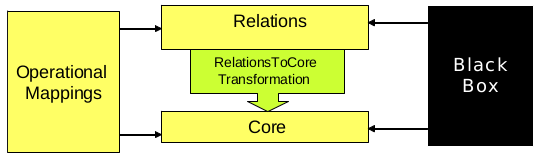
\includegraphics[scale=1.0]{figures/schemaQVTofficiel.png}
  \caption{Architecture du standard {\qvt}~\cite{omgqvt1}.}
  \label{fig:qvt}
\end{figure}
{\qvtr} et {\qvtc} constituent la partie déclarative de {\qvt}. {\qvtr} est un
langage orienté utilisateur avec une syntaxe textuelle et graphique permettant
de définir des transformations à un niveau d'abstraction élevé (représentation
graphique possible). {\qvtc} est quant à lui plus bas niveau avec uniquement
une syntaxe textuelle. Il sert à spécifier la sémantique de {\qvtr} sous la
forme d'une transformation \emph{Relations2Core}. L'expression d'une
transformation avec {\qvt} déclaratif est une association de motifs
(\emph{patterns}) entre la source et la cible. Bien que relativement complexe à
prendre en main, il permet de définir des transformations bidirectionnelles.
{\optimalj} était une implémentation commerciale de {\qvtc}, mais son
développement a cessé. Les outils
{\mediniqvt}\footnote{\url{http://projects.ikv.de/qvt/wikia}}, {\eclipsemmt}
(anciennement {\eclipsemtom}\footnote{\url{http://www.eclipse.org/m2m/}}) ainsi
que {\moment}~\cite{Boronat2009} implémentent quant à eux {\qvtr}.

Le langage {\qvto} supporte la partie impérative de {\qvt}. De par la nature
même du style impératif, la navigation et la création d'éléments du modèle
cible sont explicites. {\qvto} étend {\qvtr} et {\qvtc} par ajout de
constructions impératives telles que la séquence, la répétition, la sélection,
{\etc} ainsi que par des constructions {\ocl}. {\smartqvt} et
{\eclipsemmtoqvt} implémentent {\qvto}.

%\ttodo{à mettre ?}
%Le tableau\needcite{} résume la classification des outils implémentant {\qvt},
%selon qu'ils implémentent la partie déclarative ou impérative.
%\begin{tabular}[h]{m{2.5cm}m{5cm}}
% & \\
%  \hline
%Core & (OptimalJ (fini)\\
%Operational Mappings& Borland Together Architect 2006\newline SmartQVT\newline Eclipse M2M\newline ATL\\
%Relations & \mediniqvt\newline ModelDorf\newline MomentQVT\newline M2M, ATL\\
%\end{tabular}

%Comparaison QVTo vs QVTr, dans Guduric2009\\
%\begin{tabular}{m{0.25\linewidth}|m{0.35\linewidth}|m{0.35\linewidth}}
%Critère & QVT-Operational & QVT-Relational\\
%\hline
%Paradigme de programmation & impératif & déclaratif \\
%Niveau d'abstraction & bas niveau & haut niveau \\
%Traçabilité & unidirectionnelle & bidirectionnelle \\
%Compétences requises & répandues & rares, inhabituelles\\
%Scénarios de transfo & génération ou synchro dans 1 sens  & génération+synchro
%2 sens,
%contrôle de conformité, \\
%Niveau de contrôle & Précis & générique \\
%Complexité du code & Standard & Initialement complexe \\
%Organisation du code & Comme QVT-R + bibliothèques de transfo & héritage de
%transformation, surcharge de règles\\
%Représentation graphique & Inappropriée & Possible \\
%Outils & SmartQVT & mediniQVT \\
%\end{tabular}


\paragraph{\emph{{\qvt}-like}.}
%n'implémente pas à proprement parler le standard {\qvt}, cependant on peut le
%classer dans la catégorie des \emph{{\qvt}-like}, c'est-à-dire qu'il s'agit
%d'un langage de transformation similaire à {\qvt}. 
Les outils dont nous allons parler ici n'implémentent pas, à proprement parler,
le standard {\qvt}, mais sont cependant suffisamment proches et similaires pour
être souvent classés dans la catégorie des \emph{{\qvt}-like}. Le premier
d'entre eux est très certainement
{\atl}\footnote{\url{http://www.eclipse.org/atl/}}~\cite{Bezivin2003-firstExperiment,Bezivin2005,Jouault2006,JouaultABK08}
: il s'agit d'un des langages les plus utilisés dans la communauté des
modèles et est intégré dans l'environnement {\eclipse}~\cite{atl04}. Il permet
de spécifier une transformation d'un ensemble de modèles sources en un ensemble
de modèles cibles. Écrire un programme {\atl} consiste à écrire des règles
(\emph{rules}) en donnant une source et une cible. Une règle peut faire appel à
des fonctions d'aide (\emph{helper}) permettant d'effectuer un traitement
(collecte de valeurs dans une liste, \etc).
%\todo{\begin{itemize} \item ATL :~\cite{Bezivin2003-ATLTechReport}, premières
%XP~\cite{Bezivin2003-firstExperiment}({\xslt} into XQuery), plus
%récent~\cite{JouaultABK08}, \item Environnement Eclipse pour ATL~\cite{atl04}
%\item Traçabilité (\emph{loosely coupled}) :~\cite{Jouault2005} \item Modeling
%in Large, modeling in small :~\cite{Bezivin2005} \item Syntaxe ATL
%:~\cite{Jouault2006} \item Poster, fiche de résumé :~\cite{Jouault2006a} \item
%comparaison CGT vs AGG vs ATL :~\cite{Groenmo2009} \end{itemize}} Dans la
%suite du document, les exemples sur lesquels nous nous appuyons sont tous des
%exemples qui ont déjà été écrits en {\atl}. 
Outre {\atl}, d'autres outils \emph{{\qvt}-like} existent, notamment
{\tefkat}\footnote{\url{http://tefkat.sourceforge.net/}}~\cite{Lawley2006} (qui
propose une syntaxe à la {\sql} et offre une implémentation de {\qvtr}),
{\great}~\cite{Agrawal2003,Balasubramanian2007} et {\viatra}~\cite{Varro2007},
qui sont des outils de transformation de graphes. Ces deux derniers sont
distribués sous forme d'un \emph{plugin} {\eclipse} ce qui leur permet
d'interagir avec l'environnement {\emf}.  Enfin, dans cette catégorie d'outils,
nous pouvons ajouter
{\jqvt}\footnote{\url{http://sourceforge.net/projects/jqvt/}} qui est un moteur
{\qvt} pour {\java}. Il est intégré dans {\eclipse}, est compatible avec {\emf}
et n'utilise pas {\ocl}, mais
{\xbase}\footnote{\url{https://wiki.eclipse.org/Xbase}}.


\paragraph{\kermeta.} Il s'agit d'un environnement de métamodélisation dans
{\eclipse}. Il permet de définir et spécifier des langages de modélisation
dédiés. Le langage
{\kermeta}\footnote{\url{http://www.kermeta.org}}~\cite{kermeta10} mêle
plusieurs paradigmes de programmation (orienté objet, orienté
aspects~\cite{Muller2005,Muller2005a}, par contrats, fonctionnel) et fournit un
support complet de {\ecore} et de {\emof}. Ainsi, tout modèle {\kermeta}
conforme à {\emof} est aussi un programme {\kermeta} valide. Une définition
{\kermeta} peut être compilée pour produire un modèle exécutable. Le code
généré est exprimé en {\java} et {\scala}, qui peut être ensuite compilé pour
être exécuté sur la machine virtuelle {\java}.

%Le langage {\kermeta} repose sur 
%\ttodo{is'étendre un peu plus sur {\kermeta} ; parler de K2/K3 ; de la génération
%de code jvm/scala.}

%impératif

%kevoree\footnote{\url{http://kevoree.org}}
     



%\section{Validation et vérification du logiciel}
%intro, définitions, contraintes, outils
%
%\ttodo{augmenter la qualité du soft, la confiance dans le logiciel :
%vérification. Comment ? tests et simulation ; preuve mathématique ; MC
%(exploration d'espaces d'états, tests exhaustifs, recherche de contre-exemple)}
%
%Dans cette section, nous abordons différentes manières de valider et vérifier
%le logiciel afin d'en améliorer sa qualité, et donc la confiance que
%l'utilisateur peut avoir dans les logiciels qu'il utilise.
%
%\ttodo{pourquoi ai-je écrit ces 4 paragraphes ? utile ou pas ?}
%
%\paragraph{Tests.}Une première approche, intuitive, est de tester intensément
%tout programme informatique avant sa mise en production. Il existe diverses
%méthodologies et techniques pour tester du code. On citera par exemple la mise
%en place de tests unitaires censés tester des \emph{unités} de code (fonctions,
%classes). Cela a été popularisé par les méthodes agiles, et particulièrement
%par l'approche dirigée par les tests (\emph{Tests Driven Engineering}). Bien
%que l'utilisation de tests permette d'améliorer grandement la qualité du
%logiciel durant sa phase de développement, la solution des tests unitaires
%commence à montrer ses limites lors de développements de logiciels complexes où
%les \emph{bugs} peuvent avoir des origines plus nombreuses. Du fait des coûts
%et des délais de développement, il n'est pas rare de ne pas écrire de tests
%pour se concentrer sur le logiciel lui-même. Par conséquent, certains morceaux
%de code ne sont pas testés et sont donc susceptibles de recéler des
%\emph{bugs}. Des techniques de génération automatique de tests ont vu le jour
%\ttodo{quelques réf aussi} pour augmenter la couverture de tests et tester au
%maximum les cas limite. D'autres comportements anormaux peuvent aussi naître
%d'une combinaison de comportements normaux de modules fonctionnels
%indépendamment. Le problème pouvant alors provenir d'une incompréhension entre
%les équipes de développeurs, ou entre le client et le fournisseur
%(spécification ambiguë).\\ 
%Cependant, si l'intégration de tests est absolument nécessaire dans le
%processus de développement d'un logiciel, elle se révèle insuffisante dans le
%cas du logiciel critique. En effet, tester intensément un logiciel permet
%de tester son comportement dans la plupart des cas, mais rien ne garantit que
%toutes les situations ont été testées.\ttodo{un peu de contexte sur le test} 
%
%\paragraph{Preuve.}À l'opposé, une autre approche pour améliorer la confiance
%dans un logiciel consiste à prouver mathématiquement les algorithmes. Le
%problème étant alors que la preuve formelle est généralement faite sur les
%algorithmes ou les spécifications, mais pas sur l'implémentation elle-même. Or,
%le facteur humain n'est pas à négliger, l'implémentation concrète du logiciel
%dépendant fortement du développeur et des outils utilisés durant le processus.
%En outre, lors d'une preuve, le contexte réel n'est pas forcément pris en
%compte et certaines conditions d'utilisation réelles peuvent fortement
%influencer le comportement et la fiabilité de l'application.
%\ttodo{petite réf sur les protocoles réseau ? protocole ethernet ? gap pratique
%vs théorie car phénomènes physiques (bruit), ou alors physique, bio}\\
%\todo{"Beware of bugs in the above code; I have only proved it correct, not
%tried it." --- D.E.Knuth}
%
%
%\paragraph{Simulation.}Pour répondre à ce problème de réalisme du comportement
%d'une système sous conditions d'utilisation réelles, une approche liée aux
%tests revient à simuler ou émuler le système pour étudier son comportement et
%détecter les anomalies. L'intérêt de ce type d'approche est que l'on peut
%travailler sur un système qui serait coûteux à déployer en conditions réelles.
%Notons par exemple les domaines du nucléaire ou de l'avionique \ttodo{référence
%à l'A380 entièrement simulé ?} qui ne permettent pas aisément des tests
%logiciels en conditions réelles, en particulier lors des premières étapes de
%développement. \ttodo{réf aux gens qui font de la simulation pour \emph{tester} ?}
%
%Par rapport une preuve formelle, les méthodes de tests ont aussi l'inconvénient
%d'être fortement conditionnées par la plateforme sur lesquels els sont exécutés
%et par les technologies employées.
%
%\paragraph{Model-checking.}Le \emph{model-checking} est une autre approche
%entre preuve et test. Elle consiste modéliser un système selon un formalisme
%donné, puis à explorer les espaces d'états possibles de ce système pour le
%valider. Cela revient à du test exhaustif, ce qui a donc valeur de preuve.
%L'intérêt du \emph{model-checking} est que ---~contrairement aux tests~--- il est
%généralement indépendant de la plateforme d'exécution et qu'il apporte une
%validation formelle du système. On peut toutefois reprocher au
%\emph{model-checking} de ne pas toujours être proche de la réalité et d'avoir
%un coût en ressources élevé dans le cas de systèmes complexes. Cela a conduit
%certains à adopter des approches hybrides de \emph{model-checking} à
%l'exécution sur des applications réelles simulées \ttodo{réf. à ceux qui font
%du MC sur des binaires à run-time par ex ? domaine différent, mais un peu lié}.
%
%Dans le cadre du développement de logiciels critiques, la vérification des
%applications est imposée par la loi et des normes à respecter. Ainsi, tout
%logiciel critique devant être embarqué dans un avion doit suivre une procédure
%de certification.
%
%\todo{problèmes : \begin{itemize}
%    \item outils de modélisation non qualifiés et non certifiés => certifier
%      des outils ou aider à certifier
%    \item pb {\mde} : beaucoup d'outils dans les chaînes de développement => introduction des
%outils "certifieurs" automatiques, problématique
%\end{itemize}}
%
%\subsection{Qualification}
%\ttodo{définir, expliquer, donner les normes, dont DO-XXX}
%
%La qualification d'un logiciel participe à atteindre un objectif.
%
%
%
%\subsection{Certification}
%\ttodo{définir, expliquer.}
%
%
%\ttodo{Différences entre qualification et certification.}
%Problématiques : traçabilité, séparer spécification/implémentation/vérification
%
%
%\section{Traçabilité}
%ici ? traçabilité interne vs traçabilité de spécification ; intérêt (contrainte
%des précédentes sous-sous-sections). Souvent traçabilité interne ou fortement
%liée à l'implémentation de la transformation. Se fait bien techniquement.
%
\section{Limitations actuelles et points d'amélioration}

Le lancement de l'initiative {\mda} a donné un véritable élan à l'{\idm} et de
nombreux outils ont vu le jour. Cependant, malgré l'intérêt indéniable de
cette approche pour le développement logiciel, l'{\idm} n'est pas encore
fortement établie dans les chaînes de développement industrielles et gagne
lentement du terrain.

La complexité des systèmes s'accroissant, l'industrie voit dans l'{\idm} une
solution pour améliorer leur développement tout en diminuant leurs coûts. En
effet, pour appréhender cette complexité, il est nécessaire pour les
développeurs d'abstraire les problèmes. Pour ce faire, il faut des outils
accessibles et utilisables dans un cadre industriel. 

La grande diversité des outils peut aussi être un frein à l'adoption des
techniques de l'{\idm} : un trop grand nombre d'outils et de technologies
segmente le domaine, ce qui peut empêcher que les communautés atteignent une
masse critique. De plus, beaucoup d'outils adoptant les concepts de l'{\idm}
sont issus de la recherche et sont utilisés par un public académique.  N'ayant
pas forcément vocation à industrialiser les prototypes développés, le monde de
la recherche produit souvent des outils peu accessibles tant sur leur forme
(ergonomie, non conformité aux pratiques industrielles habituelles) que sur le
fond (concepts peu connus et maîtrisés par peu de monde, expertise nécessaire).
Ce frein lié à la multiplicité des outils peu accessibles peut être levé par
l'établissement de standards tels que ceux proposés par l'{\omg}, ainsi que par
le déploiement d'environnements comme {\eclipse} pour pousser à la
cristallisation et au développement de communautés autour des technologies
liées. 

Un autre aspect limitant vient de l'adaptation des chaînes de développement
logicielles existantes à ces nouvelles méthodes de développement et à ces
nouveaux outils. Compte tenu de leur coût d'intégration et des
changements induits par une telle modification d'un processus de développement,
il n'est pas raisonnable d'adopter un nouvel outil encore à l'état de prototype
ou nécessitant des compétences spécifiques maîtrisées par un petit nombre 
d'experts ou encore n'ayant aucun lien avec des technologies déjà présentes
dans la chaîne de développement existante. Il faut donc mettre en œuvre des
ponts entre les technologies pour les rendre plus attrayantes et plus
facilement intégrables, afin de faciliter ce processus fortement consommateur
de ressources.

Outre l'adaptation normale des chaînes de développement aux nouveaux outils,
certains domaines ont des contraintes strictes de qualité concernant les outils
de production du logiciel. C'est le cas des chaînes de développement des
systèmes critiques que l'on retrouve notamment en aéronautique, dans le secteur
automobile, ainsi que dans celui de la santé. Les logiciels produits et servant
à produire sont soumis à des exigences légales nécessitant des processus lourds
de validation du logiciel. Le domaine de l'{\idm} étant relativement
jeune, il n'est pas encore pleinement adopté dans ce type d'industrie qui a
besoin d'outils adaptés à ses contraintes permettant de faciliter la validation
du logiciel à moindre coût (et présenter ainsi un intérêt supérieur par rapport
à l'existant).

L'un des aspects les plus intéressants est l'usage de l'{\idm} dans le cadre du
développement fiable : pour les problématiques légales évoquées précédemment, la
demande industrielle est très forte, et peu de réponses concrètes existent ou
alors pour des coûts déraisonnables. C'est dans ce contexte que nous nous
proposons d'apporter un élément de solution avec ce travail, afin d'accompagner
l'adoption de nouveaux outils tout en améliorant la qualité du logiciel. Nous
abordons la problématique de la validation du logiciel dans le
chapitre~\ref{ch:verification}.

%\todo{limitations dans quel contexte ? 
%\begin{itemize}
%\item {\idm} : multiplication des outils
%\item souci validation avec beaucoup d'outils (contexte)
%\item approches actuelles coûteuses
%\item on pourrait apporter des outils pour faciliter la validation, et
%augmenter la confiance dans le logiciel
%\item technique : choix des outils ; DSL vs GPL ; framework
%\item traçabilité : trace exploitable -> on va en parler plus tard, dans le
%  chapitre suivant
%\end{itemize}}




% vim:spell spelllang=fr


%\DontFrameThisInToc
% vim:spell spelllang=fr
\chapter{Vérification du logiciel}
\label{ch:verification}
%10p

%exemple heartbleed : 
%http://xkcd.com/1354/
%http://imgs.xkcd.com/comics/heartbleed_explanation.png

Il est extrêmement difficile de garantir l'absence totale d'erreurs
dans un logiciel. Et cette tâche est d'autant plus ardue que le logiciel est
complexe. Les bogues pouvant avoir des conséquences désastreuses et
coûteuses, il est nécessaire de valider, vérifier et tester le logiciel avant
leur mise en production. Dans ce chapitre, nous présentons le contexte de la
vérification du logiciel dans lequel ce travail s'inscrit.  Nous expliquons
différentes approches pour vérifier le
logiciel~\ref{ch:verification:sec:approches}. Nous présentons aussi la
qualification et la certification~\ref{ch:verification:sec:certifqualif} qui
exigent une traçabilité.


%Therac-25 (juillet 1985 -> avril 1986) / Ariane 5 (4 juin 1996) / crash AT&T (15 janvier 1990) / Pentium (juin 1994) / banque de New-York (21 novembre 1985)

%\todo{VVT : Validation, Vérification, Test}

%ch3 : validation et vérification des transformations -> biblio
%
%approches pour le logiciels -> relecture, testes
%approches formelles, s'appuient sur spécification -> preuves, MC
%certification, qualification
%=> exigences ; préserver la traçabilité exigences/spécification
%Notre cadre : qu'est-ce qui existe, biblio dessus
%
%approche «  validation par la traduction »

\section{Approches pour la vérification du logiciel}
\label{ch:verification:sec:approches}
%intro, définitions, contraintes, outils

%\ttodo{augmenter la qualité du soft, la confiance dans le logiciel :
%vérification. Comment ? tests et simulation ; preuve mathématique ; MC
%(exploration d'espaces d'états, tests exhaustifs, recherche de contre-exemple)}

Dans cette section, nous abordons différentes manières de vérifier le logiciel
afin d'en améliorer sa qualité, et donc la confiance que l'utilisateur peut
avoir dans les logiciels qu'il utilise. Nous présentons d'abord des approches
logicielles pratiques comme la relecture, les tests et la simulation, puis la
preuve et le \emph{model-checking} qui sont des approches formelles.
%~\ref{ch:verification:subsec:relecture},
%les tests~\ref{ch:verification:subsec:test} et la
%simulation~\ref{ch:verification:subsec:simu}, puis la
%preuve~\ref{ch:verification:subsec:preuve} et le
%\emph{model-checking}~\ref{ch:verification:subsec:mc} qui sont des approches
%formelles.% Nous évoquons aussi une approche qui peut être vue comme un
%%compromis : la simulation~\ref{ch:verification:subsec:simu}.
Ces méthodes pour vérifier le logiciel et améliorer sa qualité sont
généralement utilisées de manière conjointe, selon le niveau d'exigence visé
(les contraintes pour une application sur ordiphone ne sont pas les mêmes que
pour celles d'un calculateur de vol).

\subsection{Relecture}
\label{ch:verification:subsec:relecture}

Une première approche évidente pour tout développeur est la relecture de code.
Informelle, elle consiste à parcourir du code développé précédemment et à
s'assurer qu'il est conforme aux exigences. Pour améliorer la fiabilité d'une
relecture, la tendance est de faire relire du code d'un développeur à un autre
développeur n'ayant pas participé au développement, et de croiser les
relectures. Cependant, si cette méthode est largement répandue et encouragée,
elle est loin d'être fiable. En effet, la relecture dépend totalement d'un
relecteur humain dont l'état au moment de la relecture (compétences, fatigue,
concentration, etc.) conditionne le résultat. Si la relecture permet de repérer
les bogues les plus évidents, elle permet difficilement de repérer les plus
subtils. De plus, dépendant des compétences et de l'expérience du relecteur,
cette méthode est fortement soumise à son intuition. Une vérification d'un
logiciel par relecture pourra ainsi être très différente selon le développeur.
Si la relecture est indispensable dans tout développement, elle n'est pas
suffisante pour du logiciel exigeant une forte fiabilité. Elle présente
toutefois l'avantage d'être naturelle à tout développeur ayant suivi une
formation adéquate\footnote{La relecture fait partie intégrante de la
méthodologie du développement généralement enseignée dans les formations en
informatique.} et d'être peu coûteuse : en effet, elle ne nécessite pas de
compétences et d'outils supplémentaires qu'il a été nécessaire pour écrire le
logiciel à relire. Cette approche de vérification peut éventuellement être
suffisante pour des applications peu complexes, non critiques et peu diffusées
(par exemple : un script pour renommer des fichiers dans un répertoire
personnel). Elle reste efficace pour trouver des erreurs et constitue un
élément fondamental de certaines approches agiles.


\subsection{Tests}
\label{ch:verification:subsec:test}

Une seconde approche est de tester tout programme informatique avant sa mise en
production, l'intensité des tests permettant d'obtenir plus d'assurance. Il
existe diverses méthodologies et techniques pour tester du code. On citera par
exemple la mise en place de tests unitaires censés tester des \emph{unités} de
code (fonctions, classes). Des \emph{frameworks} dédiés aux tests unitaires ont
ainsi été développés, comme par exemple
{\junit}\footnote{\url{http://www.junit.org}}. Cela a été popularisé par les
méthodes agiles, notamment \emph{eXtreme Programming}~\cite{Beck2004} qui
repose en partie sur l'approche dirigée par les tests (\emph{Tests Driven
Development}~\cite{Beck2003}). Remarquons que les scénarios de tests peuvent
être considérés comme une forme de spécification. Bien que l'utilisation de
tests permette d'améliorer grandement la qualité du logiciel durant sa phase de
développement en réduisant les défauts~\cite{Williams2003}, la solution des
tests unitaires commence à montrer ses limites lors de développements de
logiciels complexes où les bogues peuvent avoir des origines plus nombreuses.
Du fait des coûts et des délais de développement, il n'est pas rare de ne pas
écrire de tests pour se concentrer sur le logiciel lui-même. Par conséquent,
certaines parties de code ne sont pas testées et sont donc susceptibles de
contenir des bogues. Des techniques de génération automatique de tests ont vu
le jour pour augmenter la couverture de tests et tester au maximum les cas
limites. Nous noterons par exemple 
%l'outil DART~\cite{Godefroid2005}
{\quickcheck}~\cite{Claessen2000,Hughes2010} pour tester les programmes
{\haskell}, ainsi que ses implémentations et variantes pour d'autres langages
%telles que {\scalacheck}\footnote{\url{http://code.google.com/p/scalacheck/}}
%pour {\scala}, {\propcheck}\footnote{\url{https://github.com/polux/propcheck}}
%pour le langage {\dart}, {\quickcheck} pour
%{\java}\footnote{\url{https://bitbucket.org/blob79/quickcheck}}~\cite{Earle2013},
%{\rushcheck}\footnote{http://rushcheck.rubyforge.org/} pour {\ruby}, {\etc}
%\ttodo{autres réf et outils ?
%{\junitquickcheck}\footnote{\url{https://github.com/pholser/junit-quickcheck}},
%{\jcheck}\footnote{\url{http://www.jcheck.org/}}, qc = quickcheck pour Python
%\footnote{http://github.com/dbravender/qc}}.
% 
  tels que {\scala}\footnote{{\scalacheck} :
  \url{http://code.google.com/p/scalacheck/}}, {\dart}\footnote{{\propcheck} :
  \url{https://github.com/polux/propcheck}}, {\java}\footnote{{\quickcheck}
  pour {\java}~\cite{Earle2013} :
  \url{https://bitbucket.org/blob79/quickcheck}}, {\ruby}\footnote{{\rushcheck}
  : \url{http://rushcheck.rubyforge.org/}}, {\python}\footnote{qc :
    \url{http://github.com/dbravender/qc}}, {\etc}



Ces méthodes ont été transposées dans le cadre de l'{\idm}. L'approche dirigée
par les tests~\cite{Giner2009} s'est développée, et des travaux de vérification
par le test ont été menés pour les transformations de
modèles~\cite{Fleurey2004}. Des \emph{frameworks} de test~\cite{Lin2005}, ainsi
que des outils de génération de tests~\cite{Brottier2006,Lamari2007,Sen2009} et
de génération de code tests~\cite{Rutherford2003} ont donc aussi vu le jour,
accompagnés d'outils et de techniques de qualification des données de tests
pour les transformations de modèles~\cite{Fleurey2009}.

Les tests permettent de détecter des comportements anormaux, mais d'autres
comportements anormaux peuvent aussi naître d'une combinaison de comportements
normaux de modules fonctionnels indépendamment. Le problème pouvant alors
provenir d'une incompréhension entre les équipes de développeurs ou entre le
client et le fournisseur (spécification ambiguë). Si l'intégration de tests est
absolument nécessaire dans le processus de développement d'un logiciel, elle se
révèle insuffisante dans le cas du logiciel critique. En effet, tester
intensément un logiciel permet de tester son comportement dans la plupart des
cas, mais rien ne garantit que toutes les situations ont été testées.

%\ttodo{théorie des graphes pour valider les transformations de modèles~\cite{Kuester2006}} 

\subsection{Simulation}
\label{ch:verification:subsec:simu}

Il peut aussi être extrêmement difficile de tester correctement un système du
fait de sa complexité, des fortes ressources demandées ou de la particularité
de sa plateforme d'exécution. Les tests écrits et menés durant le développement
peuvent se révéler peu réalistes ou fort éloignés des conditions réelles
d'utilisation. Pour répondre à ce problème de réalisme du comportement d'un
système sous conditions d'utilisation réelles, une approche liée aux tests
revient à simuler le système pour étudier son comportement et
détecter les anomalies. L'intérêt de ce type d'approche est que l'on peut
travailler sur un système qui serait coûteux à déployer pour tester en
conditions réelles. Notons par exemple les domaines du nucléaire ou de
l'avionique qui ne permettent pas aisément (et à faible coût) des tests
logiciels en conditions réelles, en particulier lors des premières étapes de
développement. L'inconvénient de ce type de méthode de vérification est qu'il
faut reproduire fidèlement un environnement et que les tests sont fortement
conditionnés par la plateforme d'exécution sur lesquels ils sont exécutés et
par les technologies employées. Dans le cas d'une informatique simple, la
simulation est une option intéressante, mais sa difficulté de mise en œuvre
croît avec la complexité du système (nombreuses dépendances, systèmes
exotiques, matériel non disponible hors chaîne de production dédiée, modèles
physiques complexes, {\etc}). Ainsi, en aéronautique, il est extrêmement
complexe et coûteux de modéliser intégralement l'environnement afin de simuler
tous les systèmes de l'avion. L'approche adoptée revient alors à procéder à une
succession de phases simulant des modèles de l'environnement mécanique,
physique, des calculateurs, du réseau, du logiciel, {\etc} La dernière étape
avant le vol réel est l'\emph{Aircraft Zero --- Iron Bird} qui intègre toute
l'informatique réelle sur un banc d'essai.

%Par rapport à une preuve formelle, les méthodes de tests ont aussi
%l'inconvénient d'être fortement conditionnées par la plateforme sur lesquels
%ils sont exécutés et par les technologies employées.


\subsection{Preuve}
\label{ch:verification:subsec:preuve}

À l'opposé de ces approches vues comme très pragmatiques et largement utilisées
dans l'industrie, une autre approche pour améliorer la confiance dans un
logiciel consiste à prouver formellement les algorithmes. Le problème est alors
formalisé sous la forme d'axiomes et de buts qu'il faut atteindre en démontrant
des théorèmes. Une preuve mathématique peut être écrite à la main, mais pour
faciliter le processus et pour diminuer les risques d'introduction d'erreurs
liées au facteur humain, des outils assistants à la preuve tels que
{\coq}~\cite{Coq,Bertot2004} et {\isabelle}~\cite{Nipkow2002} ont été
développés. Une preuve {\coq} est censée donner une forte confiance dans le
logiciel développé et prouvé. Cependant, si la preuve de la correction d'un
algorithme donne une garantie irréfutable du bon comportement de cet
algorithme, elle ne donne pas obligatoirement la garantie du bon comportement
du logiciel. En effet, ce sont les algorithmes et les spécifications qui sont
généralement formellement prouvés et non les implémentations
elles-mêmes\footnote{\og Beware of bugs in the above code; I have only proved
  it correct, not tried it \fg{} -- D.E.  Knuth, 1977 ; citation et explication
  accessibles sur sa page personnelle :
  \url{http://www-cs-faculty.stanford.edu/~uno/faq.html}}. Or, le facteur
  humain n'est pas à négliger, l'implémentation concrète du logiciel dépendant
  fortement du développeur et des outils utilisés durant le processus. En
  outre, lors d'une preuve, le contexte réel n'est pas forcément pris en compte
  et certaines conditions d'utilisation réelles peuvent fortement influencer le
  comportement et la fiabilité de l'application. %On peut aussi effectuer un
%  raffinement pour finalement extraire le programme depuis la preuve {\coq}.

%\ttodo{réf sur du réel qui ne colle pas avec la preuve : réseau ? gap pratique
%vs théorie car phénomènes physiques (bruit), ou alors physique, bio\\ Preuve de
%transformation de modèles ?}


\subsection{Model-checking}
\label{ch:verification:subsec:mc}

%?\cite{Jhala2009} survey sur le MC

Le \emph{model-checking} est une autre approche formelle que l'on peut
considérer comme étant entre preuve et test. Elle consiste à abstraire
(modéliser) un problème ou un système selon un formalisme (langage) donné, puis
à explorer l'espace d'états possibles de ce système pour vérifier qu'aucun
état ne viole une propriété donnée (un invariant par exemple). On peut
considérer que cela revient à du test exhaustif, ce qui a donc valeur de
preuve. L'intérêt du \emph{model-checking} est que --- contrairement aux tests
--- il est généralement indépendant de la plateforme d'exécution et qu'il
apporte une vérification formelle du système. Par exemple, les outils
{\cadp}\footnote{\url{http://cadp.inria.fr}}~\cite{Garavel2011} et
{\tina}\footnote{\url{http://projects.laas.fr/tina}}~\cite{Berthomieu2004} sont
deux \emph{model-checkers} dont les formalismes d'expression des modèles sont
respectivement LOTOS et les réseaux de Petri. On peut toutefois reprocher au \emph{model-checking} de ne pas
toujours être suffisamment proche de la réalité et d'avoir un coût en
ressources élevé dans le cas de systèmes complexes. Cela a conduit certains à
compléter le \emph{model-checking} par l'analyse à l'exécution sur des
applications réelles simulées~\cite{Bayazit2005}. L'{\idm} reposant sur les
modèles qui sont des abstractions de problèmes, il est naturel d'adopter le
\emph{model-checking} pour vérifier le logiciel produit par ces méthodes. On
peut adjoindre des contraintes aux modèles avec des langages tels qu'{\ocl}
dans le cas de {\uml}, mais un modèle n'est pas nécessairement immédiatement
vérifiable. Il nécessite souvent une ou plusieurs transformations afin de
pouvoir être vérifié au moyen d'un \emph{model-checker}. C'est une approche
courante que d'opérer une suite de transformations permettant de passer du
modèle servant de spécification au modèle vérifiable, ainsi que de la
spécification vers l'application réelle.  Cependant, comme précédemment, il
s'agit à nouveau de vérifier un modèle et non pas le code généré réel. Chaque
transformation se doit donc d'être simple afin que l'on puisse garantir la
préservation du comportement d'un pas à l'autre. Ce type d'approche est très
utilisé en {\idm}. Nous notons immédiatement qu'une telle approche pour
s'assurer du bon fonctionnement du logiciel nécessite non seulement une
vérification du modèle, mais aussi une garantie que la transformation elle-même
est correcte.

\section{Certification et qualification}
\label{ch:verification:sec:certifqualif}
%\todo{transfos de modèles, deux formes de vérification : 
%\begin{itemize}
%  \item avant la transfo une fois pour toutes
%  \item après chaque utilisation de la transformation
%\end{itemize}
%Le niveau de certification demandé ainsi que l'utilisation des outils impliqués
%dans le processus de développement de logiciel embarqué impose de vérifier les
%outils.
%}

Le processus de certification n'est pas nécessaire pour tous les logiciels et
tous les secteurs d'activité. Il fait en revanche partie intégrante du
processus de développement logiciel dans le cadre de développement de systèmes
critiques, par exemple dans les domaines de l'aéronautique, de l'automobile (du
transport en général) et de la santé. La loi impose le respect d'exigences en
fonction de crédits de certification demandés. 

\begin{definition}[Crédit de certification]
  Acceptation par l'autorité de certification qu'un processus, un produit ou
  une démonstration satisfait les exigences de certification.
\end{definition}

\begin{definition}[Certification]
  Processus d'approbation par une autorité de certification d'un produit.
\end{definition}

%\begin{definition}[Autorité de certification]
%  Entité en charge de l'approbation des données de qualification d'outil.
%\end{definition}

Ces exigences sont fixées par des standards de certification : en aéronautique,
le standard actuel est la norme DO-178C/ED-12C\footnote{La notation DO-
correspond au nom donné à ce standard aux États-Unis d'Amérique, tandis que la
notation ED- est celle en vigueur en Europe.}~\cite{DO-178C}. Elle donne des
objectifs (et non des moyens) dont le nombre et le niveau augmentent avec le
niveau de criticité. Ces niveaux de criticité (ou niveaux DAL, pour
\emph{Development Assurance Level}) sont notés de A à E, A étant le plus
critique, E le moins critique : 

\begin{enumerate}[\text{Niveau} A :]

  \item (Erreur catastrophique) un défaut du système ou sous-système étudié
    peut provoquer un problème catastrophique (sécurité du vol ou atterrissage
    compromis, crash de l'avion) ;

  \item (Erreur dangereuse) un défaut du système ou sous-système étudié peut
    provoquer un problème majeur entraînant des dégâts sérieux voire la mort de
    quelques occupants ;

  \item (Erreur majeure) un défaut du système ou sous-système étudié peut
    provoquer un problème sérieux entraînant un dysfonctionnement des
    équipements vitaux de l'appareil (pas de mort) ;

  \item (Erreur mineure) un défaut du système ou sous-système étudié peut
    provoquer un problème pouvant perturber la sûreté du vol (pas de mort) ;

  \item (Erreur sans effet) un défaut du système ou sous-système étudié peut
    provoquer un problème sans effet sur la sûreté du vol.

\end{enumerate}

Dans le cadre du processus de certification de systèmes critiques, les outils
utilisés pour le développement doivent être vérifiés afin de s'assurer de leur
bon fonctionnement et qu'ils n'introduisent pas d'erreurs dans le logiciel.

Les pratiques de développement logiciel évoluant, notamment par l'adoption
croissante de l'approche dirigée par les modèles qui plaide pour
l'automatisation maximale des tâches, de nouveaux outils sont intégrés aux
processus de développement. L'introduction d'outils automatiques dans une
chaîne de développement de système soumis à certification impose l'une des deux
approches suivantes :
\begin{itemize}
  \item vérifier les données produites par l'outil \emph{a posteriori} ;
  \item qualifier l'outil.
\end{itemize}

%\todo{Crédit de certification = confiance dans l'outil\\
%Crédit de certification implicite : pas de vérification des sorties de l'outil. 
%Si vérification des sorties, qualification pas requise}

La qualification d'un logiciel participe à atteindre un objectif exigé par le
processus de certification et permet d'obtenir de la confiance dans les
fonctionnalités d'un outil. Ce processus de qualification peut être appliqué à
une ou plusieurs fonctions dans un outil, à un outil unique ou à un ensemble
d'outils.

\begin{definition}[Qualification]
La qualification d'outils est le processus nécessaire pour obtenir des crédits
de certification d'un outil. Ces crédits peuvent uniquement être garantis pour
un usage donné dans un contexte donné.
\end{definition}

L'intérêt de la qualification d'un outil est d'obtenir suffisamment de
confiance en cet outil pour pouvoir l'intégrer dans une chaîne de développement
sans avoir à vérifier ses données de sortie ensuite. Le choix entre l'approche
de qualification et de vérification \emph{a posteriori} revêt un aspect
stratégique : si la qualification d'un outil peut avoir un coût élevé fixe,
elle n'en génère pas plus par la suite, tandis que la vérification \emph{a
posteriori} aura un coût récurrent.

%\todo{Qualification pas directement utilisée : focus sur les générateurs de code
%  critères :
%\begin{enumerate}
%  \item outils dont la sortie appartient au logiciel embarqué / compilo
%  \item outils qui automatisent un processus : détection d'erreur, (outils de
%    vérif formelle) / vérification
%  \item outils de vérification / pas d'impact
%\end{enumerate}}

La DO-178/ED-12 définit des catégories d'outils (\emph{sans impact},
\emph{vérification} et \emph{compilateur, générateur de code}) ainsi que des
critères de qualification. Elle précise les exigences de qualification adaptées
aux différents types d'outils et à leur utilisation. La norme
DO-330/ED-251~\cite{DO-330} donne des instructions pour la qualification
d'outils. Elle définit aussi cinq niveaux de qualification d'outils (TQL ---
\emph{Tool Qualification Levels}) qui sont fonction de ces trois critères ainsi
que de la criticité du logiciel développé :
\begin{enumerate}

  \item[TQL-1 à 3 : ] ces niveaux concernent les générateurs de code et outils
    dont la sortie fait partie du logiciel embarqué et qui peuvent donc
    introduire des erreurs ;
  
  \item[TQL-4 à 5 : ] ces niveaux concernent les outils de vérification, qui ne
    peuvent pas introduire d'erreurs, mais qui peuvent échouer à en détecter
    (outils de tests, analyseurs de code statique)

\end{enumerate}

Selon son utilisation et selon le type de production de l'outil, le niveau de
qualification sera différent. Un outil ne peut donc être qualifié une fois pour
toutes. En revanche, il peut être \emph{qualifiable} pour chaque projet,
c'est-à-dire \emph{pre qualifié} pour chaque projet.

%%%%%

L'{\idm} plaidant pour l'automatisation des tâches et l'usage d'outils
automatisant les tâches, il faut vérifier ces outils. Dans ce contexte, l'un
des problèmes majeurs de l'{\idm} est le grand nombre d'outils  non qualifiés
et non certifiés impliqués dans les chaînes de développement, notamment des
générateurs de code, des outils de traduction, et de manière plus générale des
outils automatisant au maximum les tâches de transformation. 
%Il faut donc certifier ou aider à certifier les nouveaux logiciels produits par
%ces nouvelles chaînes, et donc qualifier les outils.


%De plus, le processus de qualification étant mené manuellement par un humain,
%il est extrêmement coûteux et est sujet à erreurs. C'est dans ce contexte que
%notre travail s'intègre et que nous nous proposons d'aider le processus de
%qualification.


%validation = respect des besoins\\
%vérification = respect des specs

%\begin{definition}[Validation logicielle]
%Selon le standard~\cite{IEEEstd610}, il s'agit du processus d'évaluation d'un
%logiciel pendant ou à la fin du processus de développement pour déterminer s'il
%satisfait les exigences spécifiées.
%\end{definition}
%selon~\cite{DO-330} : Le processus qui détermine que les exigences sont les exigences
%corrects et qu'elles sont complètes.

%\begin{definition}[Vérification logicielle]
%Selon le~\cite{IEEEstd610}, il s'agit du processus d'évaluation d'un logiciel
%pour déterminer si le produit d'une phase de développement donnée satisfait les
%conditions imposées au début de cette phase. 
%\end{definition}
%selon~\cite{DO-330} : L'évaluation des sorties d'un processus pour s'assurer de la
%correction et de la cohérence en fonction des entrée fournies à ce processus.


%La validation logicielle garantit que le produit remplit effectivement les
%besoins client, et que les spécifications étaient correctes initialement, alors
%que la vérification garantit que le produit a été construit en conformité avec
%les exigences et les spécifications de conception. La validation garantit « que
%l'on a construit le bon produit ». La vérification garantit « que l'on a bien
%construit le produit ». La validation confirme que le produit fourni remplira
%l'usage attendu.

%translation validation =  validation après chaque exécution du compilateur
%que sa traduction est correcte (code cible correspond à une traduction correcte
%du code source)
%\todo{problèmes : 
%  \begin{itemize}
%    \item outils de modélisation non qualifiés et non certifiés => certifier
%      des outils ou aider à certifier
%    \item pb {\mde} : beaucoup d'outils dans les chaînes de développement =>
%      introduction des outils "certifieurs" automatiques, problématique
%\end{itemize}}

%Problématiques : traçabilité, séparer spécification/implémentation/vérification

\section{Traçabilité}
\label{ch:verification:trace}

%\todo{ici ? traçabilité interne vs traçabilité de spécification ; intérêt
%(contrainte des précédentes sous-sous-sections). Souvent traçabilité interne ou
%fortement liée à l'implémentation de la transformation. Se fait bien
%techniquement.}

%La qualification exige de séparer spécification, implémentation et
%vérification. Elle exige aussi d'assurer la traçabilité entre elles.

Une problématique fondamentale des compilateurs dans le cadre de la
certification d'un logiciel est d'assurer la traçabilité entre le code source
et le code binaire, ce qu'exige la norme DO-178/ED-12. Cette exigence pour les
compilateurs et générateurs de code est généralisable à toutes les
transformations, donc aux transformations de modèles à partir desquelles les
logiciels sont produits. Assurer cette traçabilité permet aussi de respecter la
contrainte de séparation de le spécification, de l'implémentation et de la
vérification tout en étant capable de relier les unes aux autres.

% ? ex de B2llvm : générateur B vers le langage intermédiaire de LLVM
% spéc B -> code intermédiaire ; activation de la traçabilité génère des
% commentaires lisibles humainement. mais rien de réutilisable automatiquement
% pour vérifier des propriétés.

\begin{definition}[Traçabilité]
  La norme DO-330~\cite{DO-330} définit la traçabilité comme une association
  entre objets telle qu'entre des sorties de processus, entre une sortie et son
  processus d'origine, ou entre une spécification et son implémentation.
\end{definition}

L'{\idm} plaidant pour l'automatisation maximale des tâches répétitives et
l'utilisation de générateurs de code pour produire le logiciel à partir de
modèles, il est nécessaire de vérifier les transformations qui en sont le cœur.
L'un des angles d'attaque du problème de la qualification est de fournir des
outils de transformations qualifiables, qui assurent la traçabilité des
transformations. 

Dans le cas d'une transformation de modèle, le métamodèle source fait partie de
la spécification et le modèle source la donnée d'entrée. Il convient donc de
conserver une trace de la transformation en maintenant un lien entre la source
et la cible. On retrouve souvent deux situations :

\begin{itemize}

  \item la trace se fait au niveau macroscopique (modèle d'entrée et modèle de
    sortie) et la granularité est extrêmement faible, ce qui rend la trace peu
    informative ;

  \item la trace s'opère de manière très détaillée (comme un \emph{debug}) ce
    qui génère une trace importante de tout ce qui s'est produit durant la
    transformation. Si toutes les informations sont présentes, se pose le
    problème de la pertinence des données recueillies : la quantité
    d'informations peut rendre la trace inexploitable, les éléments
    jugés intéressants risquant d'être noyés dans la trace.

\end{itemize}

Outre le respect strict des exigences de qualification, les informations de
trace peuvent être très utiles pour des tâches telles que le \emph{debugging}
ou l'analyse d'impact (conséquences d'une modification).

La traçabilité des transformations de modèle est un aspect important que la
plupart des outils traitent en apportant un support dédié, comme pour les
outils {\qvt}, {\atl}, {\tefkat} ou {\kermeta}~\cite{Falleri2006}.
D'autres outils tels que {\agg}, {\viatra} et {\great} n'ont pas de support
dédié à cette traçabilité, cependant les informations de trace peuvent être
créées comme des éléments cibles.

Généralement, la traçabilité est classée en deux catégories : \emph{explicite}
et \emph{implicite}. La première signifie que les liens de trace sont
directement capturés en utilisant explicitement une syntaxe concrète adéquate.
La traçabilité \emph{implicite} est quant à elle le résultat d'une opération de
gestion des modèles (une requête sur des artefacts générés par exemple).

Un problème récurrent de l'implémentation de la traçabilité est qu'elle est
souvent fortement liée à l'implémentation de la transformation, ce qui est
problématique dans le cadre de la qualification qui impose de préserver une
séparation entre l'implémentation et la spécification. 

%ou que son usage (traçabilité \emph{interne} ou \emph{technique})

Pour la qualification, il faut donc fournir des informations pertinentes sans
qu'elles soient perdues dans la masse de données, tout en ayant une traçabilité
qui soit suffisamment découplée à l'implémentation, mais donnant une granularité
intermédiaire. C'est dans ce contexte que nous nous proposons de travailler, et
nous proposons de fournir des outils permettant d'aider à la qualification de
transformations de modèles.



% vim:spell spelllang=fr


%%\DontFrameThisInToc
%%\input{ch-context_motivations.tex}

\part{Contributions}
\label{part:contrib}

%\DontFrameThisInToc
% vim:spell spelllang=fr
\chapter{Transformations de modèles par réécriture}
\label{ch:approach}
%15p

%\todo{
%\begin{itemize}
%  \item Représentation de modèles dans le monde des grammaires. Il faut faire
%  une petite partie de préambule pour expliquer que l'on amène les modèles dans
%  le monde des grammaires pour utiliser des outils/techniques existant.
%  Certains transposent les techniques dans le monde des modèles.  nous :
%  \begin{itemize}
%    \item métamodèle $\leftrightarrow$ signature ; 
%    \item modèle $\leftrightarrow$ terme ;
%    \item génération d'une signature à partir d'un MM
%    \item création de termes représentant un modèle / ou chargement d'un modèle
%    directement mappé comme un terme $\rightarrow technique, non ? dans l'autre
%    partie ?$
%    \item transformation d'un terme (représentant donc une transformation de
%    modèle) $\rightarrow$ oui, c'est l'approche, trivial
%    \item le terme résultant peut ensuite être utilisé comme tout modèle
%    (mapping cible) $\rightarrow$ oui, trivial quand on a expliqué l'approche
%  \end{itemize}
%  \item Décomposition = approche compositionnelle
%  \item Résolution - réconciliation
%  \item Outil pour exprimer une transformation de modèle en Tom
%  \begin{itemize}
%    \item Extension du langage Tom
%      \begin{itemize}
%        \item syntaxe : \lex{\%transformation}, \lex{\%resolve}, \lex{\%tracelink}
%        \item illustration :??? ou alors on met le cas d'utilisation ici pour
%        expliquer ?
%      \end{itemize}
%    \item{Évolutions}
%    \begin{itemize}
%      \item[Modularité : ] cf. resolve modulaire, j'ai un proto qui est fait,
%      mais pas tant de réflexion que ça
%      \item[Traçabilité : ] ici je ne parle pas trop de la traçabilité liée aux
%      spéc mais plus la traçabilité technique/interne. Le "\%resolvelink" de
%      \%tracelink, + éventuellement une traçabilité type "log complet"
%      \item[Expressivité : ] simplification de syntaxe (traversal, arguments,
%      patterns, multi sources et cibles), lien avec le travail de Christophe ?
%    \end{itemize}
%  \end{itemize}
%  \item Travaux connexes : approche classique en MDE, outils, différences
%\end{itemize}}

%\todo{approche classique, à la QVT (resolve) ; à mettre ; Mais ce qui est moins classique : côté hybride 1. entre DSL et GPL ; 2. usages
%d'outils d'un espace technologique pour appliquer des transformations de
%modèles d'un autre espace technologique.}

Dans ce chapitre, nous expliquons l'approche que nous avons adoptée pour mettre
en œuvre les transformations de modèles. Dans la
section~\ref{approach:sec:hybride}, nous présentons l'aspect hybride de notre
approche, les choix liés ainsi que son intérêt. Nous abordons ensuite la
problématique de la représentation des modèles dans notre approche dans la
section~\ref{approach:sec:representation}. Nous expliquons dans la
section~\ref{approach:sec:approche} les mécanismes en jeu pour notre approche
de transformation de modèles par réécriture.

%\ttodo{
%  \begin{itemize}
%    \item approche hybride : avantages + transfo par réécriture changement
%      d'espace technique ; hybride car GPL+DSL, changement d'espace technique,
%      non lié à une techno même si la première implém' l'est (extensible)
%    \item représentation de modèles
%    \item explication de l'approche classique décomposition+réconciliation avec
%      les \emph{placeholders}
%    \item avantages : modularité, traçabilité, expressivité
%  \end{itemize}
%}

\section{Choix et intérêt d'une approche hybride}
\label{approach:sec:hybride}

Si le principe de la transformation elle-même est un principe qui peut sembler
classique, car adopté par d'autres outils tels que {\qvt} ou {\atl}, notre
environnement de travail est très différent de celui des autres outils, ce qui
fait l'originalité de notre approche. %En effet, nous nous plaçons dans un
%environnement technique au croisement de plusieurs langages et technologies.

Comme nous l'avons vu dans le chapitre~\ref{ch:notions}, il existe de multiples
approches pour implémenter des transformations de modèles. L'un des choix
possibles est d'opter pour une approche par programmation en utilisant un
langage généraliste tel que {\java}. On lui adjoint un \emph{framework} et un
ensemble de bibliothèques pour faciliter la représentation et la manipulation
de modèles, notamment {\emf}. Ensuite, la transformation revient à l'écriture
d'un programme qui charge un modèle en entrée et produit un modèle en sortie.
Cette approche présente certains avantages. Les langages généralistes sont
habituellement plus accessibles à la plupart des développeurs tant par le fait
qu'une formation d'informaticien comprend généralement l'apprentissage de
langages généralistes que par le fait que ces langages suivent des paradigmes
de programmation bien identifiés. En outre, cette plus grande accessibilité a
aussi pour effet de faciliter le développement de communautés, ainsi que
d'outils d'aide au développement (IDE, bibliothèques, etc.) et de
documentation. Ces effets entretiennent alors le cercle vertueux de la facilité
d'accès. À l'opposé, il peut être difficile ou long d'implémenter une
transformation complexe alors qu'un langage dédié proposerait les constructions
adéquates pour ce type de tâche.

Une deuxième possibilité est de suivre les recommandations {\mda} qui
encouragent l'utilisation de {\dsl}. Cela a l'avantage d'être exactement adapté
à la tâche visée. L'inconvénient est que les {\dsl} ont généralement une
visibilité plus limitée, avec des communautés plus petites et un outillage
moins étoffé. De plus, la compétence est plus difficile à trouver ou induit des
coûts de formation plus élevés.

Notre approche est une approche hybride, pour combler le fossé entre les
langages généralistes et dédiés, afin de bénéficier du meilleur des deux
mondes. Nous proposons d'utiliser le langage {\tom} pour exprimer des
transformations de modèles, ce qui nous permet de nous intégrer dans des
langages généralistes tout en apportant des fonctionnalités supplémentaires par
ses constructions. Comme présenté dans le chapitre~\ref{ch:tom}, {\tom} repose
sur le calcul de réécriture et implémente la fonctionnalité de \emph{stratégie
de réécriture}, ce qui permet de découpler les règles métier du parcours des
structures de données. Nous proposons donc de transformer des modèles par
réécriture, en nous appuyant sur les stratégies. Manipulant des termes, il nous
faut représenter les modèles sous cette forme pour pouvoir les transformer.
Nous avons aussi fait le choix d'une intégration dans un environnement de
production pouvant être considéré comme typique, à savoir l'écosystème {\java}.
De plus, nous avons choisi de travailler dans un premier temps avec une
technologie courante et très utilisée ---~{\emf}~--- qui devient un standard
\emph{de fait}.

Partant de ces choix et de nos contraintes, notre approche consiste à exprimer
un modèle {\emf} sous la forme d'un terme puis à le transformer par réécriture.
Nous opérons donc des transformations de modèles en changeant d'espace
technologique pour pouvoir nous appuyer sur nos méthodes et outils déjà
éprouvés. Nous décrivons le premier aspect de notre approche ---~la
représentation des modèles~--- dans la
section~\ref{approach:sec:representation}, puis nous détaillons les principes
mis en œuvre dans une transformation dans la
section~\ref{approach:sec:approche}.

%Notre approche consi
%
%En effet, dans un contexte industriel
%contexte économique, réduction des coûts
%et la représentation choisie pour les modèles porte à conséquences sur les outils.

\section{Représentation de modèles par une signature algébrique}
\label{approach:sec:representation}

%\ttodo{ici on explique l'on représente les modèles sous forme de termes. On a
%donc aussi des MM, mais cela se présente sous la forme d'une signature (ex :
%gom vs .ecore}

Réécrivant des termes, la première étape de notre approche est d'élaborer une
représentation adéquate des modèles. Compte tenu de ce besoin et de notre
approche, nous procédons en premier lieu par à un changement d'espace
technologique. Un métamodèle dans le monde des modèles correspond à une
signature dans celui des termes, tandis qu'un modèle ---~conforme à son
métamodèle~--- correspond à un terme ---~conforme à sa signature
algébrique~---. Lors de ce changement, un aspect \emph{a priori} problématique
de notre représentation sous forme de terme d'un modèle vient du fait qu'un
terme est une structure arborescente tandis qu'un modèle est généralement vu
comme un graphe (un ensemble de nœuds et d'arcs). Une transformation de modèle
est donc une fonction de transformation de graphe qu'il faut encoder dans notre
contexte. L'un des aspects de notre approche est d'opérer une transformation
préalable permettant de considérer une transformation de modèles comme une
transformation de termes. Cela est possible étant donné que l'on obtient un
arbre de recouvrement par la relation de composition, ce qui nous permet
d'établir une vue adéquate des modèles sous la forme d'un terme.

Nous avons donc développé un outil ---~appelé {\tomemf}~--- que nous décrivons
techniquement dans le chapitre~\ref{ch:outils}, et qui, pour un métamodèle
{\emf} {\ecore} donné, produit sa signature algébrique {\tom} correspondante,
utilisable dans un programme {\tomjava}. Bien que cet outil repose pour le
moment sur une technologie particulière, il est tout à fait possible de
l'étendre ou d'écrire un outil similaire adapté à d'autres technologies.

Dans notre représentation, pour chaque métaclasse, une sorte lui correspond,
ainsi qu'un opérateur. Une métaclasse pouvant avoir des attributs et des
opérations, l'opérateur a les champs correspondants. Les relations sont
représentées par des attributs simples dans le cas d'associations. Dans le cas
de relations de composition, des sortes et opérateurs variadiques additionnels
sont créés, et un attribut de ce type est ajouté à l'opérateur ayant la
relation de composition.

Pour illustrer notre propos, considérons un métamodèle simple permettant de
décrire des graphes (figure~\ref{fig:graphmm}). Un graphe (\emph{Graph}) est
composé de \emph{Nodes} et d'\emph{Arcs}. Chaque arc a un poids, une source et
une cible. Ces extrémités sont de type \emph{Node}, un \emph{Node} pouvant
avoir plusieurs arcs entrants et sortants.
\begin{figure}[h]%[fig:graphmm]{Métamodèle de graphe.}%[H] %[!h]
  \begin{center}
    %\begin{tikzpicture}[scale=0.7,transform shape]
\begin{tikzpicture}[scale=1,transform shape]

  \begin{class}{Graph}{0,0}
  \end{class}
  
  \begin{class}{Arc}{3,-3}
    \attribute{weight : Int}
  \end{class}
  
  \begin{class}{Node}{-3,-3}
    \attribute{name : String}
  \end{class}
  
  \composition{Graph}{nodes}{*}{Node}
  \unidirectionalAssociation{Node}{graph}{1}{Graph}
  
  \composition{Graph}{arcs}{*}{Arc}
  \unidirectionalAssociation{Arc}{graph}{1}{Graph}

  %\association{Arc}{source}{1}{Node}{0..*}{outgoings}
  \myassociation{Node}{source}{1}{Arc}{*}{outgoings}{0,-3.0}{0}

  %\association{Arc}{target}{1}{Node}{0..*}{incomings}
  \myassociation{Node}{target}{1}{Arc}{*}{incomings}{0,-4.5}{1}

\end{tikzpicture}

    \caption{Métamodèle des graphes.}
    \label{fig:graphmm}
  \end{center}
\end{figure}
La représentation sous forme de signature algébrique de ce métamodèle est alors
donnée par le listing~\ref{code:signalgGraph}. Les métaclasses \emph{Graph},
\emph{Node} et \emph{Arc} ont chacune une sorte qui lui correspond (nous avons
conservé les même noms). Un opérateur ---~préfixé par \texttt{op} dans
l'exemple~--- est associé à chacune d'entre elles. Les attributs présents dans
les métaclasses sont bien reportés au niveau des opérateurs (\texttt{name} et
\texttt{weight}). Les relations d'association sont traduites par des paramètres
additionnels : l'opérateur \texttt{opArc} possède ainsi deux paramètres
supplémentaires \texttt{source} et \texttt{target}. Le cas des relations de
composition (relations \texttt{nodes} et \texttt{arcs}) est traité par la
création d'opérateurs variadiques (\texttt{opNodeList} et \texttt{opArcList}
dans notre exemple) ainsi que de leurs sortes associées (\texttt{NodeList} et
\texttt{ArcList}).

\begin{figure}[H]
  \centering
  \begin{gomcode}[caption=Signature algébrique correspondant au métamodèle de la
  figure~\ref{fig:graphmm}.,label=code:signalgGraph]
Graph = opGraph(nodes:NodeList, arcs:ArcList)

Node  = opNode(name:String, graph:Graph, incomings:ArcList, outgoings:ArcList)

Arc   = opArc(weight:Int, graph:Graph, source:Node, target:Node)

NodeList = opNodeList(Node*)

ArcList   = opArcList(Arc*)
\end{gomcode}


%  \caption{}
%  \label{code:signalgGraph}
\end{figure}


Grâce à ce changement d'espace technologique, nous encodons la fonction qui
transforme un modèle non plus comme une fonction de réécriture de graphe, mais
comme une fonction de réécriture de termes.


%Dans notre approche de transformation par réécriture, nous représentons les
%métamodèles sous la forme de signature algébrique. Plutôt que de parler de
%métaclasses et de métarelations, nous parlons 
%
%\ttodo{signature $\leftrightarrow$ métamodèle ; terme $\leftrightarrow$ modèle
%; métaclasses contiennent des operations et des attributs ; peuvent être liées
%par des métarelations (association ou composition)}

\FloatBarrier

\section{Transformation de modèles par réécriture}
\label{approach:sec:approche}

%\todo{à bouger}

%Étant en mesure de représenter des modèles sous forme de termes ---~et donc de
%voir une transformation de modèles non plus comme de la réécriture de graphe
%mais comme de la réécriture de terme, nous pouvons
Étant en mesure de représenter des modèles sous forme de termes, nous pouvons
décrire notre approche pour les transformer. Son principe est similaire à celui
de l'approche de {\qvt} et {\atl} et peut sembler classique dans le domaine des
modèles. Toutefois, ce n'est pas le cas dans l'environnement dans lequel nous
évoluons, et plus généralement dans le domaine des outils de transformation
généralistes dédiés aux arbres. Habituellement, à l'instar d'un compilateur, les
outils de transformation d'arbres procèdent à des parcours et à des
modifications successives sur un arbre qui est passé de phase en phase de
l'outil.

Dans notre approche, nous décomposons les transformations en deux phases
distinctes. La première est une transformation par parties qui consiste à créer
les éléments cibles du modèle résultant ainsi que des éléments additionnels que
nous appelons \emph{éléments resolve}, en référence au \emph{resolve} de {\qvt}
et au \emph{resolveTemp} d'{\atl}. Ces éléments permettent de faire référence à
des éléments qui n'ont pas encore été créés par la transformation. La seconde
phase, quant à elle, a pour objectif de rendre le modèle cible résultat
cohérent, c'est-à-dire conforme au métamodèle cible en éliminant les éléments
\emph{resolve} et en les remplaçant par des références vers les éléments
effectivement créés par la transformation. Cette seconde phase n'ajoute aucun
nouvel élément cible au résultat.

Pour illustrer notre propos dans ce chapitre, nous nous appuierons sur un
exemple visuel permettant de bien comprendre le mécanisme de
\emph{décomposition-résolution}. Supposons que nous souhaitons transformer une
séquence \texttt{A;B} textuelle en sa forme graphique correspondante comme
décrit par la Figure~\ref{fig:simpleApproachExample}. Dans cet exemple, le
choix des couleurs des connecteurs est arbitraire : nous aurions très bien pu
choisir de colorer le cercle en vert et le carré en bleu. Supposons donc que ce
découpage est spécifié et imposé.

\begin{figure}[h]
  \begin{center}
   %\begin{figure}[h!]

  \definecolor{myred}{HTML}{d01e1e}
  \definecolor{mygreen}{HTML}{129d1c}
  \definecolor{myblue}{HTML}{0000FF}
  \makeatletter

%\begin{center}
      %\resizebox{10cm}{!}{
  \begin{tikzpicture}[>=latex, node distance=1cm, on grid, auto]

    \node (S1) [draw, regular polygon, regular polygon sides=3, minimum
    size=1cm, shape border rotate=180, color=mygreen] {}; %{;};

    \path (S1.west)+(-0.5,-1) node (A2) [draw, circle, minimum size=0.5mm, color=myred] {};
    \path (A2.west)+(-0.25,-1) node (A1) [draw, regular polygon, regular
    polygon sides=6, minimum size=1cm, color=myred] {}; %{A};

  \path (S1.east)+(0.5,-1) node (S2) [draw, rectangle, minimum size=0.5mm, color=mygreen] {};
    \path (S2.east)+(0.25,-1) node (B1) [draw, regular polygon, regular polygon
    sides=5, minimum size=1cm, color=myblue] {}; %{B};

       %\node (A1) [draw, regular polygon, regular polygon sides=6, minimum size=1cm] {A};
       %\path (A1.east)+(0.25,1) node (A2) [draw, circle, minimum size=0.5mm] {};
       %\path (A2.east)+(0.5,1) node (S1) [draw, regular polygon, regular polygon sides=3, minimum size=0.5cm, shape border rotate=180] {;};
       %\path (S1.east)+(0.5,-1) node (S2) [draw, rectangle, minimum size=0.5mm] {};
       %\path (S2.east)+(0.25,-1) node (B1) [draw, regular polygon, regular polygon sides=5, minimum size=1cm] {B};

    \path[-,color=myred] (A1) edge (A2);
    \path[-,color=mygreen] (A2) edge (S1);
    \path[-,color=mygreen] (S1) edge (S2);
    \path[-,color=myblue] (S2) edge (B1);

    \path (A2.west)+(-1.5,0) node (arrow) [minimum size=0.5cm] {$\longrightarrow$};
    \path (arrow.west)+(-1,0) node (AB) [draw, rectangle, inner sep=0.2cm] {A;B};

  \end{tikzpicture}
%}
  %\caption{}
%\label{fig:simpleApproachExample}
%\end{center}
%\end{figure}

   \caption{Transformation du modèle source \texttt{A;B} en un modèle cible graphique.}
    \label{fig:simpleApproachExample}
  \end{center}
\end{figure}

%Chacune de ces phases peut être vue comme une fonction que nous composons par
%la suite pour former une transformation. 

%\noindent En instanciant notre approche avec le cas d'étude SimplePDLToPetriNet, nous
%obtenons : %$SimplePDLToPetriNet$ comme la composée de $Transformer$ et de
%%$Resolve$, avec $MM_{SimplePDL}$, $MM_{PetriNet_{resolve}}$ et $MM_{PetriNet}$
%%respectivement les métamodèles source, étendu et cible :
%\begin{tabbing}
%  $SimplePDLToPetriNet$ \= $ : MM_{SimplePDL} \rightarrow MM_{PetriNet}$\\
%  $Transformer$ \> $ : MM_{SimplePDL} \rightarrow MM_{PetriNet_{resolve}}$\\
%  $Resolve$ \> $ : MM_{PetriNet_{resolve}} \rightarrow MM_{PetriNet}$\\
%  $SimplePDLToPetriNet $ \> $ = Resolve \circ Transformer$\\
%\end{tabbing}
%Appliquée au processus $p_{root}$ (illustré Figure~\ref{fig:simplepdlusecase})
%conforme à $MM_{SimplePDL}$ (Figure~\ref{fig:simplepdlmmodel}), cette
%transformation produira un réseau de Petri $pn$ (illustré
%Figure~\ref{fig:petrinetusecase}) conforme à $MM_{PetriNet}$
%(Figure~\ref{fig:petrinetmmodel}), en passant par le résultat intermédiaire
%$pn_{resolve}$ conforme au métamodèle $MM_{PetriNet_{resolve}}$. On obtient
%donc :
%\begin{flushleft}
%  $SimplePDLToPetriNet(p_{root}) = Resolve(Transformer(p_{root}))$, avec\\
%  $Transformer(p_{root}) = pn_{resolve}$ et\\ 
%  $Resolve(p_{resolve}) = pn$
%\end{flushleft}
%La Figure~\ref{fig:mmresolveinst} instancie le schéma d'extension du
%métamodèle cible au cas d'étude : le métamodèle cible est enrichi
%d'une métaclasse \emph{ResolvePT} pour pouvoir créer des éléments
%intermédiaires \emph{resolve} qui jouent temporairement le role d'une
%\emph{Transition} obtenue à partir d'une source \emph{Process}.
%\begin{figure}[h]
%  \begin{center}
%    \begin{tikzpicture}[node distance=1.1cm,>=stealth',bend angle=45,auto,scale=1,transform shape]
  \tikzstyle{every label}=[black]
  \begin{scope}

    \node (MMS) {$MM_{Text}$};

    \node (MMSA) [right of=MMS,xshift=0.5cm] {} ;
    \node (MMSC) [right of=MMS,xshift=-0.2cm] {} ;

    %\node (MMRes) [right of=MMS,xshift=1cm] {$MM_{t_{resolve}}$};
    \node (MMRes) [right of=MMSA,xshift=0.5cm] {$MM_{Picture_{resolve}}$};
    
    \node (MMTA) [right of=MMRes,xshift=0.5cm] {} ;
    \node (MMTC) [right of=MMRes,xshift=0.2cm] {} ;
    
    %\node (MMT) [right of=MMRes,xshift=1cm] {$MM_t$};
    \node (MMT) [right of=MMTA,xshift=0.5cm] {$MM_{Picture}$};
    
    \node[draw,rectangle,inner sep=0.1cm] (S) [below of=MMS] {$A$};
    \node[draw,rectangle,inner sep=0.1cm] (TRes) [below of=MMRes] {$Circle$};
    %\node[draw,rectangle,inner sep=0.1cm] (TResRes) [below of=TRes] {Resolve$E_s^jE_t^i$};
    \node[draw,rectangle,inner sep=0.1cm] (TResRes) [below of=TRes] {$ResolveACircle$};
    \path (TResRes) edge [post] (TRes);
    \node[draw,rectangle,inner sep=0.1cm] (T) [below of=MMT] {$Circle$};

    \node (MMSB) [left of=TResRes,xshift=-0.5cm] {} ;
    \node (MMSD) [left of=TResRes,xshift=-0.2cm] {} ;
    \node (MMTB) [right of=TResRes,xshift=0.5cm] {} ;
    \node (MMTD) [right of=TResRes,xshift=0.2cm] {} ;

    \path (MMSA) edge [dash pattern=on 2pt off 2pt] (MMSB);
    \path (MMTA) edge [dash pattern=on 2pt off 2pt] (MMTB);
    %\path (MMSC) edge [dash pattern=on 2pt off 2pt] (MMSD);
    %\path (MMTC) edge [dash pattern=on 2pt off 2pt] (MMTD);

  \end{scope}
\end{tikzpicture}

%    \caption{Instanciation du schéma d'extension du métamodèle cible pour le cas d'étude SimplePDLToPetriNetPetriNet.}
%    \label{fig:mmresolveinst}
%  \end{center}
%\end{figure}




\subsection{Approche compositionnelle}%\todo{Transformations élémentaires} vs \todo{(OLD) Approche compositionnelle}}
\label{approach:subsec:composition}

%\todo{Note : Décomposition en transformations élémentaires == définitions,
%ajouter la description de  l'exemple "A ; B" ?}

Une fois le problème de la représentation des modèles résolu, il est possible
d'instancier un modèle (création d'un terme conforme à la signature algébrique)
et d'opérer une transformation sur le terme le représentant.

L'écriture d'une transformation de modèles peut se faire par une approche
procédurale \emph{monolithique}. L'utilisateur construit la transformation par
étapes (\emph{transformation steps}), dont l'ordre s'impose naturellement
%\ttodo{non, détailler, exemple à illustrer visuellement}
en fonction des besoins des différents éléments : par exemple, la
transformation décrite dans la Figure~\ref{fig:simpleApproachExample} peut se
décomposer en trois étapes que nous illustrons dans la
Figure~\ref{fig:approachSimpleRules}.

\begin{figure}[h]
  \centering
\begin{tabular}{c|c|c}
  %\begin{subfigure}[A]{0.30\textwidth}
  \begin{subfigure}{0.30\textwidth}
    \centering
    \definecolor{myred}{HTML}{d01e1e}
\begin{tikzpicture}[>=latex, node distance=1cm, on grid, auto]%, scale=0.6, transform shape]

\node (A2) [draw, circle, minimum size=0.5mm, color=myred] {};
\path (A2.west)+(-0.25,-1) node (A1) [draw, regular polygon, regular
polygon sides=6, minimum size=1cm, color=myred] {}; %{A};
\path[-,color=myred] (A1) edge (A2);

\path (A2.west)+(-1.5,-0.5) node (arrow) [minimum size=0.5cm] {$\longrightarrow$};
\path (arrow.west)+(-0.5,0) node (A) {A};

\end{tikzpicture}

    \subcaption{}
  \end{subfigure}
  &
  %\begin{subfigure}[seq]{0.30\textwidth}
  \begin{subfigure}{0.30\textwidth}
    \centering
    \definecolor{mygreen}{HTML}{129d1c}
\begin{tikzpicture}[>=latex, node distance=1cm, on grid, auto]

\node (S1) [draw, regular polygon, regular polygon sides=3, minimum
size=1cm, shape border rotate=180, color=mygreen] {}; %{;};
\path (S1.west)+(-0.5,-1) node (A2) [circle, minimum size=0.5mm] {};
\path (S1.east)+(0.5,-1) node (S2) [draw, rectangle, minimum size=0.5mm, color=mygreen] {};

\path[-,color=mygreen] (A2) edge (S1);
\path[-,color=mygreen] (S1) edge (S2);

\path (S1.west)+(-1,-0.25) node (arrow) [minimum size=0.5cm] {$\longrightarrow$};
\path (arrow.west)+(-0.5,0) node (seq) {;};

\end{tikzpicture}

    \subcaption{}
  \end{subfigure}
  &
  %\begin{subfigure}[B]{0.30\textwidth}
  \begin{subfigure}{0.30\textwidth}
    \centering
    \definecolor{myblue}{HTML}{0000FF}
\begin{tikzpicture}[>=latex, node distance=1cm, on grid, auto]%, scale=0.6, transform shape]

\node (S2) [rectangle, minimum size=0.5mm] {};
\path (S2.east)+(0.25,-1) node (B1) [draw, regular polygon, regular polygon
sides=5, minimum size=1cm, color=myblue] {}; %{B};

\path[-,color=myblue] (S2) edge (B1);

\path (S2.west)+(-1,-0.5) node (arrow) [minimum size=0.5cm] {$\longrightarrow$};
\path (arrow.west)+(-0.5,0) node (B) {B};

\end{tikzpicture}

    \subcaption{}
  \end{subfigure}
\end{tabular}
  \caption{Règles de transformation de \texttt{A}, \texttt{;} et \texttt{B}.}
  \label{fig:approachSimpleRules}
\end{figure}

La transformation de \texttt{A} (étape (a)) donne un hexagone et un cercle
rouges connectés, celle de \texttt{B} (étape (c)) un pentagone et un
connecteur bleus, celle de \texttt{;} (étape (b)) produit un triangle
et un carré connectés verts, ainsi qu'un connecteur supplémentaire. Pour qu'un
connecteur ou arc puisse être créé, il est nécessaire de connaître chaque
extrémité. Ainsi, la transformation de \texttt{A} ne pose aucun souci
particulier : un seul arc est créé entre deux éléments créés (hexagone et
cercle) dans cette même étape de transformation. En revanche, la
transformation de \texttt{B} en un pentagone est censée aussi construire un arc
dont l'une des extrémités (petit carré) n'est pas créée dans cette étape de
transformation. Il est donc nécessaire que l'étape de transformation
construisant cette deuxième extrémité se déroule avant celle produisant l'arc
(c). Le carré servant de seconde extrémité à l'arc est construit dans l'étape
de transformation de \texttt{;} qui devra donc être exécutée avant (c). Nous
notons que cette étape génère un autre arc dont l'une des extrémités n'est pas
connue dans (b). L'étape de transformation produisant cette extrémité d'arc
qui nous intéresse (petit cercle) est (a). Il est donc naturel d'exécuter (a)
avant (b). Finalement, pour que cette transformation puisse être exécutée sans
qu'il n'y ait de problème d'éléments manquant, l'utilisateur doit adopter les
étapes de transformation dans l'ordre suivant : (a), puis (b), puis (c). S'il
ne respecte pas cet ordre, il sera confronté au problème de création d'éléments
avec des informations manquantes.

Cependant, cette approche n'est pas toujours possible, notamment lorsque l'on
manipule des structures cycliques. Lorsqu'elle est possible, elle nécessite une
parfaite expertise ainsi qu'une connaissance globale de la transformation pour
être capable d'organiser les différentes étapes. De plus, avec une telle
méthode une transformation sera généralement monolithique. Elle sera donc peu
générique et le code peu réutilisable, l'encodage du parcours du modèle ainsi
que les transformations étant {\adhoc}. Généralement, le parcours du modèle
sera encodé par des boucles et de la récursivité, et un traitement particulier
sera déclenché lorsqu'un élément donné sera détecté. Parcours et traitement
seront donc étroitement liés. La moindre modification du métamodèle source ou
cible implique donc de repenser la transformation.

Nous souhaitons au contraire faciliter le développement et la maintenance du
code que l'utilisateur écrit pour une transformation, tout en le rendant
réutilisable pour une autre transformation. Il est donc important d'adopter
une méthode permettant une grande modularité du code.

Notre approche est d'opérer une transformation par parties : il faut d'abord
décomposer une transformation complexe en transformations les plus simples (ce
que nous nommons \emph{transformations élémentaires} ou \emph{définitions}).
Chacune d'entre elles est décrite par une règle ou un ensemble de règles. La
transformation globale est ensuite construite en utilisant ces transformations
élémentaires. Mais dans ce cas se pose le problème de la dépendance des
définitions entre elles, ainsi que de l'utilisation d'éléments issus d'une
transformation élémentaire dans une autre transformation élémentaire. Ce qui a
des conséquences sur l'ordre d'application des définitions : il peut être
absolument nécessaire qu'une partie de la transformation soit effectuée pour
que les autres étapes puissent être appliquées. De plus, par souci
d'utilisabilité, nous ne souhaitons pas que l'utilisateur ait besoin de se
soucier de l'ordre d'application des transformations élémentaires. Nous
souhaitons qu'il se concentre uniquement sur la partie métier de la
transformation. Il faut donc mettre en œuvre un mécanisme permettant de
résoudre les dépendances.

Dans notre contexte, nous effectuons des transformations dites
\emph{out-place}, ce qui signifie que le modèle source n'est pas modifié. Le
modèle cible résultant est construit au fur et à mesure de la transformation,
et n'est pas obtenu par modifications successives du modèle source
---~transformation \emph{in-place}, comme le font les outils
VIATRA~\cite{Varro2002} / VIATRA2~\cite{Varro2007} et
GrGen.NET~\cite{Jakumeit2010} par exemple. Partant de ce constat, les
transformations élémentaires composant notre transformation n'entretiennent
aucune dépendance dans le sens où la sortie d'une transformation élémentaire
n'est pas l'entrée d'une autre transformation élémentaire. Dans notre approche
compositionnelle, chaque sortie d'une transformation élémentaire est une partie
du résultat final.

%\todo{[maintenant, faut parler des \emph{éléments resolve}}

Dans l'exemple, nous conservons la décomposition proposée dans la
Figure~\ref{fig:approachSimpleRules} en trois règles simples. Nous avons
décomposé une transformation complexe en \emph{définitions} indépendantes et
nous pouvons les appliquer. Subsiste cependant le problème de l'usage dans une
\emph{définition} d'éléments créés dans une autre \emph{définition}. Comme
l'ordre d'écriture et d'application des transformations élémentaires ne doit
pas être une contrainte pour l'utilisateur, nous avons choisi de résoudre ce
problème par l'introduction d'éléments temporaires ---~éléments dits
\emph{resolve}~--- qui font office d'éléments cibles durant la transformation,
et qui sont substitués en fin de transformation lors d'une seconde phase. Cette
dénomination fait évidemment référence au \emph{resolve} de {\qvt} et au
\emph{resolveTemp} de {\atl}.

Partant du principe que toutes les transformations élémentaires peuvent être
déclenchées indépendamment dans n'importe quel ordre (voire en parallèle), il
faut être en mesure de fournir un élément cible lorsque le traitement d'une
\emph{définition} le nécessite. Nous proposons donc de construire un terme
temporaire représentant l'élément final qui a été ou qui sera construit lors de
l'application d'une autre \emph{définition}. Ce terme doit pouvoir être intégré
dans le modèle cible temporaire pour être manipulé en lieu et place du terme
ciblé censé être construit dans une autre \emph{définition}. Il doit donc
respecter les contraintes de types du métamodèle cible tout en portant des
informations supplémentaires telles qu'un identifiant, une référence à
l'élément source d'origine et une référence à l'élément cible. Nous étendons
donc le métamodèle cible $MM_t$ afin que ces contraintes soient respectées et
que le modèle intermédiaire résultant soit conforme à un métamodèle cible
étendu, noté $MM_{t_{resolve}}$. Ainsi, tout élément \emph{resolve}
$e_{t_{resolve}}^i$ du modèle intermédiaire enrichi $m_{t_{resolve}}$ sera de
type un sous-type de l'élément ciblé $e_t^i$ du modèle cible $m_t$. Les
éléments $e_{t_{resolve}}^i$ sont les éléments $e_t^i$ décorés d'une
information sur le nom de l'élément cible représenté ainsi que d'une
information sur l'élément source dont ils sont issus. En termes de métamodèle
(Figure~\ref{fig:mmresolve}), pour tout élément cible $e_t^i$ ---~instance d'un
élément $E_t^i$ du métamodèle cible $MM_t$~--- issu d'un élément source $e_s^j$
---~instance du métamodèle source $MM_s$~--- et nécessitant un élément
\emph{resolve} $e_{t_{resolve}}^i$ durant la transformation, un élément
$E_{t_{resolve}}^i$ est créé dans le métamodèle étendu $MM_{t_{resolve}}$. Cet
élément hérite de l'élément cible $E_t^i$.\\

\begin{figure}[h]
  \begin{center}
    \begin{tikzpicture}[node distance=1.1cm,>=stealth',bend angle=45,auto,scale=1,transform shape]
  \tikzstyle{every label}=[black]
  \begin{scope}

    \node (MMS) {$MM_s$};

    \node (MMSA) [right of=MMS] {} ;
    \node (MMSC) [right of=MMS,xshift=-0.2cm] {} ;

    %\node (MMRes) [right of=MMS,xshift=1cm] {$MM_{t_{resolve}}$};
    \node (MMRes) [right of=MMSA] {$MM_{t_{resolve}}$};
    
    \node (MMTA) [right of=MMRes] {} ;
    \node (MMTC) [right of=MMRes,xshift=0.2cm] {} ;
    
    %\node (MMT) [right of=MMRes,xshift=1cm] {$MM_t$};
    \node (MMT) [right of=MMTA] {$MM_t$};
    
    \node[draw,rectangle,inner sep=0.1cm] (S) [below of=MMS] {$E_s^j$};
    \node[draw,rectangle,inner sep=0.1cm] (TRes) [below of=MMRes] {$E_t^i$};
    %\node[draw,rectangle,inner sep=0.1cm] (TResRes) [below of=TRes] {Resolve$E_s^jE_t^i$};
    \node[draw,rectangle,inner sep=0.1cm] (TResRes) [below of=TRes] {$E_{t_{resolve}}^i$};
    \path (TResRes) edge [post] (TRes);
    \node[draw,rectangle,inner sep=0.1cm] (T) [below of=MMT] {$E_t^i$};

    \node (MMSB) [left of=TResRes] {} ;
    \node (MMSD) [left of=TResRes,xshift=-0.2cm] {} ;
    \node (MMTB) [right of=TResRes] {} ;
    \node (MMTD) [right of=TResRes,xshift=0.2cm] {} ;

    \path (MMSA) edge [dash pattern=on 2pt off 2pt] (MMSB);
    \path (MMTA) edge [dash pattern=on 2pt off 2pt] (MMTB);
    %\path (MMSC) edge [dash pattern=on 2pt off 2pt] (MMSD);
    %\path (MMTC) edge [dash pattern=on 2pt off 2pt] (MMTD);

  \end{scope}
\end{tikzpicture}

    \caption{Schéma d'extension du métamodèle cible par l'ajout d'éléments intermédiaires \emph{resolve}.}
    \label{fig:mmresolve}
  \end{center}
\end{figure}
Cette première phase produit donc un modèle cible non conforme au métamodèle
cible $MM_t$ de la transformation globale, mais conforme au métamodèle cible
étendu $MM_{t_{resolve}}$. Elle peut s'écrire sous la forme d'une fonction $c: MM_s
\rightarrow MM_{t_{resolve}}$ qui crée des éléments cible à partir des éléments
du modèle source.

%\todo{[ici faut illustrer avec un cas concret tiré de l'exemple, comme pour
%l'exemple TSI ; Figure~\ref{fig:approachSimpleRulesResolve}]}\\

La Figure~\ref{fig:approachSimpleRulesResolve} permet d'illustrer le mécanisme
des éléments \emph{resolve}. Nous reprenons la
Figure~\ref{fig:approachSimpleRules} décrivant les trois \emph{définitions}
composant notre transformation exemple, et nous intégrons les \emph{éléments
resolve} (représentés par des formes en pointillés). Précédemment, nous avons
vu que nous pouvions appliquer la \emph{définition} (a) complètement
indépendamment étant donné qu'elle ne nécessite aucun résultat ou partie de
résultat issu d'une autre \emph{définition}. Cette étape ne change donc pas et
ne crée aucun \emph{élément résolve}. La \emph{définition} (b) nécessite en
revanche un cercle rouge -- normalement créé dans la \emph{définition} (a) --
pour pouvoir créer un arc. Un élément dont le type (\emph{cercle pointillé})
est sous-type de l'élément cible (\emph{cercle}) est donc créé. Nous serons
donc par la suite en mesure de manipuler le \emph{cercle pointillé} comme un
\emph{cercle} classique et de filtrer sur tous les cercles, en pointillés ou
non. La couleur donnée à un \emph{élément resolve} dans la
Figure~\ref{fig:approachSimpleRulesResolve} permet de représenter l'information
de la \emph{définition} d'origine de l'élément ciblé par l'\emph{élément
resolve} et donc d'encoder le lien entre les deux éléments. Le même principe
est appliqué à la \emph{définition} (c) qui nécessite un élément normalement
créé dans la définition (b), d'où la génération d'un élément de type
\emph{carré pointillé} vert.

\begin{figure}[h]
  \centering
\begin{tabular}{c|c|c}
  %\begin{subfigure}[A]{0.30\textwidth}
  \begin{subfigure}{0.30\textwidth}
    \centering
    \definecolor{myred}{HTML}{d01e1e}
\begin{tikzpicture}[>=latex, node distance=1cm, on grid, auto]%, scale=0.6, transform shape]

\node (A2) [draw, circle, minimum size=0.5mm, color=myred] {};
\path (A2.west)+(-0.25,-1) node (A1) [draw, regular polygon, regular
polygon sides=6, minimum size=1cm, color=myred] {}; %{A};
\path[-,color=myred] (A1) edge (A2);

\path (A2.west)+(-1.5,-0.5) node (arrow) [minimum size=0.5cm] {$\longrightarrow$};
\path (arrow.west)+(-0.5,0) node (A) {A};

\end{tikzpicture}

    \subcaption{}
  \end{subfigure}
  &
  %\begin{subfigure}[seq]{0.30\textwidth}
  \begin{subfigure}{0.30\textwidth}
    \centering
    \definecolor{mygreen}{HTML}{129d1c}
\definecolor{myred}{HTML}{d01e1e}
\begin{tikzpicture}[>=latex, node distance=1cm, on grid, auto]

\node (S1) [draw, regular polygon, regular polygon sides=3, minimum
size=1cm, shape border rotate=180, color=mygreen] {}; %{;};
\path (S1.west)+(-0.5,-1) node (A2) [draw, circle, minimum size=0.5mm, dashed, color=myred] {};
\path (S1.east)+(0.5,-1) node (S2) [draw, rectangle, minimum size=0.5mm, color=mygreen] {};

\path[-,color=mygreen] (A2) edge (S1);
\path[-,color=mygreen] (S1) edge (S2);

\path (S1.west)+(-1,-0.25) node (arrow) [minimum size=0.5cm] {$\longrightarrow$};
\path (arrow.west)+(-0.5,0) node (seq) {;};

\end{tikzpicture}

    \subcaption{}
  \end{subfigure}
  &
  %\begin{subfigure}[B]{0.30\textwidth}
  \begin{subfigure}{0.30\textwidth}
    \centering
    \definecolor{myblue}{HTML}{0000FF}
\definecolor{mygreen}{HTML}{129d1c}
\begin{tikzpicture}[>=latex, node distance=1cm, on grid, auto]%, scale=0.6, transform shape]

\node (S2) [draw, rectangle, minimum size=0.5mm, color=mygreen, dashed] {};
\path (S2.east)+(0.25,-1) node (B1) [draw, regular polygon, regular polygon
sides=5, minimum size=1cm, color=myblue] {}; %{B};

\path[-,color=myblue] (S2) edge (B1);

\path (S2.west)+(-1,-0.5) node (arrow) [minimum size=0.5cm] {$\longrightarrow$};
\path (arrow.west)+(-0.5,0) node (B) {B};

\end{tikzpicture}

    \subcaption{}
  \end{subfigure}
\end{tabular}
  \caption{Règles de transformation de \texttt{A}, \texttt{;} et \texttt{B}
effectives avec la construction d'\emph{éléments resolve} (en pointillés
colorés).}
  \label{fig:approachSimpleRulesResolve}
\end{figure}

%\begin{figure}[h]
%  \begin{center}
%    \begin{tikzpicture}[node distance=1.3cm,>=stealth',bend
  angle=45,auto,scale=0.6,transform shape]

  \tikzstyle{place}=[circle,thick,draw=red!75,fill=red!20,minimum size=5mm]
  \tikzstyle{transition}=[rectangle,thick,draw=blue!75,
  			  fill=blue!20,minimum size=4mm]
  \tikzstyle{every label}=[black]

  \begin{scope}
    % Petri net A
  
    \node [place] (p1) [tokens=1] [xshift=-5cm]{};
    \node at (p1.north) [above, inner sep=3mm] {\textbf{WD$_{A}$}};
    \node at (p1.west) [left] {{$p_{ready}$}};

    \node [transition] (tp1) [right of=p1,dash pattern=on 2pt off 2pt]  {}
      edge [post,bend right,dash pattern=on 2pt off 2pt] (p1)
    ;
    \node at (tp1.south) [below] {{$parent_{start}$}};

    \node [transition] (t1) [below of=p1] {}
      edge [pre]  (p1)
    ;
    \node at (t1.west) [left] {{$t_{start}$}};

    %%in order to center tstart transition
    \node [place] (p) [below of=t1,circle,draw=white,fill=white] {};

    \node [place] (p2) [left of=p] {}
      edge [pre] (t1)
    ;
    \node at (p2.west) [left] {{$p_{running}$}};
    \node [place] (p3)  [right of=p] {}
      edge [pre] (t1)
    ;
    \node at (p3.west) [left] {{$p_{started}$}};

    \node [transition] (t2) [below of=p2] {}
      edge [pre]  (p2)
    ;
    \node at (t2.west) [left] {{$t_{finish}$}};

    \node [place] (p4) [below of=t2] {}
      edge [pre] (t2)
    ;
    \node at (p4.west) [left] {{$p_{finished}$}};
    
    \node [transition] (tp2) [right of=p4,dash pattern=on 2pt off 2pt] [xshift=0.5cm] {}
      edge [pre,bend left,dash pattern=on 2pt off 2pt] (p4)
    ;
    \node at (tp2.north) [above] {{$parent_{finish}$}};

%%%%%%%%%%%  
    \node [place] (tmp) [right of=tp1,circle,draw=white,fill=white] [xshift=0cm]{};
    % Petri net  Process
    %\node [place] (ppc1) [tokens=1,label=left:{$p_{ready}$}] [xshift=0cm]{}
    \node [place] (ppc1) [right of=tmp] [xshift=0cm]{};
    \node at (ppc1.north) [above, inner sep=3mm] {\textbf{P$_{root}$}};
    \node at (ppc1.east) [right] {{$p_{ready}$}};
    
    \node [transition] (tpc1) [below of=ppc1] {}
      edge [pre]  (ppc1)
    ;
    \node at (tpc1.east) [right] {{$t_{start}$}};

    \node [place] (ppc2) [below of=tpc1] {}
      edge [pre] (tpc1)
    ;
    \node at (ppc2.east) [right] {{$p_{running}$}};

    \node [transition] (tpc2) [below of=ppc2] {}
      edge [pre]  (ppc2)
%%      edge [pre,bend right,green!50!black] (pc4)
    ;
    \node at (tpc2.east) [right] {{$t_{finish}$}};

    \node [place] (ppc3) [below of=tpc2] {}
      edge [pre] (tpc2)
    ;
    \node at (ppc3.east) [right] {{$p_{finished}$}};
    
  \end{scope}

\end{tikzpicture}

%  \end{center}
%  \caption{Illustration du mécanisme \emph{resolve} avec les réseaux de Petri images d'une \texttt{WorkDefinition} et d'un \texttt{Process}.}
%  \label{fig:resolveEx}
%\end{figure} 

Durant cette première phase de transformation par parties, chaque
\emph{définition} a produit un ensemble d'éléments tous disjoints, les éléments
censés provenir d'autres \emph{définitions} ayant été représentés par des
éléments \emph{resolve}. %plusieurs de fonction {n,a} -> {n,a}

Nous encodons les \emph{définitions} par des stratégies de réécriture que nous
composons avec d'autres stratégies. Il en résulte une stratégie plus complexe
qui encode cette première phase de transformation.  Dans notre exemple de
transformation \emph{Text2Picture}, nous avons identifié trois
\emph{définitions} ---~(a), (b) et (c)~--- qui seront encodées respectivement
par les stratégies $S_a$, $S_b$ et $S_c$. Nous les combinons avec la séquence
et une stratégie de parcours ---~\emph{TopDown} ici~--- pour former la
stratégie $S_{phase1} = TopDown(Seq(S_a,S_b,S_c))$.




\subsection{Résolution - réconciliation}
%\todo{[on arrive à la phase \emph{resolve}]}
\label{approach:subsec:reconciliation}

L'application des transformations élémentaires sur le modèle source a produit
un résultat intermédiaire non conforme au métamodèle cible $MM_t$, car composé
de plusieurs résultats partiels incluant des \emph{éléments resolve}, comme
illustré par la Figure~\ref{fig:approachIntermediateResult}.

\begin{figure}[h]
  \begin{center}
   \definecolor{myred}{HTML}{d01e1e}
\definecolor{myblue}{HTML}{0000FF}
\definecolor{mygreen}{HTML}{129d1c}

\begin{tikzpicture}[>=latex, node distance=1cm, on grid, auto]
%, scale=0.6, transform shape]

%Seq
\node (S1) [draw, regular polygon, regular polygon sides=3, minimum size=1cm, shape border rotate=180, color=mygreen] {}; %{;};
\path (S1.west)+(-0.5,-1) node (SA2) [draw, circle, minimum size=0.5mm, dashed, color=myred] {};
\path (S1.east)+(0.5,-1) node (S2) [draw, rectangle, minimum size=0.5mm, color=mygreen] {};
\path[-,color=mygreen] (SA2) edge (S1);
\path[-,color=mygreen] (S1) edge (S2);

%A
\node (A1) [draw, regular polygon, regular polygon sides=6, minimum size=1cm, color=myred, left of=SA2,xshift=-0.5cm] {}; %{A};
\path (A1.east)+(0.25,1) node (A2) [draw, circle, minimum size=0.5mm, color=myred] {};
\path[-,color=myred] (A1) edge (A2);

%B
\node (B1) [draw, regular polygon, regular polygon sides=5, minimum size=1cm, color=myblue, right of=S2,xshift=0.5cm] {}; %{B};
\path (B1.west)+(-0.25,1) node (B2) [draw, rectangle, minimum size=0.5mm, color=mygreen, dashed] {};
\path[-,color=myblue] (B2) edge (B1);

\path (A2.west)+(-1.75,-0.5) node (arrow) [minimum size=0.5cm] {$\longrightarrow$};
\node at (arrow.north) (c) {$c$};
\path (arrow.west)+(-0.5,0) node (A) {A;B};

\end{tikzpicture}

   \caption{Résultat intermédiaire de la transformation, avant phase de \emph{résolution}.}
    \label{fig:approachIntermediateResult}
  \end{center}
\end{figure}


Pour obtenir un résultat cohérent conforme au métamodèle cible, il est
nécessaire d'effectuer un traitement sur ce résultat intermédiaire. C'est ce
que nous appelons la phase de \emph{résolution} ou \emph{réconciliation}, dont
le but est de fusionner des éléments disjoints pour les rendre identiques. Elle
consiste à parcourir le terme résultant, à trouver les éléments temporaires
\emph{resolve}, puis à reconstruire un terme résultat en remplaçant ces termes
temporaires par les termes qu'ils étaient censés remplacer. Étant donné que
toutes les \emph{définitions} ont été appliquées, nous sommes certains que
l'élément final existe, et qu'il peut se substituer à l'élément temporaire
examiné.

%\ttodo{mettre le schéma de la phase de résolution :
%Figure~\ref{fig:approachResolutionPhase} ou
%Figure~\ref{fig:approachResolutionPhase2} ?}
%\begin{figure}[h]
%  \begin{center}
%   \definecolor{myred}{HTML}{d01e1e}
\definecolor{myblue}{HTML}{0000FF}
\definecolor{mygreen}{HTML}{129d1c}

\begin{tikzpicture}[>=latex, node distance=1cm, on grid, auto]
%, scale=0.6, transform shape]

%Seq
\node (S1) [draw, regular polygon, regular polygon sides=3, minimum size=1cm, shape border rotate=180, color=mygreen] {}; %{;};
\path (S1.west)+(-0.5,-1) node (SA2) [draw, circle, minimum size=0.5mm, dashed, color=myred] {};
\path (S1.east)+(0.5,-1) node (S2) [draw, rectangle, minimum size=0.5mm, color=mygreen] {};
\path[-,color=mygreen] (SA2) edge (S1);
\path[-,color=mygreen] (S1) edge (S2);

%A
\node (A1) [draw, regular polygon, regular polygon sides=6, minimum size=1cm, color=myred, left of=SA2,xshift=-0.5cm] {}; %{A};
\path (A1.east)+(0.25,1) node (A2) [draw, circle, minimum size=0.5mm, color=myred] {};
\path[-,color=myred] (A1) edge (A2);

%B
\node (B1) [draw, regular polygon, regular polygon sides=5, minimum size=1cm, color=myblue, right of=S2,xshift=0.5cm] {}; %{B};
\path (B1.west)+(-0.25,1) node (B2) [draw, rectangle, minimum size=0.5mm, color=mygreen, dashed] {};
\path[-,color=myblue] (B2) edge (B1);

\path[latex'-latex',double] (A2) edge [bend left,thick] (SA2);
\path[latex'-latex',double] (S2) edge [bend left,thick] (B2);

\end{tikzpicture}

%   \caption{Phase de \emph{résolution}.}
%    \label{fig:approachResolutionPhase}
%  \end{center}
%\end{figure}

\begin{figure}[h]
  \begin{center}
   \definecolor{myred}{HTML}{d01e1e}
\definecolor{myblue}{HTML}{0000FF}
\definecolor{mygreen}{HTML}{129d1c}

\begin{tikzpicture}[>=latex, node distance=1cm, on grid, auto]
%, scale=0.6, transform shape]

%Seq
\node (S1) [draw, regular polygon, regular polygon sides=3, minimum size=1cm, shape border rotate=180, color=mygreen] {}; %{;};
\path (S1.west)+(-0.5,-1) node (SA2) [draw, circle, minimum size=0.5mm, dashed, color=myred] {};
\path (S1.east)+(0.5,-1) node (S2) [draw, rectangle, minimum size=0.5mm, color=mygreen] {};
\path[-,color=mygreen] (SA2) edge (S1);
\path[-,color=mygreen] (S1) edge (S2);

%A
\node (A1) [draw, regular polygon, regular polygon sides=6, minimum size=1cm, color=myred, left of=SA2,xshift=-0.5cm] {}; %{A};
\path (A1.east)+(0.25,1) node (A2) [draw, circle, minimum size=0.5mm, color=myred] {};
\path[-,color=myred] (A1) edge (A2);

%B
\node (B1) [draw, regular polygon, regular polygon sides=5, minimum size=1cm, color=myblue, right of=S2,xshift=0.5cm] {}; %{B};
\path (B1.west)+(-0.25,1) node (B2) [draw, rectangle, minimum size=0.5mm, color=mygreen, dashed] {};
\path[-,color=myblue] (B2) edge (B1);

\path (B2.east)+(1.75,-0.5) node (arrow) [minimum size=0.5cm] {$\longrightarrow$};
\node at (arrow.north) (r) {$r$};

%\path (arrow.west)+(-0.5,0) node (A) {A;B};
%result

    \node (rS1) [draw, regular polygon, regular polygon sides=3, minimum
    size=1cm, shape border rotate=180, color=mygreen, right of=r,
  xshift=1.5cm,yshift=0.75cm] {}; %{;};

    \path (rS1.west)+(-0.5,-1) node (rA2) [draw, circle, minimum size=0.5mm, color=myred] {};
    \path (rA2.west)+(-0.25,-1) node (rA1) [draw, regular polygon, regular
    polygon sides=6, minimum size=1cm, color=myred] {}; %{A};

  \path (rS1.east)+(0.5,-1) node (rS2) [draw, rectangle, minimum size=0.5mm, color=mygreen] {};
    \path (rS2.east)+(0.25,-1) node (rB1) [draw, regular polygon, regular polygon
    sides=5, minimum size=1cm, color=myblue] {}; %{B};

    \path[-,color=myred] (rA1) edge (rA2);
    \path[-,color=mygreen] (rA2) edge (rS1);
    \path[-,color=mygreen] (rS1) edge (rS2);
    \path[-,color=myblue] (rS2) edge (rB1);

\end{tikzpicture}

   \caption{Phase de \emph{résolution}.}
    \label{fig:approachResolutionPhase2}
  \end{center}
\end{figure}

Cette phase de résolution est elle-même encodée par une stratégie $S_{phase2}$
qui réécrit un terme-\emph{resolve} (c'est-à-dire la représentation d'un modèle
contenant des éléments intermédiaires \emph{resolve} sous la forme d'un terme)
en terme cible, conforme à la signature cible.

Ce remplacement est possible grâce aux informations supplémentaires qui
enrichissent le type cible ainsi qu'aux informations que nous sauvegardons
durant la transformation. Ces informations additionnelles sont des informations
sur les relations existant entre les éléments cibles et les éléments sources
dont ils sont issus. Elles sont obtenues par le biais d'actions explicites de
la part de l'utilisateur : tout terme créé dans une transformation peut être
tracé sur demande. C'est ce qu'illustre la
Figure~\ref{fig:approachSimpleRulesTrace} : les jetons colorés correspondent à
une action explicite de trace d'un terme qui a été créé dans la
\emph{définition}. Ainsi, dans cet exemple, l'utilisateur a marqué un élément
dans la \emph{définition} (a) qui correspond à l'élément ciblé par
l'\emph{élément resolve} de la définition (b). Il en est de même avec l'élément
de type \emph{carré} des \emph{définitions} (b) et (c).

\begin{figure}[h]
  \centering
\begin{tabular}{c|c|c}
  %\begin{subfigure}[A]{0.30\textwidth}
  \begin{subfigure}{0.30\textwidth}
    \centering
    \definecolor{myred}{HTML}{d01e1e}
\definecolor{mygreen}{HTML}{129d1c}
\begin{tikzpicture}[>=latex, node distance=1cm, on grid, auto, every token/.style={color=mygreen}]%, scale=0.6, transform shape]

\node (A2) [draw, circle, minimum size=0.5mm, color=myred, tokens=1] {};
\path (A2.west)+(-0.25,-1) node (A1) [draw, regular polygon, regular
polygon sides=6, minimum size=1cm, color=myred] {}; %{A};
\path[-,color=myred] (A1) edge (A2);

\path (A2.west)+(-1.5,-0.5) node (arrow) [minimum size=0.5cm] {$\longrightarrow$};
\path (arrow.west)+(-0.5,0) node (A) {A};

\end{tikzpicture}

    \subcaption{}
  \end{subfigure}
  &
  %\begin{subfigure}[seq]{0.30\textwidth}
  \begin{subfigure}{0.30\textwidth}
    \centering
    \definecolor{mygreen}{HTML}{129d1c}
\definecolor{myred}{HTML}{d01e1e}
\definecolor{myblue}{HTML}{0000FF}
\begin{tikzpicture}[>=latex, node distance=1cm, on grid, auto, every token/.style={color=myblue}]

\node (S1) [draw, regular polygon, regular polygon sides=3, minimum
size=1cm, shape border rotate=180, color=mygreen] {}; %{;};
\path (S1.west)+(-0.5,-1) node (A2) [draw, circle, minimum size=0.5mm, dashed, color=myred] {};
\path (S1.east)+(0.5,-1) node (S2) [draw, rectangle, minimum size=0.5mm, color=mygreen, tokens=1] {};

\path[-,color=mygreen] (A2) edge (S1);
\path[-,color=mygreen] (S1) edge (S2);

\path (S1.west)+(-1,-0.25) node (arrow) [minimum size=0.5cm] {$\longrightarrow$};
\path (arrow.west)+(-0.5,0) node (seq) {;};

\end{tikzpicture}

    \subcaption{}
  \end{subfigure}
  &
  %\begin{subfigure}[B]{0.30\textwidth}
  \begin{subfigure}{0.30\textwidth}
    \centering
    \definecolor{myblue}{HTML}{0000FF}
\definecolor{mygreen}{HTML}{129d1c}
\begin{tikzpicture}[>=latex, node distance=1cm, on grid, auto]%, scale=0.6, transform shape]

\node (S2) [draw, rectangle, minimum size=0.5mm, color=mygreen, dashed] {};
\path (S2.east)+(0.25,-1) node (B1) [draw, regular polygon, regular polygon
sides=5, minimum size=1cm, color=myblue] {}; %{B};

\path[-,color=myblue] (S2) edge (B1);

\path (S2.west)+(-1,-0.5) node (arrow) [minimum size=0.5cm] {$\longrightarrow$};
\path (arrow.west)+(-0.5,0) node (B) {B};

\end{tikzpicture}

    \subcaption{}
  \end{subfigure}
\end{tabular}
  \caption{Règles de transformation de \texttt{A}, \texttt{;} et \texttt{B}
effectives, avec traçage des éléments correspondant à un \emph{élément resolve}
d'une autre \emph{définition} (token coloré de la couleur du résultat d'une
\emph{définition)}.}
  \label{fig:approachSimpleRulesTrace}
\end{figure}

Une autre approche possible eût été de tracer systématiquement tous les termes
créés, mais nous avons fait ce choix dans le but d'améliorer la lisibilité de
la trace. %\ttodo{revoir tout ça, ça va changer} 
Toutes ces informations
supplémentaires constituent ce que nous appelons le modèle de lien. Il
maintient tout au long de la transformation des relations entre les éléments
sources et les éléments cibles qui en sont issus. 
Dans ce cas précis, le traçage des liens a eu un usage purement mécanique pour
permettre la résolution de liens. Cependant, outre cet usage pour la phase de
résolution, le construction dédiée au marquage de termes et le modèle de lien
nous permettent d'assurer la traçabilité de la transformation à des fins de
vérification \emph{a posteriori}. Nous traitons de ce sujet dans le
chapitre~\ref{ch:traceability}.

Ainsi, une transformation $T$ est la composée de deux fonctions $c : MM_s
\rightarrow MM_{t_{resolve}}$ et $r : MM_{t_{resolve}} \rightarrow MM_t$. La
transformation complète $T : MM_s \rightarrow MM_t$ est donc définie par $T = r
\circ c$. L'encodage d'une telle fonction dans notre approche est une stratégie
$S$ mettant en séquence les deux stratégies représentant chaque phase,  qui
peut se résumer par $S = Seq(S_{phase1}, S_{phase2})$.

Outre les avantages évoqués en début de chapitre, un des intérêts de cette
approche compositionnelle reposant sur les stratégies de réécriture apparait
immédiatement : reposant sur les stratégies de réécriture, nous bénéficions
naturellement de la modularité intrinsèque à ce concept que le langage de
stratégies de {\tom} implémente. Il est ainsi possible de réutiliser les
\emph{définitions} dans une autre transformation, sans adaptation lourde du
code. On pourrait imaginer que la phase de résolution devienne bloquante dans
ce cas, cependant, comme nous le verrons dans la description de
l'implémentation de notre approche (chapitre~\ref{ch:outils}), cette phase est
générée et peut aussi être générée sous la forme de plusieurs stratégies
distinctes ---~plus simples~--- réutilisables dans le cadre d'une autre
transformation.


%\begin{figure}[h]
%  \begin{center}
%    \begin{tikzpicture}[node distance=1.1cm,>=stealth',bend angle=45,auto,scale=1,transform shape]
  \tikzstyle{every label}=[black]
  \begin{scope}

    \node (MMS) {$MM_{Text}$};

    \node (MMSA) [right of=MMS,xshift=0.5cm] {} ;
    \node (MMSC) [right of=MMS,xshift=-0.2cm] {} ;

    %\node (MMRes) [right of=MMS,xshift=1cm] {$MM_{t_{resolve}}$};
    \node (MMRes) [right of=MMSA,xshift=0.5cm] {$MM_{Picture_{resolve}}$};
    
    \node (MMTA) [right of=MMRes,xshift=0.5cm] {} ;
    \node (MMTC) [right of=MMRes,xshift=0.2cm] {} ;
    
    %\node (MMT) [right of=MMRes,xshift=1cm] {$MM_t$};
    \node (MMT) [right of=MMTA,xshift=0.5cm] {$MM_{Picture}$};
    
    \node[draw,rectangle,inner sep=0.1cm] (S) [below of=MMS] {$A$};
    \node[draw,rectangle,inner sep=0.1cm] (TRes) [below of=MMRes] {$Circle$};
    %\node[draw,rectangle,inner sep=0.1cm] (TResRes) [below of=TRes] {Resolve$E_s^jE_t^i$};
    \node[draw,rectangle,inner sep=0.1cm] (TResRes) [below of=TRes] {$ResolveACircle$};
    \path (TResRes) edge [post] (TRes);
    \node[draw,rectangle,inner sep=0.1cm] (T) [below of=MMT] {$Circle$};

    \node (MMSB) [left of=TResRes,xshift=-0.5cm] {} ;
    \node (MMSD) [left of=TResRes,xshift=-0.2cm] {} ;
    \node (MMTB) [right of=TResRes,xshift=0.5cm] {} ;
    \node (MMTD) [right of=TResRes,xshift=0.2cm] {} ;

    \path (MMSA) edge [dash pattern=on 2pt off 2pt] (MMSB);
    \path (MMTA) edge [dash pattern=on 2pt off 2pt] (MMTB);
    %\path (MMSC) edge [dash pattern=on 2pt off 2pt] (MMSD);
    %\path (MMTC) edge [dash pattern=on 2pt off 2pt] (MMTD);

  \end{scope}
\end{tikzpicture}

%    \caption{Instanciation du schéma d'extension du métamodèle cible pour
%    l'exemple Text2Picture.}
%    \label{fig:mmresolveinst}
%  \end{center}
%\end{figure}




%\section{\todo{ici ? }Travail connexe}
%\todo{QVT, ATL, scheduling, réconciliation de références, }
%
%Cette approche 




%\section{\todo{FROM TSI}}
%
%\todo{Note : Reprendre \textbf{en gros} la section "approche" de TSI. MAIS,
%séparer en deux parties, et dissoudre la formalisation dans l'explication.}
%
%
%\subsection{Formalisation de l'approche \ttodo{à dissoudre}}
%\label{sec:formalisation}
%formalisation ?

%Dans notre approche, une transformation $T$ est donc constituée de deux
%phases distinctes qui peuvent être vues comme des fonctions. La première
%phase $c: MM_s \rightarrow MM_{t_{resolve}}$ consiste à créer des
%éléments cible à partir des éléments du modèle source. Des
%éléments \emph{resolve} étant créés et intégrés au résultat
%durant cette phase, le modèle résultant est conforme au métamodèle
%cible étendu, noté $MM_{t_{resolve}}$.\\
%Cette extension du métamodèle cible passe par un enrichissement du type
%cible (ajout d'informations additionnelles). Ainsi, tout élément
%\emph{resolve} $e_{t_{resolve}}^i$ du modèle intermédiaire enrichi
%$m_{t_{resolve}}$ sera de type un sous-type de l'élément associé $e_t^i$
%du modèle cible $m_t$. Les éléments $e_{t_{resolve}}^i$ sont les
%éléments $e_t^i$ décorés d'une information sur le nom de l'élément
%cible représenté ainsi que d'une information sur l'élément source dont
%ils sont issus. En termes de métamodèle (Figure~\ref{fig:mmresolve}), pour
%tout élément cible $e_t^i$ -- instance d'un élément $E_t^i$ du
%métamodèle cible $MM_t$ -- issu d'un élément source $e_s^j$ -- instance
%du métamodèle source $MM_s$ -- et nécessitant un élément
%\emph{resolve} $e_{t_{resolve}}^i$ durant la transformation, un élément
%$E_{t_{resolve}}^i$ est créé dans le métamodèle étendu
%$MM_{t_{resolve}}$. Cet élément hérite de l'élément cible $E_t^i$.
%
%\begin{figure}[h]
%  \begin{center}
%    \begin{tikzpicture}[node distance=1.1cm,>=stealth',bend angle=45,auto,scale=1,transform shape]
  \tikzstyle{every label}=[black]
  \begin{scope}

    \node (MMS) {$MM_s$};

    \node (MMSA) [right of=MMS] {} ;
    \node (MMSC) [right of=MMS,xshift=-0.2cm] {} ;

    %\node (MMRes) [right of=MMS,xshift=1cm] {$MM_{t_{resolve}}$};
    \node (MMRes) [right of=MMSA] {$MM_{t_{resolve}}$};
    
    \node (MMTA) [right of=MMRes] {} ;
    \node (MMTC) [right of=MMRes,xshift=0.2cm] {} ;
    
    %\node (MMT) [right of=MMRes,xshift=1cm] {$MM_t$};
    \node (MMT) [right of=MMTA] {$MM_t$};
    
    \node[draw,rectangle,inner sep=0.1cm] (S) [below of=MMS] {$E_s^j$};
    \node[draw,rectangle,inner sep=0.1cm] (TRes) [below of=MMRes] {$E_t^i$};
    %\node[draw,rectangle,inner sep=0.1cm] (TResRes) [below of=TRes] {Resolve$E_s^jE_t^i$};
    \node[draw,rectangle,inner sep=0.1cm] (TResRes) [below of=TRes] {$E_{t_{resolve}}^i$};
    \path (TResRes) edge [post] (TRes);
    \node[draw,rectangle,inner sep=0.1cm] (T) [below of=MMT] {$E_t^i$};

    \node (MMSB) [left of=TResRes] {} ;
    \node (MMSD) [left of=TResRes,xshift=-0.2cm] {} ;
    \node (MMTB) [right of=TResRes] {} ;
    \node (MMTD) [right of=TResRes,xshift=0.2cm] {} ;

    \path (MMSA) edge [dash pattern=on 2pt off 2pt] (MMSB);
    \path (MMTA) edge [dash pattern=on 2pt off 2pt] (MMTB);
    %\path (MMSC) edge [dash pattern=on 2pt off 2pt] (MMSD);
    %\path (MMTC) edge [dash pattern=on 2pt off 2pt] (MMTD);

  \end{scope}
\end{tikzpicture}

%    \caption{Schéma d'extension du métamodèle cible par l'ajout d'éléments intermédiaires \emph{resolve}.}
%    \label{fig:mmresolve}
%  \end{center}
%\end{figure}
%
%\noindent La seconde phase $r : MM_{t_{resolve}} \rightarrow MM_t$ consiste à
%éliminer ces éléments intermédiaires.\\
%La transformation complète $T : MM_s \rightarrow MM_t$ est
%définie par $T = r \circ c$.
%
%\noindent En instanciant notre approche avec le cas d'étude SimplePDLToPetriNet, nous
%obtenons : %$SimplePDLToPetriNet$ comme la composée de $Transformer$ et de
%%$Resolve$, avec $MM_{SimplePDL}$, $MM_{PetriNet_{resolve}}$ et $MM_{PetriNet}$
%%respectivement les métamodèles source, étendu et cible :
%\begin{tabbing}
%  $SimplePDLToPetriNet$ \= $ : MM_{SimplePDL} \rightarrow MM_{PetriNet}$\\
%  $Transformer$ \> $ : MM_{SimplePDL} \rightarrow MM_{PetriNet_{resolve}}$\\
%  $Resolve$ \> $ : MM_{PetriNet_{resolve}} \rightarrow MM_{PetriNet}$\\
%  $SimplePDLToPetriNet $ \> $ = Resolve \circ Transformer$\\
%\end{tabbing}
%Appliquée au processus $p_{root}$ (illustré Figure~\ref{fig:simplepdlusecase})
%conforme à $MM_{SimplePDL}$ (Figure~\ref{fig:simplepdlmmodel}), cette
%transformation produira un réseau de Petri $pn$ (illustré
%Figure~\ref{fig:petrinetusecase}) conforme à $MM_{PetriNet}$
%(Figure~\ref{fig:petrinetmmodel}), en passant par le résultat intermédiaire
%$pn_{resolve}$ conforme au métamodèle $MM_{PetriNet_{resolve}}$. On obtient
%donc :
%\begin{flushleft}
%  $SimplePDLToPetriNet(p_{root}) = Resolve(Transformer(p_{root}))$, avec\\
%  $Transformer(p_{root}) = pn_{resolve}$ et\\ 
%  $Resolve(p_{resolve}) = pn$
%\end{flushleft}
%La Figure~\ref{fig:mmresolveinst} instancie le schéma d'extension du
%métamodèle cible au cas d'étude : le métamodèle cible est enrichi
%d'une métaclasse \emph{ResolvePT} pour pouvoir créer des éléments
%intermédiaires \emph{resolve} qui jouent temporairement le role d'une
%\emph{Transition} obtenue à partir d'une source \emph{Process}.
%\begin{figure}[h]
%  \begin{center}
%    \begin{tikzpicture}[node distance=1.1cm,>=stealth',bend angle=45,auto,scale=1,transform shape]
  \tikzstyle{every label}=[black]
  \begin{scope}

    \node (MMS) {$MM_{Text}$};

    \node (MMSA) [right of=MMS,xshift=0.5cm] {} ;
    \node (MMSC) [right of=MMS,xshift=-0.2cm] {} ;

    %\node (MMRes) [right of=MMS,xshift=1cm] {$MM_{t_{resolve}}$};
    \node (MMRes) [right of=MMSA,xshift=0.5cm] {$MM_{Picture_{resolve}}$};
    
    \node (MMTA) [right of=MMRes,xshift=0.5cm] {} ;
    \node (MMTC) [right of=MMRes,xshift=0.2cm] {} ;
    
    %\node (MMT) [right of=MMRes,xshift=1cm] {$MM_t$};
    \node (MMT) [right of=MMTA,xshift=0.5cm] {$MM_{Picture}$};
    
    \node[draw,rectangle,inner sep=0.1cm] (S) [below of=MMS] {$A$};
    \node[draw,rectangle,inner sep=0.1cm] (TRes) [below of=MMRes] {$Circle$};
    %\node[draw,rectangle,inner sep=0.1cm] (TResRes) [below of=TRes] {Resolve$E_s^jE_t^i$};
    \node[draw,rectangle,inner sep=0.1cm] (TResRes) [below of=TRes] {$ResolveACircle$};
    \path (TResRes) edge [post] (TRes);
    \node[draw,rectangle,inner sep=0.1cm] (T) [below of=MMT] {$Circle$};

    \node (MMSB) [left of=TResRes,xshift=-0.5cm] {} ;
    \node (MMSD) [left of=TResRes,xshift=-0.2cm] {} ;
    \node (MMTB) [right of=TResRes,xshift=0.5cm] {} ;
    \node (MMTD) [right of=TResRes,xshift=0.2cm] {} ;

    \path (MMSA) edge [dash pattern=on 2pt off 2pt] (MMSB);
    \path (MMTA) edge [dash pattern=on 2pt off 2pt] (MMTB);
    %\path (MMSC) edge [dash pattern=on 2pt off 2pt] (MMSD);
    %\path (MMTC) edge [dash pattern=on 2pt off 2pt] (MMTD);

  \end{scope}
\end{tikzpicture}

%    \caption{Instanciation du schéma d'extension du métamodèle cible pour le cas d'étude SimplePDLToPetriNetPetriNet.}
%    \label{fig:mmresolveinst}
%  \end{center}
%\end{figure}


\section{Validation par un cas d'étude}

Pour valider la proposition, nous nous sommes appuyés sur une étude
de cas : la transformation \emph{SimplePDLToPetriNet}. Nous ne rentrons pour le
moment pas dans les détails et n'expliquons pas précisément les métamodèles des
formalismes considérés. Nous préciserons la cas dans le
chapitre~\ref{ch:traceability} qui suit, puis nous le développerons dans son
intégralité dans le chapitre~\ref{ch:usecase} avec son implémentation. Pour
résumer cette étude de cas, l'objectif est de transformer des processus
génériques décrits dans le formalisme SimplePDL en leur représentation sous la
forme de réseaux de Petri. Par exemple, la
figure~\ref{fig:simplesimplepdlprocess} décrit un processus simple nommé
\emph{root} composé de deux activités : \emph{A} et \emph{B}. Ces deux
activités sont liées par une contrainte de précédence \emph{startToFinish}
(\emph{s2f}). Cela signifie que l'activité \emph{A} doit avoir commencé pour
pouvoir terminer l'activité \emph{B}.

\begin{figure}[h] 
  \begin{center}
    %\begin{tikzpicture}[node distance=1.1cm,>=stealth',bend angle=45,auto,scale=0.75,transform shape]
\begin{tikzpicture}[node distance=1.1cm,>=stealth',bend angle=45,auto,scale=1,transform shape]
  \tikzstyle{every label}=[black]
  \begin{scope}
    \node (A) [xshift=0cm] {\textbf{A}};
    \node (B) [right of=A,xshift=0.5cm]  {\textbf{B}};
    \path (A) edge [post] node {s2f} (B);
    \node[draw,rectangle,inner sep=0.4cm,fit=(A) (B)] (proot) {};
    \node at (proot.north west) [above, inner sep=1mm,xshift=0.4cm] {\textbf{$_{root:}$}};
  \end{scope}
\end{tikzpicture}
%\caption{SimplePDL use case}
%\captionof{figure}{Instance de SimplePDL}

    \caption{Exemple de processus SimplePDL.}
    \label{fig:simplesimplepdlprocess}
  \end{center}
\end{figure}

Ce processus générique peut s'exprimer sous la forme d'un réseau de Petri tel
qu'illustré par la figure~\ref{fig:simplepetrinetprocess} suivante. Les places
sont représentées par des cercles rouges, les transitions par des carrés bleus
et les arcs par des flèches. %Les nœuds en pointillés sont des éléments
%intermédiaires \emph{resolve}. 
Les flèches en pointillés sont des arcs de synchronisation, celles en trait
plein noir sont des arcs normaux créés dans des différentes \emph{définitions},
la flèche verte est un arc obtenu par la \emph{définition} transformant la
séquence (qui impose la contrainte de précédence). Dans ce réseau de Petri,
lorsque la première transition de $P_{root}$ est franchie, le jeton de la
première place est ajouté à la seconde place de $P_{root}$. Un jeton est aussi
ajouté aux premières places des réseaux $A$ et $B$, ce qui a pour effet de
démarrer les tâches. La transition $t_{finish}$ de $B$ ne peut être franchie
que si $A$ a démarré.

\begin{figure}[h]
  \begin{center}
    %\begin{tikzpicture}[node distance=1.1cm,>=stealth',bend
%angle=45,auto,scale=0.50,transform shape]

\begin{tikzpicture}[node distance=1.1cm,>=stealth',bend
  angle=45,auto,scale=1,transform shape]

  \tikzstyle{place}=[circle,thick,draw=red!75,fill=red!20,minimum size=5mm]
  \tikzstyle{transition}=[rectangle,thick,draw=blue!75,
  			  fill=blue!20,minimum size=4mm]

  \tikzstyle{every label}=[black]

  \begin{scope}
    % Petri net root
    \node [place] (ppr1) [tokens=1]{};%,xshift=14.5cm]{};

    %\node at (ppr1.west) [inner sep=1mm,label=above:{$p_{ready}$},xshift=-2mm] {};
    \node at (ppr1.north) [above, inner sep=2.5mm] {\textbf{P$_{root}$}};

    \node [transition] (tpr1) [below of=ppr1] {}
      edge [pre]  (ppr1)
    ;

    \node [place] (ppr2) [below of=tpr1] {}
      edge [pre] (tpr1)
    ;

    \node [transition] (tpr2) [below of=ppr2] {}
      edge [pre]  (ppr2)
    ;

    \node [place] (ppr3) [below of=tpr2] {}
      edge [pre] (tpr2)
    ;

    % Petri net A
    %%\node [place] (p1) [tokens=0,label=right:{$p_{ready}$}] [xshift=-12cm]{}
    \node [place] (pa1) [tokens=0,xshift=3cm]{} %[xshift=12.2cm] {};
      edge [pre,bend right,dash pattern=on 2pt off 2pt,black!50!black] (tpr1);
    \node at (pa1.north) [above, inner sep=3mm] {\textbf{A}};

    \node [transition] (ta1) [below of=pa1] {}
      edge [pre]  (pa1)
    ;

    %%in order to center tstart transition
    \node [place] (p) [below of=ta1,circle,draw=white,fill=white] {};

    \node [place] (pa2) [left of=p] {}
      edge [pre] (ta1)
    ;
    \node [place] (pa3)  [right of=p] {}
      edge [pre] (ta1)
    ;
    \node at (pa3.west) [left] {{$p_{started}$}};

    \node [transition] (ta2) [below of=pa2] {}
      edge [pre]  (pa2)
    ;

    \node [place] (pa4) [below of=ta2] {}
      edge [post,bend left,dash pattern=on 2pt off 2pt,black!50!black] (tpr2)
      edge [pre] (ta2)
    ;


    % Petri net B
    \node [place] (pb1) [tokens=0,xshift=7cm]{}% [xshift=8.9cm]{};
      edge [pre,bend right,dash pattern=on 2pt off 2pt,black!50!black] (tpr1);
    \node at (pb1.north) [above, inner sep=3mm] {\textbf{B}};

    \node [transition] (tb1) [below of=pb1] {}
      edge [pre] (pb1);

    %%in order to center tstart transition
    \node [place] (pp) [below of=tb1,circle,draw=white,fill=white] {};
    \node [place] (pb2) [left of=pp] {}
      edge [pre] (tb1)
    ;
    \node [place] (pb3) [right of=pp] {}
      edge [pre] (tb1)
    ;

    \node [transition] (tb2) [below of=pb2] {}
      edge [pre]  (pb2) ;
    \node at (tb2.east) [right] {{$t_{finish}$}};
    \path (pa3) edge [post,bend left,green!50!black,thick] node
    [xshift=-0.5cm,yshift=-0.5cm,green!50!black]{s2f} (tb2);

    \node [place] (pb4) [below of=tb2] {}
      edge [post,bend left,dash pattern=on 2pt off 2pt,black!50!black] (tpr2)
      edge [pre] (tb2)
    ;



%\node[draw,rectangle,inner sep=0.8cm,fit=(pb4) (ppr1) (ppr3)] (proot) {};
  \end{scope}

\end{tikzpicture}
%\caption{Complete Process described in the use case}

    \caption{Réseau de Petri correspondant au processus décrit par la
      figure~\ref{fig:simplesimplepdlprocess}.}
    \label{fig:simplepetrinetprocess}
  \end{center}
\end{figure}

Cette transformation peut être décomposée en trois \emph{définitions}. Chacune
d'entre elles produit un réseau de Petri. Nous les représentons toutes les
trois dans la figure~\ref{fig:atomicpn} qui suit (les nœuds en pointillés sont
des éléments intermédiaires \emph{resolve}). 

\begin{figure}
  \begin{center}
    %\begin{figure}
%  \begin{center}
  \begin{tabular}{ccccc}
  Process & & WorkDefinition & & WorkSequence \\
    $\downarrow$ & & $\downarrow$ & & $\downarrow$ \\
%    \begin{subfigure}[h]{0.25\linewidth}
    \begingroup
\tikzset{every picture/.style={scale=0.7}}%
    \begin{tikzpicture}[node distance=1.1cm,>=stealth',bend
  angle=45,auto,transform shape]

  \tikzstyle{place}=[circle,thick,draw=red!75,fill=red!20,minimum size=5mm]
  \tikzstyle{transition}=[rectangle,thick,draw=blue!75,
  			  fill=blue!20,minimum size=4mm]

  \tikzstyle{every label}=[black]

  \begin{scope}
    % Petri net  Process
    \node [place] (ppc1) [tokens=0] [xshift=0cm]{}
    ;
    \node at (ppc1.west) [left] {};
    
%    \node [transition] (tp1) [right of=ppc1,dash pattern=on 2pt off 2pt]  {}
%      edge [post,bend right,dash pattern=on 2pt off 2pt] (ppc1)
%    ;
%    \node at (tp1.south) [below] {{$source$}};

    \node [transition] (tpc1) [below of=ppc1] {}
      edge [pre]  (ppc1)
    ;
    \node at (tpc1.west) [left] {};

    \node [place] (ppc2) [below of=tpc1] {}
      edge [pre] (tpc1)
    ;
    \node at (ppc2.west) [left] {};

    \node [transition] (tpc2) [below of=ppc2] {}
      edge [pre]  (ppc2)
    ;
    \node at (tpc2.west) [left] {};

    \node [place] (ppc3) [below of=tpc2] {}
      edge [pre] (tpc2)
    ;
    \node at (ppc3.west) [left] {};
    
%    \node [transition] (tp2) [right of=ppc3,dash pattern=on 2pt off 2pt] {}
%      edge [pre,bend left,dash pattern=on 2pt off 2pt] (ppc3)
%    ;
%    \node at (tp2.north) [above] {{$target$}};
  \end{scope}

\end{tikzpicture}
 
\endgroup
%    \end{subfigure}
    & ~~~ &
%    \begin{subfigure}[h]{0.30\linewidth}
    \begingroup
\tikzset{every picture/.style={scale=0.6}}%
    \begin{tikzpicture}[node distance=1.3cm,>=stealth',bend
  angle=45,auto,transform shape]

  \tikzstyle{place}=[circle,thick,draw=red!75,fill=red!20,minimum size=5mm]
  \tikzstyle{transition}=[rectangle,thick,draw=blue!75,
  			  fill=blue!20,minimum size=4mm]

  \tikzstyle{every label}=[black]

  \begin{scope}
    % Petri net A
    %\node [place] (p1) [tokens=1,label=left:{$p_{ready}$}] [xshift=-5cm]{}
    \node [place] (p1) [tokens=0] [xshift=-5cm]{}
    ;
    \node at (p1.west) [left] {};

    %\node [transition] (tp1) [right of=p1,dash pattern=on 2pt off 2pt,label=below:{$parent_{start}$}]  {}
    \node [transition] (tp1) [right of=p1,dash pattern=on 2pt off 2pt]  {}
      edge [post,bend right,dash pattern=on 2pt off 2pt] (p1)
    ;
    \node at (tp1.south) [below] {};

    %\node [transition] (t1) [below of=p1,label=left:{$t_{start}$}] {}
    \node [transition] (t1) [below of=p1] {}
      edge [pre]  (p1)
    ;
    \node at (t1.west) [left] {};

    %%in order to center tstart transition
    \node [place] (p) [below of=t1,circle,draw=white,fill=white] {};

    %\node [place] (p2) [left of=p,label=left:{$p_{running}$}] {}
    \node [place] (p2) [left of=p] {}
      edge [pre] (t1)
    ;
    \node at (p2.west) [left] {};
    %\node [place] (p3)  [right of=p,label=left:{$p_{started}$}] {}
    \node [place] (p3)  [right of=p] {}
      edge [pre] (t1)
    ;
    \node at (p3.west) [left] {};

    %\node [transition] (t2) [below of=p2,label=left:{$t_{finish}$}] {}
    \node [transition] (t2) [below of=p2] {}
      edge [pre]  (p2)
    ;
    \node at (t2.west) [left] {};

    %\node [place] (p4) [below of=t2,label=left:{$p_{finished}$}] {}
    \node [place] (p4) [below of=t2] {}
      edge [pre] (t2)
    ;
    \node at (p4.west) [left] {};
    
    %\node [transition] (tp2) [right of=p4,dash pattern=on 2pt off 2pt,label=above:{$parent_{finish}$}] [xshift=0.5cm] {}
    \node [transition] (tp2) [right of=p4,dash pattern=on 2pt off 2pt] [xshift=0.5cm] {}
      edge [pre,bend left,dash pattern=on 2pt off 2pt] (p4)
    ;
    \node at (tp2.north) [above] {};

  \end{scope}

\end{tikzpicture}
 
\endgroup
%    \end{subfigure}
    & ~~~ &
%    \begin{subfigure}[h]{0.35\linewidth}
    \begingroup
\tikzset{every picture/.style={scale=0.6}}%
    \begin{tikzpicture}[node distance=1.2cm,>=stealth',bend
  angle=25,auto,transform shape]

  \tikzstyle{place}=[circle,thick,draw=red!15,fill=red!5,minimum size=5mm]
  \tikzstyle{transition}=[rectangle,thick,draw=blue!15,fill=blue!5,minimum size=4mm]

  \tikzstyle{edge}=[black!25!black!25]
  \tikzstyle{every label}=[black]

  \begin{scope}
    % Petri net A
    \node [place] (p1) [tokens=0] [xshift=-3.5cm]{}
    ;

    \node [transition] (t1) [below of=p1] {}
      edge [pre,black!25]  (p1)
    ;

    %%in order to center tstart transition
    \node [place] (p) [below of=t1,circle,draw=white,fill=white] {};

    \node [place] (p2) [left of=p] {}
      edge [pre,black!25] (t1)
    ;

    \node [place] (p3)  [right of=p,draw=red!75,fill=red!20,dash pattern=on 2pt off 2pt] {}
      edge [pre,black!25] (t1)
    ;
%    \node at (p3.west) [left] {{$start$}};

    \node [transition] (t2) [below of=p2] {}
      edge [pre,black!25]  (p2)
    ;

    \node [place] (p4) [below of=t2] {}
      edge [pre,black!25] (t2)
    ;

    % Petri net B
    \node [place] (pb1) [tokens=0] {}
    ;

    %dotted,
    \node [transition] (tb1) [below of=pb1] {}
      edge [pre,black!25] (pb1)
      ;

    %%in order to center tstart transition
    \node [place] (pp) [below of=tb1,circle,draw=white,fill=white] {};
    \node [place] (pb2) [left of=pp] {}
      edge [pre,black!25] (tb1)
    ;
    \node [place] (pb3) [right of=pp] {}
      edge [pre,black!25] (tb1)
    ;

    \node [transition] (tb2) [below of=pb2,draw=blue!75,fill=blue!20,dash pattern=on 2pt off 2pt] {}
      edge [pre,black!25] (pb2)
      edge [pre,bend right,green!50!black] (p3)
      ;
%    \node at (tb2.east) [right] {{$finish$}};

    \node [place] (pb4) [below of=tb2] {}
      edge [pre,black!25] (tb2)
    ;

  \end{scope}

\end{tikzpicture}

\endgroup
%    \end{subfigure}
    \\
    %\emph{a. ProcessToPetriNet} & \emph{b. WorkDefinitionToPetriNet} & \emph{c. WorkSequenceToPetriNet}\\
    %\emph{(a)} & \emph{(b)} & \emph{(c)}\\
    \end{tabular}
%    \caption{Transformations élémentaires composant \texttt{SimplePDLToPetriNet}}
%    \label{fig:atomicpn}
%  \end{center}
%\end{figure}

    \caption{Transformations élémentaires composant \texttt{SimplePDLToPetriNet}.}
    \label{fig:atomicpn}
  \end{center}
\end{figure}

Dans cette version du cas d'étude, le mécanisme de création d'éléments
temporaires \emph{resolve} est utilisé dans le cadre de deux
\emph{définitions}, celle qui transforme les \emph{WorkDefinitions} et celle
qui transforme les \emph{WorkSequences}. Le mécanisme de marquage est quant à
lui utilisé dans la \emph{définition} qui transforme les \emph{Process} afin
d'effectuer la correspondance avec les éléments \emph{resolve} créés dans la
transformation élémentaire qui prend en entrée une \emph{WorkDefinition}. Des
éléments sont aussi tracés dans cette dernière pour assurer la résolution avec
les éléments intermédiaires produits dans la \emph{définition} qui transforme
les \emph{Worksequences}. Nous avons mis en œuvre ce mécanisme global de
résolution que nous détaillons techniquement dans le chapitre~\ref{ch:outils}.
Le mécanisme de marquage (ou traçage) est une forme de traçabilité, la
traçabilité \emph{interne} (ou \emph{technique}) qui est étroitement liée à
l'implémentation de la transformation.

%\FloatBarrier

\section{Synthèse} \label{ch:approach:synth}

Dans ce chapitre, nous avons présenté notre approche pour transformer les
modèles. Elle est hybride étant donné qu'il ne s'agit pas d'utiliser uniquement
un langage généraliste ou un langage dédié, mais d'avoir une approche
intermédiaire où nous intégrons des constructions dédiées au sein d'un langage
généraliste. Ce procédé est rendu possible par l'utilisation du langage {\tom}
présenté dans le chapitre~\ref{ch:tom} et qui repose sur le calcul de
réécriture. Une telle approche a l'avantage de pouvoir faire bénéficier
l'utilisateur du meilleur des deux mondes des langages généralistes et dédiés à
la fois. Ainsi, l'utilisateur développant une transformation en {\tomjava} aura
les constructions spécifiques aux transformations de modèles tout en conservant
l'outillage existant de {\java}.

Nous avons aussi expliqué que notre approche se base sur la réécriture de
termes. Compte tenu du fait que nous transformons des modèles, notre approche
commence par un changement d'espace technologique rendu possible grâce à un
outil de génération d'ancrages formels que nous avons développé. Il nous permet
de représenter des modèles {\ecore} sous la forme de termes, que nous pouvons
ensuite parcourir et transformer avec des stratégies de réécriture. Ces
stratégies de réécriture encodent les transformations élémentaires composant la
transformation globale, elle-même encodée par une stratégie de réécriture. Dans
un but d'accessibilité de l'approche et des outils pour les utilisateurs, nous
avons choisi de proposer une méthode permettant à l'utilisateur de ne pas avoir
à gérer l'ordonnancement des pas d'exécution. Notre solution à ce problème est
l'introduction d'éléments intermédiaires dits \emph{resolve} qui jouent le rôle
d'éléments cibles tant que ces derniers ne sont pas créés. Une transformation
selon notre approche est donc composée de deux phases distinctes : la première
où les éléments cibles et cibles intermédiaires sont créés, et la seconde qui
consiste à \emph{résoudre} les liens, c'est-à-dire à supprimer les éléments
intermédiaires et à remplacer les liens pointant vers eux par des liens vers
les éléments cibles qu'ils représentaient.


% vim:spell spelllang=fr


%\DontFrameThisInToc
%\input{ch-modularity.tex}

%\DontFrameThisInToc
% vim:spell spelllang=fr
\chapter{Spécification et traçabilité des transformations}
\label{ch:traceability}
%10p

Dans ce chapitre, nous abordons la notion de spécification et de traçabilité
d'une transformation de modèles.
%Dans ce chapitre, nous expliquons ce qu'est la traçabilité et comment spécifier
%celle d'une transformation de modèle.

Les systèmes se complexifiant, l'{\idm} a apporté des solutions pour faciliter
et accélérer le développement logiciel. Cependant, si la manière de développer
un logiciel ainsi que les technologies utilisées ont changé depuis les débuts
de l'informatique, les contraintes liées à la maintenance (évolution du
logiciel, déboguage) et à la fiabilité (qualification, certification)
restent identiques. 
%Ainsi, dans le cadre de la qualification, il est nécessaire
%d'adopter la traçabilité. Lorsque l'on écrit et utilise une transformation, il
%est nécessaire de connaître et de conserver les relations entre les sources et
%les cibles. Ces relations sont données par la trace.
Ainsi, dans le cadre des transformations qualifiables, nous souhaitons avoir
confiance dans les transformations développées, du point de vue formel (pour la
vérification) ainsi que de celui de l'autorité de certification. La norme
DO-178/ED-12 exige la traçabilité entre le code source et le code objet, c'est
donc une problématique essentielle des compilateurs dans le contexte de la
qualification. Cette problématique est généralisable à toute transformation,
notamment aux transformations de modèles. En effet, l'ingénierie dirigée par
les modèles étant de plus en plus présente dans les chaînes de développement de
systèmes critiques, du code généré à partir d'un modèle peut faire partie du
logiciel final.



\section{Spécification}

Dans le chapitre~\ref{ch:verification}, nous avons vu qu'il fallait qualifier
les transformations dans le cadre du développement de systèmes critiques. Il
est important de spécifier les transformations pour vérifier leur conformité,
afin de disposer de la traçabilité code source--code objet. Pour cela, nous
nous appuyons sur les transformations de modèles. %\todo{La traçabilité s'effectue au
%niveau de la spécification, or les langages tels que {\qvtr} ou {\atl}
%proposent une traçabilité mécanique dans l'implémentation. De manière générale,
%cette traçabilité technique n'est pas substituable à celle de spécification. }

Reprenons le cas d'utilisation \emph{SimplePDLToPetriNet} brièvement illustré
dans le chapitre précédent et spécifions les modèles source et destination
ci-après.

\begin{figure}[h]%[fig:simplepdlmmodel]{Métamodèle SimplePDL.}%[H] %[!h]
  \begin{center}
    %\begin{tikzpicture}[scale=0.61,transform shape]
\begin{tikzpicture}%[scale=1,transform shape]

  \begin{class}{Process}{-8,3}
    \attribute{name : String}
  \end{class}
  
  \begin{abstractclass}{ProcessElement}{0,3}
  \end{abstractclass}
  
%  \begin{class}{Guidance}{-1,0.5}
%    \inherit{ProcessElement}
%    \attribute{text : String}
%  \end{class}
  
  \begin{class}{WorkDefinition}{-8,-1.5}
    \inherit{ProcessElement}
    \attribute{name : String}
  \end{class}
  
  \begin{class}{WorkSequence}{0,-1.5}
    \inherit{ProcessElement}
    \attribute{linkType : WorkSequenceType}
  \end{class}
  
  \begin{enum}{WorkSequenceType}{2.5,1.5}
    \attribute{startToStart}
    \attribute{finishToStart}
    \attribute{startToFinish}
    \attribute{finishToFinish}
  \end{enum}
  
  \composition{Process}{processElements}{*}{ProcessElement}
  %\composition{WorkDefinition}{process}{0..1}{Process}

  %\unidirectionalAssociation{Process}{from}{0..1}{WorkDefinition}
  \unidirectionalAssociation{ProcessElement}{parent}{1}{Process}

  %\association{WorkDefinition}{successor}{1}{WorkSequence}{0..*}{linksToPredecessors}
  \myassociation{WorkDefinition}{successor}{1}{WorkSequence}{*}{linksToPredecessors}{-4.5,-1}{0} %{210}

  %\association{WorkDefinition}{predecessor}{1}{WorkSequence}{0..*}{linksToSuccessors}
  \myassociation{WorkDefinition}{predecessor}{1}{WorkSequence}{*}{linksToSuccessors}{-4.8,-3.2}{1}  %{150}

\end{tikzpicture}

    \caption{Métamodèle SimplePDL possible.}
    \label{fig:simplesimplepdlmmodel}
  \end{center}
\end{figure}

Le langage SimplePDL dont le métamodèle est donné
figure~\ref{fig:simplepdlmmodel} permet d'exprimer simplement des processus
génériques. Un processus (\emph{Process}) est composé d'éléments
(\emph{ProcessElement}). Chaque \emph{ProcessElement} référence son processus
\emph{parent} et peut être soit une \emph{WorkDefinition}, soit une
\emph{WorkSequence}. Une \emph{WorkDefinition} définit une activité qui doit
être effectuée durant le processus (un calcul, une action, {\etc}). Une
\emph{WorkSequence} définit quant à elle une relation de dépendance entre deux
activités. La deuxième (\emph{successor}) peut être démarrée ---~ou
terminée~--- uniquement lorsque la première (\emph{predecessor}) est déjà
démarrée ---~ou terminée~--- selon la valeur de l'attribut \emph{linkType} qui
peut donc prendre quatre valeurs : \emph{startToStart}, \emph{finishToStart},
\emph{startToFinish} ou \emph{finishToFinish}. Afin de pouvoir représenter des
processus hiérarchiques, une \emph{WorkDefinition} peut elle-même être définie
par un processus imbriqué (référence \emph{process}), qui conserve un lien vers
l'activité qu'il décrit (référence \emph{from}).

Le métamodèle donné par la figure~\ref{fig:petrinetmmodel2} permet d'exprimer
les réseaux de Petri. Un tel réseau se définit par un ensemble de nœuds
(\emph{Node}) qui sont soit des places de type \emph{Place}, soit des
transitions de type \emph{Transition}, ainsi que par des arcs (\emph{Arc}). Un
arc (orienté) relie deux nœuds de types différents (le réseau de Petri est un
graphe biparti) et peut être de type \emph{normal} ou \emph{read-arc}. Il
spécifie le nombre de jetons (\emph{weight} ---~poids~---) consommés dans la
place source ou produits dans la place cible lorsqu'une transition est tirée.
Un \emph{read-arc} vérifie uniquement la disponibilité des jetons sans pour
autant les consommer (test de franchissement). Le marquage d'un réseau de Petri
est défini par le nombre de jetons dans chaque place (\emph{marking}).

\begin{figure}[h]%[fig:petrinetmmodel]{Métamodèle PetriNet.}%[H] %[!h]
  \begin{center}
    %\begin{tikzpicture}[scale=0.7,transform shape]
\begin{tikzpicture}[scale=1.0,transform shape]

  \begin{class}{PetriNet}{2,-0.5}
    \attribute{name : String}
  \end{class}
  
  \begin{class}[text width=2.5cm]{Arc}{1,3}
    \attribute{kind : ArcKind}
    \attribute{weight : Int}
  \end{class}
  
  \begin{abstractclass}{Node}{-5,0.7}
    \attribute{name : String}
  \end{abstractclass}
  
  \begin{class}{Place}{-2,-1}
    \inherit{Node}
    \attribute{marking : Int}
  \end{class}
  
  \begin{class}{Transition}{-8,-1}
    \inherit{Node}
    %\attribute{min\_time : Int}
    %\attribute{max\_time : Int}
  \end{class}
  
  \begin{enum}{ArcKind}{-7,3}
    \attribute{normal}
    \attribute{read\_arc}
  \end{enum}
  
  \composition{PetriNet}{nodes}{*}{Node}
  \unidirectionalAssociation{Node}{net}{1}{PetriNet}
  
  \composition{PetriNet}{arcs}{*}{Arc}
  \unidirectionalAssociation{Arc}{net}{1}{PetriNet}

  %\association{Arc}{source}{1}{Node}{0..*}{outgoings}
  \myassociation{Node}{source}{1}{Arc}{*}{outgoings}{-3,2.1}{0}

  %\association{Arc}{target}{1}{Node}{0..*}{incomings}
  \myassociation{Node}{target}{1}{Arc}{*}{incomings}{-2,0.8}{1}

\end{tikzpicture}

    \caption{Métamodèle des réseaux de Petri.}
    \label{fig:petrinetmmodel2}
  \end{center}
\end{figure}

\FloatBarrier

\section{Traçabilité}

La traçabilité est très importante dans le cadre de la maintenance pour pouvoir
suivre l'évolution d'un logiciel et détecter des \emph{bugs} introduits durant
le cycle de vie de l'application. C'est un précieux outil pour l'analyse et
la vérification de transformations, ce qui explique que ce soit une exigence de
qualification. La traçabilité peut prendre plusieurs formes. Nous distinguons
notamment la traçabilité \emph{interne} (autrement appelée \emph{technique}) de
la traçabilité de spécification.

\subsection{Traçabilité interne}

La traçabilité \emph{interne} ou \emph{technique}~\cite{Jouault2005} a un usage
purement technique au sein de la transformation. C'est-à-dire qu'elle est
utilisée pour opérer la transformation, mais n'est pas nécessairement utile dans
le cadre d'un processus de qualification. Dans les approches compositionnelles
des transformations comme la nôtre, il faut mettre en œuvre un mécanisme
permettant d'assembler les résultats partiels. Dans notre cas, si des éléments
intermédiaires \emph{resolve} sont créés, il est nécessaire de pouvoir les
faire correspondre à des éléments cibles réels. Il faut donc pouvoir marquer
les éléments susceptibles de correspondre à un \emph{resolve} donné afin
d'assurer la réalisation de la phase de résolution. Nous avons mis en œuvre
cette traçabilité dans le cadre de notre approche décrite dans le
chapitre~\ref{ch:approach} et nous la décrivons plus précisément dans le
chapitre~\ref{ch:outils}. Nous ne nous attardons donc pas sur cette notion dans
ce chapitre.

Du fait de son usage, la traçabilité technique est étroitement liée à
l'implémentation de la transformation. Elle est difficilement générique, ce qui
peut nécessiter de la réingénierie lors d'une évolution de la transformation.

%\todo{Deux types de traçabilité pouvant être distingués, nous nous concentrons
%essentiellement sur la
%traçabilité de spécification dans ce chapitre. En effet, la traçabilité
%\emph{interne} (ou \emph{technique}) ---~purement mécanique~--- est liée
%%permet de réaliser le 
%mécanisme de résolution exposé dans le chapitre précédemment.}

%\todo{types de traçabiilité : implicite/explicite ; interne/spec ; choix ;
%approche}


\subsection{Traçabilité de spécification}

La traçabilité de spécification est quant à elle une exigence de qualification.
C'est-à-dire qu'il faut pouvoir lier une source à une cible selon une
spécification donnée. Ce type de traçabilité n'a pas d'usage technique pour le
bon déroulement de la transformation elle-même et n'est pas nécessairement liée
à l'implémentation.

La traçabilité des transformations de modèles étant un élément essentiel dans
un cadre industriel, beaucoup de langages l'ont implémenté. Cependant, les
langages tels que {\qvtr} et {\atl} proposent une traçabilité mécanique, mais
qui n'est pas substituable à la traçabilité de spécification.


%\ttodo{==============================
%  \begin{itemize}
%    \item traçabilité vs spec
%    \item intérêt
%    \item que tracer ? quel format ? usage
%    \item spec MM + explication
%    \item spec textuelle
%    \item OCL contrainte sur la spec textuelle
%    \item approche implicite
%  \end{itemize}
%       ==============================}


En {\idm}, l'usage de {\uml} est courant et comme nous avons pu le voir dans le
chapitre~\ref{ch:notions}, un métamodèle permet de spécifier un langage. Pour
exprimer la traçabilité dans ce contexte, il est donc naturel d'utiliser des
métaclasses pour avoir un formalisme cohérent. On peut alors exprimer
simplement la traçabilité par le métamodèle~\ref{fig:linkmmodel}.

\begin{figure}[h]
  \begin{center}
    %\begin{tikzpicture}[scale=0.7,transform shape]
\begin{tikzpicture}[scale=1,transform shape]

  \begin{class}{Trace}{-5,0}
    \attribute{transfoName : String}
  \end{class}
  
  \begin{class}{TraceLink}{0,0}
    \attribute{ruleName : String}
  \end{class}
  
  \begin{class}{SourceElement}{4.5,1}
    \attribute{}
  \end{class}
 
  \begin{class}{TargetElement}{4.5,-1}
    \attribute{}
  \end{class}
  
  \composition{Trace}{links}{*}{TraceLink}
  \draw [umlcd style, ->] ([yshift=40pt]TraceLink) -- (SourceElement)
  node[near end, above,xshift=-12pt]{sources 1..*};
  %node[near end, above]{sources}
  %node[near end, below]{*};

\draw [umlcd style, ->] ([yshift=-40pt]TraceLink) -- (TargetElement)
  node[near end, below,xshift=-12pt]{targets 1..*};
%  node[near end, below]{targets}
%  node[near end, above]{*};
%controls +(-160:5em) and +(140:5em) ..

%  \unidirectionalAssociation{TraceLink}{sources}{*}{Element}
%  \unidirectionalAssociation{TraceLink}{targets}{*}{Element}
  
\end{tikzpicture}

    \caption{Métamodèle générique de trace.}
    \label{fig:linkmmodel}
  \end{center}
\end{figure}

Une \emph{Trace} concerne une transformation donnée nommée. Elle est composée
d'un ensemble de relations (ou de liens de trace \emph{TraceLink}) entre des
éléments sources et cibles. Un lien de trace établit une relation entre un ou
plusieurs éléments sources (\emph{SourceElement}) et un ou plusieurs éléments
cibles (\emph{TargetElement}). Une relation de trace est nommée et peut être
considérée comme une règle ayant un membre gauche (source) et en membre droit
(cible). Ce métamodèle est générique afin de donner une intuition. Il doit
cependant être spécifique pour chaque transformation donnée. Dans le cas de
\emph{SimplePDLToPetrinet}, \emph{SourceElement} de la
figure~\ref{fig:linkmmodel} est remplacé par les métaclasses \emph{Process},
\emph{WorkDefinition} et \emph{WorkSequence} ou alors est leur surtype. Dans le
cas d'un \emph{framework} comme {\emf}, on peut utiliser \emph{EObject}.

Lors de la certification et de la qualification, les spécifications sont
cependant très souvent écrites en langue naturelle (français ou anglais). Le
tâche de l'expert qualifieur consiste alors à comparer la spécification
textuelle au code du logiciel et aux sorties produites pour des entrées
données. Cette tâche est complexe et fortement sujette à erreurs du fait du
rôle central que joue l'humain dans ce processus. Tout doit donc être mis en
œuvre pour assister l'expert qualifieur en lui fournissant des éléments de
confiance supplémentaires. C'est le rôle des outils et de leurs implémentations
de la traçabilité.

Cette trace peut revêtir différents aspects et n'est pas forcément utilisable
avec des outils automatiques. Par exemple, l'implémentation de la traçabilité
peut consister en la génération de commentaires lisibles par un humain.  C'est
d'ailleurs l'approche adoptée par l'outil {\btollvm} ---~hors du contexte de
l'{\idm}~--- qui opère une transformation du langage {\B} vers le langage
intermédiaire de {\llvm}\footnote{Le projet {\llvm} est une infrastructure de
compilateur modulaire et réutilisable, voir \url{http://www.llvm.org}.}. Ces
commentaires facilitent la lecture et la compréhension du code par l'expert,
mais ne sont cependant pas réutilisables en tant que tels comme entrées d'un
outil automatique de vérification. Un point particulièrement intéressant est
d'assurer la traçabilité d'une transformation en générant une trace formelle
exploitable \emph{a posteriori} par d'autres outils. L'intérêt est alors de
permettre de se passer de l'écriture d'une preuve formelle ---~coûteuse à
obtenir~--- tout en conservant une confiance forte dans la transformation. Une
telle trace générée lors d'une transformation peut-être utilisée de deux
manières :
\begin{itemize}
  \item elle peut être comparée à une trace de référence donnée en spécification ;
  \item des propriétés données en spécification peuvent être vérifiées.
\end{itemize}

Dans le premier cas d'utilisation, le format de la trace doit être parfaitement
spécifié afin que, pour une entrée et une transformation données, la trace
puisse être comparée à une trace de référence. Cette dernière fait alors office
de spécification de la transformation. 

Dans le second cas d'utilisation de la trace, il faut pouvoir exprimer des
propriétés à vérifier. Dans le contexte de la modélisation, {\ocl} est utilisé
pour décrire des règles s'appliquant sur des modèles {\uml}. Lors d'une
transformation de modèle, des pre-conditions peuvent donc être écrites pour les
éléments sources, des post-conditions pour les éléments cibles et des
invariants pour les liens de traçabilité.

Dans notre approche, nous avons proposé une traçabilité de spécification. La
transformation par réécriture présentée étant une transformation par parties,
nous agrégeons un ensemble de règles (\emph{définitions}) pour obtenir la
transformation finale. Chacune de ces \emph{définitions} est nommée et nous
utilisons son nom pour construire le lien de trace lors de la génération du
métamodèle de lien (au temps de compilation). Le membre gauche de nos règles
constitue la source de chaque lien de trace, tandis que les éléments du membre
droit sont les cibles de la relation de trace. Sur action explicite de
l'utilisateur, nous établissons une relation un élément source et élément
cible. Dans sa forme actuelle, notre implémentation permet de lier plusieurs
cibles à une seule source (relations \texttt{1..N}), l'objectif étant à terme
d'établir des liens entre plusieurs sources et plusieurs cibles (relations
\texttt{N..N}).

Reprenons le cas de la transformation \emph{SimplePDLToPetriNet} et choisissons
une règle comme exemple : \emph{Process2PetriNet}. Cette règle transforme les
éléments \emph{Process} du modèle source en un réseau de Petri composé de trois
places ($p\_ready$, $p\_running$ et $p\_finished$), deux transitions
($t\_start$ et $t\_finish$) et de quatre arcs ($ready2start$, $start2running$,
$running2finish$ et $finish2finished$). De cette description textuelle, nous
pouvons spécifier la relation liant la source \emph{src} aux éléments cibles
comme suit :
\begin{verbatim}
Process2PetriNet = {
  src : Process ;
  p_ready, p_running, p_finished : Place ;
  t_start, t_finish : Transition ;
  ready2start, start2running, running2finish, finish2finished : Arc
}
\end{verbatim}

On peut faire de même avec les relations \emph{WorkDefinition2PetriNet} et
\emph{WorkSequence2PetriNet} pour compléter la spécification.

Il est ensuite possible d'exprimer des contraintes sur cette relation,
notamment des contraintes de nommage des éléments cibles. Dans notre cas,
supposons que l'on impose que le nom d'un élément cible soit composé de deux
parties, sur le principe suivant :
\begin{itemize}
  \item le nom de l'élément source lui ayant donné naissance en préfixe ;
  \item un suffixe pertinent pour décrire l'élément (par exemple \emph{ready}
    pour la place \emph{p\_ready}).
\end{itemize}

Avec ces conventions, nous pouvons par exemple écrire la contrainte de nommage
pour la place \emph{p\_ready} peut être écrite comme suit (\verb+concat()+ est
l'opération de concaténation des chaînes de caractères dans {\ocl}) :
\begin{verbatim}
p_ready.Name = src.Name.concat('_').concat(p_ready.Name);
\end{verbatim}

La trace est donc exploitable à des fins de qualification.

%L'un des intérêts de
%l'{\idm} est d'avoir la capacité de fournir des 

%Compte tenu du processus de qualification actuel et de l'importance de cette 

%Cette problématique étant fondamentale pour tout développement de système
%critique, dans un autre domaine que l'{\idm}, 

%C'est d'ailleurs l'approche adoptée par l'outil {\btollvm} qui implémente la
%traçabilité de la transformation du langage {\B} vers le langage intermédiaire
%de {\llvm} sous la forme de commentaires lisibles par un humain. Ces
%commentaires sont générés pour un code {\B} donné et évoluent donc avec
%l'outil. Ils facilitent la lecture et la compréhension du code par l'expert
%mais ne sont pas réutilisables en tant que tel comme entrée d'un outil
%automatique de vérification.


%(\emph{SourceElement}) ---~association \emph{sources}~--- et un ou plusieurs
%éléments cibles (\emph{TargetElement}) --~association \emph{targets}~---.
%\ttodo{là il y a un problème : où est le liant ? d'où est-ce que ça sort ? etc.}

%Ensuite, on se propose d'assurer la correction en exprimant les
%propriétés avec {\ocl}. 
%On écrit des pre-conditions pour les sources, des
%post-conditions pour les cibles et des invariants pour les liens de
%traçabilité. Ainsi, dans notre exemple, la traçabilité peut être spécifiée sous
%la forme de contraintes {\ocl} telles que \todo{Nom du \emph{Process}
%SimplePDL = Préfixe des éléments du réseau de Petri image ; Nom d'une
%\emph{WorkDefinition} = Préfixe des éléments du réseau de Petri image de
%l'activité}. (\ttodo{en OCL ?}).


%Un modèle = nœuds + arcs (seront attribués)
%
%capturer 1 certain nombre de nœuds et d'arcs $\Rightarrow nouvel ensemble$
%
%nœuds bidons (resolve)
%
%Transfo de Modèles : {nœuds, arcs} -> autre {n,a} + nœuds à trous (resolve)
%
%Transfo pour réécriture de graphe
%
%Comment construire cette fonction ? par parties (bouts de graphes, avec des
%trous)
%
%réécriture de termes $\Rightarrow$ graphe + arbre de recouvrement (par la
%composition) + liens (associations)
%%
%%mécanique de termes, RW arbres
%
%+ enrichissement asso + recoller les morceaux de graphes
%%
%%description compositionnelle du problème : règles, assemblage via resolve.

%\ttodo{ }

%\ttodo{tout ce qui suit doit disparaitre d'une manière ou d'une autre ============}

%\ttodo{réorganisation complète :
%  \begin{itemize}
%%    \item Comment spécifier ? illustrer la traçabilité (sans technique)
%%    \item spéc sous forme de contraintes OCL : Nom petri = Nom process, etc.
%%    \item propriétés OCL pre src / post tgt / inv lines de traçabilité
%    \item cas d'utilisation SimplePDL2PetriNet à remonter du ch7 (MM) (modèles
%      simples dans le ch4)
%    \item modèle = ensemble de nœuds et arcs
%    \item transfo de graphe, autre ensemble avec en intermédiaire la possibilité d'introduire des nœuds resolve
%    \item transfo pour réécrire le graphe
%    \item comment construire cette fonction ? par parties (bouts de graphe,
%      éventuellement des bouts avec des trous)
%    \item réécriture de termes, graphe -> arbre de recouvrement (composition) +
%      liens (association)
%  \end{itemize}
%}

%1e point : cf ch3, système critiques, qualification de transfo\\
%important de spécifier la transformation pour vérifier la conformité
%disposer de la traçabilité CS-CO\\

%$\Rightarrow$ s'appuyer pour transfo les modèles\\
%niveau spéc, donc différent de QVTR\\
%ex comment spécifier
%
%ch5, comment spécifier $\Rightarrow$ illustrer traçabilité (sans tech)
%
%spéc sous forme de contraintes OCL : nom Petri = nom Process (par exemple), nom
%activité

%si on génère les liens de traçabilité, contraintes OCL applicables $\Rightarrow$
%confiance$+$ $\Rightarrow$ pas besoin de preuve

%2e point : langage QVTR, ATL, etc. proposent une traçabilité mécanique de
%l'implémentation, pas substituable à celle de spécification

%ex : aplatissement machines à états

%\ttodo{tout ce qui précède doit disparaître d'une manière ou d'une autre\\============}
%\ttodo{=========================================}


%Metamodèle dans la vraie vie : 
%\begin{figure}[h]
%  \begin{center}
%    %\begin{tikzpicture}[scale=0.7,transform shape]
\begin{tikzpicture}[scale=1,transform shape]

  \begin{class}{Trace}{-5.5,0}
    \attribute{transfoName : String}
  \end{class}
  
  \begin{class}{ReferenceClass}{0,0}
    \attribute{definitionName : String}
  \end{class}
 
  \begin{class}{SourceElement}{5.0,1}
    \attribute{}
  \end{class}
 
  \begin{class}{TargetElement}{5.0,-1}
    \attribute{}
  \end{class}
  
%  \begin{class}{Element}{4.5,0}
%    \attribute{}
%  \end{class}
%  
%  \composition{Trace}{links}{*}{TraceLink}
%  \draw [umlcd style, ->] ([yshift=40pt]TraceLink) -- (Element)
%  node[near end, above,xshift=-7pt]{source 1};
%  %node[near end, above]{sources}
%  %node[near end, below]{*};
%
%\draw [umlcd style, ->] ([yshift=-40pt]TraceLink) -- (Element)
%  node[near end, below,xshift=-7pt]{targets *};
%%  node[near end, below]{targets}
%%  node[near end, above]{*};
%%controls +(-160:5em) and +(140:5em) ..
%
%%  \unidirectionalAssociation{TraceLink}{sources}{*}{Element}
%%  \unidirectionalAssociation{TraceLink}{targets}{*}{Element}

  %test
  \composition{Trace}{links}{*}{ReferenceClass}
  \draw [umlcd style, ->] ([yshift=40pt]ReferenceClass) -- (SourceElement)
  node[near end, above,xshift=-14pt]{sources 1..*};
  %node[near end, above]{sources}
  %node[near end, below]{*};

\draw [umlcd style, ->] ([yshift=-40pt]ReferenceClass) -- (TargetElement)
  node[near end, below,xshift=-14pt]{targets 1..*};



\end{tikzpicture}

%    \caption{Métamodèle de trace généré}
%    \label{fig:actuallinkmmodel}
%  \end{center}
%\end{figure}


%\todo{todo: 
%\begin{itemize}
%  \item Intérêt
%  \item types
%  \begin{itemize}
%    \item interne
%    \begin{itemize}
%      \item explication
%      \item implémentation technique NON
%    \end{itemize}
%    \item spécification
%    \begin{itemize}
%      \item explication
%      \item implémentation technique / projet d'implémentation NON
%    \end{itemize}
%  \end{itemize}
%\end{itemize}}

%\ttodo{??? \begin{itemize}
%\item DO-330 <- exigences dans l'industrie, pour la qualification du logiciel
%\item que tracer ? comment ? quel format
%\item intérêt
%\item une idée de modèle de lien
%\item comment utiliser les traces ? avec quels outils ?
%\end{itemize}}

%Les systèmes se complexifiant, l'{\idm} a apporté des solutions pour faciliter
%et accélérer le développement logiciel. Cependant, si la manière de développer
%un logiciel ainsi que les technologies utilisées ont changé depuis les débuts
%de l'informatique, les contraintes liées à la maintenance (évolution du
%logiciel, déboguage) ainsi qu'à la fiabilité (qualification, certification)
%restent identiques. Ainsi, dans le cadre de la qualification, il est nécessaire
%d'adopter la traçabilité. Lorsque l'on écrit et utilise une transformation, il
%est nécessaire de connaître et de conserver les relations entre les sources et
%les cibles. Ces relations sont données par la trace.

%Nous abordons la notion de traçabilité

%La notion de traçabilité est fondamentale en {\idm} pour différentes raisons
%: %logiciel construit à partir de modèles, puis génération de code =>
%%maintenance difficile
%\begin{itemize}
%\item qualification de logiciels obtenus via IDM
%\item maintenance logicielle : changement d'archi, détection etcorrection de
%bugs, etc.
%\item analyse de transformations/compilations
%\end{itemize}

%définition de la \emph{trace navigation}~\cite{Vanhooff}


%\section{Traçabilité interne}
%%\subsection{\todo{Explication}}
%usage pour les transfos elles-mêmes ; fortement liée à l'implémentation ;
%problèmes en cas de réingénierie.


%\subsection{Implémentation technique}
%la partie « resolvelink » de \lex{\%tracelink} ; faut vraiment découper la
%  construction en deux pour que les deux traçabilités soient bien
%  distinctes 


%\section{Traçabilité des spécifications}
%%\subsection{\todo{Explication}}
%intérêt ; découpler la trace des règles implémentées. La traçabilité de
%spécification n'est pas un debug ; 
%
%%\subsection{Mise en {\oe}uvre / projet d'implémentation}
%sur le mode « tout est modèle », je veux « tout est terme ». Le \emph{modèle de
%lien} devient un \emph{terme de lien}.\\
%TRACE, qui est l'ouverture vers un « contexte/environnement de termes ». 

\section{Synthèse}%Approche}
%\ttodo{en vrac :  environnement hybride / 1..N / marquage /}

Nous avons vu qu'on pouvait distinguer deux types de traçabilité :
\emph{interne} et \emph{de spécification}. Nous avons mis en œuvre les deux, la
première étant absolument nécessaire à la bonne réalisation de notre approche,
la seconde étant utile pour le développement de transformations qualifiables.

Nous avons vu dans le chapitre~\ref{ch:verification:trace} que la traçabilité
est généralement classée en deux catégories : \emph{implicite} et
\emph{explicite}. Un aspect important de notre approche réside dans notre choix
d'une traçabilité \emph{explicite}, ce qui implique l'introduction d'une
syntaxe concrète dans le langage pour capturer explicitement les liens de
trace. Dans le cas d'un choix implicite, tout doit être tracé et il faut
prévoir un mécanisme pour trier et sélectionner les informations pertinentes
\emph{a posteriori} (un système de requête sur la trace générée par exemple).
Notre choix présente l'intérêt de produire des traces ciblées d'une taille plus
raisonnable. Elles sont donc exploitables plus facilement \emph{a posteriori}.

Enfin, un autre point intéressant qui ne peut transparaître sans aborder la
question technique tient au fait de notre environnement technologique  hybride.
En effet, nous apportons une traçabilité au sein d'un langage généraliste par
l'ajout d'une construction dédiée. Dans un environnement homogène et parfaitement maîtrisé, la
difficulté est levée rapidement, la traçabilité pouvant être assurée
relativement simplement. En revanche, dans notre contexte, nous sommes à la
frontière de deux mondes que l'utilisateur peut franchir selon ses convenances.
Si l'utilisation du langage {\tom} et la manipulation de termes ne lui
conviennent pas, l'utilisateur peut revenir à un mode de programmation en pur
{\java}, auquel cas nous perdons le contrôle de cette partie du code. Ajouter
la traçabilité dans cet environnement devient plus complexe. Nous détaillons la
mise en œuvre de notre approche dans le chapitre~\ref{ch:outils}.

Finalement, notre approche permet un usage \emph{a posteriori} de la trace
générée à des fins de vérification dans le cadre de la qualification.

%\todo{tout ce qui suit doit disparaitre ============================== }
%
%Notre approche sur la traçabilité d'une transformation consiste à exprimer
%explicitement les relations liant une source à une cible. Nous sommes
%actuellement en mesure d'associer une source à plusieurs cibles (relations
%\texttt{1..N}). Nous disposons des deux types de traçabilité : d'une part la
%traçabilité \emph{interne} (ou \emph{technique}) qui nous permet d'assurer la
%phase de résolution, d'autre part la traçabilité des spécifications. Notre
%approche est intéressante dans le sens où la granularité de la trace n'est pas
%imposée à l'utilisateur (trop haut niveau ---~modèle source lié au modèle
%cible~--- ou trop bas niveau ---~tous les éléments cibles sont forcément liés à
%des éléments sources~---). Un autre intérêt certain de notre approche est son
%environnement technologique : nous nous plaçons à la frontière des langages
%généralistes et des langages dédiés en intégrant des constructions spécialisées
%dans des outils généralistes. Cela nous permet d'ajouter une traçabilité dans
%une transformation écrite en {\java} notamment. Nous décrivons l'aspect cet
%aspect technique dans le chapitre~\ref{ch:outils:trace}, avec l'explication de
%l'implémentation des outils.

%\todo{en vrac}
%
%La traçabilité \emph{interne} est la traçabilité qui permet de réaliser la
%phase de résolution. Elle consiste à marquer les éléments cibles d'une
%\emph{définition} comme étant des éléments pouvant correspondre à des éléments
%\emph{resolve}. Cette traçabilité a un intérêt technique.
%
%\todo{en vrac}
%
%Dans un environnement parfaitement maîtrisé, il est relativement simple
%d'assurer la traçabilité d'une transformation : en effet, l'utilisateur a moins
%de possibilités de s'écarter de l'environnement. Dans notre approche hybride,
%nous sommes constamment à la frontière de deux mondes que l'utilisateur peut
%franchir selon ses convenances. Si l'utilisation du langage {\tom} et la
%manipulation de termes ne lui conviennent pas, l'utilisateur peut revenir à un
%mode de programmation en pur {\java}, auquel cas nous perdons le contrôle de
%cette partie du code. Ajouter la traçabilité dans cet environnement devient
%plus complexe. Nous avons pris le parti de fournir une traçabilité qui puisse
%être utilisée simplement au sein de {\java}.

%\todo{en vrac}
%
%Nous avons vu dans le chapitre~\ref{ch:verification:trace} que la traçabilité
%est généralement classée en deux catégories : \emph{implicite} et
%\emph{explicite}. Dans notre approche, nous avons fait le choix d'une
%traçabilité \emph{explicite}, ce qui implique l'introduction d'une syntaxe
%concrète dans le langage pour capturer explicitement les liens de trace.

%\todo{en vrac}
%
%Dans notre approche, afin d'obtenir des traces exploitables, nous avons choisi
%d'aborder le problème de la traçabilité sur une action explicite de
%l'utilisateur. Dans l'extension du langage {\tom}, nous proposons une
%construction dédiée à la traçabilité.

%\todo{en vrac}
%
%Nous distinguons deux types de traçabilité : la traçabilité dite \emph{interne}
%ou \emph{technique}~\cite{Jouault2005} ainsi que la traçabilité de
%spécification.

%\todo{en vrac}
%
%La traçabilité \emph{interne} a un usage purement technique au sein de la
%transformation, c'est-à-dire qu'elle est utilisée pour opérer la transformation
%mais n'est pas nécessairement utile dans le cadre d'un processus de
%qualification. Cette traçabilité est nécessaire à la réalisation de la phase de
%résolution. En effet, si l'on crée des éléments \emph{resolve}, il faut aussi
%marquer les éléments susceptibles de correspondre à un \emph{resolve} donné.
%Les éléments tracés de la sorte sont donc les pendants des \emph{resolve}.


%\section{Travail connexe (\todo{section à part entière ou au début plutôt ?})}

%\section{\todo{Synthèse}}
%\ttodo{}


% vim:spell spelllang=fr


%\DontFrameThisInToc
%%\input{ch-sysml2vhdlams}

%\DontFrameThisInToc
% vim:spell spelllang=fr
\chapter{Outils pour exprimer une transformation de modèles en Tom}
\label{ch:outils}
%15p

Dans ce chapitre, nous traitons de notre contribution au langage {\tom} et de
la manière dont notre approche de transformation de modèles par réécriture est
implémentée. Dans un premier temps, nous donnons le mode opératoire concret
pour utiliser nos outils en nous appuyant sur l'exemple de transformation vu
précédemment. Nous présentons ensuite l'extension du langage {\tom} dédiée aux
transformations de modèles, puis nous expliquons son implémentation technique
au sein du compilateur, ainsi que l'implémentation du générateur d'ancrages
formels.

%%Réorganisation du chapitre :
% 1. Exemple pratique super concret (ex 3)
% 2. Extension du langage mais en présentant resolve+tracelink ensemble (ex1)
% 3. Implémentation (ex2)
% 4. Synthèse 

\section{Exemple d'utilisation des outils}

%\todo{ici : j'écris une version pour l'exemple en couleurs ? Je me suis appuyé
%dessus avant, cette section a-t-elle du sens ? ou alors c'est avant que je
%n'aurais pas dû parler des constructions ?\\
%Non, en fait ici on parle d'utilisation concrète, le déroulé d'une
%implémentation vient dans le chapitre suivant sur le cas d'étude SimplePDL, etc.}

Cette section présente l'utilisation de nos outils d'un point de vue concret.
Nous expliquons le processus d'écriture d'une transformation de modèles avec
eux. Pour cela, nous proposons de nous appuyer sur la transformation de texte
en formes géométriques colorées présentée dans un chapitre précédent et que
nous rappelons dans la section~\ref{ch:outils:subsec:ex} ci-après. L'objectif
de cette transformation est purement pédagogique et sert uniquement à illustrer
l'utilisation de nos outils pour ensuite introduire notre extension du langage.
Nous ne nous intéressons donc pas à sa pertinence ni à son utilité dans le
cadre d'un développement en contexte industriel.

\subsection{Exemple support}
\label{ch:outils:subsec:ex}

Le principe général de cette transformation de modèle est de transformer un
modèle sous forme de texte en une représentation graphique, comme l'illustre la
figure~\ref{fig:rappelSimpleTransfo}.

\begin{figure}[h]
  \begin{center}
   %\begin{figure}[h!]

  \definecolor{myred}{HTML}{d01e1e}
  \definecolor{mygreen}{HTML}{129d1c}
  \definecolor{myblue}{HTML}{0000FF}
  \makeatletter

%\begin{center}
      %\resizebox{10cm}{!}{
  \begin{tikzpicture}[>=latex, node distance=1cm, on grid, auto]

    \node (S1) [draw, regular polygon, regular polygon sides=3, minimum
    size=1cm, shape border rotate=180, color=mygreen] {}; %{;};

    \path (S1.west)+(-0.5,-1) node (A2) [draw, circle, minimum size=0.5mm, color=myred] {};
    \path (A2.west)+(-0.25,-1) node (A1) [draw, regular polygon, regular
    polygon sides=6, minimum size=1cm, color=myred] {}; %{A};

  \path (S1.east)+(0.5,-1) node (S2) [draw, rectangle, minimum size=0.5mm, color=mygreen] {};
    \path (S2.east)+(0.25,-1) node (B1) [draw, regular polygon, regular polygon
    sides=5, minimum size=1cm, color=myblue] {}; %{B};

       %\node (A1) [draw, regular polygon, regular polygon sides=6, minimum size=1cm] {A};
       %\path (A1.east)+(0.25,1) node (A2) [draw, circle, minimum size=0.5mm] {};
       %\path (A2.east)+(0.5,1) node (S1) [draw, regular polygon, regular polygon sides=3, minimum size=0.5cm, shape border rotate=180] {;};
       %\path (S1.east)+(0.5,-1) node (S2) [draw, rectangle, minimum size=0.5mm] {};
       %\path (S2.east)+(0.25,-1) node (B1) [draw, regular polygon, regular polygon sides=5, minimum size=1cm] {B};

    \path[-,color=myred] (A1) edge (A2);
    \path[-,color=mygreen] (A2) edge (S1);
    \path[-,color=mygreen] (S1) edge (S2);
    \path[-,color=myblue] (S2) edge (B1);

    \path (A2.west)+(-1.5,0) node (arrow) [minimum size=0.5cm] {$\longrightarrow$};
    \path (arrow.west)+(-1,0) node (AB) [draw, rectangle, inner sep=0.2cm] {A;B};

  \end{tikzpicture}
%}
  %\caption{}
%\label{fig:simpleApproachExample}
%\end{center}
%\end{figure}

   \caption{Exemple de transformation de texte en formes géométriques colorées.}
    \label{fig:rappelSimpleTransfo}
  \end{center}
\end{figure}

Les figures~\ref{fig:textmmodel} et~\ref{fig:picturemmodel} sont deux
métamodèles que nous proposons et auxquels les modèles source et cible de la
figure~\ref{fig:rappelSimpleTransfo} se conforment respectivement.

\begin{figure}[h]
  \begin{center}
    %\begin{tikzpicture}[scale=0.61,transform shape]
\begin{tikzpicture}%[scale=1,transform shape]

  \begin{abstractclass}{Text}{0,2}
    \attribute{name : String}
  \end{abstractclass}
  
  \begin{class}{Symbol}{-4,-1.5}
  \end{class}
  \begin{class}{SemiColon}{-4,-4.5}
    \inherit{Symbol}
  \end{class}
  
  \begin{class}{Letter}{4,-1.5}
  \end{class}
  \begin{class}{AText}{2,-4.5}
    \inherit{Letter}
  \end{class}
  \begin{class}{BText}{6,-4.5}
    \inherit{Letter}
  \end{class}
  

  \composition{Text}{symbols}{*}{Symbol}
  \composition{Text}{letters}{1..*}{Letter}

  %\unidirectionalAssociation{Text}{from}{0..1}{WorkDefinition}
  %\unidirectionalAssociation{Text}{parent}{1}{Process}

  %\association{Letter}{right}{1}{Symbol}{0..*}{linksToLefts}
%  \myassociation{Letter}{right}{1}{Symbol}{0..*}{linksToLefts}{0,-1}{0} %{210}

\draw [umlcd style, fill=white] (Letter) -- 
node[near start, above, anchor=210,xshift=-0.2cm,yshift=-0.2cm]{right}
node[near start, below, anchor=150, yshift=-0.1cm]{*}
(0,-1) -- (Symbol)
node[near end, below]{*}
node[near end, above, xshift=0.4cm, yshift=-0.2cm]{linksToLefts};


%  \draw [umlcd style, ->] ([yshift=40pt]TraceLink) -- (SourceElement)
%  node[near end, above,xshift=-12pt]{sources 1..*};

  %\association{Letter}{predecessor}{1}{Symbol}{0..*}{linksToRights}
%  \myassociation{Letter}{left}{1}{Symbol}{0..*}{linksToRights}{0,-3.2}{1}  %{150}

  \draw [umlcd style, fill=white] (Letter) -- 
node[near start, below, anchor=150]{left}
node[near start, above, anchor=210, yshift=0.1cm]{*}
(0,-3.2) -- (Symbol)
node[near end, above]{*}
node[near end, below, xshift=0.4cm, yshift=-0.2cm]{linksToRights};



\end{tikzpicture}

    \caption{Un métamodèle pouvant décrire le formalisme textuel (source)
    utilisé dans l'exemple support.}
    \label{fig:textmmodel}
  \end{center}
\end{figure}

Un texte (\emph{Text}) est composé de lettres (\emph{Letter}) et de symboles
(\emph{Symbol}). Dans notre exemple, les lettres peuvent être soit des A
(\emph{AText}), soit des B (\emph{BText}) ; tandis que les symboles sont des
points-virgules (\emph{SemiColon}).

\begin{figure}[h]
  \begin{center}
    %\begin{tikzpicture}[scale=0.7,transform shape]
\begin{tikzpicture}[scale=1,transform shape]

  \begin{class}{GeoPicture}{-1,4}
    \attribute{name : String}
  \end{class}
  
  \begin{class}[text width=2.5cm]{Segment}{4.5,-0.5}
  \end{class}
  
  \begin{abstractclass}{Shape}{-2,0}
    \attribute{color : Color}
  \end{abstractclass}
  
  \begin{class}{Pentagon}{-3,-3}
    \inherit{Shape}
  \end{class}
  
  \begin{class}{Triangle}{-6,-3}
    \inherit{Shape}
  \end{class}
  
  \begin{class}{Hexagon}{0,-3}
    \inherit{Shape}
  \end{class}
  
  \begin{class}{Square}{3,-3}
    \inherit{Shape}
  \end{class}
  
  \begin{class}{Circle}{6,-3}
    \inherit{Shape}
  \end{class}
  
  \begin{enum}[text width=2cm]{Color}{5,3}
    \attribute{red}
    \attribute{green}
    \attribute{blue}
  \end{enum}
  
  \composition{GeoPicture}{shapes}{0..*}{Shape}
  \unidirectionalAssociation{Shape}{picture}{1}{GeoPicture}
  
  \composition{GeoPicture}{segments}{0..*}{Segment}
  \unidirectionalAssociation{Segment}{picture}{1}{GeoPicture}

  %\association{Segment}{source}{1}{Shape}{0..*}{outgoings}
%  \myassociation{Shape}{outgoings}{0..*}{Segment}{1}{source}{0.5,0}{0}

  \draw [umlcd style, fill=white] (Segment) -- 
node[near start, above, anchor=210, xshift=-0.3cm, yshift=-0.15cm]{outgoings}
node[near start, below, anchor=150, xshift=-0.1cm, yshift=-0.05cm]{0..*}
(1.0,0) -- (Shape)
node[near end, below, xshift=-0.35cm, yshift=0.3cm]{1}
node[near end, above, xshift=0.2cm, yshift=0.15cm]{source};


\draw [umlcd style, fill=white] (Segment) -- 
node[near start, above, anchor=210, xshift=-0.15cm, yshift=-0.35cm] {0..*}
node[near start, above, anchor=150, xshift=-0.7cm, yshift=-0.1cm]{incomings}
(1,-1.2) -- (Shape)
node[near end, below, xshift=-0.35cm, yshift=0.45cm]{1}
node[near end, above, xshift=0.3cm, yshift=-0.1cm]{target};

%  \association{Segment}{0..*}{incomings}{Shape}{1}{target}

  %\myassociation{Shape}{incomings}{0..*}{Segment}{1}{target}{0.5,-1}{1}
  %\draw [umlcd style, fill=white] (Segment) -- 
%node[near start, below, anchor=150, xshift=-0.5cm]{target}
%node[near start, above, anchor=210, yshift=0.1cm]{1}
%(0.5,-1) -- (Shape)
%node[near end, above, yshift=0.1cm]{0..*}
%node[near end, below, xshift=0.5cm, yshift=0.1cm]{incomings};


\end{tikzpicture}

    \caption{Un métamodèle pouvant décrire le formalisme graphique (cible)
    utilisé dans l'exemple support.}
    \label{fig:picturemmodel}
  \end{center}
\end{figure}

Une image \emph{GeoPicture} est composée de formes (\emph{Shape}) caractérisées
par une couleur (\emph{Color}, pouvant prendre les valeurs \emph{red},
\emph{green} et \emph{blue}). \emph{Shape} est abstraite, et plusieurs formes
concrètes en héritent (\emph{Triangle}, \emph{Pentagon}, \emph{Hexagon},
\emph{Square}, \emph{Circle}). Les formes géométriques sont reliées entre elles
par des segments (\emph{Segmen}).


\FloatBarrier

\subsection{Mode opératoire}

Concrètement, un utilisateur souhaitant implémenter une transformation de
modèle devra opérer par étapes, obtenues en fonction de l'outil principal à
utiliser :
\begin{enumerate}

  \item {\eclipse} : modélisation et génération des structures de données
    {\java-\emf} ;

  \item {\tomemf} : génération des ancrages formels pour représenter les
    modèles comme des termes (passerelle opérant le changement d'espace
    technologique) ;

  \item {\tomjava} : écriture effective de la transformation.

\end{enumerate}

\paragraph{Étape 1 :} La première étape consiste à modéliser le problème,
c'est-à-dire à définir les métamodèles source et cible, en utilisant {\eclipse}
ou tout autre outil capable de générer un métamodèle au format \texttt{.ecore}.
Supposons que ces métamodèles source et cible s'appellent respectivement
\texttt{text.ecore} et \texttt{picture.ecore}.

Depuis ces métamodèles, le générateur de code de {\emf} (\emph{GenModel})
permet de générer les structures de données {\java} correspondantes qui
permettent d'instancier et de manipuler les modèles. L'utilisateur souhaitant
implémenter la transformation n'a pas forcément besoin de se plonger dans ce
code, étant donné que par la suite il ne manipulera pas directement les
modèles en {\java+\emf}, mais plutôt des termes algébriques. Une fois le
code des métamodèles source et cible généré, il suffit de l'exporter sous la
forme d'archives \texttt{.jar} (par exemple \texttt{text.jar} et
\texttt{picture.jar} dans notre cas). Une fois cette opération accomplie,
{\eclipse} n'est plus nécessaire.

\paragraph{Étape 2 :} La seconde étape de la mise en œuvre d'une transformation
consiste à générer les ancrages algébriques à partir de la représentation
{\emf} des métamodèles. Cette étape est réalisée en utilisant un outil nommé
{\tomemf}.  L'utilisateur applique {\tomemf} sur l'archive (ou les archives) en
spécifiant le nom complet de l'\emph{EPackage} (ou des \emph{EPackages})
concerné(s). 

Concrètement, la commande suivante permet d'effectuer l'opération (nous
supposons que les archives \texttt{.jar} sont dans le répertoire courant noté
\texttt{.} et nous ne les nommons donc pas explicitement :

\begin{verbatim}
$> emf-generate-mappings -cp . text.TextEPackage picture.PictureEPackage
\end{verbatim}

Un mécanisme de préfixe a aussi été prévu pour résoudre les conflits de noms.
Nous supposons dans notre exemple qu'il n'y en a pas et que l'utilisateur n'a
pas à spécifier des préfixes. 
%
%Pour éviter les conflits de noms, l'utilisateur peut définir un préfixe à
%utiliser lors d'une application de {\tomemf}. Concrètement, avec les noms de
%fichiers de notre exemple, les commandes suivantes conviendraient :
%
%\begin{verbatim}
%$> emf-generate-mappings -cp ./text.jar -prefix Text_ text.TextPackage
%
%$> emf-generate-mappings -cp ./picture.jar -prefix Pic_ picture.PicturePackage
%\end{verbatim}
%
%Dans les deux cas, les commandes précédentes entraînent la génération de deux
La commande précédente entraîne la génération de deux fichiers d'ancrages
---~un par \emph{EPackage} spécifié~--- nommés respectivement
\texttt{text.TextEPackage.tom} et \texttt{picture.PictureEPackage.tom}. %Dans le
%premier cas, les types et opérateurs ne sont pas préfixés, dans le second,
%chaque \emph{mapping} a un préfixe (les types primitifs et {\ecore} sont
%exclus).
Dans notre exemple, les types et opérateurs ne sont pas préfixés. Si
l'utilisateur avait choisi de spécifier un préfixe, chaque \emph{mapping}
aurait eu un préfixe (les types primitifs et {\ecore} sont exclus).

%Il est aussi possible d'intégrer le sous-typage au moment de la génération des
%ancrages algébriques

La passerelle permettant d'opérer le changement d'espace technologique étant
générée, l'outil {\tomemf} n'est plus utile pour le reste du développement.


\paragraph{Étape 3 :} Il s'agit de l'écriture en {\tomjava} de la
transformation à proprement parler. Cette étape consiste en un développement
{\java} classique intégrant des constructions {\tom} en son sein, notamment
\lex{\%transformation} pour spécifier la transformation. Pour pouvoir manipuler
les modèles comme des termes algébriques, il est nécessaire d'inclure les
fichiers d'ancrages que nous venons de générer avec {\tomemf}. Dans notre
exemple, les inclusions (îlot formel \texttt{\%include}) et la transformation
(îlot formel \texttt{\%transformation}) apparaissent comme illustré dans le
listing~\ref{code:exInclude}.

\begin{figure}[H]
  \centering
  \begin{tomcode3}[label=code:exInclude,caption=Forme générale de la transformation \emph{Text2Picture} écrite en {\tomjava}.]
...
public class TestText2Picture {
  ...
  %include{ text.TextEPackage.tom }
  %include{ picture.PictureEPackage.tom }
  ...
  %transformation Text2Picture(gp:GeoPicture):text.ecore -> picture.ecore {
    ...
    definition Letter2Shape traversal `TopDown(Letter2Shape(gp)) {
      AText() -> { ... }
      BText() -> { ... }
    }
    ...
    definition Symbol2Shape traversal `BottomUp(Symbol2Shape(gp)) { 
      SemiColon() -> { ... }
    }
    ...
  }
  ...
  public static void main(String[] args) {
    ...
    `Text2Picture(gp).visit(input_model);
    `TopDown(Resolve(gp)).visit(gp);
  }
  ...
}
\end{tomcode3}
%  %transformation Text2Picture(gp:GeoPicture):text.ecore -> geopicture.ecore {
%    definition Letter2Shape traversal `TopDown(Letter2Shape(gp)) {
%      b@BText() -> { ... }
%      AText() -> { ... }
%      ...
%    }
%    ...
%    definition Symbol2Shape traversal `BottomUp(Symbol2Shape(gp)) {
%      sym@SemiColonText[left=l,right=r] -> { ... }
%      ...
%    }
%    ...
%  }
%  ...
%}

%  \caption{<+caption text+>}
%  \label{fig:<+label+>}
\end{figure}

Dans ce programme, un modèle peut être soit chargé en utilisant les services
{\emf} (chargement d'un modèle sérialisé dans un fichier \texttt{.xmi}), soit
créé avec la construction \emph{backquote} de {\tom} (\lex{`}), comme tout
autre terme. Quelle que soit la méthode choisie, le modèle peut ensuite être
manipulé en tant que terme. À ce titre, il est possible de filtrer des motifs
et d'appliquer des stratégies de réécriture (donc des transformations {\tom}).

Une fois le développement terminé, le programme doit être compilé en deux
temps. Il faut procéder à une compilation {\tom} pour \emph{dissoudre} les
îlots formels {\tom} dans le langage hôte, puis compiler normalement le code
{\java} généré en intégrant les bibliothèques générées par {\emf}. L'exécution
du programme est identique à toute exécution de programme {\java}.

\begin{verbatim}
$> tom TestText2Picture.t
$> javac -cp ./text.jar:./picture.jar:${CLASSPATH} TestText2Picture.java
$> java -cp ./text.jar:./picture.jar:${CLASSPATH} TestText2Picture
\end{verbatim}


%%%%%%%

\section{Extension du langage}

Nous avons vu le mode opératoire pour écrire une transformation de modèles avec
nos outils dans la section précédente, sans détailler le langage lui-même. Nous
décrivons nos constructions dans cette section. Nous avons vu dans le
chapitre~\ref{ch:approach} que nous décomposons les transformations de modèles
en transformations élémentaires (\emph{Letter2Shape} par exemple), encodées par
des stratégies de réécriture.  Nous formons ensuite une stratégie en les
composant avec d'autres combinateurs élémentaires tels que \texttt{Sequence} ou
\texttt{TopDown}. Nous avons aussi vu que cela constitue la première phase
d'une transformation suivant notre approche et qu'il faut procéder à une
seconde phase ---~\emph{résolution}~---, elle aussi encodée par une stratégie
de réécriture.

Pour mettre en œuvre la méthode générale de transformation que nous
proposons~\cite{Bach2012}, nous avons ajouté trois constructions principales au
langage {\tom} :

%\begin{itemize}
%  \item exprimer une transformation ;
%  \item intégrer et créer les éléments \emph{resolve} ;
%  \item assurer la traçabilité de la transformation.
%\end{itemize}
%
\begin{itemize}

  \item \lex{\%transformation} pour exprimer une transformation
    (listing~\ref{transformationConstructSyntax}) ;

  \item \lex{\%resolve} pour intégrer et créer les éléments \emph{resolve}
    (listing~\ref{resolveConstructSyntax}) ;

  \item \lex{\%tracelink} pour assurer la résolution des liens ainsi que la
    traçabilité de la transformation (listing~\ref{tracelinkConstructSyntax}).

\end{itemize}

\begin{figure}[H]
  \centering
  \begin{ebnf}[caption=Syntaxe concrète de la construction \lex{\%transformation}.,label=transformationConstructSyntax]
TransformationConstruct  ::= '%transformation' TransformationName '('[TransformationArguments]')'
                               ':' FileName '->' FileName '{' (Definition)+ '}'
TransformationArguments  ::= SubjectName ':' AlgebraicType ( ',' SubjectName ':' AlgebraicType )*
Definition                 ::= 'definition' DefinitionName 'traversal' Strategy '{' (DefinitionRule)+ '}'
DefinitionRule             ::= Pattern '->' '{' BlockList '}'
\end{ebnf}
%Strategy AlgebraicType BlockList Pattern
                             %| AlgebraicType SubjectName ( ',' AlgebraicType SubjectName )* 

%  \caption{Syntaxe concrète de la construction \%transformation}
%  \label{transformationConstructSyntax}
\end{figure}

\begin{figure}[H]
  \begin{center}
    \begin{ebnf}[caption=Syntaxe concrète de la construction \lex{\%resolve}.,label=resolveConstructSyntax]
ResolveConstruct ::= '%resolve' '(' VarName ':' TypeName ',' VarName ':' TypeName ')'
VarName            ::= Identifier
TypeName           ::= Identifier
\end{ebnf}

  \end{center}
  %\caption{Syntaxe concrète de la construction \%resolve}
  %\label{resolveConstructSyntax}
\end{figure}

\begin{figure}[H]
  \begin{center}
    \begin{ebnf}[caption=Syntaxe concrète de la construction \lex{\%tracelink}.,label=tracelinkConstructSyntax]
TracelinkConstruct ::= '%tracelink' '(' VarName ':' TypeName ',' BackQuoteTerm ')'
VarName              ::= Identifier
TypeName             ::= Identifier
\end{ebnf}

  \end{center}
  %\caption{Syntaxe concrète de la construction \%tracelink}
  %\label{tracelinkConstructSyntax}
\end{figure}


Ces constructions nous permettent d'implémenter des transformations avec les
caractéristiques suivantes, selon des critères proposés par
Czarnecki~\cite{Czarnecki2003,ibm06} :
%portée de la transformation
%\ttodo{reprendre les critères de Czarnecki~\cite{Czarnecki2003,ibm06} et les
%mettre en relation avec ce que je fais ? :
\begin{itemize}

  \item \textbf{règles de transformation :} une règle contient des
    \emph{patterns} et des variables, et bénéficie de typage. L'application
    des règles peut être contrôlée par le paramétrage des transformations
    élémentaires que l'utilisateur averti peut faire varier ;

  \item \textbf{ordonnancement des règles :} nos règles ne sont pas ordonnées
    ni interactives. Par défaut, et si le flot d'exécution n'est pas interrompu
    (par des instructions du type \texttt{break} ou \texttt{return}), les règles
    sont appliquées sur tous les motifs filtrés du modèle source. Ce
    comportement peut toutefois être modifié par le paramétrage de la
    \emph{définition} en cours {\via} une stratégie {\adhoc}. L'ordre
    d'écriture des \emph{définitions} et des règles n'a pas d'impact sur le
    résultat final ;

  \item \textbf{découpage en phases :} nos transformations sont constituées de
    deux phases, l'une pour transformer, l'autre pour \emph{résoudre} les
    liens ;

  \item \textbf{sens des règles et des transformations :} nos règles sont
    unidirectionnelles, nos transformations ne sont pas naturellement
    bidirectionnelles ;

  \item \textbf{modularité et mécanismes de réutilisation :} nos
    transformations reposent sur le langage de stratégies de réécriture de
    {\tom} dont l'une des caractéristiques est la modularité. Si une règle ne
    peut être directement réutilisée ailleurs, une \emph{définition} (un
    ensemble de règles) peut en revanche l'être ;

  \item \textbf{relation entre l'entrée et la sortie :} le modèle cible est
    différent du modèle source, même dans le cas d'une transformation endogène
    (transformation \emph{out-place}) ;
  
  \item \textbf{portée de la transformation :} tout ou partie du modèle peut
    être transformé, en fonction des \emph{patterns} dans les règles définies
    par l'utilisateur ;

  \item \textbf{traçabilité :} durant une transformation, nous maintenons des
    liens entre les éléments sources et cibles.

\end{itemize}%}

La syntaxe des nouvelles constructions du langage ainsi que les
caractéristiques des transformations de notre approche étant établies,
détaillons précisément ces constructions. Pour illustrer notre propos, nous
nous appuierons sur la transformation proposée en exemple précédemment. Cette
transformation consiste à transformer le modèle texte \texttt{A;B} en une
figure constituée de formes géométriques
(figure~\ref{fig:rappelSimpleTransfo}). 

Afin d'illustrer concrètement l'extension du langage, nous nous appuierons sur
l'extrait de code donné par le listing~\ref{code:transformationText2Picture}.
Les points de suspension dénotent le fait qu'il est parcellaire dans le but de
mettre en avant les nouvelles constructions du langage et de rendre plus
lisible l'extrait de code ainsi que son explication. Nous adoptons en outre le
code visuel suivant : les nouvelles constructions du langage apparaissent en
\colcode{blue}{bleu } tandis que le texte souligné et coloré marque les
correspondances dans la transformation entre les éléments des constructions. Ce
code visuel permet de comprendre clairement les relations entre les termes
créés par les nouvelles constructions du langage.

%et  \myul{magenta}{pour} \myul{black}{les} nouvelles constructions du langage.
%Nous adoptons aussi le code visuel bleu pour les nouvelles constructions du langage.

\begin{figure}[h]
  \begin{center}
    %\begin{mycode}
\begin{tomcode3}[caption=Extrait de code de la transformation \emph{Text2Picture} illustrant les nouvelles constructions {\tom} dédiées aux transformations de modèles et correspondant aux transformations présentées dans la figure~\ref{fig:approachSimpleRulesTrace},label=code:transformationText2Picture]
#\colcode{blue}{\%transformation}# Text2Picture(link:LinkClass, gp:GeoPicture)#\colcode{blue}{:}#
                                  "text.ecore" #\colcode{blue}{->}# "picture.ecore" #\colcode{blue}{\{}#

  #\colcode{blue}{definition}# Letter2Shape #\colcode{blue}{traversal}# `TopDown(Letter2Shape(link,gp)) #\colcode{blue}{\{}#
    source@BText() #\colcode{blue}{-> \{}#
      //use target_right
      Shape greenSquare = #\colcode{blue}{\%resolve}#(source:BText,#\colcode{black}{\myul{magenta}{target\_right}}#:Square);
      Shape bluePentagon = `Pentagon(blue());
      Segment segment = `Segment(bluePentagon, greenSquare);
      ...
    #\colcode{blue}{\}}#
    AText() #\colcode{blue}{-> \{}#
      #\colcode{blue}{\%tracelink}#(#\colcode{black}{\myul{black}{target\_left}}#:Circle,`Circle(red())); //define target_left
      Shape redHexagon = `Hexagon(red());
      Segment segment = `Segment(redHexagon, target_left);
      ...
    #\colcode{blue}{\}}#
    ...
  #\colcode{blue}{\}}#

  #\colcode{blue}{definition}# Symbol2Shape #\colcode{blue}{traversal}# `BottomUp(Symbol2Shape(link,gp)) #\colcode{blue}{\{}#
    SemiColon[left=l] #\colcode{blue}{-> \{}#
      Shape greenTriangle = `Triangle(green());
      #\colcode{blue}{\%tracelink}#(#\colcode{black}{\myul{magenta}{target\_right}}#:Square,`Square(green())); //define target_right
      Segment right_segment = `Segment(greenTriangle, target_right);
      Shape redCircle = #\colcode{blue}{\%resolve}#(l:AText,#\colcode{black}{\myul{black}{target\_left}}#:Circle);//use target_left
      Segment left_segment = `Segment(redCircle, greenTriangle);
      ...
    #\colcode{blue}{\}}#
    ...
  #\colcode{blue}{\}}#
  ...
#\colcode{blue}{\}}#
\end{tomcode3}
%\end{mycode}

  \end{center}
%  \caption{Extrait de code de la transformation \emph{Text2Picture} illustrant les nouvelles constructions {\tom} dédiées aux transformations de modèles}
%  \label{code:transformationText2Picture}
\end{figure}

\FloatBarrier

\subsection{Expression d'une transformation}

Une transformation prend un modèle source en paramètre et renvoie un modèle
cible. L'encodant sous la forme d'une stratégie de réécriture composée, nous
proposons une construction haut niveau gérant automatiquement sa combinaison.
Elle est composée de transformations élémentaires ---~\emph{définitions}~---,
représentées par des blocs \texttt{definition}. Une \emph{définition} opère une
transformation sur des éléments d'un type unique : deux
éléments ayant des types différents (et sans surtype commun) ne peuvent être
transformés dans une même \emph{définition}. Une transformation comporte donc
au moins autant de \emph{définitions} qu'il y a de types d'éléments que
l'utilisateur souhaite transformer. Chaque \emph{définition} est constituée
d'un ensemble de règles de réécriture composées d'un \emph{pattern} (membre
gauche) ainsi que d'une action (membre droit). Une action est un bloc pouvant
contenir du code hôte et du code {\tom}. De plus, chaque \emph{définition}
---~encodée par une stratégie~--- est nommée et paramétrée par une stratégie de
parcours que l'utilisateur averti peut faire varier.

Chacune de ces \emph{définitions} est écrite sans notion d'ordre par rapport
aux autres \emph{définitions} et elles n'entretiennent aucune dépendance dans
le sens où l'entrée de l'une n'est pas la sortie d'une autre. La transformation
est de type \emph{out-place} (la source n'est jamais modifiée) et la source de
chaque \emph{définition} est le modèle source. Le résultat de la
transformation ne dépend donc pas de l'ordre d'écriture des \emph{définitions}
adopté par l'utilisateur. La transformation finale est encodée par une
stratégie qui est une séquence de ces \emph{définitions}.

%Le
%listing~\ref{code:formeSyntaxeTransfo} illustre la forme générale d'une
%transformation de modèle écrite selon notre approche.
%
%\begin{figure}[H]
%  \begin{center}
%    \begin{tomcode4}[caption=Schéma global d'une transformation de modèle avec {\tom},label=code:formeSyntaxeTransfo]
  #\tomgray{\%transformation}# MyTransfo() #\tomgray{:}# #MM$_{s}$# #\tomgray{->}# #MM$_{t}$#
  #\tomgray{definition}# Name1 #\tomgray{traversal}# TopDown(Name1())
      pattern 1 #\tomgray{->}# action 1
      pattern 2 #\tomgray{->}# action 2
    #\tomgray{definition}# Name2 #\tomgray{traversal}# TopDown(Name2())
      pattern 3 #\tomgray{->}# action 3
\end{tomcode4}
      %...

%  \end{center}
%  %\caption{Schéma global d'une transformation de modèle avec {\tom}}
%  %\label{code:formeSyntaxeTransfo}
%\end{figure}
%
%Cette transformation \texttt{MyTransfo} donnera lieu à une stratégie $MyTransfo
%= Sequence(TopDown(Nom1),TopDown(Nom2))$.


Dans l'exemple, la transformation nommée \texttt{Text2Picture} est introduite
par le lexème \lex{\%transformation} (ligne 1). Elle sert à transformer un
modèle conforme au métamodèle \texttt{text.ecore} en un modèle conforme au
métamodèle \texttt{picture.ecore}, ce qui est symbolisé par les noms de
fichiers des deux métamodèles de part et d'autre du lexème \lex{\texttt{->}}
(ligne 2). %On peut donner des chemins absolus ou relatifs,
%mais en l'absence de tout élément de chemin, seul le répertoire courant est
%considéré. 
Cette transformation prend deux arguments : \texttt{link} qui est le
modèle de lien qui sera peuplé durant la transformation, et \texttt{gp} qui est
le modèle cible qui sera construit au fur et à mesure de l'avancée des pas
d'exécution.

Cette transformation est constituée d'au moins deux \emph{définitions} nommées
\texttt{Letter2Shape} (ligne 4) et \texttt{Symbol2Shape} (ligne 20). Elles sont
toutes deux paramétrées par une stratégie introduite par le mot-clef
\texttt{traversal} pouvant être différente pour chaque définition (bien que
cela n'ait pas d'impact dans cet exemple, nous avons utilisé deux stratégies
différentes ---~\texttt{TopDown} et \texttt{BottomUp}~--- pour illustrer cette
possibilité). C'est cette stratégie qui est utilisée pour appliquer les
transformations élémentaires. Il est à noter que les paramètres de la
transformation sont aussi les paramètres de ces stratégies. Les
\emph{définitions} sont constituées de règles de réécriture à l'image des
stratégies {\tom}. Le fait que la \emph{définition} qui traduit les lettres en
formes géométriques soit écrite avant ou après celle qui transforme les
symboles n'a aucune importance. La \emph{définition} \texttt{Letter2Shape}
comprend deux règles : l'une pour transformer les éléments de type \emph{BText}
(lignes 5 à 10) et l'autre pour transformer les éléments de type \emph{AText}
(lignes 11 à 16). La \emph{définition} \texttt{Symbol2Shape} est quant à elle
constituée d'une seule règle qui transforme les éléments de type
\emph{SemiColon} (lignes 21 à 28). Une fois définie, une transformation peut
être utilisée (appelée) comme toute autre stratégie {\tom} {\via} la fonction
\texttt{visit()}.

Seule, la construction \lex{\%transformation} permet d'exprimer la première
phase de la transformation en générant une stratégie composée.


\subsection{Résolution}

La seconde phase de la transformation (résolution) est exprimée grâce à deux
autres constructions. 

Pour intégrer et créer des éléments intermédiaires \emph{resolve}, nous avons
introduit une nouvelle construction : \lex{\%resolve} (syntaxe donnée dans le
listing~\ref{resolveConstructSyntax}). Elle permet de créer les termes
intermédiaires pour représenter les éléments censés être créés dans une autre
\emph{définition}. Cette construction correspond à une spécialisation de la
construction \emph{backquote} (\lex{`}), en ce sens qu'elle crée un terme tout
en déclenchant un autre traitement, à savoir la génération d'un \emph{mapping}
dédié.

%\begin{figure}[h]
%  \begin{center}
%    \begin{ebnf}[caption=Syntaxe concrète de la construction \lex{\%resolve}.,label=resolveConstructSyntax]
ResolveConstruct ::= '%resolve' '(' VarName ':' TypeName ',' VarName ':' TypeName ')'
VarName            ::= Identifier
TypeName           ::= Identifier
\end{ebnf}

%  \end{center}
%  %\caption{Syntaxe de la construction \%resolve}
%  %\label{resolveConstructSyntax}
%\end{figure}

La construction \lex{\%resolve} prend deux paramètres : l'élément source en
cours de transformation et le nom de l'élément de l'image d'un élément
transformé dans une autre définition que ce terme est censé représenter.
%\ttodo{$\leftarrow$ incompréhensible en français, faire un schéma / dessin pour
%expliquer qqch du genre : $r_1 = Img(Source_1).x$ insert schéma.} C'est ce
%mécanisme qu'illustre la figure\needcite.

Cet élément transformé dans une autre \emph{définition} est quant à lui marqué
comme pouvant être résolu {\via} la construction \lex{\%tracelink} (syntaxe
donnée dans le listing~\ref{tracelinkConstructSyntax}). Elle est le pendant de
\lex{\%resolve} et apparaît obligatoirement dans le code si l'utilisation
d'éléments intermédiaires est nécessaire. Elle correspond elle aussi à une
spécialisation de la construction \emph{backquote} : elle permet de créer un
terme tout en mettant à jour la structure de données qui maintient les liens de
traçabilité \emph{interne} (pour la résolution).

%elle permet de créer un terme tout en mettant à jour une structure qui rend la
%résolution possible.

La construction \lex{\%tracelink} prend deux paramètres : le nom du terme
marqué (accompagné de son type) ainsi que le terme lui-même (\emph{terme
backquote}). 

%Si l'on considère deux \emph{définitions} $d_1$ et $d_2$, et deux sources
%$s_{i_1}$ et $s_{i_2}$
%
%Soient $s_i$ les $i$ éléments du modèle source à transformer. Soit $t_i =
%Img(s_i)$ l'image de $s_i$ par la transformation. $t_i$ est un ensemble de $j$
%éléments cibles : $t_i = Img(s_i) = \{ t_{i,j} \}$. Si une règle de cette
%\emph{définition} nécessite un élément temporaire, un élément \emph{resolve}
%$r_{i,j}$ doit être créé. Il représente un élément $t_{i',j'}$ obtenu lors de
%la transformation d'un autre élément source $s_{i'}$. L'image d'une source
%$s_i$ est donc un ensemble d'éléments cibles $t_{i,j}$ dont certains sont des
%éléments intermédiaires $r_{i,j}$ jouant le rôle d'éléments $t_{i',j'} \in
%Img(s_{i'})$.

Dans notre exemple support, la transformation d'un élément \textsf{B} en la
forme constituée d'un pentagone bleu et d'un connecteur nécessite
l'introduction d'un élément \emph{resolve}. En effet, le connecteur carré est
créé dans une autre \emph{définition} ---~\texttt{Symbol2Shape}~--- et nous
devons utiliser le mécanisme de création d'éléments intermédiaires
\emph{resolve}. À la ligne 6, nous instancions donc un terme \emph{resolve} qui
remplacera temporairement l'élément \texttt{target\_right} de l'image de la
transformation du symbole \emph{SemiColon} (\texttt{;}). Outre le fait de jouer
le rôle de \emph{placeholder} et de pouvoir être manipulé comme s'il s'agissait
d'un élément classique du modèle cible, l'élément \emph{resolve} maintient aussi
un lien entre l'élément source (\texttt{b}, de type \texttt{BText}) qui a
provoqué sa création et la cible représentée.

Dans notre exemple, ce mécanisme est réitéré dans la \emph{définition}
suivante (ligne 25) et peut être utilisé autant de fois que nécessaire dans la
transformation.

%%\ttodo{+ bloc de code pour expliquer ?, reprendre l'exemple graphique, par
%%exemple resolveB2Forme -> nope, on réutilise le bloc de code d'avant où on met
%%tout, sinon c'est incompréhensible}
%%\begin{mycode}
#\tomblue{\%transformation}# Text2Picture(gp:GeoPicture):text.ecore->geopicture.ecore {
  ...
  #\tomblue{definition}# B2BluePentagon {
    #\hlred{b}#@BText[...] -> {
      GreenSquare square = #\tomblue{\%resolve}#(#\hlred{b}#:BText,square_connector:GreenSquare); 
      BluePentagon pentagon = `Pentagon("blue",square); 
      }
    }
  }
  ...
}
\end{mycode}


%\ttodo{déplacer DISCUSSION / Nous remarquons que la phase de résolution n'apparaît pas dans l'extrait de
%code présenté, ce qui est tout à fait normal. En effet, elle est entièrement
%générée, en fonction de l'utilisation des constructions \lex{\%resolve} au sein
%de la transformation. Ainsi, une transformation ne nécessitant pas d'éléments
%\emph{resolve} (donc sans utilisation du lexème \lex{\%resolve}) n'a pas de
%phase de résolution.} 
%
%\ttodo{ déplacer UTILISATION / À l'inverse, l'utilisation de la construction provoque la
%génération du bloc de résolution dédié au type traité. Dans la version
%actuellement publiée de l'outil ({\tom-2.10}), cette phase est encodée par une
%unique stratégie que l'utilisateur n'écrit qu'indirectement par l'usage
%judicieux des constructions de résolution. L'application de la stratégie de
%résolution est néanmoins à la charge de l'utilisateur au sein de son programme.
%Il doit appeler la stratégie en l'appliquant sur le modèle intermédiaire créé
%lors de la première phase.}
%
%\ttodo{déplacer EXPÉRIMENTATION / Nous avons aussi expérimenté une version modulaire de la phase de résolution.
%Plutôt que de générer une stratégie monolithique effectuant toute la
%résolution, nous avons écrit une solution alternative générant plusieurs
%stratégies de résolution partielle, chacune de ces stratégies n'effectuant la
%réconciliation que sur un type de termes donné. Dans notre exemple, cette
%alternative générerait deux stratégies distinctes, ainsi qu'une stratégie
%combinant les deux. L'inconvénient de cette solution est qu'elle est plus
%complexe à prendre en main pour l'utilisateur. Cependant, elle a l'avantage
%d'offrir un plus grande modularité en décomposant la seconde phase. Ainsi, le
%code généré pour une \emph{définition} peut être réutilisé dans une autre
%transformation, et l'utilisateur averti prendra soin d'accompagner la
%définition de la (ou des) stratégie(s) de résolution correspondante(s).
%Pour des raisons d'utilisabilité de nos outils , nous avons fait le choix de
%diffuser la version du générateur de phase de résolution monolithique dans la
%version stable de {\tom}.}

\subsection{Traçabilité}
\label{ch:outils:trace}
%\ttodo{traçabilité on demand}

Nous avons également étendu le langage afin d'ajouter la traçabilité aux
transformations. Une possibilité eût été de tracer systématiquement les termes
créés, puis de mettre en œuvre un mécanisme de requête pour retrouver les
informations intéressantes. Cependant, cette approche aurait donnée des traces
extrêmement verbeuses et donc peu exploitables. Pour éviter cet écueil, nous
avons fait le choix d'une \emph{traçabilité à la demande}, implémentée par la
construction \lex{\%tracelink} dont la syntaxe a été donnée en début de section
dans le listing~\ref{tracelinkConstructSyntax}.

%\begin{figure}[h]
%  \begin{center}
%    \begin{ebnf}[caption=Syntaxe concrète de la construction \lex{\%tracelink}.,label=tracelinkConstructSyntax]
TracelinkConstruct ::= '%tracelink' '(' VarName ':' TypeName ',' BackQuoteTerm ')'
VarName              ::= Identifier
TypeName             ::= Identifier
\end{ebnf}

%  \end{center}
%  %\caption{Syntaxe concrète de la construction \%tracelink}
%  %\label{tracelinkConstructSyntax}
%\end{figure}

Bien que techniquement implémentée par un unique lexème, la notion de
traçabilité est double. Ce lexème a donc actuellement deux usages ---~pour deux
types de traçabilité~--- à savoir :
\begin{itemize}

  \item assurer la traçabilité \emph{interne} (ou \emph{technique}) : pour
    spécifier les éléments correspondant aux éléments \emph{resolve} créés lors
    de la transformation, afin que la phase de résolution puisse effectuer le
    traitement (nous pouvons parler de \emph{resolveLink}) ;

  \item assurer la traçabilité au sens de la qualification logicielle :
    construire d'une part le métamodèle de lien à la compilation de la
    transformation, et d'autre part peupler la trace à l'exécution (nous
    parlons dans ce cas de \emph{trace}).

\end{itemize}

Quelle que soit la traçabilité voulue, nous souhaitons spécifier à la demande
quels sont les éléments que nous créons que nous souhaitons tracer.
L'utilisateur doit donc explicitement désigner les termes {\tom} à tracer.
Chaque terme traçable appartenant à une \emph{définition} de la transformation,
l'élément du modèle source dont il est issu est implicite. Du point de vue de
l'utilisateur, tracer un terme revient simplement à utiliser la construction
dédiée en spécifiant son nom, son type et en écrivant le terme {\via} la
construction \emph{backquote}.

Dans le cadre d'une traçabilité \emph{interne}, la construction correspond au
pendant des éléments \emph{resolve} (\emph{resolveLink}). La création
d'éléments \emph{resolve} dans la transformation implique alors l'utilisation
d'au moins un marquage de ce type. Cette utilisation est celle présentée dans
la section précédente.

Dans le cadre d'une traçabilité de transformation au sens de la qualification
logicielle, la construction de trace peut être utilisée de manière indépendante
de la construction pour la résolution. Une transformation peut donc comporter
des constructions de trace sans qu'aucune construction de résolution ne soit
utilisée. Dans notre approche, l'utilisateur ne fournit pas de métamodèle de
lien \emph{a priori}. La construction de trace permet de générer le métamodèle
de lien de la transformation lors de la compilation, c'est-à-dire de générer
les structures liant sources et cibles en fonction des termes tracés. À
l'exécution, ces structures sont peuplées pour maintenir les relations entre
les sources et les cibles de la transformation. La construction de trace lie un
élément cible créé à la source en cours de transformation, ce qui permet
d'établir un ensemble de relations \texttt{1..N} (une source associée à
plusieurs cibles).

Dans notre exemple support, l'utilisateur a décidé d'opérer une trace minimale,
c'est-à-dire que les éléments tracés sont ceux qui doivent impérativement être
tracés pour que la résolution s'opère correctement. C'est donc la traçabilité
technique qui est essentiellement utilisée ici. Les traces sont activées par
les lexèmes \lex{\%tracelink} (lignes 12 et 23). Celui de la ligne 23
correspond à l'élément \emph{resolve} de la ligne 6 (souligné en magenta),
tandis que celui de la ligne 12 à celui de la ligne 25 (souligné en noir).
L'utilisateur aurait bien évidemment pu tracer les autres éléments créés (par
exemple \texttt{bluePentagon} à ligne 7). Même si l'usage de \lex{\%tracelink}
dans cet exemple fait transparaître la volonté de l'utilisateur d'avoir
uniquement une traçabilité \emph{technique}, un modèle de lien minimal de la
transformation est néanmoins créé. La transformation spécifie un modèle de lien
(\texttt{link} dans notre cas) dans lequel nous stockons les associations
établies entre les éléments sources et les éléments cibles tracés tout au long
de la transformation. En fin de transformation, cette trace peut être
sérialisée pour un usage ultérieur.

En expérimentant nos outils, nous nous sommes aperçus que l'utilisation d'une
construction unique pour deux usages distincts pouvait perturber l'utilisateur.
Nous projetons donc à terme de séparer cette construction en deux constructions
distinctes, chacune adaptée à une des traçabilités.


\section{Travaux d'implémentation}

% rappel
%\usepackage{float}
%...
%\begin{figure}[H]
% ou
%\begin{figure}[!htbp]
% ou
%\usepackage{placeins}
%...
%\FloatBarrier
%\begin{figure}[H]

%\todo{utile ? vient de la réorganisation du premier jet ; refaire, le projet a
%un peu évolué\\}
%D'un point de vue plus macroscopique, le projet {\tom} compte environ 60000
%lignes de code, réparties dans les sous-projets suivants : le compilateur
%{\tom} lui-même (\texttt{engine}), le générateur d'ancrages algébriques et de
%structures de données {\java} à partir d'une signature (\texttt{gom}), les
%bibliothèques (\texttt{library}), le générateur d'ancrages algébriques à partir
%d'un métamodèle EMF Ecore (\texttt{emf}), ainsi que la plateforme
%(\texttt{platform}) qui mutualise une partie du code de {\tom} et de {\gom}
%(gestion des phases). La Table~\ref{table:stats} résume cela avec quelques
%valeurs chiffrées \ttodo{Mettre à jour}.
%
%\begin{table}[H]
%  \begin{center}
%    %\begin{table}[H]
%\begin{center}
\begin{tabular}{c|rrrrr|r}
  Sous-projet & \multicolumn{5}{c|}{Nombre de lignes par langage} & Total \\
  & tom & gom & java & ada & python & \\
  \hline
  engine & \num{20467} & \num{471} & \num{2690} & - & - & \num{23628} \\
  library & \num{15062} & \num{297} & \num{2547} & \num{2074} & \num{1746} & \num{21726} \\
  gom & \num{9572} & \num{188} & \num{1734} & - & - & \num{11494} \\
  emf & \num{1479} & - & - & - & - & \num{1479} \\
  platform & \num{416} & \num{16} & \num{602} & - & - & \num{1034} \\
  \hline
  %Total & 47968 (80,94\%) & 7477 (12.62\%) & 2074 (3.50\%) & 1746 (2.95\%) & 59265 \\
  Total & \num{46996} & \num{972} & \num{7573} & \num{2074} & \num{1746} & \num{59351} \\
  \% & 79,17\% & 1,64\% & 12,76\% & 3,49\% & 2,94\% & 100\% \\
\end{tabular}
%\caption{Nombre de lignes de code dans le projet {\tom}}
%\label{table:stats}
%\end{center}
%\end{table}
%\begin{tabular}{c|cccc|c}
%  Répertoire & \multicolumn{4}{c|}{Nombre de lignes par langage} & Total \\
%  & tom & java & ada & python & \\
%  \hline
%  engine & 20938 & 2690 & - & - & 23628 \\
%  library & 15359 & 2451 & 2074 & 1746 & 21630 \\
%  gom & 9760 & 1734 & - & - & 11494 \\
%  emf & 1479 & - & - & - & 1479 \\
%  platform & 432 & 602 & - & - & 1034 \\
%  \hline
%  %Total & 47968 (80,94\%) & 7477 (12.62\%) & 2074 (3.50\%) & 1746 (2.95\%) & 59265 \\
%  Total & 47968 & 7477 & 2074 & 1746 & 59265 \\
%  \% & 80,94\% & 12.62\% & 3.50\% & 2.95\% &  \\
%\end{tabular}

%    \caption{Nombre de lignes de code dans le compilateur Tom}
%    \label{table:stats}
%  \end{center}
%\end{table}

Les travaux d'implémentation pour étendre le langage ont concerné deux parties
du projet {\tom} : d'une part le compilateur {\tom}, d'autre part l'outil
{\tomemf}. 

Avant de détailler la manière dont nous avons mis en œuvre notre extension du
projet, nous décrivons l'architecture du projet {\tom} ainsi que le processus
de compilation dans le contexte de {\java}.
%le projet {\tom} d'un point de vue technique et nous
%expliquons son architecture ainsi que le processus de compilation dans le
%contexte de {\java}. 
Cela nous permettra ensuite d'expliquer comment nous nous
sommes intégrés dans l'existant.

\subsection{Architecture du projet Tom et chaîne de compilation}
%\subsection{\todo{Architecture actuelle} vs \todo{Chaîne de compilation et architecture du compilateur Tom}}
%\section{Langages supportés : \emph{backends}}

Le projet {\tom} s'articule autour de trois outils distincts utilisables
indépendamment : le compilateur lui-même, {\gom} et l'outil de génération
d'ancrages formels {\tomemf}.

%Le projet {\tom} s'articule autour de trois outils distincts : le compilateur
%lui-même, {\gom} que nous ne détaillerons pas ici et l'outil de génération
%d'ancrages formels {\tomemf}. 
Le projet {\tom} comprend aussi un ensemble de bibliothèques (notamment la
bibliothèque de stratégies \texttt{sl}, des ancrages algébriques, un outil de
conversion {DOM \xml} vers {\gom} et inverse, une bibliothèque de
\emph{bytecode} {\java}, etc.) ainsi que de très nombreux exemples et tests
unitaires. La gestion des phases de compilation est assurée par la plateforme
sur laquelle s'appuient {\tom} et {\gom}.

%D'un point de vue plus macroscopique, le projet {\tom} compte environ 60000
%lignes de code, réparties dans les sous-projets suivants : le compilateur
%{\tom} lui-même (\texttt{engine}), le générateur d'ancrages algébriques et de
%structures de données {\java} à partir d'une signature (\texttt{gom}), les
%bibliothèques (\texttt{library}), le générateur d'ancrages algébriques à partir
%d'un métamodèle EMF Ecore (\texttt{emf}), ainsi que la plateforme
%(\texttt{platform}) qui mutualise une partie du code de {\tom} et de {\gom}
%(gestion des phases). La Table~\ref{table:stats} résume cela avec quelques
%valeurs chiffrées \ttodo{Mettre à jour}.

L'ensemble du projet compte environ \num{60000} lignes de code, réparties dans les
sous-projets \texttt{engine} (compilateur {\tom} lui-même), \texttt{gom},
\texttt{library}, \texttt{emf}, ainsi que \texttt{platform}. L'essentiel du
code source est écrit en {\tom} (+{\java}) ainsi qu'en {\java} pur. La
Table~\ref{table:stats} résume cette répartition par projet et par langage.

\begin{table}[H]
  \begin{center}
    %\begin{table}[H]
%\begin{center}
\begin{tabular}{c|rrrrr|r}
  Sous-projet & \multicolumn{5}{c|}{Nombre de lignes par langage} & Total \\
  & tom & gom & java & ada & python & \\
  \hline
  engine & \num{20467} & \num{471} & \num{2690} & - & - & \num{23628} \\
  library & \num{15062} & \num{297} & \num{2547} & \num{2074} & \num{1746} & \num{21726} \\
  gom & \num{9572} & \num{188} & \num{1734} & - & - & \num{11494} \\
  emf & \num{1479} & - & - & - & - & \num{1479} \\
  platform & \num{416} & \num{16} & \num{602} & - & - & \num{1034} \\
  \hline
  %Total & 47968 (80,94\%) & 7477 (12.62\%) & 2074 (3.50\%) & 1746 (2.95\%) & 59265 \\
  Total & \num{46996} & \num{972} & \num{7573} & \num{2074} & \num{1746} & \num{59351} \\
  \% & 79,17\% & 1,64\% & 12,76\% & 3,49\% & 2,94\% & 100\% \\
\end{tabular}
%\caption{Nombre de lignes de code dans le projet {\tom}}
%\label{table:stats}
%\end{center}
%\end{table}
%\begin{tabular}{c|cccc|c}
%  Répertoire & \multicolumn{4}{c|}{Nombre de lignes par langage} & Total \\
%  & tom & java & ada & python & \\
%  \hline
%  engine & 20938 & 2690 & - & - & 23628 \\
%  library & 15359 & 2451 & 2074 & 1746 & 21630 \\
%  gom & 9760 & 1734 & - & - & 11494 \\
%  emf & 1479 & - & - & - & 1479 \\
%  platform & 432 & 602 & - & - & 1034 \\
%  \hline
%  %Total & 47968 (80,94\%) & 7477 (12.62\%) & 2074 (3.50\%) & 1746 (2.95\%) & 59265 \\
%  Total & 47968 & 7477 & 2074 & 1746 & 59265 \\
%  \% & 80,94\% & 12.62\% & 3.50\% & 2.95\% &  \\
%\end{tabular}

    \caption{Nombre de lignes de code dans le projet {\tom}, par sous-projet et par langage}
    \label{table:stats}
  \end{center}
\end{table}



%\subsection{Backends}
Le langage {\tom} a été conçu pour étendre des langages hôtes. La chaîne de
compilation (figure~\ref{fig:tomArchi}) a été pensée de manière à minimiser le
code spécifique à chaque langage hôte. Le compilateur ne traitant que la partie
{\tom} et n'analysant pas le code hôte, seules les constructions {\tom} sont
\emph{parsées} puis traitées par chaque phase du compilateur, jusqu'à la
compilation à proprement parler. Durant cette phase, plutôt que de compiler
directement vers le langage cible, {\tom} compile vers un langage intermédiaire
(IL) qui sert de langage pivot. Les constructions de ce langage sont ensuite
traduites dans le langage cible lors de la dernière phase de compilation.
Ainsi, l'extension à un nouveau langage passe par l'écriture d'un nouveau
\emph{backend} sans forcément avoir à réécrire ou adapter la chaîne complète du
compilateur.

Nos exemples sont centrés sur {\java} étant donné que son \emph{backend} est
le plus avancé. Cependant {\tom} supporte d'autres langages : {\ada}, {\C},
{\caml}, {\csharp}, {\python}. Le tableau ~\ref{table:backends} donne
l'implémentation des fonctionnalités en fonction des \emph{backends}.

\begin{table}[H]
  \begin{center}
    \begin{tabular}{c|cccc||cc}
  Langage & Filtrage & Ancrages & Stratégies & Gom & Tom-EMF & \%transformation\\
  \hline
  {\ada} & \checkmark & \checkmark & \checkmark & $\times$ & \emph{en cours} & \emph{en cours} \\
  {\java} & \checkmark & \checkmark & \checkmark & \checkmark & \checkmark & \checkmark \\
  {\C} & \checkmark & \checkmark & $\times$ & $\times$ & $\times$ & $\times$ \\
  {\caml} & \checkmark & \checkmark & $\times$ & $\times$ & $\times$ & $\times$ \\
  {\csharp} & \checkmark & \checkmark & $\times$ & $\times$ & $\times$ & $\times$ \\
  {\python} & \checkmark & \checkmark & $\checkmark$ & $\times$ & $\times$ & $\times$ \\
\end{tabular}

  \end{center}
    \caption{Implémentation de fonctionnalités de {\tom} par langage cible.}
    \label{table:backends}
\end{table}

%\subsection{Vue d'ensemble du compilateur}

Un programme est écrit en {\tom}+langage hôte, accompagné d'ancrages pour faire
le lien avec les structures de données hôtes. Le compilateur analyse les
constructions {\tom} et génère le code hôte correspondant qui, couplé aux
structures de données hôtes, constitue un programme écrit dans le langage hôte
que l'on compile avec le compilateur adéquat. La
figure~\ref{fig:wholeTomProcess}
%~\ref{fig:tomGomCompiler}
explique ce fonctionnement global des outils du projet {\tom} dans
l'environnement {\java}. La partie haute décrit le processus de compilation
d'un programme {\tom} couplé à {\gom}, tandis que la partie basse se concentre
sur le processus dans le cadre des transformations de modèles, c'est-à-dire en
utilisant l'outil {\tomemf} pour générer les ancrages algébriques. Ces outils
peuvent bien évidemment être utilisés indépendamment.

%\todo{[ancienne version (manque EMF):]}
%\begin{figure}[H]

  % Define the layers to draw the diagram
  \pgfdeclarelayer{tomgombackground}
  \pgfdeclarelayer{tombackground}
  \pgfsetlayers{tomgombackground,tombackground,main}

  % Define a new shape: page with a folded corner 
  \makeatletter
  \pgfdeclareshape{flippedpage}{
    \inheritsavedanchors[from=rectangle] % this is nearly a rectangle
    \inheritanchorborder[from=rectangle]
    \inheritanchor[from=rectangle]{center}
    \inheritanchor[from=rectangle]{north}
    \inheritanchor[from=rectangle]{south}
    \inheritanchor[from=rectangle]{west}
    \inheritanchor[from=rectangle]{east}
    % ... and possibly more
    \backgroundpath{% this is new
    % store lower left in xa/ya and upper right in xb/yb
    \southwest \pgf@xa=\pgf@x \pgf@ya=\pgf@y
    \northeast \pgf@xb=\pgf@x \pgf@yb=\pgf@y
    % compute corner of ``flipped page''
    \pgf@xc=\pgf@xb \advance\pgf@xc by-5pt % this should be a parameter
    \pgf@yc=\pgf@yb \advance\pgf@yc by-5pt
    % diagonal path of the corner 
    \pgfpathmoveto{\pgfpoint{\pgf@xa}{\pgf@ya}}
    \pgfpathlineto{\pgfpoint{\pgf@xa}{\pgf@yb}}
    \pgfpathlineto{\pgfpoint{\pgf@xc}{\pgf@yb}}
    \pgfpathlineto{\pgfpoint{\pgf@xb}{\pgf@yc}}
    \pgfpathlineto{\pgfpoint{\pgf@xb}{\pgf@ya}}
    \pgfpathclose
    % add little corner
    \pgfpathmoveto{\pgfpoint{\pgf@xc}{\pgf@yb}}
    \pgfpathlineto{\pgfpoint{\pgf@xc}{\pgf@yc}}
    \pgfpathlineto{\pgfpoint{\pgf@xb}{\pgf@yc}}
    \pgfpathlineto{\pgfpoint{\pgf@xc}{\pgf@yc}}
    }
  }

  % Define block styles
  \tikzstyle{compiler}=[draw, fill=blue!20, text width=6em, text centered, minimum height=2.5em, rounded corners]
  %\tikzstyle{compiler2}=[diamond, aspect=2, draw, fill=blue!20, text centered, rounded corners=1]
  \tikzstyle{compiler2}=[diamond, aspect=2, draw, text centered, rounded corners=1]
  %\tikzstyle{code}=[draw,shape=flippedpage,text width=2.7em, text centered, minimum height=3.7em,fill=white]
  \tikzstyle{code}=[draw,shape=flippedpage,text width=3em, text centered,
  minimum height=4.2em,fill=white]
  \tikzstyle{texttitle}=[fill=white, rounded corners, draw=black!50, dashed]
  \tikzstyle{background}=[fill=yellow!20, rounded corners, draw=black!50, dashed]

  \begin{center}
  \begin{tikzpicture}
    % Draw diagram elements
    
    % Draw an invisible paper and back papers
    \node (mapping) [code] {\figcode{Ancrages algébriques}};

    \path (mapping.east)+(3,-2.5) node (datastruct)[code] 
    {\figcode{Structures \\ de \\ données \\ Java}};
    \path (mapping.west)+(-3,2.5) node (tomcode)[code] 
      {\figcode{Tom \\ + \\ Java}};
    \path (tomcode.east)+(3,0) node (tomcomp)[compiler2] 
    {\figcode{\textbf{Compilateur {\tom}}}};
    \path (mapping.east)+(3,2.5) node (javacode)[code] 
      {\figcode{Code Java}};
    \path (mapping.east)+(6,2.5) node (javacomp)[compiler2] 
    {\figcode{\textbf{Compilateur {\java}}}};
    \path (mapping.east)+(9,2.5) node (bytecode)[code]
      {\figcode{110010}\\\figcode{101110}\\\figcode{010100}};

    % Draw gom side
    \path (mapping.west)+(-3.0,-2.5) node[code] (gomsig) {\figcode{Signature} \\ \figcode{Gom}};
    \path (gomsig.east)+(3,0) node (gomcomp)[compiler2] 
    {\figcode{\textbf{Compilateur {\gom}}}};

    % Draw arrows between elements
    \path [draw, ->] (gomsig.east) -- node [left] {} (gomcomp);
    \path [draw, ->] (gomcomp.north) -- node [below] {} (mapping);
    % Use invisible mapping to avoid arrow cover back papers
    \path [draw, ->] (mapping.north) -- node [below] {} (tomcomp);
    \path [draw, ->] (gomcomp.east) -- node [left] {} (datastruct);
    \path [draw, ->] (datastruct) -- ++(3,0) -- node [below] {} (javacomp);
    %\path [draw, ->] (datastruct.east) -- node [below] {} (javacomp);
    \path [draw, ->] (tomcode.east) -- node [left] {} (tomcomp);
    \path [draw, ->] (tomcomp.east) -- node [left] {} (javacode);
    \path [draw, ->] (javacode.east) -- node [left] {} (javacomp);
    \path [draw, ->] (javacomp.east) -- node [left] {} (bytecode);

  \end{tikzpicture}
  \end{center}
  \caption{Processus de compilation d'un programme {\tom}}
\label{fig:tomGomCompiler}
\end{figure}


%\begin{figure}[H]

  % Define the layers to draw the diagram
  \pgfdeclarelayer{tomgombackground}
  \pgfdeclarelayer{tombackground}
  \pgfsetlayers{tomgombackground,tombackground,main}

  % Define a new shape: page with a folded corner 
  \makeatletter
  \pgfdeclareshape{flippedpage}{
    \inheritsavedanchors[from=rectangle] % this is nearly a rectangle
    \inheritanchorborder[from=rectangle]
    \inheritanchor[from=rectangle]{center}
    \inheritanchor[from=rectangle]{north}
    \inheritanchor[from=rectangle]{south}
    \inheritanchor[from=rectangle]{west}
    \inheritanchor[from=rectangle]{east}
    % ... and possibly more
    \backgroundpath{% this is new
    % store lower left in xa/ya and upper right in xb/yb
    \southwest \pgf@xa=\pgf@x \pgf@ya=\pgf@y
    \northeast \pgf@xb=\pgf@x \pgf@yb=\pgf@y
    % compute corner of ``flipped page''
    \pgf@xc=\pgf@xb \advance\pgf@xc by-5pt % this should be a parameter
    \pgf@yc=\pgf@yb \advance\pgf@yc by-5pt
    % diagonal path of the corner 
    \pgfpathmoveto{\pgfpoint{\pgf@xa}{\pgf@ya}}
    \pgfpathlineto{\pgfpoint{\pgf@xa}{\pgf@yb}}
    \pgfpathlineto{\pgfpoint{\pgf@xc}{\pgf@yb}}
    \pgfpathlineto{\pgfpoint{\pgf@xb}{\pgf@yc}}
    \pgfpathlineto{\pgfpoint{\pgf@xb}{\pgf@ya}}
    \pgfpathclose
    % add little corner
    \pgfpathmoveto{\pgfpoint{\pgf@xc}{\pgf@yb}}
    \pgfpathlineto{\pgfpoint{\pgf@xc}{\pgf@yc}}
    \pgfpathlineto{\pgfpoint{\pgf@xb}{\pgf@yc}}
    \pgfpathlineto{\pgfpoint{\pgf@xc}{\pgf@yc}}
    }
  }

  % Define block styles
  \tikzstyle{compiler}=[draw, fill=blue!20, text width=6em, text centered, minimum height=2.5em, rounded corners]
  %\tikzstyle{compiler2}=[diamond, aspect=2, draw, fill=blue!20, text centered, rounded corners=1]
  \tikzstyle{compiler2}=[diamond, aspect=2, draw, text centered, rounded corners=1]
  %\tikzstyle{code}=[draw,shape=flippedpage,text width=2.7em, text centered, minimum height=3.7em,fill=white]
  \tikzstyle{code}=[draw,shape=flippedpage,text width=3em, text centered,
  minimum height=4.2em,fill=white]
  \tikzstyle{texttitle}=[fill=white, rounded corners, draw=black!50, dashed]
  \tikzstyle{background}=[fill=yellow!20, rounded corners, draw=black!50, dashed]

  \begin{center}
  \begin{tikzpicture}
    % Draw diagram elements
    
    % Draw an invisible paper and back papers
    \node (mapping) [code] {\figcode{Ancrages algébriques}};

    \path (mapping.east)+(3,-2.5) node (datastruct)[code] 
    {\figcode{Structures \\ de \\ données \\ Java}};
    \path (mapping.west)+(-3,2.5) node (tomcode)[code] 
      {\figcode{Tom \\ + \\ Java}};
    \path (tomcode.east)+(3,0) node (tomcomp)[compiler2] 
    {\figcode{\textbf{Compilateur {\tom}}}};
    \path (mapping.east)+(3,2.5) node (javacode)[code] 
      {\figcode{Code Java}};
    \path (mapping.east)+(6,2.5) node (javacomp)[compiler2] 
    {\figcode{\textbf{Compilateur {\java}}}};
    \path (mapping.east)+(9,2.5) node (bytecode)[code]
      {\figcode{110010}\\\figcode{101110}\\\figcode{010100}};

    % Draw gom side
    \path (mapping.west)+(-3.0,-2.5) node[code] (gomsig) {\figcode{Signature} \\ \figcode{Gom}};
    \path (gomsig.east)+(3,0) node (gomcomp)[compiler2] 
    {\figcode{\textbf{Compilateur {\gom}}}};

    % Draw arrows between elements
    \path [->] (gomsig.east) edge (gomcomp);
    \path [->] (gomcomp.north) edge (mapping);
    % Use invisible mapping to avoid arrow cover back papers
    \path [->] (mapping.north) edge (tomcomp);
    \path [->] (gomcomp.east) edge (datastruct);
    %\path [draw, ->] (datastruct.east) -- ++(3,0) -- node [below] {} (javacomp);

    \draw[->] (datastruct) -- ++(3,0) -- (javacomp);
    %\path [->] (datastruct.east) edge (javacomp);

    \path [->] (tomcode.east) edge (tomcomp);
    \path [->] (tomcomp.east) edge (javacode);
    \path [->] (javacode.east) edge (javacomp);
    \path [->] (javacomp.east) edge (bytecode);

  \end{tikzpicture}
  \end{center}
  \caption{Processus de compilation d'un programme {\tom}}
\label{fig:tomGomCompiler}
\end{figure}


%\todo{[version en cours de modification : ajout de EMF : wholeTomProcess]}
%\todo{[test, première version]}

\begin{figure}[H]
  \begin{center}
    %\begin{figure}[H]
  % Define the layers to draw the diagram
  \pgfdeclarelayer{tomgombackground}
  \pgfdeclarelayer{tombackground}
  \pgfsetlayers{tomgombackground,tombackground,main}

  % Define a new shape: page with a folded corner 
  \makeatletter
  \pgfdeclareshape{flippedpage}{
    \inheritsavedanchors[from=rectangle] % this is nearly a rectangle
    \inheritanchorborder[from=rectangle]
    \inheritanchor[from=rectangle]{center}
    \inheritanchor[from=rectangle]{north}
    \inheritanchor[from=rectangle]{south}
    \inheritanchor[from=rectangle]{west}
    \inheritanchor[from=rectangle]{east}
    % ... and possibly more
    \backgroundpath{% this is new
    % store lower left in xa/ya and upper right in xb/yb
    \southwest \pgf@xa=\pgf@x \pgf@ya=\pgf@y
    \northeast \pgf@xb=\pgf@x \pgf@yb=\pgf@y
    % compute corner of ``flipped page''
    \pgf@xc=\pgf@xb \advance\pgf@xc by-5pt % this should be a parameter
    \pgf@yc=\pgf@yb \advance\pgf@yc by-5pt
    % diagonal path of the corner 
    \pgfpathmoveto{\pgfpoint{\pgf@xa}{\pgf@ya}}
    \pgfpathlineto{\pgfpoint{\pgf@xa}{\pgf@yb}}
    \pgfpathlineto{\pgfpoint{\pgf@xc}{\pgf@yb}}
    \pgfpathlineto{\pgfpoint{\pgf@xb}{\pgf@yc}}
    \pgfpathlineto{\pgfpoint{\pgf@xb}{\pgf@ya}}
    \pgfpathclose
    % add little corner
    \pgfpathmoveto{\pgfpoint{\pgf@xc}{\pgf@yb}}
    \pgfpathlineto{\pgfpoint{\pgf@xc}{\pgf@yc}}
    \pgfpathlineto{\pgfpoint{\pgf@xb}{\pgf@yc}}
    \pgfpathlineto{\pgfpoint{\pgf@xc}{\pgf@yc}}
    }
  }

  % Define block styles
  \tikzstyle{compiler}=[draw, fill=blue!20, text width=6em, text centered, minimum height=2.5em, rounded corners]
  %\tikzstyle{compiler2}=[diamond, aspect=2, draw, fill=blue!20, text centered, rounded corners=1]
  \tikzstyle{compiler2}=[diamond, aspect=2, draw, text centered, rounded
  corners=1, text width=5.8em]
  %\tikzstyle{code}=[draw,shape=flippedpage,text width=2.7em, text centered, minimum height=3.7em,fill=white]
  \tikzstyle{code}=[draw,shape=flippedpage,text width=3em, text centered,
  minimum height=4.2em,fill=white]
  \tikzstyle{texttitle}=[fill=white, rounded corners, draw=black!50, dashed]
  \tikzstyle{background}=[fill=yellow!20, rounded corners, draw=black!50, dashed]

%  \begin{center}
  %\begin{tikzpicture}[>=latex, node distance=3cm, on grid, auto]
  \begin{tikzpicture}[>=latex, on grid, auto, node distance=2.3cm]

    % Draw diagram elements
    \node (tomcomp) [compiler2] {\figcode{\textbf{Compilateur {\tom}}}};
    \node (tomcode) [code, left of=tomcomp,xshift=-1.0cm] {\figcode{Tom \\ + \\ Java}};

    \node (mapping) [code, above of=tomcomp] {\figcode{Ancrages algébriques}};
    \node (gomcomp) [compiler2, above of=mapping] {\figcode{\textbf{{\gom}}}};
    \node (gomsig) [code, left of=gomcomp,xshift=-1.0cm] {\figcode{Signature} \\ \figcode{Gom}};
    \node (datastruct) [code, right of=gomcomp,xshift=1.0cm] {\figcode{Structures \\ de \\ données \\ Java}};
    
    \node (emfmapping) [code, below of=tomcomp] {\figcode{Ancrages algébriques}};
    \node (emf) [compiler2, below of=emfmapping] {\figcode{\textbf{{\emf}}}};

%%%I should probably make a new shape
    \node (ecore) [left of=emf,xshift=-1.5cm,text width=3em, text centered] {\figcode{MM .ecore}};

\node (mm1)[rectangle, minimum width=0.5cm, minimum height=0.5cm,draw,left of=ecore,yshift=0.8cm,xshift=2.2cm]{};
\node (mm2)[rectangle, minimum width=0.5cm, minimum height=0.5cm,draw,below of=mm1,yshift=1.4cm,xshift=-0.6cm]{};
\node (mm3)[rectangle, minimum width=0.5cm, minimum height=0.5cm,draw,right of=mm1,yshift=-0.3cm,xshift=-1.5cm]{};
\path[draw] (mm1) -- (mm2);
\path[draw] (mm1) -- (mm3);
%%%%

    %\node (tomemf) [compiler2, below of=emfmapping] {\figcode{\textbf{{\tomemf}}}};
    \node (tomemf) [compiler2, right of=emfmapping, xshift=1.0cm] {\figcode{\textbf{{\tomemf}}}};
    %\node (emfstruct) [code, left of=tomemf,xshift=-1.0cm] {\figcode{Java EMF (MM)}};
    \node (emfstruct) [code, below of=tomemf] {\figcode{Java EMF (MM)}};

    \node (javacode) [code, right of=tomcomp,xshift=1.0cm] {\figcode{Code Java}};
    \node (javacomp) [compiler2, right of=javacode,xshift=0.5cm] {\figcode{\textbf{Compilateur {\java}}}};
    \node (bytecode) [code, right of=javacomp,xshift=0.5cm] {\figcode{110010}\\\figcode{101110}\\\figcode{010100}};
    \path[->] (javacomp) edge (bytecode);

    % Draw arrows between elements
    \path[->] (gomsig) edge (gomcomp);
    \path[->] (gomcomp) edge (mapping);
    \path[->] (mapping) edge (tomcomp);
    \path[->] (tomemf) edge (emfmapping);
    \path[->] (emfmapping) edge (tomcomp);
    \path[->] (gomcomp.east) edge (datastruct);
    %\path [draw, ->] (datastruct.east) -- ++(3,0) -- node [below] {} (javacomp);
    \draw[->] (datastruct) -- ++(2.8,0) -- (javacomp);
    \path[->] (emfstruct) edge (tomemf);
    \path[->] (tomcode) edge (tomcomp);
    \path[->] (tomcomp) edge (javacode);
    \path[->] (javacode) edge (javacomp);
    \path[->] (emf) edge (emfstruct);
    \path[->] (ecore) edge (emf);
    %\draw[->] (emfstruct) -- ++(0,-1) -- ++(10.5,0) -- (javacomp);
    \draw[->] (emfstruct) -- ++(2.8,0) -- (javacomp);

  \end{tikzpicture}
%  \end{center}
%  \caption{Diagramme d'activité décrivant le processus de compilation d'un programme {\tom}}
%\label{fig:wholeTomProcess}
%\end{figure}

  \end{center}
  \caption{Diagramme d'activité décrivant le processus de compilation d'un programme {\tom}.}
  \label{fig:wholeTomProcess}
\end{figure}

%\todo{[test, ou autre version~\ref{fig:wholeTomProcess2} :]}
%\begin{figure}[H]

  % Define the layers to draw the diagram
  \pgfdeclarelayer{tomgombackground}
  \pgfdeclarelayer{tombackground}
  \pgfsetlayers{tomgombackground,tombackground,main}

  % Define a new shape: page with a folded corner 
  \makeatletter
  \pgfdeclareshape{flippedpage}{
    \inheritsavedanchors[from=rectangle] % this is nearly a rectangle
    \inheritanchorborder[from=rectangle]
    \inheritanchor[from=rectangle]{center}
    \inheritanchor[from=rectangle]{north}
    \inheritanchor[from=rectangle]{south}
    \inheritanchor[from=rectangle]{west}
    \inheritanchor[from=rectangle]{east}
    % ... and possibly more
    \backgroundpath{% this is new
    % store lower left in xa/ya and upper right in xb/yb
    \southwest \pgf@xa=\pgf@x \pgf@ya=\pgf@y
    \northeast \pgf@xb=\pgf@x \pgf@yb=\pgf@y
    % compute corner of ``flipped page''
    \pgf@xc=\pgf@xb \advance\pgf@xc by-5pt % this should be a parameter
    \pgf@yc=\pgf@yb \advance\pgf@yc by-5pt
    % diagonal path of the corner 
    \pgfpathmoveto{\pgfpoint{\pgf@xa}{\pgf@ya}}
    \pgfpathlineto{\pgfpoint{\pgf@xa}{\pgf@yb}}
    \pgfpathlineto{\pgfpoint{\pgf@xc}{\pgf@yb}}
    \pgfpathlineto{\pgfpoint{\pgf@xb}{\pgf@yc}}
    \pgfpathlineto{\pgfpoint{\pgf@xb}{\pgf@ya}}
    \pgfpathclose
    % add little corner
    \pgfpathmoveto{\pgfpoint{\pgf@xc}{\pgf@yb}}
    \pgfpathlineto{\pgfpoint{\pgf@xc}{\pgf@yc}}
    \pgfpathlineto{\pgfpoint{\pgf@xb}{\pgf@yc}}
    \pgfpathlineto{\pgfpoint{\pgf@xc}{\pgf@yc}}
    }
  }

  % Define block styles
  \tikzstyle{compiler}=[draw, fill=blue!20, text width=6em, text centered, minimum height=2.5em, rounded corners]
  %\tikzstyle{compiler2}=[diamond, aspect=2, draw, fill=blue!20, text centered, rounded corners=1]
  \tikzstyle{compiler2}=[diamond, aspect=2, draw, text centered, rounded
  corners=1, text width=5.8em]
  %\tikzstyle{code}=[draw,shape=flippedpage,text width=2.7em, text centered, minimum height=3.7em,fill=white]
  \tikzstyle{code}=[draw,shape=flippedpage,text width=3em, text centered,
  minimum height=4.2em,fill=white]
  \tikzstyle{texttitle}=[fill=white, rounded corners, draw=black!50, dashed]
  \tikzstyle{background}=[fill=yellow!20, rounded corners, draw=black!50, dashed]

  \begin{center}
  %\begin{tikzpicture}[>=latex, node distance=3cm, on grid, auto]
  \begin{tikzpicture}[>=latex, on grid, auto, node distance=2.5cm]

    % Draw diagram elements
    \node (tomcomp) [compiler2] {\figcode{\textbf{Compilateur {\tom}}}};
    \node (tomcode) [code, below of=tomcomp] {\figcode{Tom \\ + \\ Java}};

    \node (mapping) [code, left of=tomcomp,xshift=-1.0cm] {\figcode{Ancrages algébriques}};
    \node (gomcomp) [compiler2, above of=mapping] {\figcode{\textbf{{\gom}}}};
    \node (gomsig) [code, left of=gomcomp,xshift=-1.0cm] {\figcode{Signature} \\ \figcode{Gom}};
    
    %\node (emfmapping) [code, left of=tomcomp,xshift=-1.0cm] {\figcode{Ancrages algébriques}};
    \node (tomemf) [compiler2, below of=mapping] {\figcode{\textbf{{\tomemf}}}};
    \node (emfstruct) [code, left of=tomemf,xshift=-1.0cm] {\figcode{Java EMF (MM)}};

    \node (javacode) [code, right of=tomcomp,xshift=1.0cm] {\figcode{Code Java}};
    \node (datastruct) [code, above of=javacode] {\figcode{Structures \\ de \\ données \\ Java}};
    \node (javacomp) [compiler2, right of=javacode,xshift=1.0cm] {\figcode{\textbf{Compilateur {\java}}}};
    \node (bytecode) [code, right of=javacomp,xshift=1.0cm] {\figcode{110010}\\\figcode{101110}\\\figcode{010100}};
    \path[->] (javacomp) edge (bytecode);

\node (hand) [left of=mapping,xshift=-1.0cm,text width=3em, text centered]
{\figcode{\textbf{Écriture à la main}}};
    % Draw arrows between elements
    \path[->] (hand) edge (mapping);
    \path[->] (gomsig) edge (gomcomp);
    \path[->] (gomcomp) edge (mapping);
    \path[->] (mapping) edge (tomcomp);
    %\path[->] (tomemf) edge (emfmapping);
    \path[->] (tomemf) edge (mapping);
    %\path[->] (emfmapping) edge (tomcomp);
    \path[->] (gomcomp.east) edge (datastruct);
    \draw[->] (datastruct) -- ++(3.5,0) -- (javacomp);
    \path[->] (emfstruct) edge (tomemf);
    \path[->] (tomcode) edge (tomcomp);
    \path[->] (tomcomp) edge (javacode);
    \path[->] (javacode) edge (javacomp);
    \draw[->] (emfstruct) -- ++(0,-1) -- ++(14,0) -- (javacomp);

  \end{tikzpicture}
  \end{center}
  \caption{Diagramme d'activité décrivant le processus de compilation d'un programme {\tom}}
\label{fig:wholeTomProcess2}
\end{figure}

%\todo{[TEST schéma, en faire un plus simple pour expliquer Tom-EMF ; et un plus
%complexe pour expliquer toute l'archi du projet (à la place de la figure
%au-dessus]}
%\begin{figure}[h!]

  % Define the layers to draw the diagram
  \pgfdeclarelayer{tomgombackground}
  \pgfdeclarelayer{tombackground}
  \pgfsetlayers{tomgombackground,tombackground,main}

  % Define a new shape: page with a folded corner 
  \makeatletter
  \pgfdeclareshape{flippedpage}{
    \inheritsavedanchors[from=rectangle] % this is nearly a rectangle
    \inheritanchorborder[from=rectangle]
    \inheritanchor[from=rectangle]{center}
    \inheritanchor[from=rectangle]{north}
    \inheritanchor[from=rectangle]{south}
    \inheritanchor[from=rectangle]{west}
    \inheritanchor[from=rectangle]{east}
    % ... and possibly more
    \backgroundpath{% this is new
    % store lower left in xa/ya and upper right in xb/yb
    \southwest \pgf@xa=\pgf@x \pgf@ya=\pgf@y
    \northeast \pgf@xb=\pgf@x \pgf@yb=\pgf@y
    % compute corner of ``flipped page''
    \pgf@xc=\pgf@xb \advance\pgf@xc by-5pt % this should be a parameter
    \pgf@yc=\pgf@yb \advance\pgf@yc by-5pt
    % diagonal path of the corner 
    \pgfpathmoveto{\pgfpoint{\pgf@xa}{\pgf@ya}}
    \pgfpathlineto{\pgfpoint{\pgf@xa}{\pgf@yb}}
    \pgfpathlineto{\pgfpoint{\pgf@xc}{\pgf@yb}}
    \pgfpathlineto{\pgfpoint{\pgf@xb}{\pgf@yc}}
    \pgfpathlineto{\pgfpoint{\pgf@xb}{\pgf@ya}}
    \pgfpathclose
    % add little corner
    \pgfpathmoveto{\pgfpoint{\pgf@xc}{\pgf@yb}}
    \pgfpathlineto{\pgfpoint{\pgf@xc}{\pgf@yc}}
    \pgfpathlineto{\pgfpoint{\pgf@xb}{\pgf@yc}}
    \pgfpathlineto{\pgfpoint{\pgf@xc}{\pgf@yc}}
    }
  }

  % Define block styles
  \tikzstyle{compiler}=[draw, fill=blue!20, text width=6em, text centered, minimum height=2.5em, rounded corners]
  %\tikzstyle{compiler}=[diamond, aspect=2, draw, fill=blue!20, text centered, rounded corners=1]
  \tikzstyle{compiler2}=[diamond, aspect=2, draw, text centered, rounded corners=1]
  %\tikzstyle{code}=[draw,shape=flippedpage,text width=2.7em, text centered, minimum height=3.7em,fill=white]
  \tikzstyle{code}=[draw,shape=flippedpage,text width=3em, text centered,
  minimum height=4.2em,fill=white]
  \tikzstyle{texttitle}=[fill=white, rounded corners, draw=black!50, dashed]
  \tikzstyle{background}=[fill=yellow!20, rounded corners, draw=black!50, dashed]

  \begin{center}
  \begin{tikzpicture}
    % Draw diagram elements
    
    \node (mapping) [code, dashed] {\figcode{Ancrages algébriques}};

    \path (mapping.east)+(3,-2.5) node (datastruct)[code] 
    {\figcode{Java EMF (MM)}};
    \path (mapping.west)+(-3,2.5) node (tomcode)[code, dashed] 
      {\figcode{Tom \\ + \\ Java}};
    \path (tomcode.east)+(3,0) node (tomcomp)[compiler2, dashed] 
    {\figcode{Compilateur {\tom}}};
    \path (mapping.east)+(3,2.5) node (javacode)[code] 
      {\figcode{Code Java}};
    \path (mapping.east)+(6,2.5) node (javacomp)[compiler2] 
    {\figcode{Compilateur Java}};
    \path (mapping.east)+(9,2.5) node (bytecode)[code]
      {\figcode{110010}\\\figcode{101110}\\\figcode{010100}};
    \path (mapping.east)+(7,0) node (trace)[code, dashed] 
      {\figcode{Trace ?}};

    % Draw gom side
    \path (datastruct.west)+(-3,0) node (emfcomp)[compiler2, dashed] 
    {\figcode{Tom-EMF}};

    % Draw arrows between elements
    \path [draw, ->] (emfcomp.north) -- node [below] {} (mapping);
    \path [draw, ->] (mapping.north) -- node [below] {} (tomcomp);
    \path [draw, ->] (datastruct.west) -- node [right] {} (emfcomp);
    \path [draw, ->] (datastruct.east) -- node [below] {} (javacomp);
    \path [draw, ->] (tomcode.east) -- node [left] {} (tomcomp);
    \path [draw, ->] (tomcomp.east) -- node [left] {} (javacode);
    \path [draw, ->] (javacode.east) -- node [left] {} (javacomp);
    \path [draw, ->] (javacomp.east) -- node [left] {} (bytecode);

  \end{tikzpicture}
  \end{center}
  \caption{Processus de compilation d'une transformation de modèles {\tom}+{\emf}}
\label{fig:tomEMFCompiler}
\end{figure}

 
%Figure~\ref{fig:tomEMFCompiler} 
%\subsection{Architecture du compilateur Tom}

Le compilateur {\tom} se décompose en phases -- écrites en {\tomjava} -- qui
sont chaînées les unes après les autres. Chacune procède à une transformation
bien définie sur l'entrée, et fournit une sortie à la phase suivante. Nous
décrivons brièvement chacune de ces phases ci-après, et nous représentons
l'architecture du compilateur {\tom} avec la figure~\ref{fig:tomArchi}. Les
blocs marqués en traits pointillés indiquent les phases où nos travaux
d'implémentation se sont essentiellement concentrés tandis que la phase colorée
était inexistante avant ce travail de thèse. C'est le cœur de
l'implémentation permettant de traiter l'extension du langage dédiée aux
transformations de modèles.

\begin{figure}[h]
  \begin{center}
    %\begin{figure}[H]%[h!]
  % Define the layers to draw the diagram
  \pgfdeclarelayer{background}
  \pgfsetlayers{background,main}

  % Define a new shape: page with a folded corner 
  \makeatletter
  \pgfdeclareshape{flippedpage}{
    \inheritsavedanchors[from=rectangle] % this is nearly a rectangle
    \inheritanchorborder[from=rectangle]
    \inheritanchor[from=rectangle]{center}
    \inheritanchor[from=rectangle]{north}
    \inheritanchor[from=rectangle]{south}
    \inheritanchor[from=rectangle]{west}
    \inheritanchor[from=rectangle]{east}
    % ... and possibly more
    \backgroundpath{% this is new
    % store lower left in xa/ya and upper right in xb/yb
    \southwest \pgf@xa=\pgf@x \pgf@ya=\pgf@y
    \northeast \pgf@xb=\pgf@x \pgf@yb=\pgf@y
    % compute corner of ``flipped page''
    \pgf@xc=\pgf@xb \advance\pgf@xc by-5pt % this should be a parameter
    \pgf@yc=\pgf@yb \advance\pgf@yc by-5pt
    % diagonal path of the corner 
    \pgfpathmoveto{\pgfpoint{\pgf@xa}{\pgf@ya}}
    \pgfpathlineto{\pgfpoint{\pgf@xa}{\pgf@yb}}
    \pgfpathlineto{\pgfpoint{\pgf@xc}{\pgf@yb}}
    \pgfpathlineto{\pgfpoint{\pgf@xb}{\pgf@yc}}
    \pgfpathlineto{\pgfpoint{\pgf@xb}{\pgf@ya}}
    \pgfpathclose
    % add little corner
    \pgfpathmoveto{\pgfpoint{\pgf@xc}{\pgf@yb}}
    \pgfpathlineto{\pgfpoint{\pgf@xc}{\pgf@yc}}
    \pgfpathlineto{\pgfpoint{\pgf@xb}{\pgf@yc}}
    \pgfpathlineto{\pgfpoint{\pgf@xc}{\pgf@yc}}
    }
  }

  % Define block styles
  \tikzstyle{plugin}=[draw, fill=white, text width=0.8cm, text centered,
  minimum height=0.8cm, rounded corners=1]
  %\tikzstyle{specialplugin}=[draw, fill=blue!20, text width=0.8cm, text centered,
  %minimum height=0.8cm, rounded corners=1]
  \tikzstyle{specialplugin}=[draw, fill=blue!20, text width=0.8cm, text centered,
  minimum height=0.8cm, rounded corners=1, dashed]
  \tikzstyle{code}=[draw,shape=flippedpage,text width=0.5cm, text centered,
  minimum height=2.5em,fill=white]
  \tikzstyle{texttitle}=[fill=white, rounded corners=1, draw=black!50]%, dashed]
  \tikzstyle{background}=[rounded corners=1, draw=black!50]%, dashed]

%  \begin{center}
  \begin{tikzpicture}[scale=0.93]
	  % Draw diagram elements
	  \node (transformer) [specialplugin] {\minicode{transformer}};
	  \path (transformer)+(-1.5,1.9) node (tomfile) [code]
    {\minicode{Code {\tom}}};
	  \path (transformer)+(-1.5,0.0) node (parser) [plugin, dashed]
	  {\minicode{parser}};
	  \path (transformer)+(1.5,0.0) node (syntaxchecker) [plugin]
	  {\minicode{syntax checker}};
	  \path (transformer)+(3.0,0.0) node (desugarer) [plugin] 
    {\minicode{desugarer}};
	  \path (transformer)+(4.5,0.0) node (typer) [plugin]
	  {\minicode{typer}};
    \path (transformer)+(6,0.0) node (typechecker) [plugin] 
    {\minicode{type checker}};
	  \path (transformer)+(7.5,0.0) node (expander) [plugin]
	  {\minicode{expander}};
	  \path (transformer)+(9.0,0.0) node (compiler) [plugin]
	  {\minicode{compiler}};
	  \path (transformer)+(10.5,0.0) node (optimizer) [plugin]
	  {\minicode{optimizer}};
	  \path (transformer)+(12.0,0.0) node (backend) [plugin, dashed]
	  {\minicode{backend}};
	  \path (transformer)+(12,-1.9) node (javafile) [code]
    {\minicode{Code hôte}};

	  % Draw arrows between elements
	  \path [draw, ->] (tomfile.south) -- node [left] {} (parser);
	  \path [draw, ->] (parser.east) -- node [left] {} (transformer);
	  \path [draw, ->] (transformer.east) -- node [above] {} (syntaxchecker);
	  %\path [draw, ->] (parser.east) -- node [above] {} (syntaxchecker);
	  \path [draw, ->] (syntaxchecker.east) -- node [above] {} (desugarer);
	  \path [draw, ->] (desugarer.east) -- node [above] {} (typer);
	  \path [draw, ->] (typer.east) -- node [above] {} (typechecker);
	  \path [draw, ->] (typechecker.east) -- node [above] {} (expander);
	  \path [draw, ->] (expander.east) -- node [above] {} (compiler);
	  \path [draw, ->] (compiler.east) -- node [above] {} (optimizer);
	  \path [draw, ->] (optimizer.east) -- node [above] {} (backend);
	  \path [draw, ->] (backend.south) -- node [above] {} (javafile);

	  % Draw layer titles
	  \path (typechecker)+(0.0,1.0) node (tomtitle) [texttitle]
    {\figcode{Compilateur {\tom}}};
		  

	  % Draw background
	  \begin{pgfonlayer}{background}
	  % Left-top corner of the background rectangle
	  \path (parser.west |- parser.north)+(-0.3,0.5) node (a) {};
	  % Right-bottom corner of the background rectangle
	  \path (backend.east|- backend.south)+(0.3,-0.5) node (b) {};

	  % Draw the background
	  \path[background]
	  (a) rectangle (b);
	  \end{pgfonlayer}
  \end{tikzpicture}
%  \end{center}
%  \caption{Phases du compilateur {\tom}}
%\label{fig:tomArchi}
%\end{figure}

  \end{center}
  \caption{Phases du compilateur {\tom}.}
  \label{fig:tomArchi}
\end{figure}

\begin{description}

  \item[Parser :] Le \emph{parser} produit un arbre de syntaxe abstraite (AST,
    \emph{Abstract-Syntax Tree}) à partir du code d'entrée. Les constructions
    {\tom} sont représentées par des nœuds particuliers tandis que les blocs de
    code hôte sont stockés dans l'arbre comme des chaînes de caractères. Dans
    le cas d'une construction \lex{\%gom} (ou de l'utilisation d'un fichier
    \texttt{.gom}), l'outil {\gom} est appelé et son \emph{parser} prend le
    relais pour l'analyse du bloc.

  \item[Transformer :] Le \emph{transformer} est une phase qui a été ajoutée
    durant cette thèse afin de traiter les constructions du langage dédiées aux
    transformations de modèles. Il traite en particulier les constructions
    \lex{\%transformation}, \lex{\%resolve} et \lex{\%tracelink}, les AST issus
    de ces deux dernières étant des sous-arbres de l'AST issu de
    \lex{\%transformation}. La mise en œuvre de cette phase est détaillée dans
    la section~\ref{subsec:meoExt}.

  \item[Syntax checker :] Le \emph{syntax checker} effectue des vérifications
    syntaxiques sur l'{\AST}. Par exemple, il vérifie que chaque symbole de
    fonction a été déclaré et qu'il n'y a pas de dépendance circulaire entre
    les conditions de filtrage.

  \item[Desugarer :] Le \emph{desugarer} simplifie l'{\AST} en transformant les
    différents types de nœuds représentant des constructeurs de langage hôte en
    nœuds génériques. De plus, les variables anonymes y sont nommées avec des
    noms \emph{frais} (noms qui n'ont jamais été utilisés précédemment).

  \item[Typer :] Le \emph{typer} effectue l'inférence de type et propage les
    types inférés dans l'{\AST}.

  \item[Typer checker :] Le \emph{type checker} vérifie les types et les rangs
    des symboles. Il vérifie par exemple que les occurrences d'une même
    variable sont du même type.

  \item[Expander :] L'\emph{expander} transforme une dernière fois l'{\AST}
    avant la compilation : il traite les nœuds issus des constructions
    \lex{\%strategy} et génère les introspecteurs (structures pour parcourir un
    terme).

  \item[Compiler :] Le \emph{compiler} transforme les nœuds {\tom} en
    instructions du langage intermédiaire (IL, pour \emph{Intermediate
    Language}) qui sert de langage pivot.

  \item[Optimizer :] L'\emph{optimizer} est responsable de l'optimisation du
    code écrit dans le langage intermédiaire. Il limite par exemple le nombre
    d'assignations de variables.

  \item[Backend :] Le \emph{backend} est le générateur de code cible. Durant
    cette phase, le langage intermédiaire est traduit en instructions du
    langage cible.

\end{description}



\subsection{Générateur d'ancrages algébriques}
\label{ch:outils:subsec:tomemf}
%\ttodo{Tom-EMF ; traitement de gros MM : UML2, Ecore}

Dans cette partie, nous décrivons techniquement le générateur d'ancrages
formels {\tomemf}. Il a été écrit pour répondre au besoin de représentation des
modèles {\emf} sous la forme de termes {\tom}. Il est lui-même écrit en
{\tomjava} et fonctionne de manière complètement indépendante de l'extension du
langage dédiée aux transformations de modèles. Il est utilisé de manière
\emph{stand-alone}, c'est-à-dire comme un logiciel à part entière, exécuté sans
être appelé par un programme {\tom} externe. La figure~\ref{fig:tomEMF} décrit
le principe général de fonctionnement que nous expliquons ci-après :
%\ttodo{supprimer ces interlignes pourris}
\begin{enumerate}
    %\compresslist
  \item {\eclipse} : métamodélisation et génération des structures {java}
    \begin{enumerate}
    %\compresslist
      \item L'utilisateur écrit un métamodèle {\ecore} manuellement, ou en
        utilisant les \emph{modeling tools} de {\eclipse} ;
      \item Il génère ensuite le générateur de code {\java} (\emph{GenModel}) 
        à partir de ce métamodèle via {\eclipse} ;
      \item Il génère ensuite les structures {\java} correspondantes et les exporte
        sous la forme d'une archive (\texttt{.jar}) ;
    \end{enumerate}
  \item {\tomemf} : génération des ancrages algébriques
    %\compresslist
    \begin{enumerate}
    %\compresslist
  \item L'utilisateur charge les structures {\java} générées et spécifie à
    {\tomemf} le(s) \emph{EPackage(s)} pour le(s)quel(s) il souhaite générer des
    ancrages ;
  \item Un fichier de \emph{mappings} (\texttt{<nom.complet.du.paquet>.tom})
    est généré par paquet ;
    \end{enumerate}
  \item {\tom} et {\java} : transformation de modèles
    %\compresslist
    \begin{enumerate}
    %\compresslist
  \item L'utilisateur inclut les ancrages dans sa transformation via la
    construction \lex{\%include} et importe les structures de données {\java}
      (\texttt{import}) ;
    \item L'utilisateur peut alors utiliser les types apparaissant dans le
      métamodèle et écrire la transformation en {\tomjava}, en utilisant ou non
      l'extension du langage, dédiée aux transformations de modèles ;
    \item La suite du processus est identique à une utilisation classique de
      {\tom} (compilation du code {\tom}, puis du code {\java}).
    \end{enumerate}
\end{enumerate}
%\ttodo{insérer schéma de fonctionnement {\tomemf} (comme dans les
%présentations)}

\begin{figure}[h]
  \begin{center}
    %\begin{figure}[H]

  % Define the layers to draw the diagram
  \pgfdeclarelayer{tomgombackground}
  \pgfdeclarelayer{tombackground}
  \pgfsetlayers{tomgombackground,tombackground,main}

  % Define a new shape: page with a folded corner 
  \makeatletter
  \pgfdeclareshape{flippedpage}{
    \inheritsavedanchors[from=rectangle] % this is nearly a rectangle
    \inheritanchorborder[from=rectangle]
    \inheritanchor[from=rectangle]{center}
    \inheritanchor[from=rectangle]{north}
    \inheritanchor[from=rectangle]{south}
    \inheritanchor[from=rectangle]{west}
    \inheritanchor[from=rectangle]{east}
    % ... and possibly more
    \backgroundpath{% this is new
    % store lower left in xa/ya and upper right in xb/yb
    \southwest \pgf@xa=\pgf@x \pgf@ya=\pgf@y
    \northeast \pgf@xb=\pgf@x \pgf@yb=\pgf@y
    % compute corner of ``flipped page''
    \pgf@xc=\pgf@xb \advance\pgf@xc by-5pt % this should be a parameter
    \pgf@yc=\pgf@yb \advance\pgf@yc by-5pt
    % diagonal path of the corner 
    \pgfpathmoveto{\pgfpoint{\pgf@xa}{\pgf@ya}}
    \pgfpathlineto{\pgfpoint{\pgf@xa}{\pgf@yb}}
    \pgfpathlineto{\pgfpoint{\pgf@xc}{\pgf@yb}}
    \pgfpathlineto{\pgfpoint{\pgf@xb}{\pgf@yc}}
    \pgfpathlineto{\pgfpoint{\pgf@xb}{\pgf@ya}}
    \pgfpathclose
    % add little corner
    \pgfpathmoveto{\pgfpoint{\pgf@xc}{\pgf@yb}}
    \pgfpathlineto{\pgfpoint{\pgf@xc}{\pgf@yc}}
    \pgfpathlineto{\pgfpoint{\pgf@xb}{\pgf@yc}}
    \pgfpathlineto{\pgfpoint{\pgf@xc}{\pgf@yc}}
    }
  }

  % Define block styles
  \tikzstyle{compiler}=[draw, fill=blue!20, text width=6em, text centered, minimum height=2.5em, rounded corners]
  %\tikzstyle{compiler2}=[diamond, aspect=2, draw, fill=blue!20, text centered, rounded corners=1]
  \tikzstyle{compiler2}=[diamond, aspect=2, draw, text centered, rounded
  corners=1, text width=5.8em]
  %\tikzstyle{code}=[draw,shape=flippedpage,text width=2.7em, text centered, minimum height=3.7em,fill=white]
  \tikzstyle{code}=[draw,shape=flippedpage,text width=3em, text centered,
  minimum height=4.2em,fill=white]
  \tikzstyle{texttitle}=[fill=white, rounded corners, draw=black!50, dashed]
  \tikzstyle{background}=[fill=yellow!20, rounded corners, draw=black!50, dashed]

%  \begin{center}

\definecolor{myred}{HTML}{d01e1e}
\definecolor{mygreen}{HTML}{129d1c}
\definecolor{myblue}{HTML}{0000FF}

  %\begin{tikzpicture}[>=latex, node distance=3cm, on grid, auto]
  \begin{tikzpicture}[>=latex, on grid, auto, node distance=2.5cm, scale=1.0]

    % Draw diagram elements
    \node (tomcomp) [compiler2] {\figcode{\textbf{Compilateur {\tom}}}};
    \node (tomcode) [myblue, code, left of=tomcomp,xshift=-1.0cm] {\figcode{Tom
    \\ \color{black}{+} \\ \color{myred}{Java}}};

    \node (emfmapping) [myblue,code, above of=tomcomp] {\figcode{Ancrages algébriques}};
    \node (tomemf) [compiler2, above of=javacode,yshift=1.5cm] {\figcode{\textbf{{\tomemf}}}};
    \node (emfstruct) [myred,code, above of=javacomp,yshift=3cm] {\figcode{Structures Java EMF}};
    
    \node (emf) [compiler2, above of=emfmapping,yshift=0.5cm] {\figcode{\textbf{{\emf}}}};

    \node (ecore) [mygreen,left of=emf,xshift=-1.5cm,text width=3em, text centered] {\figcode{MM .ecore}};

\node (mm1)[mygreen,rectangle, minimum width=0.5cm, minimum height=0.5cm,draw,left of=ecore,yshift=0.8cm,xshift=2.2cm]{};
\node (mm2)[mygreen,rectangle, minimum width=0.5cm, minimum height=0.5cm,draw,below of=mm1,yshift=1.4cm,xshift=-0.6cm]{};
\node (mm3)[mygreen,rectangle, minimum width=0.5cm, minimum height=0.5cm,draw,right of=mm1,yshift=-0.3cm,xshift=-1.5cm]{};
\path[mygreen,draw] (mm1) -- (mm2);
\path[mygreen,draw] (mm1) -- (mm3);

    \node (javacode) [myred,code, right of=tomcomp,xshift=1.0cm] {\figcode{Code Java}};
    \node (javacomp) [compiler2, right of=javacode,xshift=1.0cm] {\figcode{\textbf{Compilateur {\java}}}};
    %\node (bytecode) [code, right of=javacomp,xshift=1.0cm] {\figcode{110010}\\\figcode{101110}\\\figcode{010100}};
    \node (bytecode) [code, below of=javacomp] {\figcode{110010}\\\figcode{101110}\\\figcode{010100}};
    \path[->] (javacomp) edge (bytecode);

    % Draw arrows between elements
    \path[->] (mapping) edge (tomcomp);
    \path[->] (tomemf) edge (emfmapping);
    \path[->] (emfmapping) edge (tomcomp);
    \path[->] (emfstruct) edge (tomemf);
    \path[->] (tomcode) edge (tomcomp);
    \path[->] (tomcomp) edge (javacode);
    \path[->] (javacode) edge (javacomp);
    \path[->] (emf) edge (emfstruct);
    \path[->] (ecore) edge (emf);
    %\draw[->] (emfstruct) -- ++(3.5,0) -- (javacomp);
    \draw[->] (emfstruct) edge (javacomp);

  \end{tikzpicture}
%  \end{center}
%  \caption{Processus de compilation d'une transformation de modèles {\tomemf}}
%\label{fig:tomEMF}
%\end{figure}

  \end{center}
  \caption{Processus de compilation d'une transformation de modèles {\tomemf}.}
  \label{fig:tomEMF}
\end{figure}

%\todo{[tests schéma idée Marion v1]}
%\documentclass[10pt% , handout
]{beamer}
\usepackage{amsmath}
\usepackage{graphicx}
\usepackage{wasysym}
\usepackage{tikz}
\usepackage{array}
\usepackage{pgflibraryshapes}
\usepackage[utf8]{inputenc} 
\usepackage[english]{babel} 
\usepackage{listings}
\usepackage[normalem]{ulem}
\usepackage{babel}
\usepackage{multirow}
\usepackage{fixme}
\usepackage{xspace}
%\usepackage[version=0.96]{pgf}

\usepackage[absolute,overlay]{textpos}

\usetikzlibrary{shapes.multipart}

\usetikzlibrary{decorations.pathreplacing}
\usetikzlibrary{arrows,automata}
\usetikzlibrary{positioning}
\usetikzlibrary{patterns}
\usetikzlibrary{arrows,shapes,matrix,snakes,automata,backgrounds,petri,fit}

\definecolor{myred}{HTML}{d01e1e}
\definecolor{mygreen}{HTML}{129d1c}
\definecolor{colorsimterpose}{HTML}{bd0505}
\definecolor{mydarkred}{HTML}{a41313}
\definecolor{mylightgray}{HTML}{F4F1F1}
\makeatletter


\newcommand{\code}[1]{{\footnotesize {\sffamily #1}}\xspace}
\newcommand{\figcode}[1]{{\scriptsize {\sffamily #1}}\xspace}
\newcommand{\minicode}[1]{{\tiny {\sffamily #1}}\xspace}


\newcommand{\emf}{\textsf{EMF}\xspace}
\newcommand{\gom}{\textsf{Gom}\xspace}
\newcommand{\tom}{\textsf{Tom}\xspace}
%%%%%%%%%%%%%%%%%%%%%%%%%%%

\begin{document}

\begin{frame}

  \begin{center}
    \begin{figure}
      \resizebox{10cm}{!}{
     \begin{tikzpicture}[>=stealth, node distance=3cm, on grid, auto]
       
       \node[text width=1cm, align=center] (Tom_Java) {Tom \\+ \\Java};
       \node [right=.5, right of=Tom_Java, draw, diamond, aspect=2] (Compilo_Tom) {Compilateur Tom};
       \path[->] (Tom_Java) edge (Compilo_Tom);
       \node[right=.5, right of=Compilo_Tom, text width=1cm,
       align=center] (Code_Java) {Code \\Java};
       \path[->] (Compilo_Tom) edge (Code_Java);
       \node [right=.5, right of=Code_Java, draw, diamond, aspect=2]
       (Compilo_Java) {Compilateur Java};
       \path[->] (Code_Java) edge (Compilo_Java);
       \node [right=.5, right of=Compilo_Java, text width=1cm,
       align=center] (binaire) {110010\\101110\\010100};
       \path[->] (Compilo_Java) edge (binaire);
       \node [below of=Compilo_Tom, text width=2cm,
       align=center] (ancrages) {Ancrages \\ algébriques};
       \path[->] (ancrages) edge (Compilo_Tom);
       \node [below of=ancrages, draw, diamond, aspect=2] (Compilo_Gom) {Compilateur Gom};
       \path[->] (Compilo_Gom) edge (ancrages);
       \node [left=1, left of=Compilo_Gom, text width=2cm,
       align=center] (Sign_Gom) {Signature \\ Gom};
       \path[->] (Sign_Gom) edge (Compilo_Gom);
       \node [right=1, right of=Compilo_Gom, text width=2cm,
       align=center] (Struct_Java) {Structure de \\ données Java};
       \path[->] (Compilo_Gom) edge (Struct_Java);
       \node [right of=Struct_Java] (inv) {};
       \draw[->] (Struct_Java) -- ++(3,0) -- (Compilo_Java);
       
       %\node [draw, diamond, aspect=2] {Compilateur Gom};
       %\node [draw, diamond, aspect=2] {Compilateur Tom};
       

     \end{tikzpicture}
}
\vskip1ex
\caption{Processus de compilation d'un programme Tom}
    \end{figure}
  \end{center}

\end{frame}

\end{document}
%\todo{[tests schéma idée Marion v2]}
%\documentclass[10pt% , handout
]{beamer}
\usepackage{amsmath}
\usepackage{graphicx}
\usepackage{wasysym}
\usepackage{tikz}
\usepackage{array}
\usepackage{pgflibraryshapes}
\usepackage[utf8]{inputenc} 
\usepackage[english]{babel} 
\usepackage{listings}
\usepackage[normalem]{ulem}
\usepackage{babel}
\usepackage{multirow}
\usepackage{fixme}
\usepackage{xspace}
%\usepackage[version=0.96]{pgf}

\usepackage[absolute,overlay]{textpos}

\usetikzlibrary{shapes.multipart}

\usetikzlibrary{decorations.pathreplacing}
\usetikzlibrary{arrows,automata}
\usetikzlibrary{positioning}
\usetikzlibrary{patterns}
\usetikzlibrary{arrows,shapes,matrix,snakes,automata,backgrounds,petri,fit}

\definecolor{myred}{HTML}{d01e1e}
\definecolor{mygreen}{HTML}{129d1c}
\definecolor{colorsimterpose}{HTML}{bd0505}
\definecolor{mydarkred}{HTML}{a41313}
\definecolor{mylightgray}{HTML}{F4F1F1}
\makeatletter


\newcommand{\code}[1]{{\footnotesize {\sffamily #1}}\xspace}
\newcommand{\figcode}[1]{{\scriptsize {\sffamily #1}}\xspace}
\newcommand{\minicode}[1]{{\tiny {\sffamily #1}}\xspace}


\newcommand{\emf}{\textsf{EMF}\xspace}
\newcommand{\gom}{\textsf{Gom}\xspace}
\newcommand{\tom}{\textsf{Tom}\xspace}
%%%%%%%%%%%%%%%%%%%%%%%%%%%

\begin{document}

\begin{frame}

  \begin{center}
    \begin{figure}
      \resizebox{10cm}{!}{
     \begin{tikzpicture}[>=latex, node distance=3cm, on grid, auto]
       
       \node[text width=1cm, align=center] (Tom_Java) {Tom \\+ \\Java};
       \node [right=.5, right of=Tom_Java, draw, diamond, aspect=2] (Compilo_Tom) {\textbf{Compilateur Tom}};
       \path[->] (Tom_Java) edge (Compilo_Tom);
       \node[right=.5, right of=Compilo_Tom, text width=1cm,
       align=center] (Code_Java) {Code \\Java};
       \path[->] (Compilo_Tom) edge (Code_Java);
       \node [right=.5, right of=Code_Java, draw, diamond, aspect=2]
       (Compilo_Java) {\textbf{Compilateur Java}};
       \path[->] (Code_Java) edge (Compilo_Java);
       \node [right=.5, right of=Compilo_Java, text width=1cm,
       align=center] (binaire) {110010\\101110\\010100};
       \path[->] (Compilo_Java) edge (binaire);
       \node [below=-.5, below of=Compilo_Tom, text width=2cm,
       align=center] (ancrages) {Ancrages \\ algébriques};
       \path[->] (ancrages) edge (Compilo_Tom);
       \node [below=-.5, below of=ancrages, draw, diamond, aspect=2] (Compilo_Gom) {\textbf{Compilateur Gom}};
       \path[->] (Compilo_Gom) edge (ancrages);
       \node [left=1, left of=Compilo_Gom, text width=2cm,
       align=center] (Sign_Gom) {Signature \\ Gom};
       \path[->] (Sign_Gom) edge (Compilo_Gom);
       \node [right=1, right of=Compilo_Gom, text width=2cm,
       align=center] (Struct_Java) {Structure de \\ données Java};
       \path[->] (Compilo_Gom) edge (Struct_Java);
       \node [right of=Struct_Java] (inv) {};
       \draw[->] (Struct_Java) -- ++(3,0) -- (Compilo_Java);
       
       %\node [draw, diamond, aspect=2] {Compilateur Gom};
       %\node [draw, diamond, aspect=2] {Compilateur Tom};
       

     \end{tikzpicture}
}
\vskip1ex
\caption{TomGomCompiler}
    \end{figure}
  \end{center}

\end{frame}

\end{document}


Ce générateur extrait une signature algébrique utilisable par {\tom} à partir
du code {\java-\emf} représentant le métamodèle.
%traduit le code du métamodèle sous la forme d'une signature
%algébrique utilisable par {\tom}.

%\ttodo{fonctionnalités : gestion des paquestmultiples, gestion des doublons,
%des types builtin, des types venus de Ecore et de UML2, gestion des préfixes}

%Le générateur d'ancrages {\tomemf} était au départ un \emph{proof of concept}

Au départ en tant que \emph{proof of concept}, nous avons adapté et étendu le
générateur d'ancrages {\tomemf} afin de construire un générateur pleinement
opérationnel dédié aux modèles. Compte tenu de la forte utilisation de {\java}
dans le développement logiciel ainsi que de celle de {\eclipse} et de {\emf}
dans la communauté de l'ingénierie dirigée par les modèles, nous avons fait le
choix de nous concentrer dans un premier temps sur ces technologies pour
obtenir un outil fonctionnel. Cependant, nous ne nous limitons pas à ces choix
et n'excluons pas une ouverture de {\tomemf} à d'autres technologies et
langages. Notamment, certaines expériences ont été menées dans le but d'étendre
l'outil au langage {\ada} et au \emph{framework} {\gms}. Une autre piste
d'extension envisagée est l'utilisation de {\kmf}~\footnote{\emph{Kevoree
Modeling Framework} : \url{http://www.kevoree.org/kmf}}. Le développement d'une
transformation en {\java-\emf} nécessitant de toute manière de générer la
structure de données du métamodèle pour l'utiliser au sein du programme, nous
avons choisi de conserver dans un premier temps ce fonctionnement de génération
de signature algébrique à partir du code. Cependant, si l'outil devait être
étendu à d'autres langages et technologies, nous pourrions revoir nos choix
afin de générer la signature directement à partir du métamodèle au format
\texttt{.ecore}.
%\todo{$^{[\text{à voir}]}$}.

Dans sa forme actuelle, {\tomemf} est en mesure de traiter plusieurs paquetages
{\ecore} (\emph{EPackages}) en entrée, et de générer un fichier d'ancrages pour
chacun d'entre eux. Si des éléments du métamodèle sont utilisés alors qu'ils
appartiennent à un autre \emph{EPackage} du métamodèle (ou d'un autre
métamodèle chargé en mémoire), alors notre générateur génère les
\emph{mappings} en cascade, tout en évitant la génération multiple d'un même
paquetage. De la même manière, cet outil ne génère les ancrages formels que
pour les types qui n'en ont pas déjà. Durant l'opération, nous maintenons donc
un ensemble d'ancrages générés et à générer pour les types rencontrés.

Pour chaque \emph{EPackage} spécifié par l'utilisateur, {\tomemf} récupère les
\emph{EClassifiers} (surclasse commune de \emph{EClass} et \emph{EDataType}
permettant de spécifier les types d'opérations, de \emph{structural features}
et de paramètres) et génère les ancrages algébriques associés.
%\emph{EClassifier} (surclasse commune de \emph{EClass} et
%\emph{EDataType} permettant de spécifier les types d'opérations, de
%\emph{structural features} et de paramètres) d'un métamodèle {\ecore}, un
%ancrage algébrique est généré. 
Si le métamodèle spécifie qu'un élément
\emph{EClass} possède la propriété \emph{abstract}, l'opérateur (\lex{\%op})
n'est naturellement pas généré. Lorsque la multiplicité d'un attribut est
strictement supérieure à 1 (\emph{structural feature} \texttt{many}), le champ
de l'opérateur est un type liste. Un ancrage supplémentaire est alors généré,
accompagné de l'opérateur variadique correspondant. Les associations et
compositions sont donc représentées de cette manière. Il est à noter que {\tom}
disposant d'un moteur d'inférence de type équipé du
sous-typage~\cite{tavares09}, nous avons intégré cette fonctionnalité dans
{\tomemf}. Lorsque l'option adéquate (\texttt{-nt}) est activée, les ancrages
générés prennent en compte le sous-typage proposé par {\ecore}. Si un type n'a
pas de surtype explicitement donné, le surtype généré dans l'ancrage est
\emph{EObject} (le type \emph{Object} de {\ecore}) afin de correspondre aux
conventions de {\emf}.  Cette fonctionnalité de génération des sous-types est
toutefois limitée au sous-typage simple : en effet {\ecore} supporte l'héritage
multiple, mais pas {\java} (au niveau des classes). Nous verrons dans la
section suivante que la fonctionnalité de sous-typage de {\tom} est utilisée en
interne par le mécanisme de résolution (génération et remplacement des éléments
\emph{resolve}).

S'agissant des types issus des métamodèles {\ecore} ou {\uml} (ainsi que les
types dits \emph{builtin}), ceux-ci sont traités à part (et non en cascade
lorsqu'ils apparaissent) étant donné qu'il s'agit de métamodèles très utilisés
et que leurs types sont souvent inclus dans les transformations. De ce fait,
nous diffusons les ancrages pour ces métamodèles en tant que bibliothèques dans
le projet {\tom}. L'outil {\tomemf} lui-même est écrit en {\tomjava} et utilise
ces ancrages {\ecore}. La première utilisation de notre générateur a donc été
pour terminer son \emph{bootstrap}, ce qui nous a permis de remplacer les
ancrages écrits manuellement par des ancrages générés, comme l'illustre la
figure~\ref{fig:bootstrapTomEMF}. Dans cette figure, les flèches en trait plein
sont à comprendre comme des flux d'entrée et sortie, tandis que les flèches en
pointillés signifient \emph{intégration à l'outil}.


\begin{figure}[h]
  \begin{center}
    %\begin{figure}[H]

  % Define the layers to draw the diagram
  \pgfdeclarelayer{tomgombackground}
  \pgfdeclarelayer{tombackground}
  \pgfsetlayers{tomgombackground,tombackground,main}

  % Define a new shape: page with a folded corner 
  \makeatletter
  \pgfdeclareshape{flippedpage}{
    \inheritsavedanchors[from=rectangle] % this is nearly a rectangle
    \inheritanchorborder[from=rectangle]
    \inheritanchor[from=rectangle]{center}
    \inheritanchor[from=rectangle]{north}
    \inheritanchor[from=rectangle]{south}
    \inheritanchor[from=rectangle]{west}
    \inheritanchor[from=rectangle]{east}
    % ... and possibly more
    \backgroundpath{% this is new
    % store lower left in xa/ya and upper right in xb/yb
    \southwest \pgf@xa=\pgf@x \pgf@ya=\pgf@y
    \northeast \pgf@xb=\pgf@x \pgf@yb=\pgf@y
    % compute corner of ``flipped page''
    \pgf@xc=\pgf@xb \advance\pgf@xc by-5pt % this should be a parameter
    \pgf@yc=\pgf@yb \advance\pgf@yc by-5pt
    % diagonal path of the corner 
    \pgfpathmoveto{\pgfpoint{\pgf@xa}{\pgf@ya}}
    \pgfpathlineto{\pgfpoint{\pgf@xa}{\pgf@yb}}
    \pgfpathlineto{\pgfpoint{\pgf@xc}{\pgf@yb}}
    \pgfpathlineto{\pgfpoint{\pgf@xb}{\pgf@yc}}
    \pgfpathlineto{\pgfpoint{\pgf@xb}{\pgf@ya}}
    \pgfpathclose
    % add little corner
    \pgfpathmoveto{\pgfpoint{\pgf@xc}{\pgf@yb}}
    \pgfpathlineto{\pgfpoint{\pgf@xc}{\pgf@yc}}
    \pgfpathlineto{\pgfpoint{\pgf@xb}{\pgf@yc}}
    \pgfpathlineto{\pgfpoint{\pgf@xc}{\pgf@yc}}
    }
  }

  % Define block styles
  \tikzstyle{compiler}=[draw, fill=blue!20, text width=6em, text centered, minimum height=2.5em, rounded corners]
  %\tikzstyle{compiler2}=[diamond, aspect=2, draw, fill=blue!20, text centered, rounded corners=1]
  \tikzstyle{compiler2}=[diamond, aspect=2, draw, text centered, rounded
  corners=1, text width=5em]
  %\tikzstyle{code}=[draw,shape=flippedpage,text width=2.7em, text centered, minimum height=3.7em,fill=white]
  \tikzstyle{code}=[draw,shape=flippedpage,text width=3em, text centered,
  minimum height=4.2em,fill=white]
  \tikzstyle{texttitle}=[fill=white, rounded corners, draw=black!50, dashed]
  \tikzstyle{background}=[fill=yellow!20, rounded corners, draw=black!50, dashed]

%  \begin{center}

\definecolor{myred}{HTML}{d01e1e}
\definecolor{mygreen}{HTML}{129d1c}
\definecolor{myblue}{HTML}{0000FF}

  %\begin{tikzpicture}[>=latex, node distance=3cm, on grid, auto]
  \begin{tikzpicture}[>=latex, on grid, auto, node distance=2.5cm, scale=1.0]

    % Draw diagram elements
    \node (tomemf) [compiler2] {\figcode{\textbf{{\tomemf}}}};
    \node (manualmapping) [code, above of=tomemf,xshift=-1.5cm] {\figcode{Ecore.tom (manuel)}};
    \node (emfmapping) [code, right of=tomemf,xshift=1.0cm] {\figcode{Ecore.tom}};
    \node (emfstruct) [code, left of=tomemf,xshift=-1.0cm] {\figcode{Ecore.jar}};
    %\node (emf) [compiler2, left of=emfstruct,xshift=-1.0cm] {\figcode{\textbf{{\emf}}}};
%%%
    %\node (ecore) [above of=emf,text width=3em, text centered] {\figcode{Ecore.ecore}};
    %\node (mm1)[rectangle, minimum width=0.5cm, minimum height=0.5cm,draw,left of=ecore,yshift=0.8cm,xshift=2.2cm]{};
    %\node (mm2)[rectangle, minimum width=0.5cm, minimum height=0.5cm,draw,below of=mm1,yshift=1.4cm,xshift=-0.6cm]{};
    %\node (mm3)[rectangle, minimum width=0.5cm, minimum height=0.5cm,draw,right of=mm1,yshift=-0.3cm,xshift=-1.5cm]{};
    %\path[draw] (mm1) -- (mm2);
    %\path[draw] (mm1) -- (mm3);
%%%
    % Draw arrows between elements
    %\path[->] (ecore) edge (emf);
    %\path[->] (emf) edge (emfstruct);
    \path[->] (emfstruct) edge (tomemf);
    \path[dashed,->] (manualmapping) edge (tomemf);
    \path[->] (tomemf) edge (emfmapping);
    \draw[dashed,->] (emfmapping) -- ++(0,1.5) -- ++(-3.5,0) -- (tomemf);

  \end{tikzpicture}
%  \end{center}
%  \caption{\emph{Bootstrap} de {\tomemf} : remplacement des ancrages algébriques \texttt{Ecore.tom} écrits manuellement par les ancrages générés}
%\label{fig:bootstrapTomEMF}
%\end{figure}

  \end{center}
  \caption{\emph{Bootstrap} de {\tomemf} : remplacement des ancrages algébriques \texttt{Ecore.tom} écrits manuellement par les ancrages générés.}
  \label{fig:bootstrapTomEMF}
\end{figure}


{\tomemf} gère aussi le préfixage des noms de types et d'opérateurs générés. En
effet, il n'est pas rare de nommer de la même manière des éléments de
métamodèles différents, mais qui n'appartiennent pas aux mêmes paquetages.
Cependant, {\tom} n'ayant pas de système d'espaces de noms (\emph{namespaces})
pour ses types et opérateurs, nous offrons à l'utilisateur la possibilité de
préfixer les ancrages générés.

%\ttodo{Quoi d'autre à dire sur la partie technique de {\tomemf} ?
%EcoreContainmentIntrospector}

Enfin, pour rendre complètement opérationnel le pont entre les deux espaces
technologiques, {\tomemf} comprend un outil additionnel :
\texttt{EcoreContainmentIntrospector}. Il s'agit d'une bibliothèque permettant
le parcours de modèles par des stratégies. Elle repose sur le fait que le
modèle possède une structure arborescente par la relation de composition et
définit le parcours de modèles suivant ces relations. Cette bibliothèque
s'utilise en conjonction des stratégies (l'utilisateur passe cet
\emph{introspecteur} dédié à {\ecore} en paramètre de la stratégie).
Techniquement, cette bibliothèque spécialisée fournit des services nécessaires
à {\tom} pour compter, récupérer et modifier les enfants d'un nœud d'un terme
représentant un modèle.


\subsection{Mise en œuvre de l'extension}
\label{subsec:meoExt}
%\todo{à traiter : comment est faite l'implémentation ? Quelle(s) phase(s)
%concernée(s) ? comment c'est compilé ? etc.}

Dans cette partie, nous décrivons la mise en œuvre de l'extension du langage au
sein du compilateur {\tom}. %Il s'agissait d'intégrer les constructions
%\lex{\%transformation}, \lex{\%resolve} et \lex{\%tracelink} au langage

%\ttodo{ajout du transformer, modif du parser+backend forcément, modif de
%l'expander pour ajouter des bouts de code aux stratégies si besoin (pour
%resolve), adt}

Lors de l'implémentation de constructions d'un langage, plusieurs modifications
de la chaîne de compilation sont nécessaires, de l'analyseur syntaxique au
générateur de code. Dans notre cas, s'agissant de nouvelles constructions avec
de nouveaux lexèmes, il fallait étendre le \emph{parser} (début de chaîne) pour
pouvoir les reconnaître. Ensuite, ces constructions entraînant la génération de
code qui n'était pas encore traité par le compilateur, le \emph{backend} (fin
de chaîne) a aussi été étendu. Cependant, ces deux tâches ne sont pas le cœur
de la mise en œuvre de l'extension du langage dédiée aux transformations de
modèles. En effet, l'essentiel de l'implémentation réside dans l'ajout d'une
nouvelle phase ---~le \emph{transformer}~--- dont la charge est de transformer
les nœuds de l'arbre spécialisé dans la transformation de modèles en des
stratégies. À cela s'ajoute la génération automatique d'ancrages ainsi que
celle de la trace dont les instructions sont ajoutées à l'arbre.

%\todo{[Pas grand chose à dire côté parsing, c'est très classique, rien de bien
%compliqué, l'intelligence n'est pas là]\\}

\paragraph{Parser.} L'aspect inhabituel de l'analyseur syntaxique de {\tom}
réside dans le fait qu'il n'analyse pas tout le code, mais uniquement les îlots
formels. Le code hôte est quant à lui vu comme une chaîne de caractères qui est
parcourue jusqu'à l'îlot suivant. Ce type d'analyse où la grammaire du langage
n'est pas totalement définie est appelé \emph{fuzzy parsing} : seule la
grammaire de {\tom} l'est, totalement (on parle de grammaire îlot ou
\emph{island grammar}). L'analyseur syntaxique de {\tom} repose sur le très
populaire générateur de \emph{parser} {\antlr}~\footnote{\emph{ANother Tool for
Language Recognition} : \url{http://www.antlr.org}}, ainsi que sur
{\gomantlradapter}, un outil du projet permettant de lier les arbres générés
par {\antlr} aux structures {\gom}. Lorsque le \emph{parser} principal détecte
une construction donnée, il donne la main à un \emph{parser} dédié ({\tom} ou
{\gom}). Il s'agissait donc d'étendre ces analyseurs pour mettre en œuvre les
nouvelles constructions, en ajoutant de nouvelles règles adéquates dans la
grammaire. En parallèle, la signature de {\tom} a été étendue afin de prendre
en compte ces nouvelles constructions.


\paragraph{Transformer.} Le cœur de la mise en œuvre de l'extension de {\tom}
dédiée aux transformations de modèles se situe au niveau du \emph{plugin}
\emph{transformer}, juste après l'analyseur syntaxique, et avant la phase de
typage. Ce choix de nous insérer tôt dans la chaîne de compilation est tout à
fait logique : la seule contrainte forte que nous avions était d'apparaître
avant l'\emph{expander} ---~\emph{plugin} dédié aux stratégies~--- et nous
souhaitions aussi bénéficier au maximum des éléments de contrôle déjà
implémentés dans le compilateur {\tom} (\emph{syntax checker}, \emph{typer},
\emph{type checker}).

Cette phase prend en entrée l'arbre issu de l'analyseur syntaxique et produit
un arbre syntaxique ne contenant plus aucun sous-arbre de type
\emph{Transformation} obtenu après \emph{parsing} de la construction
\lex{\%transformation}. Elle est implémentée de manière classique ---~du point
de vue d'un développeur {\tom}~---, à savoir qu'une stratégie {\tom} est
appliquée sur l'arbre en entrée.

Les nœuds de type \emph{Resolve} et \emph{Tracelink} obtenus à partir du
\emph{parsing} des constructions \lex{\%resolve} et \lex{\%tracelink} sont
forcément des sous-arbres des arbres dont la racine est un nœud
\emph{Transformation} étant donné que ces constructions sont uniquement
utilisables dans le cadre des transformations de modèles. En ne manipulant que
ces derniers, nous sommes donc en mesure de collecter et traiter tous les nœuds
\emph{Resolve} et \emph{Tracelink}.

%\todo{
%\begin{itemize}
%\item run : process transfonode -> abstractdecl
%\item gen resolve element nodes à partir des instructions Resolve
%\item concElementaryTransfo (genElementaryStrategy + elemenStratSymbol
%\item gen stratégie resolve
%\item on empaquette tout dans une séquence
%\end{itemize}
%}

Dans le sous-arbre représentant une transformation, nous filtrons les nœuds de
type \emph{Resolve} correspondant aux utilisations de la construction
\lex{\%resolve}. Si un tel motif est filtré, le mécanisme d'enrichissement du
métamodèle cible présenté dans le chapitre~\ref{ch:approach} est déclenché. Il
est alors nécessaire de créer d'une part les structures de données concrètes
représentant les éléments \emph{resolve}, et d'autre part des ancrages
algébriques correspondants. Pour illustrer concrètement ce mécanisme, reprenons
l'instruction \verb+%resolve(l:AText,target_left:Circle);+ de l'exemple
précédent transformant du texte en figure géométrique. Elle entraîne la
génération de la structure {\java} par le \emph{backend}, donnée dans le
listing~\ref{code:resolveClassA2Shape} (par souci de lisibilité, les noms ont
été simplifiés et les attributs sont publics). 

\begin{figure}[h]
  \begin{center}
    %\begin{mycode}
\begin{tomcode3}[caption=Exemple de classe {\java} générée implémentant un élément \emph{resolve}.,label=code:resolveClassA2Shape]
private static class ResolveATextCircle extends Circle  {
    public String name;
    public AText o;

    public ResolveATextCircle(Circle o, String name) {
      this.name = name;
      this.o = o;
    }
  }
\end{tomcode3}
%\end{mycode}

  \end{center}
  %\caption{Exemple de classe {\java} générée implémentant les éléments \emph{resolve}.}
  %\label{code:resolveClassA2Shape}
\end{figure}

La classe générée ---~ici \texttt{ResolveATextCircle}~--- étend naturellement
la classe de l'élément cible ---~\texttt{Circle} dans notre cas~--- que
l'élément \emph{resolve} est censé représenter. Cette classe est associée à un
ancrage et la relation d'héritage de {\java} est exprimée par un sous-type dans
le \emph{mapping} décrit dans le listing~\ref{code:resolveMappingA2Shape}.
Étant donné que ce mécanisme a lieu durant le processus de compilation
{\textsf{Tom}\texttt{->}\java}, cet ancrage n'apparaît pas en tant que tel, mais
est directement généré en mémoire pour être traduit en {\java} par la suite.
Le listing~\ref{code:resolveMappingA2Shape} est néanmoins une traduction fidèle
du \emph{mapping} qui serait écrit en {\tom}.

\begin{figure}[h]
  \begin{center}
    %\begin{mycode}
\begin{tomcode3}[caption=Exemple d'ancrage algébrique généré pour un élément \emph{resolve}.,label=code:resolveMappingA2Shape]
  %typeterm ResolveATextCircle extends Circle {
    implement { ResolveWorkATextCircle }
    is_sort(t) { t instanceof ResolveATextCircle }
  }

  %op Circle ResolveATextCircle(o:AText,name:String) {
    is_fsym(t) { t instanceof ResolveATextCircle }
    get_slot(name, t)  { t.name }
    get_slot(o, t)  { t.o }
    make(o,name) { new ResolveATextCircle(o,name) }
  }
\end{tomcode3}
%\end{mycode}

  \end{center}
  %\caption{Exemple d'ancrage algébrique pour un élément \emph{resolve}.}
  %\label{code:resolveMappingA2Shape}
\end{figure}

C'est aussi dans le \emph{transformer} que nous filtrons tous les symboles de
type \emph{Tracelink}. Pour chaque instruction de traçage, le
\emph{transformer} crée (ou récupère si elle existe déjà) ce que nous appelons
une \texttt{ReferenceClass}. Il s'agit d'une structure de données permettant de
référencer les éléments cibles tracés. 

En termes d'implémentation {\java}, nous fournissons une interface
\texttt{ReferenceClass} extrêmement simple
(listing~\ref{code:referenceClassInterface}) que les structures de données
générées implémentent.

\begin{figure}[h]
  \begin{center}
    \begin{tomcode3}[label=code:referenceClassInterface,caption=Interface devant être implémentée par les structures de type \texttt{ReferenceClass}.]
package tom.library.utils;

public interface ReferenceClass {
  public Object get(String name);
}
\end{tomcode3}

  %\caption{Interface devant être implémentée par les structures de type \texttt{ReferenceClass}.}
  %\label{code:referenceClassInterface}
  \end{center}
\end{figure}

Ces classes sont essentiellement constituées d'attributs (les références vers
les éléments cibles), de leurs méthodes d'accès (\texttt{get} et \texttt{set})
ainsi que d'une méthode permettant d'associer un nom à un élément. Le
listing~\ref{code:exreferenceClass} montre une classe qui serait générée
dans le cas de notre exemple de transformation de texte en formes géométriques.

\begin{figure}[h]
  \begin{center}
    \begin{tomcode3}[caption=Exemple de classe générée implémentant l'interface \texttt{ReferenceClass} dans le cas de la transformation \emph{Text2Picture}.,label=code:exreferenceClass]
public static class tom__reference_class_Letter2Shape 
                                   implements tom.library.utils.ReferenceClass {
  private Circle target_left;
  public Circle gettarget_left() { return target_left; }
  public void settarget_left(Circle value) { this.target_left = value; }

  public Object get(String name) {
    if(name.equals("target_left")) {
      return gettarget_left();
    } else  {
      throw new RuntimeException("This field does not exist:" + name);
    }
  }
}
\end{tomcode3}
%
%public static class tom__reference_class_Symbol2Shape implements tom.library.utils.ReferenceClass {
%
%  private Square right_connector;
%  public Square getright_connector() { return right_connector; }
%  public void setright_connector(Square value) { this.right_connector = value; }
%
%  public Object get(String name) {
%    if(name.equals("right_connector")) {
%      return getright_connector();
%    } else  {
%      throw new RuntimeException("This field does not exist:" + name);
%    }
%  }
%
%}

  %\caption{Exemple de classes générées implémentant l'interface \texttt{ReferenceClass} dans le cas de la transformation \emph{Text2Shape}.}
  %\label{code:exreferenceClass}
  \end{center}
\end{figure}

Une structure de type \texttt{ReferenceClass} est elle-même liée à l'élément
source filtré par la règle qui lui a donné naissance. Techniquement, cela
consiste à maintenir une table de hachage dont les clefs sont des sources de
type \texttt{EObject} et dont les valeurs sont ces structures de données. Cette
table de hachage fait partie intégrante du modèle de lien de la transformation,
implémenté par la classe \texttt{LinkClass} (fournie en tant que bibliothèque
avec son ancrage associé).

Toute \emph{définition} d'un sous-arbre \emph{Transformation} est quant à elle
transformée en une stratégie comprenant les règles de la \emph{définition},
accompagnée de son symbole. Une stratégie plus complexe est ensuite composée à
partir de ces stratégies. Finalement, tout nœud de type \emph{Transformation}
est remplacé par sa stratégie nouvellement créée ainsi que par une éventuelle
stratégie de résolution.

%déclaration de ReferenceClass, générée par la suite une fois que toutes les
%tracelink instructins sont données
%HashMap, stockage, LinkClass : table:ConcurrentHashMap EObject-> ReferenceClass


%\ttodo{\emph{backend} : il y a plus de choses à dire que pour le \emph{parsing}
%(génération du métamodèle de lien/trace, resolve, adaptation de la génération
%des stratégies pour le cas où on ajoute du code}

\paragraph{Backend.} En fin de chaîne de compilation, au niveau du générateur
de code (\emph{backend}), le travail a consisté à ajouter des fonctions de
génération de la phase de résolution ainsi que celles pour le métamodèle de
lien qui n'existaient pas auparavant. Ces dernières produisent du code
similaire à celui que nous avons montré précédemment dans les
listings~\ref{code:referenceClassInterface} et~\ref{code:exreferenceClass},
dans la partie décrivant la mécanique du greffon \emph{transformer}.

%du métamodèle de lien ainsi que celles pour la phase de résolution.
%La génération du métamodèle 
%
%Un autre aspect important de l'extension du \emph{backend} est l'ajout des
%fonctions de génération du modèle de trace qui n'existaient pas auparavant.
%Elles produisent du code similaire à celui que nous avons montré précédemment
%dans les listings~\ref{code:referenceClassInterface}
%et~\ref{code:exreferenceClass}, dans la partie décrivant la mécanique du
%greffon \emph{transformer}.


%\todo{parler de l'évolution de l'encodage résolution (ici ?): 
%\begin{itemize}
%  \item[v1] : stratégie + procédure de résolution iresolveInverseLinks avec
%  services EMF ;
%  \item[v2] : stratégie + procédure de résolution resodveInverseLinks en
%  enlevant les services EMF ;
%  \item[v3] : procédure resolve() à la place de la stratégie + procédure
%  customResolveInverseLinks.
%\end{itemize}}

La mise en œuvre de la génération de la phase de résolution a fait l'objet de
nombreuses évolutions au cours de ce travail. Nous décrirons son état stable
actuel (inclus dans la dernière version stable publiée : {\tom}-2.10) ainsi que
celui de la prochaine version stable.

La phase de résolution étant encodée sous la forme d'une stratégie de
réécriture, sa génération est en partie identique à la génération de stratégies
classiques. Cependant, elle se distingue d'elles par le fait qu'il faille aussi
écrire une procédure supplémentaire permettant d'effectuer la \emph{résolution
de liens inverses}. Cette procédure consiste à notifier tous les objets du
modèle ayant un pointeur vers l'objet qui vient d'être modifié pour que ce
pointeur pointe vers le nouvel objet et non plus vers l'élément \emph{resolve}.

La figure~\ref{fig:resolutionInverse} illustre ce mécanisme. La
figure~\ref{fig:resolutionInverse-a} est l'état du modèle en fin de première
phase. Il est constitué d'éléments cibles ainsi que d'éléments \emph{resolve}
(en pointillés). Les éléments à résoudre sont détectés et l'élément cible
effectif est identifié (figure~\ref{fig:resolutionInverse-b}).  Tous les
éléments faisant référence à cet élément \emph{resolve} doivent aussi être mis
à jour.  Dans l'exemple, le connecteur entre le pentagone bleu et le carré vert
référence le carré vert temporaire. Son extrémité (un pointeur vers l'élément
\emph{resolve}) est mise à jour pour référencer l'élément cible final
(figure~\ref{fig:resolutionInverse-c}). Une fois la \emph{résolution de liens
inverses} effectuée, le modèle ne comprend plus d'élément \emph{resolve}
(\ref{fig:resolutionInverse-d}).
%En effet, il faut notifier tous les objets du modèle ayant
%un pointeur vers l'objet qui vient d'être modifié pour que ce pointeur pointe
%vers le nouvel objet et non plus vers l'élément \emph{resolve}.

\begin{figure}[h]
%  \centering
%  \begin{tabular}{cccc}
    \begin{subfigure}{0.21\textwidth}
      %\centering
      \definecolor{myred}{HTML}{d01e1e}
\definecolor{myblue}{HTML}{0000FF}
\definecolor{mygreen}{HTML}{129d1c}
\begin{tikzpicture}[>=latex, node distance=1cm, on grid, auto]
%, scale=0.6, transform shape]

%Seq
\node (S1) [draw, regular polygon, regular polygon sides=3, minimum size=1cm, shape border rotate=180, color=mygreen] {};
\path (S1.east)+(0.5,-1) node (S2) [draw, rectangle, minimum size=0.5mm, color=mygreen] {};
\path[-,color=mygreen] (S1) edge (S2);

%B
\node (B1) [draw, regular polygon, regular polygon sides=5, minimum size=1cm, color=myblue, right of=S2,xshift=0.5cm] {};
\path (B1.west)+(-0.25,1) node (B2) [draw, rectangle, minimum size=0.5mm, color=mygreen, dashed] {};
\path[-,color=myblue] (B2) edge (B1);

\end{tikzpicture}

      \subcaption{}
      \label{fig:resolutionInverse-a}
    \end{subfigure} 
%      &
    \quad
    \begin{subfigure}{0.21\textwidth}
      %\centering
      \definecolor{myred}{HTML}{d01e1e}
\definecolor{myblue}{HTML}{0000FF}
\definecolor{mygreen}{HTML}{129d1c}
\begin{tikzpicture}[>=latex, node distance=1cm, on grid, auto]
%, scale=0.6, transform shape]

%Seq
\node (S1) [draw, regular polygon, regular polygon sides=3, minimum size=1cm, shape border rotate=180, color=mygreen] {};
\path (S1.east)+(0.5,-1) node (S2) [draw, rectangle, minimum size=0.5mm, color=mygreen] {};
\path[-,color=mygreen] (S1) edge (S2);

%B
\node (B1) [draw, regular polygon, regular polygon sides=5, minimum size=1cm, color=myblue, right of=S2,xshift=0.5cm] {};
\path (B1.west)+(-0.25,1) node (B2) [draw, rectangle, minimum size=0.5mm, color=mygreen, dashed] {};
\path[-,color=myblue] (B2) edge (B1);
\path[latex'-latex',double, dashed, red] (S2) edge [bend left,thick] (B2);

\end{tikzpicture}

      \subcaption{}
      \label{fig:resolutionInverse-b}
    \end{subfigure}
%    &
    \quad
    \begin{subfigure}{0.21\textwidth}
      %\centering
      \definecolor{myred}{HTML}{d01e1e}
\definecolor{myblue}{HTML}{0000FF}
\definecolor{mygreen}{HTML}{129d1c}
\begin{tikzpicture}[>=latex, node distance=1cm, on grid, auto]
%, scale=0.6, transform shape]

%Seq
\node (S1) [draw, regular polygon, regular polygon sides=3, minimum size=1cm, shape border rotate=180, color=mygreen] {};
\path (S1.east)+(0.5,-1) node (S2) [draw, rectangle, minimum size=0.5mm, color=mygreen] {};
\path[-,color=mygreen] (S1) edge (S2);

%B
\node (B1) [draw, regular polygon, regular polygon sides=5, minimum size=1cm, color=myblue, right of=S2,xshift=0.5cm] {};
\path (B1.west)+(-0.25,1) node (B2) [draw, rectangle, minimum size=0.5mm, color=mygreen, dashed] {};
\path[-,color=myblue] (B2) edge (B1);
\path[-,color=red] (S2) edge (B1);
\node (cross) [right of=B2, xshift=-0.74cm,yshift=-0.4cm] {};
\draw[red, -] 
    (cross.south west) -- (cross.north east)
    (cross.south east) -- (cross.north west);

\end{tikzpicture}

      \subcaption{}
      \label{fig:resolutionInverse-c}
    \end{subfigure}
%    &
    \quad
    \begin{subfigure}{0.21\textwidth}
      %\centering
      \definecolor{myred}{HTML}{d01e1e}
\definecolor{myblue}{HTML}{0000FF}
\definecolor{mygreen}{HTML}{129d1c}

\begin{tikzpicture}[>=latex, node distance=1cm, on grid, auto]
%, scale=0.6, transform shape]

%Seq
\node (S1) [draw, regular polygon, regular polygon sides=3, minimum size=1cm, shape border rotate=180, color=mygreen] {};
\path (S1.east)+(0.5,-1) node (S2) [draw, rectangle, minimum size=0.5mm, color=mygreen] {};
\path[-,color=mygreen] (S1) edge (S2);

%B
\node (B1) [draw, regular polygon, regular polygon sides=5, minimum size=1cm, color=myblue, right of=S2,xshift=0.5cm] {};

\path[-,color=myblue] (S2) edge (B1);

\end{tikzpicture}

      \subcaption{}
      \label{fig:resolutionInverse-d}
    \end{subfigure}
%    \\
%  \end{tabular}
  \caption{Processus de résolution de liens inverses.}%FIXME\ttodo{alignement ???} 
  \label{fig:resolutionInverse}
\end{figure}

Dans le contexte de {\emf}, ce traitement peut être fait en utilisant les
services fournis. Dans la stratégie de résolution, nous effectuons donc une
résolution de liens inverses pour chaque élément \emph{resolve} trouvé et
remplacé. La procédure de résolution de liens inverses peut être automatisée ;
mais dépendant des types des éléments du modèle, elle ne peut être générique et
doit donc être générée pour chaque transformation. Pour rendre possible la
génération de ce code additionnel dans les stratégies, il a été nécessaire de
modifier la signature des stratégies afin de pouvoir embarquer du code
supplémentaire, ainsi que l'\emph{expander}. Le \emph{backend} des stratégies a
ensuite été adapté afin de prendre en compte cette nouveauté.

Signalons que la phase de résolution n'apparaît pas dans l'extrait de
code présenté plus tôt dans le chapitre. Il ne s'agit pas d'une simplification
du code pour les besoins de notre propos, mais bien du fonctionnement normal de
nos outils. En effet, la phase de résolution est entièrement générée, en
fonction de l'utilisation des constructions \lex{\%resolve} au sein de la
transformation.  Ainsi, une transformation ne nécessitant pas d'élément
\emph{resolve} (donc sans utilisation du lexème \lex{\%resolve}) n'a pas de
phase de résolution.
À l'inverse, l'utilisation de la construction provoque la génération du bloc de
résolution dédié au type traité. Dans la version actuellement publiée de
l'outil ({\tom-2.10}), cette phase est encodée par une unique stratégie que
l'utilisateur n'écrit qu'indirectement par l'usage judicieux des constructions
de résolution. L'application de la stratégie de résolution est néanmoins à la
charge de l'utilisateur au sein de son programme.  Il doit appeler la stratégie
en l'appliquant sur le modèle intermédiaire créé lors de la première phase.

Par la suite, nous avons expérimenté notre langage et avons constaté que
l'utilisation intensive des services {\emf} avait des conséquences importantes
sur les performances de la transformation, tant du point de vue de la mémoire
consommée que du temps. Nous avons donc fait évoluer la phase de résolution en
nous passant des services {\emf} pour la résolution de liens. Dans un premier
temps, plutôt que d'utiliser les méthodes {\emf}, nous avons écrit notre propre
méthode de résolution en évitant de parcourir tous les objets du modèle comme
le fait {\emf}. Dans un second temps, nous avons écrit une phase de résolution
sans stratégie afin de ne plus du tout parcourir le modèle intermédiaire. Pour
réaliser cette optimisation, nous conservons tout au long de la transformation
un ensemble de références inverses pour chaque élément \emph{resolve} créé (les
seuls éléments du modèle intermédiaire concernés par la résolution de liens
inverses). Nous détaillerons l'aspect performances de nos outils dans le
chapitre~\ref{ch:evaluation}.

Nous avons aussi expérimenté une version modulaire de la phase de résolution.
Plutôt que de générer une stratégie monolithique effectuant toute la
résolution, nous avons écrit une solution alternative générant plusieurs
stratégies de résolution partielle, chacune de ces stratégies n'effectuant la
réconciliation que sur un type de terme donné. Dans notre exemple, cette
alternative générerait deux stratégies distinctes, ainsi qu'une stratégie
combinant les deux. L'inconvénient de cette solution est qu'elle est plus
complexe à prendre en main pour l'utilisateur. Cependant, elle a l'avantage
d'offrir une plus grande modularité en décomposant la seconde phase. Ainsi, le
code généré pour une \emph{définition} peut être réutilisé dans une autre
transformation, et l'utilisateur averti prendra soin d'accompagner la
définition de la (ou des) stratégie(s) de résolution correspondante(s).
Pour des raisons d'utilisabilité de nos outils, nous avons fait le choix de
diffuser la version du générateur de phase de résolution monolithique dans la
version stable de {\tom}.

%\section{\todo{ici ? Travaux connexes}}
%: approche classique en MDE, outils, différences

\section{Synthèse}
\label{ch:outils:synth}

%\ttodo{
%  \begin{itemize}
%    \item Extension du langage + critères
%      \begin{itemize}
%        \item transfo
%        \item resolution
%        \item traçabilité
%      \end{itemize}
%    \item Implémentation
%      \begin{itemize}
%        \item archi, fonctionnalité, stats, tour des phases
%        \item générateur d'ancrages algébriques
%        \item mise en œuvre de l'extension : parser / transformer / backend
%        \item exemple d'utilisation (ligne de commande, etc.)
%      \end{itemize}
%    \item 
%  \end{itemize}
%}

Dans ce chapitre, nous avons d'abord montré une utilisation concrète de nos
outils appliquée sur un exemple simple. Nous avons présenté l'extension du
langage {\tom} permettant de mettre en œuvre notre approche de transformation.
Les trois aspects principaux de cette extension sont : l'expression de la
transformation elle-même, le mécanisme de résolution et d'extension du
métamodèle cible par des éléments temporaires, ainsi que la traçabilité. Ces
éléments sont respectivement mis en œuvre par les constructions
\lex{\%transformation}, \lex{\%resolve} et \lex{\%tracelink}.

Nous avons  par ailleurs présenté nos travaux d'implémentation ainsi que leur
intégration au sein du projet {\tom}. Nous avons notamment décrit le générateur
d'ancrages algébriques {\tomemf} permettant d'opérer le changement d'espace
technologique $mod\grave eles\rightarrow termes$. Nous avons de plus expliqué
comment nous analysions et transformions les sous-arbres issus des nouvelles
constructions du langage {\tom} dans la phase \emph{transformer}, et quel était
le code généré par le \emph{backend}.

Nous avons expérimenté nos outils et les premiers retours nous donnent des
pistes de travail intéressantes sur l'usage des technologies externes sur
lesquelles le prototype repose, sur le concept de modularité d'une
transformation (et donc aussi de la résolution), mais aussi sur la conception
du langage lui-même (séparation explicite des traçabilités). Nous reparlerons
de ces expériences et des perspectives offertes dans la suite de ce document.

Tout au long de ce chapitre, nous nous sommes appuyés sur l'exemple simple
d'une transformation de texte en formes géométriques colorées pour expliquer
les mécanismes en jeu. Nous nous proposons d'étudier une transformation
complète dans le chapitre suivant.%~\ref{ch:usecase}.

% vim:spell spelllang=fr


%\DontFrameThisInToc
% vim:spell spelllang=fr
\chapter{Études de cas : illustration et utilisation du langage}
\label{ch:usecase}
%15p

%\ttodo{Ici on donne des cas d'utilisation :
%\begin{itemize}
%\item SimplePDLToPetrinet : exemple jouet que tout le monde connait et qui est
%facile
%\item SysML2Vhdlams ? Family2Person ? Class2Relational ?
%\item autre ?
%\end{itemize}}

%\todo{refaire, il n'y avait pas encore le deuxième cas (aplatissement de
%packages), et l'orga était légèrement différente}

Dans ce chapitre, nous présentons un cas d'étude et expliquons le processus
complet ainsi que son implémentation, depuis les métamodèles jusqu'au code
de la transformation.

Dans la section~\ref{sec:simplepdl2pn}, nous présentons le cas d'étude
\emph{SimplePDLToPetriNet} tandis que dans la section~\ref{sec:aplatissement}
nous présentons le cas de la transformation de l'aplatissement d'une hiérarchie
de classes.

\section{Cas \emph{SimplePDLToPetriNet}}
\label{sec:simplepdl2pn}


Dans cette section, nous présentons la transformation
\emph{SimplePDLToPetriNet} introduite dans les chapitres précédents. Elle a été
présentée et traitée par Benoît Combemale~\cite{combemale08}. Son principe est de
transformer la représentation d'un processus exprimé avec le langage SimplePDL
en sa représentation exprimée dans le formalisme des réseaux de Petri.
L'intérêt de cette transformation dans la communauté est de travailler sur la
vérification : dans le formalisme SimplePDL, il n'est pas possible de vérifier
directement le processus décrit tandis que sous forme de réseau de Petri
---~qui est un modèle mathématique~---, il est tout à fait possible de
l'utiliser avec un \emph{model-checker} pour en vérifier des propriétés.
%\todo{[nécessaire de définir mathématiquement le réseau de Petri
%(6-uplet places/transitions/arcs/marquage initial/arcs primaires/limite de
%capacité, etc.) ou alors le MM suffira ?]}

%Dans un premier temps, nous rappelons les métamodèles 
Nous rappelons d'abord les métamodèles permettant d'exprimer un processus que
nous avons déjà présentés et expliqués précédemment, 
%Nous décrivons tout d'abord les métamodèles permettant d'exprimer un processus,
puis nous donnons un exemple de processus décrit en SimplePDL ainsi que sa
version sous forme de réseau de Petri.

\subsection{Métamodèles}

\subsubsection{Métamodèle source : formalisme SimplePDL}

Nous reprenons le métamodèle~\ref{fig:simplesimplepdlmmodel} que nous
complétons afin de pouvoir représenter des processus hiérarchiques.  Nous
ajoutons deux relations \emph{opposite} entre les métaclasses
\emph{WorkDefinition} et \emph{Process}, les autres éléments restant identiques. Une \emph{WorkDefinition} peut ainsi
être elle-même définie par un processus imbriqué (référence \emph{process}),
qui conserve un lien vers l'activité qu'il décrit (référence \emph{from}). Nous
obtenons le métamodèle illustré par la figure~\ref{fig:simplepdlmmodel}.

\begin{figure}[h]%[fig:simplepdlmmodel]{Métamodèle SimplePDL.}%[H] %[!h]
  \begin{center}
    %\begin{tikzpicture}[scale=0.61,transform shape]
\begin{tikzpicture}%[scale=1,transform shape]

  \begin{class}{Process}{-8,3}
    \attribute{name : String}
  \end{class}
  
  \begin{abstractclass}{ProcessElement}{0,3}
  \end{abstractclass}
  
%  \begin{class}{Guidance}{-1,0.5}
%    \inherit{ProcessElement}
%    \attribute{text : String}
%  \end{class}
  
  \begin{class}{WorkDefinition}{-8,-1.5}
    \inherit{ProcessElement}
    \attribute{name : String}
  \end{class}
  
  \begin{class}{WorkSequence}{0,-1.5}
    \inherit{ProcessElement}
    \attribute{linkType : WorkSequenceType}
  \end{class}
  
  \begin{enum}{WorkSequenceType}{2.5,1.5}
    \attribute{startToStart}
    \attribute{finishToStart}
    \attribute{startToFinish}
    \attribute{finishToFinish}
  \end{enum}
  
  \composition{Process}{processElements}{*}{ProcessElement}
  \composition{WorkDefinition}{process}{0..1}{Process}

  \unidirectionalAssociation{Process}{from}{0..1}{WorkDefinition}
  \unidirectionalAssociation{ProcessElement}{parent}{1}{Process}

  %\association{WorkDefinition}{successor}{1}{WorkSequence}{0..*}{linksToPredecessors}
  \myassociation{WorkDefinition}{successor}{1}{WorkSequence}{*}{linksToPredecessors}{-4.5,-1}{0} %{210}

  %\association{WorkDefinition}{predecessor}{1}{WorkSequence}{0..*}{linksToSuccessors}
  \myassociation{WorkDefinition}{predecessor}{1}{WorkSequence}{*}{linksToSuccessors}{-4.8,-3.2}{1}  %{150}

\end{tikzpicture}

    \caption{Métamodèle SimplePDL.}
    \label{fig:simplepdlmmodel}
  \end{center}
\end{figure}

%Le langage SimplePDL dont le métamodèle est donné
%figure~\ref{fig:simplepdlmmodel} permet d'exprimer simplement des processus
%génériques. Un processus (\emph{Process}) est composé d'éléments
%(\emph{ProcessElement}). Chaque \emph{ProcessElement} référence son processus
%\emph{parent} et peut être soit une \emph{WorkDefinition}, soit une
%\emph{WorkSequence}. Une \emph{WorkDefinition} définit une activité qui doit
%être effectuée durant le processus (un calcul, une action, {\etc}). Une
%\emph{WorkSequence} définit quant à elle une relation de dépendance entre deux
%activités. La deuxième (\emph{successor}) peut être démarrée ---~ou
%terminée~--- uniquement lorsque la première (\emph{predecessor}) est déjà
%démarrée ---~ou terminée~--- selon la valeur de l'attribut \emph{linkType} qui
%peut donc prendre quatre valeurs : \emph{startToStart}, \emph{finishToStart},
%\emph{startToFinish} ou \emph{finishToFinish}. Afin de pouvoir représenter des
%processus hiérarchiques, une \emph{WorkDefinition} peut elle-même être définie
%par un processus imbriqué (référence \emph{process}), qui conserve un lien vers
%l'activité qu'il décrit (référence \emph{from}).

\FloatBarrier

\subsubsection{Métamodèle cible : formalisme des réseaux de Petri}

Nous reprenons le métamodèle des réseaux de Petri proposé dans le
chapitre~\ref{ch:traceability}, sans aucune modification additionnelle. 
La figure~\ref{fig:petrinetmmodel} est un rappel du métamodèle des réseaux
de Petri que nous utilisons.

%Le métamodèle donné par la figure~\ref{fig:petrinetmmodel} permet d'exprimer
%les réseaux de Petri. Un tel réseau se définit par un ensemble de nœuds
%(\emph{Node}) qui sont soit des places de type \emph{Place}, soit des
%transitions de type \emph{Transition}, ainsi que par des arcs (\emph{Arc}). Un
%arc (orienté) relie deux nœuds de types différents (le réseau de Petri est un
%graphe biparti) et peut être de type \emph{normal} ou \emph{read-arc}. Il
%spécifie le nombre de jetons (\emph{weight} ---~poids~---) consommés dans la
%place source ou produits dans la place cible lorsqu'une transition est tirée. Un
%\emph{read-arc} vérifie uniquement la disponibilité des jetons sans pour autant
%les consommer (test de franchissement). Le marquage d'un réseau de Petri est
%défini par le nombre de jetons dans chaque place (\emph{marking}).

\begin{figure}[h]%[fig:petrinetmmodel]{Métamodèle PetriNet.}%[H] %[!h]
  \begin{center}
    %\begin{tikzpicture}[scale=0.7,transform shape]
\begin{tikzpicture}[scale=1.0,transform shape]

  \begin{class}{PetriNet}{2,-0.5}
    \attribute{name : String}
  \end{class}
  
  \begin{class}[text width=2.5cm]{Arc}{1,3}
    \attribute{kind : ArcKind}
    \attribute{weight : Int}
  \end{class}
  
  \begin{abstractclass}{Node}{-5,0.7}
    \attribute{name : String}
  \end{abstractclass}
  
  \begin{class}{Place}{-2,-1}
    \inherit{Node}
    \attribute{marking : Int}
  \end{class}
  
  \begin{class}{Transition}{-8,-1}
    \inherit{Node}
    %\attribute{min\_time : Int}
    %\attribute{max\_time : Int}
  \end{class}
  
  \begin{enum}{ArcKind}{-7,3}
    \attribute{normal}
    \attribute{read\_arc}
  \end{enum}
  
  \composition{PetriNet}{nodes}{*}{Node}
  \unidirectionalAssociation{Node}{net}{1}{PetriNet}
  
  \composition{PetriNet}{arcs}{*}{Arc}
  \unidirectionalAssociation{Arc}{net}{1}{PetriNet}

  %\association{Arc}{source}{1}{Node}{0..*}{outgoings}
  \myassociation{Node}{source}{1}{Arc}{*}{outgoings}{-3,2.1}{0}

  %\association{Arc}{target}{1}{Node}{0..*}{incomings}
  \myassociation{Node}{target}{1}{Arc}{*}{incomings}{-2,0.8}{1}

\end{tikzpicture}

    \caption{Métamodèle des réseaux de Petri.}
    \label{fig:petrinetmmodel}
  \end{center}
\end{figure}

\FloatBarrier

\subsection{Exemple de processus et de réseau de Petri résultant}

Nous décidons de traiter l'instance de SimplePDL suivante : le processus
hiérarchique composé d'activités et de contraintes de précédence illustré par
la figure~\ref{fig:simplepdlusecase}.

\begin{figure}[h]
  \begin{center}
    %\begin{tikzpicture}[node distance=1.1cm,>=stealth',bend angle=45,auto,scale=0.75,transform shape]
\begin{tikzpicture}[node distance=1.1cm,>=stealth',bend angle=45,auto,scale=1,transform shape]
  \tikzstyle{every label}=[black]
  \begin{scope}

    \node (A) [xshift=0cm] {\textbf{A}};
    \node (B) [right of=A,xshift=0.5cm]  {\textbf{B}};
    \node (tmp) [below of=B]  {};
    \node (C) [right of=tmp]  {\textbf{C}};
    \node (D) [right of=C,xshift=0.5cm]  {\textbf{D}};

    \path (A) edge [post] node {s2s} (B)
          (B) edge [post,bend right,dash pattern=on 2pt off 2pt] (C)
          (C) edge [post] node {f2s} (D);

    \node[draw,rectangle,inner sep=0.2cm,fit=(C) (D)] (pchild) {};
    \node at (pchild.north west) [above, inner sep=1mm,xshift=0.4cm] {\textbf{$_{child:}$}};
    \node[draw,rectangle,inner sep=0.4cm,fit=(pchild) (A) (B)] (proot) {};
    \node at (proot.north west) [above, inner sep=1mm,xshift=0.4cm] {\textbf{$_{root:}$}};
  \end{scope}
\end{tikzpicture}
%\caption{SimplePDL use case}
%\captionof{figure}{Instance de SimplePDL}

    \caption{Exemple de processus décrit dans le formalisme SimplePDL.}
    \label{fig:simplepdlusecase}
  \end{center}
\end{figure}

Dans cet exemple, le processus \texttt{root} est composé de deux activités,
\texttt{A} et \texttt{B}, reliées par une séquence \emph{start2start} notée
\emph{s2s}, ce qui signifie que \texttt{B} peut démarrer uniquement si
\texttt{A} a déjà démarré. \texttt{B} est elle-même décrite par un processus
(\texttt{child}) composé de deux activités, \texttt{C} et \texttt{D} reliées
par une séquence \emph{finish2start} notée \emph{f2s}. Ainsi, \texttt{C} doit
être terminée pour que \texttt{D} puisse démarrer. Ce processus est
conforme au métamodèle SimplePDL donné par la figure~\ref{fig:simplepdlmmodel}.

Notre but est de transformer sa représentation actuelle en sa représentation
sous forme d'un réseau de Petri. La figure~\ref{fig:petrinetusecase} est le
résultat attendu pour cette transformation.

\begin{figure}[h]
  \begin{center}
    %\begingroup
    %\tikzset{every picture/.style={scale=0.9}}%
    %\tikzset{global scale/.style={scale=0.9,every node/.style={scale=0.9}}}
    %%\begin{tikzpicture}[node distance=1.1cm,>=stealth',bend
%angle=45,auto,scale=0.50,transform shape]

%\begin{tikzpicture}[node distance=1.1cm,>=stealth',bend angle=45,auto,transform shape]
%\begin{tikzpicture}[node distance=1.1cm,>=stealth',bend angle=45,auto,scale=0.9,transform shape]
\begin{tikzpicture}[node distance=1.1cm,>=stealth',bend angle=45,auto,scale=1.0,transform shape]

  \tikzstyle{place}=[circle,thick,draw=red!75,fill=red!20,minimum size=5mm]
  \tikzstyle{transition}=[rectangle,thick,draw=blue!75,
  			  fill=blue!20,minimum size=4mm]

  \tikzstyle{every label}=[black]

  \begin{scope}

%%  \begin{scope}  %% at (5cm, 0) %%
    % Petri net C
    \node [place] (pc1) [tokens=0,draw=red!45,fill=red!10] [xshift=0cm]{}
    ;
    \node at (pc1.north) [above, inner sep=3mm] {\textbf{C}};

    \node [transition] (tc1) [below of=pc1,draw=blue!45,fill=blue!10] {}
      edge [pre,black!45]  (pc1)
    ;

    %%in order to center tstart transition
    \node [place] (ppp) [below of=tc1,circle,draw=white,fill=white] {};
    \node [place] (pc2) [left of=ppp,draw=red!45,fill=red!10] {}
      edge [pre,black!45] (tc1)
    ;
    \node [place] (pc3)  [right of=ppp,draw=red!45,fill=red!10] {}
      edge [pre,black!45] (tc1)
    ;

    \node [transition] (tc2) [below of=pc2,draw=blue!45,fill=blue!10] {}
      edge [pre,black!45]  (pc2)
    ;

    %\node [place] (pc4) [below of=tc2,draw=red!45,fill=red!10,label=right:{$p_{finished}$}] {}
    \node [place] (pc4) [below of=tc2,draw=red!45,fill=red!10] {}
      edge [pre,black!45] (tc2)
    ;
    \node at (pc4.east) [right] {{$p_{finished}$}};
%%  \end{scope}

%%  \begin{scope}%% at (5cm, 0) %% [xshift=3cm]
    % Petri netD 
    \node [place] (pd1) [tokens=0,draw=red!45,fill=red!10] [xshift=3.3cm]{}
    ;
    \node at (pd1.north) [above, inner sep=3mm] {\textbf{D}};

    \node [transition] (td1) [below of=pd1,draw=blue!45,fill=blue!10] {}
      edge [pre,black!45] (pd1)
%      edge [pre,bend right,green!45!black!45] (pc4)
      ;
    \node at (td1.east) [right] {{$t_{start}$}};
    \path (td1) edge [pre,bend right,green!45!black!45,thick] node [below,green!45!black!45]{f2s} (pc4);

    %%in order to center tstart transition
    \node [place] (pppp) [below of=td1,circle,draw=white,fill=white] {};
    \node [place] (pd2) [left of=pppp,draw=red!45,fill=red!10] {}
      edge [pre,black!45] (td1)
    ;
    \node [place] (pd3) [right of=pppp,draw=red!45,fill=red!10] {}
      edge [pre,black!45] (td1)
    ;

    \node [transition] (td2) [below of=pd2,draw=blue!45,fill=blue!10] {}
      edge [pre,black!45]  (pd2)
      ;

    \node [place] (pd4) [below of=td2,draw=red!45,fill=red!10] {}
      edge [pre,black!45] (td2)
    ;

    % Petri net child
    \node [place] (ppc1) [tokens=0,draw=red!45,fill=red!10] [xshift=5.6cm]{}
    %,label=left:{$p_{started}$}] 
    ;
    %\node at (ppc1.west) [inner sep=0.5mm,label=above:{$p_{ready}$},xshift=-3mm] {};
    \node at (ppc1.west) [inner sep=0.5mm,above,xshift=-3mm,yshift=1mm] {{$p_{ready}$}};
    
    \node at (ppc1.north) [above, inner sep=3mm] {\textbf{P$_{child}$}};

    \node [transition] (tpc1) [below of=ppc1,draw=blue!45,fill=blue!10] {}
      edge [pre,black!45]  (ppc1)
      edge [post,bend right,dash pattern=on 2pt off 2pt,black!50!black] (pc1)
      edge [post,bend right,dash pattern=on 2pt off 2pt,black!50!black] (pd1)
    ;

    \node [place] (ppc2) [below of=tpc1,draw=red!45,fill=red!10] {}
      edge [pre,black!45] (tpc1)
    ;

    \node [transition] (tpc2) [below of=ppc2,draw=blue!45,fill=blue!10] {}
      edge [pre,black!45]  (ppc2)
%%      edge [pre,bend right,green!50!black] (pc4)
      edge [pre,bend right,dash pattern=on 2pt off 2pt,black!50!black] (pc4)
      edge [pre,bend right,dash pattern=on 2pt off 2pt,black!50!black] (pd4)
    ;

    %\node [place] (ppc3) [below of=tpc2,draw=red!45,fill=red!10,label=left:{$p_{finished}$}] {}
    \node [place] (ppc3) [below of=tpc2,draw=red!45,fill=red!10] {}
      edge [pre,black!45] (tpc2)
    ;
    \node at (ppc3.west) [left] {$p_{finished}$};

%%  \begin{scope}%% at (5cm, 0) %% [xshift=3cm]
    % Petri net B
    \node [place] (pb1) [tokens=0] [xshift=8.9cm]{}
    ;
    \node at (pb1.north) [above, inner sep=3mm] {\textbf{B}};

    %\node [transition] (tb1) [below of=pb1,label=left:{$t_{start}$}] {}
    \node [transition] (tb1) [below of=pb1] {}
      edge [pre] (pb1)
      edge [post,bend right,dash pattern=on 2pt off 2pt,black] (ppc1)
      ;
    \node at (tb1.west) [left] {{$t_{start}$}};

    %%in order to center tstart transition
    \node [place] (pp) [below of=tb1,circle,draw=white,fill=white] {};
    \node [place] (pb2) [left of=pp] {}
      edge [pre] (tb1)
    ;
    \node [place] (pb3) [right of=pp] {}
      edge [pre] (tb1)
    ;

    %\node [transition] (tb2) [below of=pb2,label=right:{$t_{finish}$}] {}
    \node [transition] (tb2) [below of=pb2] {}
      edge [pre]  (pb2)
      edge [pre,bend right,dash pattern=on 2pt off 2pt,black] (ppc3)
      ;
    \node at (tb2.east) [right] {{$t_{finish}$}};

    \node [place] (pb4) [below of=tb2] {}
      edge [pre] (tb2)
    ;

%%  \end{scope}

    % Petri net A
    %%\node [place] (p1) [tokens=0,label=right:{$p_{ready}$}] [xshift=-12cm]{}
    \node [place] (pa1) [tokens=0] [xshift=12.2cm]{}
    ;
    \node at (pa1.north) [above, inner sep=3mm] {\textbf{A}};

    \node [transition] (ta1) [below of=pa1] {}
      edge [pre]  (pa1)
    ;

    %%in order to center tstart transition
    \node [place] (p) [below of=ta1,circle,draw=white,fill=white] {};

    \node [place] (pa2) [left of=p] {}
      edge [pre] (ta1)
    ;
    %\node [place] (pa3)  [right of=p,label=left:{$p_{started}$}] {}
    \node [place] (pa3)  [right of=p] {}
      edge [pre] (ta1)
%      edge [post,bend right,green!50!black] (tb1)
    ;
    \node at (pa3.west) [left] {{$p_{started}$}};
    \path (pa3) edge [post,bend right,green!50!black,thick] node [green!50!black]{s2s} (tb1);

    \node [transition] (ta2) [below of=pa2] {}
      edge [pre]  (pa2)
    ;

    \node [place] (pa4) [below of=ta2] {}
      edge [pre] (ta2)
    ;

%%  \end{scope}

    % Petri net root
    \node [place] (ppr1) [tokens=1,xshift=14.5cm]{}%label=right:{$p_{ready}$}] [
    ;

    %\node at (ppr1.west) [inner sep=1mm,label=above:{$p_{ready}$},xshift=-2mm] {};
    \node at (ppr1.north) [above, inner sep=3mm] {\textbf{P$_{root}$}};

    \node [transition] (tpr1) [below of=ppr1] {}
      edge [pre]  (ppr1)
      edge [post,bend right,dash pattern=on 2pt off 2pt,black!50!black] (pa1)
      edge [post,bend right,dash pattern=on 2pt off 2pt,black!50!black] (pb1)
    ;

    \node [place] (ppr2) [below of=tpr1] {}
      edge [pre] (tpr1)
    ;

    \node [transition] (tpr2) [below of=ppr2] {}
      edge [pre]  (ppr2)
      edge [pre,bend left,dash pattern=on 2pt off 2pt,black!50!black] (pb4)
      edge [pre,bend left,dash pattern=on 2pt off 2pt,black!50!black] (pa4)
    ;

    \node [place] (ppr3) [below of=tpr2] {}
      edge [pre] (tpr2)
    ;

\node[draw,rectangle,black!40!black!40,inner sep=0.2cm,fit=(ppc1) (ppc1) (pc4)] (pchild) {};
\node[draw,rectangle,inner sep=0.6cm,fit=(pchild) (ppr1) (ppr3)] (proot) {};
%%\node at (pchild.north west) [above, inner sep=1mm] [xshift=0.4cm] {P$_{child}$};
%%\node at (proot.north east) [above, inner sep=1mm] [xshift=-0.4cm] {P$_{root}$};
  \end{scope}

\end{tikzpicture}
%\caption{Complete Process described in the use case}

    %\scalebox{0.9}{%\begin{tikzpicture}[node distance=1.1cm,>=stealth',bend
%angle=45,auto,scale=0.50,transform shape]

%\begin{tikzpicture}[node distance=1.1cm,>=stealth',bend angle=45,auto,transform shape]
%\begin{tikzpicture}[node distance=1.1cm,>=stealth',bend angle=45,auto,scale=0.9,transform shape]
\begin{tikzpicture}[node distance=1.1cm,>=stealth',bend angle=45,auto,scale=1.0,transform shape]

  \tikzstyle{place}=[circle,thick,draw=red!75,fill=red!20,minimum size=5mm]
  \tikzstyle{transition}=[rectangle,thick,draw=blue!75,
  			  fill=blue!20,minimum size=4mm]

  \tikzstyle{every label}=[black]

  \begin{scope}

%%  \begin{scope}  %% at (5cm, 0) %%
    % Petri net C
    \node [place] (pc1) [tokens=0,draw=red!45,fill=red!10] [xshift=0cm]{}
    ;
    \node at (pc1.north) [above, inner sep=3mm] {\textbf{C}};

    \node [transition] (tc1) [below of=pc1,draw=blue!45,fill=blue!10] {}
      edge [pre,black!45]  (pc1)
    ;

    %%in order to center tstart transition
    \node [place] (ppp) [below of=tc1,circle,draw=white,fill=white] {};
    \node [place] (pc2) [left of=ppp,draw=red!45,fill=red!10] {}
      edge [pre,black!45] (tc1)
    ;
    \node [place] (pc3)  [right of=ppp,draw=red!45,fill=red!10] {}
      edge [pre,black!45] (tc1)
    ;

    \node [transition] (tc2) [below of=pc2,draw=blue!45,fill=blue!10] {}
      edge [pre,black!45]  (pc2)
    ;

    %\node [place] (pc4) [below of=tc2,draw=red!45,fill=red!10,label=right:{$p_{finished}$}] {}
    \node [place] (pc4) [below of=tc2,draw=red!45,fill=red!10] {}
      edge [pre,black!45] (tc2)
    ;
    \node at (pc4.east) [right] {{$p_{finished}$}};
%%  \end{scope}

%%  \begin{scope}%% at (5cm, 0) %% [xshift=3cm]
    % Petri netD 
    \node [place] (pd1) [tokens=0,draw=red!45,fill=red!10] [xshift=3.3cm]{}
    ;
    \node at (pd1.north) [above, inner sep=3mm] {\textbf{D}};

    \node [transition] (td1) [below of=pd1,draw=blue!45,fill=blue!10] {}
      edge [pre,black!45] (pd1)
%      edge [pre,bend right,green!45!black!45] (pc4)
      ;
    \node at (td1.east) [right] {{$t_{start}$}};
    \path (td1) edge [pre,bend right,green!45!black!45,thick] node [below,green!45!black!45]{f2s} (pc4);

    %%in order to center tstart transition
    \node [place] (pppp) [below of=td1,circle,draw=white,fill=white] {};
    \node [place] (pd2) [left of=pppp,draw=red!45,fill=red!10] {}
      edge [pre,black!45] (td1)
    ;
    \node [place] (pd3) [right of=pppp,draw=red!45,fill=red!10] {}
      edge [pre,black!45] (td1)
    ;

    \node [transition] (td2) [below of=pd2,draw=blue!45,fill=blue!10] {}
      edge [pre,black!45]  (pd2)
      ;

    \node [place] (pd4) [below of=td2,draw=red!45,fill=red!10] {}
      edge [pre,black!45] (td2)
    ;

    % Petri net child
    \node [place] (ppc1) [tokens=0,draw=red!45,fill=red!10] [xshift=5.6cm]{}
    %,label=left:{$p_{started}$}] 
    ;
    %\node at (ppc1.west) [inner sep=0.5mm,label=above:{$p_{ready}$},xshift=-3mm] {};
    \node at (ppc1.west) [inner sep=0.5mm,above,xshift=-3mm,yshift=1mm] {{$p_{ready}$}};
    
    \node at (ppc1.north) [above, inner sep=3mm] {\textbf{P$_{child}$}};

    \node [transition] (tpc1) [below of=ppc1,draw=blue!45,fill=blue!10] {}
      edge [pre,black!45]  (ppc1)
      edge [post,bend right,dash pattern=on 2pt off 2pt,black!50!black] (pc1)
      edge [post,bend right,dash pattern=on 2pt off 2pt,black!50!black] (pd1)
    ;

    \node [place] (ppc2) [below of=tpc1,draw=red!45,fill=red!10] {}
      edge [pre,black!45] (tpc1)
    ;

    \node [transition] (tpc2) [below of=ppc2,draw=blue!45,fill=blue!10] {}
      edge [pre,black!45]  (ppc2)
%%      edge [pre,bend right,green!50!black] (pc4)
      edge [pre,bend right,dash pattern=on 2pt off 2pt,black!50!black] (pc4)
      edge [pre,bend right,dash pattern=on 2pt off 2pt,black!50!black] (pd4)
    ;

    %\node [place] (ppc3) [below of=tpc2,draw=red!45,fill=red!10,label=left:{$p_{finished}$}] {}
    \node [place] (ppc3) [below of=tpc2,draw=red!45,fill=red!10] {}
      edge [pre,black!45] (tpc2)
    ;
    \node at (ppc3.west) [left] {$p_{finished}$};

%%  \begin{scope}%% at (5cm, 0) %% [xshift=3cm]
    % Petri net B
    \node [place] (pb1) [tokens=0] [xshift=8.9cm]{}
    ;
    \node at (pb1.north) [above, inner sep=3mm] {\textbf{B}};

    %\node [transition] (tb1) [below of=pb1,label=left:{$t_{start}$}] {}
    \node [transition] (tb1) [below of=pb1] {}
      edge [pre] (pb1)
      edge [post,bend right,dash pattern=on 2pt off 2pt,black] (ppc1)
      ;
    \node at (tb1.west) [left] {{$t_{start}$}};

    %%in order to center tstart transition
    \node [place] (pp) [below of=tb1,circle,draw=white,fill=white] {};
    \node [place] (pb2) [left of=pp] {}
      edge [pre] (tb1)
    ;
    \node [place] (pb3) [right of=pp] {}
      edge [pre] (tb1)
    ;

    %\node [transition] (tb2) [below of=pb2,label=right:{$t_{finish}$}] {}
    \node [transition] (tb2) [below of=pb2] {}
      edge [pre]  (pb2)
      edge [pre,bend right,dash pattern=on 2pt off 2pt,black] (ppc3)
      ;
    \node at (tb2.east) [right] {{$t_{finish}$}};

    \node [place] (pb4) [below of=tb2] {}
      edge [pre] (tb2)
    ;

%%  \end{scope}

    % Petri net A
    %%\node [place] (p1) [tokens=0,label=right:{$p_{ready}$}] [xshift=-12cm]{}
    \node [place] (pa1) [tokens=0] [xshift=12.2cm]{}
    ;
    \node at (pa1.north) [above, inner sep=3mm] {\textbf{A}};

    \node [transition] (ta1) [below of=pa1] {}
      edge [pre]  (pa1)
    ;

    %%in order to center tstart transition
    \node [place] (p) [below of=ta1,circle,draw=white,fill=white] {};

    \node [place] (pa2) [left of=p] {}
      edge [pre] (ta1)
    ;
    %\node [place] (pa3)  [right of=p,label=left:{$p_{started}$}] {}
    \node [place] (pa3)  [right of=p] {}
      edge [pre] (ta1)
%      edge [post,bend right,green!50!black] (tb1)
    ;
    \node at (pa3.west) [left] {{$p_{started}$}};
    \path (pa3) edge [post,bend right,green!50!black,thick] node [green!50!black]{s2s} (tb1);

    \node [transition] (ta2) [below of=pa2] {}
      edge [pre]  (pa2)
    ;

    \node [place] (pa4) [below of=ta2] {}
      edge [pre] (ta2)
    ;

%%  \end{scope}

    % Petri net root
    \node [place] (ppr1) [tokens=1,xshift=14.5cm]{}%label=right:{$p_{ready}$}] [
    ;

    %\node at (ppr1.west) [inner sep=1mm,label=above:{$p_{ready}$},xshift=-2mm] {};
    \node at (ppr1.north) [above, inner sep=3mm] {\textbf{P$_{root}$}};

    \node [transition] (tpr1) [below of=ppr1] {}
      edge [pre]  (ppr1)
      edge [post,bend right,dash pattern=on 2pt off 2pt,black!50!black] (pa1)
      edge [post,bend right,dash pattern=on 2pt off 2pt,black!50!black] (pb1)
    ;

    \node [place] (ppr2) [below of=tpr1] {}
      edge [pre] (tpr1)
    ;

    \node [transition] (tpr2) [below of=ppr2] {}
      edge [pre]  (ppr2)
      edge [pre,bend left,dash pattern=on 2pt off 2pt,black!50!black] (pb4)
      edge [pre,bend left,dash pattern=on 2pt off 2pt,black!50!black] (pa4)
    ;

    \node [place] (ppr3) [below of=tpr2] {}
      edge [pre] (tpr2)
    ;

\node[draw,rectangle,black!40!black!40,inner sep=0.2cm,fit=(ppc1) (ppc1) (pc4)] (pchild) {};
\node[draw,rectangle,inner sep=0.6cm,fit=(pchild) (ppr1) (ppr3)] (proot) {};
%%\node at (pchild.north west) [above, inner sep=1mm] [xshift=0.4cm] {P$_{child}$};
%%\node at (proot.north east) [above, inner sep=1mm] [xshift=-0.4cm] {P$_{root}$};
  \end{scope}

\end{tikzpicture}
%\caption{Complete Process described in the use case}
}
    \resizebox{1.0\linewidth}{!}{%\begin{tikzpicture}[node distance=1.1cm,>=stealth',bend
%angle=45,auto,scale=0.50,transform shape]

%\begin{tikzpicture}[node distance=1.1cm,>=stealth',bend angle=45,auto,transform shape]
%\begin{tikzpicture}[node distance=1.1cm,>=stealth',bend angle=45,auto,scale=0.9,transform shape]
\begin{tikzpicture}[node distance=1.1cm,>=stealth',bend angle=45,auto,scale=1.0,transform shape]

  \tikzstyle{place}=[circle,thick,draw=red!75,fill=red!20,minimum size=5mm]
  \tikzstyle{transition}=[rectangle,thick,draw=blue!75,
  			  fill=blue!20,minimum size=4mm]

  \tikzstyle{every label}=[black]

  \begin{scope}

%%  \begin{scope}  %% at (5cm, 0) %%
    % Petri net C
    \node [place] (pc1) [tokens=0,draw=red!45,fill=red!10] [xshift=0cm]{}
    ;
    \node at (pc1.north) [above, inner sep=3mm] {\textbf{C}};

    \node [transition] (tc1) [below of=pc1,draw=blue!45,fill=blue!10] {}
      edge [pre,black!45]  (pc1)
    ;

    %%in order to center tstart transition
    \node [place] (ppp) [below of=tc1,circle,draw=white,fill=white] {};
    \node [place] (pc2) [left of=ppp,draw=red!45,fill=red!10] {}
      edge [pre,black!45] (tc1)
    ;
    \node [place] (pc3)  [right of=ppp,draw=red!45,fill=red!10] {}
      edge [pre,black!45] (tc1)
    ;

    \node [transition] (tc2) [below of=pc2,draw=blue!45,fill=blue!10] {}
      edge [pre,black!45]  (pc2)
    ;

    %\node [place] (pc4) [below of=tc2,draw=red!45,fill=red!10,label=right:{$p_{finished}$}] {}
    \node [place] (pc4) [below of=tc2,draw=red!45,fill=red!10] {}
      edge [pre,black!45] (tc2)
    ;
    \node at (pc4.east) [right] {{$p_{finished}$}};
%%  \end{scope}

%%  \begin{scope}%% at (5cm, 0) %% [xshift=3cm]
    % Petri netD 
    \node [place] (pd1) [tokens=0,draw=red!45,fill=red!10] [xshift=3.3cm]{}
    ;
    \node at (pd1.north) [above, inner sep=3mm] {\textbf{D}};

    \node [transition] (td1) [below of=pd1,draw=blue!45,fill=blue!10] {}
      edge [pre,black!45] (pd1)
%      edge [pre,bend right,green!45!black!45] (pc4)
      ;
    \node at (td1.east) [right] {{$t_{start}$}};
    \path (td1) edge [pre,bend right,green!45!black!45,thick] node [below,green!45!black!45]{f2s} (pc4);

    %%in order to center tstart transition
    \node [place] (pppp) [below of=td1,circle,draw=white,fill=white] {};
    \node [place] (pd2) [left of=pppp,draw=red!45,fill=red!10] {}
      edge [pre,black!45] (td1)
    ;
    \node [place] (pd3) [right of=pppp,draw=red!45,fill=red!10] {}
      edge [pre,black!45] (td1)
    ;

    \node [transition] (td2) [below of=pd2,draw=blue!45,fill=blue!10] {}
      edge [pre,black!45]  (pd2)
      ;

    \node [place] (pd4) [below of=td2,draw=red!45,fill=red!10] {}
      edge [pre,black!45] (td2)
    ;

    % Petri net child
    \node [place] (ppc1) [tokens=0,draw=red!45,fill=red!10] [xshift=5.6cm]{}
    %,label=left:{$p_{started}$}] 
    ;
    %\node at (ppc1.west) [inner sep=0.5mm,label=above:{$p_{ready}$},xshift=-3mm] {};
    \node at (ppc1.west) [inner sep=0.5mm,above,xshift=-3mm,yshift=1mm] {{$p_{ready}$}};
    
    \node at (ppc1.north) [above, inner sep=3mm] {\textbf{P$_{child}$}};

    \node [transition] (tpc1) [below of=ppc1,draw=blue!45,fill=blue!10] {}
      edge [pre,black!45]  (ppc1)
      edge [post,bend right,dash pattern=on 2pt off 2pt,black!50!black] (pc1)
      edge [post,bend right,dash pattern=on 2pt off 2pt,black!50!black] (pd1)
    ;

    \node [place] (ppc2) [below of=tpc1,draw=red!45,fill=red!10] {}
      edge [pre,black!45] (tpc1)
    ;

    \node [transition] (tpc2) [below of=ppc2,draw=blue!45,fill=blue!10] {}
      edge [pre,black!45]  (ppc2)
%%      edge [pre,bend right,green!50!black] (pc4)
      edge [pre,bend right,dash pattern=on 2pt off 2pt,black!50!black] (pc4)
      edge [pre,bend right,dash pattern=on 2pt off 2pt,black!50!black] (pd4)
    ;

    %\node [place] (ppc3) [below of=tpc2,draw=red!45,fill=red!10,label=left:{$p_{finished}$}] {}
    \node [place] (ppc3) [below of=tpc2,draw=red!45,fill=red!10] {}
      edge [pre,black!45] (tpc2)
    ;
    \node at (ppc3.west) [left] {$p_{finished}$};

%%  \begin{scope}%% at (5cm, 0) %% [xshift=3cm]
    % Petri net B
    \node [place] (pb1) [tokens=0] [xshift=8.9cm]{}
    ;
    \node at (pb1.north) [above, inner sep=3mm] {\textbf{B}};

    %\node [transition] (tb1) [below of=pb1,label=left:{$t_{start}$}] {}
    \node [transition] (tb1) [below of=pb1] {}
      edge [pre] (pb1)
      edge [post,bend right,dash pattern=on 2pt off 2pt,black] (ppc1)
      ;
    \node at (tb1.west) [left] {{$t_{start}$}};

    %%in order to center tstart transition
    \node [place] (pp) [below of=tb1,circle,draw=white,fill=white] {};
    \node [place] (pb2) [left of=pp] {}
      edge [pre] (tb1)
    ;
    \node [place] (pb3) [right of=pp] {}
      edge [pre] (tb1)
    ;

    %\node [transition] (tb2) [below of=pb2,label=right:{$t_{finish}$}] {}
    \node [transition] (tb2) [below of=pb2] {}
      edge [pre]  (pb2)
      edge [pre,bend right,dash pattern=on 2pt off 2pt,black] (ppc3)
      ;
    \node at (tb2.east) [right] {{$t_{finish}$}};

    \node [place] (pb4) [below of=tb2] {}
      edge [pre] (tb2)
    ;

%%  \end{scope}

    % Petri net A
    %%\node [place] (p1) [tokens=0,label=right:{$p_{ready}$}] [xshift=-12cm]{}
    \node [place] (pa1) [tokens=0] [xshift=12.2cm]{}
    ;
    \node at (pa1.north) [above, inner sep=3mm] {\textbf{A}};

    \node [transition] (ta1) [below of=pa1] {}
      edge [pre]  (pa1)
    ;

    %%in order to center tstart transition
    \node [place] (p) [below of=ta1,circle,draw=white,fill=white] {};

    \node [place] (pa2) [left of=p] {}
      edge [pre] (ta1)
    ;
    %\node [place] (pa3)  [right of=p,label=left:{$p_{started}$}] {}
    \node [place] (pa3)  [right of=p] {}
      edge [pre] (ta1)
%      edge [post,bend right,green!50!black] (tb1)
    ;
    \node at (pa3.west) [left] {{$p_{started}$}};
    \path (pa3) edge [post,bend right,green!50!black,thick] node [green!50!black]{s2s} (tb1);

    \node [transition] (ta2) [below of=pa2] {}
      edge [pre]  (pa2)
    ;

    \node [place] (pa4) [below of=ta2] {}
      edge [pre] (ta2)
    ;

%%  \end{scope}

    % Petri net root
    \node [place] (ppr1) [tokens=1,xshift=14.5cm]{}%label=right:{$p_{ready}$}] [
    ;

    %\node at (ppr1.west) [inner sep=1mm,label=above:{$p_{ready}$},xshift=-2mm] {};
    \node at (ppr1.north) [above, inner sep=3mm] {\textbf{P$_{root}$}};

    \node [transition] (tpr1) [below of=ppr1] {}
      edge [pre]  (ppr1)
      edge [post,bend right,dash pattern=on 2pt off 2pt,black!50!black] (pa1)
      edge [post,bend right,dash pattern=on 2pt off 2pt,black!50!black] (pb1)
    ;

    \node [place] (ppr2) [below of=tpr1] {}
      edge [pre] (tpr1)
    ;

    \node [transition] (tpr2) [below of=ppr2] {}
      edge [pre]  (ppr2)
      edge [pre,bend left,dash pattern=on 2pt off 2pt,black!50!black] (pb4)
      edge [pre,bend left,dash pattern=on 2pt off 2pt,black!50!black] (pa4)
    ;

    \node [place] (ppr3) [below of=tpr2] {}
      edge [pre] (tpr2)
    ;

\node[draw,rectangle,black!40!black!40,inner sep=0.2cm,fit=(ppc1) (ppc1) (pc4)] (pchild) {};
\node[draw,rectangle,inner sep=0.6cm,fit=(pchild) (ppr1) (ppr3)] (proot) {};
%%\node at (pchild.north west) [above, inner sep=1mm] [xshift=0.4cm] {P$_{child}$};
%%\node at (proot.north east) [above, inner sep=1mm] [xshift=-0.4cm] {P$_{root}$};
  \end{scope}

\end{tikzpicture}
%\caption{Complete Process described in the use case}
}
    \caption{Réseau de Petri équivalent au processus décrit par la
    figure~\ref{fig:simplepdlusecase}.}
    \label{fig:petrinetusecase}
    %\endgroup
  \end{center}
\end{figure}

Dans cette figure ainsi que dans la suite du document, nous représentons les
places par des cercles rouges, et les transitions par des carrés bleus. Les
arcs de type \emph{normal} sont matérialisés par des flèches en trait plein
noires, ou vertes dans le cas du résultat de la transformation d'une
\emph{WorkSequence}. Ceux en pointillés correspondent aux synchronisations
entre éléments, c'est-à-dire aux arcs de type \emph{read\_arc}.


\FloatBarrier

\subsection{Implémentation en utilisant les outils développés}

%\ttodo{décomposition, explication des trois transformations, snippets de code,
%code complet en annexe ; puis version optimale ? Transfos élémentaires : P2PN,
%WD2PN et WS2PN.}

Les métamodèles ainsi qu'un exemple de modèle d'entrée et son résultat attendu
ayant été présentés, détaillons la transformation, ainsi que sa mise en œuvre
avec nos outils. Pour améliorer la lisibilité ---~et donc la compréhension~---,
les extraits de code apparaissant dans cette section sont légèrement simplifiés
par rapport à l'implémentation réelle qui est donnée en
annexe~\ref{annexe:pdl2pn}. Nous avons notamment supprimé certains paramètres
et modifié des noms de variables (ajouts de préfixes $P$ et $WD$ par exemple)
afin d'extraire l'essentiel du code en tâchant d'éviter toute confusion au
lecteur.  Nous avons aussi conservé une cohérence entre les schémas et les
extraits de code.

Pour transformer le processus décrit par la figure~\ref{fig:simplepdlusecase},
on peut aisément isoler trois transformations élémentaires qui composent la
transformation globale. Chacune d'entre elles transforme un type d'élément du
modèle source : respectivement \emph{Process2PetriNet},
\emph{WorkDefinition2PetriNet} et \emph{WorkSequence2PetriNet} pour les
éléments \emph{Process}, \emph{WorkDefinition} et \emph{WorkSequence}. Ces
transformations élémentaires sont implémentées par des sous-constructions
\texttt{definition}.

\paragraph{ProcessToPetriNet.} Un \emph{Process} SimplePDL est traduit par un
réseau de Petri de la forme de celui donné par la
figure~\ref{fig:PNProcess}. Cette transformation élémentaire est
implémentée par la \emph{définition} \texttt{P2PN} donnée par le
listing~\ref{code:p2pn}.

\begin{figure}[h]
  \begin{center}
        \begin{tikzpicture}[node distance=1.1cm,>=stealth',bend
  angle=45,auto,scale=1.0,transform shape]

  \tikzstyle{place}=[circle,thick,draw=red!75,fill=red!20,minimum size=5mm]
  \tikzstyle{transition}=[rectangle,thick,draw=blue!75,
  			  fill=blue!20,minimum size=4mm]

  \tikzstyle{every label}=[black]

  \begin{scope}
    % Petri net  Process
    \node [place] (ppc1) [tokens=1] [xshift=0cm]{}
    ;
    \node at (ppc1.west) [left] {{$P_{p_{ready}}$}};
    
    \node [transition] (tp1) [right of=ppc1,dash pattern=on 2pt off 2pt]  {}
      edge [post,bend right,dash pattern=on 2pt off 2pt] (ppc1)
    ;
    \node at (tp1.south) [below] {{$source$}};

    \node [transition] (tpc1) [below of=ppc1] {}
      edge [pre]  (ppc1)
    ;
    \node at (tpc1.west) [left] {{$P_{t_{start}}$}};

    \node [place] (ppc2) [below of=tpc1] {}
      edge [pre] (tpc1)
    ;
    \node at (ppc2.west) [left] {{$P_{p_{running}}$}};

    \node [transition] (tpc2) [below of=ppc2] {}
      edge [pre]  (ppc2)
    ;
    \node at (tpc2.west) [left] {{$P_{t_{finish}}$}};

    \node [place] (ppc3) [below of=tpc2] {}
      edge [pre] (tpc2)
    ;
    \node at (ppc3.west) [left] {{$P_{p_{finished}}$}};
    
    \node [transition] (tp2) [right of=ppc3,dash pattern=on 2pt off 2pt] {}
      edge [pre,bend left,dash pattern=on 2pt off 2pt] (ppc3)
    ;
    \node at (tp2.north) [above] {{$target$}};
  \end{scope}

\end{tikzpicture} 

  \end{center}
  \caption{Réseau de Petri résultant de la transformation d'un \emph{Process}.}
  \label{fig:PNProcess}
\end{figure}

L'image d'un processus est donc constituée de trois places ($P_{p_{ready}}$,
$P_{p_{running}}$ et $P_{p_{finished}}$), deux transitions ($P_{t_{start}}$ et
$P_{t_{finish}}$) et quatre arcs. Dans le cas où il s’agit d'un processus
hiérarchique, il peut y avoir un arc de synchronisation pointant vers la
première place ($P_{p_{ready}}$) et un autre partant de la dernière place
($P_{p_{finished}}$).

Techniquement, nous implémentons cette transformation élémentaire par une
\emph{définition} comprenant une seule règle filtrant tous les éléments
\emph{Process} du modèle source (ligne 2). Dans cette règle, seul le nom du
processus nous importe, nous n'instancions donc que la variable \texttt{name}.
Dans le membre droit de la règle, les places et arcs de l'image d'un
\texttt{Process} sont créés comme tout terme {\tom}, en utilisant la
construction \lex{backquote} (lignes 3 à 5, et 9 à 12). En revanche, pour créer
les deux transitions \texttt{Pt\_start} et \texttt{Pt\_finish}, nous utilisons
la construction \lex{\%tracelink} afin de \emph{tracer} ces deux éléments
(lignes 6 et 7).  Notons que ces transitions nouvellement créées et tracées
sont immédiatement utilisées dans la construction des arcs du réseau de Petri.

Le bloc de code des lignes 14 à 23 sert à la gestion des processus
hiérarchiques : dans un tel cas, un processus possède un processus père qui est
une \emph{WorkDefinition} non \texttt{null}, et il existe un traitement
particulier. Il s'agit de créer des éléments \emph{resolve} par la construction
\lex{\%resolve} (lignes 16 et 20) pour jouer le rôle de transitions créées dans
une autre \emph{définition}. En effet, ces deux nœuds sont censés être créés
par la transformation de \emph{WorkDefinitions} en réseaux de Petri. Ils sont
représentés par les deux carrés bleus aux bords pointillés sur la
figure~\ref{fig:PNProcess}. Les deux éléments \emph{resolve} peuvent être
immédiatement utilisés dans la construction d'autres termes (lignes 18 et 22,
arcs en pointillés sur la figure~\ref{fig:PNProcess}) ou avec {\java} (lignes
17 et 21).

\begin{figure}[h]
  \begin{center}
    %\lstinputlisting[name=p2pn,numberstyle=\tiny,numbers=left,numberblanklines=true,frame=tb,firstnumber=1,firstline=61,lastline=87,caption=TODO,label=code:p2pn,captionpos=b]{code/simplepdltopetrinet/SimplePDLToPetriNet.t}%style=codesource,
\begin{tomcode3}[caption=\texttt{P2PN :} Code de la définition \emph{ProcessToPetriNet},label=code:p2pn]
definition P2PN traversal `TopDown(P2PN(tom__linkClass,pn)) {
  p@Process[name=name] -> {
    Place Pp_ready    = `Place(name+"_ready", 1);
    Place Pp_running   = `Place(name+"_running", 0);
    Place Pp_finished  = `Place(name+"_finished", 0);
    %tracelink(Pt_start:Transition, `Transition(name+"_start", pn, 1, 1));
    %tracelink(Pt_finish:Transition, `Transition(name+"_finish", pn, 1, 1));
    
    `Arc(Pt_start, Pp_ready, pn, ArcKindnormal(), 1);
    `Arc(Pp_running, Pt_start, pn, ArcKindnormal(), 1);
    `Arc(Pt_finish, Pp_running, pn, ArcKindnormal(), 1);
    `Arc(Pp_finished, Pt_finish, pn, ArcKindnormal(), 1);

    WorkDefinition from = `p.getFrom();
    if (from!=null) {
      /* WDt_start et WDt_finish : transitions de l'image d'une activit#\colcode{black}{é}# que
      d#\colcode{black}{é}#crit le processus, par exemple B dans la figure#\colcode{black}{~\ref{fig:petrinetusecase}}# */
      Transition source = %resolve(from:WorkDefinition, WDt_start:Transition);
      source.setNet(pn);
      Arc tmpZoomIn = `Arc(Pp_ready, source, pn, ArcKindnormal(), 1);

      Transition target = %resolve(from:WorkDefinition, WDt_finish:Transition);
      target.setNet(pn);
      Arc tmpZoomOut = `Arc(target, Pp_finished, pn, ArcKindread_arc(), 1);
    }
  }
}
\end{tomcode3}

  \end{center}
%  \caption{\texttt{P2PN :} Code de la définition \emph{ProcessToPetriNet}.}
%  \label{code:p2pn}
\end{figure}


\FloatBarrier

\paragraph{WorkDefinitionToPetriNet.} Une \emph{WorkDefinition} SimplePDL est
traduite par un réseau de Petri de la forme de celui donné par la
figure~\ref{fig:PNWorkDefinition}. Cette transformation élémentaire est
implémentée par la \emph{définition} \texttt{WD2PN} donnée dans le
listing~\ref{code:wd2pn}.

\begin{figure}[h]
  \begin{center}
    \begin{tikzpicture}[node distance=1.3cm,>=stealth',bend
  angle=45,auto,scale=1.0,transform shape]

  \tikzstyle{place}=[circle,thick,draw=red!75,fill=red!20,minimum size=5mm]
  \tikzstyle{transition}=[rectangle,thick,draw=blue!75,
  			  fill=blue!20,minimum size=4mm]

  \tikzstyle{every label}=[black]

  \begin{scope}
    % Petri net A
    \node [place] (p1) [tokens=1] [xshift=-5cm]{}
    ;
    \node at (p1.west) [left] {{$WD_{p_{ready}}$}};

    \node [transition] (tp1) [right of=p1,dash pattern=on 2pt off 2pt]  {}
      edge [post,bend right,dash pattern=on 2pt off 2pt] (p1)
    ;
    \node at (tp1.south) [below] {{$parent_{start}$}};

    \node [transition] (t1) [below of=p1] {}
      edge [pre]  (p1)
    ;
    \node at (t1.west) [left] {{$WD_{t_{start}}$}};

    %%in order to center tstart transition
    \node [place] (p) [below of=t1,circle,draw=white,fill=white] {};

    \node [place] (p2) [left of=p] {}
      edge [pre] (t1)
    ;
    \node at (p2.west) [left] {{$WD_{p_{running}}$}};
    \node [place] (p3)  [right of=p] {}
      edge [pre] (t1)
    ;
    \node at (p3.west) [left] {{$WD_{p_{started}}$}};

    \node [transition] (t2) [below of=p2] {}
      edge [pre]  (p2)
    ;
    \node at (t2.west) [left] {{$WD_{t_{finish}}$}};

    \node [place] (p4) [below of=t2] {}
      edge [pre] (t2)
    ;
    \node at (p4.west) [left] {{$WD_{p_{finished}}$}};
    
    \node [transition] (tp2) [right of=p4,dash pattern=on 2pt off 2pt] [xshift=0.5cm] {}
      edge [pre,bend left,dash pattern=on 2pt off 2pt] (p4)
    ;
    \node at (tp2.north) [above] {{$parent_{finish}$}};

  \end{scope}

\end{tikzpicture}

  \end{center}
  \caption{Réseau de Petri résultant de la transformation d'une \emph{WorkDefinition}.}
  \label{fig:PNWorkDefinition}
\end{figure}

Le réseau de Petri résultant de cette transformation élémentaire ressemble
beaucoup à celui obtenu par transformation d'un \emph{Process}. Il se
différencie par un arc et une place supplémentaires $WD_{p_{started}}$ après
la transition $WD_{t_{start}}$. Ces éléments additionnels par rapport à l'image
d'un \emph{Process} permettent l'ajout d'une séquence entre deux
\emph{WorkDefinitions}.  L'image d'une activité est donc constituée de quatre
places ($WD_{p_{ready}}$, $WD_{p_{running}}$ et $WD_{p_{finished}}$,
$WD_{p_{started}}$), deux transitions ($WD_{t_{start}}$ et $WD_{t_{finish}}$)
et cinq arcs.  Dans le cas où il s'agit d'un processus hiérarchique, deux arcs
de synchronisation avec le processus parent sont présents : l'un venant de la
transition $P_{t_{start}}$ de l'image du processus parent et pointant sur la
place $WD_{p_{ready}}$, l'autre partant de $WD_{p_{finished}}$ et pointant sur
la transition $P_{t_{finish}}$ de l'image du \emph{Process} parent.

Cette \emph{définition} est implémentée par le bloc \texttt{definition}
\texttt{WD2PN}, comprenant une règle similaire à celle de la \emph{définition}
\texttt{P2PN}, la différence étant que nous filtrons des éléments de type
\emph{WorkDefinition} et non plus \emph{Process} (ligne 2). Les places et les
transitions sont créées grâce à la construction \lex{backquote} (lignes 3 et 5)
ou {\via} \lex{\%tracelink} (lignes 4, 6, 7 et 8). Tous ces termes ---~tracés ou non~--- sont immédiatement
utilisés pour construire les arcs du réseau de Petri résultant (lignes 10 à
14).

En fin de bloc \texttt{definition} (lignes 16 à 25), les éléments
intermédiaires \emph{resolve} représentés dans la
figure~\ref{fig:PNWorkDefinition} par les deux carrés bleus avec les bords
pointillés sont créés (lignes 19 et 23). Ils sont utilisés respectivement comme
source et destination des arcs de synchronisation avec le processus parent
créés lignes 23 et 27.

\begin{figure}[h]
  \begin{center}
    %\lstinputlisting[name=wd2pn,numberstyle=\tiny,numbers=left,numberblanklines=true,frame=tb,firstnumber=1,firstline=89,lastline=118,caption=TODO,label=code:wd2pn,captionpos=b]{code/simplepdltopetrinet/SimplePDLToPetriNet.t}%style=codesource,
%
\begin{tomcode3}[caption=\texttt{WD2PN :} Code de la définition \emph{WorkDefinitionToPetriNet},label=code:wd2pn]
definition WD2PN traversal `TopDown(WD2PN(tom__linkClass,pn)) {
  wd@WorkDefinition[name=name] -> {
    Place WDp_ready  = `Place(name+"_ready", pn, 1);
    %tracelink(WDp_started:Place, `Place(name+"_started", pn, 0));
    Place WDp_running  = `Place(name+"_running", pn, 0);
    %tracelink(WDp_finished:Place, `Place(name+"_finished", pn, 0));
    %tracelink(WDt_start:Transition, `Transition(name+"_start", pn, 1, 1));
    %tracelink(WDt_finish:Transition, `Transition(name+"_finish", pn, 1, 1));

    `Arc(WDt_start, WDp_ready, pn, ArcKindnormal(), 1);
    `Arc(WDp_started, WDt_start, pn, ArcKindnormal(), 1);
    `Arc(WDp_running, WDt_start, pn, ArcKindnormal(), 1);
    `Arc(WDt_finish, WDp_running, pn, ArcKindnormal(), 1);
    `Arc(WDp_finished, WDt_finish, pn, ArcKindnormal(), 1);

    SimplePDLSemantics.DDMMSimplePDL.Process parent = `wd.getParent();
    /* Pt_start et Pt_finish : transitions de l'image d'un processus, par 
    exemple P#\colcode{black}{$_{root}$}# dans la figure#\colcode{black}{~\ref{fig:petrinetusecase}}# */
    Transition source = %resolve(parent:Process, Pt_start:Transition);
    source.setNet(pn);
    Arc tmpDistribute = `Arc(WDp_ready, source, pn, ArcKindnormal(), 1);

    Transition target = %resolve(parent:Process, Pt_finish:Transition);
    target.setNet(pn);
    Arc tmpRejoin = `Arc(target, WDp_finished, pn, ArcKindread_arc(), 1);
  }
}
\end{tomcode3}

  \end{center}
%  \caption{\texttt{WD2PN :} Code de la définition \emph{WorkDefinitionToPetriNet}.}
%  \label{code:wd2pn}
\end{figure}

Le fait de tracer quatre éléments dans cette \emph{définition} aura pour
conséquence de générer à la compilation une \emph{ReferenceClass} ayant quatre
champs correspondants.

\FloatBarrier

\paragraph{WorkSequenceToPetriNet.} Une \emph{WorkSequence} SimplePDL est
traduite par un réseau de Petri constitué d'un arc, comme illustré par la
figure~\ref{fig:PNWorkSequence}. Cette transformation élémentaire est
implémentée par la \emph{définition} \texttt{WS2PN} donnée par le
listing~\ref{code:ws2pn}. 

\begin{figure}[h]
  \begin{center}
    \begin{tikzpicture}[node distance=1.2cm,>=stealth',bend
  angle=25,auto,scale=1.0,transform shape]

  \tikzstyle{place}=[circle,thick,draw=red!15,fill=red!5,minimum size=5mm]
  \tikzstyle{transition}=[rectangle,thick,draw=blue!15,fill=blue!5,minimum size=4mm]

  \tikzstyle{edge}=[black!25!black!25]
  \tikzstyle{every label}=[black]

  \begin{scope}
    % Petri net A
    \node [place] (p1) [tokens=0] [xshift=-3.5cm]{}
    ;

    \node [transition] (t1) [below of=p1] {}
      edge [pre,black!25]  (p1)
    ;

    %%in order to center tstart transition
    \node [place] (p) [below of=t1,circle,draw=white,fill=white] {};

    \node [place] (p2) [left of=p] {}
      edge [pre,black!25] (t1)
    ;

    \node [place] (p3)  [right of=p,draw=red!75,fill=red!20,dash pattern=on 2pt off 2pt] {}
      edge [pre,black!25] (t1)
    ;
    \node at (p3.west) [left] {{$source$}};

    \node [transition] (t2) [below of=p2] {}
      edge [pre,black!25]  (p2)
    ;

    \node [place] (p4) [below of=t2] {}
      edge [pre,black!25] (t2)
    ;

    % Petri net B
    \node [place] (pb1) [tokens=0] {}
    ;

    \node [transition] (tb1) [below of=pb1,draw=blue!75,fill=blue!20,dash pattern=on 2pt off 2pt] {}
      edge [pre,black!25] (pb1)
      edge [pre,bend right,green!50!black,thick] (p3)
      ;
    \node at (tb1.east) [right] {{$target$}};

    %%in order to center tstart transition
    \node [place] (pp) [below of=tb1,circle,draw=white,fill=white] {};
    \node [place] (pb2) [left of=pp] {}
      edge [pre,black!25] (tb1)
    ;
    \node [place] (pb3) [right of=pp] {}
      edge [pre,black!25] (tb1)
    ;

    \node [transition] (tb2) [below of=pb2] {}
      edge [pre,black!25]  (pb2)
      ;

    \node [place] (pb4) [below of=tb2] {}
      edge [pre,black!25] (tb2)
    ;
  \end{scope}
\end{tikzpicture}

  \end{center}
  \caption{Réseau de Petri résultant de la transformation d'une \emph{WorkSequence}.}
  \label{fig:PNWorkSequence}
\end{figure}

Dans cette \emph{définition}, seul un arc est créé à partir de l'élément source
filtré (\emph{WorkSequence}). Cependant, tout arc ayant deux extrémités et ces
deux extrémités étant des éléments obtenus lors de l'application d'autres
transformations élémentaires, il est nécessaire de construire des éléments
\emph{resolve}. Les extrémités de l'arc image dépendent du type de la
\emph{WorkSequence} filtrée. Nous filtrons donc sur \texttt{linkType} (ligne 5)
et, compte tenu des règles écrites et du fait que {\tom} donne toutes les
solutions possibles du filtrage, nous avons la garantie que pour un type de
contrainte de précédence donné, deux règles seront déclenchées (une parmi
celles des lignes 6 et 9, l'autre parmi celles des lignes 13 et 16). Après
exécution de ce bloc, les variables \texttt{source} et \texttt{target} sont
bien initialisées et peuvent être utilisées pour construire l'arc image
\texttt{wsImage} (ligne 23) de la séquence filtrée.

\begin{figure}[h]
  \begin{center}
    %\lstinputlisting[name=ws2pn,numberstyle=\tiny,numbers=left,numberblanklines=true,frame=tb,firstnumber=1,firstline=120,lastline=146,caption=TODO,label=code:ws2pn,captionpos=b]{code/simplepdltopetrinet/SimplePDLToPetriNet.t}
\begin{tomcode3}[caption=\texttt{WS2PN :} Code de la définition \emph{WorkSequenceToPetriNet},label=code:ws2pn]
definition WS2PN traversal `TopDown(WS2PN(tom__linkClass,pn)) {
  ws@WorkSequence[predecessor=p,successor=s,linkType=linkType] -> {
    Place source= null;
    Transition target= null;
    %match(linkType) { 
      (WorkSequenceTypefinishToFinish|WorkSequenceTypefinishToStart)[] -> {
               source = %resolve(p:WorkDefinition, WDp_finished:Place); 
      }
      (WorkSequenceTypestartToStart|WorkSequenceTypestartToFinish)[]   -> {
               source = %resolve(p:WorkDefinition, WDp_started:Place);
      }

      (WorkSequenceTypefinishToStart|WorkSequenceTypestartToStart)[]   -> {
               target = %resolve(s:WorkDefinition, WDt_start:Transition); 
      }
      (WorkSequenceTypestartToFinish|WorkSequenceTypefinishToFinish)[] -> {
               target = %resolve(s:WorkDefinition, WDt_finish:Transition); 
      }
    }
    source.setNet(pn);
    target.setNet(pn);

    Arc wsImage = `Arc(target,source, pn, ArcKindread_arc(), 1);  
  }
}
\end{tomcode3}

  \end{center}
%  \caption{\texttt{WS2PN :} code de la définition \emph{WorkSequenceToPetriNet}.}
%  \label{code:ws2pn}
\end{figure}

\FloatBarrier

\paragraph{Transformation globale.}Ces blocs \texttt{definition} s'intègrent
dans une transformation {\tom}+ {\java}
dont la forme générale du code est donnée par le
listing~\ref{code:transfoLightSimplePDL2PN}. Le code complet de la
transformation est quant à lui donné dans l'annexe~\ref{annexe:pdl2pn} et est
directement accessible dans le dépôt du
projet\footnote{\url{https://gforge.inria.fr/scm/?group_id=78}}. Notons que
cette transformation sert aussi de support pour la documentation sur le site
officiel de
{\tom}\footnote{\url{http://tom.loria.fr/wiki/index.php5/Documentation:Playing_with_EMF}}. Expliquons le reste du code de la transformation dans ses grandes lignes :
\begin{itemize}

  \item[\textbf{début :}] Les points de suspension de la ligne 1 représentent
    du code java classique (\texttt{package} et \texttt{import}).

  \item[\textbf{ancrages :}] Au sein de la classe \texttt{SimplePDLToPetriNet},
    nous notons l'usage de plusieurs constructions \texttt{\%include}. Celle de
    la ligne 3 sert à charger les ancrages formels de la bibliothèque de
    stratégies, celle de la ligne 4 charge l'ancrage du modèle de lien (fourni
    comme bibliothèque) et celle de la ligne 5 permet de charger les types
    {\ecore}, eux aussi fournis sous la forme d'une bibliothèque. Les deux
    ancrages chargés lignes 7 et 8 ont été générés par {\tomemf}. Le bloc de
    code suivant montre des déclarations de variables et l'écriture d'un
    \emph{mapping} minimal permettant d'utiliser la classe
    \texttt{SimplePDLToPetriNet} comme un type {\tom}. Les points de suspension
    suivants représentent du code {\java} (déclarations de variables, {\etc}).

  \item[\textbf{transformation :}] Les trois \emph{définitions} constituent le
    corps d'un bloc \texttt{\%transformation} (lignes 18 à 29). Nous avons
    choisi de les écrire dans l'ordre dans lequel nous les avons présentées,
    cependant nous rappelons que \textbf{cet ordre n'a aucune importance} avec
    notre approche. 
  
  
  \item[\textbf{main :}] Nous avons extrait une partie de \texttt{main()}.
    Avant l'extrait, il s'agit de contrôles ainsi que du code permettant de
    charger un modèle ou créer un modèle en {\tom} dans le cas où aucun fichier
    n'est passé en paramètre. L'extrait comprend quant à lui la création de la
    stratégie de transformation (ligne 38) ainsi que son appel (ligne 40). La
    \emph{stratégie de résolution} est appelée à la ligne 42. Étant générée, son
    nom est construit de manière prédictible pour l'utilisateur, à partir du
    nom de la transformation ainsi que d'un préfixe explicite
    (\texttt{tom\_StratResolve\_}). La stratégie appelée à la ligne 44 sert
    pour l'affichage du résultat de la transformation.

  \item[\textbf{fin :}] Le reste du code qui n'est pas montré dans le
    listing~\ref{code:transfoLightSimplePDL2PN} consiste en des méthodes
    d'affichage et de sérialisation pour obtenir un réseau de Petri compatible
    avec le format d'entrée du \emph{model-checker}
    {\tina}\footnote{\url{http://projects.laas.fr/tina}}~\cite{Berthomieu2004}.

\end{itemize}

\begin{figure}[h]
  \begin{center}
    \begin{tomcode3}[caption=Forme générale du code de la transformation \emph{SimplePDLToPetriNet},label=code:transfoLightSimplePDL2PN]
...
public class SimplePDLToPetriNet {
  %include{ sl.tom }
  %include{ LinkClass.tom }
  %include{ emf/ecore.tom }

  %include{ mappings/DDMMPetriNetPackage.tom }
  %include{ mappings/DDMMSimplePDLPackage.tom }

  private static PetriNet pn = null;
  private static LinkClass tom__linkClass;

  %typeterm SimplePDLToPetriNet { implement { SimplePDLToPetriNet }}
  public SimplePDLToPetriNet() {
    this.tom__linkClass = new LinkClass();
  }
 ...
  %transformation SimplePDLToPetriNet(tom__linkClass:LinkClass,pn:PetriNet) : 
             "metamodels/SimplePDL.ecore" -> "metamodels/PetriNet.ecore" {
    definition P2PN traversal `TopDown(P2PN(tom__linkClass,pn)) {
      /* code du listing #\colcode{black}{~\ref{code:p2pn}}# */
    }
    definition WD2PN traversal `TopDown(WD2PN(tom__linkClass,pn)) {
      /* code du listing #\colcode{black}{~\ref{code:wd2pn}}# */
    }
    definition WS2PN traversal `TopDown(WS2PN(tom__linkClass,pn)) {
      /* code du listing #\colcode{black}{~\ref{code:ws2pn}}# */
    }
  }

  public static void main(String[] args) {
    ...
    SimplePDLToPetriNet translator = new SimplePDLToPetriNet();
    Introspector introspector = new EcoreContainmentIntrospector();
    // processus #\colcode{black}{\texttt{à}}# transformer
    simplepdl.Process p_root = `Process("root", ...);

    Strategy transformer = 
             `SimplePDLToPetriNet(translator.tom__linkClass,translator.pn);
    transformer.visit(p_root, introspector);
    //Appel de la strat#\colcode{black}{\texttt{é}}#gie de r#\colcode{black}{\texttt{é}}#solution g#\colcode{black}{\texttt{é}}#n#\colcode{black}{\texttt{é}}#r#\colcode{black}{\texttt{é}}#e
    `TopDown(tom__StratResolve_SimplePDLToPetriNet(translator.tom__linkClass,
                             translator.pn)).visit(translator.pn, introspector);
    `TopDown(Sequence(PrintTransition()),PrintPlace()).visit(translator.pn,
                                                                    introspector);
    ...
  }
  ...
}
\end{tomcode3}

  \end{center}
%  \caption{Forme générale du code de la transformation \emph{SimplePDLToPetriNet}.}
%  \label{code:transfoLightSimplePDL2PN}
\end{figure}

\paragraph{Usage de cette transformation.}Cette transformation étant bien
connue, elle nous a servi de support pour le développement de nos outils. Son
intérêt étant de pouvoir vérifier formellement des propriétés de son résultat,
nous avons dépassé le simple développement de la transformation pour vérifier
nos résultats. C'est pour cette raison que le modèle cible est généré par
défaut au format d'entrée de {\tina}. Cela nous permet de le visualiser et d'en
vérifier des propriétés avec le \emph{model-checker}. 

Ainsi, nous avons pu exprimer une formule ainsi que des propriétés en logique
temporelle linéaire (LTL) telles que la terminaison. Nous les avons ensuite
vérifiées avec {\tina} sur le réseau de Petri résultant de la transformation.
La formule, les propriétés ainsi que les résultats sont donnés en
annexe~\ref{annexe:pdl2pn:mc} de ce document.


\FloatBarrier

\section{Aplatissement d'une hiérarchie de classes}
\label{sec:aplatissement}

Cette deuxième étude de cas avait pour but d'évaluer l'intérêt et les limites
éventuelles des nouvelles constructions intégrées au langage {\tom}. Il s'agit
d'une transformation endogène très simple : l'aplatissement d'une hiérarchie de
classes. Nous disposons de classes, dont certaines héritent d'autres. Nous
souhaitons aplatir cette hiérarchie en reportant les attributs des surclasses
dans les classes qui sont les feuilles de l'arbre hiérarchique. Nous
choisissons aussi de nommer les nouvelles classes reprenant tous les attributs
hérités. Les classes qui ne sont pas impliquées dans une relation d'héritage ne
changent pas.

%\todo{Cet exemple a été implémenté, quelques remarques :
%\begin{itemize}
%  \item implémentations : v1, v2, v3, v4
%%    \begin{enumerate}
%%      \item version récursive triviale (c'est tout de même en Tom+Java pour des
%%        raisons pratiques, mais sans \lex{\%transfo} et avec les mappings EMF)
%%      \item version avec une stratégie Tom, adaptation de la version
%%        précédente, mini-gain de lisibilité, je fais toujours appel à une
%%        fonction récursive écrite précédemment)
%%      \item version \lex{\%transfo} : pas intéressante dans le sens où elle est
%%          plus compliquée que les versions précédentes. Plus de code, pas de
%%          resolve nécessaire
%%    \end{enumerate}
%  \item Mais ce n'est pas pour autant que l'implémentation a été inutile, elle
%    m'a permis de faire plusieurs constats :
%    \begin{enumerate}
%      \item du point de vue du développeur, actuellement les constructions
%        haut-niveau ne sont vraiment utiles que si la transformation est
%        suffisamment complexe (comprendre « s'il faut du \emph{resolve} »).
%        Sans \emph{resolve}, je déconseille \lex{\%transformation}
%      \item Tom-EMF reste utile  et intéressant même sans
%        \lex{\%transformation}. En fait j'ai peur que ce soit la partie là plus
%          utile et intéressante du code lié à ma thèse :$\backslash$ Finalement,
%          peut-être qu'il mériterait bien d'être vraiment revu et écrit
%          proprement.
%       \item Comment trouver de l'intérêt à ces constructions haut-niveau pour
%         une transfo peu complexe ? La traçabilité ! C'est un point intéressant
%         si j'arrive à l'implémenter.
%       \item il y a un gros problème d'implémentation dans mon transformer. Je
%         suis tombé sur des erreurs que je pensais
%         impossibles/absentes/corrigées.
%    \end{enumerate}
%\end{itemize}
%}

Nous présentons un exemple de transformation dans la
section~\ref{flattening:subsec:model} et le métamodèle dans la
section~\ref{flattening:subsec:mm}.  Pour évaluer et comparer, nous avons écrit
plusieurs implémentations de cet exemple, que nous décrivons dans la
section~\ref{flattening:subsec:impl}.

\subsection{Exemple de transformation}
\label{flattening:subsec:model}

Nous considérons comme modèle source la hiérarchie de classes donnée par le
membre gauche de la figure~\ref{fig:transfohierarchieclasses}. La classe
\emph{C} possède un attribut \emph{attrC} de type \emph{C} et n'est dans aucune
hiérarchie de classes. La classe \emph{B} est quant à elle dans une hiérarchie
de classes : elle hérite de \emph{A} qui hérite elle-même de \emph{D},
surclasse de toute la hiérarchie. La classe \emph{B} a deux attributs
\emph{attrB1} et \emph{attrB2} de types \emph{C}. Cette transformation aplatit
la hiérarchie et doit donc produire le modèle cible illustré par le membre
droit de la figure~\ref{fig:transfohierarchieclasses}. Il s'agit d'un modèle
constitué de deux classes : la classe \emph{C} ---~qui reste inchangée par
rapport au modèle source~--- ainsi qu'une classe \emph{DAB} qui rassemble tous
les attributs de la hiérarchie de classe aplatie. 


%figure~\ref{fig:hierarchieclassesIN}.

%\begin{figure}[!h]
%  \begin{center}
%    \begin{tikzpicture}%[scale=1,transform shape]

  \begin{class}[text width=2cm]{C}{-1,2}
    \attribute{attrC : C}
  \end{class}
 
  \begin{class}[text width=2cm]{D}{2,2}
    \attribute{attrD : C}
  \end{class}

  \begin{class}[text width=2cm]{A}{2,0}
    \inherit{D}
  \end{class}

  \begin{class}[text width=2cm]{B}{2,-2}
    \inherit{A}
    \attribute{attrB1 : C}
    \attribute{attrB2 : C}
  \end{class}

\end{tikzpicture}

%    \caption{Hiérarchie de classes.}
%    \label{fig:hierarchieclassesIN}
%  \end{center}
%\end{figure}
%
%\begin{figure}[!h]
%  \begin{center}
%    \begin{tikzpicture}%[scale=1,transform shape]

  \begin{class}[text width=2cm]{C}{-1,0}
    \attribute{attrC : C}
  \end{class}
 
  \begin{class}[text width=2cm]{DAB}{2,0}
    \attribute{attrD : C}
    \attribute{attrB1 : C}
    \attribute{attrB2 : C}
  \end{class}

\end{tikzpicture}

%    \caption{Hiérarchie de classes aplatie.}
%    \label{fig:hierarchieclassesOUT}
%  \end{center}
%\end{figure}

\begin{figure}[h]
  \begin{center}
  \begin{tabular}{m{0.4\linewidth}m{0.1\linewidth}m{0.4\linewidth}}
    \begin{tikzpicture}%[scale=1,transform shape]

  \begin{class}[text width=2cm]{C}{-1,2}
    \attribute{attrC : C}
  \end{class}
 
  \begin{class}[text width=2cm]{D}{2,2}
    \attribute{attrD : C}
  \end{class}

  \begin{class}[text width=2cm]{A}{2,0}
    \inherit{D}
  \end{class}

  \begin{class}[text width=2cm]{B}{2,-2}
    \inherit{A}
    \attribute{attrB1 : C}
    \attribute{attrB2 : C}
  \end{class}

\end{tikzpicture}
 & \textbf{$\longrightarrow$} &
    \begin{tikzpicture}%[scale=1,transform shape]

  \begin{class}[text width=2cm]{C}{-1,0}
    \attribute{attrC : C}
  \end{class}
 
  \begin{class}[text width=2cm]{DAB}{2,0}
    \attribute{attrD : C}
    \attribute{attrB1 : C}
    \attribute{attrB2 : C}
  \end{class}

\end{tikzpicture}
\\
    \centering{(a)} && \centering{(b)}\\
    \end{tabular}
    \caption{Aplatissement d'une hiérarchie de classes.}
    \label{fig:transfohierarchieclasses}
  \end{center}
\end{figure}

\FloatBarrier


\subsection{Métamodèle}
\label{flattening:subsec:mm}

S'agissant d'une transformation endogène, le métamodèle source est identique au
métamodèle cible. Pour cette transformation, nous utilisons le métamodèle
simplifié d'{\uml} donné par la figure~\ref{fig:simplifiedumlmmodel}.

\begin{figure}[h]
  \begin{center}
    \begin{tikzpicture}%[scale=1,transform shape]

  \begin{class}{VirtualRoot}{-5,3}
  \end{class}
  
  \begin{class}{Classifier}{0,3}
    \attribute{name : String}
  \end{class}
 
  \begin{class}{DataType}{-5,0}
    \inherit{Classifier}
  \end{class}
  
  \begin{class}{Class}{0,0}
    \inherit{Classifier}
    \operation{isAbstract : boolean}
  \end{class}
  
  \begin{class}{Attribute}{5,0}
    \attribute{name : String}
  \end{class}


  \composition{VirtualRoot}{children}{0..*}{Classifier}
  \unidirectionalAssociation{Classifier}{root}{1}{VirtualRoot}
  
  \composition{Class}{attributes}{0..*}{Attribute}

  \unidirectionalAssociation{Attribute}{type}{1}{Classifier}

  %\myassociationtwo{Class}{subclass}{0..*}{Class}{0..*}{superclass}{-1,-3}{1,-3} %{210}
  \myassociationthree{Class}{subclass}{0..*}{Class}{0..*}{superclass}{-0.8,-2.5}{0.8,-2.5} %{210}
  %\association{Class}{subclass}{0..*}{Class}{superclass}{0..1} %{210}

\end{tikzpicture}

    \caption{Métamodèle d'{\uml} simplifié.}
    \label{fig:simplifiedumlmmodel}
  \end{center}
\end{figure}

Les \emph{Classifiers} sont des éléments ayant un nom et étant de type
\emph{DataType} ou de type \emph{Class}. Un élément \emph{Class} peut avoir des
attributs (\emph{Attribute}), qui sont eux-mêmes des \emph{Classifiers}. Dans
notre contexte technique, nous avons besoin d'une racine afin d'obtenir un
arbre de recouvrement. Nous avons donc ajouté une racine virtuelle dans le
métamodèle ---~élément \emph{VirtualRoot}~--- qui contient tous les
\emph{Classifiers} (relation de composition). 

Pour les besoins de l'étude et afin de simplifier les explications et le
développement, nous avons considéré une version épurée du métamodèle
%extrait l'essentiel du métamodèle ce qui le réduit au métamodèle 
illustré par la figure~\ref{fig:verysimplifiedumlmmodel}.% : dans ce
%métamodèle, nous supprimons \emph{Classifier} et \emph{DataType}, nous obtenons
%un métamodèle minimaliste suffisant pour notre exposé.
%Il s'agit du métamodèle minimal pour notre exposé.

%\todo{insert MM flatening.ecore}

\begin{figure}[h]
  \begin{center}
    \begin{tikzpicture}%[scale=1,transform shape]

  \begin{class}{VirtualRoot}{-5,0}
  \end{class}
  
  \begin{class}{Class}{0,0}
  \attribute{name : String}
  \end{class}
  
  \begin{class}{Attribute}{5,0}
    \attribute{name : String}
  \end{class}
  
  \composition{VirtualRoot}{children}{0..*}{Class}
  \unidirectionalAssociation{Class}{root}{1}{VirtualRoot}
  
  \composition{Class}{attributes}{0..*}{Attribute}
  \unidirectionalAssociation{Attribute}{type}{1}{Class}

  %\myassociationtwo{Class}{subclass}{0..*}{Class}{0..*}{superclass}{-1,-3}{1,-3} %{210}
  \myassociationthree{Class}{subclass}{0..*}{Class}{0..*}{superclass}{-0.8,-2.5}{0.8,-2.5} %{210}
  %\association{Class}{subclass}{0..*}{Class}{superclass}{0..1} %{210}

\end{tikzpicture}

    \caption{Métamodèle considéré pour l'étude de cas.}
    \label{fig:verysimplifiedumlmmodel}
  \end{center}
\end{figure}


\FloatBarrier

\subsection{Implémentation utilisant les outils développés}
\label{flattening:subsec:impl}

%\todo{Comparaison : Java récursif (avec un peu de Tom), Tom+Java stratégie +
%récursion, Tom+Java \lex{\%transformation} $\rightarrow$ ok}

Nous avons implémenté cet exemple de plusieurs manières afin de comparer
l'intérêt d'utiliser les outils développés durant cette thèse pour la
transformation de modèles :

\begin{enumerate}

%V1_notom_UMLClassesFlattening.java

  \item La première version de cette implémentation est écrite en pur {\java}
    (+{\emf}), sans l'aide de {\tom}, des nouvelles constructions et des outils
    liés tels que {\tomemf}. Il s'agit d'une version mêlant récursivité et
    itération ;

%V2_nostrat_UMLClassesFlattening.t

  \item la deuxième version est écrite en {\tomjava} mais sans user des
    stratégies ni de la nouvelle construction \lex{\%transformation}. En
    revanche, nous avons utilisé {\tomemf} pour générer les \emph{mappings} ;

%V3_stratnotransfo_UMLClassesFlattening.t

  \item la troisième implémentation est une application de la méthode présentée
    dans~\cite{Bach2012}, à savoir l'écriture d'une transformation en utilisant
    les stratégies de réécriture, mais sans la construction haut niveau
    \lex{\%transformation} ;

%V4_transfo_UMLClassesFlattening.t

  \item la quatrième et dernière version utilise les outils développés dans le
    cadre de cette thèse.

\end{enumerate}

Pour des raisons de lisibilité, nous faisons uniquement apparaître des extraits
significatifs de code de cette transformation dans cette section. Le code
complet des implémentations est donné dans l'annexe~\ref{annexe:flattening}.

%\begin{description}
%  \item[Version 0 :] transformation en Java EMF pur, de manière récursive
%  \item[Version 1 :] intégration d'un peu de code Tom (\emph{mappings} et
%  \lex{\%match})
%  \item[Version 2 :] utilisation d'une stratégie Tom en plus du code Tom de la
%  version précédente
%  \item[Version 3 :] utilisation de la construction dédiée aux transformations
%  de modèles \lex{\%transformation}
%\end{description}

\paragraph{Version 1 : {\java-\emf}.}
L'implémentation en {\java}-{\emf} d'une telle transformation se révèle sans
véritable difficulté. Le principe est de parcourir les classes du modèle source
et d'appliquer un aplatissement récursif sur celles qui sont les feuilles de
l'arbre d'héritage. Cette transformation peut être implémentée en environ 40
lignes de code, comme le montre le listing~\ref{code:v1flattening} (code
complet en annexe~\ref{annexe:flattening:v1}).

\begin{figure}[h]
  \begin{center}
    %\begin{tomcode3}
\begin{codesource}[label=code:v1flattening,caption=Version 1 : Implémentation de la transformation d'aplatissement de hiérarchie de classes en Java.]
public static VirtualRoot v1_processClass(VirtualRoot root) {
  org.eclipse.emf.common.util.EList<Class> newChildren =
    new org.eclipse.emf.common.util.BasicEList<Class>();
  for(Class cl : root.getChildren()) {
    if(cl.getSubclass().isEmpty()) {
      newChildren.add(flattening(cl));
    }
  }
  VirtualRoot result = (VirtualRoot) ClassflatteningFactory.eINSTANCE.create(
                          (EClass)ClassflatteningPackage.eINSTANCE.getEClassifier("VirtualRoot"));
  result.eSet(result.eClass().getEStructuralFeature("children"), newChildren);
  return result;
}

public static Class flattening(Class toFlatten) {
  Class parent = toFlatten.getSuperclass();
  if(parent==null) {
    return toFlatten;
  } else {
    Class flattenedParent = flattening(parent);
    EList<Attribute> head = toFlatten.getAttributes();
    head.addAll(flattenedParent.getAttributes());
    Class result = (Class)ClassflatteningFactory.eINSTANCE.
                      create((EClass)ClassflatteningPackage.eINSTANCE.getEClassifier("Class"));
    result.eSet(result.eClass().getEStructuralFeature("name"), flattenedParent.getName()+toFlatten.getName());
    result.eSet(result.eClass().getEStructuralFeature("attributes"), head);
    result.eSet(result.eClass().getEStructuralFeature("superclass"), flattenedParent.getSuperclass());
    result.eSet(result.eClass().getEStructuralFeature("subclass"), (new BasicEList<Class>()) );
    result.eSet(result.eClass().getEStructuralFeature("root"), virtR);
    return result;
  }
}
...
public static void main(String[] args) {
  ...
  VirtualRoot translator.virtR = v1_processClass(source_root);
  ...
}
\end{codesource}
%\end{tomcode3}

  \end{center}
%  \caption{Implémentation de la transformation d'aplatissement de hiérarchie de classes en Java.}
%  \label{code:v1flattening}
\end{figure}

Les pré-requis pour cette version de la transformation sont de maîtriser
{\java} et de connaître un minimum {\emf} afin d'être en mesure d'écrire les
appels adéquats pour créer un élément. Un défaut de cette implémentation est la
lisibilité du code, le langage {\java} ainsi que le \emph{framework} {\emf}
étant particulièrement verbeux. 


\paragraph{Version 2 : {\tomjava-\emf}.}

Pour remédier à ce désagrément ---~qui peut devenir un enjeu fort dans le cadre
de la maintenance logicielle industrielle~--- nous avons modifié
l'implémentation initiale avec {\tom}, afin d'user de ses facilités d'écriture.
L'utilisation de la construction \lex{\%match} (filtrage de motif) ainsi que du
\emph{backquote} (création et manipulation de termes) permettent notamment
d'améliorer la lisibilité du programme. Le listing~\ref{code:v2flattening} est
le code résultant de l'évolution du précédent listing, intégrant du code {\tom}
simple (le code complet est donné dans l'annexe~\ref{annexe:flattening:v2}).


\begin{figure}[h]
  \begin{center}
    \begin{codesource}[label=code:v2flattening,caption=Version 2 : Implémentation de la transformation d'aplatissement de hiérarchie de classes en Tom+Java.]
public static VirtualRoot v2_processClass(VirtualRoot root) {
  EList<Class> children = root.getChildren();
  EList<Class> newChildren = `cfClassEList();
  %match(children) {
    cfClassEList(_*,cl@cfClass(_,_,_,cfClassEList(),_),_*) -> {
      newChildren = `cfClassEList(flattening(cl),newChildren*); 
    }
  }
  return `cfVirtualRoot(newChildren);
}

public static Class flattening(Class toFlatten) {
  Class parent = toFlatten.getSuperclass();
  if(parent==null) {
    return toFlatten;
  } else {
    Class flattenedParent = flattening(parent);
    EList<Attribute> head = toFlatten.getAttributes();
    head.addAll(flattenedParent.getAttributes());
    return `cfClass(flattenedParent.getName()+toFlatten.getName(), head, flattenedParent.getSuperclass(), 
                                                                                           cfClassEList(), virtR);
  }
}
...
public static void main(String[] args) {
  ...
  VirtualRoot translator.virtR = v2_processClass(source_root);
  ...
}
\end{codesource}

  \end{center}
%  \caption{Implémentation de la transformation d'aplatissement de hiérarchie de classes en Tom+Java.}
%  \label{code:v2flattening}
\end{figure}

Cet extrait de code est plus concis que la version en pur {\java} et
{\emf} (moins de 25 lignes pour la transformation elle-même), mais il est
surtout plus lisible. Pour utiliser la construction \lex{backquote} (\lex{`})
comme nous le faisons dans ce listing, des ancrages algébriques sont
nécessaires. Nous avons bien évidemment utilisé notre générateur d'ancrages
formels {\tomemf} plutôt que de les écrire manuellement.  L'utilisateur n'a
donc pas de travail additionnel à fournir par rapport à une transformation en
pur {\java} et {\emf} autre que la commande de génération (dans la précédente
version, l'utilisateur doit aussi écrire le métamodèle et générer le code
{\emf} avec {\eclipse}).

%\todo{(implémentation Tom+Java \%strategy)}

\paragraph{Version 3 : {\tomjava-\emf} avec stratégies.}
Les stratégies étant un aspect important de {\tom}, nous écrivons une autre
version de cette transformation les utilisant. C'est l'occasion de mettre en
œuvre la méthode présentée dans~\cite{Bach2012}. Dans cette nouvelle
implémentation (extrait dans le listing~\ref{code:v3flattening}, code complet
en annexe~\ref{annexe:flattening:v3}), nous utilisons toujours les ancrages
algébriques générés par {\tomemf} et nous ajoutons une stratégie {\tom}.
L'usage des stratégies avec des modèles {\emf \ecore} implique aussi
l'utilisation de l'outil \emph{EcoreContainmentIntrospector} présenté
dans~\ref{ch:outils:subsec:tomemf}. Pour rappel, il permet le parcours des
modèles {\emf \ecore} vus sous leur forme de termes.

\begin{figure}[h]
  \begin{center}
    \begin{codesource}[label=code:v3flattening,caption=Version 3 : Implémentation de la transformation d'aplatissement de hiérarchie de classes en Tom+Java avec stratégies.]
%strategy FlatteningStrat(translator:UMLClassesFlattening) extends Identity() {
  visit cfVirtualRoot {
    cfVirtualRoot(cfClassEList(_*,cl@cfClass(n,_,_,cfClassEList(),_),_*)) -> {
      EList<Class> newChildren = translator.virtR.getChildren();
      translator.virtR = `cfVirtualRoot(cfClassEList(flattening(cl),newChildren*));
    }
  }
}

public static Class flattening(Class toFlatten) {
  Class parent = toFlatten.getSuperclass();
  if(parent==null) {
    return toFlatten;
  } else {
    Class flattenedParent = flattening(parent);
    EList<Attribute> head = toFlatten.getAttributes();
    head.addAll(flattenedParent.getAttributes());
    return `cfClass(flattenedParent.getName()+toFlatten.getName(), head, 
        flattenedParent.getSuperclass(), cfClassEList(), null);
  }
}
...
public static void main(String[] args) {
  ...
  VirtualRoot translator.virtR = `cfVirtualRoot(cfClassEList()); 
  Strategy transformer = `BottomUp(FlatteningStrat(translator));
  transformer.visit(source_root, new EcoreContainmentIntrospector());
  ...
}
\end{codesource}

  \end{center}
%  \caption{Version 3 : Implémentation de la transformation d'aplatissement de hiérarchie de classes en Tom+Java avec stratégies.}
%  \label{code:v3flattening}
\end{figure}

Habituellement, l'utilisation des stratégies {\tom} simplifie systématiquement
et grandement l'écriture de code ainsi que sa lisibilité, le parcours
---~traité par les bibliothèques que nous fournissons~--- étant séparé du
traitement. Cependant, après écriture et exécution de la transformation, nous
nous apercevons que la transformation n'est ni véritablement plus courte, ni
plus lisible, ni plus efficace que les implémentations précédentes. 

C'est en observant plus précisément le métamodèle de notre exemple, la
transformation attendue ainsi que l'outil permettant l'utilisation des
stratégies que l'on identifie la raison. Un modèle {\emf} a une racine unique
par la relation de composition et peut donc être représenté sous la forme d'un
arbre, comme nous le faisons dans {\tom}. La figure~\ref{fig:treeexamples}
illustre ce mécanisme appliqué aux modèles sources des deux exemples que nous
présentons dans ce chapitre.

%\begin{figure}[h!]
%  \begin{center}
%  \begin{tabular}{m{0.45\linewidth}m{0.45\linewidth}}
%    %\begin{tikzpicture}[>=latex, node distance=1cm, on grid, auto,level/.style={sibling distance=60mm/#1}]
\begin{tikzpicture}[>=latex, node distance=1cm, on grid,
auto,composition/.style={yshift=11mm,scale=0.6,diamond,very thin,draw,fill=black}]
\node [rectangle,draw] (root){$Process_{root}$}
child{node[composition] (rc) {}
  child {
    node [rectangle,draw] (a) {$WD_A$}
  }
  child {
    node [rectangle,draw] (s1) {$WS_1$}
  }
  child {node [rectangle,draw] (b) {$WD_B$}
    child{node[composition] (bc) {}
      child {node [rectangle,draw] (child) {$Process_{child}$}
        child{node[composition] (cc) {}
          child{node [rectangle,draw] (c) {$WD_C$}}
          child{node [rectangle,draw] (s2) {$WS_2$}}
          child{node [rectangle,draw] (d) {$WD_D$}}
        }
      }
    }
  }
};

%\node[composition] at (root.south) [label=] {};
%\node[composition] at (b.south) [label=] {};
%\node[composition] at (child.south) [label=] {};
\end{tikzpicture}
 & %\begin{tikzpicture}[>=latex, node distance=1cm, on grid, auto,level/.style={sibling distance=60mm/#1}]
\begin{tikzpicture}[>=latex, node distance=1cm, on grid,
auto,composition/.style={yshift=11mm,scale=0.6,diamond,very
thin,draw,fill=black}]

\node [rectangle,draw] (root){$VirtualRoot$}
child{node[composition] (rc) {}
  child {
    node [rectangle,draw] (d) {$D$}
  }
  child {
    node [rectangle,draw] (a) {$A$}
  }
  child {
    node [rectangle,draw] (b) {$B$}
  }
  child {
    node [rectangle,draw] (c) {$C$}
  }
};

%\node[composition] at (root.south) [label=] {};

\path (d) edge [red,pre,open triangle 45-] (a)
      (a) edge [red,pre,open triangle 45-] (b) ;

\end{tikzpicture}
 \\
%    \centering{(a)} & \centering{(b)} \\
%    \end{tabular}
%    \caption{Arbres représentant les modèles source des exemples
%    \emph{SimplePDLToPetriNet} (a) et \emph{ClassFlattening} (b).}
%    \label{fig:treeexamples}
%  \end{center}
%\end{figure}

\begin{figure}[!h]
  \begin{center}
        %\begin{subfigure}[]{0.45\textwidth}
        \begin{subfigure}{0.45\linewidth}
          %\begin{tikzpicture}[>=latex, node distance=1cm, on grid, auto,level/.style={sibling distance=60mm/#1}]
\begin{tikzpicture}[>=latex, node distance=1cm, on grid,
auto,composition/.style={yshift=11mm,scale=0.6,diamond,very thin,draw,fill=black}]
\node [rectangle,draw] (root){$Process_{root}$}
child{node[composition] (rc) {}
  child {
    node [rectangle,draw] (a) {$WD_A$}
  }
  child {
    node [rectangle,draw] (s1) {$WS_1$}
  }
  child {node [rectangle,draw] (b) {$WD_B$}
    child{node[composition] (bc) {}
      child {node [rectangle,draw] (child) {$Process_{child}$}
        child{node[composition] (cc) {}
          child{node [rectangle,draw] (c) {$WD_C$}}
          child{node [rectangle,draw] (s2) {$WS_2$}}
          child{node [rectangle,draw] (d) {$WD_D$}}
        }
      }
    }
  }
};

%\node[composition] at (root.south) [label=] {};
%\node[composition] at (b.south) [label=] {};
%\node[composition] at (child.south) [label=] {};
\end{tikzpicture}

                %\caption{Arbre représentant le modèle source de l'exemple \emph{SimplePDLToPetriNet}.}
                \caption{\emph{SimplePDLToPetriNet}.}
                \label{fig:treeexample1}
        \end{subfigure}
        \qquad %\qquad
        \begin{subfigure}{0.45\linewidth}
          %\begin{tikzpicture}[>=latex, node distance=1cm, on grid, auto,level/.style={sibling distance=60mm/#1}]
\begin{tikzpicture}[>=latex, node distance=1cm, on grid,
auto,composition/.style={yshift=11mm,scale=0.6,diamond,very
thin,draw,fill=black}]

\node [rectangle,draw] (root){$VirtualRoot$}
child{node[composition] (rc) {}
  child {
    node [rectangle,draw] (d) {$D$}
  }
  child {
    node [rectangle,draw] (a) {$A$}
  }
  child {
    node [rectangle,draw] (b) {$B$}
  }
  child {
    node [rectangle,draw] (c) {$C$}
  }
};

%\node[composition] at (root.south) [label=] {};

\path (d) edge [red,pre,open triangle 45-] (a)
      (a) edge [red,pre,open triangle 45-] (b) ;

\end{tikzpicture}

                %\caption{Arbre représentant le modèle source de l'exemple \emph{ClassFlattening}.}
                \caption{\emph{ClassFlattening}.}
                \label{fig:treeexample2}
        \end{subfigure}
        \caption{Arbres représentant les modèles source des exemples \emph{SimplePDLToPetriNet} (a) et \emph{ClassFlattening} (b).}
        \label{fig:treeexamples}
  \end{center}
\end{figure}

Dans cette figure, les deux termes sont représentés de manière classique : la
racine est en haut, les feuilles en bas. Un losange noir ---~le symbole de la
relation de composition en modélisation~--- a été ajouté à chaque endroit où la
relation est une relation de composition, c'est-à-dire à chaque relation
père-fils. L'arbre est bien un arbre par la relation de composition.

Si l'on examine la figure~\ref{fig:treeexample1}, nous nous apercevons que les
relations de sa structure correspondent à celles qui nous intéressent dans
l'exemple, à savoir les relations de composition. En revanche, dans le cas de
l'exemple de l'aplatissement d'une hiérarchie de classes, la relation entre
éléments qui nous intéresse véritablement est la relation d'héritage, modélisée
par une relation bidirectionnelle \emph{subclass}--\emph{superclass} et non par
une relation de composition. Nous représentons ces relations \og intéressantes
\fg dans la figure~\ref{fig:treeexample2} par des flèches rouges. La seule
relation de composition de cet exemple est une relation de composition
artificielle que nous avons créée (ainsi que l'élément de type
\emph{VirtualRoot}) afin d'avoir une racine et donc de pouvoir écrire ce modèle
{\emf} {\ecore}. Notre outil \emph{EcoreContainmentIntrospector} descendra
bien dans les arbres, mais dans le cas du second exemple, il ne servira qu'à
obtenir tous les fils de cette racine virtuelle qui sont à plat. Ensuite, pour
l'aplatissement en lui-même, nous faisons tout de même appel à une fonction
\texttt{flattening()} récursive, que nous utilisions ou non des stratégies.

%\todo{(implémentation Tom+Java \%transformation)}

Passé ce constat, la dernière version de l'implémentation reposant elle aussi
sur les stratégies de réécriture mais avec les nouvelles constructions, nous
pouvons supposer qu'elle ne sera pas meilleure (plus lisible, plus concise et
plus efficace). Nous constatons effectivement que l'implémentation est moins
lisible et moins concise, avec une efficacité similaire. Différents facteurs
permettent d'expliquer ce résultat : d'une part, comme pour la version
précédente, les relations nous intéressant ne sont pas celles constituant
l'arbre de recouvrement, d'autre part, cette transformation est trop simple pour
tirer parti de nos outils. Expliquons plus en détail cet aspect. Dans cette
transformation, nous ne pouvons extraire plusieurs transformations
élémentaires. La transformation globale sera donc constituée d'une seule
\emph{définition}, encodée par une stratégie de réécriture, comme dans la
version précédente de l'implémentation. Ainsi, le gain habituellement apporté
par la construction \lex{\%transformation} est complètement absent. Outre ce
point, nous constatons qu'aucun élément en cours de transformation
ne nécessite le résultat d'un autre élément devant être transformé. Il n'y a
donc pas besoin d'introduire d'élément \emph{resolve} dans la transformation.
L'un des apports de nos outils étant de gérer l'ordonnancement des pas
d'exécution en générant une stratégie de résolution, son intérêt reste limité
pour cette transformation.

Finalement, nous pouvons donc déduire de cet exemple que nos outils ne sont pas
pleinement adaptés à toutes les transformations. Dans ces quatre
implémentations, la deuxième version semble être le compromis le plus
judicieux. Le générateur de \emph{mappings} y joue un rôle majeur, nous
utilisons une partie du langage {\tom}, en revanche nous nous passons des
constructions plus complexes telles que les stratégies ainsi que les nouvelles
constructions intégrées durant cette thèse. Cependant, les nouvelles
constructions pour de tels exemples ne sont pas pour autant inintéressantes :
en effet, si la résolution (et sa construction associée \lex{\%resolve})
n'apporte pas de gain, il subsiste le second aspect de nos travaux, à savoir la
traçabilité. L'utilisation de la construction \lex{\%tracelink} afin de générer
un modèle de lien reste possible.

Une autre conclusion de l'étude de cet exemple est que nous avons
développé nos outils en visant la couverture d'un grand nombre de
transformations, notamment celles où les relations de composition sont au cœur.
Une perspective serait maintenant de travailler à l'élaboration d'outils gérant
d'autres relations ou étant plus génériques. Nous pensons notamment à des
stratégies de réécriture que nous pourrions paramétrer par des types de
relations à suivre.

%point, nous constatons que cette transformation ne nécessite pas du tout
%d'éléments \emph{resolve}. En effet, aucun élément en cours de transformation


\section{Synthèse}

Dans ce chapitre, nous avons présenté deux cas d'étude pour deux objectifs
distincts : \emph{SimplePDLToPetriNet} et \emph{UMLHierarchyFlattening}. La
transformation \emph{SimplePDLToPetriNet} nous a permis de présenter
l'utilisation des outils que nous avons développés durant cette thèse en
déroulant complètement une transformation. La seconde étude de cas nous a
permis de donner une première évaluation de nos outils dans un contexte où ils
ne peuvent donner leur pleine mesure.

L'objectif de cette seconde étude de cas était de repérer les points
d'amélioration de nos outils, tant dans leur mise en œuvre actuelle
qu'envisagée, et de nous donner de nouvelles perspectives techniques et
scientifiques. En effet, si cette étude de cas nous a montré que nos outils
n'étaient pas tous adaptés dans toutes les situations, elle nous a permis en
revanche de relever un point intéressant. La relation de composition dans les
modèles est centrale et se retrouve bien souvent au cœur des transformations de
modèles. Dans notre contexte, elle nous permet d'avoir la vision arborescente
des modèles que nous pouvons parcourir. Cependant, pour certaines
transformations comme celle d'aplatissement d'une hiérarchie de classes, la
relation d'intérêt n'est pas celle de composition. Partant de ce constat, il
est intéressant de se poser la question de la généralisation des stratégies
pour les transformations de modèles. Une piste est la paramétrisation des
stratégies par le type de relation à suivre lors de la traversée des termes.
Dans un premier temps, pour tester la validité de ce principe, on pourrait
implémenter un \emph{introspecteur} dédié à d'autres types de relations
(héritage notamment). Cette extension lèverait la limitation révélée par la
seconde étude de cas. Ensuite, une seconde question d'intérêt serait de
travailler sur la possibilité de paramétrer dynamiquement une stratégie :
est-il possible de changer le type de lien à suivre en cours de parcours ? %,
%et donc de changer de
%stratégie de réécriture selon le contexte ?  cas d'application : réécriture
%conditionnelle Un cas d'application serait alors la réécriture con
Ce type de mécanisme permettrait de déclencher localement une stratégie avec un
autre type de parcours, et donc d'adopter une stratégie de réécriture en
fonction du contexte.

Le premier exemple nous a aussi servi de support pour le développement de nos
outils, et notre confiance en notre implémentation de cette transformation
étant forte, nous nous en sommes aussi servi pour mener des expériences que
nous présentons dans le chapitre suivant.%~\ref{ch:evaluation}.

% vim:spell spelllang=fr


%\DontFrameThisInToc
% vim:spell spelllang=fr
\chapter{Résultats expérimentaux}
\label{ch:evaluation}

Dans ce chapitre, nous présentons des résultats expérimentaux obtenus avec nos
outils, notamment leurs performances. Nous discutons notre approche et nos
choix technologiques, leur intérêt, ainsi que les limitations et perspectives de
notre implémentation technique.
Nous avons tenté d'évaluer nos outils afin d'améliorer les points limitants et
de parfaire nos points forts par rapport à d'autres outils tels qu'{\atl} ou
d'autres outils de transformation utilisant des stratégies de réécriture.


\section{Utilisabilité}

%\ttodo{revoir, notamment faire des références à ATL ici}

Compte tenu du fait qu'un de nos objectifs était de simplifier le processus de
développement pour les utilisateurs, un premier aspect de notre évaluation
concerne l'utilisabilité de nos outils. 
Fortement dépendant du contexte et de l'utilisateur, ce critère est
difficilement mesurable et quantifiable. Nous pouvons toutefois exposer des
retours utilisateurs.
%Ce critère ne peut être évalué de
%manière complètement formelle et objective (avec des valeurs chiffrées), mais
%nous pouvons exposer des retours utilisateurs.
 
Nous avons pu tester en conditions réelles une partie de nos outils : il
s'agissait de développer une transformation en {\tomjava} dans le cadre du
projet {\quarteft} par une entreprise partenaire du projet. Le développeur
était un ingénieur en informatique maîtrisant le langage {\java} ainsi que
l'environnement {\eclipse}. Il ne connaissait pas {\tom}, ni les langages à
base de règles de réécriture, ni le concept de stratégie avant de commencer.

La prise en main du langage {\tom} sans les nouvelles constructions s'est faite
sans aucune difficulté et sans réel besoin de support de notre part hormis la
documentation officielle en ligne. Nous avons donné un support informel pour
l'usage des stratégies {\tom} afin d'accélérer son développement. L'outil
{\tomemf} a été utilisé pour générer les ancrages formels inclus dans la
transformation. Si l'usage en lui-même n'a pas posé de problème à l'ingénieur
(peu d'options différentes, documentation centralisée), nous lui avons fourni
un support plus important. En effet, l'usage par un non développeur a permis de
découvrir des \emph{bugs} et des manques de fonctionnalités (besoin de
génération massive de \emph{mappings} en une seule fois qui a donné lieu à la
fonctionnalité de génération multiple de \emph{EPackages}, conflits de noms
qui a donné lieu à la fonctionnalité de préfixage, génération multiple des
ancrages pour les bibliothèques UML2 et {\ecore}, {\etc}). Ces premiers retours
utilisateur ont joué un rôle important dans l'amélioration de l'outil
{\tomemf}.

Lors de ce test en conditions réelles, l'utilisateur a suivi la méthodologie
avec les stratégies, mais n'a cependant pas utilisé les constructions {\tom}
haut-niveau dédiées aux transformations de modèles. En effet, elles n'étaient
pas incluses dans la version stable du moment.

L'aspect hybride de notre approche a permis à l'utilisateur d'être très
rapidement opérationnel sans qu'il ait à apprendre un nouveau langage complet.
De plus, du fait de son environnement de développement, sa transformation a pu
être immédiatement intégrée dans les outils développés, ce qui n'aurait pas été
aussi simple avec des langages tels que {\atl}, {\kermeta} ou même {\stratego}. Si
notre approche utilisant {\tom} fournit moins de fonctionnalités pour la
transformation de modèles que {\atl}, nous avons l'avantage de ne pas nous
séparer des fonctionnalités (bibliothèques notamment) du langage généraliste
considéré ({\java} dans notre cas), ce qui permet à l'utilisateur d'exprimer
tout de même ce qu'une construction {\tom} ne pourrait pas fournir nativement.

Le principe d'utiliser des stratégies de réécritures pour encoder les
transformations de modèles semble aussi un choix judicieux du point de vue
de l'utilisateur : la décomposition d'une transformation en transformations
élémentaires est naturelle pour appréhender la complexité et le principe
d'écriture de règles est aussi courant dans d'autres langages. Nous ne
changeons donc pas fondamentalement les habitudes du développeur. Grâce aux
mécanismes en jeu dans notre approche, nous avons une forte expressivité dans
les motifs (membre gauche) et nous offrons une grande liberté à l'utilisateur
dans les actions (membre droit) grâce à leur nature composite. 

Le fait que notre approche se fonde sur un changement d'espace technologique
pourrait paraître limitant en première approche (outil supplémentaire pour
opérer le changement), cependant cet outil (générateur d'ancrages formels) est 
extrêmement simple d'utilisation et ne nécessite qu'une seule intervention en
début de développement.

Le choix de l'usage d'un outil par rapport à un autre ne peut être définitif et
universel : il doit être effectué de manière réfléchie en tenant compte de
critère tels que l'environnement de développement, les fonctionnalités
respectives des outils envisagés ainsi que les performances des outils. Dans un
contexte {\java}+{\emf}, compte tenu des premiers retours, le choix de nos
outils est pertinent. 

\section{Performances}

De manière générale, un outil peut être extrêmement intéressant
scientifiquement, mais inutilisable du fait de ses performances (implémentation
inefficace ou problème à résoudre trop complexe). Dans un cadre industriel,
cette question se pose rapidement, étant donné que des modèles \og réels \fg
(généralement de plus grandes tailles que ceux utilisés pour le prototypage
initial) sont transformés. Il est donc naturel d'évaluer ses performances, même
si n'est pas l'objectif premier de l'outil. Dans le domaine de la vérification
du logiciel, les outils de \emph{model-checking} sont généralement des outils
consommateurs de ressources (temps et mémoire), ce qui peut constituer un
goulet d'étranglement dans une chaîne de développement imposant une
vérification de ce type. Il ne faut donc pas que les autres traitements aient
des performances moindres (et deviendraient de fait le nouveau goulet
d'étranglement), ou que leurs temps d'exécution ajoutent trop de délais avant
ce goulet. Un second aspect de l'évaluation des performances vient du fait que
beaucoup d'outils de transformation existent, mais leur passage à l'échelle est
souvent un facteur limitant. C'est donc dans ce contexte que nous avons
effectué une première évaluation des performances de nos outils, d'une part
{\tomemf}, d'autre part les constructions haut-niveau dédiées aux
transformations de modèles.

\subsection{{\tomemf}}

Nous avons expérimenté {\tomemf} sur divers métamodèles afin de nous assurer de
son passage à l'échelle. Très rapidement, nous avons constaté que peu de très
gros métamodèles sont utilisés, les métamodèles {\ecore} et {\uml} étant
souvent les plus gros métamodèles utilisés régulièrement. Nous avons donc
appliqué notre outil sur ces métamodèles pour générer les \emph{mappings}
correspondant, ainsi que sur les parties des deux métamodèles du cas
d'utilisation présenté dans le chapitre~\ref{sec:simplepdl2pn}.

\begin{table}[h]
  \begin{center}
    \begin{tabular}{c|c|cc|c}
  \multirow{2}{*}{Métamodèle} & {\ecore} & \multicolumn{2}{c|}{Mappings {\tom}}
  %& \multirow{2}{*}{Temps moyen \\
  & Temps moyen de \\
  & \#eClassifiers & \#sortes & \#opérateurs & génération (en ms) \\
  \hline
  %Ecore & \num{52} &  \num{56} & \num{28} & \num{248.7} \\
  Ecore & \num{52} &  \num{56} & \num{28} & \num{24} \\
  %UML2 & \num{264} &  \num{345} & \num{346} & \num{1527.6} \\
  UML2 & \num{264} &  \num{345} & \num{346} & \num{1527} \\
  \hline
  %SimplePDL & 16 & x & x & \\
  %DDMM & 4 & 8 & 10 & 256,8\\
%SimplePDL & 4 & 8 & 10 & \num{256.8}\\
SimplePDL & 4 & 8 & 10 & \num{256}\\
  %PetriNet & 14 & x & x & x\\
  %DDMM & 2 & 8 & 8 & 254,5\\
  PetriNet & 2 & 8 & 8 & \num{254}\\
%  PetriNet & 2 & 8 & 8 & \num{254.5}\\
\end{tabular}
%\caption{Tailles de quelques métamodèles significatifs ainsi que des
%  \emph{mappings} {\tomemf} correspondant.}
%\label{table:statsTomEMF}

    \caption{Tailles de quelques métamodèles significatifs ainsi que des
      \emph{mappings} {\tomemf} correspondant.}
    \label{table:statsTomEMF}
  \end{center}
\end{table}

%   nom    : typeterm / op / oplist / oparray / lignes
%SimplePDL : 8 / 8 / 0 / 2 /185 
%PetriNet  : 8 / 6 / 0 / 2 / 185

Nous constatons que les temps de génération donnés dans la
table~\ref{table:statsTomEMF} sont extrêmement bas, de l'ordre de la seconde.
Notre outil de génération d'ancrages est tout à fait capable de gérer un \og
gros \fg{} métamodèle, dans un temps négligeable par rapport à la durée de
développement et d'exécution d'une transformation comme nous allons le voir.
Considérant ces temps de génération pour de tels métamodèles, nous estimons que
les performances de l'outil {\tomemf} sont largement suffisantes et qu'elles ne
sont pas limitantes dans la chaîne de développement.

Outre l'aspect performances que nous jugeons satisfaisant, cet outil s'est
avéré simple à utiliser pour un utilisateur complètement extérieur au projet
{\tom}. Cela nous donne un indice positif sur l'utilisabilité de notre outil.

\subsection{Transformation}
%%\ttodo{chiffres plus à jour ! attention, Benchmark pour SimplePDL, les temps sont exprimés en millisecondes (ms). }

Afin de tester les performances du langage, nous avons utilisé la
transformation \emph{SimplePDLToPetriNet} sur des modèles de tailles
différentes. Nous avons fait ce choix, car ayant servi de support au
développement de nos outils, nous en avions une bonne maîtrise tout en ayant
une confiance élevée dans son implémentation. Nous l'avons aussi implémentée
dans d'autres langages afin d'avoir des points de comparaison avec l'existant.
S'agissant d'une transformation connue dans le domaine, nous avons pu corriger
et améliorer ces implémentations grâce à celles existantes.

Pour le modèle d'entrée, nous avons défini un processus paramétrable généré de
manière déterministe en fonction de deux paramètres :
\begin{itemize}
  \item le nombre de \emph{WorkDefinitions} présentes (\texttt{N}) ;
  \item le fait qu'il y ait ou non des \emph{WorkSequences}.
\end{itemize}

Le processus d'entrée n'est pas hiérarchique, mais cela n'a pas d'impact sur la
complexité du modèle d'entrée étant donné que :
\begin{itemize}
  \item l'image d'un \emph{Process} est plus simple que l'image d'une
    \emph{WorkDefinition}, nous pouvons nous limiter à jouer sur le nombre de
    \emph{WorkDefinitions} plutôt que sur le nombre de \emph{Process} ;
  \item un processus père existant, des éléments \emph{resolve} sont dans tous
    les cas créés pour chaque \emph{WorkDefinition} ;
  \item l'ajout de séquences entre les activités permet d'ajouter d'autres
    éléments \emph{resolve} et donc augmenter la complexité du modèle d'entrée
    et de la transformation. 
\end{itemize}

Il s'agissait surtout d'être en mesure de générer des modèles d'entrée définis
simplement, mais parfaitement maîtrisés (dont les éléments sources sont
dénombrables de manière fiable) et pouvant atteindre de très grosses tailles
(plusieurs millions d'éléments). La figure~\ref{fig:inputModel} donne la forme
générale d'un tel processus donné en entrée ainsi que le réseau de Petri
résultant par l'application de la transformation \emph{SimplePDLToPetriNet}.

\begin{figure}[h]
  \begin{center}
      \begin{tikzpicture}[node distance=1.2cm,>=stealth',bend
  angle=25,auto,scale=1.0,transform shape]

  \tikzstyle{place}=[circle,thick,draw=red!75,fill=red!20,minimum size=5mm]
  \tikzstyle{transition}=[rectangle,thick,draw=blue!75,fill=blue!20,minimum size=4mm]

  \tikzstyle{every label}=[black]

  \begin{scope}
    
    % Petri net A
    \node [place] (pa1) [xshift=-3.5cm]{} ;

    \node [transition] (ta1) [below of=pa1] {}
      edge [pre]  (pa1)
    ;

    %%in order to center tstart transition
    \node [place] (pa) [below of=ta1,circle,draw=white,fill=white] {};

    \node [place] (pa2) [left of=pa] {}
      edge [pre] (ta1)
    ;

    \node [place] (pa3)  [right of=pa] {}
      edge [pre] (ta1)
    ;
    \node at (pa3.west) [left] {};

    \node [transition] (ta2) [below of=pa2] {}
      edge [pre]  (pa2)
    ;

    \node [place] (pa4) [below of=ta2] {}
      edge [pre] (ta2)
    ;

    % Petri net B
    \node [place] (pb1) {};

    \node [transition] (tb1) [below of=pb1] {}
      edge [pre] (pb1)
      ;
    \node at (tb1.east) [right] {};

    %%in order to center tstart transition
    \node [place] (pp) [below of=tb1,circle,draw=white,fill=white] {};
    \node [place] (pb2) [left of=pp] {}
      edge [pre] (tb1)
    ;
    \node [place] (pb3) [right of=pp] {}
      edge [pre] (tb1)
    ;

    \node [transition] (tb2) [below of=pb2] {}
      edge [pre]  (pb2)
      edge [pre,bend right,green!50!black,thick] (pa3)
      ;

    \node [place] (pb4) [below of=tb2] {}
      edge [pre] (tb2)
    ;

    %C, D, ...
    %(finally not invisible) nodes
    \node [place] (pi1) [right of=pb3,draw=white,fill=white] {} ;
    \node [transition] (ti) [below of=pi1,draw=blue!15,fill=blue!5] {}
      edge [pre,bend right,green!50!black,thick] (pb3)
      ;


     % last Petri net: Z
    \node [place] (pz1) [xshift=8cm] {}
    ;

    \node [transition] (tz1) [below of=pz1] {}
      edge [pre] (pz1)
      ;
    \node at (tz1.east) [right] {};

    %%in order to center tstart transition
    \node [place] (pz) [below of=tz1,circle,draw=white,fill=white] {};
    \node [place] (pz2) [left of=pz] {}
      edge [pre] (tz1)
    ;
    %(finally not invisible) nodes
    \node [place] (pi2) [left of=pz2,draw=red!15,fill=red!5] {} ;
    \node (phantom) [left of=pi2,xshift=-0.5cm] {$\cdots\cdots\cdots$};

    \node [place] (pz3) [right of=pz] {}
      edge [pre] (tz1)
    ;

    \node [transition] (tz2) [below of=pz2] {}
      edge [pre,bend right,green!50!black,thick] (pi2)
      edge [pre]  (pz2)
      ;

    \node [place] (pz4) [below of=tz2] {}
      edge [pre] (tz2)
    ;
 
 % Petri net root
    \node [place] (p1) [tokens=1,xshift=-6.5cm]{}
    ;
    
    \node [transition] (t1) [below of=p1] {}
      edge [pre]  (p1)
      edge [post,bend left,dash pattern=on 2pt off 2pt] (pa1)
      edge [post,bend left,dash pattern=on 2pt off 2pt] (pb1)
      edge [post,bend left,dash pattern=on 2pt off 2pt] (pz1)
    ;

    \node [place] (p2) [below of=t1] {}
      edge [pre] (t1)
    ;

    \node [transition] (t2) [below of=p2] {}
      edge [pre]  (p2)
      edge [pre,bend right,dash pattern=on 2pt off 2pt] (pa4)
      edge [pre,bend right,dash pattern=on 2pt off 2pt] (pb4)
      edge [pre,bend right,dash pattern=on 2pt off 2pt] (pz4)
    ;

    \node [place] (p3) [below of=t2] {}
      edge [pre] (t2)
    ;
    
  
  \end{scope}
\end{tikzpicture}

      \caption{Forme générale des modèles d'entrée générés.}
      \label{fig:inputModel}
  \end{center}
\end{figure}

En fonction des deux paramètres et de la définition du processus, nous pouvons
parfaitement dénombrer les éléments constituant le modèle source, ainsi que
ceux constituant le résultat. Il est aussi possible de dénombrer précisément
les éléments intermédiaires \emph{resolve} créés.

Ainsi, dans notre exemple, pour un processus avec $N$ \emph{WorkDefinitions}
($N>1$) chaînées, il y a $N-1$ \emph{WorkSequences}. Les règles de
transformation produisant des réseaux de Petri identiques à ceux vus dans le
chapitre~\ref{sec:simplepdl2pn} que nous rappelons dans la
figure~\ref{fig:rappel2PN}, nous établissons le
tableau~\ref{table:productionRules} donnant les règles de production des
éléments sources. Dans ce tableau, $n$ et $r$ signifient respectivement
$normal$ et $resolve$, les abréviations Pl, Tr, A, P, WD, WS correspondent
respectivement à \emph{Place}, \emph{Transition}, \emph{Arc}, \emph{Process},
\emph{WorkDefinition} et \emph{WorkSequence}. Les trois dernières colonnes du
tableau sont les totaux d'éléments \emph{resolve} créés (T$_{resolve}$),
d'éléments créés (T$_{\text{\textit{intermédiaire}}}$), et d'éléments dans les
versions finales des images des sources après résolution (T$_{final}$).

\begin{figure}[!h]
  \begin{center}
    \begingroup
\tikzset{every picture/.style={scale=0.7}}%
    \begin{subfigure}[h]{0.25\linewidth}
          \begin{tikzpicture}[node distance=1.1cm,>=stealth',bend
  angle=45,auto,scale=1.0,transform shape]

  \tikzstyle{place}=[circle,thick,draw=red!75,fill=red!20,minimum size=5mm]
  \tikzstyle{transition}=[rectangle,thick,draw=blue!75,
  			  fill=blue!20,minimum size=4mm]

  \tikzstyle{every label}=[black]

  \begin{scope}
    % Petri net  Process
    \node [place] (ppc1) [tokens=1] [xshift=0cm]{}
    ;
    \node at (ppc1.west) [left] {};
    
    \node [transition] (tp1) [right of=ppc1,dash pattern=on 2pt off 2pt]  {}
      edge [post,bend right,dash pattern=on 2pt off 2pt] (ppc1)
    ;
    \node at (tp1.south) [below] {};

    \node [transition] (tpc1) [below of=ppc1] {}
      edge [pre]  (ppc1)
    ;
    \node at (tpc1.west) [left] {};

    \node [place] (ppc2) [below of=tpc1] {}
      edge [pre] (tpc1)
    ;
    \node at (ppc2.west) [left] {};

    \node [transition] (tpc2) [below of=ppc2] {}
      edge [pre]  (ppc2)
    ;
    \node at (tpc2.west) [left] {};

    \node [place] (ppc3) [below of=tpc2] {}
      edge [pre] (tpc2)
    ;
    \node at (ppc3.west) [left] {};
    
    \node [transition] (tp2) [right of=ppc3,dash pattern=on 2pt off 2pt] {}
      edge [pre,bend left,dash pattern=on 2pt off 2pt] (ppc3)
    ;
    \node at (tp2.north) [above] {};
  \end{scope}

\end{tikzpicture} 

      %\caption{P P P}
      \label{fig:rappelP2PN}
    \end{subfigure}
    \quad %\qquad
    \begin{subfigure}[h]{0.30\linewidth}
      \begin{tikzpicture}[node distance=1.3cm,>=stealth',bend
  angle=45,auto,scale=1.0,transform shape]

  \tikzstyle{place}=[circle,thick,draw=red!75,fill=red!20,minimum size=5mm]
  \tikzstyle{transition}=[rectangle,thick,draw=blue!75,
  			  fill=blue!20,minimum size=4mm]

  \tikzstyle{every label}=[black]

  \begin{scope}
    % Petri net A
    \node [place] (p1) [tokens=1] [xshift=-5cm]{}
    ;
    \node at (p1.west) [left] {};

    \node [transition] (tp1) [right of=p1,dash pattern=on 2pt off 2pt]  {}
      edge [post,bend right,dash pattern=on 2pt off 2pt] (p1)
    ;
    \node at (tp1.south) [below] {};

    \node [transition] (t1) [below of=p1] {}
      edge [pre]  (p1)
    ;
    \node at (t1.west) [left] {};

    %%in order to center tstart transition
    \node [place] (p) [below of=t1,circle,draw=white,fill=white] {};

    \node [place] (p2) [left of=p] {}
      edge [pre] (t1)
    ;
    \node at (p2.west) [left] {};
    \node [place] (p3)  [right of=p] {}
      edge [pre] (t1)
    ;
    \node at (p3.west) [left] {};

    \node [transition] (t2) [below of=p2] {}
      edge [pre]  (p2)
    ;
    \node at (t2.west) [left] {};

    \node [place] (p4) [below of=t2] {}
      edge [pre] (t2)
    ;
    \node at (p4.west) [left] {};
    
    \node [transition] (tp2) [right of=p4,dash pattern=on 2pt off 2pt] [xshift=0.5cm] {}
      edge [pre,bend left,dash pattern=on 2pt off 2pt] (p4)
    ;
    \node at (tp2.north) [above] {};

  \end{scope}

\end{tikzpicture}

      %\caption{WD WD WD}
      \label{fig:rappelWD2PN}
    \end{subfigure}
    \quad %\qquad
    \begin{subfigure}[h]{0.35\linewidth}
      \begin{tikzpicture}[node distance=1.2cm,>=stealth',bend
  angle=25,auto,scale=1.0,transform shape]

  \tikzstyle{place}=[circle,thick,draw=red!15,fill=red!5,minimum size=5mm]
  \tikzstyle{transition}=[rectangle,thick,draw=blue!15,fill=blue!5,minimum size=4mm]

  \tikzstyle{edge}=[black!25!black!25]
  \tikzstyle{every label}=[black]

  \begin{scope}
    % Petri net A
    \node [place] (p1) [tokens=0] [xshift=-3.5cm]{}
    ;

    \node [transition] (t1) [below of=p1] {}
      edge [pre,black!25]  (p1)
    ;

    %%in order to center tstart transition
    \node [place] (p) [below of=t1,circle,draw=white,fill=white] {};

    \node [place] (p2) [left of=p] {}
      edge [pre,black!25] (t1)
    ;

    \node [place] (p3)  [right of=p,draw=red!75,fill=red!20,dash pattern=on 2pt off 2pt] {}
      edge [pre,black!25] (t1)
    ;
    \node at (p3.west) [left] {};

    \node [transition] (t2) [below of=p2] {}
      edge [pre,black!25]  (p2)
    ;

    \node [place] (p4) [below of=t2] {}
      edge [pre,black!25] (t2)
    ;

    % Petri net B
    \node [place] (pb1) [tokens=0] {}
    ;

    \node [transition] (tb1) [below of=pb1,draw=blue!75,fill=blue!20,dash pattern=on 2pt off 2pt] {}
      edge [pre,black!25] (pb1)
      edge [pre,bend right,green!50!black,thick] (p3)
      ;
    \node at (tb1.east) [right] {};

    %%in order to center tstart transition
    \node [place] (pp) [below of=tb1,circle,draw=white,fill=white] {};
    \node [place] (pb2) [left of=pp] {}
      edge [pre,black!25] (tb1)
    ;
    \node [place] (pb3) [right of=pp] {}
      edge [pre,black!25] (tb1)
    ;

    \node [transition] (tb2) [below of=pb2] {}
      edge [pre,black!25]  (pb2)
      ;

    \node [place] (pb4) [below of=tb2] {}
      edge [pre,black!25] (tb2)
    ;
  \end{scope}
\end{tikzpicture}

      %\caption{WS WS WS}
      \label{fig:rappelWD2PN}
    \end{subfigure}
    \caption{Réseaux de Petri images d'un \emph{Process}, d'une
    \emph{WorkDefinition} et d'une \emph{WorkSequence}.}
    \label{fig:rappel2PN}
\endgroup
  \end{center}
\end{figure}

Compte tenu du fait que nos modèles d'entrée générés n'ont pas de processus
hiérarchiques, les arcs de synchronisation ainsi que les éléments
\emph{resolve} associés n'existent pas dans l'image du \emph{Process}.

\begin{table}[h]
  \begin{center}
    \begin{tabular}[h]{c|c|c|c|c|c|c|c|c}
  \multirow{2}{*}{Source} & \multicolumn{2}{c|}{Places} &
  \multicolumn{2}{c|}{Transitions} & \multirow{2}{*}{Arcs} &
  \multirow{2}{*}{T$_{resolve}$} &
  \multirow{2}{*}{T$_{\text{\textit{intermédiaire}}}$} &
  \multirow{2}{*}{T$_{final}$} \\
  & $n$ & $r$ & $n$ & $r$ & & & & \\
  \hline
  P  & 3 & 0 & 2 & 0 & 4 & 0 & 9 & 9 \\
  WD & 4 & 0 & 2 & 2 & 7 & 2 & 15 & 13 \\
  WS & 0 & 1 & 0 & 1 & 1 & 2 & 3 & 1 \\
\end{tabular}
%\caption{Dénombrement des éléments cibles créés à partir d'éléments sources}
%\label{table:productionRules}

    \caption{Dénombrement des éléments cibles créés à partir d'éléments
    sources.}
    \label{table:productionRules}
  \end{center}
\end{table}


Ainsi, pour un processus composé de $N$ \emph{WorkDefinitions} (avec $N > 1$)
on obtient $14N+8$ éléments cibles \emph{normaux} et $4N-2$ éléments
\emph{resolve}, comme le résume la table~\ref{table:denombrementCibles}.

\begin{table}[h]
  \begin{center}
    %\begin{itemize}
%  \item $4N+3$ \emph{Places} normales et $N-1$ \emph{resolve} ;
%  \item $2N+2$ \emph{Transitions} normales et $3N-1$ \emph{resolve} ;
%  \item $8N+3$ \emph{Arcs}.
%%    exemple \#1 : 1 processus composé de N WorkDefinitions, toutes chaînées
%%    en f2s ; 2N éléments src (1 P + N WD + (N-1) WS ; 14N+8 éléments tgt (P :
%%    3pl+2tr+4a ; WD : 4pl+2tr+5a ; WS : 1a ; arcs de synchro : 2/WD) ; 
%%    4N-2 éléments resolve (WD : 2tr ; WS : 1pl+1tr)
%%%  \item exemple \#2 : ???
%\end{itemize}
\begin{tabular}[h]{c|c|c|c|c|c|c}
  \multicolumn{2}{c|}{Places} &
  \multicolumn{2}{c|}{Transitions} & \multirow{2}{*}{Arcs} &
  \multirow{2}{*}{T$_{resolve}$} &
  \multirow{2}{*}{T$_{normal}$} \\
  $n$ & $r$ & $n$ & $r$ & & & \\
  \hline
  $4N+3$ & $N-1$ & $2N+2$ & $3N-1$ & $8N+3$ & $4N-2$ & $14N+8$ \\
\end{tabular}
%\caption{Dénombrement des éléments cibles créés en fonction du nombre de
%  \emph{WorkDefinitions} donné en entrée ($N$).}
%\label{table:denombrementCibles}

    \caption{Dénombrement des éléments cibles créés en fonction du nombre de
      \emph{WorkDefinitions} donné en entrée ($N>1$).}
    \label{table:denombrementCibles}
  \end{center}
\end{table}

Les valeurs que nous donnons par la suite sont celles d'expériences menées sur
un serveur ayant les caractéristiques suivantes :
\begin{itemize}
  \item système Unix 64 bits ;
  \item RAM : 24 GB ;
  \item processeurs : 2 $\times$ \num{2.93} GHz Quad-Core Intel Xeon.
\end{itemize}
Cependant, mis à part pour les transformations à plusieurs millions
d'éléments qui demandent des ressources supérieures à celles fournies par un
poste de bureau, ces expériences peuvent tout à fait être reproduites sur une
machine bien plus modeste.

La table~\ref{table:tempsTomFull} donne les temps moyens de la transformation
appliquée sur des modèles de tailles différentes. La première colonne donne le
nombre d'éléments sources du modèle d'entrée en fonction du paramètre d'entrée
$N$. La deuxième colonne donne le nombre d'éléments constituant le modèle
résultant. Les temps moyens sont donnés par les colonnes suivantes, en séparant
les deux phases, la dernière colonne donnant les durées totales.  Pour donner
une idée de la taille des données, la sérialisation \texttt{.xmi} d'un modèle à
\num{2000000} d'éléments sources (dernière ligne) est un fichier d'environ
\num{320} Mo.

%La table~\ref{table:denombrement} donne les tailles des modèles sources et
%cibles, ainsi que les nombres d'éléments de notre exemple. Le modèle source
%était entièrement généré, et connaissant sa forme, nous sommes en mesure de
%dénombrer ses éléments ainsi que ceux du modèle résultant. Pour donner une idée
%de la taille des données, la sérialisation \texttt{.xmi} d'un modèle à 2000000
%d'éléments est un fichier d'environ 320 Mo.

%\begin{table}[h]
%\begin{center}
%\begin{tabular}{rrrr||rr|rr|r|r|r}
  P & WD & WS & Sources & \multicolumn{2}{c|}{pl} & \multicolumn{2}{c|}{tr} &
  arcs & total inter. & total final \\
    & & & & n & res & n & res & & & \\
  \hline
  1 & 1    & 0   & 2    & 7    & 0   & 4    & 2    & 11   & 24    & 22 \\
  1 & 2    & 1   & 4    & 11   & 1   & 22   & 29   & 19   & 42    & 36 \\
  1 & 10   & 9   & 20   & 43   & 9   & 22   & 29   & 83   & 186   & 148 \\
  1 & 100  & 99  & 200  & 403  & 99  & 202  & 299  & 803  & 1806  & 1408 \\
  1 & 500  & 499 & 1000 & 2003 & 499 & 1002 & 1499 & 4003 & 9006  & 7008 \\
  1 & 1000 & 999 & 2000 & 4003 & 999 & 2002 & 2999 & 8003 & 18006 & 14008 \\
  1 & 2000 & 1999 & 4000 & 8003 & 1999 & 4002 & 2999 & 16003 & 36006 & 28008 \\
  1 & 3000 & 2999 & 6000 & 12003 & 2999 & 6002 & 2999 & 24003 & 54006 & 42008 \\
  1 & 4000 & 3999 & 8000 & 16003 & 3999 & 8002 & 2999 & 32003 & 72006 & 56008 \\
  1 & 5000 & 4999 & 10000& 20003& 4999& 10002& 14999& 40003& 90006 & 70008 \\
  1 & 10000& 9999 & 20000& 40003& 9999& 20002& 29999& 80003& 180006& 140008 \\
  1 & 20000& 19999& 40000& 80003& 19999& 400002& 29999& 160003& 360006& 280008 \\
  1 & 50000& 49999 & 100000& 200003& 49999& 100002& 29999& 400003& 900006& 700008 \\
  1 & 100000& 99999& 200000& 400003& 99999& 200002& 29999& 800003& 1800006&
  1400008 \\
  1 & 500000&  & & & & & & & &  \\
  1 & 1000000& 999999& 2000000& 4000003& 999999& 2000002& 29999& 8000003&
  18000006& 14000008 \\
\end{tabular}
%\caption{Dénombrement des éléments IN et OUT pour l'exemple 1}
%\label{table:denombrement}

%\caption{Dénombrement des éléments IN et OUT pour l'exemple 1}
%\label{table:denombrement}
%\end{center}
%\end{table}


%OSEF, on fait du motu-one
%Version \og filip \fg :
%\begin{table}[h]
%\begin{center}
%\begin{tabular}{rr|r|rrrr|r}
%  N (nbr WD) & src(2N) & tgt(14N+8)&
%  \multicolumn{2}{c}{phase\#1} & \multicolumn{2}{c}{phase\#2}  & total \\
%          & & & temps & \% & temps & \% & \\
%%  Exemple & N (nbr WD) & tot. src(2N) & tot. tgt(14N+8)& phase\#1 &  & total \\
%  \hline
%  10 & 20 & 148 & 19 & 19.19 & 80 & 80.81 & 99 \\
%  100 & 200 & 1408 & 76 & 7.79 & 891 & 92.21 & 976 \\
%  500 & 1000 & 7008 & 249 & 0.54 & 45768 & 99.46 & 46017 \\
%  1000 & 2000 & 14008 & 522 & 0.12 & 437047 & 99.88 & 437569 \\
%       &      &       &     & & \multicolumn{2}{r|}{$\sim$7min 17s} & $\sim$7min 17s \\
%  5000 & 10000 & 70008 & ?? & 0.?? & ?? & 99.?? & ?? \\
%       &      &       &     & & \multicolumn{2}{r|}{$\sim$??min ??s} & $\sim$??min ??s \\
%  10000 & 20000 & 140008 & ?? & 0.01 & ?? & 99.99 & ?? \\
%        &       &        &    & & \multicolumn{2}{r|}{$\sim$??min ??s} & $\sim$??min ??s \\
%\end{tabular}
%\caption{Temps de transformation, exemple 1}
%\label{table:stats}
%\end{center}
%\end{table}

\begin{table}[h]
  \begin{center}
    %La table~\ref{table:tempsTomFull} donne les temps moyens 
%%%%%%%%%%%%%%%%%%%%
%old
%\begin{table}[h]
%\begin{center}
%\begin{tabular}{rr|r|rrrr|r}
%  N (nbr WD) & src(2N) & tgt(14N+8)&
%  \multicolumn{2}{c}{phase\#1} & \multicolumn{2}{c}{phase\#2}  & total \\
%          & & & temps & \% & temps & \% & \\
%%  Exemple & N (nbr WD) & tot. src(2N) & tot. tgt(14N+8)& phase\#1 &  & total \\
%  \hline
%  10 & 20 & 148 & 15 & 18.52 & 66 & 81.48 & 81 \\
%  100 & 200 & 1408 & 65 & 9.60 & 612 & 90.40 & 677 \\
%  500 & 1000 & 7008 & 198 & 0.53 & 37470 & 99.47 & 37668 \\
%  1000 & 2000 & 14008 & 343& 0.12 & 281482 & 99.88 & 281825 \\
%       &      &       &     & & \multicolumn{2}{r|}{$\sim$4min 41s} & $\sim$4min 41s \\
%  5000 & 10000 & 70008 & ?? & 0.?? & ?? & 99.?? & ?? \\
%       &      &       &     & & \multicolumn{2}{r|}{$\sim$??min ??s} & $\sim$??min ??s \\
%  10000 & 20000 & 140008 & ?? & 0.01 & ?? & 99.99 & ?? \\
%        &       &        &    & & \multicolumn{2}{r|}{$\sim$??min ??s} & $\sim$??min ??s \\
%\end{tabular}
%\caption{Temps de transformation, exemple 1}
%\label{table:tempsTomFull}
%\end{center}
%\end{table}
%
%%%%%%%%%%%%%%%%%%%%
%%V1
%\begin{tabular}{rr|r|rrrr|r}
%%  N (nbr WD) & src(2N) & tgt(14N+8)&
%  N (\#WD) & \#src & \#tgt&
%  \multicolumn{2}{c}{phase 1} & \multicolumn{2}{c|}{phase 2} & \multicolumn{1}{c}{Total} \\
%          & & & temps & \% & temps & \% & \\
%%  Exemple & N (nbr WD) & tot. src(2N) & tot. tgt(14N+8)& phase\#1 &  & total \\
%  \hline
%  2       & 4       & 36       & \todo{0}         & \todo{\#DIV/0!} & \todo{0}        &
%  \todo{\#DIV/0!} & \todo{0}        \\
%\num{10}      & \num{20}      & \num{148}      & \num{16.7}      & \num{97.09}   & \num{0.5}      & \num{2.91}    & \num{17.2}     \\
%\num{100}     & \num{200}     & \num{1408}     & \num{66}        & \num{90.66}   & \num{6.8}      & \num{9.34}    & \num{72.8}     \\
%\num{500}     & \num{1000}    & \num{7008}     & \num{208.6}     & \num{87.91}   & \num{28.7}     & \num{12.09}   & \num{237.3}    \\
%\num{1000}    & \num{2000}    & \num{14008}    & \num{359.6}     & \num{86.94}   & \num{54}       & \num{13.06}   & \num{413.6}    \\
%\num{2000}    & \num{4000}    & \num{28008}    & \num{833.4}     & \num{85.38}   & \num{142.7}    & \num{14.62}   & \num{976.1}    \\
%%        & & & \multicolumn{2}{|r}{$\sim$??min ??s} & \multicolumn{2}{r|}{$\sim$??min ??s} & $\sim$0min 1s \\
%\num{3000}    & \num{6000}    & \num{42008}    & \num{1470}      & \num{86.79}   & \num{223.8}    & \num{13.21}   & \num{1693.8}   \\
%%        & & & \multicolumn{2}{|r}{$\sim$??min ??s} & \multicolumn{2}{r|}{$\sim$??min ??s} & $\sim$0min 2s \\
%\num{4000}    & \num{8000}    & \num{56008}    & \num{2409.4}    & \num{87.56}   & \num{342.4}    & \num{12.44}   & \num{2751.8}   \\
%%        & & & \multicolumn{2}{|r}{$\sim$??min ??s} & \multicolumn{2}{r|}{$\sim$??min ??s} & $\sim$0min 3s \\
%\num{5000}    & \num{10000}   & \num{70008}    & \num{3610.2}    & \num{88.02}   & \num{491.4}    & \num{11.98}   & \num{4101.6}   \\
%%        & & & \multicolumn{2}{|r}{$\sim$??min ??s} & \multicolumn{2}{r|}{$\sim$??min ??s} & $\sim$0min 4s \\
%\num{10000}   & \num{20000}   & \num{140008}   & \num{13436.8}   & \num{88.42}   & \num{1760}     & \num{11.58}   &
%\num{15196.8}  \\
%        & & & \multicolumn{2}{r}{$\sim$0min 13s} & \multicolumn{2}{r|}{$\sim$0min 2s} & $\sim$0min 15s \\
%        \num{20000}   & \num{40000}   & \num{280008}   & \num{52300.5}   & \num{88.52}   & \num{6781.2}   & \num{11.48}   &
%\num{59081.7}  \\
%        & & & \multicolumn{2}{r}{$\sim$0min 52s} & \multicolumn{2}{r|}{$\sim$0min 7s} & $\sim$0min 59s \\
%      \num{50000}   & \num{100000}  & \num{700008}   & \num{322164.1}  & \num{88.54}   & \num{41708.1}  & \num{11.46}   &
%\num{363872.2} \\
%        & & & \multicolumn{2}{r}{$\sim$5min 22s} & \multicolumn{2}{r|}{$\sim$0min 42s} & $\sim$6min 4s \\
%      \num{100000}  & \num{200000}  & \num{1400008}  & \num{1250304.9} & \num{88.22}   & \num{166934.2} & \num{11.78}   &
%\num{1417239.1}\\
%        & & & \multicolumn{2}{r}{$\sim$20min 50s} & \multicolumn{2}{r|}{$\sim$2min 47s} & $\sim$23min 37s \\
%        \num{1000000} & \num{2000000} & \num{14000008} & \todo{\num{126094099}}
%        %& \todo{\num{83.86}} & \todo{\num{24262874}}        &
%        & \todo{\num{86.91}} & \todo{\num{154815717}}        &
%        %\todo{\num{16.14}} & \todo{\num{150356973}}      \\
%        \todo{\num{13.09}} & \todo{\num{23323160}}      \\
%        %& & & \multicolumn{2}{|r}{$\sim$35h} & \multicolumn{2}{r|}{$\sim$6h 45min} & $\sim$41h 45min \\
%        & & & \multicolumn{2}{r}{$\sim$43h} & \multicolumn{2}{r|}{$\sim$6h 30min} & $\sim$49h 30min \\
%\end{tabular}
%%%%%%%%%%%%%%%%%%%%
%%V2
\begin{tabular}{r|r|rrrr|r}
%  N (nbr WD) & src(2N) & tgt(14N+8)&
   \#src (2N) & \#tgt& \multicolumn{2}{c}{phase 1} & \multicolumn{2}{c|}{phase 2} & \multicolumn{1}{c}{Total} \\
          & & temps & \% & temps & \% & \\
%  Exemple & N (nbr WD) & tot. src(2N) & tot. tgt(14N+8)& phase\#1 &  & total \\
  \hline
% 4       & 36       & \todo{0}         & \todo{\#DIV/0!} & \todo{0}        &  \todo{\#DIV/0!} & \todo{0}        \\
 %\num{20}      & \num{148}      & \num{16.7}      & \num{97.09}   & \num{0.5}      & \num{2.91}    & \num{17.2}     \\
 \num{20} & \num{148} & \num{16.7}ms & \num{97.09} & \num{0.5}ms & \num{2.91} &
 \num{17.2}ms \\
 \num{200} & \num{1408} & \num{66}ms & \num{90.66} & \num{6.8}ms & \num{9.34} &
 \num{72.8}ms \\
 \num{1000} & \num{7008} & \num{208}ms & \num{87.76} & \num{29}ms & \num{12.24} & \num{237}ms \\
 \num{2000} & \num{14008} & \num{359}ms & \num{86.92} & \num{54}ms & \num{13.08} & \num{413}ms \\
 \num{4000} & \num{28008} & \num{833}ms & \num{85.35} & \num{143}ms & \num{14.65} & \num{976}ms\\
 \num{6000} & \num{42008} & $\sim$\num{1.47}s & \num{86.98} & \num{223}ms & \num{13.02}   & $\sim$\num{1.69}s \\
 \num{8000} & \num{56008} & $\sim$\num{2.4}s & \num{87.27} & \num{342}ms & \num{12.73} & $\sim$\num{2.75}s \\
 \num{10000} & \num{70008} & $\sim$\num{3.61}s & \num{88.03} & \num{491}ms & \num{11.97}   & \num{4.1}s \\
 \num{20000} & \num{140008} & $\sim$\num{13.4}s & \num{88.16} & $\sim$\num{1.8}s & \num{11.84} & $\sim$\num{15.2}s \\
 \num{40000} & \num{280008} & $\sim$0min 52s & \num{88.14} & $\sim$0min 7s & \num{11.86}   & $\sim$0min 59s \\
 \num{100000} & \num{700008} & $\sim$5min 22s & \num{88.54} & $\sim$0min 42s & \num{11.46}   & $\sim$6min 4s \\
 \num{200000} & \num{1400008} & $\sim$20min 50s & \num{88.22} & $\sim$2min 47s & \num{11.78}   & $\sim$23min 37s\\
 \num{2000000} & \num{14000008} & $\sim$35h 40min
        %& \todo{\num{83.86}} & \todo{\num{24262874}}        &
        & \num{84.87} & $\sim$6h 30min       &
        %\todo{\num{16.14}} & \todo{\num{150356973}}      \\
        \num{11.78} &  $\sim$42h 10min     \\
        %& & & \multicolumn{2}{|r}{$\sim$35h} & \multicolumn{2}{r|}{$\sim$6h 45min} & $\sim$41h 45min \\
\end{tabular}
%%%%%%%%%%%%%%%%%%%%
%\caption{Mesures de durées de transformation en fonction des tailles des
%modèles sources.}
%\label{table:tempsTomFull}

    \caption{Mesures de durées de transformation en fonction des tailles des
    modèles sources.}
%    \label{table:temps}
    \label{table:tempsTomFull}
  \end{center}
\end{table}

% 1er décembre : 126 094 099 + 24 262 874 = 150 356 973 (model gen: 57 877 925)
%               35h1min34s + 6h44min..s = 41h45min (16h4min37s)
%benchWOemfresolve/MY

%? 53644826 -> 14h 54min

La figure~\ref{fig:courbeTemps} donne une représentation graphique des temps
d'exécution en fonction de la taille du modèle d'entrée. Plus le modèle
source est gros, plus la durée de la transformation est élevée. Nous notons que
plus le modèle source est important, plus la part de la première phase de la
transformation est importante par rapport à la phase de résolution. Cela
s'explique par deux facteurs : d'une part par la transformation elle-même qui
crée bien plus d'éléments cibles (\emph{normaux} et \emph{resolve}) qu'elle ne
doit en résoudre, d'autre part par les améliorations et optimisations que nous
avons apportées au code généré et aux mécanismes développés.

\begin{figure}[h]
  \begin{center}
    \definecolor{mygreen}{HTML}{129d1c}
\pgfplotsset{scaled y ticks=false,scaled x ticks=false}
\begin{tikzpicture}
  \begin{axis}[
      xlabel=$Nombre\ de\ sources$,%0 -> 250 000
      ylabel=$Temps\ moyen\ (en\ ms)$, %0 -> 1 600 000
      %ylabel style={xshift=-5pt,yshift=15pt},
      ylabel style={yshift=20pt},
      legend cell align=left,
      legend style={draw=none,legend pos=north west,font=\small},
      xticklabel style={/pgf/number format/fixed},
      yticklabel style={/pgf/number format/fixed},
%      ytick={aaa,1000000,1500000},
     /pgf/number format/1000 sep={\ }]

     \addplot[color=mygreen,mark=+] plot coordinates {
%      (4,      )
      (20,     16.7)
      (200,    66)
      (1000,   208.6)
      (2000,   359.6)
      (4000,   833.4)
      (6000,   1470)
      (8000,   2409.4)
      (10000,  3610.2)
      (20000,  13436.8)
      (40000,  52300.5)
      (100000, 322164.1)
      (200000, 1250304.9)
%      (2000000, 131216793.1)
    } ;
    %} node[pos=0.8,pin={$P_1$},xshift=0.5cm,yshift=-0.5cm] {} ;
    %} node[pos=0.1,pin=135:{\color{purple}$A$}] {} ;
    %node[pos=0.54](endofplotsquare){} ;
    %\node [right, color=mygreen] at (endofplotsquare) {A};
    %\node at (200000,300000) {\color{mygreen}$P_1$};
    \node at (210,125) {\color{mygreen}$P_1$};
    \addlegendentry{({\color{mygreen}$P_1$}) Temps moyen phase \#1}

    \addplot[color=blue,mark=+] plot coordinates {
%      (4,      )
      (20,     0.5)
      (200,    6.8)
      (1000,   28.7)
      (2000,   54)
      (4000,   142.7)
      (6000,   223.8)
      (8000,   342.4)
      (10000,  491.4)
      (20000,  1760)
      (40000,  6781.2)
      (100000, 41708.1)
      (200000, 166934.2)
%      (2000000, 2338520.8)
    } ;
    %} node[pos=1,pin={$P_2$}] {} ;
    \node at (210,17) {\color{blue}$P_2$};
    %\node[pin=Toto $P_2$] at (axis cs:200000,300000) {};
    \addlegendentry{({\color{blue}$P_2$}) Temps moyen phase \#2}

    \addplot[color=red,mark=+] plot coordinates {
%      (4,      )
      (20,     17.2)
      (200,    72.8)
      (1000,   237.3)
      (2000,   413.6)
      (4000,   976.1)
      (6000,   1693.8)
      (8000,   2751.8)
      (10000,  4101.6)
      (20000,  15196.8)
      (40000,  59081.7)
      (100000, 363872.2)
      (200000, 1417239.1)
 %     (2000000, 154602033.9)
  } ;
  %} node[pos=0.9,pin={$T$}] {} ;
    \node at (210,142) {\color{myred}$T$};
    \addlegendentry{({\color{myred}$T$})~ Temps moyen total}

    %\legend{$d=2$\\$d=3$\\$d=4$\\$d=5$\\$d=6$\\}
  \end{axis}
\end{tikzpicture}

  \caption{Temps moyen de transformation (en ms) en fonction du nombre d'éléments
  dans le modèle source (phase 1, phase 2, total).}
  \label{fig:courbeTemps}
  \end{center}
\end{figure}

En effet, ces résultats ne sont pas les résultats que nous pourrions obtenir
avec la version stable actuelle de nos outils : initialement, la phase de
résolution était largement plus consommatrice de ressources et la durée d'une
transformation était quasiment celle de la seconde phase (environ $99\%$ du
temps d'exécution pour des modèles de taille $>$100). De plus, dans leur
première version stable publiée, outre une certaine lenteur, nos outils
consomment une grande quantité de mémoire. Lors des premières expériences, nos
transformations étaient beaucoup plus longues à s'exécuter que la même
transformation développée en {\atl} (donnée en~\ref{annexe:atlpdl2pn}). Nous ne
pouvions exécuter une transformation d'un modèle source de \num{20000} éléments
ou plus, par manque de mémoire (20GB alloués par défaut). De son côté, {\atl}
franchissait ce seuil est bloquait aux alentours de \num{50000} éléments
sources par manque de mémoire. C'est ce qu'illustre le
tableau~\ref{table:tempsTomEvolution} qui donne les temps d'exécution de deux
versions de nos outils, que nous comparons à ceux avec {\atl}. Nous avons donc
travaillé en priorité sur l'amélioration du code généré pour la phase de
résolution afin de corriger ces lacunes. 

\begin{table}[h]
  \begin{center}
    %FIXME
\begin{tabular}{r|r|r|rr|rr}
%FIXME N & \#src (2N) & \#tgt & \multicolumn{2}{c|}{Tom} & \multicolumn{2}{c}{ATL} \\
N & \#src (2N) & \#tgt & \multicolumn{2}{c|}{Tom} & ATL \\
%FIXME  &            &       & v1 & v2                  & Simple  & Parallèle \\
  &            &       & v1 & v2                  & Simple \\
\hline
\num{10}     & \num{20}     & \num{148}     & \num{83}ms & \num{17}ms     & - \\%& - \\
\num{100}    & \num{200}    & \num{1408}    & \num{638}ms & \num{73}ms    & - \\%& - \\
\num{500}    & \num{1000}   & \num{7008}    & $\sim$38s & \num{237}ms    & - \\%& - \\
\num{1000}   & \num{2000}   & \num{14008}   & $\sim$4min 14s & \num{414}ms & - \\%& - \\
\num{2000}   & \num{4000}   & \num{28008}   & $\sim$36min 55s & \num{976}ms & - \\%& - \\
\num{3000}   & \num{6000}   & \num{42008}   & $\sim$1h 59min & \num{1.7}s & - \\%& - \\
\num{4000}   & \num{8000}   & \num{56008}   & $\sim$4h 24min & \num{2.8}s & - \\%& - \\
\num{5000}   & \num{10000}  & \num{70008}   & $\sim$8h 14min & \num{4.1}s & $\sim$28s\\%& - \\
\num{10000}  & \num{20000}  & \num{140008}  & N/A & $\sim$0min 15s & $\sim$1min 41s\\%& - \\
\num{20000}  & \num{40000}  & \num{280008}  & N/A & $\sim$0min 59s & $\sim$7min 38s\\%& - \\
\num{50000}  & \num{100000} & \num{700008}  & N/A & $\sim$6min 4s  & $\sim$1h 39min\\%& - \\
% & & & & & \todo{$\sim$1h 2min 11s}& \\
% & & & & & \todo{$\sim$1h 53s}& \\

\num{100000} & \num{200000} & \num{1400008} & N/A & $\sim$23min 37s & $\sim$\\%& \\
%FIXME\num{1000000}& \num{2000000}& \num{14000008}& N/A & \todo{$\sim$42h 57min} & $\sim$& \\
\num{1000000}& \num{2000000}& \num{14000008}& N/A & $\sim$42h 10min & $\sim$\\%& \\
\end{tabular}
%\caption{Comparaison des performances entre Tom (première et dernière versions) et ATL}
%\label{table:tempsTomEvolution}
%
%
%
%\begin{tabular}{r|r|r|rr|rr}
%N & \#src (2N) & \#tgt & \multicolumn{2}{c|}{Tom} & \multicolumn{2}{c}{ATL} \\
%  &            &       & v1 & v2                  & filip  & motu \\
%\hline
%\num{10}     & \num{20}     & \num{148}     & \num{83}ms & \num{17}ms     & $<$1s & \\
%\num{100}    & \num{200}    & \num{1408}    & \num{638}ms & \num{73}ms    & $<$1s & \\
%\num{500}    & \num{1000}   & \num{7008}    & $\sim$38s & \num{237}ms    & $\sim$5s & \\
%\num{1000}   & \num{2000}   & \num{14008}   & $\sim$4min 14s & \num{414}ms & $\sim$7s & \\
%\num{2000}   & \num{4000}   & \num{28008}   & $\sim$36min 55s & \num{976}ms & $\sim$21s & \\
%\num{3000}   & \num{6000}   & \num{42008}   & $\sim$1h 59min & \num{1.7}s & $\sim$41s & \\
%\num{4000}   & \num{8000}   & \num{56008}   & $\sim$4h 24min & \num{2.8}s & $\sim$1min 4s & \\
%\num{5000}   & \num{10000}  & \num{70008}   & $\sim$8h 14min & \num{4.1}s & $\sim$1min 56s & $\sim$28s\\
%\num{10000}  & \num{20000}  & \num{140008}  & N/A & $\sim$0min 15s   & $\sim$9min 14s & $\sim$1min 41s\\
%\num{20000}  & \num{40000}  & \num{280008}  & N/A & $\sim$0min 59s   & $\sim$35min 14s & $\sim$7min 38s \\
%\num{50000}  & \num{100000} & \num{700008}  & N/A & $\sim$6min 4s  & N/A  & \todo{$\sim$1h 39min 18s}\\
% & & & & & & \todo{$\sim$1h 2min 11s}\\
% & & & & & & \todo{$\sim$1h 53s}\\
%\num{100000} & \num{200000} & \num{1400008} & N/A & $\sim$23min 37s & N/A  & $\sim$\\
%\num{1000000}& \num{2000000}& \num{14000008}& N/A & \todo{$\sim$49h 30min} & N/A & $\sim$\\
%\end{tabular}

    \caption{Comparaison des performances entre Tom (première et dernière
    versions) et ATL.}
    \label{table:tempsTomEvolution}
  \end{center}
\end{table}

Dans un premier temps, constatant que l'essentiel du temps était passé dans
l'appel de fonctions du \emph{framework} {\emf}, nous avons modifié la
résolution de liens. Nous nous reposions exclusivement sur les méthodes
\emph{emf} gérant la résolution de liens, qui étaient appelées au sein de la
stratégie de résolution. Cependant, l'implémentation de cette méthode dans le
\emph{framework} {\emf} n'est pas assez efficace. Nous avons donc implémenté
notre propre résolution de liens. Dans un second temps, nous avons continué à
optimiser en modifiant notre approche lors de la trace technique des objets
créés. Ces améliorations successives ont drastiquement diminué la durée
d'exécution de la seconde phase par rapport à la première qui concentre
maintenant l'essentiel du temps processeur d'une transformation.

Finalement, nous avons abouti à la version actuelle qui sera intégrée dans la
prochaine version stable de {\tom}. Tout au long de la transformation, nous
stockons les éléments tracés servant à la résolution (traçabilité technique)
ainsi que les éléments référençant les éléments intermédiaires \emph{resolve}
(c'est-à-dire ayant un pointeur vers un élément \emph{resolve}, par exemple un
arc image d'une \emph{WorkSequence} dans l'exemple
\emph{SimplePDLToPetriNet}). 

En début de phase de résolution, nous récupérons l'ensemble des éléments
intermédiaires temporaires. Nous le parcourons et pour chaque élément de cet
ensemble, nous parcourons l'ensemble des objets le référençant pour leur
appliquer la résolution de lien. Avec notre implémentation, nous parcourons le
minimum d'objets possible, ce qui réduit considérablement les parcours
(notamment par rapport à {\emf}). Ces optimisations nous ont apporté un gain
conséquent nous permettant de passer d'outils transformant difficilement des
petits modèles de \num{10000} éléments en des outils capables de transformer
des modèles de plusieurs millions d'éléments.

Finalement, ces premiers résultats expérimentaux nous permettent d'exprimer un
avis sur nos choix technologiques initiaux, en particulier sur l'utilisation de
{\emf}. Si ce choix paraissait naturel pour pouvoir avoir une couverture
initiale maximale de chaînes de développement, d'outils et d'utilisateurs, il
paraît beaucoup moins naturel lorsque l'on commence à s'intéresser aux
performances. En effet, notre travail de \emph{profiling} et d'optimisation
nous a montré que le facteur limitant essentiel résidait dans les appels
{\emf}. Leur limitation puis leur suppression a drastiquement amélioré les
performances de nos outils. Dans notre contexte, et pour les tâches demandées,
nous n'avions finalement pas un besoin fondamental de toutes les
fonctionnalités fournies par {\emf}. Une version simplifiée et optimisée de la
gestion des références inverses suffisait amplement pour notre phase de
résolution. Il est donc plus intéressant en termes de performances pures et de
mémoire de nous passer de la technologie de support ({\emf} dans notre
implémentation actuelle) pour tout ce qui relève de la mécanique interne de la
transformation. De plus, nous affranchir totalement d'une technologie nous
permet d'obtenir des outils plus génériques, et donc plus facilement
intégrables dans d'autres contextes et chaînes de développement.

Cependant, si le choix initial d'utilisation des services {\emf} pour le moteur
des transformations s'est avéré peu judicieux et a été remis en cause en cours
de thèse, il a été fondamental pour avoir une implémentation concrète et un
support de travail. De plus, notre travail a mis en avant ce choix peu
judicieux pour la mise en œuvre de mécanismes internes de nos transformations,
ce qui ne remet pas en cause l'usage d'{\emf} dans d'autres contextes avec
d'autres outils, ni même son usage avec {\tom}. En effet, au-delà des
constructions haut-niveau qui s'appuyaient partiellement sur {\emf}, subsiste
notre outil de génération automatique d'ancrages formels qui permet d'opérer le
changement d'espace technologique. 
%Il est totalement décorrélé du langage de transformation et de
%l'implémentation concrète de la phase de résolution. 
Cet outil reste extrêmement intéressant pour faciliter l'écriture des
transformations ---~de manière totalement indépendante du langage de
transformation ainsi que de sa mise en œuvre technique~--- dans un contexte
{\java}-{\emf}.


\section{Perspectives}
\label{ch:evaluation:perspectives}

%De notre travail de thèse ainsi que de ces premiers résultats expérimentaux,
%plusieurs pistes de recherche et de développement se profilent. 
L'ensemble de nos outils peut être actuellement considéré comme un prototype
opérationnel. Cependant, dans le cadre d'une utilisation plus large et dans un
contexte industriel réel, on pourrait s'orienter vers différents aspects qui
ont émergé de ce travail de thèse et des premiers résultats expérimentaux.

Nous avons pu éprouver l'intérêt de notre approche hybride pour développer des
transformations de modèles. Cette approche facilite de développement grâce aux
outils de génération de code et aux constructions haut-niveau avec une forte
expressivité, tout en conservant l'environnement global existant. Il reste donc
possible d'utiliser les spécificités du langage généraliste au sein duquel nous
nous intégrons pour certaines tâches tout en manipulant des termes dans une
autre partie de l'application. Le travail d'adaptation que l'utilisateur doit
fournir est de fait plus faible, d'où une plus grande efficacité.

Notre approche a aussi l'avantage de perturber au minimum la chaîne de
développement et le choix de l'adopter n'est pas irréversible ou coûteux dans
le sens où chaque transformation développée peut être remplacée par sa version
dans le langage hôte (ou écrite avec un autre outil) sans changer le reste du
logiciel. Dans cette optique d'intégration non-intrusive dans des
environnements existants, une voie serait de travailler à la généralisation de
nos outils afin d'étendre l'approche à d'autres langages et technologies. Par
exemple, un premier pas dans cette direction pourrait être de se pencher sur
l'utilisation de {\kevoree} ainsi que sur l'extension au langage {\ada} (des
travaux sur le sujet ont déjà été entamés).

L'utilisation de constructions haut-niveau et d'outils de génération permet à
l'utilisateur de se concentrer sur le cœur de l'application et de déléguer à un
outil automatique les tâches répétitives sujettes à erreurs pour un humain.
Cela contribue à augmenter la confiance dans le logiciel développé.

Un autre axe de travail consisterait à réfléchir sur les stratégies que nous
utilisons pour transformer des modèles.  Nous nous sommes aperçus que certaines
relations étaient souvent vues comme intéressantes (composition), mais que dans
certaines situations, d'autres relations pouvaient être le centre de la
transformation. Travailler sur la paramétrisation des stratégies de réécriture
par des types de relation à suivre pourrait être une voie à explorer.

Un autre aspect intéressant que d'autres outils couvrent est la transformation
de modèles multiples : actuellement notre approche considère un seul modèle
source et un seul modèle cible. Cependant, on pourrait gagner en expressivité
en permettant d'écrire des transformations à plusieurs sources et cibles. %Une
%première approche dans ce sens serait dans un premier temps de créer un modèle
%englobant ces différents modèles d'entrées

Bien que les outils soient complètement opérationnels, une optimisation serait
probablement nécessaire pour un usage plus large dans un cadre industriel, tant
du point de vue de leurs performances que de leur utilisabilité. Nos travaux
d'amélioration des performances par réingénierie de la phase de résolution
constituent une première étape qui sera concrétisée dans une prochaine
\emph{release} du projet {\tom}.

Du point de vue de la modularité et de la réutilisation du code, les stratégies
de réécriture nous fournissent un socle intéressant de par leur modularité
intrinsèque. Nos expérimentations sur le sujet ont abouti à un prototype de nos
outils avec phase de résolution modulaire. Cependant, pour des raisons de
confort d'utilisation pour le développeur, nous avons choisi de ne pas intégrer
cette fonctionnalité par défaut dans la version stable actuelle. Nous avons
cependant une base de travail pour réfléchir à cet aspect. Il faut toutefois
noter que les évolutions de nos outils dues à l'amélioration de leurs
performances risquent d'entrer en concurrence avec l'approche adoptée dans
notre prototype modulaire. De fait, l'aspect performance est actuellement
privilégié.

Nous avons aussi pu apporter une traçabilité au sein d'un langage généraliste
tel que {\java}. Il s'agissait d'apporter une aide substantielle au processus
de qualification d'un logiciel. L'aspect traçabilité des transformations semble
être un thème particulièrement prometteur. En effet, les industries développant
du logiciel critique ont un besoin accru de traçabilité pour qualifier et
certifier leurs outils. L'adoption de l'ingénierie dirigée par les modèles a
entraîné l'usage de nouvelles méthodes et de nouveaux outils tandis que les
contraintes légales subsistent. Partant de ce constat, les travaux sur la
traçabilité à des fins de validation du logiciel offrent des perspectives
intéressantes. Dans l'implémentation actuelle de nos travaux, les constructions
pour la traçabilité ne sont pas distinctes. Une première étape serait de
distinguer clairement (par deux constructions distinctes du langage) la
traçabilité utilisée à des fins purement techniques (usage pour la phase de
résolution) et la traçabilité métier. Notre approche de trace à la demande
permet déjà de limiter la taille des traces et donc de les rendre plus
exploitables \emph{a posteriori}. Se pose aussi la question de l'exploitation
du modèle de lien, de manière automatique ou non dans le processus de
qualification.



%virer ça

%\noindent \textbf{\textit{Approche hybride.}} Notre choix d'utiliser Tom est
%intéressant car nous nous plaçons à la frontière de deux espaces
%technologiques qui sont souvent peu connus ensembles par le développeur
%moyen. Cette approche nous permet d'utiliser des concepts et outils formels
%tout en restant accessible à des utilisateurs non-académiques. Il s'agit
%d'aider l'utilisateur à améliorer la qualité de son logiciel sans pour
%autant le pousser à changer radicalement d'environnement, d'outil, de langage
%et d'habitudes. Le cela permet de limiter le coût du développement par
%rapport à l'adoption d'outils complètement spécifiques et dédiés.
%
%\noindent \textbf{\textit{Langage de transformation.}} Concernant l'expression de la transformation elle-même ainsi que
%l'implémentation de l'approche en deux temps avec résolution, nous ne
%devrions pas apporter de changements fondamentaux. Il s'agit d'une approche
%relativement classique dans le monde des transformations de modèles qui a
%montré son efficacité. Les évolutions à venir viseront essentiellement
%l'amélioration de l'expérience utilisateur et la simplification de la prise
%en main des outils :
%\begin{itemize}
%\compresslist
%
%  \item L'introduction de raccourcis syntaxiques permettra de 
%%  L'écriture des définitions pourra être amélioré par l'introduction
%%  de raccourcis syntaxiques permettant de 
%  spécifier plus simplement la stratégie après le mot-clef
%  \lex{traversal}. Dans le cas le plus courant, l'utilisateur suit nos
%  recommandations et ne souhaite véritablement spécifier que le type de
%  parcours et non toute la stratégie (avec les paramètres la plupart du
%  temps identiques à ceux de la transformation) ;
%
%  \item Une simplification de l'utilisation du modèle de lien est aussi à
%  l'étude afin que l'utilisateur n'ait plus à le spécifier explicitement
%  ;
%
%  \item Nous souhaitons alléger la syntaxe de la construction \lex{\%resolve}
%  pour ne plus avoir à donner explicitement les types en les inférant.
%
%\end{itemize}
%
%\noindent \textbf{\textit{\'Evaluation et limitations.}} Nous avons essayé
%de trouver des usages pour lesquels nos outils étaient particulièrement
%intéressants ou au contraires pour lesquels ils apportaient peu. Nous les
%avons notamment utilisés pour implémenter l'exemple de l'applatissement
%d'une hiérarchie de classes (les feuilles de l'arbre d'héritage
%récupèrent tous les attributs de leurs surclasses).  Cet exemple nous
%semblait intéressant du fait que la relation de composition n'est pas
%centrale et que notre outil est calibré pour la relation de composition. \\
%Nous avons constaté que pour un tel exemple dont l'implémentation
%récursive en Java, Java+Tom classique (sans la partie modèle) ou ATL est
%triviale, les constructions dédiées aux modèles n'apportent aucun
%véritable gain. Elles complexifient même la transformation, sans
%véritablement tirer parti des outils développés. Nous constatons aussi
%que \lex{\%transformation} prend beaucoup d'intérêt lors de l'utilisation
%d'éléments \emph{resolve}, car les structures de données ainsi que la
%phase de résolution sont générées automatiquement. En revanche, cet
%exemple n'en nécessitant pas, le code est plus concis et lisible avec du Tom
%classique sans construction \lex{\%transformation}. Cet exemple nous a aussi
%amené à réfléchir à l'extension de l'\emph{introspecteur} à
%d'autres liens que les liens de composition (paramétrisation par les liens).
%
%\noindent \textbf{\textit{Traçabilité.}} Ce faible intérêt apparent
%pour les transformations les moins complexes peut être compensé par un
%autre axe de travail actuel : la traçabilité des transformations. Elle
%est actuellement assurée par le modèle de lien et la construction
%\lex{\%tracelink}, cependant cela comprend deux aspects de la traçabilité que
%nous souhaitons distinguer : la traçabilité
%\emph{technique} et de \emph{spécification}.\\
%La traçabilité \emph{technique} est la traçabilité utilisée en
%interne pour la transformation elle-même (pour la phase de résolution).
%Bien qu'extrêment utile à des fins de debug, Cette traçabilité
%proche de l'implémentation peut être très éloignée d'une
%spécification. La certification d'un logiciel peut par conséquent être
%particulièrement ardue avec cette unique traçabilité, qui est
%d'ailleurs implémentée dans ATL ~\cite{Jouault2005} et
%Kermeta~\cite{Falleri2006}.\\
%La traçabilité de \emph{spécification} peut quant à elle être
%décorrélée de l'implémentation technique. Elle décrit des relations
%entre des sources et des cibles comme une spécification peut le faire, sans
%forcément adopter le découpage des règles de l'implémentation. Nous
%souhaitons séparer clairement ces deux traçabilités et donc découper
%la construction \lex{\%tracelink} en deux constructions distinctes qui joueront
%chacune un r\^ole spécifique. Techniquement, il nous faudra lever la
%limitation actuelle de ne pouvoir lier qu'une seule source à plusieurs
%cibles. Cela nous permettra de travailler à la généralisation de la
%traçabilité d'une transformation pour les approches hybrides, et à
%l'ajout de la traçabilité dans les transformations écrites avec des
%langages généralistes grand public.
%
%\noindent \textbf{\textit{Enrichissement de l'expressivité du langage.}}
%Notre solution est proche de celle apportée par ATL. Cependant, nous nous
%distonguons par notre volonté de nous intégrer totalement à des langages
%généralistes (et particulièrement Java). Nous souhaitons aussi étendre
%et généraliser le mécanisme \emph{resolve} à des sources multiples, ce
%que ne permet pas ATL.  Actuellement, un élément \emph{resolve} (ou le
%\emph{resolveTemp} d'ATL) ne lie qu'un élément source à un élément
%cible. Nous souhaitons améliorer l'expressivité de notre langage en offrant
%la possibilité du \emph{resolve} multi-sources ainsi que des règles
%multi-\emph{patterns}. Cela passe par l'élaboration de nouveaux mécanismes
%tels que des \emph{patterns} paramétrés ou des stratégies multi-sujets
%sur lesquelles nous travaillons actuellement.
%
%\noindent \textbf{\textit{Modularité.}} Ensuite, dans l'optique d'accroître
%la modularité de notre approche -- et donc la réutilisabilité des
%transformations --, un nouvel axe de travail est de décomposer la phase de
%résolution jusqu'alors monolithique en \emph{résolutions élémentaires}.
%Si une définition pouvait être réutilisée dans une autre
%transformation, il était nécessaire de générer (ou éventuellement
%développer) une nouvelle phase de résolution adaptée à la nouvelle
%transformation. En décomposant cette phase en briques élémentaires, nous
%rendons la phase de résolution modulaire et réutilisable. Une définition
%-- accompagnée des résolutions élémentaires associées -- pourra donc
%être complètement portable dans d'autres transformations.
%
%\noindent \textbf{\textit{Usage industriel.}} Bien que les versions courantes
%du langage et des outils puissent être encore améliorées, l'ensemble est
%déjà utilisable dans un contexte non-académique. Nos outils ont été
%utilisés par nos partenaires industriels durant le projet
%Quarteft~\footnote{\url{http://www.quarteft.loria.fr}} financé par la
%FRAE~\footnote{Fondation de Recherche pour l'Aéronautique et l'Espace :
%\url{http://www.fnrae.org}}. 

% vim:spell spelllang=fr


%\DontFrameThisInToc
% vim:spell spelllang=fr
\cleardoublepage
\phantomsection
\SpecialSection{Conclusion}
\label{ch:conclusion}


%\subsection{évolutions}
%\begin{itemize}
%
%  \item[Modularité : ] cf. resolve modulaire, j'ai un proto qui est fait, mais
%    pas tant de réflexion que ça
%
%  \item[Traçabilité : ] ici je ne parle pas trop de la traçabilité liée aux
%    spéc mais plus la traçabilité technique/interne. Le "\%resolvelink" de
%    \%tracelink, + éventuellement une traçabilité type "log complet"
%
%  \item[Expressivité : ] simplification de syntaxe (traversal, arguments,
%    patterns, multi sources et cibles), lien avec le travail de Christophe ?
%
%\end{itemize}

La qualification d'outil est une étape fondamentale dans le processus de
certification du logiciel. L'objectif principal de cette thèse était de
contribuer à l'élaboration de méthodes et outils pour améliorer la confiance
dans les outils intégrés dans les chaînes de développement critiques. Le
langage {\tom} développé dans l'équipe a été le support de ces travaux.

\section*{Contributions}

\subsection*{Une méthode de transformation de modèles par réécriture}

Dans cette thèse, nous avons présenté une méthode pour transformer des modèles
en nous appuyant sur des stratégies de réécriture. Cette méthode nous permet
d'exprimer aisément une transformation à partir de règles, sans aucune notion
d'ordre d'application.En nous plaçant dans le cadre du langage {\tom}, nous
avons fait le choix d'être à la frontière entre les langages dédiés et les
langages généralistes, afin d'en tirer le meilleur des deux mondes. Nous avons
donc proposé un îlot formel dédié aux transformations de modèles qui s'intègre
au sein du langage généraliste {\java}. Du fait du fonctionnement de notre
méthode hybride, nos transformations sont modulaires. Cette qualité est
fondamentale en ingénierie du logiciel, que ce soit pour la maintenance ou la
création de nouveaux outils.

%Afin de rendre cette méthode accessible au plus grand nombre, nous avons exclus 
%L'un des objectifs était de rendre cette méthode accessible au plus grand nombre, 

\subsection*{Une représentation de modèles sous la forme de termes algébriques}

Pour transformer des modèles selon notre méthode hybride, il est nécessaire
d'opérer un changement d'espace technologique entre le monde des modèles et
celui des termes. Nous avons donc établi une représentation des modèles sous la
forme de termes algébriques. Cette dernière repose sur l'obtention d'un arbre
de recouvrement du modèle par la relation de composition. Un outil implémente
cette représentation par la génération de la signature algébrique correspondant
à un métamodèle donné. Cela permet d'instancier des modèles et de les manipuler
en tant que termes algébriques.


\subsection*{Une traçabilité des transformations}

L'exigence de traçabilité qu'impose le processus de qualification nous a
conduits à proposer un îlot formel permettant de lier un élément source à
des éléments cibles. Cette construction dédiée permet d'ajouter une traçabilité
au sein d'une transformation écrite dans un langage généraliste tel que
{\java}.


\subsection*{Des outils accessibles pour améliorer la confiance dans le logiciel}

Tout au long de ce travail, nous nous sommes appliqués à mettre en œuvre des
outils implémentant nos travaux. Nos choix ont aussi été guidés par notre souci
d'accessibilité et de diffusion. C'est pourquoi nous nous sommes appuyés sur
les langages et \emph{frameworks} très utilisés et ayant déjà percé dans
l'industrie. Si certains choix ont pu être remis en cause suite à nos
évaluations et aux tests de performance, il n'en demeure pas moins qu'ils nous
ont été très utiles pour obtenir un premier prototype opérationnel. Les outils
développés doivent faciliter le développement logiciel en limitant le code
écrit manuellement et en maximisant le code généré. 

De plus, dans cette optique d'amélioration de la confiance dans le logiciel, il
est très important de diffuser des outils de production dont le code source est
librement consultable, modifiable et rediffusable afin de pouvoir les vérifier,
corriger, améliorer et utiliser.
Par conséquent, tous nos outils sont diffusés sous licence libre. %FIXME\ttodo{??? je
%laisse ?}


\section*{Perspectives}

Les perspectives qu'ouvre ce travail sont multiples, les chaînes de
développement de systèmes critiques ayant de besoins forts pour la
qualification d'outils. Différents travaux peuvent être entrepris pour
étendre et prolonger les contributions de cette thèse, que ce soit au niveau de
la représentation et du parcours de modèles, de l'expression et de la
traçabilité des transformations ou de la généralisation des méthodes et outils.

\subsection*{Stratégies paramétrées}

L'une des pistes de recherche consiste à travailler sur les stratégies. Dans le
chapitre~\ref{ch:usecase}, nous avons mis en avant un cas d'étude qui ne permet
pas de donner la pleine mesure de nos outils. Cela s'explique par le principe
de notre représentation de modèles sous la forme de termes ainsi que par leur
parcours. Nous construisons un arbre de recouvrement par la relation de
composition pour obtenir une vue arborescente du modèle. Ensuite, les
stratégies les parcourent en suivant ces liens de composition. Bien que ce type
d'utilisation couvre la majeure partie des cas, il existe des situations où la
relation de composition n'est pas la relation d'intérêt de l'utilisateur, comme
nous l'avons montré. Afin de remédier à ce problème, il faudrait pouvoir
définir une alternative pour les stratégies de parcours en offrant la
possibilité de les paramétrer par les types de liens à suivre. Un second
prolongement serait alors de pouvoir paramétrer localement un parcours, en
fonction d'un contexte donné.

\subsection*{Modularité des transformations et réutilisation}

Un aspect récurrent en génie logiciel est la modularité et la réutilisation du
code. Du fait de notre approche construite sur les stratégies de réécriture,
nous offrons déjà une certaine modularité des transformations et permettons la
réutilisation du code de chaque transformation élémentaire. Cependant, les
\emph{définitions} écrites pour une transformation donnée peuvent rarement être
réutilisées directement, sans aucune modification. Un axe de travail serait
donc de réfléchir à l'expression des \emph{définitions} les rendant plus
génériques. Ensuite, le prototype modulaire de la phase de résolution de notre
approche pourrait être affiné, étendu et simplifié afin d'accompagner chaque
\emph{définition} par une \emph{stratégie de résolution élémentaire}.

\subsection*{Généralisation et ouverture à d'autres technologies}

Nous nous sommes appuyés sur la technologie {\emf} et le langage {\java} pour
développer des outils et tester nos travaux. À terme, il serait intéressant de
généraliser notre méthode de représentation et de transformation de modèles en
ouvrant nos outils à d'autres langages généralistes et à d'autres technologies.
%Se poserait notamment des problèmes liés au t
Nous pensons notamment au langage {\ada} pour lequel nous avons mené quelques
expérimentations et dont un \emph{backend} est maintenant présent dans {\tom}.
Les stratégies ont été implémentées et peuvent être utilisées dans un programme
{\ada}. Ce langage étant utilisé pour le développement de systèmes temps réel
et embarqués pour son haut niveau de fiabilité et de sécurité, nous pourrions
nous concentre sur ce langage. L'une des difficultés de la gestion de {\ada}
réside dans l'absence de \emph{garbage collector}. On ne peut donc aisément
implémenter toutes les fonctionnalités de {\tom} (notamment le partage maximal)
qui existent avec le langage {\java}. La généralisation de nos outils nous
permettrait aussi de nous ouvrir à d'autres technologies que {\emf}. Nous
pensons notamment à {\kevoree} qui semble être un bon candidat, tant du point
de vue fonctionnalités que performances.


%pas de titre en fin de page
%\clearpage

\subsection*{Traçabilité : extension et usage}

Nous avons fourni une traçabilité qui pourrait être étendue, d'une part à des
transformations comprenant des sources multiples, d'autre part à des objectifs
de détection et récupération d'erreurs. Cela demanderait de réfléchir à
l'évolution du métamodèle de trace. Ensuite, cette traçabilité fournie par
{\tom} pourrait être généralisée afin de dépasser le cadre de l'îlot formel
dédié aux transformations de modèles. Enfin, de manière pragmatique et à court
terme, nous envisageons de modifier le langage pour séparer la construction de
traçabilité en deux constructions distinctes, l'une dédiée à la traçabilité
interne, l'autre à la traçabilité de spécification.



% vim:spell spelllang=fr


% En cours de route, on peut changer le cadrage par defaut:
%\DontFrameChaptersInToc

%\DontFrameThisInToc
%TODO
\appendix
%code, métamodèles et modèles bruts
\Annex{Étude de cas : Transformation SimplePDLToPetriNet}
\section{Code de la transformation \emph{SimplePDLToPetriNet}}
\label{annexe:pdl2pn}

Ce code est accessible sur le dépôt officiel du projet {\tom} :
\url{https://gforge.inria.fr/scm/?group\_id=78}. Pour plus d'informations sur le
sujet, le lecteur pourra aussi se référer à la documentation en ligne
accessible sur cette page
: \url{http://tom.loria.fr/wiki/index.php5/Documentation:Playing\_with\_EMF}.

\lstinputlisting[basicstyle={\ttfamily\scriptsize},name=simplepdltopetrinet,numberstyle=\tiny,numbers=left,numberblanklines=true,frame=tb,firstnumber=1,firstline=1,lastline=295]{code/simplepdltopetrinet/SimplePDLToPetriNet.t}
%,caption=TODO,label=code:simplepdl2pni,captionpos=b

\section{Modèle source}
\label{annexe:pdl2pn:msrc}
%\begin{codesource}
%  \input{code/simplepdltopetrinet/models/DefaultSimplePDLInstance.xmi}
%\end{codesource}

Cette transformation a été testée avec de nombreux modèles. Le modèle donné par
le listing~\ref{inputsimplepdl2pn} est le modèle donné en exemple dans la
section~\ref{sec:simplepdl2pn} du chapitre~\ref{ch:usecase}. Il s'agit aussi du
modèle par défaut de la transformation dans le cas où aucun modèle n'est passé
en paramètre (c'est en fait le modèle équivalent directement construit en
{\tom} sans chargement de fichier).

\lstinputlisting[basicstyle={\ttfamily\scriptsize},name=inputmodelsimplepdl2pn,frame=tb,firstnumber=1,firstline=1,captionpos=b,caption=Modèle source de l'exemple pour la transformation SimplePDLToPetriNet (format \texttt{.xmi}),label=inputsimplepdl2pn]{code/simplepdltopetrinet/models/DefaultSimplePDLInstance.xmi}
%

\section{Modèle résultant}
\label{annexe:pdl2pn:mtgt}
%\input{}

Le modèle source donné précédemment produit le modèle cible
suivant~\ref{outputsimplepdl2pn}, qui est en fait le réseau de Petri résultant
de la transformation, sérialisé sous la forme d'un fichier au format compatible
avec l'entrée du \emph{model-checker} {\tina}~\cite{Berthomieu2004} (il est
aussi affiché directement sur la sortie standard) :

%la sortie suivante
%~\ref{outputsimplepdl2pn}, qui est en fait le réseau de Petri résultant
%de la transformation, affiché dans un format compatible avec l'entrée du
%\emph{model-checker} {\tina} (il est aussi sérialisé sous la forme d'un fichier
%\texttt{.net}) :

\lstinputlisting[basicstyle={\ttfamily\scriptsize},name=outputsimplepdl2pn,frame=tb,firstnumber=1,firstline=1,captionpos=b,caption=Modèle cible résultant de la transformation SimplePDLToPetriNet (format lisible par {\tina}),label=outputsimplepdl2pn]{code/simplepdltopetrinet/resultingPetri.net}
%
%\lstinputlisting[basicstyle={\ttfamily\scriptsize},name=outputsimplepdl2pn,frame=tb,firstnumber=1,firstline=47,lastline=64,captionpos=b,caption=Sortie de la transformation SimplePDLToPetriNet au format {\tina},label=outputsimplepdl2pn]{code/simplepdltopetrinet/expected_result}

%\pagebreak

%Sérialisé en \texttt{.xmi}, le modèle cible obtenu est celui donné par le
%listing~\ref{outputmodelsimplepdl2pn} :
%
%\lstinputlisting[basicstyle={\ttfamily\scriptsize},name=outputmodelsimplepdl2pn,frame=tb,firstnumber=1,firstline=1,label=outputmodelsimplepdl2pn]{code/simplepdltopetrinet/resultingPetrinet.xmi}
%%\lstinputlisting[basicstyle={\ttfamily\scriptsize},name=outputmodelsimplepdl2pn,frame=tb,firstnumber=1,firstline=1,captionpos=b,caption=Modèle cible résultant de la transformation SimplePDLToPetriNet\, sérialisé au format \texttt{.xmi},label=outputmodelsimplepdl2pn]{code/simplepdltopetrinet/resultingPetrinet.xmi}

\section{Vérification du résultat}
\label{annexe:pdl2pn:mc}

La boîte à outils {\tina}\footnote{\url{http://projects.laas.fr/tina}} (version
3.1.0) a été utilisée pour vérifier le modèle résultant de la transformation de
modèle \emph{SimplePDLToPetriNet}.

\subsubsection{Procédure}
Le résultat de la transformation est un réseau de Petri dans un format lisible
par {\tina} (fichier \texttt{result.net}. La procédure ci-après permet de
reproduire l'expérience :

\begin{enumerate}
  \item Visualisation du réseau de Petri :\\ \verb+~/tina-3.1.0/bin/nd result.net+
  (sauvegarde au format \texttt{.ndr})

  \item Construction du graphe d'atteignabilité :\\ \verb+~/tina-3.1.0/bin/tina -C result.ndr result.ktz+ (le format \texttt{.ktz} est un format binaire
  propriétaire)

\item Vérification de propriétés :\\ \verb+~/tina-3.1.0/bin/selt  result.ktz prop.ltl >> result.selt+ (le fichier \texttt{prop.ltl} décrit ci-après contient les formules et les propriétés à vérifier)
\end{enumerate}


\subsubsection{Formule et propriétés}


\lstinputlisting[basicstyle={\ttfamily\scriptsize},name=properties,numberstyle=\tiny,numbers=left,numberblanklines=true,frame=tb,firstnumber=1,firstline=1,captionpos=b,caption=Formule et propriétés LTL à vérifier sur le modèle résulatnt de la transformation SimplePDLToPetriNet,label=properties]{code/simplepdltopetrinet/tina/tocheck.ltl}

Le listing~\ref{properties} contient une formule et quatre propriétés exprimées
en LTL afin de pouvoir être utilisées avec {\tina}. Nous les  décrivons
ci-après, dans l'ordre :

\begin{itemize}
  %\item \verb+op finished = T /\ A_finished /\ B_finished /\ C_finished /\ D_finished;+

  \item[\textbf{ligne 1 :}] Il s'agit de la formule définissant l'opérateur
    \emph{finished} comme $\top \wedge A_{finished} \wedge B_{finished} \wedge
    C_{finished} \wedge D_{finished}$. Cela signifie que l'on considère le
    processus complet terminé lorsque toutes les activités le composant sont
    terminées (lorsqu'il y a un jeton dans chaque place $finished$ des
    activités $A$, $B$, $C$ et $D$).

  %\item \verb+[] (finished => dead);+

  \item[\textbf{ligne 3 :} $\square (finished \Rightarrow dead)$.] Cette
    première propriété signifie que tout processus dans son état final est
    terminé. %\todo{FALSE}

  %\item \verb+[] (dead => finished);+

  \item[\textbf{ligne 4 :} $\square (dead \Rightarrow finished)$.] Cette
    deuxième propriété peut être traduite par \og tout processus terminé est
    dans son état final\fg{} (correction partielle). %\todo{TRUE}

  %\item \verb+[] <> dead ;+

  \item[\textbf{ligne 5 :} $\square \lozenge dead$.] Cette troisième propriété
    est la propriété de terminaison qui assure que \og toute exécution se
    termine \fg{}. %\todo{TRUE}

  %\item \verb+- <> finished;+

  \item[\textbf{ligne 6 :} $\neg \lozenge finished$.] Cette quatrième propriété
    peut être traduite par \og l'état final n'est jamais atteint \fg{} et
    revient à vérifier la propriété de consistance faible (existence d'au moins
    une exécution du processus).%\todo{FALSE}

\end{itemize}

Note : \texttt{dead} est une propriété prédéfinie vraie uniquement sur les
états de blocage.

%Rappel
% P        : P vraie au départ du chemin (pour l'état initial)
%square P  : P vraie tout au long du chemin
%diamond P : P vraie une fois au moins le long du chemin
% square diamond P : P vraie infiniment souvent
%
%dead      : deadlock property
%finished  : défini par l'utilisateur
%aide :
%http://homepages.laas.fr/francois/POLYS/ENSEIGNEMENT/MC2/ltl.php

\pagebreak

\subsubsection{Résultat fourni par {\textsf{selt}\xspace}}

Nous avons vérifié les propriétés données précédemment sur le réseau de Petri
généré en utilisant \texttt{selt} (partie de {\tina}). Le résultat est le
suivant : 
\lstinputlisting[basicstyle={\ttfamily\scriptsize},name=mcresult,numberstyle=\tiny,numbers=left,numberblanklines=true,frame=tb,firstnumber=1,firstline=1,captionpos=b,caption=Résultat fourni par \texttt{selt} pour les propriétés et le réseau de Petri fourni dans notre exemple,label=mcresult]{code/simplepdltopetrinet/tina/tocheck.selt}

Ainsi, les propriétés 2 et 3 sont vérifiées. En revanche, les propriétés 1 et 4
sont fausses, \texttt{selt} exhibe donc un contre-exemple pour chacune. Dans le
cas de la quatrième propriété, une évaluation à \emph{False} permet d'affirmer
que le processus est faiblement consistant (le contre-exemple donne une
exécution correcte du processus).


\Annex{Étude de cas : aplatissement d'une hiérarchie de classes}

\section{Code de la transformation}
\label{annexe:flattening}

\subsection{Version 1 : transformation en {\java}+{\emf}}
\label{annexe:flattening:v1}
%\input{code/flattening/V0_notom_UMLClassesFlattening.java}
\lstinputlisting[basicstyle={\ttfamily\scriptsize},name=v1flattening,numberstyle=\tiny,numbers=left,numberblanklines=true,frame=tb,firstnumber=1,firstline=1]{code/flattening/V1_notom_UMLClassesFlattening.java}

%\lstinputlisting[basicstyle={\ttfamily\scriptsize},name=simplepdltopetrinet,numberstyle=\tiny,numbers=left,numberblanklines=true,frame=tb,firstnumber=1,firstline=1,lastline=295,label=code:v0flattening,caption=Implémentation de la transformation d'aplatissement de hiérarchie de classes en Java]{code/flattening/V0.java}

\subsection{Version 2 : transformation en {\tomjava} simple (+{\emf})}
\label{annexe:flattening:v2}
%\input{code/flattening/V2_nostrat_UMLClassesFlattening.t}

Cette version est légèrement plus longue que la version précédente étant donné
que nous avons intégré la création d'un modèle par défaut dans le cas où aucun
modèle source n'est donné en argument du programme.

\lstinputlisting[basicstyle={\ttfamily\scriptsize},name=v2flattening,numberstyle=\tiny,numbers=left,numberblanklines=true,frame=tb,firstnumber=1,firstline=1]{code/flattening/V2_nostrat_UMLClassesFlattening.t}

\subsection{Version 3 : transformation en {\tomjava} avec stratégies (+{\emf})}
\label{annexe:flattening:v3}

Comme pour la version précédente, nous avons intégré la création d'un modèle
par défaut dans le cas où aucun modèle source n'est donné en paramètre, d'où sa
taille de code légèrement supérieure à la première version.
%\input{code/flattening/V3_stratnotransfo_UMLClassesFlattening.t}
\lstinputlisting[basicstyle={\ttfamily\scriptsize},name=v3flattening,numberstyle=\tiny,numbers=left,numberblanklines=true,frame=tb,firstnumber=1,firstline=1]{code/flattening/V3_stratnotransfo_UMLClassesFlattening.t}

\subsection{Version 4 : transformation en {\tomjava} avec les nouvelles constructions (+{\emf})}
\label{annexe:flattening:v4}
%\input{code/flattening/V4_transfo_UMLClassesFlattening.t}
\lstinputlisting[basicstyle={\ttfamily\scriptsize},name=v3flattening,numberstyle=\tiny,numbers=left,numberblanklines=true,frame=tb,firstnumber=1,firstline=1]{code/flattening/V4_transfo_UMLClassesFlattening.t}


\Annex{Implémentation ATL de SimplePDLToPetriNet}
\label{annexe:atlpdl2pn}

\lstinputlisting[basicstyle={\ttfamily\scriptsize},name=atlpdl2pn,numberstyle=\tiny,numbers=left,numberblanklines=true,frame=tb,firstnumber=1,firstline=1]{code/simplepdltopetrinet.atl}


%\Annexe
%\Annex{premi\`ere annexe}

%Avec plein de texte tr\`es vari\'e.
%Une autre page avec plein de texte tr\`es vari\'e.

%\section{Une section}
%Une autre page avec plein de texte tr\`es vari\'e.

% En cours de route, on peut changer le cadrage par defaut:
%\Annex{deuxi\`eme annexe}

%Avec plein de texte tr\`es vari\'e.
%Une autre page avec plein de texte tr\`es vari\'e.

%\section{Une section}
%Une autre page avec plein de texte tr\`es vari\'e.

%\Glossary{Chat1}{animal}\Glossary{Chien1}{Autre animal}
%\Glossary{Chat2}{animal}\Glossary{Chien2}{Autre animal}

%-------------------------------------------------------------------
%                         Le glossaire
%-------------------------------------------------------------------
%\BeginGloWith{Voici un glossaire tout-\`a-fait fictif,
%              introduit par un texte sur toute la largeur
%              des deux colonnes.}

%TODO
\begin{TheGlossary}
  \item {\bf AADL} : Architecture Analysis and Design Language, précédemment Avionics Architecture Description Language.
  \item {\bf ATL} : ATLAS Transformation Language.
  \item {\bf CMOF} : Complete Meta-Object Facility.
  \item {\bf CIM} : Computation Independent Model.
  \item {\bf DSL} : Domain Specific Language.
  \item {\bf DSML} : Domain Specific Modeling Language.
  \item {\bf EBNF} : Extended Backus-Naur Form.
  \item {\bf EMF} : Eclipse Modeling Framework.
  \item {\bf EMOF} : Essential Meta-Object Facility.
  \item {\bf GPL} : General Purpose Language.
  \item {\bf IDM} : Ingénierie Dirigée par les Modèles.
  \item {\bf MDA} : Model Driven Architecture.
  \item {\bf MDD} : Model Driven Development.
  \item {\bf MDE} : Model Driven Engineering.
  \item {\bf MOF} : Meta-Object Facility.
  \item {\bf OCL} : Object Constraint Language.
  \item {\bf OLAP} : OnLine Analytical Processing.
  \item {\bf OMG} : Object Management Group.
  \item {\bf PIM} : Platform Independent Model.
  \item {\bf PSM} : Platform Specific Model.
  \item {\bf QVT} : Query/View/Transformation.
  \item {\bf SPEM} : Software Process Engineering Metamodel.
  \item {\bf SQL} : Structured Query Language.
  \item {\bf UML} : Unified Modeling Language.
  \item {\bf XMI} : XML Model Interchange.
  \item {\bf XML} : eXtensible Markup Language.
  \item {\bf XSLT} : Extensible Stylesheet Language Transformations.
%  \item {\bf } : .
\end{TheGlossary}

\twocolumn
\PrintGlossary

%-------------------------------------------------------------------
%              L'index (toujours sur deux colonnes)
%-------------------------------------------------------------------
%TODO
%\cleardoublepage
%\phantomsection
%%\BeginIndWith{Voici un index}
%%TODO
%\PrintIndex

%-------------------------------------------------------------------
%                       La bibliographie
%-------------------------------------------------------------------

% La bibliographie (comme d'habitude)


\cleardoublepage
\phantomsection
\onecolumn
%\nocite{*}
%pour assurer que mes publis apparaissent bien, quoi qu'il arrive
\nocite{DRBBBCEEJK10, Afroozeh2012, Bach2009, TomManual-2.10, Bach2012, Bach2012a, Bach2012b, bachTSI2014}
\bibliographystyle{alpha}
\bibliography{bach,ref}
%%\bibliographystyle{apalike}
%%\bibliographystyle{plainnat}
%%\bibliographystyle{named}

%% vim:spell spelllang=fr
\chapter*{Publications}
\label{ch:publications}
\includepdf[pages={-}]{./publications/publications.pdf}

% vim:spell spelllang=fr


%-------------------------------------------------------------------
%                          Les resumes
%-------------------------------------------------------------------
% (si le resume' apparait sur une colonne etroite, avec la
% bibliographie a gauche, c'est sans doute parce que vous avez
% oublie' de generer les fichiers d'index et de glossaire...)

% This renders a bad head margin in last page of bibliography
% \setlength{\headsep}{-18mm}
% \AdjustTextheight

%TODO
% vim:spell spelllang=fr
%TODO
%résumé de thèse FR + EN (4000 caract max)
%\paragraph{FR}
%\paragraph{EN}
%résumé de thèse vulgarisé FR + EN (1000 caract max)
%\paragraph{FR}
%\paragraph{EN}


\DontNumberAbstractPages

\begin{ThesisAbstract}
  \begin{FrenchAbstract}
  \begin{spacing}{0.95}

%La certification impose des contraintes de qualité forte pour les systèmes
%critiques. Leurs chaînes de développement se complexifiant et intégrant de plus
%en plus couramment l'Ingénierie Dirigée par les Modèles, il est nécessaire de
%d'utiliser des outils fiables et de vérifier les transformations opérées. La
%réécriture est un formalisme permettant d'écrire des transformations.
%
%Nous nous intéressons dans cette thèse à fournir des outils et des méthodes
%utilisant ce formalisme pour écrire des transformations de modèles
%qualifiables.
%
%Dans ce travail, nous nous appuyons sur le langage {\tom}, qui intègre filtrage
%et réécriture dans les langage généralistes comme {\java}, C ou {\ada}. Nous
%présentons une méthode hybride de transformation de modèles par réécriture, à
%mi-chemin entre les méthodes utilisant des outils généralistes et celles
%s'appuyant sur des langages dédiés. Nous proposons des outils construits à
%partir de {\tom} pour implémenter cette méthode. Nous complétons ensuite ces
%outils par l'ajout de la notion de traçabilité qui est une exigence pour la
%qualification du logiciel. La trace fournie peut ainsi être réutilisée à des
%fins de vérification \emph{a posteriori}. Nous détaillons l'utilisation de nos
%outils sur des cas d'étude et nous les évaluons, en particulier du point de vue
%des performances.
%
%Ces résultats constituent donc une avancée vers le développement de logiciels
%critiques plus fiables.

%v2
%La certification est un processus durant lequel une autorité approuve un
%logiciel. Elle impose des contraintes de qualité forte pour les systèmes
%critiques. Leurs chaînes de développement se complexifient et intègrent de plus
%en plus couramment des outils issus de l'Ingénierie Dirigée par les Modèles.
%Ces derniers permettent de générer une partie du logiciel par transformations
%successives de modèles jusqu'au code. Il est donc nécessaire d'utiliser des
%outils fiables et de vérifier les transformations opérées. Ils doivent
%cependant remplir des exigences imposées par la qualification pour pouvoir être
%intégrés dans les chaînes de développement.
%
%Nous nous intéressons dans cette thèse à fournir des outils et des méthodes
%utilisant le formalisme de la réécriture pour écrire des transformations de
%modèles qualifiables.
%
%Dans ce travail, nous nous appuyons sur le langage {\tom}, qui intègre des
%fonctionnalités telles que le filtrage et la réécriture dans les langages
%généralistes comme {\java}, C ou {\ada}. Nous présentons une méthode hybride de
%transformation de modèles par réécriture, à mi-chemin entre les méthodes
%utilisant des outils généralistes et celles s'appuyant sur des langages dédiés.
%Nous proposons un outil de représentation de modèles sous la forme de termes
%algébriques ainsi qu'une nouvelle construction {\tom} pour implémenter cette
%méthode. Nous complétons ensuite ces outils par l'ajout d'une construction
%implémentant la notion de traçabilité. Cette dernière fait partie des exigences
%de qualification. La trace fournie peut ainsi être réutilisée à des fins de
%vérification \emph{a posteriori}. Nous détaillons l'utilisation de nos outils
%sur des cas d'étude et nous les évaluons, en particulier du point de vue des
%performances lors du passage à l'échelle.
%
%Ces résultats constituent ainsi une avancée vers le développement de logiciels
%critiques plus fiables.

%v3
La certification est un processus durant lequel une autorité approuve un
logiciel, imposant des contraintes de qualité strictes pour les systèmes
critiques. Or leurs chaînes de développement se complexifient et intègrent de
plus en plus couramment des outils issus de l'Ingénierie Dirigée par les
Modèles. Ces derniers permettent de générer une partie du logiciel par
transformations successives de modèles jusqu'au code. Il est donc nécessaire
d'utiliser des outils fiables et de vérifier les transformations opérées. Ils
doivent cependant remplir des exigences imposées par la qualification pour
pouvoir être intégrés dans les chaînes de développement.

Nous nous intéressons dans cette thèse à fournir des outils et des méthodes
utilisant le formalisme de la réécriture pour écrire des transformations de
modèles qualifiables.

Dans ce travail, nous nous appuyons sur le langage {\tom}, qui intègre des
fonctionnalités telles que le filtrage et la réécriture dans les langages
généralistes comme {\java}, C ou {\ada}. Nous présentons une méthode hybride de
transformation de modèles par réécriture, à mi-chemin entre les méthodes
utilisant des outils généralistes et celles s'appuyant sur des langages dédiés.
Nous proposons un outil de représentation de modèles sous la forme de termes
algébriques ainsi qu'une nouvelle construction {\tom} pour implémenter cette
méthode. Nous complétons ensuite ces outils par l'ajout d'une construction
implémentant la notion de traçabilité. Cette dernière fait partie des exigences
de qualification. La trace fournie peut ainsi être réutilisée à des fins de
vérification \emph{a posteriori}. Nous détaillons l'utilisation de nos outils
sur des cas d'étude et nous les évaluons, en particulier du point de vue des
performances lors du passage à l'échelle.

Ces résultats constituent ainsi une avancée vers le développement de logiciels
critiques plus fiables.


\KeyWords{réécriture, termes, transformation, modèles, traçabilité, qualification.}

    \end{spacing}
  \end{FrenchAbstract}
  \begin{EnglishAbstract}
  \begin{spacing}{0.95}

%Software certification requires important quality constraints for critical
%systems. Development chains are being more and more complex.  They integrate
%more and more often Model Driven Engineering. It is necessary to use liable
%tools and to verify transformations. Rewriting es a formalism enabling writing
%of those transformations.
%  
%We interest in this thesis in providing tools and methods, based on this
%formalism, to write qualifiable models transformations.
%
%In this work, we are relying on the {\tom} language which adds %provides
%pattern-matching and rewriting in general purpose languages such as {\java}, C
%or {\ada}. We are presenting an hybrid method of models transformation by
%rewriting. It fills a gap between methods using general purpose tools and the
%ones using domain specific languages. We propose tools we built by using {\tom}
%to implement this hybrid method. Then, we complete these tools by adding the
%notion of traceability which is a requirement for software qualification. The
%provided trace can be reused for back verification. We also explain the
%mechanisms on which our tools rely. We detail the use of our tools with
%practical case study. Then, we evaluate them, particularly from the
%performances point of view.
%
%Those results can be seen as an additional step towards more liable critical
%software development.

%v1
%During the software certification process, a piece of software is approved by
%an authority. It requires important quality constraints for critical systems.
%Development chains are being more and more complex. They integrate more and
%more often tools from Model Driven Engineering. The latter allow to generate a
%part of software by successive transformations, from models to source code.
%Therefore it is necessary to use liable tools and to verify transformations.
%However, they have to fulfill qualification requirements in order to be
%integrated within development chains.
%
%In this thesis we study how to provide tools and methods, based on the
%rewriting formalism, to write qualifiable models transformations.
%
%In this work, we are relying on the {\tom} language which adds features such as
%pattern-matching and rewriting capabilities in general purpose languages (for
%instance in {\java}, C or {\ada}). We present an hybrid method of models
%transformation by rewriting. It fills a gap between methods using general
%purpose tools and the ones using domain specific languages. We propose tools to
%represent models as algebraic terms and a new construct within {\tom} to
%implement this hybrid method. Then, we complete these tools by adding another
%construct that implements the notion of traceability. The latter is a
%requirement for software qualification. The provided trace can be reused for
%back verification. We also explain the mechanisms on which our tools rely. We
%detail the use of our tools with practical case study. Then, we evaluate them,
%particularly from the performances point of view during scaling. 
%
%Those results can be seen as an additional step towards more liable critical
%software development.

%v2
During the software certification process, a piece of software is approved by
an authority. It requires important quality constraints for critical systems.
Development chains are getting increasingly complex and integrate more and more
tools from Model Driven Engineering. The latter allow to generate a part of
software doing successive transformations, from models to source code.
Therefore it is necessary to use liable tools and to verify transformations.
However, they have to fulfill qualification requirements in order to be
integrated within development chains.

In this thesis we study how to provide tools and methods, based on the
rewriting formalism, to write qualifiable models transformations.

In this work, we are relying on the {\tom} language which adds features such as
pattern-matching and rewriting capabilities in general purpose languages (for
instance in {\java}, C or {\ada}). We present an hybrid method of models
transformation by rewriting. It fills a gap between methods using general
purpose tools and the ones using domain specific languages. We propose tools to
represent models as algebraic terms and a new construct within {\tom} to
implement this hybrid method. Then, we complete these tools by adding another
construct that implements the notion of traceability. The latter is a
requirement for software qualification. The provided trace can be reused for
back verification. We also explain the mechanisms on which our tools rely. We
detail the use of our tools with practical case study. Then, we evaluate them,
particularly from the performances point of view during scaling. 

Those results can be seen as an additional step towards more liable critical
software development.

\KeyWords{rewriting, terms, transformation, models, traceability, qualification.}

    \end{spacing}
  \end{EnglishAbstract}
\end{ThesisAbstract}

% vim:spell spelllang=fr

%\NumberAbstractPages
%\begin{ThesisAbstract}
%  \begin{FrenchAbstract}
%  \begin{spacing}{0.88}
%    Ici, je mets l'abstract de ma thèse
%    \KeyWords{transformation de mod\`eles, resolve, Tom, EMF, Ecore, Java, filtrage de motifs, r\'e\'ecriture.}
%    \end{spacing}
%  \end{FrenchAbstract}
%  \begin{EnglishAbstract}
%  \begin{spacing}{0.88}
%    Here is my thesis abstract.
%    \KeyWords{models transformation, resolve, Tom, EMF, Ecore, Java, pattern matching, rewriting.}
%    \end{spacing}
%  \end{EnglishAbstract}
%\end{ThesisAbstract}

\end{document}
% vim:spell spelllang=fr
